%
% main.tex -- Paper zum Thema wwt
%
% (c) 2019 Michael Schmid, Hochschule Rapperswil
%
\chapter{Wetter-Wavelet-Transformation\label{chapter:wwt}}
\lhead{Wetter-Wavelet-Transformation}
\begin{refsection}
\chapterauthor{Michael Schmid}



\definecolor{codegreen}{rgb}{0,0.6,0}
\definecolor{codegray}{rgb}{0.5,0.5,0.5}
\definecolor{codepurple}{rgb}{0.58,0,0.82}
\definecolor{backcolour}{rgb}{0.95,0.95,0.92}

\lstdefinestyle{mystyle}{
	backgroundcolor=\color{backcolour},   
	commentstyle=\color{codegreen},
	keywordstyle=\color{magenta},
	numberstyle=\tiny\color{codegray},
	stringstyle=\color{codepurple},
	basicstyle=\footnotesize,
	breakatwhitespace=false,         
	breaklines=true,                 
	captionpos=b,                    
	keepspaces=true,                 
	numbers=left,                    
	numbersep=2pt,                  
	showspaces=false,                
	showstringspaces=false,
	showtabs=false,                  
	tabsize=2
}
\lstset{style=mystyle}
\lstdefinestyle{mystyle}{
	morekeywords={cwt,contourf,datetick}
}


\section{Einführung}
\rhead{Einführung}


Seit langen konsultiere ich meine aktuellen Wetterdaten von eher unüblichen Wetter Internetseite.
Dabei handelt es sich um eine Privat geführte Wetterstation welche die gemessenen Daten, kostenlos und sehr rudimentär im Internet grafisch darstellt und auch tabellarisch zur Verfügung stellt.
Das Feature welches is bis anhin regelmässig nutze, war die grafische Darstellung der aktuellen Wetterdaten über den Zeitraum der letzten 24 Stunden.
Bei speziellen Ereignissen des Wetters vielen mir besondere und regelmässige Charakteristiken auf.
\\
\\
Nach der Einführung in die Theorie der Wavelets kam mir die Idee solche Wetterphänomene mittels einer geeigneten Wavelet Transformation zu detektieren.
In diesem Paper wird einerseits auf die theoretische Grundlage der Angewendeten Methoden sowie den besprochenen meteorologischen Phänomene zurückgegriffen und kurz erläutert. 
Weiter wird auf den Prozess der eigentlichen Inhaltes des Papers vertieft eingegangen. Ein besonderes Augenmerk wird auf die allgemeine Vorgehensweise sowie deren Schwierigkeiten gelegt.
\\




\section{Wetterstation Seegräben}
\rhead{Wetterstation Seegräben}

Die Wetterstation Seegräben ist eine privat geführte Wetterstation in der Gemeinde Seegräben im Kanton Zürich.

Die Wetterstation ist aus einer DAVIS Vantage Pro2 6153 aufgebaut.
Diese besteht aus einem Thermo- und  Hydrosensor, einem Windgeschwindigkeit und Richtungsmesser sowie einem Regenmesser. 
Durch diese Sensoren werden folgende Daten aufgezeichnet:
\\
\\
\\

\begin{itemize}
	\item Aussentemperatur
	\item Luftfeuchtigkeit
	\item Luftdruck
	\item Windgeschwindigkeit
	\item Windböen
	\item Windrichtung
	\item Regenmenge
\end{itemize}

Der Thermo- / Hydrosensor liegt zusammen mit dem Regenmengenmesser auf 2 Meter über dem Boden. Mit einem Abstand von rund 10 Meter zum nächsten Gebäude, werden optimale Messbedingungen geschaffen. Der Windmesser wurde am First des Gebäudes montiert. Mit einem Masten werden die Daten 1,5 Meter über dem First gemessen 

Die Daten werden anschliessend mit einer Software von PC-Wetterstation.de weiterverarbeitet und auf eine rudiment\"aren Website Dargestellt. Mehr zur Verwendung der Wetterdaten im n\"achsten Kapitel




\section{Datenaufarbeitung}
\rhead{Datenaufarbeitung}
\subsection{Wetter-Archiv}
Als n\"achster Schritt der Vorbereitung zur Wavelet Transformation, war die Aufbereitung der zur Verf\"ugung gestellten Daten der Wetterstation Seegr\"aben.
Dazu musste erst analysiert werden wie die Daten auf der Website dargestellt werden.
In der Sektion des Archiv auf der Website kann man die Wetterdaten im gew\"unschten Zeitraum tabellarisch darstellen lassen.
\subsection{Datenerfassung}
Da f\"ur meine Anwendung eine M\"oglichst genaue Aufl\"osung der jeweiligen Daten erforderlich ist, mussten die Daten im Zeitraum von einem Tag dargestellt werden. 
Dies hatte zur Folge, dass man f\"ur jeden Tag ein Tabelle auf dem Archiv der Website \"offnen musste. 
Da mir die Zeit sowie auch die Lust fehlte jeden einzelnen Tag separat zu \"offnen und die Daten mittels "Copy und Paste" Verfahren in eine Excel-Tabelle einzuf\"ugen, War die Motivation gross  ein Programm zu schreiben welche diese Aufgabe automatisieren sollte.
Als Programmiersprache wurde hierf\"ur Python gewählt.
Wie es so üblich ist mit Python, hat man das Wissen für zur Vollendung der Aufgabe nicht sogleich auswendig präsent, doch dank kurzen und gezielten Goolge abfragen sowie Besuchen des Stackoverflow Forums konnte das Wissen schnell angeeignet werden.
Mit der Pandas Library und der Funktion "read\_html"\space konnten die Daten direkt mittel Aufruf aus dem Python Programm von der URL-Seite heruntergeladen werden.
Entscheidend für das Gelingen dieser Teilaufgabe war, dass die URL-Links der einzelnen Tage jeweils regelmässig aufgebaut sind.
Da dies der Fall war, konnten die entsprechenden Link mittels einer einfachen While-Schleife zusammengesetzt werden.
\newpage
Folgend der essenzielle Ausschnitt aus dem Python Code:


\lstinputlisting[language=Python,firstline=1,lastline=16,numbers=left,style = mystyle]{/home/nunigan/Documents/MathSem/SeminarWavelets/buch/papers/wwt/pictures/get_data.py}

Die Daten konnten als nächster Schritt in einer Excel-Tabelle abgespeichert werden.
Dort folgte der letzte feinschliff, dabei wurden alles überflüssigen Kopfzeilen und Statistiken entfernt.

\subsubsection{Unregelmässigkeiten der Wetterstation}
Bei der Datenerfassung durch das eben beschriebene Python Programm wurden einige Unregelmässigkeiten er Wetterstation Seegräben festgestellt.
Das Programm wird jeweils durch einen Fehler abgebrochen, wenn der angegebene Link nicht abrufbar ist. 
So fiel mir auf, dass unregelmässig auf das Jahr verteilt, gewisse Daten von Tagen fehlen, sprich der Link ist nicht abrufbar.
Wenn man manuell auf der Website nach diesem Tag sucht, wird man auch nicht fündig.
Dies trat teilweise sogar in Abschnitten von mehreren Tagen auf.
Wie sich später herausstellte traten die fehlenden Tagen nicht zu den Zeitpunkten auf welche mich interessierten.
\newpage

\subsection{Datendarstellung}
Die Darstellung der gewonnen Daten konnten einfach mittels Matlab gemacht werden. Anbei die Plot der Rohdaten aus dem Jahre 2018, wobei nur jeder 10 Messpunkt geplotet wurde. Diese Rohdaten dienten als Grundlage für alle weiteren Berechnungen. 
\\
\\
% This file was created by matlab2tikz.
%
%The latest updates can be retrieved from
%  http://www.mathworks.com/matlabcentral/fileexchange/22022-matlab2tikz-matlab2tikz
%where you can also make suggestions and rate matlab2tikz.
%
\definecolor{mycolor1}{rgb}{0.00000,0.44700,0.74100}%
%
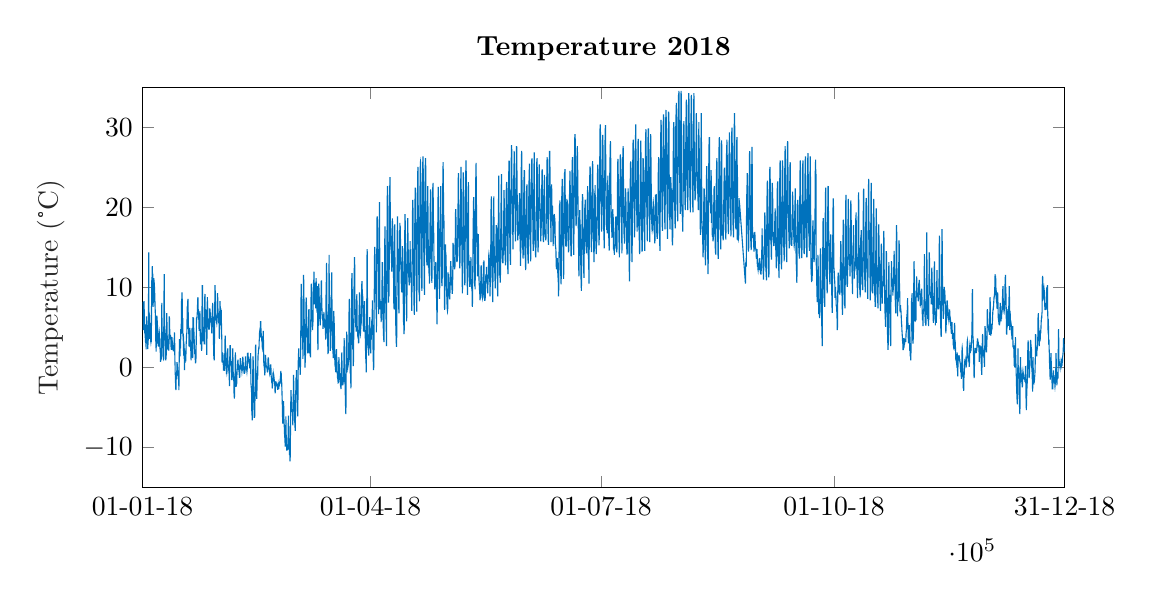
\begin{tikzpicture}

\begin{axis}[%
width=4.61in,
height=2in,
at={(0.758in,0.481in)},
scale only axis,
xmin=737061,
xmax=737425,
xtick={736969,737061,737151,737242,737334,737425},
xticklabels={{01-10-17},{01-01-18},{01-04-18},{01-07-18},{01-10-18},{31-12-18}},
ymin=-15,
ymax=35,
ylabel style={font=\color{white!15!black}},
ylabel={Temperature (°C)},
axis background/.style={fill=white},
title style={font=\bfseries},
title={Temperature 2018},
legend style={legend cell align=left, align=left, draw=white!15!black}
]
\addplot [color=mycolor1, forget plot]
  table[row sep=crcr]{%
737061	6.1\\
737061.034722222	5.1\\
737061.069444444	6.2\\
737061.104166667	8.2\\
737061.138888889	6.9\\
737061.173611111	5.2\\
737061.208333333	4.7\\
737061.243055556	5.4\\
737061.277777778	5.4\\
737061.3125	5.3\\
737061.347222222	5.7\\
737061.381944444	5.5\\
737061.416666667	4.7\\
737061.451388889	6\\
737061.486111111	6.5\\
737061.520833333	7.2\\
737061.555555556	7.9\\
737061.590277778	8.3\\
737061.625	7.8\\
737061.659722222	7.1\\
737061.694444444	6.4\\
737061.729166667	5.2\\
737061.763888889	5.4\\
737061.798611111	5\\
737061.833333333	4.8\\
737061.868055556	4.6\\
737061.902777778	4.2\\
737061.9375	5.2\\
737061.972222222	5.2\\
737062.006944444	5.4\\
737062.041666667	4.7\\
737062.076388889	4\\
737062.111111111	3.2\\
737062.145833333	3.4\\
737062.184027778	3.4\\
737062.21875	3.2\\
737062.253472222	3.1\\
737062.288194444	3.4\\
737062.322916667	3.4\\
737062.357638889	3.6\\
737062.392361111	2.3\\
737062.427083333	2.6\\
737062.461805556	3.7\\
737062.496527778	4.8\\
737062.53125	5.5\\
737062.565972222	6.4\\
737062.600694444	5.6\\
737062.635416667	5.9\\
737062.670138889	5.6\\
737062.704861111	5.4\\
737062.739583333	5.3\\
737062.774305556	4.7\\
737062.809027778	4.6\\
737062.84375	4.4\\
737062.878472222	4.2\\
737062.913194444	3.9\\
737062.947916667	4.1\\
737062.982638889	2.9\\
737063.017361111	2.4\\
737063.052083333	2.4\\
737063.086805556	2.7\\
737063.121527778	2.8\\
737063.15625	3\\
737063.190972222	3.6\\
737063.225694444	3.3\\
737063.260416667	4.4\\
737063.295138889	5.4\\
737063.329861111	6.1\\
737063.364583333	8.8\\
737063.399305556	11.6\\
737063.434027778	14.4\\
737063.46875	11.7\\
737063.503472222	10.9\\
737063.538194444	4.8\\
737063.572916667	5.2\\
737063.607638889	5.9\\
737063.642361111	4.3\\
737063.677083333	6.7\\
737063.711805556	6.7\\
737063.746527778	6.3\\
737063.78125	6.3\\
737063.815972222	3.6\\
737063.850694444	3.7\\
737063.885416667	5.2\\
737063.920138889	5.6\\
737063.954861111	4.5\\
737063.989583333	4.1\\
737064.027777778	4.6\\
737064.0625	5.1\\
737064.097222222	4.9\\
737064.131944444	4.2\\
737064.166666667	3.7\\
737064.201388889	3.4\\
737064.236111111	3.3\\
737064.270833333	3.3\\
737064.305555556	3.2\\
737064.34375	3.3\\
737064.378472222	3.3\\
737064.413194444	3.2\\
737064.447916667	3.6\\
737064.482638889	4.2\\
737064.517361111	5.4\\
737064.552083333	7.5\\
737064.586805556	10\\
737064.621527778	10.8\\
737064.65625	10.9\\
737064.690972222	11.3\\
737064.725694444	11.2\\
737064.760416667	11.2\\
737064.795138889	11.8\\
737064.829861111	12.5\\
737064.864583333	12.7\\
737064.899305556	11.9\\
737064.934027778	11.8\\
737064.96875	11.5\\
737065.003472222	11.7\\
737065.038194444	11.3\\
737065.072916667	10.4\\
737065.107638889	8.4\\
737065.142361111	7.8\\
737065.177083333	7.6\\
737065.211805556	8.2\\
737065.246527778	9.8\\
737065.28125	10.2\\
737065.315972222	9.7\\
737065.350694444	8.5\\
737065.385416667	8.2\\
737065.420138889	9.3\\
737065.454861111	10.7\\
737065.489583333	11.2\\
737065.524305556	10.4\\
737065.559027778	10.7\\
737065.59375	10.7\\
737065.628472222	10.1\\
737065.663194444	10.1\\
737065.697916667	10.1\\
737065.732638889	9.6\\
737065.767361111	8.9\\
737065.802083333	8.8\\
737065.836805556	9.3\\
737065.871527778	8.8\\
737065.90625	8\\
737065.940972222	7.6\\
737065.975694444	7.4\\
737066.013888889	7.1\\
737066.048611111	6.7\\
737066.083333333	6.4\\
737066.118055556	5.6\\
737066.152777778	5.1\\
737066.1875	3.9\\
737066.222222222	3.4\\
737066.256944444	3\\
737066.291666667	2.8\\
737066.326388889	2.5\\
737066.361111111	2\\
737066.395833333	2.7\\
737066.430555556	4.4\\
737066.465277778	5.3\\
737066.5	5.8\\
737066.534722222	6\\
737066.569444444	6.3\\
737066.604166667	6.5\\
737066.638888889	6.4\\
737066.673611111	6.3\\
737066.708333333	6.3\\
737066.743055556	6.2\\
737066.777777778	5.9\\
737066.8125	5.8\\
737066.847222222	5.4\\
737066.881944444	5.3\\
737066.916666667	5.2\\
737066.951388889	4\\
737066.986111111	3\\
737067.024305556	3.4\\
737067.059027778	3.4\\
737067.09375	3.4\\
737067.128472222	3.4\\
737067.163194444	3.3\\
737067.201388889	2.8\\
737067.236111111	2.8\\
737067.270833333	2.7\\
737067.305555556	2.7\\
737067.340277778	2.8\\
737067.375	2.7\\
737067.409722222	2.7\\
737067.444444444	3.5\\
737067.479166667	4.2\\
737067.513888889	4.3\\
737067.548611111	4.4\\
737067.583333333	4.5\\
737067.618055556	4.4\\
737067.652777778	4.5\\
737067.6875	4.2\\
737067.722222222	3.9\\
737067.756944444	3.7\\
737067.791666667	3.4\\
737067.826388889	3.2\\
737067.861111111	2.4\\
737067.895833333	2.4\\
737067.930555556	2.3\\
737067.965277778	2.2\\
737068	2\\
737068.034722222	1.6\\
737068.069444444	1.6\\
737068.104166667	0.8\\
737068.138888889	0.8\\
737068.173611111	1.3\\
737068.208333333	1.3\\
737068.243055556	1.5\\
737068.277777778	1.5\\
737068.3125	1.2\\
737068.347222222	0.9\\
737068.381944444	1.3\\
737068.416666667	1.7\\
737068.451388889	2.2\\
737068.486111111	3.1\\
737068.520833333	4.4\\
737068.555555556	5.2\\
737068.590277778	7.7\\
737068.625	8.1\\
737068.659722222	6.1\\
737068.694444444	5.2\\
737068.729166667	4.7\\
737068.763888889	4.4\\
737068.798611111	3.8\\
737068.833333333	3.5\\
737068.868055556	3.2\\
737068.902777778	3.1\\
737068.9375	3.7\\
737068.972222222	3\\
737069.010416667	2.6\\
737069.045138889	2.2\\
737069.079861111	1.4\\
737069.114583333	1.5\\
737069.149305556	1.4\\
737069.1875	1.5\\
737069.222222222	2.4\\
737069.256944444	2.4\\
737069.291666667	2.1\\
737069.326388889	0.9\\
737069.361111111	1.2\\
737069.395833333	5.7\\
737069.430555556	9.6\\
737069.465277778	7.2\\
737069.5	8.2\\
737069.534722222	10.3\\
737069.569444444	11.7\\
737069.604166667	8\\
737069.638888889	7.1\\
737069.673611111	6.6\\
737069.708333333	5.4\\
737069.743055556	4.8\\
737069.777777778	4.5\\
737069.8125	4.5\\
737069.847222222	3.6\\
737069.881944444	3.6\\
737069.916666667	3.4\\
737069.951388889	4.1\\
737069.986111111	4.3\\
737070.020833333	4.2\\
737070.055555556	3.3\\
737070.090277778	2.5\\
737070.125	1.9\\
737070.159722222	0.9\\
737070.197916667	1.1\\
737070.232638889	1\\
737070.267361111	1.7\\
737070.302083333	1.8\\
737070.336805556	1.6\\
737070.371527778	1.6\\
737070.40625	2.2\\
737070.440972222	3.8\\
737070.475694444	5.2\\
737070.510416667	6.1\\
737070.545138889	6.8\\
737070.579861111	6.5\\
737070.614583333	5.9\\
737070.649305556	5.5\\
737070.684027778	4.6\\
737070.71875	3.9\\
737070.753472222	4\\
737070.788194444	3.8\\
737070.822916667	3.6\\
737070.857638889	3.4\\
737070.892361111	3.3\\
737070.927083333	2.7\\
737070.961805556	2.4\\
737070.996527778	2.2\\
737071.03125	2.3\\
737071.065972222	3.2\\
737071.100694444	3.4\\
737071.135416667	2.9\\
737071.173611111	2.4\\
737071.208333333	2.3\\
737071.243055556	2.6\\
737071.277777778	2.7\\
737071.3125	2.4\\
737071.347222222	2.2\\
737071.381944444	2.2\\
737071.416666667	2.8\\
737071.451388889	3.9\\
737071.486111111	4.6\\
737071.520833333	5.7\\
737071.555555556	6.4\\
737071.590277778	6.3\\
737071.625	6.2\\
737071.659722222	6.1\\
737071.694444444	5.5\\
737071.729166667	4.5\\
737071.763888889	4\\
737071.798611111	3.7\\
737071.833333333	3.6\\
737071.868055556	3.6\\
737071.902777778	3.7\\
737071.9375	3.8\\
737071.972222222	3.9\\
737072.006944444	4.1\\
737072.041666667	3.8\\
737072.076388889	3.9\\
737072.111111111	3.9\\
737072.145833333	3.6\\
737072.184027778	3.3\\
737072.21875	3.1\\
737072.253472222	2.6\\
737072.288194444	2.3\\
737072.322916667	2.5\\
737072.357638889	2.6\\
737072.392361111	2.3\\
737072.427083333	2.3\\
737072.461805556	2.7\\
737072.496527778	3.2\\
737072.53125	3.6\\
737072.565972222	3.8\\
737072.600694444	3.7\\
737072.635416667	3.7\\
737072.670138889	3.5\\
737072.704861111	3.3\\
737072.739583333	3.3\\
737072.774305556	3.2\\
737072.809027778	3.1\\
737072.84375	2.9\\
737072.878472222	2.7\\
737072.913194444	2.5\\
737072.947916667	2.4\\
737072.982638889	2.4\\
737073.017361111	2.4\\
737073.052083333	2.2\\
737073.086805556	2.3\\
737073.121527778	2.2\\
737073.15625	2.2\\
737073.194444444	2.1\\
737073.229166667	2.1\\
737073.263888889	2.1\\
737073.298611111	2.1\\
737073.333333333	2.1\\
737073.368055556	2.1\\
737073.402777778	2.3\\
737073.4375	2.8\\
737073.472222222	3.1\\
737073.506944444	3.3\\
737073.541666667	3.8\\
737073.576388889	4.4\\
737073.611111111	4.3\\
737073.645833333	3.8\\
737073.680555556	3.6\\
737073.715277778	2\\
737073.75	1.2\\
737073.784722222	0.8\\
737073.819444444	0.4\\
737073.854166667	0.1\\
737073.888888889	-0.9\\
737073.923611111	-0.7\\
737073.958333333	-0.6\\
737073.993055556	-1.3\\
737074.027777778	-1.9\\
737074.0625	-2.3\\
737074.097222222	-2.6\\
737074.131944444	-2.6\\
737074.166666667	-2.8\\
737074.204861111	-2.7\\
737074.239583333	-1.7\\
737074.274305556	-1.3\\
737074.309027778	-1.4\\
737074.34375	-1.4\\
737074.378472222	-1.3\\
737074.413194444	-1.4\\
737074.447916667	-1.2\\
737074.482638889	-1\\
737074.517361111	-0.4\\
737074.552083333	-0.3\\
737074.586805556	0\\
737074.621527778	0.7\\
737074.65625	0.5\\
737074.690972222	0.4\\
737074.725694444	0.4\\
737074.760416667	0.2\\
737074.795138889	0\\
737074.829861111	-0.2\\
737074.864583333	-0.3\\
737074.899305556	-0.4\\
737074.934027778	-0.4\\
737074.96875	-0.4\\
737075.003472222	-0.5\\
737075.038194444	-0.6\\
737075.072916667	-0.8\\
737075.107638889	-1\\
737075.142361111	-1.2\\
737075.177083333	-1.3\\
737075.211805556	-1.5\\
737075.246527778	-1.6\\
737075.28125	-1.7\\
737075.315972222	-2.3\\
737075.350694444	-2.8\\
737075.385416667	-1.9\\
737075.420138889	-0.9\\
737075.454861111	0.1\\
737075.489583333	1.6\\
737075.524305556	2.3\\
737075.559027778	3.3\\
737075.59375	3.5\\
737075.628472222	3.5\\
737075.663194444	3.4\\
737075.697916667	2.8\\
737075.732638889	2.1\\
737075.767361111	1.4\\
737075.802083333	1.7\\
737075.836805556	2.7\\
737075.871527778	2.8\\
737075.90625	3.3\\
737075.940972222	3.1\\
737075.975694444	2.6\\
737076.013888889	2.4\\
737076.048611111	2.9\\
737076.083333333	4.8\\
737076.118055556	4.3\\
737076.152777778	4.6\\
737076.190972222	4.7\\
737076.225694444	4.3\\
737076.260416667	4.3\\
737076.295138889	5.1\\
737076.329861111	8.1\\
737076.364583333	8.2\\
737076.399305556	8.1\\
737076.434027778	7.4\\
737076.46875	7.3\\
737076.503472222	7.7\\
737076.538194444	8.8\\
737076.572916667	9.4\\
737076.607638889	9.2\\
737076.642361111	9.1\\
737076.677083333	7.4\\
737076.711805556	5.8\\
737076.746527778	4.9\\
737076.78125	4.5\\
737076.815972222	4.3\\
737076.850694444	6.2\\
737076.885416667	4.5\\
737076.920138889	5.1\\
737076.954861111	3.9\\
737076.989583333	4.2\\
737077.024305556	4.3\\
737077.059027778	3.9\\
737077.09375	3.3\\
737077.128472222	4.2\\
737077.163194444	3.6\\
737077.197916667	1.5\\
737077.232638889	2.4\\
737077.267361111	2.4\\
737077.302083333	2.8\\
737077.336805556	2.8\\
737077.371527778	2.9\\
737077.40625	2.8\\
737077.440972222	1.1\\
737077.475694444	1.4\\
737077.510416667	1.6\\
737077.545138889	-0.3\\
737077.579861111	0.5\\
737077.614583333	2.4\\
737077.649305556	2\\
737077.684027778	1.2\\
737077.71875	1.2\\
737077.753472222	1.6\\
737077.788194444	0.6\\
737077.822916667	0.9\\
737077.857638889	1.9\\
737077.892361111	1.9\\
737077.927083333	1.6\\
737077.961805556	1.6\\
737078	1.7\\
737078.034722222	1.1\\
737078.069444444	0.8\\
737078.104166667	1.6\\
737078.138888889	1.7\\
737078.173611111	2.1\\
737078.208333333	2.9\\
737078.243055556	3\\
737078.277777778	3.3\\
737078.3125	3.4\\
737078.347222222	3.9\\
737078.381944444	4.2\\
737078.416666667	4.2\\
737078.451388889	4.3\\
737078.486111111	4.3\\
737078.520833333	4.7\\
737078.555555556	5.4\\
737078.590277778	6.9\\
737078.625	7.3\\
737078.659722222	7.6\\
737078.694444444	7.7\\
737078.729166667	7\\
737078.763888889	7\\
737078.798611111	7.5\\
737078.833333333	7.8\\
737078.868055556	8.4\\
737078.902777778	7.9\\
737078.9375	8.6\\
737078.972222222	8.2\\
737079.010416667	6\\
737079.045138889	6.2\\
737079.079861111	6.9\\
737079.114583333	5.3\\
737079.149305556	4.9\\
737079.1875	4.6\\
737079.222222222	4.2\\
737079.256944444	4.3\\
737079.291666667	3.4\\
737079.326388889	3.2\\
737079.361111111	2.7\\
737079.395833333	2.7\\
737079.430555556	3.6\\
737079.465277778	3.9\\
737079.5	4.2\\
737079.534722222	4.5\\
737079.569444444	4.6\\
737079.604166667	4.9\\
737079.638888889	4.9\\
737079.673611111	4.9\\
737079.708333333	4.7\\
737079.743055556	4.4\\
737079.777777778	2.6\\
737079.8125	2.6\\
737079.847222222	3.4\\
737079.881944444	3.4\\
737079.916666667	3.1\\
737079.951388889	2.9\\
737079.986111111	2.8\\
737080.020833333	2.1\\
737080.055555556	2.4\\
737080.090277778	2.2\\
737080.125	1.5\\
737080.159722222	0.9\\
737080.197916667	1.2\\
737080.232638889	1.4\\
737080.267361111	2.2\\
737080.302083333	2.3\\
737080.336805556	2.7\\
737080.371527778	2.8\\
737080.40625	2.9\\
737080.440972222	3.2\\
737080.475694444	3.7\\
737080.510416667	4.4\\
737080.545138889	4.9\\
737080.579861111	4.9\\
737080.614583333	4.6\\
737080.649305556	4.3\\
737080.684027778	4.1\\
737080.71875	2.7\\
737080.753472222	1.7\\
737080.788194444	1.2\\
737080.822916667	1.5\\
737080.857638889	4.8\\
737080.892361111	5.8\\
737080.927083333	6.3\\
737080.961805556	5.8\\
737080.996527778	5.8\\
737081.03125	6.2\\
737081.065972222	6\\
737081.100694444	6.2\\
737081.135416667	6.1\\
737081.170138889	5.5\\
737081.204861111	4.7\\
737081.239583333	4.4\\
737081.274305556	4.6\\
737081.309027778	4.3\\
737081.34375	4.2\\
737081.378472222	3.6\\
737081.413194444	3.4\\
737081.447916667	2.7\\
737081.482638889	2.7\\
737081.517361111	2.7\\
737081.552083333	1.7\\
737081.586805556	2.1\\
737081.621527778	2.2\\
737081.65625	2.1\\
737081.690972222	1.9\\
737081.725694444	1.7\\
737081.760416667	1.7\\
737081.795138889	1.6\\
737081.829861111	0.9\\
737081.864583333	0.6\\
737081.899305556	0.6\\
737081.934027778	0.6\\
737081.96875	0.6\\
737082.006944444	0.8\\
737082.041666667	1.1\\
737082.076388889	1.1\\
737082.111111111	1.3\\
737082.145833333	1.8\\
737082.180555556	2.9\\
737082.215277778	3.8\\
737082.25	4.7\\
737082.284722222	5.7\\
737082.319444444	6.2\\
737082.354166667	6.2\\
737082.388888889	6\\
737082.423611111	6.2\\
737082.458333333	6.2\\
737082.493055556	6.3\\
737082.527777778	6.3\\
737082.5625	6.8\\
737082.597222222	6.9\\
737082.631944444	6.7\\
737082.666666667	6.9\\
737082.701388889	7.7\\
737082.736111111	8.1\\
737082.770833333	8.6\\
737082.805555556	8.6\\
737082.840277778	8.8\\
737082.875	8.7\\
737082.909722222	8\\
737082.944444444	7.6\\
737082.979166667	7.2\\
737083.017361111	7.1\\
737083.052083333	7\\
737083.086805556	6.7\\
737083.121527778	6.6\\
737083.15625	6.7\\
737083.190972222	6.4\\
737083.225694444	5.6\\
737083.260416667	5.3\\
737083.295138889	5\\
737083.329861111	4.6\\
737083.364583333	4.8\\
737083.399305556	5.2\\
737083.434027778	5.4\\
737083.46875	5.7\\
737083.503472222	6.1\\
737083.538194444	6.3\\
737083.572916667	6.4\\
737083.607638889	6.7\\
737083.642361111	7.1\\
737083.677083333	6.4\\
737083.711805556	5.8\\
737083.746527778	5.1\\
737083.78125	4.3\\
737083.815972222	3.6\\
737083.850694444	3.1\\
737083.885416667	2.9\\
737083.920138889	3\\
737083.954861111	3.3\\
737083.989583333	3.1\\
737084.027777778	3.3\\
737084.0625	3.4\\
737084.097222222	4.3\\
737084.131944444	4.3\\
737084.166666667	4.2\\
737084.204861111	3.6\\
737084.239583333	2.8\\
737084.274305556	2.3\\
737084.309027778	2.2\\
737084.34375	2.1\\
737084.378472222	3.1\\
737084.413194444	4.7\\
737084.447916667	6.1\\
737084.482638889	7.3\\
737084.517361111	8.8\\
737084.552083333	10\\
737084.586805556	10.3\\
737084.621527778	10.2\\
737084.65625	10.3\\
737084.690972222	9.9\\
737084.725694444	7.8\\
737084.760416667	7.3\\
737084.795138889	4.5\\
737084.829861111	4.5\\
737084.864583333	3.9\\
737084.899305556	4.8\\
737084.934027778	3.3\\
737084.96875	3.8\\
737085.003472222	4.9\\
737085.038194444	4.6\\
737085.072916667	4.3\\
737085.107638889	3.7\\
737085.142361111	3.5\\
737085.180555556	3.4\\
737085.215277778	4.7\\
737085.25	5.1\\
737085.284722222	4.3\\
737085.319444444	3.9\\
737085.354166667	2.9\\
737085.388888889	4\\
737085.423611111	4\\
737085.458333333	5.2\\
737085.493055556	7.1\\
737085.527777778	8.3\\
737085.5625	8.8\\
737085.597222222	9\\
737085.631944444	9.1\\
737085.666666667	9.2\\
737085.701388889	8.2\\
737085.736111111	6.9\\
737085.770833333	6.2\\
737085.805555556	5.9\\
737085.840277778	5.7\\
737085.875	7.1\\
737085.909722222	7.3\\
737085.944444444	7.1\\
737085.979166667	6.4\\
737086.013888889	5.7\\
737086.048611111	5.2\\
737086.083333333	4.7\\
737086.118055556	3.2\\
737086.152777778	2.9\\
737086.190972222	3.4\\
737086.225694444	3.2\\
737086.260416667	2.9\\
737086.295138889	2.9\\
737086.329861111	1.9\\
737086.364583333	1.6\\
737086.399305556	2.3\\
737086.434027778	4.2\\
737086.46875	5.8\\
737086.506944444	6.7\\
737086.541666667	7.2\\
737086.576388889	8.8\\
737086.611111111	8.1\\
737086.645833333	8.4\\
737086.680555556	8.3\\
737086.715277778	7.5\\
737086.75	7.4\\
737086.784722222	6.6\\
737086.819444444	6.1\\
737086.854166667	5.8\\
737086.888888889	5.6\\
737086.923611111	5.4\\
737086.958333333	5.3\\
737086.993055556	5.3\\
737087.027777778	5.1\\
737087.0625	5.1\\
737087.097222222	5\\
737087.131944444	4.9\\
737087.166666667	4.9\\
737087.204861111	4.8\\
737087.239583333	4.8\\
737087.274305556	4.9\\
737087.309027778	4.9\\
737087.34375	4.9\\
737087.378472222	5.3\\
737087.413194444	5.7\\
737087.447916667	6.1\\
737087.482638889	6.6\\
737087.517361111	7.1\\
737087.552083333	7.4\\
737087.586805556	7.3\\
737087.621527778	7.2\\
737087.65625	7.2\\
737087.690972222	7.1\\
737087.725694444	6.7\\
737087.760416667	6.5\\
737087.795138889	6.3\\
737087.829861111	5.9\\
737087.864583333	5.8\\
737087.899305556	5.8\\
737087.934027778	5.8\\
737087.96875	5.8\\
737088.003472222	5.7\\
737088.038194444	5.8\\
737088.072916667	5.7\\
737088.107638889	5.6\\
737088.142361111	5.3\\
737088.180555556	5.3\\
737088.215277778	5.2\\
737088.25	5.1\\
737088.284722222	4.8\\
737088.319444444	4.3\\
737088.354166667	4.4\\
737088.388888889	5\\
737088.423611111	5.3\\
737088.458333333	5.8\\
737088.493055556	6.7\\
737088.527777778	6.8\\
737088.5625	7.1\\
737088.597222222	7.4\\
737088.631944444	7.7\\
737088.666666667	8.1\\
737088.701388889	7.9\\
737088.736111111	6.7\\
737088.770833333	5.8\\
737088.805555556	5.7\\
737088.840277778	6.2\\
737088.875	6.4\\
737088.909722222	6.3\\
737088.944444444	5.1\\
737088.979166667	4.8\\
737089.013888889	3.9\\
737089.048611111	1.8\\
737089.083333333	1.7\\
737089.118055556	1.7\\
737089.152777778	1.1\\
737089.190972222	1.6\\
737089.225694444	1.1\\
737089.260416667	1.3\\
737089.295138889	0.9\\
737089.329861111	1.5\\
737089.364583333	1.8\\
737089.399305556	3.9\\
737089.434027778	5.8\\
737089.46875	6.7\\
737089.503472222	7.4\\
737089.538194444	8.7\\
737089.572916667	9.3\\
737089.607638889	10.3\\
737089.642361111	10.1\\
737089.677083333	9.8\\
737089.711805556	7.9\\
737089.746527778	6.4\\
737089.78125	6.1\\
737089.815972222	6.6\\
737089.850694444	6.3\\
737089.885416667	6.2\\
737089.920138889	5.9\\
737089.954861111	6\\
737089.989583333	6\\
737090.024305556	6.1\\
737090.059027778	6\\
737090.09375	6\\
737090.128472222	5.8\\
737090.163194444	5.9\\
737090.197916667	5.7\\
737090.232638889	5.5\\
737090.267361111	5.6\\
737090.302083333	5.7\\
737090.336805556	5.6\\
737090.371527778	5.7\\
737090.40625	6.1\\
737090.440972222	7.3\\
737090.475694444	8.2\\
737090.510416667	8.2\\
737090.545138889	8.4\\
737090.579861111	9.1\\
737090.614583333	9.3\\
737090.649305556	9.1\\
737090.684027778	8.5\\
737090.71875	7.9\\
737090.753472222	7.3\\
737090.788194444	7.3\\
737090.822916667	7\\
737090.857638889	6.9\\
737090.892361111	6.6\\
737090.927083333	6.2\\
737090.961805556	6.3\\
737091	6.2\\
737091.034722222	6.1\\
737091.069444444	5.9\\
737091.104166667	5.6\\
737091.138888889	5.7\\
737091.173611111	5.6\\
737091.208333333	5.7\\
737091.243055556	5.2\\
737091.277777778	3.8\\
737091.3125	3.7\\
737091.347222222	3.6\\
737091.381944444	4.3\\
737091.416666667	5.5\\
737091.451388889	6.4\\
737091.486111111	6.8\\
737091.520833333	7.5\\
737091.555555556	8.2\\
737091.590277778	8.3\\
737091.625	7.9\\
737091.659722222	7.6\\
737091.694444444	7.3\\
737091.729166667	7.2\\
737091.763888889	6.7\\
737091.798611111	5.9\\
737091.833333333	5.3\\
737091.868055556	6.3\\
737091.902777778	7.4\\
737091.9375	6.5\\
737091.972222222	6.2\\
737092.010416667	6.2\\
737092.045138889	7.1\\
737092.079861111	7.2\\
737092.114583333	6.4\\
737092.149305556	5.5\\
737092.184027778	4.9\\
737092.21875	4.3\\
737092.253472222	4.1\\
737092.288194444	3.6\\
737092.322916667	0.9\\
737092.357638889	1\\
737092.392361111	0.7\\
737092.427083333	0.7\\
737092.461805556	0.8\\
737092.496527778	1.3\\
737092.53125	1.9\\
737092.565972222	1.7\\
737092.600694444	1.8\\
737092.635416667	1.4\\
737092.670138889	1.6\\
737092.704861111	1.8\\
737092.739583333	1.6\\
737092.774305556	1.4\\
737092.809027778	1.3\\
737092.84375	0.8\\
737092.878472222	0.4\\
737092.913194444	-0.2\\
737092.947916667	-0.3\\
737092.982638889	-0.3\\
737093.020833333	-0.1\\
737093.055555556	0.3\\
737093.090277778	0.3\\
737093.125	0.4\\
737093.159722222	0.4\\
737093.197916667	0.3\\
737093.232638889	0.2\\
737093.267361111	0.2\\
737093.302083333	0\\
737093.336805556	-0.4\\
737093.371527778	-0.3\\
737093.40625	0.2\\
737093.440972222	1.3\\
737093.475694444	1.8\\
737093.510416667	3.2\\
737093.545138889	2.9\\
737093.579861111	3.8\\
737093.614583333	3.8\\
737093.649305556	4\\
737093.684027778	3.2\\
737093.71875	2.9\\
737093.753472222	2.4\\
737093.788194444	2.1\\
737093.822916667	1.9\\
737093.857638889	1.6\\
737093.892361111	1.5\\
737093.927083333	1.2\\
737093.961805556	0.3\\
737093.996527778	0.3\\
737094.03125	0.5\\
737094.065972222	-0.2\\
737094.100694444	-0.8\\
737094.135416667	-0.4\\
737094.173611111	-0.6\\
737094.208333333	-0.5\\
737094.243055556	-0.5\\
737094.277777778	-0.6\\
737094.3125	-0.5\\
737094.347222222	-0.5\\
737094.381944444	-0.1\\
737094.416666667	0.6\\
737094.451388889	0.9\\
737094.486111111	1.5\\
737094.520833333	1.8\\
737094.555555556	2.1\\
737094.590277778	2.1\\
737094.625	2.4\\
737094.659722222	2.3\\
737094.694444444	1.2\\
737094.729166667	0.6\\
737094.763888889	0.5\\
737094.798611111	0.4\\
737094.833333333	0.3\\
737094.868055556	0.1\\
737094.902777778	0.1\\
737094.9375	0.2\\
737094.972222222	-0.2\\
737095.006944444	-0.3\\
737095.041666667	-0.3\\
737095.076388889	-0.5\\
737095.111111111	-0.6\\
737095.145833333	-0.7\\
737095.184027778	-0.8\\
737095.21875	-1.2\\
737095.253472222	-1.6\\
737095.288194444	-1.9\\
737095.322916667	-2.3\\
737095.357638889	-1.7\\
737095.392361111	-0.3\\
737095.427083333	0.9\\
737095.461805556	1.7\\
737095.496527778	2.2\\
737095.53125	2.7\\
737095.565972222	2.7\\
737095.600694444	2.6\\
737095.635416667	2.8\\
737095.670138889	2.7\\
737095.704861111	2.4\\
737095.739583333	1.3\\
737095.774305556	0.4\\
737095.809027778	0.3\\
737095.84375	0.5\\
737095.878472222	0.7\\
737095.913194444	0.8\\
737095.947916667	0.6\\
737095.982638889	0.3\\
737096.017361111	0.4\\
737096.052083333	0.3\\
737096.086805556	0.1\\
737096.121527778	-0.3\\
737096.15625	-0.9\\
737096.190972222	-1.5\\
737096.225694444	-1.5\\
737096.260416667	-1.5\\
737096.295138889	-1.5\\
737096.329861111	-1.3\\
737096.364583333	-1.4\\
737096.399305556	-0.8\\
737096.434027778	-0.6\\
737096.46875	0\\
737096.503472222	0.8\\
737096.538194444	0.6\\
737096.572916667	1.3\\
737096.607638889	2.4\\
737096.642361111	2.1\\
737096.677083333	1.6\\
737096.711805556	0.6\\
737096.746527778	-0.2\\
737096.78125	-0.5\\
737096.815972222	-0.8\\
737096.850694444	-0.8\\
737096.885416667	-1.1\\
737096.920138889	-1.2\\
737096.954861111	-1.3\\
737096.989583333	-1.4\\
737097.027777778	-1.7\\
737097.0625	-2.2\\
737097.097222222	-2.9\\
737097.131944444	-3.3\\
737097.166666667	-2.9\\
737097.204861111	-3.6\\
737097.239583333	-3.8\\
737097.274305556	-3.8\\
737097.309027778	-2.9\\
737097.34375	-2.6\\
737097.378472222	-2.2\\
737097.413194444	-1.6\\
737097.447916667	-1.6\\
737097.482638889	-1.2\\
737097.517361111	-0.8\\
737097.552083333	-0.1\\
737097.586805556	1.6\\
737097.621527778	1.3\\
737097.65625	1.9\\
737097.690972222	1.3\\
737097.725694444	0.4\\
737097.760416667	-0.8\\
737097.795138889	-1.4\\
737097.829861111	-1.8\\
737097.864583333	-2\\
737097.899305556	-2.4\\
737097.934027778	-2.3\\
737097.96875	-2.2\\
737098.003472222	-2.3\\
737098.038194444	-2.1\\
737098.072916667	-2.1\\
737098.107638889	-2\\
737098.142361111	-1.9\\
737098.180555556	-2\\
737098.215277778	-1.4\\
737098.25	-1.1\\
737098.284722222	-0.7\\
737098.319444444	-0.4\\
737098.354166667	-0.3\\
737098.388888889	-0.2\\
737098.423611111	-0.1\\
737098.458333333	0.1\\
737098.493055556	0.3\\
737098.527777778	0.6\\
737098.5625	0.6\\
737098.597222222	0.8\\
737098.631944444	0.8\\
737098.666666667	1\\
737098.701388889	0.8\\
737098.736111111	0.6\\
737098.770833333	0.4\\
737098.805555556	0.4\\
737098.840277778	0.2\\
737098.875	0.2\\
737098.909722222	0.1\\
737098.944444444	-0.1\\
737098.979166667	-0.2\\
737099.013888889	-0.3\\
737099.048611111	-0.3\\
737099.083333333	-0.4\\
737099.118055556	-0.7\\
737099.152777778	-0.7\\
737099.190972222	-0.9\\
737099.225694444	-1.1\\
737099.260416667	-1.2\\
737099.295138889	-1.2\\
737099.329861111	-1.1\\
737099.364583333	-1.1\\
737099.399305556	-0.8\\
737099.434027778	-0.2\\
737099.46875	0.2\\
737099.503472222	0.4\\
737099.538194444	0.6\\
737099.572916667	1.1\\
737099.607638889	1.1\\
737099.642361111	1.2\\
737099.677083333	0.8\\
737099.711805556	0.7\\
737099.746527778	0.5\\
737099.78125	0.3\\
737099.815972222	0.3\\
737099.850694444	0.3\\
737099.885416667	0.2\\
737099.920138889	0.1\\
737099.954861111	-0.1\\
737099.989583333	-0.1\\
737100.024305556	-0.2\\
737100.059027778	-0.2\\
737100.09375	-0.2\\
737100.128472222	-0.3\\
737100.163194444	-0.3\\
737100.197916667	-0.4\\
737100.232638889	-0.5\\
737100.267361111	-0.4\\
737100.302083333	-0.4\\
737100.336805556	-0.4\\
737100.371527778	-0.2\\
737100.40625	0\\
737100.440972222	0.4\\
737100.475694444	0.8\\
737100.510416667	1\\
737100.545138889	1.2\\
737100.579861111	1.3\\
737100.614583333	1.3\\
737100.649305556	1.1\\
737100.684027778	1.1\\
737100.71875	0.8\\
737100.753472222	0.5\\
737100.788194444	0.1\\
737100.822916667	-0.2\\
737100.857638889	-0.3\\
737100.892361111	-0.1\\
737100.927083333	0.1\\
737100.961805556	0.1\\
737101	-0.1\\
737101.034722222	-0.4\\
737101.069444444	-0.6\\
737101.104166667	-0.7\\
737101.138888889	-0.7\\
737101.177083333	-0.3\\
737101.211805556	-0.4\\
737101.246527778	-0.4\\
737101.28125	-0.4\\
737101.315972222	-0.6\\
737101.350694444	-0.6\\
737101.385416667	-0.5\\
737101.420138889	-0.4\\
737101.454861111	-0.4\\
737101.489583333	0.2\\
737101.524305556	0.4\\
737101.559027778	0.6\\
737101.59375	0.9\\
737101.628472222	1.4\\
737101.663194444	1.1\\
737101.697916667	0.9\\
737101.732638889	0.8\\
737101.767361111	0.4\\
737101.802083333	0.2\\
737101.836805556	-0.2\\
737101.871527778	0\\
737101.90625	0.1\\
737101.940972222	0.1\\
737101.975694444	-0.1\\
737102.010416667	-0.1\\
737102.045138889	-0.2\\
737102.079861111	-0.3\\
737102.114583333	-0.3\\
737102.149305556	-0.3\\
737102.184027778	-0.4\\
737102.21875	-0.5\\
737102.253472222	-0.4\\
737102.288194444	-0.3\\
737102.322916667	-0.2\\
737102.357638889	0.2\\
737102.392361111	1.1\\
737102.427083333	1.8\\
737102.461805556	1.1\\
737102.496527778	1.4\\
737102.53125	0.7\\
737102.565972222	1.1\\
737102.600694444	1.8\\
737102.635416667	1.8\\
737102.670138889	1.3\\
737102.704861111	1.1\\
737102.739583333	0.8\\
737102.774305556	0.9\\
737102.809027778	0.8\\
737102.84375	0.8\\
737102.878472222	0.8\\
737102.913194444	1.3\\
737102.947916667	1.3\\
737102.982638889	1.2\\
737103.020833333	0.5\\
737103.055555556	0.6\\
737103.090277778	0.7\\
737103.125	0.8\\
737103.159722222	0.5\\
737103.197916667	0.3\\
737103.232638889	0.3\\
737103.267361111	0.3\\
737103.302083333	0.1\\
737103.336805556	-0.1\\
737103.371527778	0.1\\
737103.40625	0.1\\
737103.440972222	0.1\\
737103.475694444	0.9\\
737103.510416667	1.1\\
737103.545138889	0\\
737103.579861111	0.6\\
737103.614583333	0.4\\
737103.649305556	0.2\\
737103.684027778	1.8\\
737103.71875	-0.1\\
737103.753472222	-1.3\\
737103.788194444	-2.1\\
737103.822916667	-2\\
737103.857638889	-2.3\\
737103.892361111	-2.5\\
737103.927083333	-2.4\\
737103.961805556	-2.4\\
737103.996527778	-2.3\\
737104.03125	-3\\
737104.065972222	-3.6\\
737104.100694444	-4.5\\
737104.135416667	-5.5\\
737104.170138889	-5.3\\
737104.204861111	-5.9\\
737104.239583333	-5.9\\
737104.274305556	-6.2\\
737104.309027778	-6.6\\
737104.34375	-6.3\\
737104.378472222	-4.8\\
737104.413194444	-3.1\\
737104.447916667	-2.2\\
737104.482638889	-1.3\\
737104.517361111	-0.7\\
737104.552083333	0.9\\
737104.586805556	1.4\\
737104.621527778	1.3\\
737104.65625	1.3\\
737104.690972222	0.8\\
737104.725694444	-0.6\\
737104.760416667	-1.6\\
737104.795138889	-2.9\\
737104.829861111	-3.1\\
737104.864583333	-4.3\\
737104.899305556	-3.8\\
737104.934027778	-4.3\\
737104.96875	-5\\
737105.006944444	-5.2\\
737105.041666667	-5.4\\
737105.076388889	-5.4\\
737105.111111111	-6.2\\
737105.145833333	-6.2\\
737105.180555556	-6.2\\
737105.215277778	-5.7\\
737105.25	-6\\
737105.284722222	-6.1\\
737105.319444444	-5.7\\
737105.354166667	-4.8\\
737105.388888889	-3.6\\
737105.423611111	-2.9\\
737105.458333333	-2.1\\
737105.493055556	-0.9\\
737105.527777778	0.4\\
737105.5625	1.4\\
737105.597222222	2.6\\
737105.631944444	2.6\\
737105.666666667	2.8\\
737105.701388889	2.8\\
737105.736111111	0.6\\
737105.770833333	-0.4\\
737105.805555556	-1.9\\
737105.840277778	-1.9\\
737105.875	-2.4\\
737105.909722222	-3.3\\
737105.944444444	-3.3\\
737105.979166667	-3.3\\
737106.017361111	-3.7\\
737106.052083333	-3.3\\
737106.086805556	-3.9\\
737106.121527778	-3.5\\
737106.15625	-3\\
737106.190972222	-2.3\\
737106.225694444	-1.4\\
737106.260416667	-1.2\\
737106.295138889	-0.9\\
737106.329861111	-0.7\\
737106.364583333	-1.1\\
737106.399305556	-1.4\\
737106.434027778	-1.5\\
737106.46875	-0.8\\
737106.503472222	0.2\\
737106.538194444	0.7\\
737106.572916667	1.1\\
737106.607638889	1.6\\
737106.642361111	1.8\\
737106.677083333	1.7\\
737106.711805556	1.9\\
737106.746527778	2.1\\
737106.78125	2.2\\
737106.815972222	2.3\\
737106.850694444	2.4\\
737106.885416667	2.5\\
737106.920138889	2.3\\
737106.954861111	2.4\\
737106.989583333	2.6\\
737107.027777778	3.1\\
737107.0625	3.4\\
737107.097222222	3.5\\
737107.131944444	3.7\\
737107.166666667	4.3\\
737107.204861111	4.4\\
737107.239583333	4.3\\
737107.274305556	4.4\\
737107.309027778	4.3\\
737107.34375	4\\
737107.378472222	3.8\\
737107.413194444	4.2\\
737107.447916667	4.3\\
737107.482638889	4.8\\
737107.517361111	5.2\\
737107.552083333	5.4\\
737107.586805556	5.8\\
737107.621527778	5.7\\
737107.65625	5.8\\
737107.690972222	5.4\\
737107.725694444	5.1\\
737107.760416667	4.7\\
737107.795138889	4.4\\
737107.829861111	4.2\\
737107.864583333	4.2\\
737107.899305556	3.8\\
737107.934027778	3.8\\
737107.96875	3.9\\
737108.003472222	3.6\\
737108.038194444	3.5\\
737108.072916667	3.4\\
737108.107638889	3.3\\
737108.142361111	3.3\\
737108.177083333	3.2\\
737108.211805556	2.9\\
737108.246527778	2.6\\
737108.28125	2.6\\
737108.315972222	2.5\\
737108.350694444	2.6\\
737108.385416667	2.7\\
737108.420138889	2.7\\
737108.454861111	2.9\\
737108.489583333	3.1\\
737108.524305556	3.1\\
737108.559027778	3.9\\
737108.59375	3.9\\
737108.628472222	4.2\\
737108.663194444	4.6\\
737108.697916667	4.1\\
737108.732638889	3.4\\
737108.767361111	3.1\\
737108.802083333	2.1\\
737108.836805556	1.6\\
737108.871527778	0.6\\
737108.90625	0.4\\
737108.940972222	0.3\\
737108.975694444	0.3\\
737109.013888889	0.2\\
737109.048611111	0.1\\
737109.083333333	0.1\\
737109.118055556	-0.1\\
737109.152777778	-0.3\\
737109.1875	-0.4\\
737109.222222222	-0.6\\
737109.256944444	-0.9\\
737109.291666667	-0.9\\
737109.326388889	-0.6\\
737109.361111111	-0.1\\
737109.395833333	0.3\\
737109.430555556	0.7\\
737109.465277778	0.7\\
737109.5	1\\
737109.534722222	1.6\\
737109.569444444	1.3\\
737109.604166667	1.3\\
737109.638888889	1.1\\
737109.673611111	0.9\\
737109.708333333	0.7\\
737109.743055556	0.4\\
737109.777777778	0.3\\
737109.8125	0.2\\
737109.847222222	0.2\\
737109.881944444	0.1\\
737109.916666667	0.1\\
737109.951388889	0.1\\
737109.986111111	0.1\\
737110.024305556	0.1\\
737110.059027778	0\\
737110.09375	-0.1\\
737110.128472222	-0.1\\
737110.163194444	-0.1\\
737110.201388889	-0.3\\
737110.236111111	-0.4\\
737110.270833333	-0.6\\
737110.305555556	-0.5\\
737110.340277778	-0.4\\
737110.375	-0.3\\
737110.409722222	-0.2\\
737110.444444444	0.1\\
737110.479166667	0.6\\
737110.513888889	1\\
737110.548611111	1.1\\
737110.583333333	1.2\\
737110.618055556	1.2\\
737110.652777778	1.2\\
737110.6875	1.2\\
737110.722222222	1.1\\
737110.756944444	0.7\\
737110.791666667	0.4\\
737110.826388889	0.3\\
737110.861111111	0.2\\
737110.895833333	0.1\\
737110.930555556	0\\
737110.965277778	-0.1\\
737111	-0.2\\
737111.034722222	-0.1\\
737111.069444444	-0.2\\
737111.104166667	-0.3\\
737111.138888889	-0.5\\
737111.173611111	-0.6\\
737111.208333333	-0.5\\
737111.243055556	-0.7\\
737111.277777778	-0.7\\
737111.3125	-0.9\\
737111.347222222	-0.8\\
737111.381944444	-0.5\\
737111.416666667	-0.5\\
737111.451388889	-0.6\\
737111.486111111	-0.2\\
737111.520833333	-0.1\\
737111.555555556	-0.1\\
737111.590277778	-0.1\\
737111.625	0.4\\
737111.659722222	0.3\\
737111.694444444	-0.1\\
737111.729166667	-0.4\\
737111.763888889	-0.9\\
737111.798611111	-1.1\\
737111.833333333	-1.2\\
737111.868055556	-1.2\\
737111.902777778	-1.4\\
737111.9375	-1.6\\
737111.972222222	-1.8\\
737112.010416667	-1.8\\
737112.045138889	-1.8\\
737112.079861111	-1.9\\
737112.114583333	-1.9\\
737112.149305556	-2.1\\
737112.1875	-2.1\\
737112.222222222	-2.6\\
737112.256944444	-2.5\\
737112.291666667	-2.3\\
737112.326388889	-2.2\\
737112.361111111	-2\\
737112.395833333	-1.6\\
737112.430555556	-1.2\\
737112.465277778	-1\\
737112.5	-0.7\\
737112.534722222	-0.8\\
737112.569444444	-0.7\\
737112.604166667	-0.8\\
737112.638888889	-0.6\\
737112.673611111	-0.7\\
737112.708333333	-0.9\\
737112.743055556	-1.2\\
737112.777777778	-1.4\\
737112.8125	-1.5\\
737112.847222222	-1.5\\
737112.881944444	-1.6\\
737112.916666667	-1.6\\
737112.951388889	-1.6\\
737112.986111111	-1.5\\
737113.020833333	-1.6\\
737113.055555556	-1.6\\
737113.090277778	-1.9\\
737113.125	-2.1\\
737113.159722222	-2.1\\
737113.197916667	-2.1\\
737113.232638889	-2.4\\
737113.267361111	-2.8\\
737113.302083333	-2.9\\
737113.336805556	-3.2\\
737113.371527778	-3.1\\
737113.40625	-2.8\\
737113.440972222	-2.6\\
737113.475694444	-2.6\\
737113.510416667	-2.5\\
737113.545138889	-2.3\\
737113.579861111	-2\\
737113.614583333	-1.7\\
737113.649305556	-1.9\\
737113.684027778	-1.9\\
737113.71875	-2.1\\
737113.753472222	-2.1\\
737113.788194444	-1.9\\
737113.822916667	-1.9\\
737113.857638889	-1.9\\
737113.892361111	-2\\
737113.927083333	-2\\
737113.961805556	-2.1\\
737113.996527778	-2.1\\
737114.03125	-2.1\\
737114.065972222	-2.2\\
737114.100694444	-2.2\\
737114.135416667	-2.2\\
737114.174305556	-2.3\\
737114.208333333	-2.3\\
737114.243055556	-2.3\\
737114.277777778	-2.3\\
737114.3125	-2.5\\
737114.347222222	-2.7\\
737114.381944444	-2.7\\
737114.416666667	-2.7\\
737114.451388889	-2.6\\
737114.486111111	-2.4\\
737114.520833333	-2.2\\
737114.555555556	-2.1\\
737114.590277778	-2.2\\
737114.625	-2.3\\
737114.659722222	-2.4\\
737114.694444444	-2.5\\
737114.729166667	-2.6\\
737114.763888889	-2.6\\
737114.798611111	-2.6\\
737114.833333333	-2.5\\
737114.868055556	-2.3\\
737114.902777778	-2.3\\
737114.9375	-2.2\\
737114.972222222	-2.2\\
737115.006944444	-2.1\\
737115.041666667	-2\\
737115.076388889	-1.9\\
737115.111111111	-1.9\\
737115.145833333	-1.8\\
737115.180555556	-1.8\\
737115.215277778	-1.9\\
737115.25	-1.9\\
737115.284722222	-2\\
737115.319444444	-2\\
737115.354166667	-1.8\\
737115.388888889	-1.3\\
737115.423611111	-1.2\\
737115.458333333	-1.1\\
737115.493055556	-1.2\\
737115.527777778	-0.9\\
737115.5625	-0.6\\
737115.597222222	-0.4\\
737115.631944444	-1\\
737115.666666667	-0.9\\
737115.701388889	-0.7\\
737115.736111111	-0.7\\
737115.770833333	-0.9\\
737115.805555556	-1.3\\
737115.840277778	-1.5\\
737115.875	-1.6\\
737115.909722222	-1.6\\
737115.944444444	-2\\
737115.979166667	-2.4\\
737116.017361111	-2.7\\
737116.052083333	-3.2\\
737116.086805556	-3.6\\
737116.121527778	-3.9\\
737116.15625	-4.3\\
737116.194444444	-4.9\\
737116.229166667	-5.6\\
737116.263888889	-6\\
737116.298611111	-6.7\\
737116.333333333	-6.9\\
737116.368055556	-7\\
737116.402777778	-6.6\\
737116.4375	-6.4\\
737116.472222222	-6.3\\
737116.506944444	-5.4\\
737116.541666667	-5.3\\
737116.576388889	-4.6\\
737116.611111111	-4.4\\
737116.645833333	-4.2\\
737116.680555556	-4.5\\
737116.715277778	-4.7\\
737116.75	-5.2\\
737116.784722222	-5.7\\
737116.819444444	-6.4\\
737116.854166667	-6.9\\
737116.888888889	-7.2\\
737116.923611111	-7.1\\
737116.958333333	-7.4\\
737116.993055556	-7.6\\
737117.027777778	-7.9\\
737117.0625	-8.3\\
737117.097222222	-8.3\\
737117.131944444	-8.4\\
737117.166666667	-8.8\\
737117.204861111	-9.2\\
737117.239583333	-9.3\\
737117.274305556	-9.4\\
737117.309027778	-9.8\\
737117.34375	-9.8\\
737117.378472222	-9.5\\
737117.413194444	-9.1\\
737117.447916667	-8.6\\
737117.482638889	-7.8\\
737117.517361111	-7.7\\
737117.552083333	-7.3\\
737117.586805556	-6.1\\
737117.621527778	-6.7\\
737117.65625	-6.6\\
737117.690972222	-8\\
737117.725694444	-8.7\\
737117.760416667	-9.3\\
737117.795138889	-9.5\\
737117.829861111	-9.7\\
737117.864583333	-9.8\\
737117.899305556	-10.3\\
737117.934027778	-10.3\\
737117.96875	-10.2\\
737118.003472222	-10.3\\
737118.038194444	-10.3\\
737118.072916667	-9.9\\
737118.107638889	-9.7\\
737118.142361111	-9.7\\
737118.180555556	-9.7\\
737118.215277778	-9.9\\
737118.25	-10.2\\
737118.284722222	-10.2\\
737118.319444444	-10.2\\
737118.354166667	-9.9\\
737118.388888889	-9.8\\
737118.423611111	-8.8\\
737118.458333333	-8.7\\
737118.493055556	-7.6\\
737118.527777778	-6.9\\
737118.5625	-7.1\\
737118.597222222	-6.3\\
737118.631944444	-6\\
737118.666666667	-6.8\\
737118.701388889	-7.4\\
737118.736111111	-8.2\\
737118.770833333	-8.7\\
737118.805555556	-8.9\\
737118.840277778	-9.3\\
737118.875	-9.3\\
737118.909722222	-9.7\\
737118.944444444	-10.3\\
737118.979166667	-10.4\\
737119.013888889	-10.9\\
737119.048611111	-10.6\\
737119.083333333	-10.7\\
737119.118055556	-10.8\\
737119.152777778	-11.1\\
737119.1875	-11.6\\
737119.222222222	-11.7\\
737119.256944444	-11.3\\
737119.291666667	-11.2\\
737119.326388889	-11\\
737119.361111111	-9.6\\
737119.395833333	-8.2\\
737119.430555556	-7.3\\
737119.465277778	-6.3\\
737119.5	-5.1\\
737119.534722222	-4.1\\
737119.569444444	-4\\
737119.604166667	-2.8\\
737119.638888889	-3.1\\
737119.673611111	-3.6\\
737119.708333333	-3.7\\
737119.743055556	-4.1\\
737119.777777778	-4.3\\
737119.8125	-4.4\\
737119.847222222	-4.8\\
737119.881944444	-5.2\\
737119.916666667	-5.3\\
737119.951388889	-5.4\\
737119.986111111	-5.4\\
737120.024305556	-5.4\\
737120.059027778	-5.4\\
737120.09375	-5.5\\
737120.128472222	-5.5\\
737120.163194444	-5.6\\
737120.197916667	-5.8\\
737120.232638889	-6.2\\
737120.267361111	-6.7\\
737120.302083333	-7\\
737120.336805556	-7.2\\
737120.371527778	-6.7\\
737120.40625	-6\\
737120.440972222	-5.4\\
737120.475694444	-4.5\\
737120.510416667	-3.3\\
737120.545138889	-3.1\\
737120.579861111	-3.1\\
737120.614583333	-0.9\\
737120.649305556	-1.2\\
737120.684027778	-1.9\\
737120.71875	-2.6\\
737120.753472222	-3.2\\
737120.788194444	-3.4\\
737120.822916667	-3.5\\
737120.857638889	-3.8\\
737120.892361111	-4.6\\
737120.927083333	-5\\
737120.961805556	-5.2\\
737121	-5.4\\
737121.034722222	-5.7\\
737121.069444444	-6\\
737121.104166667	-6.8\\
737121.138888889	-7.4\\
737121.173611111	-7.5\\
737121.208333333	-7.3\\
737121.243055556	-6.8\\
737121.277777778	-7.9\\
737121.3125	-7.7\\
737121.347222222	-7.3\\
737121.381944444	-5\\
737121.416666667	-4.6\\
737121.451388889	-3.4\\
737121.486111111	-3.3\\
737121.520833333	-2.4\\
737121.555555556	-1.8\\
737121.590277778	-1.3\\
737121.625	-1.7\\
737121.659722222	-1.4\\
737121.694444444	-1.3\\
737121.729166667	-0.7\\
737121.763888889	-0.5\\
737121.798611111	-0.3\\
737121.833333333	-0.5\\
737121.868055556	-2\\
737121.902777778	-2.6\\
737121.9375	-2.3\\
737121.972222222	-3.3\\
737122.010416667	-2.9\\
737122.045138889	-3.9\\
737122.079861111	-4.2\\
737122.114583333	-4.6\\
737122.149305556	-4.8\\
737122.1875	-5.4\\
737122.222222222	-5.7\\
737122.256944444	-6.1\\
737122.291666667	-5.5\\
737122.326388889	-4.8\\
737122.361111111	-3.6\\
737122.395833333	-2.2\\
737122.430555556	-0.8\\
737122.465277778	0.2\\
737122.5	1.2\\
737122.534722222	1.3\\
737122.569444444	1.6\\
737122.604166667	1.9\\
737122.638888889	2.1\\
737122.673611111	2.4\\
737122.708333333	2.1\\
737122.743055556	1.2\\
737122.777777778	0.6\\
737122.8125	0.6\\
737122.847222222	0.7\\
737122.881944444	0.7\\
737122.916666667	0.6\\
737122.951388889	0.7\\
737122.986111111	0.5\\
737123.020833333	0.6\\
737123.055555556	1.1\\
737123.090277778	1.3\\
737123.125	1.2\\
737123.159722222	0.7\\
737123.194444444	-0.1\\
737123.229166667	-0.9\\
737123.263888889	-0.7\\
737123.298611111	-0.8\\
737123.333333333	0\\
737123.368055556	1.2\\
737123.402777778	0.9\\
737123.4375	2.3\\
737123.472222222	4.6\\
737123.506944444	4.7\\
737123.541666667	6.8\\
737123.576388889	8.8\\
737123.611111111	9.8\\
737123.645833333	10.4\\
737123.680555556	10.4\\
737123.715277778	9.8\\
737123.75	7.1\\
737123.784722222	5.7\\
737123.819444444	4.2\\
737123.854166667	4.5\\
737123.888888889	4.4\\
737123.923611111	4\\
737123.958333333	4\\
737123.993055556	5.2\\
737124.03125	5.1\\
737124.065972222	4.8\\
737124.100694444	4\\
737124.135416667	3.9\\
737124.170138889	3.7\\
737124.204861111	3.8\\
737124.239583333	2.3\\
737124.274305556	2.6\\
737124.309027778	1.1\\
737124.34375	1.9\\
737124.378472222	3.6\\
737124.413194444	6.3\\
737124.447916667	8.3\\
737124.482638889	9.7\\
737124.517361111	10.7\\
737124.552083333	11.6\\
737124.586805556	11.3\\
737124.621527778	11\\
737124.65625	10.8\\
737124.690972222	9.8\\
737124.725694444	8.3\\
737124.760416667	6.8\\
737124.795138889	6.5\\
737124.829861111	5.8\\
737124.864583333	5.6\\
737124.899305556	4.7\\
737124.934027778	4.1\\
737124.96875	2.7\\
737125.006944444	1.8\\
737125.041666667	1.7\\
737125.076388889	1.4\\
737125.111111111	1.3\\
737125.145833333	0\\
737125.180555556	1.2\\
737125.215277778	0.7\\
737125.25	0.7\\
737125.284722222	1.2\\
737125.319444444	1.6\\
737125.354166667	2\\
737125.388888889	3\\
737125.423611111	4.4\\
737125.458333333	5.7\\
737125.493055556	5.9\\
737125.527777778	7.4\\
737125.5625	8.7\\
737125.597222222	8.7\\
737125.631944444	8.6\\
737125.666666667	8.4\\
737125.701388889	7.9\\
737125.736111111	7.1\\
737125.770833333	6.4\\
737125.805555556	5.1\\
737125.840277778	5\\
737125.875	5\\
737125.909722222	4.7\\
737125.944444444	4.2\\
737125.979166667	4.1\\
737126.017361111	4\\
737126.052083333	3.7\\
737126.086805556	3.4\\
737126.121527778	2.2\\
737126.15625	2.7\\
737126.194444444	1.8\\
737126.229166667	2.6\\
737126.263888889	2.8\\
737126.298611111	2.8\\
737126.333333333	2.8\\
737126.368055556	3.8\\
737126.402777778	4.6\\
737126.4375	4.9\\
737126.472222222	5.6\\
737126.506944444	5.9\\
737126.541666667	6.4\\
737126.576388889	6.7\\
737126.611111111	7.2\\
737126.645833333	5.2\\
737126.680555556	6.9\\
737126.715277778	7.3\\
737126.75	6.5\\
737126.784722222	2.7\\
737126.819444444	1.8\\
737126.854166667	2.7\\
737126.888888889	2.3\\
737126.923611111	2.3\\
737126.958333333	2.6\\
737126.993055556	2.6\\
737127.027777778	2.8\\
737127.0625	3\\
737127.097222222	2.8\\
737127.131944444	2.6\\
737127.166666667	2.4\\
737127.204861111	1.8\\
737127.239583333	1.3\\
737127.274305556	1.4\\
737127.309027778	1.3\\
737127.34375	2.1\\
737127.378472222	4.3\\
737127.413194444	5.6\\
737127.447916667	6.8\\
737127.482638889	7.6\\
737127.517361111	8.6\\
737127.552083333	9.8\\
737127.586805556	10\\
737127.621527778	10.4\\
737127.65625	10.5\\
737127.690972222	9.8\\
737127.725694444	9.2\\
737127.760416667	7.8\\
737127.795138889	6.5\\
737127.829861111	6.1\\
737127.864583333	5.8\\
737127.899305556	5.9\\
737127.934027778	6.2\\
737127.96875	6\\
737128.003472222	7.2\\
737128.038194444	6.3\\
737128.072916667	6.2\\
737128.107638889	5.2\\
737128.142361111	4.7\\
737128.177083333	6.1\\
737128.211805556	5.2\\
737128.246527778	5.4\\
737128.28125	5.8\\
737128.315972222	6.7\\
737128.350694444	7.8\\
737128.385416667	8.4\\
737128.420138889	9.8\\
737128.454861111	10.4\\
737128.489583333	10.6\\
737128.524305556	10.6\\
737128.559027778	10.9\\
737128.59375	10.9\\
737128.628472222	10.9\\
737128.663194444	12\\
737128.697916667	11.5\\
737128.732638889	10.9\\
737128.767361111	8.7\\
737128.802083333	9.4\\
737128.836805556	9.2\\
737128.871527778	8.9\\
737128.90625	7.9\\
737128.940972222	8.8\\
737128.975694444	10.6\\
737129.013888889	9.8\\
737129.048611111	8\\
737129.083333333	8.5\\
737129.118055556	9.1\\
737129.152777778	8.9\\
737129.1875	8.7\\
737129.222222222	9.3\\
737129.256944444	9.1\\
737129.291666667	8.4\\
737129.326388889	7.6\\
737129.361111111	7.4\\
737129.395833333	9.6\\
737129.430555556	9.9\\
737129.465277778	10.1\\
737129.5	10.8\\
737129.534722222	11.2\\
737129.569444444	10.4\\
737129.604166667	9.3\\
737129.638888889	8.5\\
737129.673611111	9.3\\
737129.708333333	9.1\\
737129.743055556	9.2\\
737129.777777778	8.7\\
737129.8125	8.1\\
737129.847222222	7.7\\
737129.881944444	7.1\\
737129.916666667	6.9\\
737129.951388889	6.9\\
737129.986111111	9.8\\
737130.024305556	10.2\\
737130.059027778	9.3\\
737130.09375	7.7\\
737130.128472222	5.6\\
737130.163194444	3.8\\
737130.201388889	2.6\\
737130.236111111	2.2\\
737130.270833333	2.8\\
737130.305555556	4.2\\
737130.340277778	5.2\\
737130.375	5.5\\
737130.409722222	5.8\\
737130.444444444	8.1\\
737130.479166667	8.9\\
737130.513888889	9.8\\
737130.548611111	10\\
737130.583333333	10.5\\
737130.618055556	10.1\\
737130.652777778	9.9\\
737130.6875	9.9\\
737130.722222222	9.2\\
737130.756944444	8.5\\
737130.791666667	7.8\\
737130.826388889	7.4\\
737130.861111111	8.1\\
737130.895833333	7\\
737130.930555556	6.6\\
737130.965277778	6.1\\
737131	6.6\\
737131.034722222	6.3\\
737131.069444444	5.8\\
737131.104166667	6.2\\
737131.138888889	5.3\\
737131.173611111	5.7\\
737131.208333333	5.8\\
737131.243055556	6.9\\
737131.277777778	7.6\\
737131.3125	7.2\\
737131.347222222	7.2\\
737131.381944444	7.5\\
737131.416666667	8.2\\
737131.451388889	9\\
737131.486111111	9\\
737131.520833333	10.6\\
737131.555555556	10.8\\
737131.590277778	9.3\\
737131.625	9.6\\
737131.659722222	10.9\\
737131.694444444	8.1\\
737131.729166667	8.7\\
737131.763888889	8.6\\
737131.798611111	8.2\\
737131.833333333	7.1\\
737131.868055556	7.4\\
737131.902777778	6.7\\
737131.9375	6.3\\
737131.972222222	6.1\\
737132.010416667	6.2\\
737132.045138889	6.4\\
737132.079861111	6.6\\
737132.114583333	6.1\\
737132.149305556	6.1\\
737132.1875	5.6\\
737132.222222222	5.5\\
737132.256944444	4.9\\
737132.291666667	4.9\\
737132.326388889	5.7\\
737132.361111111	5.9\\
737132.395833333	6.1\\
737132.430555556	6.4\\
737132.465277778	6.7\\
737132.5	6.2\\
737132.534722222	6.4\\
737132.569444444	6.9\\
737132.604166667	6.9\\
737132.638888889	6.5\\
737132.673611111	6.1\\
737132.708333333	5.9\\
737132.743055556	5.6\\
737132.777777778	5.2\\
737132.8125	5.2\\
737132.847222222	5.2\\
737132.881944444	5\\
737132.916666667	5.2\\
737132.951388889	5.4\\
737132.986111111	5.5\\
737133.020833333	5.4\\
737133.055555556	5.3\\
737133.090277778	5.2\\
737133.125	4.9\\
737133.159722222	5\\
737133.197916667	4.7\\
737133.232638889	4.4\\
737133.267361111	3.6\\
737133.302083333	3.5\\
737133.336805556	5.3\\
737133.371527778	5.8\\
737133.40625	7.6\\
737133.440972222	9.1\\
737133.475694444	8.8\\
737133.510416667	10.3\\
737133.545138889	10.7\\
737133.579861111	11.9\\
737133.614583333	12.3\\
737133.649305556	13.1\\
737133.684027778	12.4\\
737133.71875	11.2\\
737133.753472222	9\\
737133.788194444	7.3\\
737133.822916667	6.4\\
737133.857638889	6.1\\
737133.892361111	5.7\\
737133.927083333	4.6\\
737133.961805556	3.8\\
737133.996527778	4.3\\
737134.03125	3.7\\
737134.065972222	3.3\\
737134.100694444	3\\
737134.135416667	2.7\\
737134.170138889	1.7\\
737134.204861111	2.2\\
737134.239583333	2.8\\
737134.274305556	1.8\\
737134.309027778	1.9\\
737134.34375	2.1\\
737134.378472222	3.6\\
737134.413194444	5.8\\
737134.447916667	7.2\\
737134.482638889	7.6\\
737134.517361111	7.4\\
737134.552083333	8.7\\
737134.586805556	11.1\\
737134.621527778	12.6\\
737134.65625	14.1\\
737134.690972222	11.5\\
737134.725694444	9.5\\
737134.760416667	9.1\\
737134.795138889	8.7\\
737134.829861111	8.3\\
737134.864583333	7.7\\
737134.899305556	7.3\\
737134.934027778	5.9\\
737134.96875	5.5\\
737135.006944444	5.1\\
737135.041666667	4.7\\
737135.076388889	4.1\\
737135.111111111	2.1\\
737135.145833333	2.8\\
737135.180555556	2.9\\
737135.215277778	2.6\\
737135.25	3.1\\
737135.284722222	2.4\\
737135.319444444	3.8\\
737135.354166667	5.3\\
737135.388888889	6.3\\
737135.423611111	7.1\\
737135.458333333	8.3\\
737135.493055556	8.6\\
737135.527777778	9.2\\
737135.5625	9.1\\
737135.597222222	10.9\\
737135.631944444	10.6\\
737135.666666667	11.3\\
737135.701388889	11.9\\
737135.736111111	10.6\\
737135.770833333	8.6\\
737135.805555556	7.1\\
737135.840277778	5.7\\
737135.875	5.2\\
737135.909722222	4.6\\
737135.944444444	4\\
737135.979166667	4.1\\
737136.017361111	4.3\\
737136.052083333	3.2\\
737136.086805556	2.3\\
737136.121527778	2.3\\
737136.15625	2.1\\
737136.194444444	1.8\\
737136.229166667	1.7\\
737136.263888889	1.6\\
737136.298611111	1.2\\
737136.333333333	2.3\\
737136.368055556	3.9\\
737136.402777778	5.7\\
737136.4375	6.3\\
737136.472222222	6.2\\
737136.506944444	7.1\\
737136.541666667	6.4\\
737136.576388889	6\\
737136.611111111	6.4\\
737136.645833333	5.9\\
737136.680555556	5.1\\
737136.715277778	4.5\\
737136.75	4.1\\
737136.784722222	3.7\\
737136.819444444	3.2\\
737136.854166667	2.3\\
737136.888888889	1.1\\
737136.923611111	0.7\\
737136.958333333	0.6\\
737136.993055556	0.3\\
737137.027777778	0.2\\
737137.0625	0.2\\
737137.097222222	0.1\\
737137.131944444	-0.1\\
737137.166666667	-0.2\\
737137.201388889	-0.2\\
737137.236111111	-0.4\\
737137.270833333	-0.4\\
737137.305555556	-0.6\\
737137.340277778	-0.4\\
737137.375	0.1\\
737137.409722222	0.4\\
737137.444444444	1.1\\
737137.479166667	1.5\\
737137.513888889	1.9\\
737137.548611111	1.8\\
737137.583333333	2.3\\
737137.618055556	1.7\\
737137.652777778	1.3\\
737137.6875	1.1\\
737137.722222222	0.9\\
737137.756944444	0.6\\
737137.791666667	0.1\\
737137.826388889	-0.3\\
737137.861111111	-0.6\\
737137.895833333	-0.8\\
737137.930555556	-1\\
737137.965277778	-1.2\\
737138.003472222	-1.2\\
737138.038194444	-1.3\\
737138.072916667	-1.4\\
737138.107638889	-1.3\\
737138.142361111	-1.4\\
737138.177083333	-1.5\\
737138.211805556	-1.8\\
737138.246527778	-1.9\\
737138.28125	-1.9\\
737138.315972222	-1.9\\
737138.350694444	-1.3\\
737138.385416667	-0.9\\
737138.420138889	-0.1\\
737138.454861111	0.6\\
737138.489583333	1\\
737138.524305556	1.3\\
737138.559027778	0.8\\
737138.59375	0.7\\
737138.628472222	0.5\\
737138.663194444	0.2\\
737138.697916667	0.1\\
737138.732638889	0\\
737138.767361111	-0.5\\
737138.802083333	-0.7\\
737138.836805556	-0.7\\
737138.871527778	-0.8\\
737138.90625	-1.1\\
737138.940972222	-1.4\\
737138.975694444	-1.8\\
737139.013888889	-1.7\\
737139.048611111	-1.8\\
737139.083333333	-1.9\\
737139.118055556	-2.1\\
737139.152777778	-2.2\\
737139.190972222	-2.2\\
737139.225694444	-2.2\\
737139.260416667	-2.4\\
737139.295138889	-2.6\\
737139.329861111	-2.6\\
737139.364583333	-2.2\\
737139.399305556	-1.3\\
737139.434027778	-1.2\\
737139.46875	-0.7\\
737139.503472222	-0.5\\
737139.538194444	0.6\\
737139.572916667	0.6\\
737139.607638889	1.3\\
737139.642361111	1.6\\
737139.677083333	1.9\\
737139.711805556	1.1\\
737139.746527778	0.2\\
737139.78125	-0.1\\
737139.815972222	-1.1\\
737139.850694444	-2.2\\
737139.885416667	-2\\
737139.920138889	-2.1\\
737139.954861111	-1.9\\
737139.989583333	-2.1\\
737140.024305556	-1.8\\
737140.059027778	-2.1\\
737140.09375	-2.2\\
737140.128472222	-2\\
737140.163194444	-1.8\\
737140.197916667	-1.7\\
737140.232638889	-1.4\\
737140.267361111	-1.6\\
737140.302083333	-1.7\\
737140.336805556	-1.8\\
737140.371527778	-1.4\\
737140.40625	-0.9\\
737140.440972222	-0.4\\
737140.475694444	0.4\\
737140.510416667	0.8\\
737140.545138889	2.4\\
737140.579861111	3.7\\
737140.614583333	2.9\\
737140.649305556	3.4\\
737140.684027778	3.1\\
737140.71875	2.4\\
737140.753472222	1\\
737140.788194444	-0.3\\
737140.822916667	-1.2\\
737140.857638889	-1.6\\
737140.892361111	-1.4\\
737140.927083333	-1.9\\
737140.961805556	-2.2\\
737141	-2.8\\
737141.034722222	-3.3\\
737141.069444444	-3.7\\
737141.104166667	-4.4\\
737141.138888889	-4.8\\
737141.173611111	-4.9\\
737141.208333333	-5.2\\
737141.243055556	-5.7\\
737141.277777778	-5.8\\
737141.3125	-4.5\\
737141.347222222	-2.7\\
737141.381944444	-0.8\\
737141.416666667	-0.4\\
737141.451388889	0.8\\
737141.486111111	2.1\\
737141.520833333	2.7\\
737141.555555556	4.5\\
737141.590277778	4.1\\
737141.625	4.1\\
737141.659722222	3.9\\
737141.694444444	4.1\\
737141.729166667	1.8\\
737141.763888889	1.2\\
737141.798611111	1.1\\
737141.833333333	1.1\\
737141.868055556	1.2\\
737141.902777778	0.7\\
737141.9375	0\\
737141.972222222	-0.1\\
737142.010416667	0\\
737142.045138889	0.2\\
737142.079861111	0.2\\
737142.114583333	0.2\\
737142.149305556	0.2\\
737142.184027778	0.3\\
737142.21875	0.4\\
737142.253472222	0.5\\
737142.288194444	0.7\\
737142.322916667	0.9\\
737142.357638889	1.6\\
737142.392361111	2.3\\
737142.427083333	3.1\\
737142.461805556	4.2\\
737142.496527778	4.9\\
737142.53125	7.3\\
737142.565972222	8\\
737142.600694444	8.3\\
737142.635416667	8.6\\
737142.670138889	7.6\\
737142.704861111	7.1\\
737142.739583333	7\\
737142.774305556	4.5\\
737142.809027778	3.3\\
737142.84375	2.9\\
737142.878472222	1.8\\
737142.913194444	1\\
737142.947916667	0.9\\
737142.982638889	0.4\\
737143.020833333	-0.7\\
737143.055555556	-0.3\\
737143.090277778	-0.2\\
737143.125	-0.9\\
737143.159722222	-1.3\\
737143.194444444	-1.9\\
737143.229166667	-2\\
737143.263888889	-2.6\\
737143.298611111	-1.9\\
737143.333333333	0.4\\
737143.368055556	2.7\\
737143.402777778	3.9\\
737143.4375	5.3\\
737143.472222222	6.8\\
737143.506944444	8.2\\
737143.541666667	9.7\\
737143.576388889	11.1\\
737143.611111111	11.1\\
737143.645833333	11.6\\
737143.680555556	11.8\\
737143.715277778	11.6\\
737143.75	10.9\\
737143.784722222	8.7\\
737143.819444444	6.6\\
737143.854166667	5.1\\
737143.888888889	3.2\\
737143.923611111	3.1\\
737143.958333333	2.3\\
737143.993055556	3.6\\
737144.03125	2.9\\
737144.065972222	4.2\\
737144.142361111	1.1\\
737144.180555556	0.2\\
737144.215277778	0.7\\
737144.25	0.6\\
737144.284722222	0.9\\
737144.319444444	0.9\\
737144.354166667	3.2\\
737144.388888889	5.3\\
737144.423611111	7.6\\
737144.458333333	9.1\\
737144.493055556	9.9\\
737144.527777778	11\\
737144.5625	11.8\\
737144.597222222	12.4\\
737144.631944444	13\\
737144.666666667	13.8\\
737144.701388889	13.3\\
737144.736111111	13.2\\
737144.770833333	12.6\\
737144.805555556	11.3\\
737144.840277778	9.3\\
737144.875	7.1\\
737144.909722222	6.6\\
737144.944444444	7.1\\
737144.979166667	7\\
737145.013888889	7.3\\
737145.048611111	6.8\\
737145.083333333	5.6\\
737145.118055556	5.8\\
737145.152777778	6.2\\
737145.190972222	5.1\\
737145.225694444	5.2\\
737145.260416667	5\\
737145.295138889	5.1\\
737145.329861111	5.6\\
737145.364583333	4.5\\
737145.399305556	5.1\\
737145.434027778	5.1\\
737145.46875	5.6\\
737145.503472222	6.6\\
737145.538194444	7.8\\
737145.572916667	8.9\\
737145.607638889	9.2\\
737145.642361111	8.4\\
737145.677083333	5.7\\
737145.711805556	6.2\\
737145.746527778	4.8\\
737145.78125	5.2\\
737145.815972222	4.8\\
737145.850694444	4.7\\
737145.885416667	4.6\\
737145.920138889	4.7\\
737145.954861111	4\\
737145.989583333	3.9\\
737146.024305556	3.8\\
737146.059027778	4\\
737146.09375	3.6\\
737146.128472222	4\\
737146.163194444	4.1\\
737146.197916667	3.2\\
737146.232638889	3.1\\
737146.267361111	3.1\\
737146.302083333	3.2\\
737146.336805556	3.1\\
737146.371527778	3.4\\
737146.40625	3.9\\
737146.440972222	5\\
737146.475694444	6.6\\
737146.510416667	6.7\\
737146.545138889	7.3\\
737146.579861111	8\\
737146.614583333	9.2\\
737146.649305556	9.4\\
737146.684027778	9.3\\
737146.71875	9.3\\
737146.753472222	8.6\\
737146.788194444	7.4\\
737146.822916667	6.8\\
737146.857638889	5.6\\
737146.892361111	4.9\\
737146.927083333	4.4\\
737146.961805556	4.3\\
737147	4.2\\
737147.034722222	4.3\\
737147.069444444	4.5\\
737147.104166667	4.7\\
737147.138888889	4.9\\
737147.173611111	5.1\\
737147.208333333	5.1\\
737147.243055556	5.6\\
737147.277777778	5.6\\
737147.3125	5.6\\
737147.347222222	5.6\\
737147.381944444	5.8\\
737147.416666667	6.3\\
737147.451388889	7.4\\
737147.486111111	8.7\\
737147.520833333	9.2\\
737147.555555556	10.4\\
737147.590277778	10.4\\
737147.625	10.8\\
737147.659722222	10\\
737147.694444444	9.8\\
737147.729166667	9.7\\
737147.763888889	9.7\\
737147.798611111	9.3\\
737147.833333333	9.1\\
737147.868055556	8.9\\
737147.902777778	8.7\\
737147.9375	8.9\\
737147.972222222	8.5\\
737148.010416667	7.8\\
737148.045138889	7.7\\
737148.079861111	6.6\\
737148.114583333	5.9\\
737148.149305556	5.2\\
737148.1875	4.9\\
737148.222222222	4.8\\
737148.256944444	4.5\\
737148.291666667	4.6\\
737148.326388889	4.7\\
737148.361111111	4.8\\
737148.395833333	4.5\\
737148.430555556	4.8\\
737148.465277778	5.5\\
737148.5	6.1\\
737148.534722222	6.8\\
737148.569444444	7.4\\
737148.604166667	7.9\\
737148.638888889	8.3\\
737148.673611111	7.9\\
737148.708333333	6.5\\
737148.743055556	5.2\\
737148.777777778	4.9\\
737148.8125	4.6\\
737148.847222222	4.4\\
737148.881944444	4.4\\
737148.916666667	4.1\\
737148.951388889	3.5\\
737148.986111111	2.9\\
737149.020833333	2.2\\
737149.055555556	2.1\\
737149.090277778	1.1\\
737149.125	1.3\\
737149.159722222	1.3\\
737149.194444444	1.2\\
737149.229166667	0.6\\
737149.263888889	0.3\\
737149.298611111	-0.3\\
737149.333333333	-0.6\\
737149.368055556	1\\
737149.402777778	3.1\\
737149.4375	5.3\\
737149.472222222	5.7\\
737149.506944444	7.4\\
737149.541666667	9\\
737149.576388889	11.7\\
737149.611111111	13.9\\
737149.645833333	14.2\\
737149.680555556	14.8\\
737149.715277778	13.7\\
737149.75	11.1\\
737149.784722222	8.9\\
737149.819444444	7.2\\
737149.854166667	5.8\\
737149.888888889	5.3\\
737149.923611111	5.2\\
737149.958333333	4.2\\
737149.993055556	3.7\\
737150.03125	2.7\\
737150.065972222	2.8\\
737150.100694444	2.6\\
737150.135416667	2.1\\
737150.170138889	2\\
737150.204861111	1.9\\
737150.239583333	1.8\\
737150.274305556	1.5\\
737150.309027778	1.7\\
737150.34375	1.9\\
737150.378472222	2.4\\
737150.413194444	3\\
737150.447916667	3.3\\
737150.482638889	3.7\\
737150.517361111	4.1\\
737150.552083333	4.7\\
737150.586805556	4.8\\
737150.621527778	5.3\\
737150.65625	6\\
737150.690972222	6.3\\
737150.725694444	5.3\\
737150.760416667	5.2\\
737150.795138889	5\\
737150.829861111	4.7\\
737150.864583333	4.3\\
737150.899305556	3.8\\
737150.934027778	3.3\\
737150.96875	3\\
737151.006944444	2.4\\
737151.041666667	1.9\\
737151.076388889	1.8\\
737151.111111111	2.7\\
737151.145833333	3.4\\
737151.180555556	3.5\\
737151.215277778	3.7\\
737151.25	3.9\\
737151.284722222	3.6\\
737151.319444444	3.6\\
737151.354166667	3.9\\
737151.388888889	4.5\\
737151.423611111	5.2\\
737151.458333333	5.4\\
737151.493055556	5.7\\
737151.527777778	6\\
737151.5625	4.1\\
737151.597222222	5.9\\
737151.631944444	6.4\\
737151.666666667	7.1\\
737151.701388889	7.2\\
737151.736111111	8.4\\
737151.770833333	6.7\\
737151.805555556	5.4\\
737151.840277778	5.7\\
737151.875	5.1\\
737151.909722222	4.7\\
737151.944444444	3.5\\
737151.979166667	2.9\\
737152.017361111	1.8\\
737152.052083333	1.6\\
737152.086805556	0.8\\
737152.121527778	0.7\\
737152.15625	-0.3\\
737152.190972222	0.2\\
737152.225694444	0.6\\
737152.260416667	0.1\\
737152.295138889	0\\
737152.329861111	0.3\\
737152.364583333	3.1\\
737152.399305556	5.4\\
737152.434027778	7.3\\
737152.46875	8.9\\
737152.503472222	10.2\\
737152.538194444	11.7\\
737152.572916667	13.2\\
737152.607638889	14.6\\
737152.642361111	14.6\\
737152.677083333	15.1\\
737152.711805556	14.7\\
737152.746527778	14.2\\
737152.78125	14\\
737152.815972222	13.4\\
737152.850694444	11.9\\
737152.885416667	10.4\\
737152.920138889	11.9\\
737152.954861111	12.1\\
737152.989583333	11.5\\
737153.027777778	9.9\\
737153.0625	9.3\\
737153.097222222	9.3\\
737153.131944444	8.7\\
737153.166666667	7.3\\
737153.204861111	10.1\\
737153.239583333	7.4\\
737153.274305556	6.8\\
737153.309027778	4.4\\
737153.34375	5.2\\
737153.378472222	6.3\\
737153.413194444	10.6\\
737153.447916667	13.8\\
737153.482638889	14.9\\
737153.517361111	16.6\\
737153.552083333	18.2\\
737153.586805556	18.9\\
737153.621527778	18.7\\
737153.65625	18.8\\
737153.690972222	18.9\\
737153.725694444	18.6\\
737153.760416667	18.4\\
737153.795138889	16.8\\
737153.829861111	14.9\\
737153.864583333	14.1\\
737153.899305556	13.7\\
737153.934027778	13.6\\
737153.96875	13.7\\
737154.003472222	14\\
737154.038194444	13.2\\
737154.072916667	12.1\\
737154.107638889	9.3\\
737154.142361111	7.6\\
737154.180555556	8.3\\
737154.215277778	6.7\\
737154.25	8.8\\
737154.284722222	7.3\\
737154.319444444	8.1\\
737154.354166667	9.8\\
737154.388888889	11.3\\
737154.423611111	13.6\\
737154.458333333	16.8\\
737154.493055556	19.2\\
737154.527777778	20.2\\
737154.5625	20.7\\
737154.597222222	20.4\\
737154.631944444	13.2\\
737154.666666667	11.7\\
737154.701388889	9.7\\
737154.736111111	7.8\\
737154.770833333	7.6\\
737154.805555556	7.3\\
737154.840277778	7.6\\
737154.875	8.1\\
737154.909722222	8.2\\
737154.944444444	7.6\\
737154.979166667	8.3\\
737155.013888889	7.9\\
737155.048611111	7.6\\
737155.083333333	7.4\\
737155.118055556	7.6\\
737155.152777778	6.3\\
737155.1875	5.7\\
737155.222222222	6.2\\
737155.256944444	6.2\\
737155.291666667	5.9\\
737155.326388889	6\\
737155.361111111	7.2\\
737155.395833333	7.3\\
737155.430555556	7.5\\
737155.465277778	8.5\\
737155.5	9.6\\
737155.534722222	10.7\\
737155.569444444	11.1\\
737155.604166667	11.7\\
737155.638888889	13.2\\
737155.673611111	12.2\\
737155.708333333	9.6\\
737155.743055556	11.4\\
737155.777777778	10.8\\
737155.8125	10.1\\
737155.847222222	8.3\\
737155.881944444	7.7\\
737155.916666667	6.9\\
737155.951388889	6.7\\
737155.986111111	5.9\\
737156.024305556	4.9\\
737156.059027778	5.7\\
737156.09375	4.7\\
737156.128472222	4.4\\
737156.163194444	3.6\\
737156.197916667	3.6\\
737156.232638889	3.5\\
737156.267361111	3.3\\
737156.302083333	3.4\\
737156.336805556	3.2\\
737156.371527778	5.3\\
737156.40625	7.1\\
737156.440972222	8.7\\
737156.475694444	9.1\\
737156.510416667	11.9\\
737156.545138889	13.3\\
737156.579861111	14.6\\
737156.614583333	15.7\\
737156.649305556	16.3\\
737156.684027778	17.2\\
737156.71875	17.6\\
737156.753472222	17.6\\
737156.788194444	15.7\\
737156.822916667	13.8\\
737156.857638889	11.6\\
737156.892361111	10.6\\
737156.927083333	10.2\\
737156.961805556	8.7\\
737157	8.1\\
737157.034722222	8.1\\
737157.069444444	7.8\\
737157.104166667	6.7\\
737157.138888889	5.9\\
737157.173611111	5.7\\
737157.208333333	4.9\\
737157.243055556	4.3\\
737157.277777778	3.1\\
737157.3125	2.7\\
737157.347222222	6\\
737157.381944444	9.1\\
737157.416666667	11.5\\
737157.451388889	13.1\\
737157.486111111	15.8\\
737157.520833333	16.7\\
737157.555555556	19.1\\
737157.590277778	20.1\\
737157.625	21.5\\
737157.659722222	21.4\\
737157.694444444	22.7\\
737157.729166667	22.6\\
737157.763888889	22.6\\
737157.798611111	20.7\\
737157.833333333	17.1\\
737157.868055556	15.4\\
737157.902777778	14.6\\
737157.9375	13.3\\
737157.972222222	11.3\\
737158.010416667	11.1\\
737158.045138889	9.2\\
737158.079861111	8.2\\
737158.114583333	8.2\\
737158.149305556	12.6\\
737158.1875	12.8\\
737158.222222222	12.7\\
737158.256944444	12.1\\
737158.291666667	10.3\\
737158.326388889	8.9\\
737158.361111111	10.8\\
737158.395833333	14.7\\
737158.430555556	16.4\\
737158.465277778	17.9\\
737158.5	19.7\\
737158.534722222	20.9\\
737158.569444444	21.9\\
737158.604166667	22.7\\
737158.638888889	22.9\\
737158.673611111	23.8\\
737158.708333333	22.6\\
737158.743055556	21.2\\
737158.777777778	20.5\\
737158.8125	18.9\\
737158.847222222	17.7\\
737158.881944444	17.2\\
737158.916666667	16.2\\
737158.951388889	16.1\\
737158.986111111	15.3\\
737159.020833333	15.1\\
737159.055555556	14.9\\
737159.090277778	14.9\\
737159.125	14.6\\
737159.159722222	14.4\\
737159.194444444	14.3\\
737159.229166667	14.4\\
737159.263888889	13.1\\
737159.298611111	13.4\\
737159.333333333	13.7\\
737159.368055556	12\\
737159.402777778	12.8\\
737159.4375	14.7\\
737159.472222222	15.6\\
737159.506944444	16.6\\
737159.541666667	17.2\\
737159.576388889	17.8\\
737159.611111111	18.6\\
737159.645833333	18.6\\
737159.680555556	17.8\\
737159.715277778	18.1\\
737159.75	18\\
737159.784722222	16.3\\
737159.819444444	16.3\\
737159.854166667	14.3\\
737159.888888889	14.2\\
737159.923611111	14.6\\
737159.958333333	13.3\\
737159.993055556	12.6\\
737160.03125	11.9\\
737160.065972222	11.3\\
737160.100694444	11.2\\
737160.135416667	9.7\\
737160.170138889	9.3\\
737160.204861111	7.4\\
737160.239583333	7.5\\
737160.274305556	7.6\\
737160.309027778	7.3\\
737160.34375	8.5\\
737160.378472222	10.3\\
737160.413194444	13.1\\
737160.447916667	13.9\\
737160.482638889	15.6\\
737160.517361111	16.4\\
737160.552083333	17.9\\
737160.586805556	17.5\\
737160.621527778	15.6\\
737160.65625	12.8\\
737160.690972222	10.9\\
737160.725694444	9.6\\
737160.760416667	9.3\\
737160.795138889	10.2\\
737160.829861111	9.4\\
737160.864583333	7.8\\
737160.899305556	6.7\\
737160.934027778	5.4\\
737160.96875	5.3\\
737161.006944444	5.4\\
737161.041666667	4\\
737161.076388889	4.5\\
737161.111111111	3.4\\
737161.145833333	3.1\\
737161.184027778	3.1\\
737161.21875	2.9\\
737161.253472222	2.6\\
737161.288194444	2.7\\
737161.322916667	3.3\\
737161.357638889	4.6\\
737161.392361111	8.5\\
737161.427083333	10.2\\
737161.461805556	12.5\\
737161.496527778	13.3\\
737161.53125	15.8\\
737161.565972222	16.9\\
737161.600694444	18\\
737161.635416667	18.9\\
737161.670138889	18.6\\
737161.704861111	17.3\\
737161.739583333	17\\
737161.774305556	16.2\\
737161.809027778	14.3\\
737161.84375	14.8\\
737161.878472222	14.3\\
737161.913194444	13.7\\
737161.947916667	12.9\\
737161.982638889	12.2\\
737162.017361111	10.8\\
737162.052083333	10.1\\
737162.086805556	7.9\\
737162.121527778	7.4\\
737162.15625	7.5\\
737162.190972222	6.8\\
737162.225694444	7.1\\
737162.260416667	6.8\\
737162.295138889	10.6\\
737162.329861111	12.4\\
737162.364583333	13.7\\
737162.399305556	13.3\\
737162.434027778	14\\
737162.46875	15.1\\
737162.503472222	15\\
737162.538194444	16.7\\
737162.572916667	17.4\\
737162.607638889	18.1\\
737162.642361111	17.1\\
737162.677083333	17.6\\
737162.711805556	17.7\\
737162.746527778	17.4\\
737162.78125	16.9\\
737162.815972222	16.1\\
737162.850694444	14.4\\
737162.885416667	13.6\\
737162.920138889	13.2\\
737162.954861111	12.9\\
737162.989583333	12.6\\
737163.027777778	12.3\\
737163.0625	12.5\\
737163.097222222	11.6\\
737163.131944444	10.5\\
737163.166666667	11\\
737163.201388889	10\\
737163.236111111	9.9\\
737163.270833333	9.7\\
737163.305555556	9.4\\
737163.340277778	9.5\\
737163.375	10.3\\
737163.409722222	11.1\\
737163.444444444	11.7\\
737163.479166667	12.6\\
737163.513888889	13.7\\
737163.548611111	13.7\\
737163.583333333	15.2\\
737163.618055556	14.6\\
737163.652777778	14.5\\
737163.6875	14.2\\
737163.722222222	14.4\\
737163.756944444	14.9\\
737163.791666667	13.5\\
737163.826388889	12.8\\
737163.861111111	12\\
737163.895833333	10.4\\
737163.930555556	8.6\\
737163.965277778	6.9\\
737164.003472222	7.4\\
737164.038194444	5.7\\
737164.072916667	6.4\\
737164.107638889	5.8\\
737164.142361111	5.3\\
737164.180555556	5.7\\
737164.215277778	4.2\\
737164.25	4.7\\
737164.284722222	4.3\\
737164.319444444	5.4\\
737164.354166667	7.8\\
737164.388888889	10.2\\
737164.423611111	11.6\\
737164.458333333	12.6\\
737164.493055556	15.1\\
737164.527777778	16.9\\
737164.5625	18.1\\
737164.597222222	19.2\\
737164.631944444	18.3\\
737164.666666667	18.8\\
737164.701388889	18.2\\
737164.736111111	17.5\\
737164.770833333	15.9\\
737164.805555556	15.3\\
737164.840277778	14.8\\
737164.875	13.9\\
737164.909722222	11.6\\
737164.944444444	11.1\\
737164.979166667	11.1\\
737165.013888889	9.4\\
737165.048611111	8.3\\
737165.083333333	8\\
737165.118055556	8.4\\
737165.152777778	7.7\\
737165.190972222	6.6\\
737165.225694444	7.2\\
737165.260416667	5.8\\
737165.295138889	6.4\\
737165.329861111	6.9\\
737165.364583333	7.8\\
737165.399305556	10.3\\
737165.434027778	11.1\\
737165.46875	11.9\\
737165.503472222	14.5\\
737165.538194444	14\\
737165.572916667	16.7\\
737165.607638889	15.9\\
737165.642361111	17.4\\
737165.677083333	18\\
737165.711805556	18.7\\
737165.746527778	17.1\\
737165.78125	16.8\\
737165.815972222	15.4\\
737165.850694444	14.9\\
737165.885416667	14.7\\
737165.920138889	14.7\\
737165.954861111	13.3\\
737165.989583333	11.8\\
737166.024305556	13.1\\
737166.059027778	11.8\\
737166.09375	11.4\\
737166.128472222	11.2\\
737166.163194444	11.6\\
737166.201388889	10.8\\
737166.236111111	10.5\\
737166.270833333	10.3\\
737166.305555556	10.4\\
737166.340277778	10.4\\
737166.375	10.6\\
737166.409722222	10.7\\
737166.444444444	11.4\\
737166.479166667	11.3\\
737166.513888889	12.1\\
737166.548611111	12.9\\
737166.583333333	14.3\\
737166.618055556	14.9\\
737166.652777778	15.8\\
737166.690972222	12.5\\
737166.725694444	13.1\\
737166.760416667	13.3\\
737166.795138889	12.8\\
737166.829861111	12.2\\
737166.864583333	11.9\\
737166.899305556	11.5\\
737166.934027778	11.3\\
737166.96875	11.7\\
737167.003472222	11.4\\
737167.038194444	11.2\\
737167.072916667	10.8\\
737167.107638889	10.6\\
737167.142361111	10\\
737167.177083333	9.2\\
737167.211805556	8.6\\
737167.246527778	7.7\\
737167.28125	7.2\\
737167.315972222	7.1\\
737167.350694444	9.2\\
737167.385416667	10.8\\
737167.420138889	11.8\\
737167.454861111	12.9\\
737167.489583333	14.5\\
737167.524305556	16\\
737167.559027778	18.7\\
737167.59375	19.6\\
737167.628472222	20.7\\
737167.663194444	20.9\\
737167.697916667	20.9\\
737167.732638889	20.4\\
737167.767361111	19.6\\
737167.802083333	17.8\\
737167.836805556	15.7\\
737167.871527778	13.4\\
737167.90625	13.3\\
737167.940972222	13.1\\
737167.975694444	13.2\\
737168.013888889	12.6\\
737168.048611111	11.7\\
737168.083333333	10.3\\
737168.118055556	9.8\\
737168.152777778	8.6\\
737168.1875	7.8\\
737168.222222222	7.7\\
737168.256944444	7.6\\
737168.291666667	6.6\\
737168.326388889	7.9\\
737168.361111111	11.3\\
737168.395833333	13.3\\
737168.430555556	15.9\\
737168.465277778	17.2\\
737168.5	18.8\\
737168.534722222	19.9\\
737168.569444444	20.8\\
737168.604166667	21.6\\
737168.638888889	22.5\\
737168.673611111	22.4\\
737168.708333333	22.3\\
737168.743055556	21.8\\
737168.777777778	20.8\\
737168.8125	19.6\\
737168.847222222	17.5\\
737168.881944444	16.4\\
737168.916666667	16.3\\
737168.951388889	15.8\\
737168.986111111	14.4\\
737169.024305556	13.6\\
737169.059027778	12.1\\
737169.09375	10.9\\
737169.128472222	10.2\\
737169.163194444	8.1\\
737169.201388889	8.6\\
737169.236111111	8.1\\
737169.270833333	7\\
737169.305555556	7.6\\
737169.340277778	10.6\\
737169.375	13.2\\
737169.409722222	15.3\\
737169.444444444	17.2\\
737169.479166667	19\\
737169.513888889	20.4\\
737169.548611111	21.6\\
737169.583333333	22.9\\
737169.618055556	23.8\\
737169.652777778	24.4\\
737169.6875	24.8\\
737169.722222222	25.1\\
737169.756944444	24.1\\
737169.791666667	21.5\\
737169.826388889	20.2\\
737169.861111111	18.3\\
737169.895833333	16.6\\
737169.930555556	16.7\\
737169.965277778	15.4\\
737170	13.6\\
737170.034722222	11.6\\
737170.069444444	12\\
737170.104166667	10.4\\
737170.138888889	9.4\\
737170.177083333	9.8\\
737170.211805556	9.6\\
737170.246527778	9.4\\
737170.28125	8.7\\
737170.315972222	8.3\\
737170.350694444	11.6\\
737170.385416667	14.1\\
737170.420138889	17.3\\
737170.454861111	18.7\\
737170.489583333	20.3\\
737170.524305556	21.9\\
737170.559027778	22.8\\
737170.59375	23.7\\
737170.628472222	24.4\\
737170.663194444	25.4\\
737170.697916667	25.6\\
737170.732638889	25.7\\
737170.767361111	25.6\\
737170.802083333	25.2\\
737170.836805556	21.4\\
737170.871527778	19.4\\
737170.90625	18.4\\
737170.940972222	17.8\\
737170.975694444	14.3\\
737171.010416667	14.2\\
737171.045138889	13.7\\
737171.079861111	12.7\\
737171.114583333	11.2\\
737171.149305556	11.5\\
737171.184027778	9.9\\
737171.21875	12.7\\
737171.253472222	11.2\\
737171.288194444	9.6\\
737171.322916667	10.3\\
737171.357638889	14.3\\
737171.392361111	17.3\\
737171.427083333	19.7\\
737171.461805556	21\\
737171.496527778	22.1\\
737171.53125	22.9\\
737171.565972222	23.8\\
737171.600694444	25.3\\
737171.635416667	25.6\\
737171.670138889	26.2\\
737171.704861111	26.3\\
737171.739583333	26.4\\
737171.774305556	26\\
737171.809027778	24.3\\
737171.84375	22.4\\
737171.878472222	18.3\\
737171.913194444	17.2\\
737171.947916667	15.8\\
737171.982638889	14.4\\
737172.020833333	16.1\\
737172.055555556	15.5\\
737172.090277778	13.3\\
737172.125	13.2\\
737172.159722222	11.6\\
737172.197916667	12.2\\
737172.232638889	9.9\\
737172.267361111	9.9\\
737172.302083333	9.1\\
737172.336805556	13.8\\
737172.371527778	16.3\\
737172.40625	19.1\\
737172.440972222	21.4\\
737172.475694444	21.9\\
737172.510416667	22.6\\
737172.545138889	23.7\\
737172.579861111	24.5\\
737172.614583333	25.1\\
737172.649305556	25.7\\
737172.684027778	26.2\\
737172.71875	26.1\\
737172.753472222	25.6\\
737172.788194444	25.2\\
737172.822916667	22.3\\
737172.857638889	19.8\\
737172.892361111	17.8\\
737172.927083333	16.8\\
737172.961805556	15.9\\
737172.996527778	14.9\\
737173.03125	15.5\\
737173.065972222	14.6\\
737173.100694444	14.4\\
737173.135416667	13.9\\
737173.173611111	13.2\\
737173.208333333	14.6\\
737173.243055556	14.1\\
737173.277777778	12.9\\
737173.3125	12.8\\
737173.347222222	14.9\\
737173.381944444	17.6\\
737173.416666667	19.4\\
737173.451388889	19.9\\
737173.486111111	20.5\\
737173.520833333	20.9\\
737173.555555556	21.9\\
737173.590277778	22.7\\
737173.625	20.4\\
737173.659722222	20.2\\
737173.694444444	20.1\\
737173.729166667	17.6\\
737173.763888889	16.3\\
737173.798611111	14.9\\
737173.833333333	14\\
737173.868055556	13.1\\
737173.902777778	12.5\\
737173.9375	12.6\\
737173.972222222	12.6\\
737174.006944444	12.6\\
737174.041666667	12.2\\
737174.076388889	11.9\\
737174.111111111	11.8\\
737174.145833333	12\\
737174.180555556	12\\
737174.215277778	11.3\\
737174.25	10.5\\
737174.284722222	10.8\\
737174.319444444	12.1\\
737174.354166667	13.2\\
737174.388888889	14.7\\
737174.423611111	15.7\\
737174.458333333	17\\
737174.493055556	17.6\\
737174.527777778	19.3\\
737174.5625	19.8\\
737174.597222222	20.4\\
737174.631944444	21.3\\
737174.666666667	21.6\\
737174.701388889	22.2\\
737174.736111111	22.2\\
737174.770833333	21.9\\
737174.805555556	21.5\\
737174.840277778	18.8\\
737174.875	16.6\\
737174.909722222	13.4\\
737174.944444444	13.6\\
737174.979166667	13.6\\
737175.017361111	12.7\\
737175.052083333	11.8\\
737175.086805556	11.6\\
737175.121527778	11.3\\
737175.15625	11.4\\
737175.190972222	10.9\\
737175.225694444	10.6\\
737175.260416667	11.3\\
737175.295138889	11.4\\
737175.336111111	13.8\\
737175.368055556	15.4\\
737175.402777778	17.7\\
737175.4375	18.4\\
737175.472222222	19.2\\
737175.506944444	19.7\\
737175.541666667	21.6\\
737175.576388889	22.3\\
737175.611111111	22.9\\
737175.645833333	22.9\\
737175.680555556	22.9\\
737175.715277778	23.1\\
737175.75	20.9\\
737175.784722222	19.9\\
737175.819444444	19.5\\
737175.854166667	17.8\\
737175.888888889	17.2\\
737175.923611111	17.5\\
737175.958333333	16.3\\
737175.993055556	15.3\\
737176.027777778	14.2\\
737176.0625	13.5\\
737176.097222222	13.1\\
737176.131944444	12.6\\
737176.166666667	12.2\\
737176.204861111	12.7\\
737176.239583333	12.2\\
737176.274305556	11.3\\
737176.309027778	10.3\\
737176.34375	9.8\\
737176.378472222	9.9\\
737176.413194444	10.2\\
737176.447916667	10.3\\
737176.482638889	10.6\\
737176.517361111	10.6\\
737176.552083333	10.7\\
737176.586805556	10.9\\
737176.621527778	11.3\\
737176.65625	11.7\\
737176.690972222	12.2\\
737176.725694444	13.2\\
737176.760416667	12.7\\
737176.795138889	12.2\\
737176.829861111	11.7\\
737176.864583333	10.9\\
737176.899305556	10.3\\
737176.934027778	10.3\\
737176.96875	10.1\\
737177.003472222	9.9\\
737177.038194444	9.4\\
737177.072916667	8.6\\
737177.107638889	8.3\\
737177.142361111	8.1\\
737177.177083333	6.9\\
737177.211805556	6.6\\
737177.246527778	5.6\\
737177.28125	5.4\\
737177.315972222	6.6\\
737177.350694444	7.9\\
737177.385416667	9.7\\
737177.420138889	10.9\\
737177.454861111	12.8\\
737177.489583333	14.7\\
737177.524305556	16.4\\
737177.559027778	18\\
737177.59375	19.1\\
737177.628472222	20.1\\
737177.663194444	21.3\\
737177.697916667	22.3\\
737177.732638889	22.6\\
737177.767361111	22.4\\
737177.802083333	20.4\\
737177.836805556	19.7\\
737177.871527778	18\\
737177.90625	17.6\\
737177.940972222	16.8\\
737177.975694444	13.8\\
737178.013888889	13.1\\
737178.048611111	12.4\\
737178.083333333	11.1\\
737178.118055556	10.8\\
737178.152777778	9.9\\
737178.1875	9.5\\
737178.222222222	8.6\\
737178.256944444	8.9\\
737178.291666667	9.3\\
737178.326388889	10.4\\
737178.361111111	13.8\\
737178.395833333	14.7\\
737178.430555556	15.8\\
737178.465277778	16.3\\
737178.5	17.7\\
737178.534722222	17.9\\
737178.569444444	19\\
737178.604166667	19.7\\
737178.638888889	21.1\\
737178.673611111	22.2\\
737178.708333333	22.7\\
737178.743055556	22.1\\
737178.777777778	20.2\\
737178.8125	18.9\\
737178.847222222	17.3\\
737178.881944444	16.6\\
737178.916666667	16\\
737178.951388889	14.9\\
737178.986111111	14.4\\
737179.024305556	13.7\\
737179.059027778	11.9\\
737179.09375	11\\
737179.128472222	10.9\\
737179.163194444	10.2\\
737179.197916667	10.6\\
737179.232638889	10.2\\
737179.267361111	10.5\\
737179.302083333	11.2\\
737179.336805556	12.2\\
737179.371527778	13.2\\
737179.40625	15.3\\
737179.440972222	17\\
737179.475694444	18.1\\
737179.510416667	20.9\\
737179.545138889	23.6\\
737179.579861111	24.3\\
737179.614583333	24.3\\
737179.649305556	25.7\\
737179.684027778	25.2\\
737179.71875	23.8\\
737179.753472222	22.6\\
737179.788194444	22.1\\
737179.822916667	20.4\\
737179.857638889	18.9\\
737179.892361111	19\\
737179.927083333	19\\
737179.961805556	18.5\\
737180	18.3\\
737180.034722222	17.3\\
737180.069444444	14.2\\
737180.104166667	12.7\\
737180.138888889	10.8\\
737180.173611111	8.3\\
737180.208333333	7.6\\
737180.243055556	7.3\\
737180.277777778	7.3\\
737180.3125	7.6\\
737180.347222222	8.7\\
737180.381944444	10.1\\
737180.416666667	10.8\\
737180.451388889	11.4\\
737180.486111111	12.3\\
737180.520833333	14.2\\
737180.555555556	14.7\\
737180.590277778	15.4\\
737180.625	14.4\\
737180.659722222	13.6\\
737180.694444444	14.1\\
737180.729166667	14.3\\
737180.763888889	14.4\\
737180.798611111	13.7\\
737180.833333333	13.4\\
737180.868055556	12.6\\
737180.902777778	12.6\\
737180.9375	10.3\\
737180.972222222	9.9\\
737181.010416667	9.7\\
737181.045138889	9.6\\
737181.079861111	9.1\\
737181.114583333	8.9\\
737181.149305556	8.9\\
737181.1875	8.3\\
737181.222222222	7.8\\
737181.256944444	7.5\\
737181.291666667	7.4\\
737181.326388889	7.3\\
737181.361111111	7.2\\
737181.395833333	7.3\\
737181.430555556	7.2\\
737181.465277778	7.3\\
737181.5	7.6\\
737181.534722222	8.6\\
737181.569444444	11.1\\
737181.604166667	11.9\\
737181.638888889	11.1\\
737181.673611111	11.2\\
737181.708333333	11.1\\
737181.743055556	11.2\\
737181.777777778	11.6\\
737181.8125	11.7\\
737181.847222222	10.6\\
737181.881944444	9.9\\
737181.916666667	9.8\\
737181.951388889	9.6\\
737181.986111111	9.6\\
737182.020833333	9.7\\
737182.055555556	9.4\\
737182.090277778	9\\
737182.125	8.8\\
737182.159722222	8.9\\
737182.197916667	8.7\\
737182.232638889	8.7\\
737182.267361111	8.6\\
737182.302083333	8.6\\
737182.336805556	8.8\\
737182.371527778	9.7\\
737182.40625	10.9\\
737182.440972222	10.6\\
737182.475694444	11.2\\
737182.510416667	11.3\\
737182.545138889	11.9\\
737182.579861111	12.1\\
737182.614583333	13.2\\
737182.649305556	12.8\\
737182.684027778	13.3\\
737182.71875	13.1\\
737182.753472222	12.7\\
737182.788194444	12.4\\
737182.822916667	11.9\\
737182.857638889	11.2\\
737182.892361111	10.3\\
737182.927083333	10.5\\
737182.961805556	10.5\\
737182.996527778	10.7\\
737183.03125	10.6\\
737183.065972222	10.5\\
737183.100694444	10.4\\
737183.135416667	10.6\\
737183.173611111	10\\
737183.208333333	9.4\\
737183.243055556	9.3\\
737183.277777778	9.3\\
737183.3125	9.6\\
737183.347222222	9.6\\
737183.381944444	9.8\\
737183.416666667	10.3\\
737183.451388889	11.2\\
737183.486111111	12.2\\
737183.520833333	13.4\\
737183.555555556	15.6\\
737183.590277778	14.1\\
737183.625	15.1\\
737183.659722222	14.7\\
737183.694444444	14.8\\
737183.729166667	15.4\\
737183.763888889	15.2\\
737183.798611111	14.5\\
737183.833333333	13.9\\
737183.868055556	13.4\\
737183.902777778	13.7\\
737183.9375	13.5\\
737183.972222222	13.4\\
737184.006944444	13.3\\
737184.041666667	13.2\\
737184.076388889	12.6\\
737184.111111111	12.5\\
737184.145833333	12.4\\
737184.184027778	12.3\\
737184.21875	12.6\\
737184.253472222	12.6\\
737184.288194444	12.4\\
737184.322916667	12.7\\
737184.357638889	12.7\\
737184.392361111	14.1\\
737184.427083333	14\\
737184.461805556	15.9\\
737184.496527778	16.9\\
737184.53125	17.7\\
737184.565972222	19.4\\
737184.600694444	18.2\\
737184.635416667	19.8\\
737184.670138889	19.4\\
737184.704861111	18.7\\
737184.739583333	18.8\\
737184.774305556	17.2\\
737184.809027778	16.4\\
737184.84375	15.9\\
737184.878472222	15.5\\
737184.913194444	15\\
737184.947916667	14.2\\
737184.982638889	14.1\\
737185.017361111	13.3\\
737185.052083333	13.8\\
737185.086805556	13.4\\
737185.121527778	13.2\\
737185.15625	13.4\\
737185.190972222	13.4\\
737185.225694444	13.4\\
737185.260416667	13.7\\
737185.295138889	13.7\\
737185.329861111	13.8\\
737185.364583333	14.8\\
737185.399305556	15.5\\
737185.434027778	16.7\\
737185.46875	18.2\\
737185.503472222	18.9\\
737185.538194444	19.3\\
737185.572916667	21.3\\
737185.607638889	22.3\\
737185.642361111	23.4\\
737185.677083333	24.2\\
737185.711805556	24.3\\
737185.746527778	23.9\\
737185.78125	23.2\\
737185.815972222	20.8\\
737185.850694444	19.9\\
737185.885416667	19.1\\
737185.920138889	18.5\\
737185.954861111	17.6\\
737185.989583333	16.8\\
737186.027777778	15.9\\
737186.0625	14.7\\
737186.097222222	14.4\\
737186.131944444	14.1\\
737186.166666667	13.8\\
737186.204861111	13.3\\
737186.239583333	12.5\\
737186.274305556	12.4\\
737186.309027778	13.1\\
737186.34375	14.4\\
737186.378472222	15.1\\
737186.413194444	15.3\\
737186.447916667	16.4\\
737186.482638889	17.1\\
737186.517361111	18.6\\
737186.552083333	20.8\\
737186.586805556	21.4\\
737186.621527778	23.1\\
737186.65625	23.9\\
737186.690972222	24.7\\
737186.725694444	25.1\\
737186.760416667	22.8\\
737186.795138889	22.5\\
737186.829861111	21\\
737186.864583333	18.8\\
737186.899305556	17.1\\
737186.934027778	17.6\\
737186.96875	16.8\\
737187.003472222	16\\
737187.038194444	15.4\\
737187.072916667	14.7\\
737187.107638889	14.3\\
737187.142361111	12.4\\
737187.177083333	11.2\\
737187.211805556	11.3\\
737187.246527778	9.6\\
737187.28125	9.3\\
737187.315972222	10.8\\
737187.350694444	13.7\\
737187.385416667	15.2\\
737187.420138889	16\\
737187.454861111	17.5\\
737187.489583333	19.9\\
737187.524305556	21.8\\
737187.559027778	22.5\\
737187.59375	24.1\\
737187.628472222	24.4\\
737187.663194444	24.3\\
737187.697916667	23.2\\
737187.732638889	23.8\\
737187.767361111	23.1\\
737187.802083333	21.5\\
737187.836805556	19.9\\
737187.871527778	17.4\\
737187.90625	14.8\\
737187.940972222	14.7\\
737187.975694444	14.7\\
737188.013888889	13.2\\
737188.048611111	13.1\\
737188.083333333	11.9\\
737188.118055556	11.8\\
737188.152777778	11.8\\
737188.190972222	10.8\\
737188.225694444	10.3\\
737188.260416667	10.7\\
737188.295138889	10.6\\
737188.329861111	13.6\\
737188.364583333	14.9\\
737188.399305556	17\\
737188.434027778	18.2\\
737188.46875	20.3\\
737188.503472222	21.3\\
737188.538194444	21.3\\
737188.572916667	22.4\\
737188.607638889	24.6\\
737188.642361111	24.7\\
737188.677083333	25.7\\
737188.711805556	25.9\\
737188.746527778	25.7\\
737188.78125	24.2\\
737188.815972222	22.9\\
737188.850694444	20.2\\
737188.885416667	18.8\\
737188.920138889	17.4\\
737188.954861111	17.7\\
737188.989583333	16.3\\
737189.024305556	16.1\\
737189.059027778	14.9\\
737189.09375	13.3\\
737189.128472222	11.6\\
737189.163194444	11.5\\
737189.197916667	10.3\\
737189.232638889	9.9\\
737189.267361111	9.1\\
737189.302083333	10.8\\
737189.336805556	13.2\\
737189.371527778	14.9\\
737189.40625	16.4\\
737189.440972222	16.7\\
737189.475694444	19.2\\
737189.510416667	20.9\\
737189.545138889	21.2\\
737189.579861111	21.2\\
737189.614583333	23.2\\
737189.649305556	21.3\\
737189.684027778	22.8\\
737189.71875	17.7\\
737189.753472222	14.4\\
737189.788194444	12.8\\
737189.822916667	13.8\\
737189.857638889	13.4\\
737189.892361111	13.2\\
737189.927083333	12.7\\
737189.961805556	12\\
737190	11.3\\
737190.034722222	11.4\\
737190.069444444	11.2\\
737190.104166667	10.7\\
737190.138888889	10.4\\
737190.177083333	10.1\\
737190.211805556	11.3\\
737190.246527778	11.4\\
737190.28125	11.7\\
737190.315972222	12.2\\
737190.350694444	12.7\\
737190.385416667	13.3\\
737190.420138889	12.1\\
737190.454861111	11.8\\
737190.489583333	11.9\\
737190.524305556	12.6\\
737190.559027778	12.6\\
737190.59375	13\\
737190.628472222	13.8\\
737190.663194444	13.5\\
737190.697916667	12.5\\
737190.732638889	11.4\\
737190.767361111	10.6\\
737190.802083333	10.3\\
737190.836805556	10.3\\
737190.871527778	10.1\\
737190.90625	10.2\\
737190.940972222	10\\
737190.975694444	9.9\\
737191.010416667	9.8\\
737191.045138889	9.7\\
737191.079861111	9.6\\
737191.114583333	9.7\\
737191.149305556	8.8\\
737191.1875	7.6\\
737191.222222222	8.1\\
737191.256944444	8.1\\
737191.291666667	8\\
737191.326388889	9.7\\
737191.361111111	11.9\\
737191.395833333	13.2\\
737191.430555556	14.2\\
737191.465277778	15.7\\
737191.5	16.6\\
737191.534722222	18.1\\
737191.569444444	18.4\\
737191.604166667	19.5\\
737191.638888889	20.1\\
737191.673611111	20.8\\
737191.708333333	20.8\\
737191.743055556	21.3\\
737191.777777778	21.2\\
737191.8125	20.7\\
737191.847222222	18.8\\
737191.881944444	16.3\\
737191.916666667	15.3\\
737191.951388889	14.3\\
737191.986111111	14.2\\
737192.020833333	12.6\\
737192.055555556	12.1\\
737192.090277778	11.7\\
737192.125	11.2\\
737192.159722222	10.2\\
737192.194444444	11.4\\
737192.229166667	10.6\\
737192.263888889	10.2\\
737192.298611111	9.8\\
737192.333333333	11.2\\
737192.368055556	14.6\\
737192.402777778	16.6\\
737192.4375	18.7\\
737192.472222222	20\\
737192.506944444	21.1\\
737192.541666667	22.8\\
737192.576388889	24.2\\
737192.611111111	25.4\\
737192.645833333	24.2\\
737192.680555556	25.6\\
737192.715277778	23.6\\
737192.75	23.9\\
737192.784722222	22.6\\
737192.819444444	20.4\\
737192.854166667	19.7\\
737192.888888889	18.8\\
737192.923611111	17.5\\
737192.958333333	15.7\\
737192.993055556	15.1\\
737193.03125	16.8\\
737193.065972222	16.1\\
737193.100694444	14.9\\
737193.135416667	13.4\\
737193.170138889	12.7\\
737193.204861111	11.9\\
737193.239583333	11.4\\
737193.274305556	12.2\\
737193.309027778	13.4\\
737193.34375	13.7\\
737193.378472222	14.2\\
737193.413194444	14.5\\
737193.447916667	14.5\\
737193.482638889	15\\
737193.517361111	15.3\\
737193.552083333	16.7\\
737193.586805556	16.1\\
737193.621527778	15.2\\
737193.65625	13.9\\
737193.690972222	13.1\\
737193.725694444	12.6\\
737193.760416667	12.2\\
737193.795138889	11.6\\
737193.829861111	11\\
737193.864583333	10.8\\
737193.899305556	10.6\\
737193.934027778	10.4\\
737193.96875	10.1\\
737194.006944444	9.9\\
737194.041666667	9.7\\
737194.076388889	9.7\\
737194.111111111	9.5\\
737194.145833333	9.2\\
737194.184027778	9\\
737194.21875	8.7\\
737194.253472222	8.4\\
737194.288194444	8.6\\
737194.322916667	8.7\\
737194.357638889	8.8\\
737194.392361111	9\\
737194.427083333	8.9\\
737194.461805556	9.3\\
737194.496527778	9.8\\
737194.53125	10.6\\
737194.565972222	11.5\\
737194.600694444	11.9\\
737194.635416667	12.6\\
737194.670138889	12.7\\
737194.704861111	12.7\\
737194.739583333	12.4\\
737194.774305556	11.9\\
737194.809027778	11.6\\
737194.84375	11.3\\
737194.878472222	10.7\\
737194.913194444	10.2\\
737194.947916667	10.2\\
737194.982638889	10\\
737195.017361111	9.4\\
737195.052083333	9.1\\
737195.086805556	8.9\\
737195.121527778	8.7\\
737195.15625	8.9\\
737195.190972222	8.8\\
737195.225694444	8.9\\
737195.260416667	8.9\\
737195.295138889	9.1\\
737195.329861111	9.3\\
737195.364583333	9.5\\
737195.399305556	9.9\\
737195.434027778	10.2\\
737195.46875	10.8\\
737195.503472222	11.3\\
737195.538194444	11.1\\
737195.572916667	11.1\\
737195.607638889	13.2\\
737195.642361111	13.1\\
737195.677083333	13.1\\
737195.711805556	12.7\\
737195.746527778	13.4\\
737195.78125	13.3\\
737195.815972222	11.6\\
737195.850694444	9.6\\
737195.885416667	9.1\\
737195.920138889	8.7\\
737195.954861111	8.8\\
737195.989583333	8.6\\
737196.027777778	8.7\\
737196.0625	8.7\\
737196.097222222	8.4\\
737196.131944444	8.4\\
737196.166666667	8.4\\
737196.204861111	8.5\\
737196.239583333	8.6\\
737196.274305556	8.7\\
737196.309027778	8.9\\
737196.34375	9.6\\
737196.378472222	10.8\\
737196.413194444	10.6\\
737196.447916667	10.6\\
737196.482638889	10.7\\
737196.517361111	11.6\\
737196.552083333	11.6\\
737196.586805556	11.2\\
737196.621527778	11.1\\
737196.65625	11.2\\
737196.690972222	11.5\\
737196.725694444	11.8\\
737196.760416667	12.1\\
737196.795138889	12.6\\
737196.829861111	11.8\\
737196.864583333	11.6\\
737196.899305556	11.5\\
737196.934027778	11.1\\
737196.96875	10.9\\
737197.003472222	10.7\\
737197.038194444	10.6\\
737197.072916667	10.3\\
737197.107638889	9.9\\
737197.142361111	10.1\\
737197.177083333	9.5\\
737197.211805556	9.8\\
737197.246527778	9.3\\
737197.28125	9.4\\
737197.315972222	10.2\\
737197.350694444	10.3\\
737197.385416667	10.6\\
737197.420138889	10.7\\
737197.454861111	11.1\\
737197.489583333	11.4\\
737197.524305556	12.2\\
737197.559027778	12.6\\
737197.59375	12.7\\
737197.628472222	13.1\\
737197.663194444	13.6\\
737197.697916667	14.1\\
737197.732638889	14.2\\
737197.767361111	14.1\\
737197.802083333	14\\
737197.836805556	14.1\\
737197.871527778	13.3\\
737197.90625	12.3\\
737197.940972222	12.3\\
737197.975694444	11.9\\
737198.013888889	11.5\\
737198.048611111	11.3\\
737198.083333333	10.9\\
737198.118055556	10.3\\
737198.152777778	9.6\\
737198.190972222	8.9\\
737198.225694444	9.5\\
737198.260416667	10.4\\
737198.295138889	10.3\\
737198.329861111	10.8\\
737198.364583333	11.7\\
737198.399305556	11.9\\
737198.434027778	14.2\\
737198.46875	15.1\\
737198.503472222	15.6\\
737198.538194444	17.1\\
737198.572916667	19.6\\
737198.607638889	20.2\\
737198.642361111	21.1\\
737198.677083333	20.9\\
737198.711805556	21.4\\
737198.746527778	20.9\\
737198.78125	20.6\\
737198.815972222	19.2\\
737198.850694444	17.2\\
737198.885416667	15.7\\
737198.920138889	14.1\\
737198.954861111	13.4\\
737198.989583333	12.5\\
737199.024305556	11.5\\
737199.059027778	10.8\\
737199.09375	10.6\\
737199.128472222	9.8\\
737199.163194444	9.3\\
737199.197916667	8.9\\
737199.232638889	8.5\\
737199.267361111	8.2\\
737199.302083333	9.6\\
737199.336805556	10.8\\
737199.371527778	12.4\\
737199.40625	13.3\\
737199.440972222	14.1\\
737199.475694444	15.8\\
737199.510416667	16.3\\
737199.545138889	17.7\\
737199.579861111	19.2\\
737199.614583333	20\\
737199.649305556	20.8\\
737199.684027778	21.4\\
737199.71875	19\\
737199.753472222	18.4\\
737199.788194444	16.3\\
737199.822916667	15.2\\
737199.857638889	14.9\\
737199.892361111	13.8\\
737199.927083333	13.1\\
737199.961805556	12.6\\
737200	12.2\\
737200.034722222	12\\
737200.069444444	11.8\\
737200.104166667	11.6\\
737200.138888889	10.9\\
737200.173611111	10.9\\
737200.208333333	10.3\\
737200.243055556	9.9\\
737200.277777778	10.3\\
737200.3125	11.3\\
737200.347222222	11.8\\
737200.381944444	12.8\\
737200.416666667	13.1\\
};
\addplot [color=mycolor1, forget plot]
  table[row sep=crcr]{%
737200.416666667	13.1\\
737200.451388889	13.6\\
737200.486111111	14.9\\
737200.520833333	15.4\\
737200.555555556	16.7\\
737200.590277778	16.9\\
737200.625	17.8\\
737200.659722222	17.6\\
737200.694444444	17.8\\
737200.729166667	16.7\\
737200.763888889	17.6\\
737200.798611111	17.2\\
737200.833333333	17.4\\
737200.868055556	15.9\\
737200.902777778	14.6\\
737200.9375	13.9\\
737200.972222222	12.7\\
737201.010416667	11.8\\
737201.045138889	11.2\\
737201.079861111	11.2\\
737201.114583333	10.2\\
737201.149305556	9.7\\
737201.184027778	9.5\\
737201.21875	8.9\\
737201.253472222	9.1\\
737201.288194444	9.9\\
737201.322916667	12.7\\
737201.357638889	14.1\\
737201.392361111	16\\
737201.427083333	18.1\\
737201.461805556	17.7\\
737201.496527778	19.8\\
737201.53125	20.7\\
737201.565972222	21.6\\
737201.600694444	22.8\\
737201.635416667	24\\
737201.670138889	22.8\\
737201.704861111	19.2\\
737201.739583333	15.7\\
737201.774305556	17.4\\
737201.809027778	15.6\\
737201.84375	15.6\\
737201.878472222	14.8\\
737201.913194444	13.9\\
737201.947916667	13.1\\
737201.982638889	11.9\\
737202.020833333	11.6\\
737202.055555556	11.5\\
737202.090277778	11.4\\
737202.125	11.4\\
737202.159722222	11\\
737202.197916667	10.7\\
737202.232638889	10.7\\
737202.267361111	10.7\\
737202.302083333	11.8\\
737202.340277778	13.6\\
737202.375	15.4\\
737202.409722222	16\\
737202.444444444	17.8\\
737202.479166667	18.3\\
737202.513888889	19.4\\
737202.548611111	21.4\\
737202.583333333	21.9\\
737202.618055556	22.9\\
737202.652777778	22.8\\
737202.6875	22.2\\
737202.722222222	24.2\\
737202.756944444	22.5\\
737202.791666667	19.3\\
737202.826388889	16.8\\
737202.861111111	15.6\\
737202.895833333	14.8\\
737202.930555556	14.7\\
737202.965277778	14.1\\
737203	13.8\\
737203.034722222	13.6\\
737203.069444444	13.5\\
737203.104166667	13.2\\
737203.138888889	13.3\\
737203.177083333	13.1\\
737203.211805556	13.2\\
737203.246527778	13.1\\
737203.28125	13.1\\
737203.315972222	13.3\\
737203.350694444	13.7\\
737203.385416667	14.1\\
737203.420138889	14.5\\
737203.454861111	15.2\\
737203.489583333	15.9\\
737203.524305556	16.8\\
737203.559027778	18.7\\
737203.59375	19.2\\
737203.628472222	19.7\\
737203.663194444	20.7\\
737203.697916667	22.2\\
737203.732638889	21.1\\
737203.767361111	21.4\\
737203.802083333	20.4\\
737203.836805556	18.8\\
737203.871527778	17.6\\
737203.90625	16.7\\
737203.940972222	16.6\\
737203.975694444	16.8\\
737204.010416667	14.7\\
737204.045138889	14.2\\
737204.079861111	14.2\\
737204.114583333	14.2\\
737204.149305556	14\\
737204.1875	13.6\\
737204.222222222	13.3\\
737204.256944444	13.1\\
737204.291666667	12.8\\
737204.326388889	14.9\\
737204.361111111	16.2\\
737204.395833333	17.6\\
737204.430555556	17.7\\
737204.465277778	18.7\\
737204.5	19.9\\
737204.534722222	20.2\\
737204.569444444	20.3\\
737204.604166667	22.2\\
737204.638888889	22.8\\
737204.673611111	23\\
737204.708333333	22.8\\
737204.743055556	23.1\\
737204.777777778	23.2\\
737204.8125	22.6\\
737204.847222222	21.2\\
737204.881944444	19.2\\
737204.916666667	17.9\\
737204.951388889	16.5\\
737204.986111111	15.7\\
737205.020833333	14.6\\
737205.055555556	13.8\\
737205.090277778	13.3\\
737205.125	12.9\\
737205.159722222	12.8\\
737205.197916667	12.3\\
737205.232638889	11.8\\
737205.267361111	11.7\\
737205.302083333	13.8\\
737205.336805556	15.7\\
737205.371527778	17.8\\
737205.40625	18.7\\
737205.440972222	19.8\\
737205.475694444	21.8\\
737205.510416667	22.9\\
737205.545138889	23.6\\
737205.579861111	24.3\\
737205.614583333	24.9\\
737205.649305556	25.4\\
737205.684027778	25.8\\
737205.71875	25.8\\
737205.753472222	25.8\\
737205.788194444	25.4\\
737205.822916667	23.6\\
737205.857638889	21.6\\
737205.892361111	19.2\\
737205.927083333	18.1\\
737205.961805556	16.8\\
737205.996527778	16.1\\
737206.03125	15.1\\
737206.065972222	14.3\\
737206.100694444	14.3\\
737206.135416667	14.1\\
737206.170138889	13.6\\
737206.204861111	13\\
737206.239583333	12.9\\
737206.274305556	12.9\\
737206.309027778	14.6\\
737206.34375	16.8\\
737206.378472222	18.3\\
737206.413194444	19.2\\
737206.447916667	20.9\\
737206.482638889	22.3\\
737206.517361111	24.2\\
737206.552083333	25\\
737206.586805556	26.5\\
737206.621527778	26.7\\
737206.65625	27.7\\
737206.690972222	27.8\\
737206.725694444	27.2\\
737206.760416667	27.3\\
737206.795138889	25.8\\
737206.829861111	23.9\\
737206.864583333	22.2\\
737206.899305556	21.2\\
737206.934027778	20.5\\
737206.96875	21.2\\
737207.006944444	19.6\\
737207.041666667	19.2\\
737207.076388889	19.3\\
737207.111111111	19.4\\
737207.145833333	16.9\\
737207.184027778	16.5\\
737207.21875	15.7\\
737207.253472222	14.8\\
737207.288194444	15.5\\
737207.322916667	16.8\\
737207.357638889	17.9\\
737207.392361111	20.2\\
737207.427083333	20.4\\
737207.461805556	21.3\\
737207.496527778	22.1\\
737207.53125	22.7\\
737207.565972222	23.9\\
737207.600694444	25.3\\
737207.635416667	24.7\\
737207.670138889	25.6\\
737207.704861111	27.1\\
737207.739583333	26.8\\
737207.774305556	26.1\\
737207.809027778	24.4\\
737207.84375	22.6\\
737207.878472222	21.9\\
737207.913194444	21.7\\
737207.947916667	21.3\\
737207.982638889	19.9\\
737208.017361111	20.3\\
737208.052083333	20.2\\
737208.086805556	19.5\\
737208.121527778	18.3\\
737208.15625	16.7\\
737208.190972222	16.3\\
737208.225694444	15.8\\
737208.260416667	16.2\\
737208.295138889	17.3\\
737208.329861111	18.2\\
737208.364583333	19.5\\
737208.399305556	20.7\\
737208.434027778	21.6\\
737208.46875	22.7\\
737208.503472222	24.3\\
737208.538194444	25.2\\
737208.572916667	25.9\\
737208.607638889	27.2\\
737208.642361111	27.7\\
737208.677083333	26.3\\
737208.711805556	27.6\\
737208.746527778	26.9\\
737208.78125	25.1\\
737208.815972222	24.5\\
737208.850694444	23.8\\
737208.885416667	22.9\\
737208.920138889	20.9\\
737208.954861111	19.4\\
737208.989583333	18.7\\
737209.027777778	17.7\\
737209.0625	16.6\\
737209.097222222	17.9\\
737209.131944444	15.9\\
737209.166666667	16.6\\
737209.204861111	16.7\\
737209.239583333	17.3\\
737209.274305556	16.5\\
737209.309027778	16.9\\
737209.34375	16.5\\
737209.378472222	16.8\\
737209.413194444	16.7\\
737209.447916667	17.6\\
737209.482638889	17.8\\
737209.517361111	17.7\\
737209.552083333	18.1\\
737209.586805556	19.2\\
737209.621527778	20.3\\
737209.65625	20.4\\
737209.690972222	20.7\\
737209.725694444	20.1\\
737209.760416667	21.5\\
737209.795138889	21.8\\
737209.829861111	21.1\\
737209.864583333	19.1\\
737209.899305556	18\\
737209.934027778	17.9\\
737209.96875	17.6\\
737210.003472222	17.3\\
737210.038194444	16\\
737210.072916667	14.8\\
737210.107638889	15.3\\
737210.142361111	14.3\\
737210.177083333	12.8\\
737210.211805556	12.8\\
737210.246527778	13.2\\
737210.28125	13.9\\
737210.315972222	15.6\\
737210.350694444	17.7\\
737210.385416667	19.1\\
737210.420138889	20.8\\
737210.454861111	21.9\\
737210.489583333	23.4\\
737210.524305556	24.9\\
737210.559027778	25.9\\
737210.59375	25.7\\
737210.628472222	26.7\\
737210.663194444	27.1\\
737210.697916667	26.8\\
737210.732638889	25.3\\
737210.767361111	24.6\\
737210.802083333	22.1\\
737210.836805556	16.2\\
737210.871527778	15.9\\
737210.90625	16\\
737210.940972222	15.9\\
737210.975694444	15\\
737211.013888889	15.4\\
737211.048611111	15.3\\
737211.083333333	15.4\\
737211.118055556	14.8\\
737211.152777778	14.5\\
737211.190972222	14.1\\
737211.225694444	13.7\\
737211.260416667	13.7\\
737211.295138889	14.5\\
737211.329861111	16.7\\
737211.364583333	17.7\\
737211.399305556	18.3\\
737211.434027778	19.7\\
737211.46875	20.9\\
737211.503472222	21.3\\
737211.538194444	22.9\\
737211.572916667	23.4\\
737211.607638889	23.8\\
737211.642361111	23.9\\
737211.677083333	24.7\\
737211.711805556	23.3\\
737211.746527778	24.1\\
737211.78125	24.6\\
737211.815972222	21.1\\
737211.850694444	20.8\\
737211.885416667	17.6\\
737211.920138889	14.3\\
737211.954861111	14.3\\
737211.989583333	14.2\\
737212.024305556	14\\
737212.059027778	14\\
737212.09375	13.9\\
737212.128472222	13.4\\
737212.163194444	12.9\\
737212.201388889	12.6\\
737212.236111111	12.2\\
737212.270833333	12.4\\
737212.305555556	13.6\\
737212.340277778	15.6\\
737212.375	16.8\\
737212.409722222	17.8\\
737212.444444444	19.2\\
737212.479166667	19.5\\
737212.513888889	20\\
737212.548611111	21.2\\
737212.583333333	21.8\\
737212.618055556	22.3\\
737212.652777778	22.7\\
737212.6875	21.9\\
737212.722222222	22.7\\
737212.756944444	22.9\\
737212.791666667	21.6\\
737212.826388889	18.4\\
737212.861111111	16.6\\
737212.895833333	16.3\\
737212.930555556	15.8\\
737212.965277778	15.2\\
737213	14.9\\
737213.034722222	15.1\\
737213.069444444	14.4\\
737213.104166667	14.1\\
737213.138888889	14.1\\
737213.177083333	13.6\\
737213.211805556	13.2\\
737213.246527778	13\\
737213.28125	13.2\\
737213.315972222	14.9\\
737213.350694444	16.1\\
737213.385416667	17.8\\
737213.420138889	18.3\\
737213.454861111	19.8\\
737213.489583333	21.4\\
737213.524305556	21.1\\
737213.559027778	22.7\\
737213.59375	23.5\\
737213.628472222	22.4\\
737213.663194444	24.6\\
737213.697916667	24.8\\
737213.732638889	25.1\\
737213.767361111	25.5\\
737213.802083333	24.6\\
737213.836805556	23.9\\
737213.871527778	22.1\\
737213.90625	19\\
737213.940972222	18.3\\
737213.975694444	16.8\\
737214.010416667	16.1\\
737214.045138889	15.9\\
737214.079861111	15.2\\
737214.114583333	14.8\\
737214.149305556	14.4\\
737214.184027778	14.2\\
737214.21875	13.3\\
737214.253472222	13.7\\
737214.288194444	14.6\\
737214.322916667	16.4\\
737214.357638889	17.8\\
737214.392361111	19.2\\
737214.427083333	20.2\\
737214.461805556	21.3\\
737214.496527778	22\\
737214.53125	22.9\\
737214.565972222	23.1\\
737214.600694444	23.1\\
737214.635416667	25.9\\
737214.670138889	26\\
737214.704861111	26.1\\
737214.739583333	26.1\\
737214.774305556	24.6\\
737214.809027778	23.7\\
737214.84375	22.7\\
737214.878472222	21.9\\
737214.913194444	21.3\\
737214.947916667	20.2\\
737214.982638889	19.7\\
737215.020833333	19.5\\
737215.055555556	19.1\\
737215.090277778	17.5\\
737215.125	16.2\\
737215.159722222	15.5\\
737215.194444444	15.3\\
737215.229166667	14.8\\
737215.263888889	14.6\\
737215.298611111	15.8\\
737215.333333333	17.7\\
737215.368055556	18.8\\
737215.402777778	19.6\\
737215.4375	21.2\\
737215.472222222	22.6\\
737215.506944444	23.8\\
737215.541666667	25\\
737215.576388889	25.8\\
737215.611111111	26.3\\
737215.645833333	26.9\\
737215.680555556	23.8\\
737215.715277778	20.3\\
737215.75	18.6\\
737215.784722222	17.3\\
737215.819444444	16.8\\
737215.854166667	15.9\\
737215.888888889	15.8\\
737215.923611111	15.8\\
737215.958333333	15.4\\
737215.993055556	15.4\\
737216.03125	15.4\\
737216.065972222	14.9\\
737216.100694444	14.6\\
737216.135416667	14.2\\
737216.170138889	13.9\\
737216.204861111	14.3\\
737216.239583333	13.8\\
737216.274305556	13.9\\
737216.309027778	14.9\\
737216.347222222	17\\
737216.381944444	18.4\\
737216.416666667	19.4\\
737216.451388889	19.4\\
737216.486111111	20.9\\
737216.520833333	22.6\\
737216.555555556	23\\
737216.590277778	24.2\\
737216.625	25.3\\
737216.659722222	25.9\\
737216.694444444	26.1\\
737216.729166667	25.8\\
737216.763888889	26.2\\
737216.798611111	25.5\\
737216.833333333	22.6\\
737216.868055556	21.4\\
737216.902777778	19.8\\
737216.9375	18.6\\
737216.972222222	17.2\\
737217.006944444	16.7\\
737217.041666667	15.9\\
737217.076388889	15.5\\
737217.111111111	15.4\\
737217.145833333	14.4\\
737217.184027778	15.1\\
737217.21875	15.1\\
737217.253472222	16\\
737217.288194444	17.4\\
737217.322916667	17.8\\
737217.357638889	18.8\\
737217.392361111	20.3\\
737217.427083333	21.2\\
737217.461805556	21.5\\
737217.496527778	23\\
737217.53125	24.2\\
737217.565972222	23.4\\
737217.600694444	24.5\\
737217.635416667	25.4\\
737217.670138889	23.1\\
737217.704861111	20.8\\
737217.739583333	20.8\\
737217.774305556	22.4\\
737217.809027778	22.3\\
737217.84375	22.1\\
737217.878472222	20.8\\
737217.913194444	19.9\\
737217.947916667	19.3\\
737217.982638889	19.3\\
737218.017361111	18.8\\
737218.052083333	18.2\\
737218.086805556	17.3\\
737218.121527778	17.2\\
737218.15625	17.1\\
737218.194444444	15.8\\
737218.229166667	15.9\\
737218.263888889	16.1\\
737218.298611111	16.7\\
737218.333333333	16.9\\
737218.368055556	17.2\\
737218.402777778	17.8\\
737218.4375	18.6\\
737218.472222222	19.4\\
737218.506944444	19.4\\
737218.541666667	20.3\\
737218.576388889	22.1\\
737218.611111111	22.5\\
737218.645833333	23.6\\
737218.680555556	23.5\\
737218.715277778	24.6\\
737218.75	24.7\\
737218.784722222	24.7\\
737218.819444444	22.4\\
737218.854166667	22.9\\
737218.888888889	20.8\\
737218.923611111	20.1\\
737218.958333333	20.3\\
737218.993055556	19.3\\
737219.027777778	17.8\\
737219.0625	17.7\\
737219.097222222	16.9\\
737219.131944444	16.2\\
737219.166666667	15.9\\
737219.201388889	16.2\\
737219.236111111	15.8\\
737219.270833333	15.7\\
737219.305555556	16.2\\
737219.340277778	17.6\\
737219.375	18.4\\
737219.409722222	18.9\\
737219.444444444	19.8\\
737219.479166667	21.5\\
737219.513888889	22.4\\
737219.548611111	22.5\\
737219.583333333	23.4\\
737219.618055556	22.7\\
737219.652777778	24.1\\
737219.6875	23.3\\
737219.722222222	22.7\\
737219.756944444	17\\
737219.791666667	17\\
737219.826388889	16.9\\
737219.861111111	17\\
737219.895833333	16.9\\
737219.930555556	16.8\\
737219.965277778	16.9\\
737220.003472222	16.4\\
737220.038194444	16.5\\
737220.072916667	16.5\\
737220.107638889	16.6\\
737220.142361111	16.1\\
737220.180555556	15.9\\
737220.215277778	16.1\\
737220.25	16.2\\
737220.284722222	16.2\\
737220.319444444	16.5\\
737220.354166667	17.9\\
737220.388888889	19.1\\
737220.423611111	19.6\\
737220.458333333	20.7\\
737220.493055556	21.3\\
737220.527777778	22.1\\
737220.5625	23.3\\
737220.597222222	23.9\\
737220.631944444	25\\
737220.666666667	25.4\\
737220.701388889	26.1\\
737220.736111111	26.3\\
737220.770833333	25.9\\
737220.805555556	24\\
737220.840277778	23.2\\
737220.875	21.8\\
737220.909722222	20.9\\
737220.944444444	19.1\\
737220.979166667	18.7\\
737221.013888889	18.4\\
737221.048611111	17.4\\
737221.083333333	16.8\\
737221.118055556	16.4\\
737221.152777778	15.9\\
737221.190972222	15.7\\
737221.225694444	15.4\\
737221.260416667	15.4\\
737221.295138889	16.8\\
737221.329861111	18.7\\
737221.364583333	19.9\\
737221.399305556	21.2\\
737221.434027778	22.6\\
737221.46875	23.9\\
737221.503472222	24.7\\
737221.538194444	25.4\\
737221.572916667	25.9\\
737221.607638889	26.3\\
737221.642361111	27.1\\
737221.677083333	26.7\\
737221.711805556	25.7\\
737221.746527778	26.9\\
737221.78125	27.1\\
737221.815972222	25.9\\
737221.850694444	24.6\\
737221.885416667	23.1\\
737221.920138889	22.3\\
737221.954861111	21.6\\
737221.989583333	21.1\\
737222.024305556	19.8\\
737222.059027778	18.7\\
737222.09375	18.3\\
737222.128472222	18.2\\
737222.163194444	17.6\\
737222.197916667	17.2\\
737222.232638889	16.9\\
737222.267361111	15.7\\
737222.302083333	18.5\\
737222.336805556	19.4\\
737222.371527778	20.2\\
737222.40625	22.2\\
737222.440972222	22.6\\
737222.475694444	22.6\\
737222.510416667	22.9\\
737222.545138889	21.9\\
737222.579861111	20.7\\
737222.614583333	20.6\\
737222.649305556	19.8\\
737222.684027778	19.6\\
737222.71875	19.7\\
737222.753472222	18.3\\
737222.788194444	19.7\\
737222.822916667	20.2\\
737222.857638889	19.7\\
737222.892361111	18.9\\
737222.927083333	18.1\\
737222.961805556	17.8\\
737223	17.2\\
737223.034722222	16.6\\
737223.069444444	15.6\\
737223.104166667	15.2\\
737223.138888889	15.8\\
737223.173611111	16.3\\
737223.208333333	16.2\\
737223.243055556	16.4\\
737223.277777778	16.3\\
737223.3125	16.7\\
737223.347222222	17\\
737223.381944444	17.4\\
737223.416666667	19.1\\
737223.451388889	18.9\\
737223.486111111	18.7\\
737223.520833333	19\\
737223.555555556	19.1\\
737223.590277778	19.2\\
737223.625	18.9\\
737223.659722222	17.7\\
737223.694444444	17.9\\
737223.729166667	18.5\\
737223.763888889	18.7\\
737223.798611111	18.4\\
737223.833333333	18\\
737223.868055556	17.1\\
737223.902777778	16.7\\
737223.9375	15.4\\
737223.972222222	15.5\\
737224.010416667	15.2\\
737224.045138889	15.3\\
737224.079861111	15.3\\
737224.114583333	14.9\\
737224.149305556	14.9\\
737224.1875	14.9\\
737224.222222222	14.2\\
737224.256944444	13.6\\
737224.291666667	13.1\\
737224.326388889	12.7\\
737224.361111111	12.6\\
737224.395833333	12.5\\
737224.430555556	12.4\\
737224.465277778	12.3\\
737224.5	12.6\\
737224.534722222	13.1\\
737224.569444444	13.4\\
737224.604166667	13.6\\
737224.638888889	13.6\\
737224.673611111	13.6\\
737224.708333333	13.7\\
737224.743055556	13.3\\
737224.777777778	13.3\\
737224.8125	13\\
737224.847222222	12.8\\
737224.881944444	12.1\\
737224.916666667	12\\
737224.951388889	11.7\\
737224.986111111	11.7\\
737225.020833333	11.6\\
737225.055555556	10.9\\
737225.090277778	10.7\\
737225.125	10.9\\
737225.159722222	10.8\\
737225.194444444	9.9\\
737225.229166667	8.9\\
737225.263888889	9.1\\
737225.298611111	9.8\\
737225.333333333	12.1\\
737225.368055556	12.7\\
737225.402777778	14.3\\
737225.4375	14.5\\
737225.472222222	16.4\\
737225.506944444	17.1\\
737225.541666667	18.8\\
737225.576388889	18.7\\
737225.611111111	20\\
737225.645833333	20.5\\
737225.680555556	20.2\\
737225.715277778	19.6\\
737225.75	20.9\\
737225.784722222	20.7\\
737225.819444444	20.1\\
737225.854166667	18.4\\
737225.888888889	16.3\\
737225.923611111	14.6\\
737225.958333333	13.7\\
737225.993055556	12.2\\
737226.03125	12.4\\
737226.065972222	12.2\\
737226.100694444	11.8\\
737226.135416667	11.3\\
737226.170138889	11.2\\
737226.204861111	10.7\\
737226.239583333	10.4\\
737226.274305556	10.9\\
737226.309027778	12.3\\
737226.34375	13.4\\
737226.378472222	15.1\\
737226.413194444	16.5\\
737226.447916667	17.2\\
737226.482638889	18.7\\
737226.517361111	21.4\\
737226.552083333	22.3\\
737226.586805556	22.6\\
737226.621527778	22.6\\
737226.65625	23.6\\
737226.690972222	23.5\\
737226.725694444	23.2\\
737226.760416667	22.4\\
737226.795138889	22.7\\
737226.829861111	21.3\\
737226.864583333	19.7\\
737226.899305556	17.6\\
737226.934027778	16.6\\
737226.96875	15.3\\
737227.006944444	16.3\\
737227.041666667	14.9\\
737227.076388889	14.3\\
737227.111111111	13.3\\
737227.145833333	12.8\\
737227.180555556	11.8\\
737227.215277778	11.3\\
737227.25	11.1\\
737227.284722222	12.3\\
737227.319444444	13.9\\
737227.354166667	15.7\\
737227.388888889	17.2\\
737227.423611111	18.8\\
737227.458333333	20.8\\
737227.493055556	21.4\\
737227.527777778	22.9\\
737227.5625	23.2\\
737227.597222222	24.3\\
737227.631944444	24.1\\
737227.666666667	24.4\\
737227.701388889	24.4\\
737227.736111111	23.9\\
737227.770833333	24.8\\
737227.805555556	23.6\\
737227.840277778	22.7\\
737227.875	20.6\\
737227.909722222	19\\
737227.944444444	17.6\\
737227.979166667	17.1\\
737228.017361111	16.4\\
737228.052083333	16.1\\
737228.086805556	15.3\\
737228.121527778	15.3\\
737228.15625	15.7\\
737228.190972222	15.3\\
737228.225694444	15.1\\
737228.260416667	15.3\\
737228.295138889	16.7\\
737228.329861111	17.3\\
737228.364583333	17.6\\
737228.399305556	16.9\\
737228.434027778	18.4\\
737228.46875	19.9\\
737228.503472222	21.1\\
737228.538194444	17.4\\
737228.572916667	17.9\\
737228.607638889	18.6\\
737228.642361111	19.4\\
737228.677083333	20.4\\
737228.711805556	20.9\\
737228.746527778	20.6\\
737228.78125	18.5\\
737228.815972222	19\\
737228.850694444	17.4\\
737228.885416667	17.1\\
737228.920138889	17.1\\
737228.954861111	16.6\\
737228.989583333	15.7\\
737229.027777778	15.6\\
737229.0625	15.2\\
737229.097222222	15.3\\
737229.131944444	15.1\\
737229.166666667	14.4\\
737229.204861111	14.8\\
737229.239583333	14.6\\
737229.274305556	14.8\\
737229.309027778	15.4\\
737229.34375	16.1\\
737229.378472222	16.7\\
737229.413194444	16.9\\
737229.447916667	18\\
737229.482638889	20.7\\
737229.517361111	20.3\\
737229.552083333	20.6\\
737229.586805556	22\\
737229.621527778	23.3\\
737229.65625	23.3\\
737229.690972222	22\\
737229.725694444	24.6\\
737229.760416667	24\\
737229.795138889	23.4\\
737229.829861111	22.9\\
737229.864583333	21.8\\
737229.899305556	19.9\\
737229.934027778	18.8\\
737229.96875	17.6\\
737230.003472222	16.4\\
737230.038194444	15.9\\
737230.072916667	15.2\\
737230.107638889	15\\
737230.142361111	14.3\\
737230.177083333	13.9\\
737230.211805556	14.1\\
737230.246527778	14.1\\
737230.28125	13.9\\
737230.315972222	15.3\\
737230.350694444	16.1\\
737230.385416667	18.1\\
737230.420138889	19.2\\
737230.454861111	21.2\\
737230.489583333	23.1\\
737230.524305556	23.7\\
737230.559027778	24.6\\
737230.59375	25.1\\
737230.628472222	25.9\\
737230.663194444	25.9\\
737230.697916667	26.2\\
737230.732638889	26.3\\
737230.767361111	25.8\\
737230.802083333	25\\
737230.836805556	23.7\\
737230.871527778	21.4\\
737230.90625	20.4\\
737230.940972222	19.1\\
737230.975694444	18.2\\
737231.013888889	18.3\\
737231.048611111	17.7\\
737231.083333333	16.8\\
737231.118055556	15.5\\
737231.152777778	14.8\\
737231.1875	14.5\\
737231.222222222	14.1\\
737231.256944444	14.2\\
737231.291666667	16.1\\
737231.326388889	17.1\\
737231.361111111	18.9\\
737231.395833333	20.8\\
737231.430555556	21.9\\
737231.465277778	23.2\\
737231.5	24.2\\
737231.534722222	25.7\\
737231.569444444	27.6\\
737231.604166667	27.8\\
737231.638888889	28.7\\
737231.673611111	28.7\\
737231.708333333	28.7\\
737231.743055556	29.2\\
737231.777777778	28.7\\
737231.8125	28.6\\
737231.847222222	26.6\\
737231.881944444	24.5\\
737231.916666667	22.7\\
737231.951388889	21.4\\
737231.986111111	20.4\\
737232.024305556	19.3\\
737232.059027778	18.7\\
737232.09375	18.1\\
737232.128472222	17.9\\
737232.163194444	17.7\\
737232.197916667	18\\
737232.232638889	18\\
737232.267361111	17.9\\
737232.302083333	19.1\\
737232.336805556	20.8\\
737232.371527778	21.7\\
737232.40625	23.2\\
737232.440972222	23.9\\
737232.475694444	24.9\\
737232.510416667	26.4\\
737232.545138889	26.4\\
737232.579861111	27.2\\
737232.614583333	27\\
737232.649305556	27.7\\
737232.684027778	27.4\\
737232.71875	25.7\\
737232.753472222	26.2\\
737232.788194444	24.8\\
737232.822916667	24.2\\
737232.857638889	22.7\\
737232.892361111	21.4\\
737232.927083333	20.6\\
737232.961805556	19.6\\
737233	18.5\\
737233.034722222	17.3\\
737233.069444444	16.8\\
737233.104166667	15.7\\
737233.138888889	14.8\\
737233.173611111	13.8\\
737233.208333333	12.6\\
737233.243055556	11.9\\
737233.277777778	11.4\\
737233.3125	11.9\\
737233.347222222	12.4\\
737233.381944444	13.9\\
737233.416666667	14.7\\
737233.451388889	16.1\\
737233.486111111	16.2\\
737233.520833333	16.9\\
737233.555555556	17.3\\
737233.590277778	17.8\\
737233.625	19.7\\
737233.659722222	18.8\\
737233.694444444	18.2\\
737233.729166667	18.5\\
737233.763888889	18.2\\
737233.798611111	17.5\\
737233.833333333	16.8\\
737233.868055556	15.7\\
737233.902777778	14.7\\
737233.9375	14.2\\
737233.972222222	13.6\\
737234.010416667	12.9\\
737234.045138889	12.6\\
737234.079861111	12\\
737234.114583333	11.1\\
737234.149305556	10.5\\
737234.184027778	10.7\\
737234.21875	9.9\\
737234.253472222	9.6\\
737234.288194444	10.7\\
737234.322916667	12.7\\
737234.357638889	14.3\\
737234.392361111	15.4\\
737234.427083333	16.5\\
737234.461805556	17.1\\
737234.496527778	17.8\\
737234.53125	18.1\\
737234.565972222	18.7\\
737234.600694444	20.8\\
737234.635416667	20.9\\
737234.670138889	20.9\\
737234.704861111	21.7\\
737234.739583333	21.2\\
737234.774305556	21.3\\
737234.809027778	20.2\\
737234.84375	18.7\\
737234.878472222	16.6\\
737234.913194444	15.5\\
737234.947916667	14.9\\
737234.982638889	14.1\\
737235.020833333	14.6\\
737235.055555556	14.3\\
737235.090277778	13.1\\
737235.125	12.1\\
737235.159722222	12.2\\
737235.197916667	11.9\\
737235.232638889	11.3\\
737235.267361111	11.3\\
737235.302083333	12.2\\
737235.336805556	13.9\\
737235.371527778	14.4\\
737235.40625	15.1\\
737235.440972222	16.3\\
737235.475694444	17.1\\
737235.510416667	17.8\\
737235.545138889	19.1\\
737235.579861111	19.7\\
737235.614583333	20.2\\
737235.649305556	20.3\\
737235.684027778	20.1\\
737235.71875	20.9\\
737235.753472222	21\\
737235.788194444	20.1\\
737235.822916667	19.3\\
737235.857638889	18.4\\
737235.892361111	17.8\\
737235.927083333	16.4\\
737235.961805556	15.8\\
737235.996527778	15.7\\
737236.03125	15.5\\
737236.065972222	15.4\\
737236.100694444	15.1\\
737236.135416667	14.8\\
737236.173611111	14.8\\
737236.208333333	14.6\\
737236.243055556	14.3\\
737236.277777778	14.4\\
737236.3125	14.7\\
737236.347222222	15.1\\
737236.381944444	15.4\\
737236.416666667	15.6\\
737236.451388889	16.6\\
737236.486111111	19.1\\
737236.520833333	19.7\\
737236.555555556	21.1\\
737236.590277778	20.3\\
737236.625	21.5\\
737236.659722222	20.9\\
737236.694444444	22.7\\
737236.729166667	21.6\\
737236.763888889	21.9\\
737236.798611111	21.1\\
737236.833333333	20\\
737236.868055556	18.2\\
737236.902777778	16\\
737236.9375	15.5\\
737236.972222222	14.1\\
737237.006944444	14\\
737237.041666667	13.9\\
737237.076388889	13.6\\
737237.111111111	13.4\\
737237.145833333	13\\
737237.184027778	12.1\\
737237.21875	11.1\\
737237.253472222	10.5\\
737237.288194444	12.1\\
737237.322916667	14.4\\
737237.357638889	15.6\\
737237.392361111	17.1\\
737237.427083333	18.5\\
737237.461805556	21.9\\
737237.496527778	22.7\\
737237.53125	23.5\\
737237.565972222	23.9\\
737237.600694444	24.7\\
737237.635416667	24.8\\
737237.670138889	25.1\\
737237.704861111	25.1\\
737237.739583333	24.9\\
737237.774305556	24.2\\
737237.809027778	22.4\\
737237.84375	21.4\\
737237.878472222	19.9\\
737237.913194444	19.1\\
737237.947916667	18.8\\
737237.982638889	18.4\\
737238.017361111	17.6\\
737238.052083333	16.7\\
737238.086805556	16.6\\
737238.121527778	15.8\\
737238.15625	15.2\\
737238.190972222	14.5\\
737238.225694444	14.5\\
737238.260416667	14.7\\
737238.295138889	15.6\\
737238.329861111	16.3\\
737238.364583333	18.1\\
737238.399305556	18.8\\
737238.434027778	20.5\\
737238.46875	21.8\\
737238.503472222	22.8\\
737238.538194444	24\\
737238.572916667	24.3\\
737238.607638889	24.4\\
737238.642361111	25.5\\
737238.677083333	25.8\\
737238.711805556	25.6\\
737238.746527778	23.7\\
737238.78125	23.2\\
737238.815972222	22.3\\
737238.850694444	20.9\\
737238.885416667	19.3\\
737238.920138889	18.1\\
737238.954861111	16.9\\
737238.989583333	16.4\\
737239.027777778	15.8\\
737239.0625	16.1\\
737239.097222222	15.4\\
737239.131944444	14.7\\
737239.166666667	14.2\\
737239.201388889	13.6\\
737239.236111111	13.2\\
737239.270833333	13.3\\
737239.305555556	14.5\\
737239.340277778	15.2\\
737239.375	17.3\\
737239.409722222	18.2\\
737239.444444444	19.9\\
737239.479166667	19.6\\
737239.513888889	21.8\\
737239.548611111	20.1\\
737239.583333333	18.9\\
737239.618055556	19.6\\
737239.652777778	22.8\\
737239.6875	19.5\\
737239.722222222	21.6\\
737239.756944444	18.3\\
737239.791666667	18.9\\
737239.826388889	18.4\\
737239.861111111	17.5\\
737239.895833333	16.7\\
737239.930555556	15.9\\
737239.965277778	15.6\\
737240.003472222	15.4\\
737240.038194444	14.9\\
737240.072916667	14.5\\
737240.107638889	14.2\\
737240.142361111	14.7\\
737240.177083333	15\\
737240.211805556	15.3\\
737240.246527778	15.3\\
737240.28125	15.4\\
737240.315972222	16.1\\
737240.350694444	16.3\\
737240.385416667	17.2\\
737240.420138889	18.1\\
737240.454861111	20\\
737240.489583333	20.8\\
737240.524305556	21.3\\
737240.559027778	20.7\\
737240.59375	21.3\\
737240.628472222	24.3\\
737240.663194444	24.7\\
737240.697916667	25.3\\
737240.732638889	25.3\\
737240.767361111	25.2\\
737240.802083333	24.6\\
737240.836805556	23.1\\
737240.871527778	21.5\\
737240.90625	19.9\\
737240.940972222	19.2\\
737240.975694444	19.1\\
737241.013888889	18.8\\
737241.048611111	17.7\\
737241.083333333	16.9\\
737241.118055556	16.7\\
737241.152777778	16\\
737241.1875	15.3\\
737241.222222222	15.5\\
737241.256944444	15.3\\
737241.291666667	16.3\\
737241.326388889	18.4\\
737241.361111111	19.8\\
737241.395833333	21.1\\
737241.430555556	22.8\\
737241.465277778	24.6\\
737241.5	25.4\\
737241.534722222	27.1\\
737241.569444444	28.3\\
737241.604166667	29.8\\
737241.638888889	30\\
737241.673611111	30.3\\
737241.708333333	30.3\\
737241.743055556	30.4\\
737241.777777778	29.4\\
737241.8125	28.1\\
737241.847222222	26.2\\
737241.881944444	23.3\\
737241.916666667	22.8\\
737241.95625	22.3\\
737241.989583333	22.2\\
737242.024305556	20.2\\
737242.059027778	19.6\\
737242.09375	19.8\\
737242.128472222	18.6\\
737242.163194444	17.2\\
737242.197916667	17.6\\
737242.232638889	17\\
737242.267361111	17.3\\
737242.302083333	18.1\\
737242.336805556	19.2\\
737242.371527778	20.3\\
737242.40625	22\\
737242.440972222	22.6\\
737242.475694444	24.5\\
737242.510416667	26.2\\
737242.545138889	27.4\\
737242.579861111	28.1\\
737242.614583333	28.6\\
737242.649305556	28.7\\
737242.684027778	29.1\\
737242.71875	28.7\\
737242.753472222	28.1\\
737242.788194444	26.8\\
737242.822916667	25.4\\
737242.857638889	23.8\\
737242.892361111	22.3\\
737242.927083333	21.2\\
737242.961805556	20\\
737243	19.1\\
737243.034722222	18.4\\
737243.069444444	17.8\\
737243.104166667	17\\
737243.138888889	16.3\\
737243.177083333	16.2\\
737243.211805556	15.8\\
737243.246527778	14.9\\
737243.28125	15.1\\
737243.315972222	15.9\\
737243.350694444	17.7\\
737243.385416667	19\\
737243.420138889	21.3\\
737243.454861111	22.6\\
737243.489583333	24.4\\
737243.524305556	26.2\\
737243.559027778	27.1\\
737243.59375	28.5\\
737243.628472222	29.4\\
737243.663194444	29.9\\
737243.697916667	29.3\\
737243.732638889	29.1\\
737243.767361111	30.3\\
737243.802083333	28.6\\
737243.836805556	27.2\\
737243.871527778	25.3\\
737243.90625	23.6\\
737243.940972222	23.2\\
737243.975694444	22.4\\
737244.010416667	21.6\\
737244.045138889	20.7\\
737244.079861111	20\\
737244.114583333	19.1\\
737244.149305556	18.4\\
737244.184027778	17.6\\
737244.21875	17.3\\
737244.253472222	17.3\\
737244.288194444	18.3\\
737244.322916667	19.7\\
737244.357638889	21.4\\
737244.392361111	17.6\\
737244.427083333	17.2\\
737244.461805556	16.8\\
737244.496527778	17.5\\
737244.53125	18.9\\
737244.565972222	20.3\\
737244.600694444	21.6\\
737244.635416667	22.1\\
737244.670138889	23.2\\
737244.704861111	24\\
737244.739583333	22.6\\
737244.774305556	22.3\\
737244.809027778	22.1\\
737244.84375	22.2\\
737244.878472222	20.7\\
737244.913194444	19.5\\
737244.947916667	18.2\\
737244.982638889	17.2\\
737245.020833333	16.4\\
737245.055555556	16.5\\
737245.090277778	15.9\\
737245.125	15.7\\
737245.159722222	15.5\\
737245.194444444	14.7\\
737245.229166667	14.7\\
737245.263888889	15.4\\
737245.298611111	15.8\\
737245.333333333	19.4\\
737245.368055556	20.5\\
737245.402777778	22.3\\
737245.4375	23.2\\
737245.472222222	24.5\\
737245.506944444	25.1\\
737245.541666667	26.2\\
737245.576388889	26.2\\
737245.611111111	27.1\\
737245.645833333	27.9\\
737245.680555556	27.1\\
737245.715277778	28.3\\
737245.75	27.9\\
737245.784722222	27.3\\
737245.819444444	26.3\\
737245.854166667	24.3\\
737245.888888889	22.5\\
737245.923611111	21.6\\
737245.958333333	20.4\\
737245.993055556	19.9\\
737246.03125	19.3\\
737246.065972222	17.7\\
737246.100694444	17.6\\
737246.135416667	17.5\\
737246.173611111	18.5\\
737246.208333333	19.3\\
737246.243055556	17.4\\
737246.277777778	16.3\\
737246.3125	16.3\\
737246.347222222	17.1\\
737246.381944444	18.1\\
737246.416666667	19.1\\
737246.451388889	18.6\\
737246.486111111	17.9\\
737246.520833333	17.7\\
737246.555555556	17.7\\
737246.590277778	19.2\\
737246.625	19.6\\
737246.659722222	19.8\\
737246.694444444	18.2\\
737246.729166667	16.5\\
737246.763888889	16.9\\
737246.798611111	19.2\\
737246.833333333	17.6\\
737246.868055556	16.8\\
737246.902777778	15\\
737246.9375	14.8\\
737246.972222222	14.9\\
737247.006944444	15.1\\
737247.041666667	15.2\\
737247.076388889	14.8\\
737247.111111111	14.7\\
737247.145833333	14.8\\
737247.180555556	14.8\\
737247.215277778	14.8\\
737247.25	14.4\\
737247.284722222	14.1\\
737247.319444444	15\\
737247.354166667	15.4\\
737247.388888889	14.9\\
737247.423611111	14.9\\
737247.458333333	15.3\\
737247.493055556	15.8\\
737247.527777778	16.8\\
737247.5625	17.3\\
737247.597222222	17.4\\
737247.631944444	17.4\\
737247.666666667	17.4\\
737247.701388889	18\\
737247.736111111	18.2\\
737247.770833333	18.7\\
737247.805555556	18.2\\
737247.840277778	18.9\\
737247.875	17.5\\
737247.909722222	17\\
737247.944444444	16.6\\
737247.979166667	15.9\\
737248.017361111	15.3\\
737248.052083333	15.1\\
737248.086805556	15.2\\
737248.121527778	15.1\\
737248.15625	14.6\\
737248.190972222	14.4\\
737248.225694444	14.6\\
737248.260416667	14.4\\
737248.295138889	14.9\\
737248.329861111	16.1\\
737248.364583333	17.1\\
737248.399305556	18.2\\
737248.434027778	19\\
737248.46875	19.9\\
737248.503472222	21.9\\
737248.538194444	23.7\\
737248.572916667	24.3\\
737248.607638889	25.6\\
737248.642361111	25.9\\
737248.677083333	26.1\\
737248.711805556	25.8\\
737248.746527778	25.8\\
737248.78125	24.2\\
737248.815972222	24.1\\
737248.850694444	21.9\\
737248.885416667	21.3\\
737248.920138889	20.5\\
737248.954861111	19.8\\
737248.989583333	18.5\\
737249.027777778	16.9\\
737249.0625	16.5\\
737249.097222222	15.8\\
737249.131944444	15.6\\
737249.166666667	14.9\\
737249.201388889	14.7\\
737249.236111111	13.8\\
737249.270833333	14.6\\
737249.305555556	15.8\\
737249.340277778	17.7\\
737249.375	18.9\\
737249.409722222	20.5\\
737249.444444444	21.8\\
737249.479166667	22.6\\
737249.513888889	23.5\\
737249.548611111	24.9\\
737249.583333333	26.2\\
737249.618055556	26.6\\
737249.652777778	26.6\\
737249.6875	24.7\\
737249.722222222	26.1\\
737249.756944444	26.3\\
737249.791666667	25.8\\
737249.826388889	24.6\\
737249.861111111	24.3\\
737249.895833333	21.9\\
737249.930555556	20.1\\
737249.965277778	20.4\\
737250.003472222	20.4\\
737250.038194444	19.7\\
737250.072916667	18.8\\
737250.107638889	18.1\\
737250.142361111	17.1\\
737250.177083333	16.4\\
737250.211805556	15.4\\
737250.246527778	14.3\\
737250.28125	15.1\\
737250.315972222	16.8\\
737250.350694444	18.4\\
737250.385416667	19.9\\
737250.420138889	21.6\\
737250.454861111	22.4\\
737250.489583333	24.4\\
737250.524305556	25.6\\
737250.559027778	25.9\\
737250.59375	26.1\\
737250.628472222	27.2\\
737250.663194444	27.1\\
737250.697916667	27.4\\
737250.732638889	27.7\\
737250.767361111	27.3\\
737250.802083333	26.3\\
737250.836805556	24.7\\
737250.871527778	22.5\\
737250.90625	22.1\\
737250.940972222	19.6\\
737250.975694444	18.6\\
737251.013888889	17.6\\
737251.048611111	17.9\\
737251.083333333	16.8\\
737251.118055556	16.4\\
737251.152777778	16.2\\
737251.1875	16.3\\
737251.222222222	16.4\\
737251.256944444	15.5\\
737251.291666667	16.3\\
737251.326388889	17.2\\
737251.361111111	17.9\\
737251.395833333	19.2\\
737251.430555556	19.5\\
737251.465277778	19.8\\
737251.5	20.4\\
737251.534722222	21.3\\
737251.569444444	21.2\\
737251.604166667	20.7\\
737251.638888889	21.4\\
737251.673611111	22.4\\
737251.708333333	22.3\\
737251.743055556	21.9\\
737251.777777778	21.4\\
737251.8125	21.4\\
737251.847222222	20.6\\
737251.881944444	19.9\\
737251.916666667	19.2\\
737251.951388889	17.9\\
737251.986111111	17.4\\
737252.024305556	16.8\\
737252.059027778	15.9\\
737252.09375	15.7\\
737252.128472222	15.1\\
737252.163194444	14.9\\
737252.197916667	14.7\\
737252.232638889	14.6\\
737252.267361111	14.2\\
737252.302083333	14.2\\
737252.336805556	14.3\\
737252.371527778	14.6\\
737252.40625	15.6\\
737252.440972222	16.1\\
737252.475694444	16.7\\
737252.510416667	18.1\\
737252.545138889	18.7\\
737252.579861111	19.6\\
737252.614583333	20.3\\
737252.649305556	20.9\\
737252.684027778	22.4\\
737252.71875	21.9\\
737252.753472222	22\\
737252.788194444	20.8\\
737252.822916667	21\\
737252.857638889	19.7\\
737252.892361111	18.3\\
737252.927083333	16.4\\
737252.961805556	15.7\\
737253	15.4\\
737253.034722222	14.2\\
737253.069444444	14.3\\
737253.104166667	13.2\\
737253.138888889	12.6\\
737253.177083333	11.8\\
737253.211805556	11.3\\
737253.246527778	10.8\\
737253.28125	11\\
737253.315972222	13\\
737253.350694444	14.9\\
737253.385416667	16.7\\
737253.420138889	18.6\\
737253.454861111	20.3\\
737253.489583333	21.6\\
737253.524305556	22.6\\
737253.559027778	23.6\\
737253.59375	24\\
737253.628472222	24.7\\
737253.663194444	25.7\\
737253.697916667	25.7\\
737253.732638889	25.4\\
737253.767361111	25.7\\
737253.802083333	25.2\\
737253.836805556	24.6\\
737253.871527778	22.6\\
737253.90625	19.8\\
737253.940972222	19\\
737253.975694444	18.1\\
737254.010416667	17.7\\
737254.045138889	16.7\\
737254.079861111	16.1\\
737254.114583333	15.5\\
737254.149305556	14.4\\
737254.1875	13.6\\
737254.222222222	13.2\\
737254.256944444	13.4\\
737254.291666667	14.4\\
737254.326388889	16.1\\
737254.364583333	18.4\\
737254.399305556	20.7\\
737254.434027778	22.1\\
737254.46875	23.3\\
737254.503472222	24.8\\
737254.538194444	25.9\\
737254.572916667	26.1\\
737254.607638889	27.1\\
737254.642361111	28.1\\
737254.677083333	27.5\\
737254.711805556	27.8\\
737254.746527778	28.5\\
737254.78125	27.6\\
737254.815972222	27.3\\
737254.850694444	25.9\\
737254.885416667	23\\
737254.920138889	21.7\\
737254.954861111	20.3\\
737254.989583333	19.9\\
737255.024305556	20.3\\
737255.059027778	20.4\\
737255.09375	19.6\\
737255.128472222	18.1\\
737255.163194444	18.2\\
737255.201388889	17.2\\
737255.236111111	16.3\\
737255.270833333	16.4\\
737255.305555556	17.4\\
737255.340277778	18.7\\
737255.375	20.3\\
737255.409722222	21.7\\
737255.444444444	23.5\\
737255.479166667	25.3\\
737255.513888889	26.7\\
737255.548611111	27.4\\
737255.583333333	27.5\\
737255.618055556	28.8\\
737255.652777778	29.4\\
737255.6875	30\\
737255.722222222	30.4\\
737255.756944444	28\\
737255.791666667	27.3\\
737255.826388889	26.2\\
737255.861111111	25.6\\
737255.895833333	22.8\\
737255.930555556	21.2\\
737255.965277778	20.3\\
737256	19.7\\
737256.034722222	19.6\\
737256.069444444	19.6\\
737256.104166667	19.9\\
737256.138888889	18.7\\
737256.177083333	17.9\\
737256.211805556	17.9\\
737256.246527778	17\\
737256.28125	17.5\\
737256.315972222	18.1\\
737256.350694444	20.1\\
737256.385416667	21.2\\
737256.420138889	22.7\\
737256.454861111	24.2\\
737256.489583333	24.7\\
737256.524305556	25.9\\
737256.559027778	27.2\\
737256.59375	27.9\\
737256.628472222	28.4\\
737256.663194444	28.4\\
737256.697916667	28.6\\
737256.732638889	26.1\\
737256.767361111	19.7\\
737256.802083333	18.7\\
737256.836805556	18\\
737256.871527778	18.3\\
737256.90625	17.7\\
737256.940972222	18.2\\
737256.975694444	17.5\\
737257.010416667	17.2\\
737257.045138889	17.3\\
737257.079861111	16.8\\
737257.114583333	15.9\\
737257.149305556	14.6\\
737257.184027778	14.8\\
737257.21875	14.3\\
737257.253472222	14.2\\
737257.288194444	14.5\\
737257.322916667	15.3\\
737257.357638889	18.1\\
737257.392361111	19.6\\
737257.427083333	21.1\\
737257.461805556	22.3\\
737257.496527778	23.5\\
737257.53125	25.2\\
737257.565972222	26.2\\
737257.600694444	25.9\\
737257.635416667	26.9\\
737257.670138889	28.3\\
737257.704861111	28.3\\
737257.739583333	26.8\\
737257.774305556	26.9\\
737257.809027778	25.8\\
737257.84375	24.4\\
737257.878472222	22.2\\
737257.913194444	20.2\\
737257.947916667	20.7\\
737257.982638889	19.3\\
737258.020833333	16.2\\
737258.055555556	16.7\\
737258.090277778	16\\
737258.125	16\\
737258.159722222	15.3\\
737258.194444444	14.5\\
737258.229166667	14.8\\
737258.263888889	14.6\\
737258.298611111	15.8\\
737258.333333333	17.6\\
737258.368055556	19.2\\
737258.402777778	20.8\\
737258.4375	21.1\\
737258.472222222	22.2\\
737258.506944444	23.6\\
737258.541666667	24.4\\
737258.576388889	26.2\\
737258.611111111	25.8\\
737258.645833333	26.1\\
737258.680555556	25.8\\
737258.715277778	24.1\\
737258.75	24.7\\
737258.784722222	24.6\\
737258.819444444	23.9\\
737258.854166667	23.1\\
737258.888888889	20.7\\
737258.923611111	18.8\\
737258.958333333	18.2\\
737258.993055556	16.9\\
737259.03125	17.7\\
737259.065972222	17.2\\
737259.100694444	17.1\\
737259.135416667	16.7\\
737259.173611111	16\\
737259.208333333	15.2\\
737259.243055556	14.6\\
737259.277777778	15\\
737259.3125	16.6\\
737259.347222222	19.2\\
737259.381944444	20.8\\
737259.416666667	22.4\\
737259.451388889	23.3\\
737259.486111111	25.2\\
737259.520833333	26.3\\
737259.555555556	27.7\\
737259.590277778	28.5\\
737259.625	28.9\\
737259.659722222	29.1\\
737259.694444444	29.6\\
737259.729166667	29.8\\
737259.763888889	29.3\\
737259.798611111	28.4\\
737259.833333333	26.7\\
737259.868055556	24\\
737259.902777778	22.6\\
737259.9375	21.3\\
737259.972222222	20.7\\
737260.006944444	20.4\\
737260.041666667	20.8\\
737260.076388889	20\\
737260.111111111	19\\
737260.145833333	18.3\\
737260.180555556	17.8\\
737260.215277778	16.5\\
737260.25	16.3\\
737260.284722222	15.8\\
737260.319444444	18.3\\
737260.354166667	19.4\\
737260.388888889	21\\
737260.423611111	22.6\\
737260.458333333	24.2\\
737260.493055556	25.3\\
737260.527777778	26.9\\
737260.5625	28.7\\
737260.597222222	29.2\\
737260.631944444	29.8\\
737260.666666667	29.8\\
737260.701388889	29.7\\
737260.736111111	29.9\\
737260.770833333	29.3\\
737260.805555556	28.2\\
737260.840277778	26.4\\
737260.875	24.2\\
737260.909722222	22.1\\
737260.944444444	22.2\\
737260.979166667	20.9\\
737261.017361111	19.9\\
737261.052083333	19.1\\
737261.086805556	18.5\\
737261.121527778	17.3\\
737261.15625	17.2\\
737261.190972222	16.7\\
737261.225694444	15.7\\
737261.260416667	16.2\\
737261.295138889	17.1\\
737261.329861111	19.3\\
737261.364583333	21.3\\
737261.399305556	22.9\\
737261.434027778	24\\
737261.46875	25.6\\
737261.503472222	26.1\\
737261.538194444	27.8\\
737261.572916667	28.4\\
737261.607638889	29.2\\
737261.642361111	27.8\\
737261.677083333	27.6\\
737261.711805556	26.3\\
737261.746527778	25.6\\
737261.78125	24.6\\
737261.815972222	22.6\\
737261.850694444	21.2\\
737261.885416667	20.1\\
737261.920138889	19.7\\
737261.954861111	19.1\\
737261.989583333	18.9\\
737262.027777778	18.3\\
737262.0625	17.8\\
737262.097222222	17.5\\
737262.131944444	17.3\\
737262.166666667	17.2\\
737262.204861111	17.3\\
737262.239583333	17.3\\
737262.274305556	17.1\\
737262.309027778	17.2\\
737262.34375	17.9\\
737262.378472222	18.5\\
737262.413194444	18.6\\
737262.447916667	19.5\\
737262.482638889	19.5\\
737262.517361111	19.6\\
737262.552083333	20.3\\
737262.586805556	20.6\\
737262.621527778	20.7\\
737262.65625	20.6\\
737262.690972222	20.6\\
737262.725694444	19.7\\
737262.760416667	19.4\\
737262.795138889	18.8\\
737262.829861111	19.1\\
737262.864583333	18.8\\
737262.899305556	18.2\\
737262.934027778	17.8\\
737262.96875	17.6\\
737263.003472222	17.3\\
737263.038194444	16.9\\
737263.072916667	16.9\\
737263.107638889	17.1\\
737263.142361111	16.6\\
737263.177083333	16\\
737263.211805556	15.6\\
737263.246527778	15.6\\
737263.28125	15.7\\
737263.315972222	16.3\\
737263.350694444	18.4\\
737263.385416667	18.9\\
737263.420138889	19.7\\
737263.454861111	21.1\\
737263.489583333	21.6\\
737263.524305556	19.3\\
737263.559027778	21.3\\
737263.59375	19\\
737263.628472222	19.4\\
737263.663194444	19.8\\
737263.697916667	20.1\\
737263.732638889	20.8\\
737263.767361111	21.7\\
737263.802083333	21.6\\
737263.836805556	20.6\\
737263.871527778	19\\
737263.90625	18.5\\
737263.940972222	18.2\\
737263.975694444	18.1\\
737264.013888889	17\\
737264.048611111	16.4\\
737264.083333333	16.4\\
737264.118055556	16.4\\
737264.152777778	16.4\\
737264.1875	16.3\\
737264.222222222	16.1\\
737264.256944444	16.2\\
737264.291666667	16.7\\
737264.326388889	16.9\\
737264.361111111	17.8\\
737264.395833333	18.3\\
737264.430555556	19.2\\
737264.465277778	20.3\\
737264.5	20.6\\
737264.534722222	20.6\\
737264.569444444	22.1\\
737264.604166667	24.1\\
737264.638888889	25\\
737264.673611111	25.6\\
737264.708333333	25.4\\
737264.743055556	26.3\\
737264.777777778	26.1\\
737264.8125	25.1\\
737264.847222222	23.4\\
737264.881944444	21.3\\
737264.916666667	20.4\\
737264.951388889	19.4\\
737264.986111111	19.1\\
737265.024305556	19.2\\
737265.059027778	18.1\\
737265.09375	16.9\\
737265.128472222	16.6\\
737265.163194444	15.9\\
737265.197916667	15.3\\
737265.232638889	15.3\\
737265.267361111	14.6\\
737265.302083333	16.1\\
737265.336805556	17.9\\
737265.371527778	19.9\\
737265.40625	22.2\\
737265.440972222	23.6\\
737265.475694444	25.1\\
737265.510416667	26.4\\
737265.545138889	27.8\\
737265.579861111	28.6\\
737265.614583333	29.8\\
737265.649305556	30.6\\
737265.684027778	30.9\\
737265.71875	30.9\\
737265.753472222	30.4\\
737265.788194444	29.9\\
737265.822916667	29.2\\
737265.857638889	26.2\\
737265.892361111	24.1\\
737265.927083333	22.9\\
737265.961805556	21.9\\
737266	23.2\\
737266.034722222	21.6\\
737266.069444444	19.7\\
737266.104166667	19.4\\
737266.138888889	18.7\\
737266.173611111	17.8\\
737266.208333333	17.4\\
737266.243055556	17.1\\
737266.277777778	17.2\\
737266.3125	18.8\\
737266.347222222	21.2\\
737266.381944444	23.4\\
737266.416666667	25.4\\
737266.451388889	25.4\\
737266.486111111	27.3\\
737266.520833333	29.4\\
737266.555555556	30\\
737266.590277778	30.8\\
737266.625	31.3\\
737266.659722222	31.6\\
737266.694444444	31.6\\
737266.729166667	31.6\\
737266.763888889	31\\
737266.798611111	29.7\\
737266.833333333	28.1\\
737266.868055556	25.4\\
737266.902777778	23.8\\
737266.9375	23\\
737266.972222222	22.4\\
737267.010416667	21.3\\
737267.045138889	20.7\\
737267.079861111	19.8\\
737267.114583333	19.4\\
737267.149305556	18.7\\
737267.184027778	18.1\\
737267.21875	17.6\\
737267.253472222	17.3\\
737267.288194444	17.8\\
737267.322916667	19.1\\
737267.357638889	22.2\\
737267.392361111	23.4\\
737267.427083333	24.6\\
737267.461805556	26.6\\
737267.496527778	29.2\\
737267.53125	30.8\\
737267.565972222	31.2\\
737267.600694444	31.5\\
737267.635416667	32.1\\
737267.670138889	32.2\\
737267.704861111	31.8\\
737267.739583333	31.2\\
737267.774305556	30.4\\
737267.809027778	29.2\\
737267.84375	27.5\\
737267.878472222	25.3\\
737267.913194444	23.8\\
737267.947916667	23.1\\
737267.982638889	22.8\\
737268.020833333	21.8\\
737268.055555556	20.9\\
737268.090277778	19.8\\
737268.125	17.5\\
737268.159722222	17.6\\
737268.194444444	16.6\\
737268.229166667	16.1\\
737268.263888889	16.2\\
737268.298611111	17.4\\
737268.333333333	19.3\\
737268.368055556	21.8\\
737268.402777778	23.6\\
737268.4375	24.9\\
737268.472222222	27.1\\
737268.506944444	28.4\\
737268.541666667	29.4\\
737268.576388889	30.2\\
737268.611111111	29.7\\
737268.645833333	32\\
737268.680555556	31.8\\
737268.715277778	31.8\\
737268.75	31.8\\
737268.784722222	31.3\\
737268.819444444	30.7\\
737268.854166667	26.9\\
737268.888888889	24.9\\
737268.923611111	23.9\\
737268.958333333	22.3\\
737268.993055556	21.4\\
737269.03125	20.9\\
737269.065972222	18.7\\
737269.100694444	19.1\\
737269.135416667	18.9\\
737269.170138889	18.1\\
737269.204861111	17.6\\
737269.239583333	17.4\\
737269.274305556	17.3\\
737269.309027778	18.6\\
737269.34375	21.9\\
737269.378472222	23.2\\
737269.413194444	20.7\\
737269.447916667	18.8\\
737269.482638889	22.3\\
737269.517361111	23.8\\
737269.552083333	22.8\\
737269.586805556	21.2\\
737269.621527778	22\\
737269.65625	23.1\\
737269.690972222	22.7\\
737269.725694444	21.9\\
737269.760416667	22.4\\
737269.795138889	22.2\\
737269.829861111	22.1\\
737269.864583333	21.9\\
737269.899305556	20.3\\
737269.934027778	18.9\\
737269.96875	17.9\\
737270.006944444	17.3\\
737270.041666667	17.3\\
737270.076388889	16.6\\
737270.111111111	16.2\\
737270.145833333	15.7\\
737270.180555556	15.7\\
737270.215277778	15.3\\
737270.25	15.6\\
737270.284722222	15.6\\
737270.319444444	17.4\\
737270.354166667	19.3\\
737270.388888889	20.4\\
737270.423611111	21.5\\
737270.458333333	23.6\\
737270.493055556	24.8\\
737270.527777778	26.8\\
737270.5625	27.7\\
737270.597222222	29.1\\
737270.631944444	29.9\\
737270.666666667	30.3\\
737270.701388889	30.1\\
737270.736111111	30.7\\
737270.770833333	30.2\\
737270.805555556	30\\
737270.840277778	29.1\\
737270.875	26.7\\
737270.909722222	24.4\\
737270.944444444	22.2\\
737270.979166667	22.2\\
737271.017361111	20.9\\
737271.052083333	20.4\\
737271.086805556	19.9\\
737271.121527778	19.8\\
737271.15625	19.1\\
737271.190972222	18.3\\
737271.225694444	18\\
737271.260416667	18\\
737271.295138889	17.4\\
737271.329861111	20.9\\
737271.364583333	23.5\\
737271.399305556	24.9\\
737271.434027778	26.6\\
737271.46875	28.9\\
737271.503472222	30.2\\
737271.538194444	30.1\\
737271.572916667	31.4\\
737271.607638889	31.4\\
737271.642361111	31.9\\
737271.677083333	32.8\\
737271.711805556	32.4\\
737271.746527778	33.1\\
737271.78125	32.3\\
737271.815972222	31.9\\
737271.850694444	28.7\\
737271.885416667	25.3\\
737271.920138889	24.3\\
737271.954861111	23.1\\
737271.989583333	20.4\\
737272.027777778	21.1\\
737272.0625	20.7\\
737272.097222222	19.8\\
737272.131944444	19.5\\
737272.166666667	19.3\\
737272.201388889	19\\
737272.236111111	18.6\\
737272.270833333	18.3\\
737272.305555556	19.4\\
737272.340277778	22.1\\
737272.375	24.4\\
737272.409722222	26.2\\
737272.444444444	27.9\\
737272.479166667	29.5\\
737272.513888889	31.5\\
737272.548611111	33.2\\
737272.583333333	33.6\\
737272.618055556	34.2\\
737272.652777778	34.2\\
737272.6875	34.2\\
737272.722222222	34.3\\
737272.756944444	34.6\\
737272.791666667	33.9\\
737272.826388889	33\\
737272.861111111	31.2\\
737272.895833333	28.9\\
737272.930555556	27.4\\
737272.965277778	25.8\\
737273.003472222	25.1\\
737273.038194444	24.9\\
737273.072916667	24.7\\
737273.107638889	22.9\\
737273.142361111	22\\
737273.177083333	21.1\\
737273.211805556	20.4\\
737273.246527778	19.3\\
737273.28125	19.3\\
737273.315972222	20.8\\
737273.350694444	23.1\\
737273.385416667	24.3\\
737273.420138889	26.1\\
737273.454861111	28.2\\
737273.489583333	30.4\\
737273.524305556	32.2\\
737273.559027778	33.2\\
737273.59375	34.3\\
737273.628472222	34.6\\
737273.663194444	34.1\\
737273.697916667	32.8\\
737273.732638889	32.1\\
737273.767361111	29.3\\
737273.802083333	21.1\\
737273.836805556	20.3\\
737273.871527778	20.3\\
737273.90625	20.1\\
737273.940972222	19.9\\
737273.975694444	19.7\\
737274.013888889	19.3\\
737274.048611111	19.1\\
737274.083333333	19\\
737274.118055556	19.4\\
737274.152777778	18.2\\
737274.1875	18.3\\
737274.222222222	17.8\\
737274.256944444	17\\
737274.291666667	17.1\\
737274.326388889	18.5\\
737274.361111111	19.1\\
737274.395833333	20.4\\
737274.430555556	21.2\\
737274.465277778	23.5\\
737274.5	24.9\\
737274.534722222	27.6\\
737274.569444444	28.8\\
737274.604166667	29.4\\
737274.638888889	29.9\\
737274.673611111	30.4\\
737274.708333333	30.8\\
737274.743055556	30.3\\
737274.777777778	29.7\\
737274.8125	28.7\\
737274.847222222	26.8\\
737274.881944444	25.6\\
737274.916666667	23.2\\
737274.951388889	23.8\\
737274.986111111	23.4\\
737275.024305556	23\\
737275.059027778	22.3\\
737275.09375	21.9\\
737275.128472222	21.4\\
737275.163194444	20.4\\
737275.197916667	20.3\\
737275.232638889	20.2\\
737275.267361111	19.8\\
737275.302083333	19.7\\
737275.336805556	20.9\\
737275.371527778	22.4\\
737275.40625	24.4\\
737275.440972222	26.2\\
737275.475694444	28.4\\
737275.510416667	29.8\\
737275.545138889	30.7\\
737275.579861111	31.5\\
737275.614583333	32.6\\
737275.649305556	32.9\\
737275.684027778	33.5\\
737275.71875	33.3\\
737275.753472222	32.7\\
737275.788194444	31.8\\
737275.822916667	30.4\\
737275.857638889	28.3\\
737275.892361111	26.3\\
737275.927083333	24.8\\
737275.961805556	23.5\\
737276	24\\
737276.034722222	23.1\\
737276.069444444	22.7\\
737276.104166667	21.6\\
737276.138888889	21.4\\
737276.177083333	21.2\\
737276.211805556	20.4\\
737276.246527778	19.7\\
737276.28125	19.9\\
737276.315972222	21.1\\
737276.350694444	23.3\\
737276.385416667	24.9\\
737276.420138889	26.3\\
737276.454861111	28.7\\
737276.489583333	29.7\\
737276.524305556	31.6\\
737276.559027778	32.9\\
737276.59375	32.8\\
737276.628472222	34.3\\
737276.663194444	34\\
737276.697916667	32.1\\
737276.732638889	33.6\\
737276.767361111	32.2\\
737276.802083333	31.2\\
737276.836805556	29\\
737276.871527778	27\\
737276.90625	25.7\\
737276.940972222	25.1\\
737276.975694444	23.9\\
737277.010416667	22.6\\
737277.045138889	22.6\\
737277.079861111	21.9\\
737277.114583333	21.4\\
737277.149305556	20.9\\
737277.184027778	20.7\\
737277.21875	20.1\\
737277.253472222	19.9\\
737277.288194444	19.4\\
737277.322916667	21.4\\
737277.357638889	23.3\\
737277.392361111	24.6\\
737277.427083333	26.4\\
737277.461805556	27.6\\
737277.496527778	29.8\\
737277.53125	31.4\\
737277.565972222	32.4\\
737277.600694444	33.4\\
737277.635416667	33.9\\
737277.670138889	34.1\\
737277.704861111	33.6\\
737277.739583333	33.6\\
737277.774305556	32.6\\
737277.809027778	30.1\\
737277.84375	29.1\\
737277.878472222	27.8\\
737277.913194444	27.1\\
737277.947916667	26.6\\
737277.982638889	25.9\\
737278.020833333	25.1\\
737278.055555556	24.1\\
737278.090277778	23.6\\
737278.125	22.7\\
737278.159722222	21.4\\
737278.194444444	21.2\\
737278.229166667	20.2\\
737278.263888889	19.4\\
737278.298611111	19.5\\
737278.333333333	21.3\\
737278.368055556	23.1\\
737278.402777778	25.1\\
737278.4375	26.9\\
737278.472222222	28\\
737278.506944444	29.7\\
737278.541666667	30.7\\
737278.576388889	32.4\\
737278.611111111	33.1\\
737278.645833333	33.9\\
737278.680555556	34.3\\
737278.715277778	32.6\\
737278.75	31.4\\
737278.784722222	28.5\\
737278.819444444	24.1\\
737278.854166667	22.8\\
737278.888888889	23.9\\
737278.923611111	23.3\\
737278.958333333	23.8\\
737278.993055556	22.1\\
737279.03125	22.8\\
737279.065972222	22.4\\
737279.100694444	21.1\\
737279.135416667	20.9\\
737279.170138889	21.2\\
737279.204861111	21.2\\
737279.239583333	21.6\\
737279.274305556	21.6\\
737279.309027778	21.6\\
737279.34375	22\\
737279.378472222	23.3\\
737279.413194444	24.2\\
737279.447916667	25.1\\
737279.482638889	26.9\\
737279.517361111	28\\
737279.552083333	30.3\\
737279.586805556	31.1\\
737279.621527778	31.8\\
737279.65625	30.7\\
737279.690972222	30.6\\
737279.725694444	30.9\\
737279.760416667	29.4\\
737279.795138889	28.5\\
737279.829861111	28.3\\
737279.864583333	26.4\\
737279.899305556	25.3\\
737279.934027778	24.7\\
737279.96875	24.5\\
737280.006944444	24.2\\
737280.041666667	22.4\\
737280.076388889	23.7\\
737280.111111111	23.4\\
737280.145833333	23.2\\
737280.180555556	22.6\\
737280.215277778	21.6\\
737280.25	22.1\\
737280.284722222	21.2\\
737280.319444444	20.6\\
737280.354166667	21.8\\
737280.388888889	19.8\\
737280.423611111	19.7\\
737280.458333333	20.8\\
737280.493055556	23.8\\
737280.527777778	24.9\\
737280.5625	28\\
737280.597222222	29.6\\
737280.631944444	30.7\\
737280.666666667	28.7\\
737280.701388889	23.6\\
737280.736111111	27.3\\
737280.770833333	27.4\\
737280.805555556	26.5\\
737280.840277778	23.8\\
737280.875	23.4\\
737280.909722222	23.2\\
737280.944444444	22.4\\
737280.979166667	22.3\\
737281.017361111	21.4\\
737281.052083333	20.3\\
737281.086805556	20.2\\
737281.121527778	18.7\\
737281.15625	17.8\\
737281.190972222	17.4\\
737281.225694444	16.9\\
737281.260416667	16.6\\
737281.295138889	17.1\\
737281.329861111	18.9\\
737281.364583333	20.5\\
737281.399305556	22.9\\
737281.434027778	26\\
737281.46875	27.7\\
737281.503472222	29.2\\
737281.538194444	31.3\\
737281.572916667	31.8\\
737281.607638889	30.2\\
737281.642361111	28.3\\
737281.677083333	27.8\\
737281.711805556	26.2\\
737281.746527778	22.7\\
737281.78125	19.8\\
737281.815972222	18.4\\
737281.850694444	18.3\\
737281.885416667	18.1\\
737281.920138889	17.8\\
737281.954861111	17.6\\
737281.989583333	17.3\\
737282.027777778	16.9\\
737282.0625	17.1\\
737282.097222222	17.1\\
737282.131944444	16.6\\
737282.166666667	15.6\\
737282.201388889	15.2\\
737282.236111111	14.4\\
737282.270833333	13.9\\
737282.305555556	13.8\\
737282.340277778	14.4\\
737282.375	14.9\\
737282.409722222	15.8\\
737282.444444444	16.3\\
737282.479166667	17.2\\
737282.513888889	18.9\\
737282.548611111	19.2\\
737282.583333333	21\\
737282.618055556	20.9\\
737282.652777778	22.4\\
737282.6875	21.6\\
737282.722222222	21.9\\
737282.756944444	21.6\\
737282.791666667	22.3\\
737282.826388889	22\\
737282.861111111	19.8\\
737282.895833333	18.3\\
737282.930555556	16.6\\
737282.965277778	16.2\\
737283.003472222	15.2\\
737283.038194444	14.8\\
737283.072916667	14.8\\
737283.107638889	14.1\\
737283.142361111	13.6\\
737283.180555556	13.5\\
737283.215277778	13.3\\
737283.25	12.8\\
737283.284722222	13.4\\
737283.319444444	15.1\\
737283.354166667	15.8\\
737283.388888889	17.3\\
737283.423611111	18.4\\
737283.458333333	19.3\\
737283.493055556	19.7\\
737283.527777778	20.1\\
737283.5625	21.2\\
737283.597222222	22.8\\
737283.631944444	24.1\\
737283.666666667	23.4\\
737283.701388889	24.6\\
737283.736111111	25.2\\
737283.770833333	24.8\\
737283.805555556	24.1\\
737283.840277778	22.8\\
737283.875	20.8\\
737283.909722222	18.2\\
737283.944444444	16.9\\
737283.979166667	16.4\\
737284.013888889	15.9\\
737284.048611111	14.6\\
737284.083333333	14.3\\
737284.118055556	14.6\\
737284.152777778	13.7\\
737284.1875	12.7\\
737284.222222222	12.2\\
737284.256944444	11.7\\
737284.291666667	12\\
737284.326388889	13.6\\
737284.361111111	16.1\\
737284.395833333	17.3\\
737284.430555556	19.3\\
737284.465277778	21.6\\
737284.5	22.4\\
737284.534722222	24.7\\
737284.569444444	26.3\\
737284.604166667	26.8\\
737284.638888889	27.7\\
737284.673611111	28.3\\
737284.708333333	28.7\\
737284.743055556	28.7\\
737284.777777778	27.8\\
737284.8125	28.8\\
737284.847222222	26.9\\
737284.881944444	24.6\\
737284.916666667	22.8\\
737284.951388889	21.6\\
737284.986111111	20.7\\
737285.024305556	22\\
737285.059027778	20.6\\
737285.09375	21.2\\
737285.128472222	20.9\\
737285.163194444	20.3\\
737285.201388889	21.4\\
737285.236111111	21.3\\
737285.270833333	20.2\\
737285.305555556	19.3\\
737285.340277778	21.3\\
737285.375	23\\
737285.409722222	22.9\\
737285.444444444	23.4\\
737285.479166667	24.7\\
737285.513888889	23.3\\
737285.548611111	22.5\\
737285.583333333	20.9\\
737285.618055556	18.1\\
737285.652777778	19.6\\
737285.6875	20.8\\
737285.722222222	21.6\\
737285.756944444	20.3\\
737285.791666667	20.4\\
737285.826388889	20\\
737285.861111111	17.2\\
737285.895833333	16.8\\
737285.930555556	16.6\\
737285.965277778	16.4\\
737286	16.4\\
737286.034722222	16.6\\
737286.069444444	16.6\\
737286.104166667	16.4\\
737286.138888889	16.6\\
737286.173611111	16.2\\
737286.208333333	15.9\\
737286.243055556	15.8\\
737286.277777778	16\\
737286.3125	16.4\\
737286.347222222	16\\
737286.381944444	16.6\\
737286.416666667	17.3\\
737286.451388889	17.8\\
737286.486111111	18.7\\
737286.520833333	20.4\\
737286.555555556	21.9\\
737286.590277778	20.4\\
737286.625	22.4\\
737286.659722222	22.6\\
737286.694444444	22\\
737286.729166667	21.9\\
737286.763888889	22.7\\
737286.798611111	19\\
737286.833333333	18.4\\
737286.868055556	17.7\\
737286.902777778	17\\
737286.9375	16.8\\
737286.972222222	16.9\\
737287.010416667	16.6\\
737287.045138889	15.8\\
737287.079861111	15.3\\
737287.114583333	14.9\\
737287.149305556	15.3\\
737287.184027778	15.1\\
737287.21875	14.3\\
737287.253472222	14.2\\
737287.288194444	14.2\\
737287.322916667	15.2\\
737287.357638889	16.9\\
737287.392361111	18.1\\
737287.427083333	20.2\\
737287.461805556	21.5\\
737287.496527778	22.3\\
737287.53125	23.8\\
737287.565972222	24.8\\
737287.600694444	23.6\\
737287.635416667	24.6\\
737287.670138889	25.7\\
737287.704861111	25.8\\
737287.739583333	26.2\\
737287.774305556	25.6\\
737287.809027778	24.7\\
737287.84375	23.2\\
737287.878472222	20.7\\
737287.913194444	19.3\\
737287.947916667	18.2\\
737287.982638889	17.7\\
737288.020833333	17.1\\
737288.055555556	16.6\\
737288.090277778	16.1\\
737288.125	15.2\\
737288.159722222	14.7\\
737288.194444444	14.1\\
737288.229166667	13.9\\
737288.263888889	13.6\\
737288.298611111	13.7\\
737288.333333333	15.6\\
737288.368055556	17.8\\
737288.402777778	19\\
737288.4375	21.2\\
737288.472222222	22.2\\
737288.506944444	23.9\\
737288.541666667	26.1\\
737288.576388889	27.3\\
737288.611111111	27.7\\
737288.645833333	28.7\\
737288.680555556	28.6\\
737288.715277778	28.8\\
737288.75	28.7\\
737288.784722222	27.9\\
737288.819444444	26.9\\
737288.854166667	24\\
737288.888888889	21.3\\
737288.923611111	19.9\\
737288.958333333	19.2\\
737288.993055556	18.8\\
737289.03125	18.1\\
737289.065972222	17.5\\
737289.100694444	17.1\\
737289.135416667	16.8\\
737289.170138889	16.2\\
737289.204861111	16.1\\
737289.239583333	15.7\\
737289.274305556	14.8\\
737289.309027778	15.9\\
737289.34375	18.8\\
737289.378472222	21.8\\
737289.413194444	23.7\\
737289.447916667	24.8\\
737289.482638889	25.6\\
737289.517361111	26.7\\
737289.552083333	27.6\\
737289.586805556	28.1\\
737289.621527778	28.4\\
737289.65625	27.6\\
737289.690972222	27.1\\
737289.725694444	23.5\\
737289.760416667	16.7\\
737289.795138889	16.5\\
737289.829861111	16.6\\
737289.864583333	16.5\\
737289.899305556	16.7\\
737289.934027778	16.9\\
737289.96875	16.8\\
737290.006944444	16.6\\
737290.041666667	16.9\\
737290.076388889	16.9\\
737290.111111111	17.1\\
737290.145833333	16.2\\
737290.180555556	16.2\\
737290.215277778	15.9\\
737290.25	16.1\\
737290.284722222	16.3\\
737290.319444444	16.7\\
737290.354166667	17.3\\
737290.388888889	18.2\\
737290.423611111	18.9\\
737290.458333333	20.7\\
737290.493055556	21.3\\
737290.527777778	22.6\\
737290.5625	23.1\\
737290.597222222	23.7\\
737290.631944444	24.3\\
737290.666666667	24.7\\
737290.701388889	24.7\\
737290.736111111	25\\
737290.770833333	24.6\\
737290.805555556	24.7\\
737290.840277778	23.6\\
737290.875	21.3\\
737290.909722222	20.3\\
737290.944444444	19.7\\
737290.979166667	19\\
737291.017361111	18.6\\
737291.052083333	18.2\\
737291.086805556	18.3\\
737291.121527778	17.8\\
737291.15625	17.3\\
737291.190972222	16.9\\
737291.225694444	16.8\\
737291.260416667	16.2\\
737291.295138889	16\\
737291.329861111	17.1\\
737291.364583333	18.8\\
737291.399305556	20.2\\
737291.434027778	22.2\\
737291.46875	23.7\\
737291.503472222	24.8\\
737291.538194444	26\\
737291.572916667	27.2\\
737291.607638889	25.9\\
737291.642361111	27.8\\
737291.677083333	27.3\\
737291.711805556	28.5\\
737291.746527778	26.1\\
737291.78125	27.4\\
737291.815972222	26.5\\
737291.850694444	23.7\\
737291.885416667	22.9\\
737291.920138889	22.9\\
737291.954861111	20.9\\
737291.989583333	19.8\\
737292.027777778	19.4\\
737292.0625	18.7\\
737292.097222222	19.3\\
737292.131944444	18.3\\
737292.166666667	17.7\\
737292.201388889	17.8\\
737292.236111111	17.2\\
737292.270833333	16.7\\
737292.305555556	16.8\\
737292.340277778	18.7\\
737292.375	20.3\\
737292.409722222	21.8\\
737292.444444444	23.9\\
737292.479166667	24.6\\
737292.513888889	25.7\\
737292.548611111	26.8\\
737292.583333333	28.3\\
737292.618055556	28.4\\
737292.652777778	28\\
737292.6875	29.4\\
737292.722222222	28.4\\
737292.756944444	28.7\\
737292.791666667	27.4\\
737292.826388889	25.7\\
737292.861111111	23.8\\
737292.895833333	22.1\\
737292.930555556	21.7\\
737292.965277778	20.7\\
737293.003472222	19.9\\
737293.038194444	20.3\\
737293.072916667	19.8\\
737293.107638889	19.2\\
737293.142361111	18.4\\
737293.180555556	18.8\\
737293.215277778	17.8\\
737293.25	16.9\\
737293.284722222	16.4\\
737293.319444444	17.2\\
737293.354166667	18.9\\
737293.388888889	20.9\\
737293.423611111	22\\
737293.458333333	23.4\\
737293.493055556	24.6\\
737293.527777778	26.4\\
737293.5625	28.1\\
737293.597222222	29.1\\
737293.631944444	29.5\\
737293.666666667	29.9\\
737293.701388889	30\\
737293.736111111	29.1\\
737293.770833333	28.6\\
737293.805555556	27.6\\
737293.840277778	25\\
737293.875	23.2\\
737293.909722222	23.2\\
737293.944444444	22.7\\
737293.979166667	21.3\\
737294.013888889	19.7\\
737294.048611111	18.8\\
737294.083333333	18.2\\
737294.118055556	17.9\\
737294.152777778	17.5\\
737294.1875	17.3\\
737294.222222222	17.2\\
737294.256944444	16.4\\
737294.291666667	16.3\\
737294.326388889	17.4\\
737294.361111111	19.9\\
737294.395833333	22.2\\
737294.430555556	23.6\\
737294.465277778	25.2\\
737294.5	27.1\\
737294.534722222	28.1\\
737294.569444444	29.7\\
737294.604166667	30\\
737294.638888889	31.1\\
737294.673611111	30.6\\
737294.708333333	31.8\\
737294.743055556	31.7\\
737294.777777778	30.1\\
737294.8125	28.6\\
737294.847222222	27.1\\
737294.881944444	25.7\\
737294.916666667	24.3\\
737294.951388889	21.9\\
737294.986111111	19.3\\
737295.024305556	18.4\\
737295.059027778	18.6\\
737295.09375	18.2\\
737295.128472222	18.1\\
737295.163194444	18.3\\
737295.197916667	17.6\\
737295.232638889	17.3\\
737295.267361111	17.7\\
737295.302083333	17.7\\
737295.336805556	17.6\\
737295.371527778	20.2\\
737295.40625	21.8\\
737295.440972222	24.1\\
737295.475694444	24.7\\
737295.510416667	25.9\\
737295.545138889	26.8\\
737295.579861111	27.7\\
737295.614583333	28.7\\
737295.649305556	28.6\\
737295.684027778	28.8\\
737295.71875	27.2\\
737295.753472222	25.7\\
737295.788194444	24.3\\
737295.822916667	24.7\\
737295.857638889	23.8\\
737295.892361111	22.6\\
737295.927083333	21.6\\
737295.961805556	21.4\\
737295.708333333	16\\
737295.743055556	26.2\\
737295.777777778	24.6\\
737295.8125	24.4\\
737295.847222222	24.3\\
737295.881944444	23.1\\
737295.916666667	21.7\\
737295.951388889	21.2\\
737295.986111111	16.4\\
737296.020833333	15.9\\
737296.055555556	16\\
737296.090277778	16.4\\
737296.125	16.4\\
737296.159722222	16.3\\
737296.194444444	16\\
737296.229166667	15.9\\
737296.263888889	16.3\\
737296.298611111	16.2\\
737296.333333333	16.3\\
737296.368055556	16.7\\
737296.402777778	17\\
737296.4375	17.4\\
737296.472222222	18.9\\
737296.506944444	20.3\\
737296.541666667	21.2\\
737296.576388889	19.7\\
737296.611111111	20.9\\
737296.645833333	19.9\\
737296.680555556	20.6\\
737299.013888889	10.5\\
737299.048611111	10.9\\
737299.083333333	12.6\\
737299.118055556	12.8\\
737299.152777778	13.1\\
737299.1875	13.2\\
737299.222222222	12.8\\
737299.256944444	12.8\\
737299.291666667	12.7\\
737299.326388889	12.7\\
737299.361111111	13.8\\
737299.395833333	16.7\\
737299.430555556	18.8\\
737299.465277778	19.1\\
737299.5	19.8\\
737299.534722222	21.3\\
737299.569444444	22\\
737299.604166667	21.8\\
737299.638888889	22.8\\
737299.673611111	22.6\\
737299.708333333	23.1\\
737299.743055556	24.3\\
737299.777777778	23.9\\
737299.8125	22.6\\
737299.847222222	21.3\\
737299.881944444	20.5\\
737299.916666667	19.8\\
737299.951388889	19.3\\
737299.986111111	17.8\\
737300.024305556	16.9\\
737300.059027778	16.6\\
737300.09375	15.8\\
737300.128472222	14.8\\
737300.163194444	14.8\\
737300.197916667	14.5\\
737300.232638889	14.7\\
737300.267361111	15.2\\
737300.302083333	14.9\\
737300.336805556	15.9\\
737300.371527778	17.3\\
737300.40625	18.7\\
737300.440972222	19.9\\
737300.475694444	21.3\\
737300.510416667	22.4\\
737300.545138889	24.3\\
737300.579861111	25.7\\
737300.614583333	26.2\\
737300.649305556	27\\
737300.690972222	27\\
737300.725694444	26.9\\
737300.760416667	26.3\\
737300.795138889	25.5\\
737300.829861111	22.9\\
737300.864583333	21.4\\
737300.899305556	19.9\\
737300.934027778	19.2\\
737300.96875	18.2\\
737301.003472222	17.2\\
737301.038194444	17.3\\
737301.072916667	16.5\\
737301.107638889	16.1\\
737301.142361111	15.7\\
737301.180555556	15.2\\
737301.215277778	15.1\\
737301.25	15\\
737301.284722222	14.7\\
737301.319444444	15.5\\
737301.354166667	17\\
737301.388888889	18.5\\
737301.423611111	21.1\\
737301.458333333	23.4\\
737301.493055556	25.1\\
737301.527777778	25.4\\
737301.5625	26.4\\
737301.597222222	27.6\\
737301.631944444	27.1\\
737301.666666667	26.6\\
737301.701388889	24.3\\
737301.736111111	19.7\\
737301.770833333	17.8\\
737301.805555556	17.2\\
737301.840277778	17.2\\
737301.875	16.2\\
737301.909722222	16.6\\
737301.944444444	16.6\\
737301.979166667	16.4\\
737302.013888889	16.5\\
737302.048611111	16.4\\
737302.083333333	16.4\\
737302.118055556	16.4\\
737302.152777778	16.6\\
737302.1875	16.3\\
737302.222222222	15.7\\
737302.256944444	15.6\\
737302.291666667	15.2\\
737302.326388889	15\\
737302.361111111	14.8\\
737302.395833333	14.5\\
737302.430555556	14.7\\
737302.465277778	15\\
737302.5	15.2\\
737302.534722222	15.8\\
737302.569444444	16.4\\
737302.604166667	16.9\\
737302.638888889	16.7\\
737302.673611111	16.8\\
737302.708333333	16.9\\
737302.743055556	16.9\\
737302.777777778	16.5\\
737302.8125	16.2\\
737302.847222222	16\\
737302.881944444	15.7\\
737302.916666667	15.4\\
737302.951388889	15\\
737302.986111111	14.8\\
737303.024305556	14.9\\
737303.059027778	15\\
737303.09375	14.8\\
737303.128472222	14.9\\
737303.163194444	14.7\\
737303.197916667	14.7\\
737303.232638889	14.3\\
737303.267361111	14\\
737303.302083333	13.8\\
737303.336805556	13.6\\
737303.371527778	14\\
737303.40625	14.3\\
737303.440972222	14.6\\
737303.475694444	14.6\\
737303.510416667	14.7\\
737303.545138889	14.3\\
737303.579861111	14.4\\
737303.614583333	14.8\\
737303.649305556	14.5\\
737303.684027778	13.1\\
737303.71875	12.8\\
737303.753472222	12.7\\
737303.788194444	12.7\\
737303.822916667	12.7\\
737303.857638889	12.8\\
737303.892361111	12.6\\
737303.927083333	12.5\\
737303.961805556	12.3\\
737304	12.3\\
737304.034722222	12.2\\
737304.069444444	12.3\\
737304.104166667	12.5\\
737304.138888889	12.6\\
737304.177083333	12.5\\
737304.211805556	12.5\\
737304.246527778	12.5\\
737304.28125	12.3\\
737304.315972222	12.3\\
737304.350694444	12.5\\
737304.385416667	12.8\\
737304.420138889	13.3\\
737304.454861111	13.1\\
737304.489583333	13.6\\
737304.524305556	13.6\\
737304.559027778	13.3\\
737304.59375	13.3\\
737304.628472222	13.3\\
737304.663194444	13.6\\
737304.697916667	13.7\\
737304.732638889	13.3\\
737304.767361111	13.2\\
737304.802083333	13\\
737304.836805556	12.4\\
737304.871527778	12.2\\
737304.90625	11.9\\
737304.940972222	11.9\\
737304.975694444	11.9\\
737305.010416667	11.8\\
737305.045138889	11.8\\
737305.079861111	12.2\\
737305.114583333	11.8\\
737305.149305556	11.7\\
737305.1875	11.7\\
737305.222222222	12\\
737305.256944444	12.2\\
737305.291666667	12.5\\
737305.326388889	12.4\\
737305.361111111	12.6\\
737305.395833333	13.4\\
737305.430555556	14.2\\
737305.465277778	14.4\\
737305.5	15.4\\
737305.534722222	15.2\\
737305.569444444	16.4\\
737305.604166667	17.4\\
737305.638888889	16.3\\
737305.673611111	15.8\\
737305.708333333	15.6\\
737305.743055556	14.9\\
737305.777777778	14.6\\
737305.8125	14.2\\
737305.847222222	14\\
737305.881944444	13.9\\
737305.916666667	13.9\\
737305.951388889	13.7\\
737305.986111111	13.4\\
737306.020833333	13.1\\
737306.055555556	11.8\\
737306.090277778	11.6\\
737306.125	11\\
737306.159722222	11.9\\
737306.194444444	11.9\\
737306.229166667	12.2\\
737306.263888889	12.3\\
737306.298611111	12.6\\
737306.333333333	12.7\\
737306.368055556	13.2\\
737306.402777778	13.5\\
737306.4375	14.6\\
737306.472222222	15.3\\
737306.506944444	15.8\\
737306.541666667	17\\
737306.576388889	17.4\\
737306.611111111	18.6\\
737306.645833333	19.3\\
737306.680555556	19.4\\
737306.715277778	19\\
737306.75	18.8\\
737306.784722222	18.2\\
737306.819444444	17.2\\
737306.854166667	16.3\\
737306.888888889	15.8\\
737306.923611111	15.1\\
737306.958333333	14.5\\
737306.993055556	13.8\\
737307.03125	13.2\\
737307.065972222	12.2\\
737307.100694444	12.1\\
737307.135416667	12\\
737307.170138889	12.3\\
737307.204861111	12.1\\
737307.239583333	11.4\\
737307.274305556	11.3\\
737307.309027778	10.9\\
737307.34375	12.8\\
737307.378472222	14.7\\
737307.413194444	16.7\\
737307.447916667	17.8\\
737307.482638889	18.9\\
737307.517361111	20.9\\
737307.552083333	21.5\\
737307.586805556	22.6\\
737307.621527778	22.7\\
737307.65625	23.3\\
737307.690972222	23.3\\
737307.725694444	23\\
737307.760416667	21.7\\
737307.795138889	20.7\\
737307.829861111	18.1\\
737307.864583333	17.1\\
737307.899305556	16.7\\
737307.934027778	15.4\\
737307.96875	14.8\\
737308.006944444	14.6\\
737308.041666667	13.8\\
737308.076388889	13.1\\
737308.111111111	12.9\\
737308.145833333	12.3\\
737308.180555556	12\\
737308.215277778	11.3\\
737308.25	11.4\\
737308.284722222	11.4\\
737308.319444444	12.1\\
737308.354166667	14.4\\
737308.388888889	15.7\\
737308.423611111	17.4\\
737308.458333333	18.8\\
737308.493055556	20.4\\
737308.527777778	22\\
737308.5625	23.3\\
737308.597222222	23.9\\
737308.631944444	24.8\\
737308.666666667	25\\
737308.701388889	24.9\\
737308.736111111	25.1\\
737308.770833333	24.5\\
737308.805555556	22.9\\
737308.840277778	20.2\\
737308.875	19.7\\
737308.909722222	18.5\\
737308.944444444	17.1\\
737308.979166667	16.4\\
737309.017361111	15.9\\
737309.052083333	16.4\\
737309.086805556	15.6\\
737309.121527778	15.5\\
737309.15625	15.1\\
737309.194444444	15\\
737309.229166667	13.8\\
737309.263888889	13.7\\
737309.298611111	13.5\\
737309.333333333	14\\
737309.368055556	16.6\\
737309.402777778	17.8\\
737309.4375	19.7\\
737309.472222222	20.4\\
737309.506944444	21.8\\
737309.541666667	22.1\\
737309.576388889	22.3\\
737309.611111111	23.1\\
737309.645833333	22.6\\
737309.680555556	22.2\\
737309.715277778	22.5\\
737309.75	21.6\\
737309.784722222	21\\
737309.819444444	19.9\\
737309.854166667	17.2\\
737309.888888889	16.8\\
737309.923611111	16.3\\
737309.958333333	16.1\\
737309.993055556	16\\
737310.027777778	16.1\\
737310.0625	16\\
737310.097222222	15.9\\
737310.131944444	15.6\\
737310.166666667	15.2\\
737310.201388889	15.4\\
737310.236111111	15.3\\
737310.270833333	15.3\\
737310.305555556	15.3\\
737310.340277778	15.3\\
737310.375	15.6\\
737310.409722222	16\\
737310.444444444	16.1\\
737310.479166667	16.8\\
737310.513888889	17\\
737310.548611111	18.1\\
737310.583333333	18.3\\
737310.618055556	18.1\\
737310.652777778	18.1\\
737310.6875	18.8\\
737310.722222222	19.9\\
737310.756944444	19.7\\
737310.791666667	19.3\\
737310.826388889	17\\
737310.861111111	16.2\\
737310.895833333	16.2\\
737310.930555556	15.4\\
737310.965277778	15.2\\
737311.003472222	14.7\\
737311.038194444	14.8\\
737311.072916667	14.2\\
737311.107638889	13.8\\
737311.142361111	13.2\\
737311.177083333	12.8\\
737311.211805556	12.4\\
737311.246527778	12.7\\
737311.28125	12.8\\
737311.315972222	12.9\\
737311.350694444	13.5\\
737311.385416667	15.5\\
737311.420138889	16.2\\
737311.454861111	17.3\\
737311.489583333	18.6\\
737311.524305556	20.1\\
737311.559027778	21.1\\
737311.59375	22.4\\
737311.628472222	22.5\\
737311.663194444	23.1\\
737311.697916667	23\\
737311.732638889	23.2\\
737311.767361111	23.2\\
737311.802083333	21.6\\
737311.836805556	18.1\\
737311.871527778	16.3\\
737311.90625	15.8\\
737311.940972222	14.8\\
737311.975694444	14.1\\
737312.013888889	13.7\\
737312.048611111	13.4\\
737312.083333333	13.4\\
737312.118055556	12.8\\
737312.152777778	12.6\\
737312.190972222	12.1\\
737312.225694444	11.7\\
737312.260416667	11.7\\
737312.295138889	11.2\\
737312.329861111	11.7\\
737312.364583333	14.8\\
737312.399305556	16.4\\
737312.434027778	18.7\\
737312.46875	19.7\\
737312.503472222	20.9\\
737312.538194444	22.6\\
737312.572916667	23.4\\
737312.607638889	24.4\\
737312.642361111	24.9\\
737312.677083333	25.6\\
737312.711805556	25.9\\
737312.746527778	25.8\\
737312.78125	24.4\\
737312.815972222	22.4\\
737312.850694444	19.6\\
737312.885416667	17.9\\
737312.920138889	16.5\\
737312.954861111	15.9\\
737312.989583333	15.2\\
737313.024305556	14.1\\
737313.059027778	14.7\\
737313.09375	14.4\\
737313.128472222	14\\
737313.163194444	12.9\\
737313.197916667	13.3\\
737313.232638889	12.9\\
737313.267361111	12.4\\
737313.302083333	12.3\\
737313.336805556	13.3\\
737313.371527778	15.5\\
737313.40625	18.1\\
737313.440972222	20.3\\
737313.475694444	21.5\\
737313.510416667	23\\
737313.545138889	24\\
737313.579861111	25\\
737313.614583333	25.9\\
737313.649305556	25.8\\
737313.684027778	25.8\\
737313.71875	25.3\\
737313.753472222	24.9\\
737313.788194444	23.3\\
737313.822916667	20.8\\
737313.857638889	18.4\\
737313.892361111	17.8\\
737313.927083333	16.7\\
737313.961805556	16.3\\
737314	16.7\\
737314.034722222	15.8\\
737314.069444444	15\\
737314.104166667	15.3\\
737314.138888889	15.7\\
737314.173611111	15.4\\
737314.208333333	15.1\\
737314.243055556	14.4\\
737314.277777778	13.8\\
737314.3125	13.3\\
737314.347222222	14.8\\
737314.381944444	17\\
737314.416666667	19.7\\
737314.451388889	21.3\\
737314.486111111	22.3\\
737314.520833333	23.6\\
737314.555555556	24.9\\
737314.590277778	25.8\\
737314.625	26.8\\
737314.659722222	27.1\\
737314.694444444	27.7\\
737314.729166667	26.9\\
737314.763888889	26.9\\
737314.798611111	25.2\\
737314.833333333	22.2\\
737314.868055556	19.3\\
737314.902777778	18.6\\
737314.9375	17.4\\
737314.972222222	17.1\\
737315.010416667	16.4\\
737315.045138889	15.5\\
737315.079861111	15.5\\
737315.114583333	15.6\\
737315.149305556	15.1\\
737315.184027778	14.7\\
737315.21875	14\\
737315.253472222	13.8\\
737315.288194444	13.6\\
737315.322916667	13.2\\
737315.357638889	15.7\\
737315.392361111	19.1\\
737315.427083333	21.2\\
737315.461805556	23\\
737315.496527778	24.4\\
737315.53125	25.7\\
737315.565972222	26.8\\
737315.600694444	27.6\\
737315.635416667	28.1\\
737315.670138889	28.3\\
737315.704861111	28.2\\
737315.739583333	27.5\\
737315.774305556	26.8\\
737315.809027778	24.2\\
737315.84375	21.3\\
737315.878472222	19.8\\
737315.913194444	19.6\\
737315.947916667	19.1\\
737315.982638889	18.8\\
737316.020833333	19.7\\
737316.055555556	17.7\\
737316.090277778	17.3\\
737316.125	17\\
737316.159722222	16.8\\
737316.194444444	16.2\\
737316.229166667	15.9\\
737316.263888889	15.5\\
737316.298611111	14.9\\
737316.333333333	15.5\\
737316.368055556	16.6\\
737316.402777778	19.1\\
737316.4375	20.5\\
737316.472222222	21.7\\
737316.506944444	22.7\\
737316.541666667	23.6\\
737316.576388889	23.7\\
737316.611111111	25\\
737316.645833333	25.7\\
737316.680555556	23.4\\
737316.715277778	25.6\\
737316.75	20.9\\
737316.784722222	19.2\\
737316.819444444	17.1\\
737316.854166667	17.1\\
737316.888888889	16.7\\
737316.923611111	16.3\\
737316.958333333	16.3\\
737316.993055556	15.9\\
737317.03125	15.3\\
737317.065972222	15.4\\
737317.100694444	15.4\\
737317.135416667	15.3\\
737317.170138889	15.6\\
737317.204861111	15.4\\
737317.239583333	15.3\\
737317.274305556	15.3\\
737317.309027778	15.3\\
737317.34375	15.4\\
737317.378472222	16\\
737317.413194444	16.8\\
737317.447916667	17.4\\
737317.482638889	18.7\\
737317.517361111	19.1\\
737317.552083333	20.8\\
737317.586805556	21.2\\
737317.621527778	21.7\\
737317.65625	22\\
737317.690972222	21\\
737317.725694444	21.4\\
737317.760416667	20.7\\
737317.795138889	19.7\\
737317.829861111	18.9\\
737317.864583333	18.7\\
737317.899305556	18.2\\
737317.934027778	17.8\\
737317.96875	17.3\\
737318.006944444	17.3\\
737318.041666667	16.8\\
737318.076388889	16.5\\
737318.111111111	16.3\\
737318.145833333	15.9\\
737318.184027778	15.9\\
737318.21875	15.3\\
737318.253472222	15.2\\
737318.288194444	15.3\\
737318.322916667	15.3\\
737318.357638889	15.6\\
737318.392361111	15.9\\
737318.427083333	17.4\\
737318.461805556	18.5\\
737318.496527778	19.4\\
737318.53125	20.2\\
737318.565972222	19.7\\
737318.600694444	20.8\\
737318.635416667	22\\
737318.670138889	22.4\\
737318.704861111	21.8\\
737318.739583333	20.6\\
737318.774305556	20.3\\
737318.809027778	18.2\\
737318.84375	16.8\\
737318.878472222	16.2\\
737318.913194444	15.7\\
737318.947916667	14.9\\
737318.982638889	14.3\\
737319.017361111	14.4\\
737319.052083333	13.4\\
737319.086805556	12.9\\
737319.121527778	13.2\\
737319.15625	12.9\\
737319.194444444	12.1\\
737319.229166667	11.3\\
737319.263888889	11.1\\
737319.298611111	10.7\\
737319.333333333	10.6\\
737319.368055556	12.1\\
737319.402777778	14\\
737319.4375	15.6\\
737319.472222222	16.7\\
737319.506944444	18.3\\
737319.541666667	19.6\\
737319.576388889	20.5\\
737319.611111111	20.6\\
737319.645833333	20.9\\
737319.680555556	20.9\\
737319.715277778	20.7\\
737319.75	20.3\\
737319.784722222	19.4\\
737319.819444444	18.8\\
737319.854166667	18\\
737319.888888889	17.3\\
737319.923611111	16.6\\
737319.958333333	15.7\\
737319.993055556	15.6\\
737320.027777778	15.2\\
737320.0625	15.4\\
737320.097222222	14.7\\
737320.131944444	14.4\\
737320.166666667	14.3\\
737320.201388889	14.4\\
737320.236111111	14.6\\
737320.270833333	14.4\\
737320.305555556	13.7\\
737320.340277778	13.7\\
737320.375	16\\
737320.409722222	18.4\\
737320.444444444	19.9\\
737320.479166667	21.4\\
737320.513888889	23.2\\
737320.548611111	23.9\\
737320.583333333	24.8\\
737320.618055556	25.4\\
737320.652777778	25.7\\
737320.6875	25.9\\
737320.722222222	25.2\\
737320.756944444	24.6\\
737320.791666667	23.3\\
737320.826388889	20.7\\
737320.861111111	18.9\\
737320.895833333	18.3\\
737320.930555556	17.6\\
737320.965277778	16.9\\
737321.003472222	16.3\\
737321.038194444	15.4\\
737321.072916667	15\\
737321.107638889	16\\
737321.142361111	15.2\\
737321.180555556	14.8\\
737321.215277778	14.2\\
737321.25	13.7\\
737321.284722222	14.5\\
737321.319444444	14.6\\
737321.354166667	15.2\\
737321.388888889	17.1\\
737321.423611111	18.3\\
737321.458333333	20.1\\
737321.493055556	21.6\\
737321.527777778	20.2\\
737321.5625	20.2\\
737321.597222222	21.8\\
737321.631944444	24.3\\
737321.666666667	25.6\\
737321.701388889	25.9\\
737321.736111111	25.8\\
737321.770833333	24.8\\
737321.805555556	21.8\\
737321.840277778	19.1\\
737321.875	18.3\\
737321.909722222	17.9\\
737321.944444444	19.2\\
737321.979166667	17.3\\
737322.013888889	17.2\\
737322.048611111	16.4\\
737322.083333333	14.9\\
737322.118055556	15.3\\
737322.152777778	14.3\\
737322.190972222	15.1\\
737322.225694444	14.4\\
737322.260416667	15\\
737322.295138889	14.2\\
737322.329861111	15.6\\
737322.364583333	17.3\\
737322.399305556	18.4\\
737322.434027778	20.1\\
737322.46875	21.5\\
737322.503472222	22.8\\
737322.538194444	23.9\\
737322.572916667	24.8\\
737322.607638889	25.6\\
737322.642361111	26\\
737322.677083333	26.1\\
737322.711805556	26.2\\
737322.746527778	26.4\\
737322.78125	24.4\\
737322.815972222	21.4\\
737322.850694444	19.2\\
737322.885416667	18.8\\
737322.920138889	18.1\\
737322.954861111	17.2\\
737322.989583333	16.9\\
737323.024305556	16.4\\
737323.059027778	16.1\\
737323.09375	15.5\\
737323.128472222	15.2\\
737323.163194444	14.7\\
737323.197916667	14.4\\
737323.232638889	13.8\\
737323.267361111	14\\
737323.302083333	14.1\\
737323.336805556	13.8\\
737323.371527778	16.8\\
737323.40625	18.9\\
737323.440972222	21.1\\
737323.475694444	21.8\\
737323.510416667	23.1\\
737323.545138889	24.3\\
737323.579861111	25.1\\
737323.614583333	26.1\\
737323.649305556	26.3\\
737323.684027778	26.8\\
737323.71875	26.7\\
737323.753472222	26.3\\
737323.788194444	24.6\\
737323.822916667	21\\
737323.857638889	19.1\\
737323.892361111	18.3\\
737323.927083333	18.2\\
737323.961805556	17.6\\
737324	16.8\\
737324.034722222	17.6\\
737324.069444444	16.6\\
737324.104166667	16.8\\
737324.138888889	16.3\\
737324.173611111	16.7\\
737324.208333333	15.7\\
737324.243055556	14.6\\
737324.277777778	16.2\\
737324.3125	15.4\\
737324.347222222	16.9\\
737324.381944444	19.1\\
737324.416666667	21.5\\
737324.451388889	21.9\\
737324.486111111	22.6\\
737324.520833333	24.3\\
737324.555555556	25.9\\
737324.590277778	26.4\\
737324.625	25.7\\
737324.659722222	25.2\\
737324.694444444	23\\
737324.729166667	19.5\\
737324.763888889	18.9\\
737324.798611111	19.1\\
737324.833333333	16.6\\
737324.868055556	14.1\\
737324.902777778	12.6\\
737324.9375	12.1\\
737324.972222222	11.7\\
737325.010416667	11.7\\
737325.045138889	11.5\\
737325.079861111	10.9\\
737325.114583333	11\\
737325.149305556	10.7\\
737325.1875	11\\
737325.222222222	11.1\\
737325.256944444	10.9\\
737325.291666667	10.9\\
737325.326388889	11\\
737325.361111111	11.2\\
737325.395833333	12.1\\
737325.430555556	12.7\\
737325.465277778	14\\
737325.5	15.3\\
737325.534722222	16.1\\
737325.569444444	16.2\\
737325.604166667	17.7\\
737325.638888889	17.8\\
737325.673611111	17.8\\
737325.708333333	18.4\\
737325.743055556	17.4\\
737325.777777778	16.8\\
737325.8125	16\\
737325.847222222	14.8\\
737325.881944444	14.7\\
737325.916666667	14.6\\
737325.951388889	14.7\\
737325.986111111	14.1\\
737326.020833333	13.2\\
737326.055555556	13.3\\
737326.090277778	13.3\\
737326.125	13.2\\
737326.159722222	13.4\\
737326.194444444	14.2\\
737326.229166667	14.3\\
737326.263888889	15.4\\
737326.298611111	16.5\\
737326.333333333	16.6\\
737326.368055556	16.7\\
737326.402777778	17.3\\
737326.4375	18.2\\
737326.472222222	19.2\\
737326.506944444	20.1\\
737326.541666667	21.4\\
737326.576388889	23.4\\
737326.611111111	25.3\\
737326.645833333	25.4\\
737326.680555556	25.4\\
737326.715277778	26\\
737326.75	24.8\\
737326.784722222	24.6\\
737326.819444444	23.9\\
737326.854166667	24.2\\
737326.888888889	23.8\\
737326.923611111	14.2\\
737326.958333333	13.5\\
737326.993055556	12.8\\
737327.03125	12.2\\
737327.065972222	12.2\\
737327.100694444	12.1\\
737327.135416667	11.1\\
737327.173611111	10.4\\
737327.208333333	10.1\\
737327.243055556	9.5\\
737327.277777778	8.9\\
737327.3125	8.7\\
737327.347222222	8.8\\
737327.381944444	8.2\\
737327.416666667	8.8\\
737327.451388889	9.6\\
737327.486111111	10.7\\
737327.520833333	10.4\\
737327.555555556	11.5\\
737327.590277778	12.4\\
737327.625	14.1\\
737327.659722222	13.7\\
737327.694444444	11.7\\
737327.729166667	12.8\\
737327.763888889	12.3\\
737327.798611111	10.2\\
737327.833333333	8.7\\
737327.868055556	8.1\\
737327.902777778	7.4\\
737327.9375	6.7\\
737327.972222222	7.9\\
737328.006944444	7.9\\
737328.041666667	7.4\\
737328.076388889	7.3\\
737328.111111111	7.1\\
737328.145833333	7.8\\
737328.184027778	7.9\\
737328.21875	7.1\\
737328.253472222	6.3\\
737328.288194444	6.4\\
737328.322916667	6.2\\
737328.357638889	7.3\\
737328.392361111	8.7\\
737328.427083333	9.7\\
737328.461805556	10.9\\
737328.496527778	12.4\\
737328.53125	13\\
737328.565972222	14.1\\
737328.600694444	14.4\\
737328.635416667	14.9\\
737328.670138889	14.8\\
737328.704861111	14.6\\
737328.739583333	13.9\\
737328.774305556	12.9\\
737328.809027778	11.4\\
737328.84375	10.4\\
737328.878472222	9.8\\
737328.913194444	9.3\\
737328.947916667	8.3\\
737328.982638889	7.7\\
737329.017361111	7.3\\
737329.052083333	7.1\\
737329.086805556	6.6\\
737329.121527778	5.2\\
737329.15625	5.5\\
737329.194444444	4.1\\
737329.229166667	3.7\\
737329.263888889	3.8\\
737329.298611111	3.1\\
737329.333333333	2.7\\
737329.368055556	4.6\\
737329.402777778	6.8\\
737329.4375	8.9\\
737329.472222222	10.4\\
737329.506944444	12.6\\
737329.541666667	14.5\\
737329.576388889	15.6\\
737329.611111111	17.3\\
737329.645833333	18.2\\
737329.680555556	18.2\\
737329.715277778	18.7\\
737329.75	18.4\\
737329.784722222	17\\
737329.819444444	14.5\\
737329.854166667	13.6\\
737329.888888889	12.2\\
737329.923611111	11.4\\
737329.958333333	10.6\\
737329.993055556	10.3\\
737330.027777778	9.8\\
737330.0625	9.9\\
737330.097222222	9.3\\
737330.131944444	8.8\\
737330.166666667	8.6\\
737330.201388889	8.2\\
737330.236111111	8.3\\
737330.270833333	7.8\\
737330.305555556	7.6\\
737330.340277778	8.4\\
737330.375	10.4\\
737330.409722222	12.5\\
737330.444444444	14.8\\
737330.479166667	16.3\\
737330.513888889	17.4\\
737330.548611111	19.5\\
737330.583333333	20.4\\
737330.618055556	21.6\\
737330.652777778	22.1\\
737330.6875	22.3\\
737330.722222222	22.5\\
737330.756944444	21.8\\
737330.791666667	18.7\\
737330.826388889	16.4\\
737330.861111111	15.3\\
737330.895833333	13.9\\
737330.930555556	13.2\\
737330.965277778	12.5\\
737331.003472222	11.7\\
737331.038194444	11.4\\
737331.072916667	11.6\\
737331.107638889	11.2\\
737331.142361111	11.1\\
737331.177083333	10.7\\
737331.211805556	10.1\\
737331.246527778	9.5\\
737331.28125	9.3\\
737331.315972222	9.7\\
737331.350694444	10.7\\
737331.385416667	12.9\\
737331.420138889	15\\
737331.454861111	16.9\\
737331.489583333	18.1\\
737331.524305556	19.9\\
737331.559027778	20.9\\
737331.59375	21.8\\
737331.628472222	22.6\\
737331.663194444	22.6\\
737331.697916667	22.7\\
737331.732638889	22.4\\
737331.767361111	21.2\\
737331.802083333	18.3\\
737331.836805556	17\\
737331.871527778	17.2\\
737331.90625	16.8\\
737331.940972222	16.1\\
737331.975694444	15.6\\
737332.013888889	15.4\\
737332.048611111	14.8\\
737332.083333333	13.2\\
737332.118055556	12.3\\
737332.152777778	12.1\\
737332.190972222	11.9\\
737332.225694444	11.7\\
737332.260416667	11.4\\
737332.295138889	11.2\\
737332.329861111	10.6\\
737332.364583333	10.4\\
737332.399305556	10.6\\
737332.434027778	11\\
737332.46875	12.4\\
737332.503472222	13.2\\
737332.538194444	15.2\\
737332.572916667	15.2\\
737332.607638889	15.7\\
737332.642361111	16.6\\
737332.677083333	16.6\\
737332.711805556	16.2\\
737332.746527778	14.9\\
737332.78125	14.3\\
737332.815972222	13.7\\
737332.850694444	13.8\\
737332.885416667	13.7\\
737332.920138889	13.4\\
737332.954861111	12.9\\
737332.989583333	12.7\\
737333.024305556	11.5\\
737333.059027778	10\\
737333.09375	9.4\\
737333.128472222	8.7\\
737333.163194444	8.2\\
737333.197916667	7.7\\
737333.232638889	7.2\\
737333.267361111	6.9\\
737333.302083333	6.9\\
737333.336805556	7.3\\
737333.371527778	9.8\\
737333.40625	11.6\\
737333.440972222	13.8\\
737333.475694444	15.6\\
737333.510416667	16.7\\
737333.545138889	18.7\\
737333.579861111	19.5\\
737333.614583333	20.2\\
737333.649305556	20.8\\
737333.684027778	21.1\\
737333.71875	21.1\\
737333.753472222	20.9\\
737333.788194444	17.6\\
737333.822916667	15.8\\
737333.857638889	15.6\\
737333.892361111	15.3\\
737333.927083333	13\\
737333.961805556	12.4\\
737334	12.4\\
737334.034722222	12.2\\
737334.069444444	12\\
737334.104166667	11.8\\
737334.138888889	11.5\\
737334.177083333	11.2\\
737334.211805556	11.1\\
737334.246527778	10.8\\
737334.28125	10.8\\
737334.315972222	10.1\\
737334.350694444	9.2\\
737334.385416667	8.8\\
737334.420138889	8.8\\
737334.454861111	9.1\\
737334.489583333	9.6\\
737334.524305556	9.8\\
737334.559027778	9.9\\
737334.59375	10.1\\
737334.628472222	9.7\\
737334.663194444	9.2\\
737334.697916667	8.6\\
737334.732638889	8.9\\
737334.767361111	8.9\\
737334.802083333	8.2\\
737334.836805556	7.8\\
737334.871527778	7.8\\
737334.90625	7.8\\
737334.940972222	7.7\\
737334.975694444	7.6\\
737335.010416667	7.6\\
737335.045138889	7\\
737335.079861111	7.1\\
737335.114583333	6.8\\
737335.149305556	6.7\\
737335.184027778	6.2\\
737335.21875	5.4\\
737335.253472222	4.7\\
737335.288194444	4.9\\
737335.322916667	4.9\\
737335.357638889	5.1\\
737335.392361111	6.5\\
737335.427083333	7.8\\
737335.461805556	8.8\\
737335.496527778	10.3\\
737335.53125	11.4\\
737335.565972222	11.2\\
737335.600694444	11.3\\
737335.635416667	11.4\\
737335.670138889	11.8\\
737335.704861111	11.8\\
737335.739583333	11.5\\
737335.774305556	11.2\\
737335.809027778	10.6\\
737335.84375	10.2\\
737335.878472222	9.4\\
737335.913194444	9.6\\
737335.947916667	9.4\\
737335.982638889	9.5\\
737336.020833333	9.6\\
737336.055555556	9.6\\
737336.090277778	9.6\\
737336.125	9.3\\
737336.159722222	9.4\\
737336.197916667	9.2\\
737336.232638889	9.2\\
737336.267361111	9.2\\
737336.302083333	9.3\\
737336.336805556	9.4\\
737336.371527778	10.2\\
737336.40625	11.2\\
737336.440972222	12.2\\
737336.475694444	12.2\\
737336.510416667	13\\
737336.545138889	13.3\\
737336.579861111	14.2\\
737336.614583333	15.5\\
737336.649305556	15.8\\
737336.684027778	15.6\\
737336.71875	15.3\\
737336.753472222	15.4\\
737336.788194444	14.3\\
737336.822916667	13.1\\
737336.857638889	13.2\\
737336.892361111	12.3\\
737336.927083333	11.7\\
737336.961805556	10.9\\
737336.996527778	10.2\\
737337.03125	9.7\\
737337.065972222	9.3\\
737337.100694444	9.2\\
737337.135416667	10\\
737337.174305556	8.3\\
737337.208333333	7.8\\
737337.243055556	7.3\\
737337.277777778	7.4\\
737337.3125	6.6\\
737337.347222222	7.7\\
737337.381944444	10.7\\
737337.416666667	12.4\\
737337.451388889	12.9\\
737337.486111111	14.3\\
737337.520833333	15.4\\
737337.555555556	16.6\\
737337.590277778	17.4\\
737337.625	18.2\\
737337.659722222	18.5\\
737337.694444444	18.2\\
737337.729166667	17.6\\
737337.763888889	16.4\\
737337.798611111	14.2\\
737337.833333333	12.5\\
737337.868055556	12.9\\
737337.902777778	12\\
737337.9375	11.3\\
737337.972222222	10.7\\
737338.006944444	10\\
737338.041666667	9.2\\
737338.076388889	8.8\\
737338.111111111	8.6\\
737338.145833333	7.9\\
737338.180555556	7.9\\
737338.215277778	7.8\\
737338.25	7.7\\
737338.284722222	7.7\\
737338.319444444	7.4\\
737338.354166667	8.2\\
737338.388888889	9.7\\
737338.423611111	11.8\\
737338.458333333	13.4\\
737338.493055556	15.1\\
737338.527777778	17.7\\
737338.5625	18.6\\
737338.597222222	20.1\\
737338.631944444	20.8\\
737338.666666667	21.4\\
737338.701388889	21.6\\
737338.736111111	20.9\\
737338.770833333	18.8\\
737338.805555556	17.2\\
737338.840277778	15.1\\
737338.875	13.8\\
737338.909722222	13.2\\
737338.944444444	12.6\\
737338.979166667	12.1\\
737339.017361111	11.5\\
737339.052083333	11.6\\
737339.086805556	10.4\\
737339.121527778	10.7\\
737339.15625	10.4\\
737339.194444444	10.2\\
737339.229166667	10.2\\
737339.263888889	10.1\\
737339.298611111	10.6\\
737339.333333333	10.6\\
737339.368055556	11.4\\
737339.402777778	12.9\\
737339.4375	14.2\\
737339.472222222	15.3\\
737339.506944444	17.8\\
737339.541666667	19.1\\
737339.576388889	19.5\\
737339.611111111	21\\
737339.645833333	21.1\\
737339.680555556	19.9\\
737339.715277778	19.2\\
737339.75	18.1\\
737339.784722222	17.4\\
737339.819444444	15.3\\
737339.854166667	14.1\\
737339.888888889	14\\
737339.923611111	13.8\\
737339.958333333	14.1\\
737339.993055556	13.6\\
737340.027777778	13.5\\
737340.0625	13.6\\
737340.097222222	12.9\\
737340.131944444	12.8\\
737340.166666667	12.8\\
737340.204861111	13.4\\
737340.239583333	13.2\\
737340.274305556	11.8\\
737340.309027778	11.4\\
737340.34375	11.9\\
737340.378472222	12.8\\
737340.413194444	14.1\\
737340.447916667	15\\
737340.482638889	16.7\\
737340.517361111	17.9\\
737340.552083333	19.2\\
737340.586805556	20.3\\
737340.621527778	20.9\\
737340.65625	20.6\\
737340.690972222	20.3\\
737340.725694444	19.7\\
737340.760416667	18.8\\
737340.795138889	17.2\\
737340.829861111	15.6\\
737340.864583333	15.3\\
737340.899305556	14.6\\
737340.934027778	14.4\\
737340.96875	12.9\\
737341.003472222	14\\
737341.038194444	12.3\\
737341.072916667	13.1\\
737341.107638889	11.9\\
737341.142361111	11.9\\
737341.177083333	11.3\\
737341.211805556	10.3\\
737341.246527778	9.9\\
737341.28125	9.6\\
737341.315972222	9.2\\
737341.350694444	10.7\\
737341.385416667	11.9\\
737341.420138889	13.7\\
737341.454861111	13.6\\
737341.489583333	13.7\\
737341.524305556	14.1\\
737341.559027778	14.1\\
737341.59375	15.4\\
737341.628472222	16.7\\
737341.663194444	17.6\\
737341.697916667	17.7\\
737341.732638889	17.8\\
737341.767361111	15.9\\
737341.802083333	13.7\\
};
\addplot [color=mycolor1]
  table[row sep=crcr]{%
737341.802083333	13.7\\
737341.836805556	12.8\\
737341.871527778	12.6\\
737341.90625	11.9\\
737341.940972222	11.4\\
737341.975694444	11.2\\
737342.013888889	11.2\\
737342.048611111	11.9\\
737342.083333333	12.4\\
737342.118055556	12.2\\
737342.152777778	12.2\\
737342.1875	12.1\\
737342.222222222	12.3\\
737342.256944444	12.3\\
737342.291666667	12.4\\
737342.326388889	12.6\\
737342.361111111	12.7\\
737342.395833333	13.4\\
737342.430555556	14.7\\
737342.465277778	15.2\\
737342.5	15.7\\
737342.534722222	17.6\\
737342.569444444	18.2\\
737342.604166667	19.1\\
737342.638888889	18.5\\
737342.673611111	18.9\\
737342.708333333	19.4\\
737342.743055556	18.4\\
737342.777777778	16.3\\
737342.8125	14.4\\
737342.847222222	13.7\\
737342.881944444	13.3\\
737342.916666667	13.1\\
737342.951388889	12.9\\
737342.986111111	12.3\\
737343.024305556	11.6\\
737343.059027778	12.1\\
737343.09375	11.3\\
737343.128472222	10.8\\
737343.163194444	10\\
737343.201388889	10.9\\
737343.236111111	10.7\\
737343.270833333	8.8\\
737343.305555556	8.7\\
737343.340277778	10.2\\
737343.375	11.3\\
737343.409722222	12.4\\
737343.444444444	13.3\\
737343.479166667	14.4\\
737343.513888889	16.3\\
737343.548611111	17.9\\
737343.583333333	19.3\\
737343.618055556	20.2\\
737343.652777778	21.1\\
737343.6875	21.9\\
737343.722222222	21.1\\
737343.756944444	20.6\\
737343.791666667	17.3\\
737343.826388889	14.9\\
737343.861111111	14.9\\
737343.895833333	13\\
737343.930555556	12.8\\
737343.965277778	12.4\\
737344	10.6\\
737344.034722222	11.8\\
737344.069444444	10.7\\
737344.104166667	10.1\\
737344.138888889	9.9\\
737344.173611111	9.7\\
737344.208333333	9.9\\
737344.243055556	9.2\\
737344.277777778	9.1\\
737344.3125	8.8\\
737344.347222222	9.7\\
737344.381944444	10.9\\
737344.416666667	13.3\\
737344.451388889	15.1\\
737344.486111111	15.8\\
737344.520833333	16\\
737344.555555556	16.2\\
737344.590277778	16.6\\
737344.625	16.2\\
737344.659722222	15.8\\
737344.694444444	16.3\\
737344.729166667	17.2\\
737344.763888889	16.6\\
737344.798611111	14.4\\
737344.833333333	13.1\\
737344.868055556	12.4\\
737344.902777778	11.9\\
737344.9375	11.6\\
737344.972222222	11.2\\
737345.010416667	10.7\\
737345.045138889	10.4\\
737345.079861111	11.7\\
737345.114583333	11.2\\
737345.149305556	10.4\\
737345.184027778	10.2\\
737345.21875	9.7\\
737345.253472222	10.5\\
737345.288194444	10.1\\
737345.322916667	9.7\\
737345.357638889	10.3\\
737345.392361111	12.6\\
737345.427083333	14.3\\
737345.461805556	16.7\\
737345.496527778	17.8\\
737345.53125	19.3\\
737345.565972222	19.9\\
737345.600694444	21.1\\
737345.635416667	22.1\\
737345.670138889	22.3\\
737345.704861111	22.3\\
737345.739583333	22.1\\
737345.774305556	19.5\\
737345.809027778	17.2\\
737345.84375	15.4\\
737345.878472222	14.8\\
737345.913194444	14.2\\
737345.947916667	13.2\\
737345.982638889	13.3\\
737346.020833333	12.4\\
737346.055555556	11.6\\
737346.090277778	11.8\\
737346.125	11.1\\
737346.159722222	10.9\\
737346.194444444	10.2\\
737346.229166667	10.3\\
737346.263888889	9.7\\
737346.298611111	9.8\\
737346.333333333	9.4\\
737346.368055556	11.2\\
737346.402777778	12.8\\
737346.4375	14\\
737346.472222222	15.9\\
737346.506944444	16.8\\
737346.541666667	18.6\\
737346.576388889	19.5\\
737346.611111111	20.3\\
737346.645833333	20.9\\
737346.680555556	21.2\\
737346.715277778	21.1\\
737346.75	20.5\\
737346.784722222	17.3\\
737346.819444444	15.8\\
737346.854166667	14.5\\
737346.888888889	13.6\\
737346.923611111	13.5\\
737346.958333333	12.6\\
737346.993055556	12.1\\
737347.03125	11.9\\
737347.065972222	11.6\\
737347.100694444	10.9\\
737347.135416667	10.8\\
737347.170138889	10.4\\
737347.204861111	9.8\\
737347.239583333	9.1\\
737347.274305556	8.7\\
737347.309027778	8.6\\
737347.34375	8.8\\
737347.378472222	11.2\\
737347.413194444	12.4\\
737347.447916667	15.1\\
737347.482638889	17.8\\
737347.517361111	20\\
737347.552083333	21.9\\
737347.586805556	22.6\\
737347.621527778	22.9\\
737347.65625	23.6\\
737347.690972222	23.4\\
737347.725694444	22.7\\
737347.760416667	19.8\\
737347.795138889	16.4\\
737347.829861111	18.1\\
737347.864583333	17.1\\
737347.899305556	17.2\\
737347.934027778	16.2\\
737347.96875	16\\
737348.006944444	16.7\\
737348.041666667	16\\
737348.076388889	15.5\\
737348.111111111	14.2\\
737348.145833333	12.9\\
737348.184027778	11.2\\
737348.21875	12.4\\
737348.253472222	10.2\\
737348.288194444	8.4\\
737348.322916667	9.8\\
737348.357638889	9.1\\
737348.392361111	10.9\\
737348.427083333	13.5\\
737348.461805556	16.2\\
737348.496527778	17.7\\
737348.53125	18.8\\
737348.565972222	20.5\\
737348.600694444	21.8\\
737348.635416667	23\\
737348.670138889	23.1\\
737348.704861111	22.8\\
737348.739583333	21.8\\
737348.774305556	18.1\\
737348.809027778	14.7\\
737348.84375	13.3\\
737348.878472222	13.1\\
737348.913194444	14.4\\
737348.947916667	12.3\\
737348.982638889	11.4\\
737349.017361111	12.2\\
737349.052083333	10.3\\
737349.086805556	9.4\\
737349.121527778	11\\
737349.15625	11.7\\
737349.194444444	10.4\\
737349.229166667	9.7\\
737349.263888889	10.2\\
737349.298611111	9.3\\
737349.333333333	9.8\\
737349.368055556	10.4\\
737349.402777778	12.3\\
737349.4375	13.8\\
737349.472222222	15.4\\
737349.506944444	16.8\\
737349.541666667	18.1\\
737349.576388889	18.7\\
737349.611111111	19.6\\
737349.645833333	21.1\\
737349.680555556	20.7\\
737349.715277778	20.1\\
737349.75	18.8\\
737349.784722222	16.1\\
737349.819444444	13.9\\
737349.854166667	12.9\\
737349.888888889	11.6\\
737349.923611111	11.7\\
737349.958333333	11.3\\
737349.993055556	10.4\\
737350.027777778	9.6\\
737350.0625	9.4\\
737350.097222222	8.9\\
737350.131944444	8.8\\
737350.166666667	8.5\\
737350.204861111	8\\
737350.239583333	7.6\\
737350.274305556	7.7\\
737350.309027778	7.7\\
737350.34375	7.6\\
737350.378472222	8.7\\
737350.413194444	11.2\\
737350.447916667	12.9\\
737350.482638889	14.6\\
737350.517361111	15.7\\
737350.552083333	16.7\\
737350.586805556	17.9\\
737350.621527778	19.4\\
737350.65625	19.9\\
737350.690972222	18.6\\
737350.725694444	18.6\\
737350.760416667	17.2\\
737350.795138889	14.9\\
737350.829861111	12.9\\
737350.864583333	12.3\\
737350.899305556	11.8\\
737350.934027778	11.1\\
737350.96875	10.6\\
737351.003472222	10.1\\
737351.038194444	9.6\\
737351.072916667	9.2\\
737351.107638889	8.8\\
737351.142361111	9.4\\
737351.177083333	9.1\\
737351.211805556	8.5\\
737351.246527778	8.2\\
737351.28125	8\\
737351.315972222	7.7\\
737351.350694444	7.4\\
737351.385416667	8.3\\
737351.420138889	9.6\\
737351.454861111	11.8\\
737351.489583333	13.4\\
737351.524305556	14.3\\
737351.559027778	16.5\\
737351.59375	17.8\\
737351.628472222	17.8\\
737351.663194444	17.9\\
737351.697916667	16.9\\
737351.732638889	16.4\\
737351.767361111	15.1\\
737351.805555556	13.8\\
737351.840277778	13.8\\
737351.875	13.7\\
737351.909722222	13.3\\
737351.944444444	13.4\\
737351.979166667	12.9\\
737352.013888889	12.5\\
737352.048611111	10.9\\
737352.083333333	10.8\\
737352.118055556	9.4\\
737352.152777778	9.2\\
737352.190972222	9.4\\
737352.225694444	8.7\\
737352.260416667	7.8\\
737352.295138889	7.4\\
737352.329861111	7.1\\
737352.364583333	7.6\\
737352.399305556	8.8\\
737352.434027778	10.3\\
737352.46875	10.9\\
737352.503472222	12.2\\
737352.538194444	12.6\\
737352.572916667	13.3\\
737352.607638889	14.6\\
737352.642361111	15.3\\
737352.677083333	15.5\\
737352.711805556	15.2\\
737352.746527778	13.8\\
737352.78125	11.7\\
737352.815972222	10.6\\
737352.850694444	10.1\\
737352.885416667	9.5\\
737352.920138889	9.1\\
737352.954861111	8.7\\
737352.989583333	8.3\\
737353.024305556	8\\
737353.059027778	8.9\\
737353.09375	10\\
737353.128472222	10.2\\
737353.163194444	10.2\\
737353.197916667	10.6\\
737353.232638889	10.5\\
737353.267361111	10.4\\
737353.302083333	10.4\\
737353.336805556	10.2\\
737353.371527778	10.5\\
737353.40625	11.2\\
737353.440972222	11.4\\
737353.475694444	12.3\\
737353.510416667	12.7\\
737353.545138889	14.4\\
737353.579861111	15.8\\
737353.614583333	16.8\\
737353.649305556	17.1\\
737353.684027778	16.7\\
737353.71875	15.6\\
737353.753472222	13.4\\
737353.788194444	12.6\\
737353.822916667	11.1\\
737353.857638889	10.3\\
737353.892361111	9.7\\
737353.927083333	9.6\\
737353.961805556	8.8\\
737354	8\\
737354.034722222	8.4\\
737354.069444444	7.6\\
737354.104166667	7.4\\
737354.138888889	6.7\\
737354.173611111	6.5\\
737354.208333333	6.6\\
737354.243055556	5.8\\
737354.277777778	5.5\\
737354.3125	5.4\\
737354.347222222	5.1\\
737354.381944444	6.1\\
737354.416666667	7.3\\
737354.451388889	7.9\\
737354.486111111	8.9\\
737354.520833333	9.8\\
737354.555555556	12.1\\
737354.590277778	13.9\\
737354.625	14.5\\
737354.659722222	14.5\\
737354.694444444	14.3\\
737354.729166667	13.7\\
737354.763888889	11.9\\
737354.798611111	10.3\\
737354.833333333	9.8\\
737354.868055556	8.9\\
737354.902777778	8.4\\
737354.9375	8.1\\
737354.972222222	7.3\\
737355.010416667	7.1\\
737355.045138889	6.6\\
737355.079861111	5.2\\
737355.114583333	4.2\\
737355.149305556	3.8\\
737355.184027778	3.1\\
737355.21875	3.3\\
737355.253472222	2.5\\
737355.288194444	2.3\\
737355.322916667	2.3\\
737355.357638889	2.4\\
737355.392361111	3.2\\
737355.427083333	4.9\\
737355.461805556	7.6\\
737355.496527778	8.6\\
737355.53125	8.9\\
737355.565972222	10.8\\
737355.600694444	12.3\\
737355.635416667	13.2\\
737355.670138889	12.8\\
737355.704861111	12.3\\
737355.739583333	11.6\\
737355.774305556	8.7\\
737355.809027778	8.2\\
737355.84375	8.1\\
737355.878472222	7.9\\
737355.913194444	8.8\\
737355.947916667	9.1\\
737355.982638889	7.9\\
737356.020833333	6.3\\
737356.055555556	5.5\\
737356.090277778	5.2\\
737356.125	4.8\\
737356.159722222	4.4\\
737356.194444444	4.4\\
737356.229166667	3.5\\
737356.263888889	3.8\\
737356.298611111	3.4\\
737356.333333333	2.7\\
737356.368055556	2.8\\
737356.402777778	4.8\\
737356.4375	7.2\\
737356.472222222	8.7\\
737356.506944444	9.8\\
737356.541666667	10.3\\
737356.576388889	10.7\\
737356.611111111	12.2\\
737356.645833333	13.3\\
737356.680555556	13.1\\
737356.715277778	13.1\\
737356.75	12.7\\
737356.784722222	11.7\\
737356.819444444	11.4\\
737356.854166667	11.1\\
737356.888888889	10.9\\
737356.923611111	10.8\\
737356.958333333	10.8\\
737356.993055556	10.4\\
737357.03125	11.1\\
737357.065972222	10.3\\
737357.100694444	10.1\\
737357.135416667	9.9\\
737357.173611111	10.2\\
737357.208333333	9\\
737357.243055556	9.6\\
737357.277777778	9.4\\
737357.3125	9.7\\
737357.347222222	9.7\\
737357.381944444	9.8\\
737357.416666667	10.5\\
737357.451388889	10.2\\
737357.486111111	11.2\\
737357.520833333	11.6\\
737357.555555556	12.6\\
737357.590277778	12.3\\
737357.625	12.6\\
737357.659722222	13.2\\
737357.694444444	14.3\\
737357.729166667	14.6\\
737357.763888889	13.6\\
737357.798611111	12.9\\
737357.833333333	11.5\\
737357.868055556	11.4\\
737357.902777778	11.6\\
737357.9375	11.4\\
737357.972222222	11.4\\
737358.006944444	11.3\\
737358.041666667	11.1\\
737358.076388889	10.7\\
737358.111111111	9.5\\
737358.145833333	8.5\\
737358.184027778	8.5\\
737358.21875	8.2\\
737358.253472222	7.7\\
737358.288194444	7.6\\
737358.322916667	7\\
737358.357638889	6.8\\
737358.392361111	7.8\\
737358.427083333	10.9\\
737358.461805556	11.8\\
737358.496527778	13.1\\
737358.53125	14.3\\
737358.565972222	15.5\\
737358.600694444	16.6\\
737358.635416667	17.7\\
737358.670138889	17.7\\
737358.704861111	17.8\\
737358.739583333	16.7\\
737358.774305556	13.7\\
737358.809027778	12\\
737358.84375	12.4\\
737358.878472222	10.1\\
737358.913194444	9.3\\
737358.947916667	9.1\\
737358.982638889	8.3\\
737359.017361111	7.7\\
737359.052083333	7.2\\
737359.086805556	6.4\\
737359.121527778	7.8\\
737359.15625	7.8\\
737359.194444444	8\\
737359.229166667	8.2\\
737359.263888889	8.3\\
737359.298611111	8.5\\
737359.333333333	8.3\\
737359.368055556	8.4\\
737359.402777778	8.7\\
737359.4375	8.8\\
737359.472222222	9.7\\
737359.506944444	10.2\\
737359.541666667	11.8\\
737359.576388889	14\\
737359.611111111	14.9\\
737359.645833333	15.9\\
737359.680555556	15.8\\
737359.715277778	15.7\\
737359.75	13.3\\
737359.784722222	11.1\\
737359.819444444	10.5\\
737359.854166667	9.9\\
737359.888888889	9.9\\
737359.923611111	9.4\\
737359.958333333	8.8\\
737359.993055556	8.1\\
737360.027777778	7.6\\
737360.0625	7\\
737360.097222222	7.2\\
737360.131944444	6.9\\
737360.166666667	7.4\\
737360.201388889	7.6\\
737360.236111111	7.8\\
737360.270833333	7.4\\
737360.305555556	7.3\\
737360.340277778	7.3\\
737360.375	7.1\\
737360.409722222	6.9\\
737360.444444444	7.1\\
737360.479166667	6.7\\
737360.513888889	6.5\\
737360.548611111	6.2\\
737360.583333333	6\\
737360.618055556	5.7\\
737360.652777778	5.5\\
737360.6875	5.3\\
737360.722222222	5.3\\
737360.756944444	5\\
737360.791666667	4.7\\
737360.826388889	4.6\\
737360.861111111	4.4\\
737360.895833333	4.1\\
737360.930555556	4.1\\
737360.965277778	3.9\\
737361.003472222	3.7\\
737361.038194444	3.4\\
737361.072916667	3.4\\
737361.107638889	3.4\\
737361.100694444	3.3\\
737361.135416667	3.1\\
737361.170138889	2.6\\
737361.204861111	2.2\\
737361.239583333	2.4\\
737361.274305556	2.3\\
737361.309027778	2.2\\
737361.34375	2.4\\
737361.378472222	2.6\\
737361.413194444	2.8\\
737361.447916667	3.1\\
737361.482638889	3.2\\
737361.517361111	3.2\\
737361.552083333	3.4\\
737361.586805556	3.4\\
737361.621527778	3.7\\
737361.65625	3.6\\
737361.690972222	3.3\\
737361.725694444	3.1\\
737361.760416667	3\\
737361.795138889	3.1\\
737361.829861111	2.9\\
737361.864583333	3.1\\
737361.899305556	3.1\\
737361.934027778	3.2\\
737362.013888889	3.3\\
737362.048611111	3.3\\
737362.083333333	3.4\\
737362.118055556	3.4\\
737362.152777778	3.6\\
737362.1875	3.4\\
737362.222222222	3.4\\
737362.256944444	3.3\\
737362.291666667	3.3\\
737362.326388889	3.3\\
737362.361111111	3.7\\
737362.395833333	3.9\\
737362.430555556	4.3\\
737362.465277778	4.5\\
737362.5	4.5\\
737362.534722222	4.4\\
737362.569444444	4.8\\
737362.604166667	4.9\\
737362.638888889	5.6\\
737362.673611111	6.3\\
737362.708333333	6.1\\
737362.743055556	6.4\\
737362.777777778	6.5\\
737362.8125	6.6\\
737362.847222222	7\\
737362.881944444	7.2\\
737362.916666667	7.1\\
737362.951388889	6.7\\
737362.986111111	7.1\\
737363.024305556	8.7\\
737363.059027778	8.5\\
737363.09375	6.9\\
737363.128472222	6.3\\
737363.163194444	5.8\\
737363.197916667	5.1\\
737363.232638889	4.4\\
737363.267361111	4.1\\
737363.302083333	3.8\\
737363.336805556	3.4\\
737363.371527778	3.1\\
737363.40625	3.1\\
737363.440972222	3.3\\
737363.475694444	3.7\\
737363.510416667	3.3\\
737363.545138889	3.1\\
737363.579861111	3.6\\
737363.614583333	4.3\\
737363.649305556	5.1\\
737363.684027778	5.3\\
737363.71875	5\\
737363.753472222	4.2\\
737363.788194444	3.2\\
737363.822916667	3\\
737363.857638889	2.2\\
737363.892361111	2.2\\
737363.927083333	2.1\\
737363.961805556	2.4\\
737364	2.7\\
737364.034722222	2.4\\
737364.069444444	1.9\\
737364.104166667	1.4\\
737364.138888889	1.7\\
737364.173611111	2.1\\
737364.208333333	2.3\\
737364.243055556	1.8\\
737364.277777778	0.9\\
737364.3125	1.1\\
737364.347222222	1.6\\
737364.381944444	2.4\\
737364.416666667	3.7\\
737364.451388889	4.6\\
737364.486111111	5.3\\
737364.520833333	6\\
737364.555555556	7.1\\
737364.590277778	8.3\\
737364.625	7.9\\
737364.659722222	7.2\\
737364.694444444	8.7\\
737364.729166667	7.2\\
737364.763888889	8.6\\
737364.798611111	9.2\\
737364.833333333	9.3\\
737364.868055556	7.1\\
737364.902777778	6.1\\
737364.9375	5.3\\
737364.972222222	4.7\\
737365.010416667	4.4\\
737365.045138889	4\\
737365.079861111	3.4\\
737365.114583333	3.3\\
737365.149305556	3\\
737365.1875	3.2\\
737365.222222222	3.2\\
737365.256944444	3.7\\
737365.291666667	3.8\\
737365.326388889	4.1\\
737365.361111111	4.7\\
737365.395833333	4.9\\
737365.430555556	6.8\\
737365.465277778	9.2\\
737365.5	11.6\\
737365.534722222	12.8\\
737365.569444444	13.1\\
737365.604166667	13.3\\
737365.638888889	12.4\\
737365.673611111	10.8\\
737365.708333333	9.3\\
737365.743055556	7.9\\
737365.777777778	6.7\\
737365.8125	9.6\\
737365.847222222	8.6\\
737365.881944444	7.3\\
737365.916666667	6.2\\
737365.951388889	5.8\\
737365.986111111	6.2\\
737366.020833333	6.5\\
737366.055555556	6.4\\
737366.090277778	5.8\\
737366.125	6\\
737366.159722222	6.1\\
737366.197916667	6.4\\
737366.232638889	6.3\\
737366.267361111	6.4\\
737366.302083333	6.5\\
737366.336805556	5.9\\
737366.371527778	7.2\\
737366.40625	8.3\\
737366.440972222	9\\
737366.475694444	9.7\\
737366.510416667	9.9\\
737366.545138889	10.9\\
737366.579861111	10.9\\
737366.614583333	11.4\\
737366.649305556	10.9\\
737366.684027778	10.4\\
737366.71875	10.1\\
737366.753472222	9.6\\
737366.788194444	9.5\\
737366.822916667	9.4\\
737366.857638889	9.2\\
737366.892361111	9.1\\
737366.927083333	9.1\\
737366.961805556	8.9\\
737366.996527778	9\\
737367.03125	8.8\\
737367.065972222	8.9\\
737367.100694444	8.9\\
737367.135416667	8.9\\
737367.170138889	8.9\\
737367.204861111	8.5\\
737367.239583333	8.4\\
737367.274305556	8.3\\
737367.309027778	8.5\\
737367.34375	8.6\\
737367.378472222	9\\
737367.413194444	9.8\\
737367.447916667	10.5\\
737367.482638889	10\\
737367.517361111	10.4\\
737367.552083333	10.6\\
737367.586805556	10.8\\
737367.621527778	10.9\\
737367.65625	10.9\\
737367.690972222	10.7\\
737367.725694444	10.3\\
737367.760416667	9.9\\
737367.795138889	9.8\\
737367.829861111	9.7\\
737367.864583333	9.6\\
737367.899305556	9.3\\
737367.934027778	9.2\\
737367.96875	9\\
737368.006944444	8.7\\
737368.041666667	7.7\\
737368.076388889	8.2\\
737368.111111111	8.2\\
737368.145833333	8.2\\
737368.180555556	8.2\\
737368.215277778	8.1\\
737368.25	8.2\\
737368.284722222	7.9\\
737368.319444444	7.9\\
737368.354166667	8.3\\
737368.388888889	8.4\\
737368.423611111	8.9\\
737368.458333333	9.1\\
737368.493055556	9.2\\
737368.527777778	9.4\\
737368.5625	9.8\\
737368.597222222	9.8\\
737368.631944444	9.6\\
737368.666666667	9.2\\
737368.701388889	8.8\\
737368.736111111	8.3\\
737368.770833333	7.9\\
737368.805555556	7.1\\
737368.840277778	6.7\\
737368.875	6.2\\
737368.909722222	6.2\\
737368.944444444	5.9\\
737368.979166667	6.3\\
737369.017361111	6.2\\
737369.052083333	6\\
737369.086805556	5.7\\
737369.121527778	5.2\\
737369.15625	6.2\\
737369.194444444	6.7\\
737369.229166667	7.1\\
737369.263888889	7.1\\
737369.298611111	7.1\\
737369.333333333	7.1\\
737369.368055556	7.2\\
737369.402777778	7.1\\
737369.4375	7.4\\
737369.472222222	7.7\\
737369.506944444	7.9\\
737369.541666667	8.7\\
737369.576388889	9.9\\
737369.611111111	12\\
737369.645833333	13.2\\
737369.680555556	14.2\\
737369.715277778	12.5\\
737369.75	9.9\\
737369.784722222	8.6\\
737369.819444444	7.8\\
737369.854166667	7.2\\
737369.888888889	7\\
737369.923611111	6.4\\
737369.958333333	5.9\\
737369.993055556	5.6\\
737370.027777778	5.8\\
737370.0625	5.6\\
737370.097222222	5.8\\
737370.131944444	5.7\\
737370.166666667	5.6\\
737370.201388889	5.4\\
737370.236111111	5.3\\
737370.270833333	5.3\\
737370.305555556	5.8\\
737370.340277778	6.2\\
737370.375	6.5\\
737370.409722222	7.9\\
737370.444444444	9.2\\
737370.479166667	10.3\\
737370.513888889	11.1\\
737370.548611111	11.7\\
737370.583333333	16.2\\
737370.618055556	16.9\\
737370.652777778	13.2\\
737370.6875	13.5\\
737370.722222222	12.2\\
737370.756944444	10.4\\
737370.791666667	10.1\\
737370.826388889	10.3\\
737370.861111111	9.4\\
737370.895833333	8.4\\
737370.930555556	7.7\\
737370.965277778	6.9\\
737371.003472222	6.1\\
737371.038194444	6.7\\
737371.072916667	6.7\\
737371.107638889	6.3\\
737371.142361111	6.3\\
737371.177083333	6.2\\
737371.211805556	5.8\\
737371.246527778	5.6\\
737371.28125	5.7\\
737371.315972222	5.2\\
737371.350694444	5.3\\
737371.385416667	6.9\\
737371.420138889	8.3\\
737371.454861111	9.4\\
737371.489583333	10.7\\
737371.524305556	12.8\\
737371.559027778	13.8\\
737371.59375	14.4\\
737371.628472222	14.1\\
737371.663194444	13.7\\
737371.697916667	12.1\\
737371.732638889	10.3\\
737371.767361111	10.1\\
737371.802083333	9.6\\
737371.836805556	9.2\\
737371.871527778	9.2\\
737371.90625	9.3\\
737371.940972222	9.4\\
737371.975694444	9.4\\
737372.013888889	9.3\\
737372.048611111	9\\
737372.083333333	9.2\\
737372.118055556	9\\
737372.152777778	8.8\\
737372.190972222	8.8\\
737372.225694444	9\\
737372.260416667	9.1\\
737372.295138889	8.9\\
737372.329861111	8.5\\
737372.364583333	7.9\\
737372.399305556	8.7\\
737372.434027778	9.8\\
737372.46875	10.6\\
737372.503472222	11.3\\
737372.538194444	12.1\\
737372.572916667	12.2\\
737372.607638889	12.5\\
737372.642361111	12.1\\
737372.677083333	11.2\\
737372.711805556	10.8\\
737372.746527778	10.6\\
737372.78125	10.4\\
737372.815972222	10.2\\
737372.850694444	9.2\\
737372.885416667	8.6\\
737372.920138889	8.4\\
737372.954861111	8.2\\
737372.989583333	7.8\\
737373.024305556	7.4\\
737373.059027778	7.1\\
737373.09375	6.6\\
737373.128472222	6.5\\
737373.163194444	6.1\\
737373.197916667	5.6\\
737373.232638889	5.9\\
737373.267361111	6.5\\
737373.302083333	7\\
737373.336805556	7.3\\
737373.371527778	7.3\\
737373.40625	7.3\\
737373.440972222	8.2\\
737373.475694444	8.8\\
737373.510416667	9.9\\
737373.545138889	11.5\\
737373.579861111	12.7\\
737373.614583333	13.2\\
737373.649305556	13.2\\
737373.684027778	13.1\\
737373.71875	11.3\\
737373.753472222	9.9\\
737373.788194444	8.5\\
737373.822916667	7.6\\
737373.857638889	7\\
737373.892361111	6.2\\
737373.927083333	6.7\\
737373.961805556	6\\
737374	5.3\\
737374.034722222	6\\
737374.069444444	6.3\\
737374.104166667	6.2\\
737374.138888889	6.5\\
737374.173611111	6.4\\
737374.208333333	6.4\\
737374.243055556	6.3\\
737374.277777778	6.1\\
737374.3125	5.9\\
737374.347222222	5.6\\
737374.381944444	5.9\\
737374.416666667	6.3\\
737374.451388889	6.8\\
737374.486111111	7.3\\
737374.520833333	8.6\\
737374.555555556	10.4\\
737374.590277778	11.9\\
737374.625	12.2\\
737374.659722222	11.4\\
737374.694444444	11\\
737374.729166667	9.7\\
737374.763888889	9.1\\
737374.798611111	8.9\\
737374.833333333	8.6\\
737374.868055556	8.7\\
737374.902777778	8.3\\
737374.9375	8\\
737374.972222222	7.4\\
737375.010416667	7.7\\
737375.045138889	7.6\\
737375.079861111	7.8\\
737375.114583333	7.8\\
737375.149305556	7.3\\
737375.184027778	7.8\\
737375.21875	7.3\\
737375.253472222	7.4\\
737375.288194444	7.7\\
737375.322916667	7.9\\
737375.357638889	8.3\\
737375.392361111	8.6\\
737375.427083333	10.3\\
737375.461805556	11.4\\
737375.496527778	12.8\\
737375.53125	14.7\\
737375.565972222	16\\
737375.600694444	16.5\\
737375.635416667	15.7\\
737375.670138889	15.1\\
737375.704861111	14.3\\
737375.739583333	11.9\\
737375.774305556	10.6\\
737375.809027778	10.1\\
737375.84375	9.1\\
737375.878472222	8.3\\
737375.913194444	7.7\\
737375.947916667	7.4\\
737375.982638889	7.3\\
737376.020833333	6.6\\
737376.055555556	5.9\\
737376.090277778	5.6\\
737376.125	4.9\\
737376.159722222	5.2\\
737376.194444444	4.3\\
737376.229166667	4.1\\
737376.263888889	3.9\\
737376.298611111	3.9\\
737376.333333333	4.2\\
737376.368055556	6\\
737376.402777778	8\\
737376.4375	8.2\\
737376.472222222	9.6\\
737376.506944444	10.5\\
737376.541666667	14.4\\
737376.576388889	15.4\\
737376.611111111	17.3\\
737376.645833333	16.2\\
737376.680555556	16.9\\
737376.715277778	14.3\\
737376.75	12.8\\
737376.784722222	11.7\\
737376.819444444	10.7\\
737376.854166667	9.7\\
737376.888888889	9\\
737376.923611111	8.1\\
737376.958333333	7.4\\
737376.993055556	7.5\\
737377.03125	7.1\\
737377.065972222	6.7\\
737377.100694444	6.6\\
737377.135416667	6.1\\
737377.170138889	6.3\\
737377.204861111	6.7\\
737377.239583333	6.8\\
737377.274305556	7.7\\
737377.309027778	8.4\\
737377.34375	9.2\\
737377.378472222	9.8\\
737377.413194444	9.7\\
737377.447916667	10\\
737377.482638889	10\\
737377.517361111	10.1\\
737377.552083333	9.9\\
737377.586805556	9.6\\
737377.621527778	9.6\\
737377.65625	9.6\\
737377.690972222	9.6\\
737377.729166667	9.4\\
737377.763888889	9.2\\
737377.798611111	9\\
737377.833333333	8.8\\
737377.868055556	8.3\\
737377.902777778	8.1\\
737377.9375	8.1\\
737377.972222222	7.9\\
737378.006944444	7.1\\
737378.041666667	6\\
737378.076388889	5.2\\
737378.111111111	4.6\\
737378.145833333	4.3\\
737378.180555556	4.6\\
737378.215277778	4.9\\
737378.25	5.2\\
737378.284722222	5.4\\
737378.319444444	5.4\\
737378.354166667	5.6\\
737378.388888889	6.2\\
737378.423611111	7\\
737378.458333333	7.3\\
737378.493055556	7.5\\
737378.527777778	7.8\\
737378.5625	8.2\\
737378.597222222	8.3\\
737378.631944444	8.3\\
737378.666666667	8.4\\
737378.701388889	8.2\\
737378.736111111	7.9\\
737378.770833333	7.8\\
737378.805555556	7.7\\
737378.840277778	7.6\\
737378.875	7.4\\
737378.909722222	7.4\\
737378.944444444	7.2\\
737378.979166667	6.7\\
737379.017361111	6.4\\
737379.052083333	6.3\\
737379.086805556	6.3\\
737379.121527778	6.2\\
737379.15625	6.1\\
737379.190972222	6.1\\
737379.225694444	6\\
737379.260416667	6\\
737379.295138889	6\\
737379.329861111	5.9\\
737379.364583333	6\\
737379.399305556	6.1\\
737379.434027778	6.3\\
737379.46875	6.6\\
737379.503472222	6.8\\
737379.538194444	6.9\\
737379.572916667	7.2\\
737379.607638889	7.2\\
737379.642361111	7.2\\
737379.677083333	6.9\\
737379.711805556	6.6\\
737379.746527778	6.5\\
737379.78125	6.4\\
737379.815972222	6.4\\
737379.850694444	6.3\\
737379.885416667	6.1\\
737379.920138889	6.1\\
737379.954861111	6\\
737379.989583333	5.7\\
737380.027777778	5.4\\
737380.0625	5.3\\
737380.097222222	5.3\\
737380.131944444	5\\
737380.166666667	4.9\\
737380.201388889	4.8\\
737380.236111111	4.6\\
737380.270833333	4.5\\
737380.305555556	4.3\\
737380.340277778	4.3\\
737380.375	4.5\\
737380.409722222	4.8\\
737380.444444444	5\\
737380.479166667	5.3\\
737380.513888889	5.6\\
737380.548611111	5.7\\
737380.583333333	5.3\\
737380.618055556	4.8\\
737380.652777778	4.7\\
737380.6875	4.2\\
737380.722222222	3.6\\
737380.756944444	3.8\\
737380.791666667	4.4\\
737380.826388889	4.2\\
737380.861111111	3.8\\
737380.895833333	4.3\\
737380.930555556	4.2\\
737380.965277778	3.9\\
737381.003472222	3.5\\
737381.038194444	3.3\\
737381.072916667	2.9\\
737381.107638889	2.9\\
737381.142361111	2.8\\
737381.177083333	2.9\\
737381.211805556	2.8\\
737381.246527778	2.7\\
737381.28125	2.6\\
737381.315972222	2.4\\
737381.350694444	2.4\\
737381.385416667	2.7\\
737381.420138889	3.1\\
737381.454861111	3.4\\
737381.489583333	5\\
737381.524305556	4.7\\
737381.559027778	5.4\\
737381.59375	5.6\\
737381.628472222	5.3\\
737381.663194444	5.1\\
737381.697916667	3.9\\
737381.732638889	3.4\\
737381.767361111	2.6\\
737381.802083333	2.1\\
737381.836805556	3.2\\
737381.871527778	3.1\\
737381.90625	2.7\\
737381.940972222	2.4\\
737381.975694444	2.2\\
737382.013888889	1.9\\
737382.048611111	1.2\\
737382.083333333	0.9\\
737382.118055556	1.2\\
737382.152777778	1.2\\
737382.190972222	1.2\\
737382.225694444	0.9\\
737382.260416667	0.9\\
737382.295138889	0.9\\
737382.329861111	0.7\\
737382.364583333	0.6\\
737382.399305556	0.7\\
737382.434027778	1.2\\
737382.46875	1.4\\
737382.503472222	1.5\\
737382.538194444	1.6\\
737382.572916667	1.4\\
737382.607638889	1.9\\
737382.642361111	1.3\\
737382.677083333	1.2\\
737382.711805556	0.1\\
737382.746527778	-0.3\\
737382.78125	-0.9\\
737382.815972222	-1.1\\
737382.850694444	-0.4\\
737382.885416667	-0.1\\
737382.920138889	0.1\\
737382.954861111	0.3\\
737382.989583333	0.6\\
737383.024305556	1.2\\
737383.059027778	1.3\\
737383.09375	1.4\\
737383.128472222	1.4\\
737383.163194444	1.4\\
737383.197916667	1.4\\
737383.232638889	1.4\\
737383.267361111	1.4\\
737383.302083333	1.5\\
737383.336805556	1.5\\
737383.371527778	1.4\\
737383.40625	1.4\\
737383.440972222	1.2\\
737383.475694444	1\\
737383.510416667	1.1\\
737383.545138889	0.9\\
737383.579861111	0.8\\
737383.614583333	1\\
737383.649305556	1.1\\
737383.684027778	0.9\\
737383.71875	0.7\\
737383.753472222	0.6\\
737383.788194444	0.5\\
737383.822916667	0.5\\
737383.857638889	0.6\\
737383.892361111	0.3\\
737383.927083333	-0.1\\
737383.961805556	-0.2\\
737384	-0.3\\
737384.034722222	-0.6\\
737384.069444444	-0.5\\
737384.104166667	-0.4\\
737384.138888889	-0.3\\
737384.173611111	-0.6\\
737384.208333333	-0.8\\
737384.243055556	-1.2\\
737384.277777778	-1.4\\
737384.3125	-0.8\\
737384.347222222	-0.6\\
737384.381944444	-0.2\\
737384.416666667	0.4\\
737384.451388889	0.8\\
737384.486111111	1.4\\
737384.520833333	2\\
737384.555555556	2.4\\
737384.590277778	2.5\\
737384.625	2.4\\
737384.659722222	2.1\\
737384.694444444	1.7\\
737384.729166667	0.6\\
737384.763888889	-0.2\\
737384.798611111	-0.1\\
737384.833333333	-0.3\\
737384.868055556	-0.3\\
737384.902777778	-0.7\\
737384.9375	-1.4\\
737384.972222222	-2.6\\
737385.010416667	-2.3\\
737385.045138889	-2.1\\
737385.079861111	-2.1\\
737385.114583333	-2.3\\
737385.149305556	-2.9\\
737385.184027778	-2.8\\
737385.21875	-1.9\\
737385.253472222	-1.7\\
737385.288194444	-1.2\\
737385.322916667	-1\\
737385.357638889	-0.8\\
737385.392361111	-0.8\\
737385.427083333	-0.6\\
737385.461805556	-0.3\\
737385.496527778	0.3\\
737385.53125	0.4\\
737385.565972222	0.7\\
737385.600694444	0.8\\
737385.635416667	0.9\\
737385.670138889	1\\
737385.704861111	1\\
737385.739583333	0.8\\
737385.774305556	0.8\\
737385.809027778	0.9\\
737385.84375	0.8\\
737385.878472222	0.8\\
737385.913194444	0.8\\
737385.947916667	0.8\\
737385.982638889	0.7\\
737386.020833333	0.6\\
737386.055555556	0.5\\
737386.090277778	0.6\\
737386.125	0.3\\
737386.159722222	0.4\\
737386.194444444	0.6\\
737386.229166667	0.6\\
737386.263888889	0.6\\
737386.298611111	0.7\\
737386.333333333	0.6\\
737386.368055556	0.7\\
737386.402777778	1.3\\
737386.4375	1.8\\
737386.472222222	2.3\\
737386.506944444	2.6\\
737386.541666667	3.1\\
737386.576388889	3.2\\
737386.611111111	3.3\\
737386.645833333	3.4\\
737386.680555556	3.3\\
737386.715277778	3\\
737386.75	2.7\\
737386.784722222	2.1\\
737386.819444444	1.6\\
737386.854166667	1.3\\
737386.888888889	1.3\\
737386.923611111	1.4\\
737386.958333333	1.5\\
737386.993055556	1.4\\
737387.03125	1.4\\
737387.065972222	1.3\\
737387.100694444	1.1\\
737387.135416667	0.8\\
737387.170138889	0.9\\
737387.204861111	1.1\\
737387.239583333	1.1\\
737387.274305556	1.1\\
737387.309027778	0.4\\
737387.34375	0.1\\
737387.378472222	0.2\\
737387.413194444	0.4\\
737387.447916667	0.5\\
737387.482638889	0.7\\
737387.517361111	1.7\\
737387.552083333	2.5\\
737387.586805556	2.8\\
737387.621527778	2.9\\
737387.65625	2.8\\
737387.690972222	2.3\\
737387.725694444	2.2\\
737387.760416667	2\\
737387.795138889	1.9\\
737387.829861111	1.9\\
737387.864583333	2\\
737387.899305556	2.1\\
737387.934027778	2.2\\
737387.96875	2.2\\
737388.006944444	2.3\\
737388.041666667	2.1\\
737388.076388889	2.3\\
737388.111111111	2.3\\
737388.145833333	2.5\\
737388.180555556	2.7\\
737388.215277778	2.9\\
737388.25	3.1\\
737388.284722222	3.2\\
737388.319444444	3.5\\
737388.354166667	3.8\\
737388.388888889	4.1\\
737388.423611111	4.6\\
737388.458333333	5.4\\
737388.493055556	5.9\\
737388.527777778	7.3\\
737388.5625	8.8\\
737388.597222222	9.8\\
737388.631944444	9.7\\
737388.666666667	9.8\\
737388.701388889	8.8\\
737388.736111111	6.8\\
737388.770833333	4.2\\
737388.805555556	3.9\\
737388.840277778	3.9\\
737388.875	3.8\\
737388.909722222	3.6\\
737388.944444444	3.4\\
737388.979166667	3\\
737389.017361111	2.2\\
737389.052083333	1.9\\
737389.086805556	1.3\\
737389.121527778	1\\
737389.15625	0.7\\
737389.190972222	0.1\\
737389.225694444	-0.7\\
737389.260416667	-1\\
737389.295138889	-1.3\\
737389.329861111	-1.1\\
737389.364583333	-1.1\\
737389.399305556	-0.4\\
737389.434027778	0.3\\
737389.46875	1.4\\
737389.503472222	1.9\\
737389.538194444	1.8\\
737389.572916667	2.2\\
737389.607638889	2.4\\
737389.642361111	2.4\\
737389.677083333	2.4\\
737389.711805556	2.3\\
737389.746527778	2.3\\
737389.78125	2.3\\
737389.815972222	2.4\\
737389.850694444	2.4\\
737389.885416667	2.3\\
737389.920138889	2.3\\
737389.954861111	2.3\\
737389.989583333	2.3\\
737390.027777778	2.2\\
737390.0625	2\\
737390.097222222	1.9\\
737390.131944444	1.9\\
737390.166666667	1.9\\
737390.204861111	2\\
737390.239583333	2.1\\
737390.274305556	2.2\\
737390.309027778	2.2\\
737390.34375	2.2\\
737390.378472222	2.3\\
737390.413194444	2.7\\
737390.447916667	2.8\\
737390.482638889	3.2\\
737390.517361111	3.2\\
737390.552083333	3.3\\
737390.586805556	3.5\\
737390.621527778	3.6\\
737390.65625	3.6\\
737390.690972222	3.6\\
737390.725694444	3.4\\
737390.760416667	3.2\\
737390.795138889	3.1\\
737390.829861111	3.2\\
737390.864583333	3.2\\
737390.899305556	3.2\\
737390.934027778	3.1\\
737390.96875	3.1\\
737391.003472222	2.9\\
737391.038194444	2.9\\
737391.072916667	2.9\\
737391.107638889	2.8\\
737391.142361111	2.7\\
737391.180555556	2.3\\
737391.215277778	2.3\\
737391.25	1.9\\
737391.284722222	1.1\\
737391.319444444	0.8\\
737391.354166667	0.8\\
737391.388888889	1.1\\
737391.423611111	1.4\\
737391.458333333	1.8\\
737391.493055556	2.1\\
737391.527777778	2.3\\
737391.5625	2.6\\
737391.597222222	2.7\\
737391.631944444	2.7\\
737391.666666667	2.4\\
737391.701388889	2.4\\
737391.736111111	2.3\\
737391.770833333	2.4\\
737391.805555556	2.5\\
737391.840277778	2.6\\
737391.875	2.6\\
737391.909722222	2.6\\
737391.944444444	2.4\\
737391.979166667	2.2\\
737392.013888889	2.1\\
737392.048611111	2.1\\
737392.083333333	1.7\\
737392.118055556	0.6\\
737392.152777778	0.3\\
737392.190972222	-0.1\\
737392.225694444	-0.4\\
737392.260416667	-0.3\\
737392.295138889	-0.9\\
737392.329861111	-0.8\\
737392.364583333	-0.4\\
737392.399305556	0.2\\
737392.434027778	0.9\\
737392.46875	2.1\\
737392.503472222	2.5\\
737392.538194444	3.3\\
737392.572916667	3.8\\
737392.607638889	3.9\\
737392.642361111	4.2\\
737392.677083333	4.1\\
737392.711805556	3.8\\
737392.746527778	3.2\\
737392.78125	2.3\\
737392.815972222	2.2\\
737392.850694444	2.4\\
737392.885416667	2.2\\
737392.920138889	1.9\\
737392.954861111	1.4\\
737392.989583333	1.6\\
737393.024305556	1.7\\
737393.059027778	1.6\\
737393.09375	1.8\\
737393.128472222	1.5\\
737393.163194444	1.5\\
737393.197916667	1.6\\
737393.232638889	1\\
737393.267361111	0.7\\
737393.302083333	0.7\\
737393.336805556	0.4\\
737393.371527778	0.1\\
737393.40625	0.4\\
737393.440972222	1.2\\
737393.475694444	2\\
737393.510416667	2.6\\
737393.545138889	3.7\\
737393.579861111	4.7\\
737393.614583333	5.2\\
737393.649305556	5\\
737393.684027778	4.9\\
737393.71875	4.6\\
737393.753472222	4.2\\
737393.788194444	3.7\\
737393.822916667	3.4\\
737393.857638889	2.9\\
737393.892361111	2.9\\
737393.927083333	2.6\\
737393.961805556	2.9\\
737394	3.3\\
737394.034722222	3.1\\
737394.069444444	2.8\\
737394.104166667	2.2\\
737394.138888889	2.1\\
737394.173611111	1.9\\
737394.208333333	2.2\\
737394.243055556	2.3\\
737394.277777778	2.8\\
737394.3125	3.1\\
737394.347222222	3.2\\
737394.381944444	3.9\\
737394.416666667	5\\
737394.451388889	6.4\\
737394.486111111	7.1\\
737394.520833333	7.3\\
737394.555555556	7.2\\
737394.590277778	6.3\\
737394.625	6.3\\
737394.659722222	6.1\\
737394.694444444	5.8\\
737394.729166667	5.6\\
737394.763888889	5.4\\
737394.798611111	5.3\\
737394.833333333	5.3\\
737394.868055556	5.2\\
737394.902777778	5.1\\
737394.9375	5.1\\
737394.972222222	5\\
737395.010416667	5.1\\
737395.045138889	5.1\\
737395.079861111	5\\
737395.114583333	5\\
737395.149305556	4.9\\
737395.184027778	4.9\\
737395.21875	4.9\\
737395.253472222	4.9\\
737395.288194444	4.8\\
737395.322916667	4.5\\
737395.357638889	4.1\\
737395.392361111	4.4\\
737395.427083333	6\\
737395.461805556	6.6\\
737395.496527778	7\\
737395.53125	7.6\\
737395.565972222	8.6\\
737395.600694444	8.8\\
737395.635416667	8.4\\
737395.670138889	7.8\\
737395.704861111	6.5\\
737395.739583333	5.5\\
737395.774305556	4.8\\
737395.809027778	4.3\\
737395.84375	4.2\\
737395.878472222	4\\
737395.913194444	4.2\\
737395.947916667	4.3\\
737395.982638889	4.3\\
737396.020833333	4.3\\
737396.055555556	4.3\\
737396.090277778	4.3\\
737396.125	4.4\\
737396.159722222	4.8\\
737396.194444444	5.2\\
737396.229166667	5.4\\
737396.263888889	5.4\\
737396.298611111	5.5\\
737396.333333333	5.2\\
737396.368055556	4.8\\
737396.402777778	5\\
737396.4375	5.4\\
737396.472222222	5.4\\
737396.506944444	5.6\\
737396.541666667	5.9\\
737396.576388889	6.3\\
737396.611111111	6.5\\
737396.645833333	6.7\\
737396.680555556	7\\
737396.715277778	7.1\\
737396.75	7.2\\
737396.784722222	7.2\\
737396.819444444	7.3\\
737396.854166667	7.3\\
737396.888888889	7.7\\
737396.923611111	7.6\\
737396.958333333	7.6\\
737396.993055556	7.7\\
737397.03125	8.1\\
737397.065972222	8.3\\
737397.100694444	8.2\\
737397.135416667	8.7\\
737397.173611111	8.7\\
737397.208333333	8.7\\
737397.243055556	8.9\\
737397.277777778	9\\
737397.3125	8.9\\
737397.347222222	9.1\\
737397.381944444	9.1\\
737397.416666667	9.4\\
737397.451388889	9.9\\
737397.486111111	10.4\\
737397.520833333	10.9\\
737397.555555556	11.4\\
737397.590277778	11.7\\
737397.625	11.4\\
737397.659722222	10.9\\
737397.694444444	10.8\\
737397.729166667	10.4\\
737397.763888889	11.2\\
737397.798611111	11.5\\
737397.833333333	10.8\\
737397.868055556	9.3\\
737397.902777778	9.1\\
737397.9375	9.9\\
737397.972222222	9.9\\
737398.006944444	9.8\\
737398.041666667	8.8\\
737398.076388889	8.2\\
737398.111111111	8.3\\
737398.145833333	8.4\\
737398.180555556	8.3\\
737398.215277778	8.1\\
737398.25	8.1\\
737398.284722222	8.2\\
737398.319444444	7.9\\
737398.354166667	7.4\\
737398.388888889	7.4\\
737398.423611111	7.6\\
737398.458333333	7.9\\
737398.493055556	8.4\\
737398.527777778	8.7\\
737398.5625	9.1\\
737398.597222222	9.4\\
737398.631944444	8.7\\
737398.666666667	8.4\\
737398.701388889	8.2\\
737398.736111111	7.9\\
737398.770833333	7.6\\
737398.805555556	6.4\\
737398.840277778	6.2\\
737398.875	6.1\\
737398.909722222	6\\
737398.944444444	6\\
737398.979166667	5.9\\
737399.017361111	6\\
737399.052083333	6\\
737399.086805556	6.1\\
737399.121527778	6\\
737399.15625	6.1\\
737399.194444444	5.9\\
737399.229166667	5.7\\
737399.263888889	5.7\\
737399.298611111	5.5\\
737399.333333333	5.4\\
737399.368055556	5.3\\
737399.402777778	5.6\\
737399.4375	6.1\\
737399.472222222	6.5\\
737399.506944444	7\\
737399.541666667	7.7\\
737399.576388889	7.8\\
737399.611111111	8\\
737399.645833333	8.1\\
737399.680555556	7.8\\
737399.715277778	7.3\\
737399.75	6.8\\
737399.784722222	6.2\\
737399.819444444	5.9\\
737399.854166667	5.9\\
737399.888888889	5.8\\
737399.923611111	6.1\\
737399.958333333	6.3\\
737399.993055556	6.2\\
737400.027777778	6.2\\
737400.0625	6.3\\
737400.097222222	6.1\\
737400.131944444	6.2\\
737400.166666667	6.3\\
737400.201388889	6.9\\
737400.236111111	7.1\\
737400.270833333	7.1\\
737400.305555556	7.1\\
737400.340277778	6.9\\
737400.375	7.1\\
737400.409722222	7.6\\
737400.444444444	7.9\\
737400.479166667	8.4\\
737400.513888889	8.8\\
737400.548611111	9.2\\
737400.583333333	9.4\\
737400.618055556	9.8\\
737400.652777778	9.9\\
737400.6875	10.2\\
737400.722222222	9.3\\
737400.756944444	8.9\\
737400.791666667	8.5\\
737400.826388889	8.3\\
737400.861111111	7.9\\
737400.895833333	7.9\\
737400.930555556	7.7\\
737400.965277778	7.4\\
737401.003472222	7.3\\
737401.038194444	7.4\\
737401.072916667	7.4\\
737401.107638889	7.4\\
737401.142361111	7.6\\
737401.180555556	7.3\\
737401.215277778	7.2\\
737401.25	7.3\\
737401.284722222	7.4\\
737401.319444444	8\\
737401.354166667	7.8\\
737401.388888889	7.9\\
737401.423611111	8.6\\
737401.458333333	9.4\\
737401.493055556	10.2\\
737401.527777778	10.7\\
737401.5625	10.9\\
737401.597222222	11.3\\
737401.631944444	11.2\\
737401.666666667	11.6\\
737401.701388889	10\\
737401.736111111	8.4\\
737401.770833333	8.5\\
737401.805555556	10\\
737401.840277778	10\\
737401.875	8.8\\
737401.909722222	8.6\\
737401.944444444	8\\
737401.979166667	7.1\\
737402.013888889	5.7\\
737402.048611111	5.8\\
737402.083333333	4.3\\
737402.118055556	4.3\\
737402.152777778	4.2\\
737402.1875	4.2\\
737402.222222222	4.3\\
737402.256944444	4.9\\
737402.291666667	5.2\\
737402.326388889	4.9\\
737402.361111111	5.2\\
737402.395833333	5.2\\
737402.430555556	5.7\\
737402.465277778	5.9\\
737402.5	6.3\\
737402.534722222	6.8\\
737402.569444444	6.8\\
737402.604166667	7.2\\
737402.638888889	7.3\\
737402.673611111	7.1\\
737402.708333333	7.2\\
737402.743055556	7.2\\
737402.777777778	7.1\\
737402.815972222	6.8\\
737402.850694444	5.9\\
737402.885416667	5.3\\
737402.920138889	5.3\\
737402.954861111	6.3\\
737402.989583333	7.7\\
737403.024305556	8.1\\
737403.059027778	7.8\\
737403.09375	9\\
737403.128472222	10.1\\
737403.163194444	10.2\\
737403.197916667	8.4\\
737403.232638889	8.9\\
737403.267361111	8.8\\
737403.302083333	7.9\\
737403.336805556	4.9\\
737403.371527778	4.7\\
737403.40625	5.5\\
737403.440972222	5.9\\
737403.475694444	6.6\\
737403.510416667	7.1\\
737403.545138889	6.7\\
737403.579861111	6\\
737403.614583333	5.3\\
737403.649305556	5.5\\
737403.684027778	5.8\\
737403.71875	5.4\\
737403.753472222	5.6\\
737403.788194444	5.7\\
737403.822916667	5.3\\
737403.857638889	5.1\\
737403.892361111	5.2\\
737403.927083333	5.2\\
737403.961805556	5.3\\
737404	5.2\\
737404.034722222	4.9\\
737404.069444444	4.3\\
737404.104166667	4.2\\
737404.138888889	4.1\\
737404.177083333	4\\
737404.211805556	3.9\\
737404.246527778	3.8\\
737404.28125	3.5\\
737404.315972222	3.6\\
737404.350694444	3.5\\
737404.385416667	4\\
737404.420138889	4.2\\
737404.454861111	4.6\\
737404.489583333	4.9\\
737404.524305556	4.9\\
737404.559027778	5.2\\
737404.59375	4.4\\
737404.628472222	3.3\\
737404.663194444	2.6\\
737404.697916667	2.6\\
737404.732638889	2.6\\
737404.767361111	2.6\\
737404.802083333	2.7\\
737404.836805556	2.7\\
737404.871527778	2.6\\
737404.90625	2.7\\
737404.940972222	2.7\\
737404.975694444	2.5\\
737405.010416667	2.1\\
737405.045138889	1.9\\
737405.079861111	0.7\\
737405.114583333	0.6\\
737405.149305556	0.3\\
737405.184027778	0.3\\
737405.21875	0.3\\
737405.253472222	0.4\\
737405.288194444	0.3\\
737405.322916667	0.3\\
737405.357638889	0.1\\
737405.392361111	0\\
737405.427083333	0.7\\
737405.461805556	1.5\\
737405.496527778	1.5\\
737405.53125	1.9\\
737405.565972222	3.5\\
737405.600694444	3.8\\
737405.635416667	3.4\\
737405.670138889	3.4\\
737405.704861111	1.8\\
737405.739583333	0.6\\
737405.774305556	0.5\\
737405.809027778	0.5\\
737405.84375	0.2\\
737405.878472222	-0.2\\
737405.913194444	-0.8\\
737405.947916667	-1\\
737405.982638889	-1.6\\
737406.020833333	-2.1\\
737406.055555556	-2.4\\
737406.090277778	-2.7\\
737406.125	-3.1\\
737406.159722222	-3.3\\
737406.194444444	-3.7\\
737406.229166667	-3.9\\
737406.263888889	-4\\
737406.298611111	-4\\
737406.333333333	-4.4\\
737406.368055556	-4.6\\
737406.402777778	-3.9\\
737406.4375	-2.8\\
737406.472222222	-2.1\\
737406.506944444	-1.1\\
737406.541666667	-0.1\\
737406.576388889	1.8\\
737406.611111111	2.4\\
737406.645833333	1.9\\
737406.680555556	0.9\\
737406.715277778	-0.3\\
737406.75	-0.6\\
737406.784722222	0.3\\
737406.819444444	-0.1\\
737406.854166667	-0.3\\
737406.888888889	-0.6\\
737406.923611111	-0.9\\
737406.958333333	-1.1\\
737406.993055556	-1.2\\
737407.03125	-1.3\\
737407.065972222	-1.8\\
737407.100694444	-2.6\\
737407.135416667	-3.4\\
737407.170138889	-4.1\\
737407.204861111	-4.6\\
737407.239583333	-5\\
737407.274305556	-5.4\\
737407.309027778	-5.5\\
737407.34375	-5.8\\
737407.378472222	-5.6\\
737407.413194444	-4.2\\
737407.447916667	-3.1\\
737407.482638889	-2.1\\
737407.517361111	-0.7\\
737407.552083333	1.2\\
737407.586805556	1.3\\
737407.621527778	1.1\\
737407.65625	-0.2\\
737407.690972222	-0.6\\
737407.725694444	-0.3\\
737407.760416667	-0.2\\
737407.795138889	-0.3\\
737407.829861111	-0.5\\
737407.864583333	-0.6\\
737407.899305556	-0.9\\
737407.934027778	-1.2\\
737407.96875	-1.3\\
737408.006944444	-1.3\\
737408.041666667	-1.3\\
737408.076388889	-1.4\\
737408.111111111	-1.7\\
737408.145833333	-1.9\\
737408.180555556	-1.9\\
737408.215277778	-2\\
737408.25	-2.4\\
737408.284722222	-2.4\\
737408.319444444	-2.4\\
737408.354166667	-2.4\\
737408.388888889	-2.3\\
737408.423611111	-2\\
737408.458333333	-1.4\\
737408.493055556	-0.9\\
737408.527777778	-0.5\\
737408.5625	-0.4\\
737408.597222222	-0.5\\
737408.631944444	-0.7\\
737408.666666667	-1\\
737408.701388889	-1.3\\
737408.736111111	-1.3\\
737408.770833333	-1.4\\
737408.805555556	-1.4\\
737408.840277778	-1.3\\
737408.875	-1.2\\
737408.909722222	-1.3\\
737408.944444444	-1.3\\
737408.979166667	-1.4\\
737409.017361111	-1.4\\
737409.052083333	-1.4\\
737409.086805556	-1.4\\
737409.121527778	-1.4\\
737409.15625	-1.4\\
737409.190972222	-1.4\\
737409.225694444	-1.5\\
737409.260416667	-1.5\\
737409.295138889	-1.5\\
737409.329861111	-1.6\\
737409.364583333	-1.7\\
737409.399305556	-1.8\\
737409.434027778	-1.1\\
737409.46875	-0.9\\
737409.503472222	-0.8\\
737409.538194444	-0.1\\
737409.572916667	0.2\\
737409.607638889	0.1\\
737409.642361111	-0.4\\
737409.677083333	-1.3\\
737409.711805556	-2.2\\
737409.746527778	-2.7\\
737409.78125	-3.4\\
737409.815972222	-4.2\\
737409.850694444	-4.6\\
737409.885416667	-4.9\\
737409.920138889	-5.3\\
737409.954861111	-4.8\\
737409.989583333	-4.6\\
737410.027777778	-3.9\\
737410.0625	-3.4\\
737410.097222222	-2.8\\
737410.131944444	-2.4\\
737410.166666667	-2.6\\
737410.201388889	-2.3\\
737410.236111111	-2.1\\
737410.270833333	-1.8\\
737410.305555556	-1.2\\
737410.340277778	-0.3\\
737410.375	0.1\\
737410.409722222	0.5\\
737410.444444444	1.2\\
737410.479166667	2\\
737410.513888889	2.5\\
737410.548611111	2.9\\
737410.583333333	3.1\\
737410.618055556	3.4\\
737410.652777778	3.2\\
737410.6875	2.9\\
737410.722222222	2.4\\
737410.756944444	1.9\\
737410.791666667	1.3\\
737410.826388889	1.1\\
737410.861111111	0.7\\
737410.895833333	0.1\\
737410.930555556	-0.7\\
737410.965277778	-1.1\\
737411.003472222	-1.3\\
737411.038194444	-1.1\\
737411.072916667	-1.1\\
737411.107638889	-1.1\\
737411.142361111	-0.8\\
737411.180555556	-0.3\\
737411.215277778	-0.1\\
737411.25	0.1\\
737411.284722222	0.2\\
737411.319444444	0.2\\
737411.354166667	0.3\\
737411.388888889	0.4\\
737411.423611111	1\\
737411.458333333	1.5\\
737411.493055556	2.4\\
737411.527777778	2.9\\
737411.5625	3.3\\
737411.597222222	3.4\\
737411.631944444	3.4\\
737411.666666667	3.2\\
737411.701388889	3.1\\
737411.736111111	2.9\\
737411.770833333	2.4\\
737411.805555556	2.3\\
737411.840277778	2.5\\
737411.875	2.5\\
737411.909722222	2.4\\
737411.944444444	2.3\\
737411.979166667	1.8\\
737412.013888889	1.2\\
737412.048611111	0.4\\
737412.083333333	-0.3\\
737412.118055556	-0.3\\
737412.152777778	-0.4\\
737412.190972222	-0.7\\
737412.225694444	-1.2\\
737412.260416667	-1.3\\
737412.295138889	-1.9\\
737412.329861111	-2.2\\
737412.364583333	-2.6\\
737412.399305556	-3\\
737412.434027778	-2.4\\
737412.46875	-1\\
737412.503472222	-0.7\\
737412.538194444	-0.3\\
737412.572916667	1.3\\
737412.607638889	0.2\\
737412.642361111	-0.4\\
737412.677083333	-1.1\\
737412.711805556	-1.3\\
737412.746527778	-1.3\\
737412.78125	-1.3\\
737412.815972222	-1.6\\
737412.850694444	-2.1\\
737412.885416667	-2\\
737412.920138889	-1.8\\
737412.954861111	-1.8\\
737412.989583333	-1.7\\
737413.024305556	-1.8\\
737413.059027778	-1.8\\
737413.09375	-1.6\\
737413.128472222	-1.5\\
737413.163194444	-1.5\\
737413.201388889	-1.2\\
737413.236111111	-1\\
737413.270833333	-0.9\\
737413.305555556	-0.7\\
737413.340277778	-0.4\\
737413.375	-0.1\\
737413.409722222	0.4\\
737413.444444444	1\\
737413.479166667	1.7\\
737413.513888889	2.5\\
737413.548611111	4.2\\
737413.583333333	3.8\\
737413.618055556	4.1\\
737413.652777778	4\\
737413.6875	3.1\\
737413.722222222	2.2\\
737413.756944444	1.9\\
737413.791666667	2.1\\
737413.826388889	1.9\\
737413.861111111	2.2\\
737413.895833333	2.2\\
737413.930555556	2.1\\
737413.965277778	1.7\\
737414	1.4\\
737414.034722222	1.7\\
737414.069444444	2.1\\
737414.104166667	2.1\\
737414.138888889	2.2\\
737414.173611111	2.3\\
737414.208333333	2.4\\
737414.243055556	2.3\\
737414.277777778	2.5\\
737414.3125	2.7\\
737414.347222222	2.8\\
737414.381944444	3.1\\
737414.416666667	3.6\\
737414.451388889	4\\
737414.486111111	5\\
737414.520833333	6.1\\
737414.555555556	6.4\\
737414.590277778	6.5\\
737414.625	6.6\\
737414.659722222	6.8\\
737414.694444444	5.9\\
737414.729166667	5.4\\
737414.763888889	5.2\\
737414.798611111	4.9\\
737414.833333333	4.9\\
737414.868055556	4.7\\
737414.902777778	4.5\\
737414.9375	3.8\\
737414.972222222	3.3\\
737415.010416667	3\\
737415.045138889	2.7\\
737415.079861111	3.3\\
737415.114583333	4.4\\
737415.149305556	3.8\\
737415.184027778	3.7\\
737415.21875	3.8\\
737415.253472222	4.2\\
737415.288194444	4\\
737415.322916667	3.3\\
737415.357638889	3.6\\
737415.392361111	3.6\\
737415.427083333	3.9\\
737415.461805556	4.3\\
737415.496527778	4.7\\
737415.53125	4.6\\
737415.565972222	4.7\\
737415.604166667	4.3\\
737415.638888889	4.4\\
737415.673611111	4.8\\
737415.708333333	5.2\\
737415.743055556	5.4\\
737415.777777778	5.7\\
737415.8125	5.9\\
737415.847222222	6.1\\
737415.881944444	6.2\\
737415.916666667	6.2\\
737415.951388889	6.3\\
737415.986111111	6.2\\
737416.020833333	6.4\\
737416.055555556	6.7\\
737416.090277778	6.9\\
737416.125	6.8\\
737416.159722222	7.6\\
737416.194444444	9.3\\
737416.229166667	11.1\\
737416.263888889	11.3\\
737416.298611111	11.1\\
737416.333333333	11.4\\
737416.368055556	11.4\\
737416.402777778	10.3\\
737416.4375	9.4\\
737416.472222222	10.1\\
737416.506944444	9.4\\
737416.541666667	8.4\\
737416.576388889	8.7\\
737416.611111111	8.7\\
737416.645833333	8.9\\
737416.680555556	9.3\\
737416.715277778	9.9\\
737416.75	9.8\\
737416.784722222	9.8\\
737416.819444444	9.8\\
737416.854166667	9.8\\
737416.888888889	9.9\\
737416.923611111	9.8\\
737416.958333333	9.5\\
737416.993055556	9.7\\
737417.03125	9.4\\
737417.065972222	9.4\\
737417.100694444	8.7\\
737417.135416667	8.1\\
737417.173611111	7.7\\
737417.208333333	7.6\\
737417.243055556	7.3\\
737417.277777778	7.3\\
737417.3125	7.3\\
737417.347222222	7.2\\
737417.381944444	7.4\\
737417.416666667	7.6\\
737417.451388889	8.1\\
737417.486111111	8\\
737417.520833333	7.8\\
737417.555555556	7.9\\
737417.590277778	7.9\\
737417.625	7.8\\
737417.659722222	7.6\\
737417.694444444	7.3\\
737417.729166667	7.3\\
737417.763888889	7.4\\
737417.798611111	7.5\\
737417.833333333	7.8\\
737417.868055556	8.5\\
737417.902777778	9\\
737417.9375	9.3\\
737417.972222222	9.9\\
737418.006944444	9.9\\
737418.041666667	10\\
737418.076388889	10.1\\
737418.111111111	9.9\\
737418.145833333	9.9\\
737418.184027778	10\\
737418.21875	10.3\\
737418.253472222	10.2\\
737418.288194444	10.3\\
737418.322916667	7.6\\
737418.357638889	6.7\\
737418.392361111	6.4\\
737418.427083333	5.8\\
737418.461805556	5.6\\
737418.496527778	4.3\\
737418.53125	4.9\\
737418.565972222	6\\
737418.600694444	6.1\\
737418.635416667	5.4\\
737418.670138889	4.3\\
737418.704861111	3.8\\
737418.739583333	3\\
737418.774305556	2.9\\
737418.809027778	3.2\\
737418.84375	3.4\\
737418.878472222	3.5\\
737418.913194444	2.8\\
737418.947916667	2\\
737418.982638889	1.9\\
737419.017361111	1.6\\
737419.052083333	1\\
737419.086805556	0.4\\
737419.121527778	0.4\\
737419.15625	0\\
737419.194444444	-0.3\\
737419.229166667	-0.7\\
737419.263888889	-1.1\\
737419.298611111	-1.2\\
737419.333333333	-1.2\\
737419.368055556	-1.5\\
737419.402777778	-1.1\\
737419.4375	-0.8\\
737419.472222222	-0.2\\
737419.506944444	0.3\\
737419.541666667	1.1\\
737419.576388889	1.3\\
737419.611111111	1.6\\
737419.645833333	1.8\\
737419.680555556	1.7\\
737419.715277778	0.7\\
737419.75	0.4\\
737419.784722222	0.8\\
737419.819444444	0.2\\
737419.854166667	-0.4\\
737419.888888889	-0.8\\
737419.923611111	-1.2\\
737419.958333333	-1.1\\
737419.993055556	-1.2\\
737420.027777778	-1.5\\
737420.0625	-1.9\\
737420.097222222	-2.3\\
737420.131944444	-2.7\\
737420.166666667	-2.5\\
737420.204861111	-2.3\\
737420.239583333	-2.2\\
737420.274305556	-2.6\\
737420.309027778	-2.4\\
737420.34375	-2.4\\
737420.378472222	-2.7\\
737420.413194444	-2.1\\
737420.447916667	-1.8\\
737420.482638889	-1.6\\
737420.517361111	-1.2\\
737420.552083333	-0.7\\
737420.586805556	-0.5\\
737420.621527778	-0.4\\
737420.65625	-0.4\\
737420.690972222	-0.4\\
737420.725694444	-1.2\\
737420.760416667	-1.1\\
737420.795138889	-1\\
737420.829861111	-1\\
737420.864583333	-1.1\\
737420.899305556	-1.1\\
737420.934027778	-1.3\\
737420.96875	-1.4\\
737421.003472222	-1.8\\
737421.038194444	-1.8\\
737421.072916667	-1.9\\
737421.107638889	-1.9\\
737421.142361111	-1.9\\
737421.180555556	-2.3\\
737421.215277778	-2.4\\
737421.25	-2.3\\
737421.284722222	-2.1\\
737421.319444444	-1.9\\
737421.354166667	-2\\
737421.388888889	-2.1\\
737421.423611111	-1.6\\
737421.458333333	-1.2\\
737421.493055556	-0.4\\
737421.527777778	-0.2\\
737421.5625	0\\
737421.597222222	0.7\\
737421.631944444	1.8\\
737421.666666667	1.3\\
737421.701388889	1.1\\
737421.736111111	0.3\\
737421.770833333	-0.3\\
737421.805555556	-0.6\\
737421.840277778	-1\\
737421.875	-1.4\\
737421.909722222	-1.6\\
737421.944444444	-1.9\\
737421.979166667	-2.2\\
737422.013888889	-1.9\\
737422.048611111	-1.4\\
737422.083333333	-1.3\\
737422.118055556	-1.4\\
737422.152777778	-1.3\\
737422.1875	-1.1\\
737422.222222222	-0.9\\
737422.256944444	-1\\
737422.291666667	-0.9\\
737422.326388889	-1\\
737422.361111111	-1.3\\
737422.395833333	-1.3\\
737422.430555556	-0.8\\
737422.465277778	-0.4\\
737422.5	0.4\\
737422.534722222	2.4\\
737422.569444444	3.7\\
737422.604166667	4.5\\
737422.638888889	4.8\\
737422.673611111	4.3\\
737422.708333333	3\\
737422.743055556	1.4\\
737422.777777778	1.1\\
737422.8125	0.9\\
737422.847222222	0.8\\
737422.881944444	0.8\\
737422.916666667	0.7\\
737422.951388889	0.6\\
737422.986111111	0.5\\
737423.024305556	0.4\\
737423.059027778	0.3\\
737423.09375	0.3\\
737423.128472222	0.3\\
737423.163194444	0.3\\
737423.197916667	0.2\\
737423.232638889	0.1\\
737423.267361111	0\\
737423.302083333	0.1\\
737423.336805556	0.1\\
737423.371527778	0.1\\
737423.40625	0.1\\
737423.440972222	0.2\\
737423.475694444	0.3\\
737423.510416667	0.5\\
737423.545138889	0.6\\
737423.579861111	0.7\\
737423.614583333	0.6\\
737423.649305556	0.6\\
737423.684027778	0.6\\
737423.71875	0.5\\
737423.753472222	0.5\\
737423.788194444	0.4\\
737423.822916667	0.5\\
737423.857638889	0.6\\
737423.892361111	0.5\\
737423.927083333	0.4\\
737423.961805556	0.2\\
737424	0.4\\
737424.034722222	0.6\\
737424.069444444	0.6\\
737424.104166667	0.7\\
737424.138888889	0.7\\
737424.173611111	0.8\\
737424.208333333	1\\
737424.243055556	1.3\\
737424.277777778	1.5\\
737424.3125	1.4\\
737424.347222222	1.6\\
737424.381944444	1.7\\
737424.416666667	1.9\\
737424.451388889	1.9\\
737424.486111111	2.2\\
737424.520833333	2.7\\
737424.555555556	3.1\\
737424.590277778	3.4\\
737424.625	3.7\\
737424.659722222	3.6\\
737424.694444444	3.4\\
737424.729166667	3\\
737424.763888889	2.7\\
737424.798611111	2.5\\
737424.833333333	2.6\\
737424.868055556	2.8\\
737424.902777778	2.7\\
737424.9375	2.5\\
737424.972222222	2.4\\
737425.010416667	2.5\\
737425.045138889	2.3\\
737425.079861111	2.3\\
737425.114583333	2.4\\
737425.149305556	2.4\\
737425.184027778	2.7\\
737425.21875	2.7\\
737425.253472222	2.8\\
737425.288194444	2.9\\
737425.322916667	3.1\\
737425.357638889	3.1\\
737425.392361111	3.3\\
737425.427083333	3.6\\
737425.461805556	3.9\\
737425.496527778	4.6\\
737425.53125	5.1\\
737425.565972222	5.3\\
737425.600694444	5.2\\
737425.635416667	5.3\\
737425.670138889	5.3\\
737425.704861111	5.3\\
737425.739583333	4.9\\
737425.774305556	4.8\\
737425.809027778	4.8\\
737425.84375	4.3\\
737425.878472222	3.2\\
737425.913194444	2.8\\
737425.947916667	3.3\\
737425.982638889	3.7\\
};

\end{axis}

\end{tikzpicture}%
\\
\\
% This file was created by matlab2tikz.
%
%The latest updates can be retrieved from
%  http://www.mathworks.com/matlabcentral/fileexchange/22022-matlab2tikz-matlab2tikz
%where you can also make suggestions and rate matlab2tikz.
%
\definecolor{mycolor1}{rgb}{0.00000,0.44700,0.74100}%
%
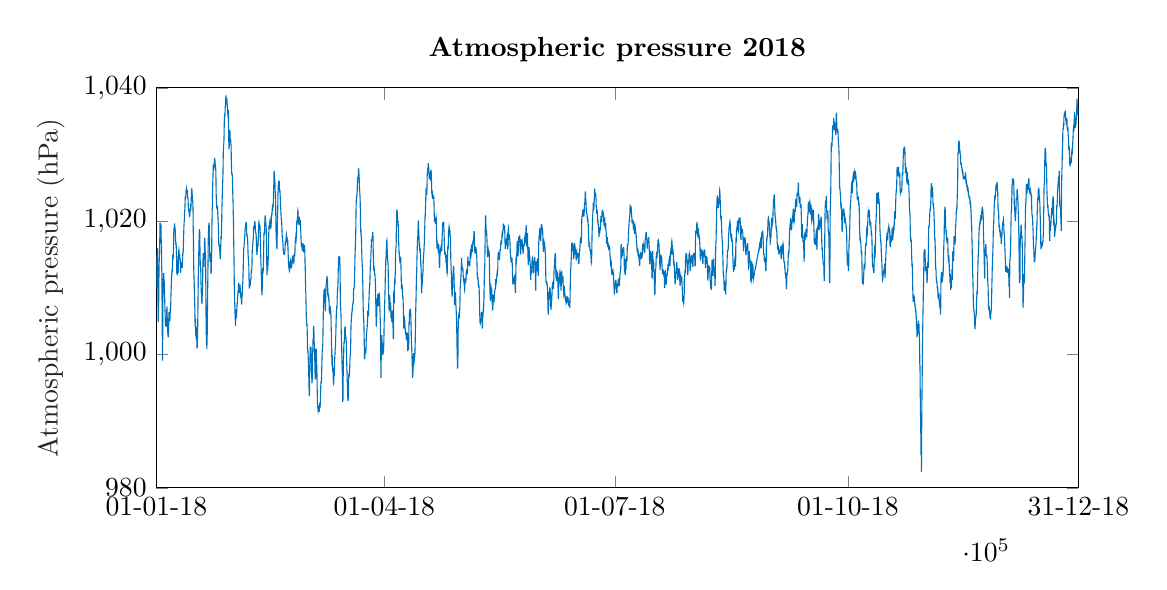
\begin{tikzpicture}

\begin{axis}[%
width=4.61in,
height=2in,
at={(0.758in,0.481in)},
scale only axis,
xmin=737061,
xmax=737425,
xtick={736969,737061,737151,737242,737334,737425},
xticklabels={{01-10-17},{01-01-18},{01-04-18},{01-07-18},{01-10-18},{31-12-18}},
ymin=980,
ymax=1040,
ylabel style={font=\color{white!15!black}},
ylabel={Atmospheric pressure (hPa)},
axis background/.style={fill=white},
title style={font=\bfseries},
title={Atmospheric pressure 2018},
legend style={legend cell align=left, align=left, draw=white!15!black}
]
\addplot [color=mycolor1, forget plot]
  table[row sep=crcr]{%
737061	1010.3\\
737061.034722222	1010\\
737061.069444444	1010.4\\
737061.104166667	1011.3\\
737061.138888889	1012.7\\
737061.173611111	1014.2\\
737061.208333333	1014.8\\
737061.243055556	1014.8\\
737061.277777778	1014.8\\
737061.3125	1014.4\\
737061.347222222	1015\\
737061.381944444	1015.8\\
737061.416666667	1016\\
737061.451388889	1015.7\\
737061.486111111	1014.6\\
737061.520833333	1013.3\\
737061.555555556	1011.6\\
737061.590277778	1009.9\\
737061.625	1008\\
737061.659722222	1007.2\\
737061.694444444	1006.1\\
737061.729166667	1005.6\\
737061.763888889	1004.9\\
737061.798611111	1006.2\\
737061.833333333	1006.9\\
737061.868055556	1007.4\\
737061.902777778	1007.5\\
737061.9375	1008.6\\
737061.972222222	1009.1\\
737062.006944444	1011.5\\
737062.041666667	1012.5\\
737062.076388889	1013\\
737062.111111111	1014\\
737062.145833333	1014.4\\
737062.184027778	1014.8\\
737062.21875	1015.1\\
737062.253472222	1015.6\\
737062.288194444	1016.1\\
737062.322916667	1016.9\\
737062.357638889	1017.6\\
737062.392361111	1018.7\\
737062.427083333	1019.6\\
737062.461805556	1019.8\\
737062.496527778	1019.6\\
737062.53125	1019.5\\
737062.565972222	1019.3\\
737062.600694444	1018.8\\
737062.635416667	1019.6\\
737062.670138889	1019.6\\
737062.704861111	1019.5\\
737062.739583333	1018.8\\
737062.774305556	1018.4\\
737062.809027778	1019.4\\
737062.84375	1019.1\\
737062.878472222	1017.8\\
737062.913194444	1017\\
737062.947916667	1016.7\\
737062.982638889	1016.8\\
737063.017361111	1015.7\\
737063.052083333	1014.7\\
737063.086805556	1013.3\\
737063.121527778	1012.9\\
737063.15625	1012.3\\
737063.190972222	1010.2\\
737063.225694444	1009.1\\
737063.260416667	1006\\
737063.295138889	1004.2\\
737063.329861111	1003.1\\
737063.364583333	1001.4\\
737063.399305556	999.7\\
737063.434027778	999.1\\
737063.46875	1000.6\\
737063.503472222	1003\\
737063.538194444	1007.1\\
737063.572916667	1008.4\\
737063.607638889	1009\\
737063.642361111	1010.3\\
737063.677083333	1011.5\\
737063.711805556	1011.4\\
737063.746527778	1010.8\\
737063.78125	1010.9\\
737063.815972222	1012.2\\
737063.850694444	1012\\
737063.885416667	1011.6\\
737063.920138889	1011.3\\
737063.954861111	1012.2\\
737063.989583333	1011.1\\
737064.027777778	1011.2\\
737064.0625	1011.1\\
737064.097222222	1010.8\\
737064.131944444	1010.2\\
737064.166666667	1009.7\\
737064.201388889	1009.6\\
737064.236111111	1009\\
737064.270833333	1008.5\\
737064.305555556	1008.2\\
737064.34375	1007.3\\
737064.378472222	1006.8\\
737064.413194444	1006.5\\
737064.447916667	1006\\
737064.482638889	1005.5\\
737064.517361111	1005\\
737064.552083333	1004.6\\
737064.586805556	1004.7\\
737064.621527778	1004.3\\
737064.65625	1004.7\\
737064.690972222	1004.7\\
737064.725694444	1004.6\\
737064.760416667	1004.6\\
737064.795138889	1004.6\\
737064.829861111	1004.1\\
737064.864583333	1004.4\\
737064.899305556	1004.7\\
737064.934027778	1004.9\\
737064.96875	1004.5\\
737065.003472222	1004.6\\
737065.038194444	1005.1\\
737065.072916667	1005.9\\
737065.107638889	1006.7\\
737065.142361111	1007.1\\
737065.177083333	1007.1\\
737065.211805556	1006.4\\
737065.246527778	1005.8\\
737065.28125	1005.6\\
737065.315972222	1005.1\\
737065.350694444	1004.4\\
737065.385416667	1004.4\\
737065.420138889	1004.1\\
737065.454861111	1003.8\\
737065.489583333	1003.5\\
737065.524305556	1003\\
737065.559027778	1002.8\\
737065.59375	1002.8\\
737065.628472222	1003.1\\
737065.663194444	1002.7\\
737065.697916667	1002.6\\
737065.732638889	1002.9\\
737065.767361111	1003.3\\
737065.802083333	1003.8\\
737065.836805556	1004.1\\
737065.871527778	1004.8\\
737065.90625	1005.5\\
737065.940972222	1006.1\\
737065.975694444	1006.4\\
737066.013888889	1006.3\\
737066.048611111	1006.3\\
737066.083333333	1006.3\\
737066.118055556	1006.3\\
737066.152777778	1006\\
737066.1875	1005.7\\
737066.222222222	1005.5\\
737066.256944444	1005.4\\
737066.291666667	1005.2\\
737066.326388889	1005\\
737066.361111111	1005.5\\
737066.395833333	1006.3\\
737066.430555556	1006.9\\
737066.465277778	1006.9\\
737066.5	1006.8\\
737066.534722222	1006.7\\
737066.569444444	1006.6\\
737066.604166667	1006.7\\
737066.638888889	1007.2\\
737066.673611111	1007.7\\
737066.708333333	1008.2\\
737066.743055556	1008.7\\
737066.777777778	1009.2\\
737066.8125	1009.4\\
737066.847222222	1009.9\\
737066.881944444	1010.3\\
737066.916666667	1010.8\\
737066.951388889	1011.1\\
737066.986111111	1011.7\\
737067.024305556	1011.9\\
737067.059027778	1011.9\\
737067.09375	1012.2\\
737067.128472222	1012.5\\
737067.163194444	1012.6\\
737067.201388889	1012.5\\
737067.236111111	1012.4\\
737067.270833333	1012.4\\
737067.305555556	1012.8\\
737067.340277778	1013.3\\
737067.375	1014\\
737067.409722222	1014.5\\
737067.444444444	1014.9\\
737067.479166667	1014.7\\
737067.513888889	1014.5\\
737067.548611111	1014.3\\
737067.583333333	1014.3\\
737067.618055556	1014.3\\
737067.652777778	1014.8\\
737067.6875	1015.2\\
737067.722222222	1015.6\\
737067.756944444	1016.2\\
737067.791666667	1017.1\\
737067.826388889	1017.6\\
737067.861111111	1018.2\\
737067.895833333	1018.7\\
737067.930555556	1018.8\\
737067.965277778	1019\\
737068	1018.9\\
737068.034722222	1018.9\\
737068.069444444	1018.6\\
737068.104166667	1019\\
737068.138888889	1019.4\\
737068.173611111	1019.6\\
737068.208333333	1019.6\\
737068.243055556	1019.1\\
737068.277777778	1019.1\\
737068.3125	1019.2\\
737068.347222222	1018.9\\
737068.381944444	1018.7\\
737068.416666667	1018.6\\
737068.451388889	1018.6\\
737068.486111111	1018.4\\
737068.520833333	1017.7\\
737068.555555556	1017.2\\
737068.590277778	1016.6\\
737068.625	1016.6\\
737068.659722222	1016.7\\
737068.694444444	1016.9\\
737068.729166667	1016.8\\
737068.763888889	1016.5\\
737068.798611111	1016.4\\
737068.833333333	1016.3\\
737068.868055556	1015.9\\
737068.902777778	1015.7\\
737068.9375	1014.7\\
737068.972222222	1014\\
737069.010416667	1013\\
737069.045138889	1012.5\\
737069.079861111	1012\\
737069.114583333	1012.3\\
737069.149305556	1013.7\\
737069.1875	1014.8\\
737069.222222222	1013.9\\
737069.256944444	1014\\
737069.291666667	1013.6\\
737069.326388889	1013.8\\
737069.361111111	1012.5\\
737069.395833333	1012.9\\
737069.430555556	1012.5\\
737069.465277778	1012.4\\
737069.5	1012.5\\
737069.534722222	1012.4\\
737069.569444444	1012.4\\
737069.604166667	1012.6\\
737069.638888889	1012.3\\
737069.673611111	1012.7\\
737069.708333333	1013.6\\
737069.743055556	1014\\
737069.777777778	1014.7\\
737069.8125	1015.4\\
737069.847222222	1015.6\\
737069.881944444	1015.7\\
737069.916666667	1015.6\\
737069.951388889	1015.3\\
737069.986111111	1014.7\\
737070.020833333	1014.6\\
737070.055555556	1014.4\\
737070.090277778	1014.5\\
737070.125	1014.7\\
737070.159722222	1015\\
737070.197916667	1015\\
737070.232638889	1014.7\\
737070.267361111	1014.5\\
737070.302083333	1014.4\\
737070.336805556	1014.3\\
737070.371527778	1014.3\\
737070.40625	1014.2\\
737070.440972222	1014.2\\
737070.475694444	1013.5\\
737070.510416667	1013\\
737070.545138889	1012.5\\
737070.579861111	1012.2\\
737070.614583333	1012.6\\
737070.649305556	1013\\
737070.684027778	1013.2\\
737070.71875	1013.1\\
737070.753472222	1013.1\\
737070.788194444	1013.5\\
737070.822916667	1013.7\\
737070.857638889	1013.6\\
737070.892361111	1013.6\\
737070.927083333	1013.5\\
737070.961805556	1013.8\\
737070.996527778	1013.7\\
737071.03125	1013.5\\
737071.065972222	1013.2\\
737071.100694444	1013.1\\
737071.135416667	1013.3\\
737071.173611111	1013.2\\
737071.208333333	1013\\
737071.243055556	1013.3\\
737071.277777778	1013.6\\
737071.3125	1014\\
737071.347222222	1014.3\\
737071.381944444	1014.8\\
737071.416666667	1015.1\\
737071.451388889	1015.3\\
737071.486111111	1015.3\\
737071.520833333	1015.3\\
737071.555555556	1015.2\\
737071.590277778	1015.5\\
737071.625	1015.9\\
737071.659722222	1016.4\\
737071.694444444	1016.9\\
737071.729166667	1017.3\\
737071.763888889	1017.8\\
737071.798611111	1018.3\\
737071.833333333	1018.7\\
737071.868055556	1019.2\\
737071.902777778	1019.4\\
737071.9375	1019.6\\
737071.972222222	1019.9\\
737072.006944444	1020.1\\
737072.041666667	1020.4\\
737072.076388889	1020.8\\
737072.111111111	1021.2\\
737072.145833333	1021.3\\
737072.184027778	1021.5\\
737072.21875	1021.7\\
737072.253472222	1021.9\\
737072.288194444	1022.2\\
737072.322916667	1022.7\\
737072.357638889	1023\\
737072.392361111	1023.3\\
737072.427083333	1023.8\\
737072.461805556	1023.8\\
737072.496527778	1023.8\\
737072.53125	1023.6\\
737072.565972222	1023.6\\
737072.600694444	1023.6\\
737072.635416667	1023.8\\
737072.670138889	1024.2\\
737072.704861111	1024.5\\
737072.739583333	1024.5\\
737072.774305556	1024.5\\
737072.809027778	1024.8\\
737072.84375	1024.8\\
737072.878472222	1024.9\\
737072.913194444	1024.8\\
737072.947916667	1024.8\\
737072.982638889	1024.6\\
737073.017361111	1024.4\\
737073.052083333	1024.3\\
737073.086805556	1024.2\\
737073.121527778	1024.6\\
737073.15625	1024.7\\
737073.194444444	1024.4\\
737073.229166667	1024.2\\
737073.263888889	1024\\
737073.298611111	1024\\
737073.333333333	1023.7\\
737073.368055556	1023.6\\
737073.402777778	1023.6\\
737073.4375	1023.6\\
737073.472222222	1023.5\\
737073.506944444	1023.3\\
737073.541666667	1022.9\\
737073.576388889	1022.5\\
737073.611111111	1022.2\\
737073.645833333	1022\\
737073.680555556	1021.7\\
737073.715277778	1021.7\\
737073.75	1021.7\\
737073.784722222	1021.6\\
737073.819444444	1021.6\\
737073.854166667	1021.6\\
737073.888888889	1021.4\\
737073.923611111	1021.3\\
737073.958333333	1021.2\\
737073.993055556	1021\\
737074.027777778	1020.9\\
737074.0625	1020.8\\
737074.097222222	1020.8\\
737074.131944444	1020.6\\
737074.166666667	1020.9\\
737074.204861111	1020.9\\
737074.239583333	1021.2\\
737074.274305556	1021.4\\
737074.309027778	1021.6\\
737074.34375	1021.8\\
737074.378472222	1021.9\\
737074.413194444	1022.1\\
737074.447916667	1022.6\\
737074.482638889	1022.4\\
737074.517361111	1021.9\\
737074.552083333	1021.6\\
737074.586805556	1021.7\\
737074.621527778	1021.9\\
737074.65625	1022.3\\
737074.690972222	1022.7\\
737074.725694444	1022.9\\
737074.760416667	1023.2\\
737074.795138889	1023.8\\
737074.829861111	1024.1\\
737074.864583333	1024.2\\
737074.899305556	1024.4\\
737074.934027778	1024.5\\
737074.96875	1024.7\\
737075.003472222	1025\\
737075.038194444	1024.6\\
737075.072916667	1024.2\\
737075.107638889	1024.3\\
737075.142361111	1024\\
737075.177083333	1023.9\\
737075.211805556	1023.4\\
737075.246527778	1023.3\\
737075.28125	1023\\
737075.315972222	1023\\
737075.350694444	1023\\
737075.385416667	1022.7\\
737075.420138889	1022.3\\
737075.454861111	1021.9\\
737075.489583333	1021\\
737075.524305556	1019.4\\
737075.559027778	1018.6\\
737075.59375	1017.7\\
737075.628472222	1017.1\\
737075.663194444	1015.9\\
737075.697916667	1014.4\\
737075.732638889	1013.4\\
737075.767361111	1012.6\\
737075.802083333	1012.5\\
737075.836805556	1011.8\\
737075.871527778	1011.3\\
737075.90625	1011\\
737075.940972222	1010.5\\
737075.975694444	1009.7\\
737076.013888889	1009\\
737076.048611111	1008.2\\
737076.083333333	1007.9\\
737076.118055556	1007.8\\
737076.152777778	1007.5\\
737076.190972222	1006.5\\
737076.225694444	1006\\
737076.260416667	1004.9\\
737076.295138889	1004.8\\
737076.329861111	1004.1\\
737076.364583333	1005.1\\
737076.399305556	1005.3\\
737076.434027778	1005.3\\
737076.46875	1004.5\\
737076.503472222	1003.7\\
737076.538194444	1003.4\\
737076.572916667	1002.7\\
737076.607638889	1002.9\\
737076.642361111	1003.2\\
737076.677083333	1004.1\\
737076.711805556	1003.9\\
737076.746527778	1002.5\\
737076.78125	1004.1\\
737076.815972222	1003.2\\
737076.850694444	1002.1\\
737076.885416667	1002.9\\
737076.920138889	1003.3\\
737076.954861111	1002.9\\
737076.989583333	1002.7\\
737077.024305556	1001.7\\
737077.059027778	1000.9\\
737077.09375	1001.5\\
737077.128472222	1001.2\\
737077.163194444	1001.1\\
737077.197916667	1002.3\\
737077.232638889	1002.4\\
737077.267361111	1003.6\\
737077.302083333	1003.9\\
737077.336805556	1004.9\\
737077.371527778	1005.9\\
737077.40625	1006.7\\
737077.440972222	1008.4\\
737077.475694444	1009.6\\
737077.510416667	1010.1\\
737077.545138889	1011.7\\
737077.579861111	1012.7\\
737077.614583333	1013.1\\
737077.649305556	1013.8\\
737077.684027778	1014.6\\
737077.71875	1015\\
737077.753472222	1015.6\\
737077.788194444	1016.3\\
737077.822916667	1016.8\\
737077.857638889	1017.3\\
737077.892361111	1018.1\\
737077.927083333	1018.3\\
737077.961805556	1017.8\\
737078	1018.7\\
737078.034722222	1018.8\\
737078.069444444	1018.3\\
737078.104166667	1018.4\\
737078.138888889	1017.9\\
737078.173611111	1016.8\\
737078.208333333	1015.9\\
737078.243055556	1015.4\\
737078.277777778	1014.5\\
737078.3125	1013.7\\
737078.347222222	1013.3\\
737078.381944444	1013.4\\
737078.416666667	1013.2\\
737078.451388889	1012.9\\
737078.486111111	1013.2\\
737078.520833333	1012.6\\
737078.555555556	1012.1\\
737078.590277778	1011.1\\
737078.625	1010.6\\
737078.659722222	1010\\
737078.694444444	1009.4\\
737078.729166667	1009.4\\
737078.763888889	1009.6\\
737078.798611111	1009.4\\
737078.833333333	1008.9\\
737078.868055556	1008.2\\
737078.902777778	1008.3\\
737078.9375	1007.7\\
737078.972222222	1007.6\\
737079.010416667	1007.9\\
737079.045138889	1008\\
737079.079861111	1008.6\\
737079.114583333	1009.8\\
737079.149305556	1009.8\\
737079.1875	1009.6\\
737079.222222222	1009.7\\
737079.256944444	1010.6\\
737079.291666667	1012\\
737079.326388889	1012.9\\
737079.361111111	1013.6\\
737079.395833333	1014.1\\
737079.430555556	1014.4\\
737079.465277778	1015.1\\
737079.5	1015.2\\
737079.534722222	1014.5\\
737079.569444444	1013.8\\
737079.604166667	1013.5\\
737079.638888889	1013.5\\
737079.673611111	1013.3\\
737079.708333333	1013.2\\
737079.743055556	1013.2\\
737079.777777778	1013.2\\
737079.8125	1013.3\\
737079.847222222	1013.9\\
737079.881944444	1014.5\\
737079.916666667	1015.2\\
737079.951388889	1015.9\\
737079.986111111	1016.4\\
737080.020833333	1017\\
737080.055555556	1017.1\\
737080.090277778	1017.5\\
737080.125	1017.4\\
737080.159722222	1016.9\\
737080.197916667	1016.5\\
737080.232638889	1015.9\\
737080.267361111	1015.5\\
737080.302083333	1015.2\\
737080.336805556	1014.9\\
737080.371527778	1014.9\\
737080.40625	1014.4\\
737080.440972222	1013.7\\
737080.475694444	1012.6\\
737080.510416667	1010.7\\
737080.545138889	1008.6\\
737080.579861111	1006.6\\
737080.614583333	1005.4\\
737080.649305556	1004.3\\
737080.684027778	1003.7\\
737080.71875	1002.5\\
737080.753472222	1001.8\\
737080.788194444	1001.7\\
737080.822916667	1001.4\\
737080.857638889	1001.7\\
737080.892361111	1001.6\\
737080.927083333	1000.8\\
737080.961805556	1001.5\\
737080.996527778	1001.4\\
737081.03125	1002.1\\
737081.065972222	1003.1\\
737081.100694444	1004.4\\
737081.135416667	1005.8\\
737081.170138889	1007.1\\
737081.204861111	1008.5\\
737081.239583333	1009.3\\
737081.274305556	1010.5\\
737081.309027778	1011.2\\
737081.34375	1012.5\\
737081.378472222	1013.7\\
737081.413194444	1014.7\\
737081.447916667	1016.1\\
737081.482638889	1017.2\\
737081.517361111	1017.8\\
737081.552083333	1018.2\\
737081.586805556	1018.5\\
737081.621527778	1018.9\\
737081.65625	1019.2\\
737081.690972222	1019.4\\
737081.725694444	1019.6\\
737081.760416667	1019.6\\
737081.795138889	1019.7\\
737081.829861111	1019.7\\
737081.864583333	1019.1\\
737081.899305556	1018.8\\
737081.934027778	1017.9\\
737081.96875	1017.4\\
737082.006944444	1016.6\\
737082.041666667	1015.6\\
737082.076388889	1014.7\\
737082.111111111	1014.3\\
737082.145833333	1013.9\\
737082.180555556	1014.2\\
737082.215277778	1014.5\\
737082.25	1014.8\\
737082.284722222	1014.8\\
737082.319444444	1014.9\\
737082.354166667	1014.9\\
737082.388888889	1014.6\\
737082.423611111	1014.7\\
737082.458333333	1015.2\\
737082.493055556	1015\\
737082.527777778	1013.5\\
737082.5625	1012.2\\
737082.597222222	1012.1\\
737082.631944444	1012.3\\
737082.666666667	1012.6\\
737082.701388889	1013.3\\
737082.736111111	1013.9\\
737082.770833333	1014.1\\
737082.805555556	1014.6\\
737082.840277778	1015.5\\
737082.875	1017.3\\
737082.909722222	1018.6\\
737082.944444444	1019.7\\
737082.979166667	1020.5\\
737083.017361111	1021.5\\
737083.052083333	1021.9\\
737083.086805556	1022.1\\
737083.121527778	1023.1\\
737083.15625	1023.9\\
737083.190972222	1024.5\\
737083.225694444	1025.2\\
737083.260416667	1025.8\\
737083.295138889	1025.9\\
737083.329861111	1026.5\\
737083.364583333	1027.2\\
737083.399305556	1027.5\\
737083.434027778	1028\\
737083.46875	1028.5\\
737083.503472222	1028.3\\
737083.538194444	1028.3\\
737083.572916667	1028.1\\
737083.607638889	1027.9\\
737083.642361111	1027.7\\
737083.677083333	1027.7\\
737083.711805556	1028\\
737083.746527778	1028.2\\
737083.78125	1028.2\\
737083.815972222	1028.2\\
737083.850694444	1028.7\\
737083.885416667	1029.1\\
737083.920138889	1029.3\\
737083.954861111	1029\\
737083.989583333	1029.1\\
737084.027777778	1029.4\\
737084.0625	1029.4\\
737084.097222222	1029.2\\
737084.131944444	1029\\
737084.166666667	1028.5\\
737084.204861111	1028.4\\
737084.239583333	1028.5\\
737084.274305556	1028.6\\
737084.309027778	1028.4\\
737084.34375	1028.2\\
737084.378472222	1028\\
737084.413194444	1027.9\\
737084.447916667	1027.8\\
737084.482638889	1027.1\\
737084.517361111	1026.4\\
737084.552083333	1025.3\\
737084.586805556	1024.6\\
737084.621527778	1023.8\\
737084.65625	1023.5\\
737084.690972222	1023.1\\
737084.725694444	1022.8\\
737084.760416667	1022.3\\
737084.795138889	1022.4\\
737084.829861111	1022.3\\
737084.864583333	1021.9\\
737084.899305556	1021.8\\
737084.934027778	1022\\
737084.96875	1022.3\\
737085.003472222	1022.1\\
737085.038194444	1022.3\\
737085.072916667	1022\\
737085.107638889	1022\\
737085.142361111	1021.8\\
737085.180555556	1021.5\\
737085.215277778	1021.4\\
737085.25	1021\\
737085.284722222	1020.8\\
737085.319444444	1020.5\\
737085.354166667	1020.1\\
737085.388888889	1019.8\\
737085.423611111	1019.7\\
737085.458333333	1019.6\\
737085.493055556	1019.3\\
737085.527777778	1018.7\\
737085.5625	1017.9\\
737085.597222222	1017.1\\
737085.631944444	1016.6\\
737085.666666667	1016.5\\
737085.701388889	1016.5\\
737085.736111111	1016.3\\
737085.770833333	1016.4\\
737085.805555556	1016.4\\
737085.840277778	1016.2\\
737085.875	1016.3\\
737085.909722222	1016.4\\
737085.944444444	1016.4\\
737085.979166667	1016.2\\
737086.013888889	1015.7\\
737086.048611111	1015.4\\
737086.083333333	1015.3\\
737086.118055556	1015.1\\
737086.152777778	1014.6\\
737086.190972222	1014.3\\
737086.225694444	1014.7\\
737086.260416667	1014.7\\
737086.295138889	1015.1\\
737086.329861111	1015.6\\
737086.364583333	1016\\
737086.399305556	1016\\
737086.434027778	1016.6\\
737086.46875	1017.2\\
737086.506944444	1017.6\\
737086.541666667	1017.6\\
737086.576388889	1017.3\\
737086.611111111	1017.5\\
737086.645833333	1018\\
737086.680555556	1018.2\\
737086.715277778	1018.6\\
737086.75	1019.3\\
737086.784722222	1020\\
737086.819444444	1020.9\\
737086.854166667	1021.6\\
737086.888888889	1022.3\\
737086.923611111	1022.6\\
737086.958333333	1022.9\\
737086.993055556	1023.6\\
737087.027777778	1024.1\\
737087.0625	1024.5\\
737087.097222222	1025\\
737087.131944444	1025.4\\
737087.166666667	1025.7\\
737087.204861111	1026.1\\
737087.239583333	1026.5\\
737087.274305556	1026.9\\
737087.309027778	1027.8\\
737087.34375	1028.7\\
737087.378472222	1029.4\\
737087.413194444	1030.4\\
737087.447916667	1030.6\\
737087.482638889	1030.7\\
737087.517361111	1030.6\\
737087.552083333	1031.3\\
737087.586805556	1031.6\\
737087.621527778	1031.6\\
737087.65625	1032\\
737087.690972222	1032.4\\
737087.725694444	1033\\
737087.760416667	1033.8\\
737087.795138889	1034.7\\
737087.829861111	1035.2\\
737087.864583333	1035.3\\
737087.899305556	1035.8\\
737087.934027778	1035.9\\
737087.96875	1036\\
737088.003472222	1035.7\\
737088.038194444	1035.9\\
737088.072916667	1035.9\\
737088.107638889	1036.3\\
737088.142361111	1036.6\\
737088.180555556	1037.2\\
737088.215277778	1037.3\\
737088.25	1037.4\\
737088.284722222	1037.7\\
737088.319444444	1037.8\\
737088.354166667	1038.3\\
737088.388888889	1038.3\\
737088.423611111	1038.7\\
737088.458333333	1038.8\\
737088.493055556	1038.8\\
737088.527777778	1038.8\\
737088.5625	1038.4\\
737088.597222222	1037.9\\
737088.631944444	1037.6\\
737088.666666667	1037.6\\
737088.701388889	1037.5\\
737088.736111111	1037.9\\
737088.770833333	1038.4\\
737088.805555556	1038.4\\
737088.840277778	1038.3\\
737088.875	1038.1\\
737088.909722222	1038.1\\
737088.944444444	1037.7\\
737088.979166667	1037.3\\
737089.013888889	1037.1\\
737089.048611111	1037\\
737089.083333333	1036.9\\
737089.118055556	1036.6\\
737089.152777778	1036.4\\
737089.190972222	1036.5\\
737089.225694444	1036.5\\
737089.260416667	1036.6\\
737089.295138889	1036.4\\
737089.329861111	1036.6\\
737089.364583333	1036.7\\
737089.399305556	1036.4\\
737089.434027778	1035.9\\
737089.46875	1035.5\\
737089.503472222	1034.4\\
737089.538194444	1033.2\\
737089.572916667	1032.2\\
737089.607638889	1031.6\\
737089.642361111	1031\\
737089.677083333	1030.8\\
737089.711805556	1031.1\\
737089.746527778	1031.3\\
737089.78125	1031.9\\
737089.815972222	1032.8\\
737089.850694444	1033.1\\
737089.885416667	1033.1\\
737089.920138889	1033.1\\
737089.954861111	1033.4\\
737089.989583333	1033.5\\
737090.024305556	1033.7\\
737090.059027778	1033.1\\
737090.09375	1032.6\\
737090.128472222	1032.5\\
737090.163194444	1032.3\\
737090.197916667	1032.3\\
737090.232638889	1032.2\\
737090.267361111	1032.3\\
737090.302083333	1032.4\\
737090.336805556	1032.1\\
737090.371527778	1031.9\\
737090.40625	1031.8\\
737090.440972222	1031.5\\
737090.475694444	1031.4\\
737090.510416667	1030.8\\
737090.545138889	1030.1\\
737090.579861111	1029.2\\
737090.614583333	1028.6\\
737090.649305556	1028.3\\
737090.684027778	1027.9\\
737090.71875	1027.4\\
737090.753472222	1027.1\\
737090.788194444	1027.1\\
737090.822916667	1027.1\\
737090.857638889	1027.2\\
737090.892361111	1027.2\\
737090.927083333	1027\\
737090.961805556	1026.9\\
737091	1026.4\\
737091.034722222	1026.1\\
737091.069444444	1025.6\\
737091.104166667	1025.3\\
737091.138888889	1024.7\\
737091.173611111	1023.9\\
737091.208333333	1023.5\\
737091.243055556	1023.1\\
737091.277777778	1022.6\\
737091.3125	1021.8\\
737091.347222222	1021.2\\
737091.381944444	1020.6\\
737091.416666667	1020.3\\
737091.451388889	1019.7\\
737091.486111111	1018.7\\
737091.520833333	1017.4\\
737091.555555556	1016.4\\
737091.590277778	1015.5\\
737091.625	1014.6\\
737091.659722222	1013.4\\
737091.694444444	1012.5\\
737091.729166667	1011.4\\
737091.763888889	1010.4\\
737091.798611111	1009.5\\
737091.833333333	1009\\
737091.868055556	1008.6\\
737091.902777778	1008.1\\
737091.9375	1007.6\\
737091.972222222	1006.9\\
737092.010416667	1006.8\\
737092.045138889	1006.1\\
737092.079861111	1005.8\\
737092.114583333	1005.9\\
737092.149305556	1005.3\\
737092.184027778	1004.8\\
737092.21875	1004.8\\
737092.253472222	1004.4\\
737092.288194444	1004.4\\
737092.322916667	1005.3\\
737092.357638889	1005.6\\
737092.392361111	1006\\
737092.427083333	1006.4\\
737092.461805556	1006.8\\
737092.496527778	1006.3\\
737092.53125	1005.9\\
737092.565972222	1005.8\\
737092.600694444	1005.5\\
737092.635416667	1005.8\\
737092.670138889	1006.2\\
737092.704861111	1006.4\\
737092.739583333	1006.4\\
737092.774305556	1006.9\\
737092.809027778	1007.1\\
737092.84375	1007.6\\
737092.878472222	1007.7\\
737092.913194444	1007.7\\
737092.947916667	1007.7\\
737092.982638889	1007.9\\
737093.020833333	1008.5\\
737093.055555556	1008.4\\
737093.090277778	1008.6\\
737093.125	1009\\
737093.159722222	1009.1\\
737093.197916667	1009.3\\
737093.232638889	1009.6\\
737093.267361111	1009.4\\
737093.302083333	1009.3\\
737093.336805556	1009.5\\
737093.371527778	1010\\
737093.40625	1010.4\\
737093.440972222	1010.6\\
737093.475694444	1010.8\\
737093.510416667	1010\\
737093.545138889	1009.8\\
737093.579861111	1009.5\\
737093.614583333	1009.2\\
737093.649305556	1009.7\\
737093.684027778	1009.8\\
737093.71875	1009.7\\
737093.753472222	1009.7\\
737093.788194444	1010.1\\
737093.822916667	1010.3\\
737093.857638889	1010.2\\
737093.892361111	1010.3\\
737093.927083333	1010.5\\
737093.961805556	1010.4\\
737093.996527778	1010.5\\
737094.03125	1010.2\\
737094.065972222	1010.1\\
737094.100694444	1010\\
737094.135416667	1009.3\\
737094.173611111	1009\\
737094.208333333	1009\\
737094.243055556	1008.7\\
737094.277777778	1008.6\\
737094.3125	1008.8\\
737094.347222222	1008.9\\
737094.381944444	1009\\
737094.416666667	1008.9\\
737094.451388889	1008.9\\
737094.486111111	1008.8\\
737094.520833333	1008.3\\
737094.555555556	1008.1\\
737094.590277778	1007.8\\
737094.625	1007.6\\
737094.659722222	1007.5\\
737094.694444444	1007.8\\
737094.729166667	1008\\
737094.763888889	1008.4\\
737094.798611111	1008.7\\
737094.833333333	1008.8\\
737094.868055556	1008.9\\
737094.902777778	1009.1\\
737094.9375	1009.5\\
737094.972222222	1010\\
737095.006944444	1010.4\\
737095.041666667	1010.7\\
737095.076388889	1010.7\\
737095.111111111	1010.9\\
737095.145833333	1011\\
737095.184027778	1011.6\\
737095.21875	1012.3\\
737095.253472222	1012.5\\
737095.288194444	1012.8\\
737095.322916667	1013.8\\
737095.357638889	1014.5\\
737095.392361111	1014.8\\
737095.427083333	1015.1\\
737095.461805556	1015.7\\
737095.496527778	1016\\
737095.53125	1015.9\\
737095.565972222	1016.1\\
737095.600694444	1016.2\\
737095.635416667	1016.2\\
737095.670138889	1016.6\\
737095.704861111	1016.8\\
737095.739583333	1016.8\\
737095.774305556	1017.1\\
737095.809027778	1017.4\\
737095.84375	1017.5\\
737095.878472222	1017.7\\
737095.913194444	1018\\
737095.947916667	1018.3\\
737095.982638889	1018.5\\
737096.017361111	1018.7\\
737096.052083333	1018.7\\
737096.086805556	1019\\
737096.121527778	1019\\
737096.15625	1018.8\\
737096.190972222	1019.1\\
737096.225694444	1019.4\\
737096.260416667	1019.6\\
737096.295138889	1019.5\\
737096.329861111	1019.6\\
737096.364583333	1019.9\\
737096.399305556	1019.7\\
737096.434027778	1019.6\\
737096.46875	1019.8\\
737096.503472222	1019.4\\
737096.538194444	1019.6\\
737096.572916667	1019.6\\
737096.607638889	1018.9\\
737096.642361111	1018.3\\
737096.677083333	1017.9\\
737096.711805556	1017.8\\
737096.746527778	1018\\
737096.78125	1018\\
737096.815972222	1017.8\\
737096.850694444	1017.8\\
737096.885416667	1017.7\\
737096.920138889	1017.8\\
737096.954861111	1017.5\\
737096.989583333	1017.1\\
737097.027777778	1017\\
737097.0625	1016.7\\
737097.097222222	1016.4\\
737097.131944444	1015.9\\
737097.166666667	1015.4\\
737097.204861111	1015\\
737097.239583333	1014.8\\
737097.274305556	1014.7\\
737097.309027778	1014.3\\
737097.34375	1014.2\\
737097.378472222	1014.1\\
737097.413194444	1013.7\\
737097.447916667	1013.5\\
737097.482638889	1013.4\\
737097.517361111	1012.8\\
737097.552083333	1012\\
737097.586805556	1011.1\\
737097.621527778	1010.6\\
737097.65625	1010.3\\
737097.690972222	1010\\
737097.725694444	1009.9\\
737097.760416667	1010.1\\
737097.795138889	1010.3\\
737097.829861111	1010.3\\
737097.864583333	1010.3\\
737097.899305556	1010.4\\
737097.934027778	1010.4\\
737097.96875	1010.3\\
737098.003472222	1010.3\\
737098.038194444	1010.4\\
737098.072916667	1010.6\\
737098.107638889	1011\\
737098.142361111	1011\\
737098.180555556	1011.2\\
737098.215277778	1011.2\\
737098.25	1011.3\\
737098.284722222	1011.1\\
737098.319444444	1011.3\\
737098.354166667	1011.4\\
737098.388888889	1011.6\\
737098.423611111	1012.1\\
737098.458333333	1012.5\\
737098.493055556	1012.6\\
737098.527777778	1012.6\\
737098.5625	1012.4\\
737098.597222222	1012.7\\
737098.631944444	1012.7\\
737098.666666667	1012.8\\
737098.701388889	1013.2\\
737098.736111111	1013.6\\
737098.770833333	1014.5\\
737098.805555556	1015\\
737098.840277778	1015.4\\
737098.875	1015.8\\
737098.909722222	1015.9\\
737098.944444444	1016.1\\
737098.979166667	1016.2\\
737099.013888889	1016.3\\
737099.048611111	1016.5\\
737099.083333333	1016.8\\
737099.118055556	1017.1\\
737099.152777778	1017\\
737099.190972222	1017.1\\
737099.225694444	1017.3\\
737099.260416667	1017.5\\
737099.295138889	1017.9\\
737099.329861111	1018.4\\
737099.364583333	1018.9\\
737099.399305556	1019.1\\
737099.434027778	1019.1\\
737099.46875	1019.3\\
737099.503472222	1019.2\\
737099.538194444	1019.2\\
737099.572916667	1019.1\\
737099.607638889	1018.8\\
737099.642361111	1019\\
737099.677083333	1019\\
737099.711805556	1019.3\\
737099.746527778	1019.6\\
737099.78125	1019.7\\
737099.815972222	1019.8\\
737099.850694444	1019.8\\
737099.885416667	1020\\
737099.920138889	1019.9\\
737099.954861111	1019.7\\
737099.989583333	1019.5\\
737100.024305556	1019.3\\
737100.059027778	1019.1\\
737100.09375	1018.9\\
737100.128472222	1018.8\\
737100.163194444	1018.5\\
737100.197916667	1018.3\\
737100.232638889	1018.3\\
737100.267361111	1018.2\\
737100.302083333	1018.1\\
737100.336805556	1018.1\\
737100.371527778	1018\\
737100.40625	1017.7\\
737100.440972222	1017.4\\
737100.475694444	1017\\
737100.510416667	1016.4\\
737100.545138889	1016.1\\
737100.579861111	1015.6\\
737100.614583333	1015.5\\
737100.649305556	1015.3\\
737100.684027778	1015.1\\
737100.71875	1014.9\\
737100.753472222	1015.3\\
737100.788194444	1015.6\\
737100.822916667	1015.6\\
737100.857638889	1015.8\\
737100.892361111	1015.9\\
737100.927083333	1016.1\\
737100.961805556	1016.3\\
737101	1016.2\\
737101.034722222	1016.2\\
737101.069444444	1016.4\\
737101.104166667	1016.4\\
737101.138888889	1016.6\\
737101.177083333	1016.8\\
737101.211805556	1017.2\\
737101.246527778	1017.5\\
737101.28125	1018.2\\
737101.315972222	1018.4\\
737101.350694444	1018.9\\
737101.385416667	1019.2\\
737101.420138889	1019.6\\
737101.454861111	1019.7\\
737101.489583333	1019.8\\
737101.524305556	1019.7\\
737101.559027778	1019.5\\
737101.59375	1019.3\\
737101.628472222	1019.1\\
737101.663194444	1019.2\\
737101.697916667	1019.3\\
737101.732638889	1019.2\\
737101.767361111	1019.3\\
737101.802083333	1019.3\\
737101.836805556	1019.2\\
737101.871527778	1019.4\\
737101.90625	1019.3\\
737101.940972222	1018.9\\
737101.975694444	1018.5\\
737102.010416667	1017.8\\
737102.045138889	1017.1\\
737102.079861111	1016.8\\
737102.114583333	1016.4\\
737102.149305556	1015.5\\
737102.184027778	1014.9\\
737102.21875	1014.5\\
737102.253472222	1014.1\\
737102.288194444	1013.5\\
737102.322916667	1013.4\\
737102.357638889	1012.9\\
737102.392361111	1012.3\\
737102.427083333	1011.9\\
737102.461805556	1011.5\\
737102.496527778	1011.3\\
737102.53125	1010.8\\
737102.565972222	1010.4\\
737102.600694444	1009.7\\
737102.635416667	1009.3\\
737102.670138889	1009\\
737102.704861111	1009\\
737102.739583333	1009.2\\
737102.774305556	1009.8\\
737102.809027778	1010.3\\
737102.84375	1011.1\\
737102.878472222	1011.8\\
737102.913194444	1012.3\\
737102.947916667	1012.6\\
737102.982638889	1013\\
737103.020833333	1012.7\\
737103.055555556	1012.6\\
737103.090277778	1012.3\\
737103.125	1012.2\\
737103.159722222	1012.5\\
737103.197916667	1012.8\\
737103.232638889	1013.3\\
737103.267361111	1013.7\\
737103.302083333	1014.5\\
737103.336805556	1015.5\\
737103.371527778	1016.2\\
737103.40625	1017\\
737103.440972222	1017.5\\
737103.475694444	1018\\
737103.510416667	1018.3\\
737103.545138889	1018.2\\
737103.579861111	1018.2\\
737103.614583333	1018\\
737103.649305556	1018.2\\
737103.684027778	1018.2\\
737103.71875	1018.9\\
737103.753472222	1019.4\\
737103.788194444	1019.7\\
737103.822916667	1020.1\\
737103.857638889	1020.3\\
737103.892361111	1020.6\\
737103.927083333	1020.8\\
737103.961805556	1020.8\\
737103.996527778	1020.8\\
737104.03125	1020.6\\
737104.065972222	1020.4\\
737104.100694444	1020.2\\
737104.135416667	1020\\
737104.170138889	1019.7\\
737104.204861111	1019.6\\
737104.239583333	1019.5\\
737104.274305556	1019.3\\
737104.309027778	1019.2\\
737104.34375	1019\\
737104.378472222	1018.5\\
737104.413194444	1018.1\\
737104.447916667	1017.5\\
737104.482638889	1016.9\\
737104.517361111	1015.7\\
737104.552083333	1014.7\\
737104.586805556	1013.6\\
737104.621527778	1012.7\\
737104.65625	1012.1\\
737104.690972222	1011.9\\
737104.725694444	1012.1\\
737104.760416667	1012.7\\
737104.795138889	1012.7\\
737104.829861111	1012.8\\
737104.864583333	1012.6\\
737104.899305556	1012.7\\
737104.934027778	1012.7\\
737104.96875	1012.9\\
737105.006944444	1013.1\\
737105.041666667	1013.4\\
737105.076388889	1013.9\\
737105.111111111	1014.2\\
737105.145833333	1014.3\\
737105.180555556	1014.6\\
737105.215277778	1015.2\\
737105.25	1015.9\\
737105.284722222	1016.6\\
737105.319444444	1017.4\\
737105.354166667	1017.8\\
737105.388888889	1018.5\\
737105.423611111	1018.8\\
737105.458333333	1019.3\\
737105.493055556	1019.3\\
737105.527777778	1019.2\\
737105.5625	1019.2\\
737105.597222222	1018.9\\
737105.631944444	1019\\
737105.666666667	1018.8\\
737105.701388889	1019.1\\
737105.736111111	1019.4\\
737105.770833333	1019.8\\
737105.805555556	1019.8\\
737105.840277778	1020\\
737105.875	1020.1\\
737105.909722222	1020\\
737105.944444444	1019.8\\
737105.979166667	1019.6\\
737106.017361111	1019.5\\
737106.052083333	1019.4\\
737106.086805556	1019.5\\
737106.121527778	1019.7\\
737106.15625	1019.4\\
737106.190972222	1019\\
737106.225694444	1019\\
737106.260416667	1019.4\\
737106.295138889	1019.4\\
737106.329861111	1019.7\\
737106.364583333	1019.8\\
737106.399305556	1020.1\\
737106.434027778	1020.7\\
737106.46875	1020.9\\
737106.503472222	1020.7\\
737106.538194444	1021\\
737106.572916667	1021.1\\
737106.607638889	1021\\
737106.642361111	1021\\
737106.677083333	1021.2\\
737106.711805556	1021.7\\
737106.746527778	1021.7\\
737106.78125	1022.2\\
737106.815972222	1022.4\\
737106.850694444	1022.3\\
737106.885416667	1022\\
737106.920138889	1021.9\\
737106.954861111	1022.2\\
737106.989583333	1022.3\\
737107.027777778	1022.2\\
737107.0625	1022.1\\
737107.097222222	1022.2\\
737107.131944444	1022.4\\
737107.166666667	1022.7\\
737107.204861111	1023.3\\
737107.239583333	1023.7\\
737107.274305556	1024.5\\
737107.309027778	1024.8\\
737107.34375	1025.3\\
737107.378472222	1025.9\\
737107.413194444	1026.7\\
737107.447916667	1027.2\\
737107.482638889	1027.6\\
737107.517361111	1027.4\\
737107.552083333	1027.2\\
737107.586805556	1027.1\\
737107.621527778	1026.8\\
737107.65625	1026.4\\
737107.690972222	1026.4\\
737107.725694444	1026.2\\
737107.760416667	1026.1\\
737107.795138889	1026\\
737107.829861111	1025.7\\
737107.864583333	1025.2\\
737107.899305556	1024.5\\
737107.934027778	1024.3\\
737107.96875	1024.2\\
737108.003472222	1024\\
737108.038194444	1023.5\\
737108.072916667	1022.8\\
737108.107638889	1022.1\\
737108.142361111	1020.9\\
737108.177083333	1020.4\\
737108.211805556	1019.6\\
737108.246527778	1018.4\\
737108.28125	1017.9\\
737108.315972222	1017.3\\
737108.350694444	1017.1\\
737108.385416667	1016.7\\
737108.420138889	1016.7\\
737108.454861111	1016.7\\
737108.489583333	1016.7\\
737108.524305556	1016.3\\
737108.559027778	1015.8\\
737108.59375	1015.9\\
737108.628472222	1016.3\\
737108.663194444	1017\\
737108.697916667	1017.9\\
737108.732638889	1018.6\\
737108.767361111	1019.7\\
737108.802083333	1020.4\\
737108.836805556	1021.1\\
737108.871527778	1021.3\\
737108.90625	1021.9\\
737108.940972222	1022.6\\
737108.975694444	1023.6\\
737109.013888889	1024.2\\
737109.048611111	1024.7\\
737109.083333333	1025.2\\
737109.118055556	1025.4\\
737109.152777778	1025.5\\
737109.1875	1025.4\\
737109.222222222	1025.3\\
737109.256944444	1025.4\\
737109.291666667	1025.6\\
737109.326388889	1025.9\\
737109.361111111	1026.1\\
737109.395833333	1026\\
737109.430555556	1025.9\\
737109.465277778	1026\\
737109.5	1025.8\\
737109.534722222	1025.3\\
737109.569444444	1025\\
737109.604166667	1024.7\\
737109.638888889	1024.7\\
737109.673611111	1024.7\\
737109.708333333	1024.5\\
737109.743055556	1024.5\\
737109.777777778	1024.6\\
737109.8125	1024.3\\
737109.847222222	1024.1\\
737109.881944444	1023.7\\
737109.916666667	1023.3\\
737109.951388889	1023\\
737109.986111111	1022.7\\
737110.024305556	1022\\
737110.059027778	1021.8\\
737110.09375	1021.9\\
737110.128472222	1021.6\\
737110.163194444	1021.5\\
737110.201388889	1021\\
737110.236111111	1020.7\\
737110.270833333	1020.3\\
737110.305555556	1020.4\\
737110.340277778	1020.4\\
737110.375	1020.2\\
737110.409722222	1020\\
737110.444444444	1019.9\\
737110.479166667	1019.7\\
737110.513888889	1019.4\\
737110.548611111	1019.2\\
737110.583333333	1018.8\\
737110.618055556	1018.3\\
737110.652777778	1018.1\\
737110.6875	1017.7\\
737110.722222222	1017.5\\
737110.756944444	1017.7\\
737110.791666667	1017.6\\
737110.826388889	1017.4\\
737110.861111111	1017.1\\
737110.895833333	1017\\
737110.930555556	1016.8\\
737110.965277778	1016.6\\
737111	1016.4\\
737111.034722222	1016.1\\
737111.069444444	1015.9\\
737111.104166667	1015.6\\
737111.138888889	1015.4\\
737111.173611111	1015.2\\
737111.208333333	1015.3\\
737111.243055556	1015.2\\
737111.277777778	1015.1\\
737111.3125	1015.1\\
737111.347222222	1015.2\\
737111.381944444	1015.2\\
737111.416666667	1015.4\\
737111.451388889	1015.2\\
737111.486111111	1015.1\\
737111.520833333	1015\\
737111.555555556	1015\\
737111.590277778	1015\\
737111.625	1015.2\\
737111.659722222	1015.2\\
737111.694444444	1015.4\\
737111.729166667	1015.4\\
737111.763888889	1015.6\\
737111.798611111	1015.8\\
737111.833333333	1016.5\\
737111.868055556	1016.9\\
737111.902777778	1016.9\\
737111.9375	1016.8\\
737111.972222222	1016.7\\
737112.010416667	1016.8\\
737112.045138889	1016.9\\
737112.079861111	1016.9\\
737112.114583333	1017\\
737112.149305556	1017.1\\
737112.1875	1017.4\\
737112.222222222	1017.5\\
737112.256944444	1017.7\\
737112.291666667	1017.9\\
737112.326388889	1018\\
737112.361111111	1017.9\\
737112.395833333	1017.7\\
737112.430555556	1017.7\\
737112.465277778	1017.5\\
737112.5	1017.3\\
737112.534722222	1017.3\\
737112.569444444	1017.3\\
737112.604166667	1017.3\\
737112.638888889	1017\\
737112.673611111	1016.9\\
737112.708333333	1017\\
737112.743055556	1016.9\\
737112.777777778	1017\\
737112.8125	1016.9\\
737112.847222222	1017.2\\
737112.881944444	1016.9\\
737112.916666667	1016.3\\
737112.951388889	1016\\
737112.986111111	1015.5\\
737113.020833333	1015.1\\
737113.055555556	1014.8\\
737113.090277778	1014.5\\
737113.125	1014.2\\
737113.159722222	1013.9\\
737113.197916667	1013.3\\
737113.232638889	1013.1\\
737113.267361111	1013.2\\
737113.302083333	1013.1\\
737113.336805556	1013\\
737113.371527778	1013.1\\
737113.40625	1013\\
737113.440972222	1012.9\\
737113.475694444	1013.2\\
737113.510416667	1012.9\\
737113.545138889	1012.8\\
737113.579861111	1012.9\\
737113.614583333	1012.8\\
737113.649305556	1012.9\\
737113.684027778	1013.2\\
737113.71875	1013.4\\
737113.753472222	1013.6\\
737113.788194444	1014\\
737113.822916667	1013.9\\
737113.857638889	1013.7\\
737113.892361111	1013.8\\
737113.927083333	1013.9\\
737113.961805556	1013.9\\
737113.996527778	1014\\
737114.03125	1013.9\\
737114.065972222	1013.9\\
737114.100694444	1013.7\\
737114.135416667	1013.4\\
737114.174305556	1013.3\\
737114.208333333	1013.1\\
737114.243055556	1013\\
737114.277777778	1013\\
737114.3125	1013.3\\
737114.347222222	1013.4\\
737114.381944444	1013.6\\
737114.416666667	1013.6\\
737114.451388889	1013.8\\
737114.486111111	1013.9\\
737114.520833333	1013.8\\
737114.555555556	1013.8\\
737114.590277778	1013.7\\
737114.625	1013.8\\
737114.659722222	1013.9\\
737114.694444444	1013.9\\
737114.729166667	1014.2\\
737114.763888889	1014.2\\
737114.798611111	1014.4\\
737114.833333333	1014.6\\
737114.868055556	1014.8\\
737114.902777778	1014.8\\
737114.9375	1014.5\\
737114.972222222	1014.5\\
737115.006944444	1014.7\\
737115.041666667	1014.7\\
737115.076388889	1014.5\\
737115.111111111	1014.3\\
737115.145833333	1014.2\\
737115.180555556	1014\\
737115.215277778	1013.9\\
737115.25	1013.9\\
737115.284722222	1013.6\\
737115.319444444	1014\\
737115.354166667	1014.4\\
737115.388888889	1014.6\\
737115.423611111	1014.8\\
737115.458333333	1015\\
737115.493055556	1015.2\\
737115.527777778	1015\\
737115.5625	1014.7\\
737115.597222222	1014.8\\
737115.631944444	1014.9\\
737115.666666667	1015.1\\
737115.701388889	1015.3\\
737115.736111111	1015.9\\
737115.770833333	1016.5\\
737115.805555556	1016.9\\
737115.840277778	1017\\
737115.875	1016.9\\
737115.909722222	1016.9\\
737115.944444444	1017.1\\
737115.979166667	1017.3\\
737116.017361111	1017.5\\
737116.052083333	1017.4\\
737116.086805556	1017.4\\
737116.121527778	1017.4\\
737116.15625	1017.3\\
737116.194444444	1017.5\\
737116.229166667	1017.5\\
737116.263888889	1018\\
737116.298611111	1018.2\\
737116.333333333	1018.7\\
737116.368055556	1018.8\\
737116.402777778	1019.5\\
737116.4375	1020\\
737116.472222222	1020\\
737116.506944444	1020\\
737116.541666667	1020\\
737116.576388889	1020.1\\
737116.611111111	1020.2\\
737116.645833333	1020.2\\
737116.680555556	1020.3\\
737116.715277778	1020.4\\
737116.75	1020.9\\
737116.784722222	1021.3\\
737116.819444444	1021.5\\
737116.854166667	1021.6\\
737116.888888889	1021.5\\
737116.923611111	1021.2\\
737116.958333333	1020.8\\
737116.993055556	1020.3\\
737117.027777778	1020.3\\
737117.0625	1020\\
737117.097222222	1019.8\\
737117.131944444	1019.5\\
737117.166666667	1019.8\\
737117.204861111	1019.9\\
737117.239583333	1020.2\\
737117.274305556	1020.4\\
737117.309027778	1020.5\\
737117.34375	1020.6\\
737117.378472222	1020.6\\
737117.413194444	1020.3\\
737117.447916667	1020.3\\
737117.482638889	1020.1\\
737117.517361111	1019.9\\
737117.552083333	1019.8\\
737117.586805556	1019.5\\
737117.621527778	1019.5\\
737117.65625	1019.5\\
737117.690972222	1019.6\\
737117.725694444	1019.8\\
737117.760416667	1020\\
737117.795138889	1020.2\\
737117.829861111	1019.8\\
737117.864583333	1019.5\\
737117.899305556	1019.3\\
737117.934027778	1019\\
737117.96875	1018.6\\
737118.003472222	1018.5\\
737118.038194444	1018.3\\
737118.072916667	1017.9\\
737118.107638889	1017.4\\
737118.142361111	1017.1\\
737118.180555556	1016.7\\
737118.215277778	1016.6\\
737118.25	1016.3\\
737118.284722222	1016.1\\
737118.319444444	1016.3\\
737118.354166667	1016.4\\
737118.388888889	1016.5\\
737118.423611111	1016.3\\
737118.458333333	1016.2\\
737118.493055556	1016.2\\
737118.527777778	1015.9\\
737118.5625	1015.8\\
737118.597222222	1015.8\\
737118.631944444	1015.6\\
737118.666666667	1015.6\\
737118.701388889	1015.8\\
737118.736111111	1016.1\\
737118.770833333	1016.5\\
737118.805555556	1016.6\\
737118.840277778	1016.6\\
737118.875	1016.5\\
737118.909722222	1016.7\\
737118.944444444	1016.6\\
737118.979166667	1016.4\\
737119.013888889	1016.3\\
737119.048611111	1016.1\\
737119.083333333	1016\\
737119.118055556	1015.9\\
737119.152777778	1015.6\\
737119.1875	1015.4\\
737119.222222222	1015.4\\
737119.256944444	1015.7\\
737119.291666667	1015.9\\
737119.326388889	1016.1\\
737119.361111111	1016.3\\
737119.395833333	1016.4\\
737119.430555556	1016.2\\
737119.465277778	1016.4\\
737119.5	1016.1\\
737119.534722222	1015.9\\
737119.569444444	1015.6\\
737119.604166667	1015.4\\
737119.638888889	1014.8\\
737119.673611111	1013.9\\
737119.708333333	1013.5\\
737119.743055556	1013.4\\
737119.777777778	1012.9\\
737119.8125	1012\\
737119.847222222	1011\\
737119.881944444	1010.9\\
737119.916666667	1010.1\\
737119.951388889	1009.5\\
737119.986111111	1009.4\\
737120.024305556	1008.8\\
737120.059027778	1007.9\\
737120.09375	1007.5\\
737120.128472222	1006.7\\
737120.163194444	1006.2\\
737120.197916667	1005.4\\
737120.232638889	1005.3\\
737120.267361111	1005.5\\
737120.302083333	1005\\
737120.336805556	1004.7\\
737120.371527778	1004.4\\
737120.40625	1004.3\\
737120.440972222	1004.6\\
737120.475694444	1004.3\\
737120.510416667	1004.1\\
737120.545138889	1003.4\\
737120.579861111	1002.8\\
737120.614583333	1002.2\\
737120.649305556	1001.5\\
737120.684027778	1000.8\\
737120.71875	1000.7\\
737120.753472222	1000.6\\
737120.788194444	1000.7\\
737120.822916667	1000.6\\
737120.857638889	1000.3\\
737120.892361111	1000\\
737120.927083333	999.6\\
737120.961805556	999.3\\
737121	999\\
737121.034722222	998.4\\
737121.069444444	998.1\\
737121.104166667	997.9\\
737121.138888889	997.3\\
737121.173611111	996.6\\
737121.208333333	996.1\\
737121.243055556	995.2\\
737121.277777778	994.9\\
737121.3125	994.6\\
737121.347222222	994.2\\
737121.381944444	993.8\\
737121.416666667	993.8\\
737121.451388889	994\\
737121.486111111	996.6\\
737121.520833333	997.4\\
737121.555555556	997.8\\
737121.590277778	998.4\\
737121.625	999.3\\
737121.659722222	999.9\\
737121.694444444	1000.5\\
737121.729166667	1001\\
737121.763888889	1001.2\\
737121.798611111	1000.7\\
737121.833333333	1000.7\\
737121.868055556	1000.6\\
737121.902777778	1000.9\\
737121.9375	1001.2\\
737121.972222222	1000.9\\
737122.010416667	1001\\
737122.045138889	1001\\
737122.079861111	1000.8\\
737122.114583333	1000.3\\
737122.149305556	999\\
737122.1875	998.2\\
737122.222222222	997.6\\
737122.256944444	997.1\\
737122.291666667	996.9\\
737122.326388889	997\\
737122.361111111	996.4\\
737122.395833333	996.4\\
737122.430555556	995.8\\
737122.465277778	995.7\\
737122.5	996\\
737122.534722222	996.4\\
737122.569444444	997.3\\
737122.604166667	998.2\\
737122.638888889	999\\
737122.673611111	999.6\\
737122.708333333	1000.1\\
737122.743055556	1000.7\\
737122.777777778	1001.2\\
737122.8125	1001.5\\
737122.847222222	1002.2\\
737122.881944444	1002.4\\
737122.916666667	1002.3\\
737122.951388889	1002.4\\
737122.986111111	1002.7\\
737123.020833333	1003.6\\
737123.055555556	1004.1\\
737123.090277778	1004.3\\
737123.125	1004.2\\
737123.159722222	1003.7\\
737123.194444444	1003.4\\
737123.229166667	1002.9\\
737123.263888889	1002.6\\
737123.298611111	1001.9\\
737123.333333333	1001.7\\
737123.368055556	1001.4\\
737123.402777778	1001\\
737123.4375	1000.5\\
737123.472222222	999.7\\
737123.506944444	999.4\\
737123.541666667	999.1\\
737123.576388889	997.9\\
737123.611111111	997.4\\
737123.645833333	997.2\\
737123.680555556	996.7\\
737123.715277778	996.4\\
737123.75	996.3\\
737123.784722222	996.5\\
737123.819444444	996.6\\
737123.854166667	997.8\\
737123.888888889	999.1\\
737123.923611111	1000.6\\
737123.958333333	1000.8\\
737123.993055556	1000.8\\
737124.03125	1000.8\\
737124.065972222	1000.8\\
737124.100694444	1000.7\\
737124.135416667	1000.3\\
737124.170138889	999.7\\
737124.204861111	999.5\\
737124.239583333	999.2\\
737124.274305556	998.6\\
737124.309027778	998.2\\
737124.34375	997.8\\
737124.378472222	997.4\\
737124.413194444	996.7\\
737124.447916667	995.7\\
737124.482638889	994.9\\
737124.517361111	994.2\\
737124.552083333	993.4\\
737124.586805556	992.9\\
737124.621527778	992.8\\
737124.65625	992.5\\
737124.690972222	992.2\\
737124.725694444	992.1\\
737124.760416667	991.9\\
737124.795138889	991.7\\
737124.829861111	991.6\\
737124.864583333	991.7\\
737124.899305556	991.8\\
737124.934027778	991.9\\
737124.96875	991.8\\
737125.006944444	991.9\\
737125.041666667	991.9\\
737125.076388889	991.9\\
737125.111111111	991.7\\
737125.145833333	991.6\\
737125.180555556	991.4\\
737125.215277778	991.5\\
737125.25	991.5\\
737125.284722222	991.5\\
737125.319444444	991.6\\
737125.354166667	992\\
737125.388888889	992.1\\
737125.423611111	992.3\\
737125.458333333	992.5\\
737125.493055556	992.7\\
737125.527777778	992.4\\
737125.5625	992.1\\
737125.597222222	992.1\\
737125.631944444	992.3\\
737125.666666667	992.3\\
737125.701388889	992.6\\
737125.736111111	993.3\\
737125.770833333	993.9\\
737125.805555556	994.5\\
737125.840277778	994.9\\
737125.875	995\\
737125.909722222	995.3\\
737125.944444444	995.4\\
737125.979166667	995.7\\
737126.017361111	996\\
737126.052083333	995.9\\
737126.086805556	996\\
737126.121527778	995.8\\
737126.15625	996\\
737126.194444444	996.5\\
737126.229166667	997\\
737126.263888889	997.5\\
737126.298611111	998.1\\
737126.333333333	998.8\\
737126.368055556	999.2\\
737126.402777778	999.6\\
737126.4375	1000.2\\
737126.472222222	1000.5\\
737126.506944444	1000.7\\
737126.541666667	1000.7\\
737126.576388889	1000.7\\
737126.611111111	1000.8\\
737126.645833333	1001.3\\
737126.680555556	1001.5\\
737126.715277778	1001.6\\
737126.75	1002.6\\
737126.784722222	1003.7\\
737126.819444444	1004.3\\
737126.854166667	1005.2\\
737126.888888889	1006.1\\
737126.923611111	1006.7\\
737126.958333333	1007.2\\
737126.993055556	1007.7\\
737127.027777778	1008.1\\
737127.0625	1008.5\\
737127.097222222	1009\\
737127.131944444	1009.3\\
737127.166666667	1009.4\\
737127.204861111	1009.7\\
737127.239583333	1009.6\\
737127.274305556	1009.6\\
737127.309027778	1009.7\\
737127.34375	1009.8\\
737127.378472222	1009.8\\
737127.413194444	1009.7\\
737127.447916667	1009.6\\
737127.482638889	1009.4\\
737127.517361111	1008.9\\
737127.552083333	1008.4\\
737127.586805556	1007.8\\
737127.621527778	1007.5\\
737127.65625	1006.9\\
737127.690972222	1006.6\\
737127.725694444	1006.5\\
737127.760416667	1006.9\\
737127.795138889	1007.6\\
737127.829861111	1008.3\\
737127.864583333	1008.7\\
737127.899305556	1009.1\\
737127.934027778	1009.5\\
737127.96875	1010.1\\
737128.003472222	1010.4\\
737128.038194444	1010.5\\
737128.072916667	1010.5\\
737128.107638889	1010.6\\
737128.142361111	1010.6\\
737128.177083333	1011\\
737128.211805556	1011.3\\
737128.246527778	1011.1\\
737128.28125	1011.4\\
737128.315972222	1011.3\\
737128.350694444	1011.8\\
737128.385416667	1011.6\\
737128.420138889	1011.3\\
737128.454861111	1011.4\\
737128.489583333	1011.4\\
737128.524305556	1011.2\\
737128.559027778	1010.9\\
737128.59375	1010.8\\
737128.628472222	1010.2\\
737128.663194444	1009.1\\
737128.697916667	1008.7\\
737128.732638889	1009\\
737128.767361111	1009.2\\
737128.802083333	1009.3\\
737128.836805556	1009\\
737128.871527778	1008.8\\
737128.90625	1008.9\\
737128.940972222	1009.1\\
737128.975694444	1009\\
737129.013888889	1009\\
737129.048611111	1008.3\\
737129.083333333	1008.2\\
737129.118055556	1008.2\\
737129.152777778	1008.2\\
737129.1875	1007.4\\
737129.222222222	1006.8\\
737129.256944444	1006.6\\
737129.291666667	1006.5\\
737129.326388889	1006.6\\
737129.361111111	1006.7\\
737129.395833333	1006.7\\
737129.430555556	1006.6\\
737129.465277778	1006.4\\
737129.5	1006.6\\
737129.534722222	1006.4\\
737129.569444444	1006.7\\
737129.604166667	1007.3\\
737129.638888889	1007\\
737129.673611111	1006.4\\
737129.708333333	1006.4\\
737129.743055556	1006.4\\
737129.777777778	1006.5\\
737129.8125	1006.6\\
737129.847222222	1006.2\\
737129.881944444	1005.9\\
737129.916666667	1005.9\\
737129.951388889	1005.5\\
737129.986111111	1004.8\\
737130.024305556	1003.8\\
737130.059027778	1003.5\\
737130.09375	1002.3\\
737130.128472222	1001.5\\
737130.163194444	1001.6\\
737130.201388889	1001.3\\
737130.236111111	999.9\\
737130.270833333	999.3\\
737130.305555556	998.3\\
737130.340277778	998.5\\
737130.375	999.4\\
737130.409722222	999.8\\
737130.444444444	999.2\\
737130.479166667	999\\
737130.513888889	998.3\\
737130.548611111	997.9\\
737130.583333333	997.8\\
737130.618055556	997.7\\
737130.652777778	997.5\\
737130.6875	997.5\\
737130.722222222	997.7\\
737130.756944444	998\\
737130.791666667	997.6\\
737130.826388889	996.4\\
737130.861111111	996\\
737130.895833333	995.5\\
737130.930555556	996\\
737130.965277778	995.9\\
737131	995.8\\
737131.034722222	995.9\\
737131.069444444	996.5\\
737131.104166667	996.8\\
737131.138888889	996.8\\
737131.173611111	996.8\\
737131.208333333	996.9\\
737131.243055556	997.1\\
737131.277777778	997.5\\
737131.3125	998\\
737131.347222222	998.5\\
737131.381944444	999.1\\
737131.416666667	999.5\\
737131.451388889	999.7\\
737131.486111111	1000.3\\
737131.520833333	1000.3\\
737131.555555556	1000\\
737131.590277778	1000.8\\
737131.625	1000.9\\
737131.659722222	1000.8\\
737131.694444444	1001.2\\
737131.729166667	1001.6\\
737131.763888889	1002.6\\
737131.798611111	1002.8\\
737131.833333333	1002.8\\
737131.868055556	1003.3\\
737131.902777778	1004.3\\
737131.9375	1004.7\\
737131.972222222	1005\\
737132.010416667	1005.8\\
737132.045138889	1006.2\\
737132.079861111	1006.7\\
737132.114583333	1006.6\\
737132.149305556	1006.8\\
737132.1875	1006.9\\
737132.222222222	1007.1\\
737132.256944444	1006.8\\
737132.291666667	1007\\
737132.326388889	1007.4\\
737132.361111111	1008.2\\
737132.395833333	1008.6\\
737132.430555556	1008.8\\
737132.465277778	1009.2\\
737132.5	1009.8\\
737132.534722222	1009.9\\
737132.569444444	1009.7\\
737132.604166667	1009.9\\
737132.638888889	1010.3\\
737132.673611111	1010.6\\
737132.708333333	1011.2\\
737132.743055556	1011.6\\
737132.777777778	1012.3\\
737132.8125	1012.9\\
737132.847222222	1013.1\\
737132.881944444	1013.5\\
737132.916666667	1013.9\\
737132.951388889	1014.2\\
737132.986111111	1014.5\\
737133.020833333	1014.6\\
737133.055555556	1014.7\\
737133.090277778	1014.7\\
737133.125	1014.7\\
737133.159722222	1014.7\\
737133.197916667	1014.7\\
737133.232638889	1014.5\\
737133.267361111	1014.4\\
737133.302083333	1014.4\\
737133.336805556	1014.5\\
737133.371527778	1014.6\\
737133.40625	1014.1\\
737133.440972222	1013.9\\
737133.475694444	1013.3\\
737133.510416667	1012.6\\
737133.545138889	1011.6\\
737133.579861111	1010.2\\
737133.614583333	1009.1\\
737133.649305556	1008.4\\
737133.684027778	1007.5\\
737133.71875	1006.9\\
737133.753472222	1006.8\\
737133.788194444	1006.9\\
737133.822916667	1006.4\\
737133.857638889	1006.1\\
737133.892361111	1005.8\\
737133.927083333	1005\\
737133.961805556	1003.8\\
737133.996527778	1003.2\\
737134.03125	1002.6\\
737134.065972222	1002.4\\
737134.100694444	1002.1\\
737134.135416667	1001.7\\
737134.170138889	1001.1\\
737134.204861111	1000.1\\
737134.239583333	999\\
737134.274305556	999\\
737134.309027778	998.4\\
737134.34375	998\\
737134.378472222	997.5\\
737134.413194444	997.2\\
737134.447916667	996.9\\
737134.482638889	996.2\\
737134.517361111	994.8\\
737134.552083333	993.8\\
737134.586805556	993\\
737134.621527778	993\\
737134.65625	993.3\\
737134.690972222	994.7\\
737134.725694444	996\\
737134.760416667	997\\
737134.795138889	998.1\\
737134.829861111	999.3\\
737134.864583333	999.6\\
737134.899305556	999.9\\
737134.934027778	1000\\
737134.96875	1000.5\\
737135.006944444	1001.3\\
737135.041666667	1001.7\\
737135.076388889	1001.7\\
737135.111111111	1002\\
737135.145833333	1001.9\\
737135.180555556	1001.7\\
737135.215277778	1002.1\\
737135.25	1002.4\\
737135.284722222	1002.7\\
737135.319444444	1003.2\\
737135.354166667	1003.6\\
737135.388888889	1003.9\\
737135.423611111	1004.1\\
737135.458333333	1004.1\\
737135.493055556	1004.1\\
737135.527777778	1004.2\\
737135.5625	1004\\
737135.597222222	1003.6\\
737135.631944444	1003.2\\
737135.666666667	1002.6\\
737135.701388889	1002.4\\
737135.736111111	1002.4\\
737135.770833333	1002.6\\
737135.805555556	1002.7\\
737135.840277778	1002.5\\
737135.875	1002.2\\
737135.909722222	1002.4\\
737135.944444444	1002.1\\
737135.979166667	1001.8\\
737136.017361111	1001\\
737136.052083333	1000.5\\
737136.086805556	999.7\\
737136.121527778	999.1\\
737136.15625	998.5\\
737136.194444444	998\\
737136.229166667	997.7\\
737136.263888889	997.2\\
737136.298611111	996.8\\
737136.333333333	996.3\\
737136.368055556	995.9\\
737136.402777778	995.4\\
737136.4375	995.1\\
737136.472222222	995\\
737136.506944444	994.6\\
737136.541666667	994\\
737136.576388889	993.5\\
737136.611111111	993.2\\
737136.645833333	993.1\\
737136.680555556	993.1\\
737136.715277778	993.1\\
737136.75	993.4\\
737136.784722222	994\\
737136.819444444	994.6\\
737136.854166667	995.4\\
737136.888888889	996\\
737136.923611111	996.4\\
737136.958333333	996.9\\
737136.993055556	997\\
737137.027777778	997\\
737137.0625	997.2\\
737137.097222222	997.2\\
737137.131944444	996.9\\
737137.166666667	996.7\\
737137.201388889	996.9\\
737137.236111111	997\\
737137.270833333	997.3\\
737137.305555556	997.7\\
737137.340277778	998.3\\
737137.375	998.7\\
737137.409722222	999.2\\
737137.444444444	999.4\\
737137.479166667	999.5\\
737137.513888889	999.8\\
737137.548611111	999.8\\
737137.583333333	1000\\
737137.618055556	1000.3\\
737137.652777778	1000.7\\
737137.6875	1001.3\\
737137.722222222	1001.8\\
737137.756944444	1002.5\\
737137.791666667	1003.4\\
737137.826388889	1003.9\\
737137.861111111	1004.5\\
737137.895833333	1004.8\\
737137.930555556	1005\\
737137.965277778	1005.4\\
737138.003472222	1005.6\\
737138.038194444	1005.9\\
737138.072916667	1006\\
737138.107638889	1005.9\\
737138.142361111	1005.9\\
737138.177083333	1006.2\\
737138.211805556	1006.4\\
737138.246527778	1006.4\\
737138.28125	1006.4\\
737138.315972222	1006.7\\
737138.350694444	1007.1\\
737138.385416667	1007.2\\
737138.420138889	1007.2\\
737138.454861111	1007.4\\
737138.489583333	1007.5\\
737138.524305556	1007.5\\
737138.559027778	1007.6\\
737138.59375	1007.6\\
737138.628472222	1007.7\\
737138.663194444	1007.6\\
737138.697916667	1007.8\\
737138.732638889	1008\\
737138.767361111	1008.4\\
737138.802083333	1008.8\\
737138.836805556	1009.3\\
737138.871527778	1009.6\\
737138.90625	1009.8\\
737138.940972222	1009.9\\
737138.975694444	1009.9\\
737139.013888889	1009.9\\
737139.048611111	1009.9\\
737139.083333333	1010.3\\
737139.118055556	1010.3\\
737139.152777778	1010.4\\
737139.190972222	1010.7\\
737139.225694444	1011.2\\
737139.260416667	1011.8\\
737139.295138889	1012.6\\
737139.329861111	1013.1\\
737139.364583333	1013.8\\
737139.399305556	1014.6\\
737139.434027778	1015\\
737139.46875	1015.3\\
737139.503472222	1015.6\\
737139.538194444	1016.2\\
737139.572916667	1016.3\\
737139.607638889	1016.7\\
737139.642361111	1017.3\\
737139.677083333	1018\\
737139.711805556	1018.5\\
737139.746527778	1019.3\\
737139.78125	1020.3\\
737139.815972222	1021.5\\
737139.850694444	1022\\
737139.885416667	1022.7\\
737139.920138889	1023.1\\
737139.954861111	1023.2\\
737139.989583333	1023.3\\
737140.024305556	1023.6\\
737140.059027778	1023.7\\
737140.09375	1023.8\\
737140.128472222	1023.7\\
737140.163194444	1023.8\\
737140.197916667	1024\\
737140.232638889	1023.9\\
737140.267361111	1024.3\\
737140.302083333	1024.8\\
737140.336805556	1025.4\\
737140.371527778	1025.7\\
737140.40625	1026\\
737140.440972222	1026.3\\
737140.475694444	1026.5\\
737140.510416667	1026.5\\
737140.545138889	1026.3\\
737140.579861111	1026.5\\
737140.614583333	1026.6\\
737140.649305556	1026.7\\
737140.684027778	1026.7\\
737140.71875	1027\\
737140.753472222	1027.4\\
737140.788194444	1027.7\\
737140.822916667	1027.9\\
737140.857638889	1027.9\\
737140.892361111	1027.6\\
737140.927083333	1027.5\\
737140.961805556	1027.2\\
737141	1026.9\\
737141.034722222	1026.7\\
737141.069444444	1026.4\\
737141.104166667	1025.8\\
737141.138888889	1025.2\\
737141.173611111	1025\\
737141.208333333	1024.7\\
737141.243055556	1024.7\\
737141.277777778	1024.4\\
737141.3125	1024.4\\
737141.347222222	1024.1\\
737141.381944444	1023.7\\
737141.416666667	1023.5\\
737141.451388889	1023.1\\
737141.486111111	1022.6\\
737141.520833333	1021.5\\
737141.555555556	1020.7\\
737141.590277778	1019.8\\
737141.625	1019.3\\
737141.659722222	1018.9\\
737141.694444444	1018.4\\
737141.729166667	1018.9\\
737141.763888889	1018.6\\
737141.798611111	1017.9\\
737141.833333333	1017.7\\
737141.868055556	1017.8\\
737141.902777778	1017.8\\
737141.9375	1017.5\\
737141.972222222	1017.1\\
737142.010416667	1016.4\\
737142.045138889	1015.9\\
737142.079861111	1015.4\\
737142.114583333	1015\\
737142.149305556	1014.4\\
737142.184027778	1014.1\\
737142.21875	1013.8\\
737142.253472222	1013.4\\
737142.288194444	1013.3\\
737142.322916667	1012.8\\
737142.357638889	1012.8\\
737142.392361111	1012.6\\
737142.427083333	1011.8\\
737142.461805556	1011\\
737142.496527778	1010.5\\
737142.53125	1009.8\\
737142.565972222	1008.9\\
737142.600694444	1007.9\\
737142.635416667	1007.2\\
737142.670138889	1006.7\\
737142.704861111	1006.1\\
737142.739583333	1005.7\\
737142.774305556	1005.7\\
737142.809027778	1005.5\\
737142.84375	1005.3\\
737142.878472222	1004.9\\
737142.913194444	1004.7\\
737142.947916667	1004.2\\
737142.982638889	1003.5\\
737143.020833333	1002.8\\
737143.055555556	1002.1\\
737143.090277778	1001.2\\
737143.125	1000.5\\
737143.159722222	999.8\\
737143.194444444	999.5\\
737143.229166667	999.3\\
737143.263888889	999.4\\
737143.298611111	999.7\\
737143.333333333	999.9\\
737143.368055556	1000.4\\
737143.402777778	1000.6\\
737143.4375	1000.8\\
737143.472222222	1000.8\\
737143.506944444	1000.8\\
737143.541666667	1000.6\\
737143.576388889	1000.5\\
737143.611111111	1000.5\\
737143.645833333	1000.3\\
737143.680555556	1000.2\\
737143.715277778	1000.4\\
737143.75	1000.9\\
737143.784722222	1001.4\\
737143.819444444	1001.9\\
737143.854166667	1002.2\\
737143.888888889	1002.5\\
737143.923611111	1002.9\\
737143.958333333	1003.3\\
737143.993055556	1003.2\\
737144.03125	1003.4\\
737144.065972222	1003.5\\
737144.142361111	1003.8\\
737144.180555556	1003.9\\
737144.215277778	1004.1\\
737144.25	1004.3\\
737144.284722222	1004.5\\
737144.319444444	1004.6\\
737144.354166667	1005.3\\
737144.388888889	1005.8\\
737144.423611111	1006.1\\
737144.458333333	1006.5\\
737144.493055556	1006.5\\
737144.527777778	1006.5\\
737144.5625	1006.4\\
737144.597222222	1006.3\\
737144.631944444	1006.1\\
737144.666666667	1005.9\\
737144.701388889	1005.8\\
737144.736111111	1005.8\\
737144.770833333	1006.2\\
737144.805555556	1006.6\\
737144.840277778	1007.2\\
737144.875	1007.9\\
737144.909722222	1008.1\\
737144.944444444	1008.5\\
737144.979166667	1008.7\\
737145.013888889	1009.1\\
737145.048611111	1009.4\\
737145.083333333	1009.7\\
737145.118055556	1009.9\\
737145.152777778	1010\\
737145.190972222	1010.2\\
737145.225694444	1010.4\\
737145.260416667	1010.8\\
737145.295138889	1011\\
737145.329861111	1011.5\\
737145.364583333	1012\\
737145.399305556	1012.5\\
737145.434027778	1012.9\\
737145.46875	1013.4\\
737145.503472222	1013.9\\
737145.538194444	1014.1\\
737145.572916667	1014\\
737145.607638889	1014\\
737145.642361111	1014.1\\
737145.677083333	1014.5\\
737145.711805556	1015.4\\
737145.746527778	1015.5\\
737145.78125	1015.8\\
737145.815972222	1016.1\\
737145.850694444	1016.4\\
737145.885416667	1016.8\\
737145.920138889	1017.1\\
737145.954861111	1017.3\\
737145.989583333	1017.2\\
737146.024305556	1017.2\\
737146.059027778	1017.2\\
737146.09375	1017.1\\
737146.128472222	1017.1\\
737146.163194444	1017.4\\
737146.197916667	1017.5\\
737146.232638889	1017.4\\
737146.267361111	1017.6\\
737146.302083333	1017.8\\
737146.336805556	1017.9\\
737146.371527778	1018.3\\
737146.40625	1018.3\\
737146.440972222	1018.2\\
737146.475694444	1017.9\\
737146.510416667	1017.7\\
737146.545138889	1017.2\\
737146.579861111	1016.3\\
737146.614583333	1015.2\\
737146.649305556	1014.5\\
737146.684027778	1013.9\\
737146.71875	1013.2\\
737146.753472222	1012.8\\
737146.788194444	1012.6\\
737146.822916667	1012.8\\
737146.857638889	1012.9\\
737146.892361111	1013.3\\
737146.927083333	1013\\
737146.961805556	1012.8\\
737147	1012.8\\
737147.034722222	1012.7\\
737147.069444444	1012.5\\
737147.104166667	1012.4\\
737147.138888889	1012.2\\
737147.173611111	1012.1\\
737147.208333333	1012.1\\
737147.243055556	1011.8\\
737147.277777778	1011.9\\
737147.3125	1011.9\\
737147.347222222	1011.9\\
737147.381944444	1011.4\\
737147.416666667	1011.2\\
737147.451388889	1010.7\\
737147.486111111	1010.3\\
737147.520833333	1009.6\\
737147.555555556	1009\\
737147.590277778	1008.3\\
737147.625	1007.5\\
737147.659722222	1007\\
737147.694444444	1006.4\\
737147.729166667	1005.5\\
737147.763888889	1005\\
737147.798611111	1004.5\\
737147.833333333	1004.2\\
737147.868055556	1004.5\\
737147.902777778	1005.3\\
737147.9375	1005.8\\
737147.972222222	1005.9\\
737148.010416667	1005.9\\
737148.045138889	1006\\
737148.079861111	1007.2\\
737148.114583333	1007.5\\
737148.149305556	1008\\
737148.1875	1008.3\\
737148.222222222	1008.3\\
737148.256944444	1008.1\\
737148.291666667	1008.3\\
737148.326388889	1008.4\\
737148.361111111	1008.7\\
737148.395833333	1009\\
737148.430555556	1008.7\\
737148.465277778	1009.1\\
737148.5	1008.8\\
737148.534722222	1008.5\\
737148.569444444	1007.9\\
737148.604166667	1007.6\\
737148.638888889	1007.3\\
737148.673611111	1007.4\\
737148.708333333	1007.7\\
737148.743055556	1008.2\\
737148.777777778	1009\\
737148.8125	1009\\
737148.847222222	1009\\
737148.881944444	1009\\
737148.916666667	1009.3\\
737148.951388889	1008.9\\
737148.986111111	1008.9\\
737149.020833333	1009.1\\
737149.055555556	1008.9\\
737149.090277778	1008.7\\
737149.125	1008.2\\
737149.159722222	1007.8\\
737149.194444444	1007.3\\
737149.229166667	1006.8\\
737149.263888889	1006.9\\
737149.298611111	1006.4\\
737149.333333333	1005.8\\
737149.368055556	1005.4\\
737149.402777778	1004.9\\
737149.4375	1003.8\\
737149.472222222	1003\\
737149.506944444	1001.9\\
737149.541666667	1000.7\\
737149.576388889	999.9\\
737149.611111111	998.5\\
737149.645833333	997.5\\
737149.680555556	996.5\\
737149.715277778	997.1\\
737149.75	999.2\\
737149.784722222	1000.1\\
737149.819444444	1000.7\\
737149.854166667	1002.1\\
737149.888888889	1002.9\\
737149.923611111	1002.8\\
737149.958333333	1002.9\\
737149.993055556	1002.5\\
737150.03125	1002.4\\
737150.065972222	1002\\
737150.100694444	1002.2\\
737150.135416667	1001.8\\
737150.170138889	1001.4\\
737150.204861111	1001\\
737150.239583333	1000.8\\
737150.274305556	1000.6\\
737150.309027778	1000.3\\
737150.34375	1000.3\\
737150.378472222	1000.1\\
737150.413194444	1000\\
737150.447916667	1000\\
737150.482638889	1000.2\\
737150.517361111	1000.2\\
737150.552083333	1000.3\\
737150.586805556	1000.4\\
737150.621527778	1000.5\\
737150.65625	1000.3\\
737150.690972222	1000.5\\
737150.725694444	1001\\
737150.760416667	1001.4\\
737150.795138889	1002\\
737150.829861111	1002.5\\
737150.864583333	1003.4\\
737150.899305556	1004.3\\
737150.934027778	1004.9\\
737150.96875	1005.3\\
737151.006944444	1005.7\\
737151.041666667	1006.2\\
737151.076388889	1006.7\\
737151.111111111	1007.3\\
737151.145833333	1007.8\\
737151.180555556	1008.2\\
737151.215277778	1008.5\\
737151.25	1009.2\\
737151.284722222	1009.8\\
737151.319444444	1010.5\\
737151.354166667	1011.1\\
737151.388888889	1011.8\\
737151.423611111	1012.4\\
737151.458333333	1012.7\\
737151.493055556	1012.8\\
737151.527777778	1013.4\\
737151.5625	1014.1\\
737151.597222222	1014.1\\
737151.631944444	1014.3\\
737151.666666667	1014.6\\
737151.701388889	1014.6\\
737151.736111111	1014.7\\
737151.770833333	1015.5\\
737151.805555556	1015.7\\
737151.840277778	1015.9\\
737151.875	1016.5\\
737151.909722222	1017.1\\
737151.944444444	1017.1\\
737151.979166667	1016.9\\
737152.017361111	1017\\
737152.052083333	1016.8\\
737152.086805556	1016.4\\
737152.121527778	1015.8\\
737152.15625	1015.4\\
737152.190972222	1015.3\\
737152.225694444	1014.9\\
737152.260416667	1014.3\\
737152.295138889	1014.2\\
737152.329861111	1014.2\\
737152.364583333	1013.9\\
737152.399305556	1013.7\\
737152.434027778	1013.7\\
737152.46875	1013.4\\
737152.503472222	1013\\
737152.538194444	1012.2\\
737152.572916667	1011.3\\
737152.607638889	1010.8\\
737152.642361111	1010\\
737152.677083333	1009.3\\
737152.711805556	1008.8\\
737152.746527778	1008.6\\
737152.78125	1007.3\\
737152.815972222	1006.9\\
737152.850694444	1006.9\\
737152.885416667	1006.8\\
737152.920138889	1006.9\\
737152.954861111	1007\\
737152.989583333	1006.6\\
737153.027777778	1007.8\\
737153.0625	1008.8\\
737153.097222222	1008.9\\
737153.131944444	1008.3\\
737153.166666667	1007.9\\
737153.204861111	1007.5\\
737153.239583333	1007.5\\
737153.274305556	1007.5\\
737153.309027778	1007.6\\
737153.34375	1007.6\\
737153.378472222	1007.9\\
737153.413194444	1007.8\\
737153.447916667	1007.7\\
737153.482638889	1007.5\\
737153.517361111	1007.1\\
737153.552083333	1006.4\\
737153.586805556	1005.9\\
737153.621527778	1005.5\\
737153.65625	1005.6\\
737153.690972222	1005.7\\
737153.725694444	1005.7\\
737153.760416667	1005.7\\
737153.795138889	1005.6\\
737153.829861111	1005.7\\
737153.864583333	1005.3\\
737153.899305556	1005.1\\
737153.934027778	1005.2\\
737153.96875	1004.8\\
737154.003472222	1004.9\\
737154.038194444	1005.5\\
737154.072916667	1006.3\\
737154.107638889	1006.6\\
737154.142361111	1006.5\\
737154.180555556	1006.2\\
737154.215277778	1005.9\\
737154.25	1005.8\\
737154.284722222	1005.4\\
737154.319444444	1005.1\\
737154.354166667	1004.8\\
737154.388888889	1004.6\\
737154.423611111	1004.1\\
737154.458333333	1003.8\\
737154.493055556	1003.3\\
737154.527777778	1002.5\\
737154.5625	1002.3\\
737154.597222222	1002.5\\
737154.631944444	1005.2\\
737154.666666667	1007.3\\
737154.701388889	1008.7\\
737154.736111111	1009.5\\
737154.770833333	1009.5\\
737154.805555556	1008.7\\
737154.840277778	1008\\
737154.875	1008.2\\
737154.909722222	1007.7\\
737154.944444444	1009.1\\
737154.979166667	1010.9\\
737155.013888889	1011\\
737155.048611111	1010.9\\
737155.083333333	1010.8\\
737155.118055556	1010.5\\
737155.152777778	1010.6\\
737155.1875	1010.6\\
737155.222222222	1011.3\\
737155.256944444	1011.5\\
737155.291666667	1012\\
737155.326388889	1012.6\\
737155.361111111	1013.6\\
737155.395833333	1014.2\\
737155.430555556	1014.7\\
737155.465277778	1015.1\\
737155.5	1015.5\\
737155.534722222	1015.8\\
737155.569444444	1016.1\\
737155.604166667	1016\\
737155.638888889	1016.3\\
737155.673611111	1016.7\\
737155.708333333	1018.3\\
737155.743055556	1018.4\\
737155.777777778	1019.2\\
737155.8125	1019.6\\
737155.847222222	1020.2\\
737155.881944444	1021.3\\
737155.916666667	1021.5\\
737155.951388889	1021.7\\
737155.986111111	1021.7\\
737156.024305556	1021.7\\
737156.059027778	1021.5\\
737156.09375	1021.3\\
737156.128472222	1020.9\\
737156.163194444	1020.7\\
737156.197916667	1020.5\\
737156.232638889	1020.4\\
737156.267361111	1019.9\\
737156.302083333	1019.7\\
737156.336805556	1020\\
737156.371527778	1020\\
737156.40625	1020\\
737156.440972222	1019.7\\
737156.475694444	1019.5\\
737156.510416667	1019.1\\
737156.545138889	1018.4\\
737156.579861111	1018\\
737156.614583333	1017.4\\
737156.649305556	1017\\
737156.684027778	1016.5\\
737156.71875	1016.2\\
737156.753472222	1015.7\\
737156.788194444	1015.3\\
737156.822916667	1015.1\\
737156.857638889	1015.1\\
737156.892361111	1015.3\\
737156.927083333	1015\\
737156.961805556	1014.8\\
737157	1014.5\\
737157.034722222	1014.3\\
737157.069444444	1014.2\\
737157.104166667	1014.2\\
737157.138888889	1013.7\\
737157.173611111	1014\\
737157.208333333	1013.9\\
737157.243055556	1014.3\\
737157.277777778	1014.4\\
737157.3125	1014.6\\
737157.347222222	1014.6\\
737157.381944444	1014.5\\
737157.416666667	1014.4\\
737157.451388889	1014.4\\
737157.486111111	1014.2\\
737157.520833333	1013.8\\
737157.555555556	1013.4\\
737157.590277778	1012.8\\
737157.625	1012.3\\
737157.659722222	1011.5\\
737157.694444444	1010.9\\
737157.729166667	1010.4\\
737157.763888889	1010\\
737157.798611111	1009.9\\
737157.833333333	1009.9\\
737157.868055556	1010.3\\
737157.902777778	1010.6\\
737157.9375	1010.5\\
737157.972222222	1010.3\\
737158.010416667	1010.3\\
737158.045138889	1010.2\\
737158.079861111	1010.2\\
737158.114583333	1010\\
737158.149305556	1009.7\\
737158.1875	1009.3\\
737158.222222222	1008.9\\
737158.256944444	1008.7\\
737158.291666667	1008.5\\
737158.326388889	1008.6\\
737158.361111111	1008.5\\
737158.395833333	1008.1\\
737158.430555556	1007.8\\
737158.465277778	1007.5\\
737158.5	1006.9\\
737158.534722222	1006.2\\
737158.569444444	1005.6\\
737158.604166667	1005.1\\
737158.638888889	1004.4\\
737158.673611111	1004\\
737158.708333333	1004\\
737158.743055556	1003.9\\
737158.777777778	1004.2\\
737158.8125	1004.5\\
737158.847222222	1004.7\\
737158.881944444	1005.1\\
737158.916666667	1005.2\\
737158.951388889	1005.1\\
737158.986111111	1005.2\\
737159.020833333	1005.1\\
737159.055555556	1005.2\\
737159.090277778	1004.9\\
737159.125	1004.4\\
737159.159722222	1004.1\\
737159.194444444	1003.6\\
737159.229166667	1003.7\\
737159.263888889	1003.7\\
737159.298611111	1003.4\\
737159.333333333	1003.3\\
737159.368055556	1003.3\\
737159.402777778	1003\\
737159.4375	1003.1\\
737159.472222222	1003.2\\
737159.506944444	1003.1\\
737159.541666667	1003.1\\
737159.576388889	1002.9\\
737159.611111111	1002.6\\
737159.645833333	1002.4\\
737159.680555556	1002.2\\
737159.715277778	1002.3\\
737159.75	1002.3\\
737159.784722222	1002.2\\
737159.819444444	1002.2\\
737159.854166667	1002.6\\
737159.888888889	1002.8\\
737159.923611111	1003\\
737159.958333333	1003.1\\
737159.993055556	1002.9\\
737160.03125	1003.3\\
737160.065972222	1003.1\\
737160.100694444	1003.1\\
737160.135416667	1002.9\\
737160.170138889	1002.8\\
737160.204861111	1002\\
737160.239583333	1000.5\\
737160.274305556	1001.9\\
737160.309027778	1001.9\\
737160.34375	1001.8\\
737160.378472222	1001.2\\
737160.413194444	1001.2\\
737160.447916667	1001\\
737160.482638889	1001\\
737160.517361111	1000.8\\
737160.552083333	1000.8\\
737160.586805556	1001.1\\
737160.621527778	1001.8\\
737160.65625	1003.2\\
737160.690972222	1004\\
737160.725694444	1004.6\\
737160.760416667	1004.9\\
737160.795138889	1004.9\\
737160.829861111	1004.6\\
737160.864583333	1005.2\\
737160.899305556	1005.7\\
737160.934027778	1006.2\\
737160.96875	1006.5\\
737161.006944444	1006.7\\
737161.041666667	1006.5\\
737161.076388889	1006.7\\
737161.111111111	1006.5\\
737161.145833333	1006.3\\
737161.184027778	1006.5\\
737161.21875	1006.5\\
737161.253472222	1006.5\\
737161.288194444	1006.6\\
737161.322916667	1006.8\\
737161.357638889	1006.8\\
737161.392361111	1006.3\\
737161.427083333	1005.9\\
737161.461805556	1005.4\\
737161.496527778	1004.9\\
737161.53125	1004.3\\
737161.565972222	1003.8\\
737161.600694444	1003.5\\
737161.635416667	1002.9\\
737161.670138889	1002.1\\
737161.704861111	1002\\
737161.739583333	1001.4\\
737161.774305556	1001.2\\
737161.809027778	1000.9\\
737161.84375	1000.4\\
737161.878472222	999.9\\
737161.913194444	999.7\\
737161.947916667	999.1\\
737161.982638889	998.5\\
737162.017361111	998.5\\
737162.052083333	997.8\\
737162.086805556	997.2\\
737162.121527778	997.3\\
737162.15625	996.5\\
737162.190972222	996.7\\
737162.225694444	996.9\\
737162.260416667	996.9\\
737162.295138889	997.5\\
737162.329861111	997.5\\
737162.364583333	997.9\\
737162.399305556	998.5\\
737162.434027778	999.8\\
737162.46875	1000.1\\
737162.503472222	1000\\
737162.538194444	1000.2\\
737162.572916667	999.8\\
737162.607638889	999.7\\
737162.642361111	999.4\\
737162.677083333	999.3\\
737162.711805556	999\\
737162.746527778	998.9\\
737162.78125	999\\
737162.815972222	999.2\\
737162.850694444	999.4\\
737162.885416667	999.7\\
737162.920138889	1000\\
737162.954861111	999.6\\
737162.989583333	999.8\\
737163.027777778	999.9\\
737163.0625	999.9\\
737163.097222222	1000.4\\
737163.131944444	1001.4\\
737163.166666667	1001.6\\
737163.201388889	1002.3\\
737163.236111111	1002.9\\
737163.270833333	1003.9\\
737163.305555556	1004.9\\
737163.340277778	1005.8\\
737163.375	1006.4\\
737163.409722222	1007\\
737163.444444444	1007.5\\
737163.479166667	1007.9\\
737163.513888889	1008.5\\
737163.548611111	1009.2\\
737163.583333333	1009.8\\
737163.618055556	1010.5\\
737163.652777778	1011.1\\
737163.6875	1011.8\\
737163.722222222	1012.1\\
737163.756944444	1012.3\\
737163.791666667	1012.8\\
737163.826388889	1013.4\\
737163.861111111	1014.1\\
737163.895833333	1014.7\\
737163.930555556	1015.1\\
737163.965277778	1015.6\\
737164.003472222	1016.2\\
737164.038194444	1016.7\\
737164.072916667	1017.3\\
737164.107638889	1017.4\\
737164.142361111	1017.5\\
737164.180555556	1017.7\\
737164.215277778	1017.8\\
737164.25	1018\\
737164.284722222	1018.4\\
737164.319444444	1019.1\\
737164.354166667	1019.5\\
737164.388888889	1020\\
737164.423611111	1020.1\\
737164.458333333	1019.9\\
737164.493055556	1019.5\\
737164.527777778	1018.9\\
737164.5625	1018.6\\
737164.597222222	1018.4\\
737164.631944444	1018.4\\
737164.666666667	1017.6\\
737164.701388889	1016.9\\
737164.736111111	1016.5\\
737164.770833333	1016.4\\
737164.805555556	1016.2\\
737164.840277778	1016.3\\
737164.875	1016.8\\
737164.909722222	1016.9\\
737164.944444444	1016.1\\
737164.979166667	1015.9\\
737165.013888889	1015.4\\
737165.048611111	1015.4\\
737165.083333333	1015.7\\
737165.118055556	1015.7\\
737165.152777778	1015.9\\
737165.190972222	1015.6\\
737165.225694444	1015.3\\
737165.260416667	1014.8\\
737165.295138889	1014\\
737165.329861111	1014.1\\
737165.364583333	1014\\
737165.399305556	1013.2\\
737165.434027778	1013.5\\
737165.46875	1013.1\\
737165.503472222	1012.9\\
737165.538194444	1012.4\\
737165.572916667	1011.6\\
737165.607638889	1010.9\\
737165.642361111	1010.4\\
737165.677083333	1009.9\\
737165.711805556	1009.2\\
737165.746527778	1009.3\\
737165.78125	1009.4\\
737165.815972222	1010\\
737165.850694444	1010.3\\
737165.885416667	1010.6\\
737165.920138889	1010.8\\
737165.954861111	1010.7\\
737165.989583333	1010.8\\
737166.024305556	1011.2\\
737166.059027778	1011.4\\
737166.09375	1011.5\\
737166.128472222	1011.8\\
737166.163194444	1012\\
737166.201388889	1012.2\\
737166.236111111	1012.3\\
737166.270833333	1012.7\\
737166.305555556	1013.2\\
737166.340277778	1013.7\\
737166.375	1014.1\\
737166.409722222	1014.3\\
737166.444444444	1014.5\\
737166.479166667	1015\\
737166.513888889	1014.9\\
737166.548611111	1015.2\\
737166.583333333	1015.3\\
737166.618055556	1015.5\\
737166.652777778	1015.7\\
737166.690972222	1016.3\\
737166.725694444	1016.4\\
737166.760416667	1016.5\\
737166.795138889	1016.9\\
737166.829861111	1017.4\\
737166.864583333	1018\\
737166.899305556	1018.6\\
737166.934027778	1018.9\\
737166.96875	1019.3\\
737167.003472222	1019.9\\
737167.038194444	1020.5\\
737167.072916667	1020.7\\
737167.107638889	1020.8\\
737167.142361111	1020.8\\
737167.177083333	1021.4\\
737167.211805556	1021.8\\
737167.246527778	1021.9\\
737167.28125	1022.4\\
737167.315972222	1022.9\\
737167.350694444	1023.5\\
737167.385416667	1023.9\\
737167.420138889	1024.3\\
737167.454861111	1024.8\\
737167.489583333	1024.9\\
737167.524305556	1024.7\\
737167.559027778	1024.4\\
737167.59375	1024.4\\
737167.628472222	1024.4\\
737167.663194444	1024.1\\
737167.697916667	1024\\
737167.732638889	1023.9\\
737167.767361111	1024.3\\
737167.802083333	1024.6\\
737167.836805556	1025.2\\
737167.871527778	1025.9\\
737167.90625	1026.7\\
737167.940972222	1027.1\\
737167.975694444	1027.1\\
737168.013888889	1027.3\\
737168.048611111	1027.5\\
737168.083333333	1027.7\\
737168.118055556	1027.8\\
737168.152777778	1027.8\\
737168.1875	1027.9\\
737168.222222222	1028\\
737168.256944444	1028\\
737168.291666667	1028.1\\
737168.326388889	1028.5\\
737168.361111111	1028.7\\
737168.395833333	1028.4\\
737168.430555556	1028.4\\
737168.465277778	1028.4\\
737168.5	1028.1\\
737168.534722222	1027.8\\
737168.569444444	1027.5\\
737168.604166667	1027.3\\
737168.638888889	1027.1\\
737168.673611111	1026.8\\
737168.708333333	1026.5\\
737168.743055556	1026.4\\
737168.777777778	1026.4\\
737168.8125	1026.4\\
737168.847222222	1026.3\\
737168.881944444	1026.6\\
737168.916666667	1026.8\\
737168.951388889	1026.6\\
737168.986111111	1026.6\\
737169.024305556	1026.8\\
737169.059027778	1026.9\\
737169.09375	1026.8\\
737169.128472222	1026.7\\
737169.163194444	1026.6\\
737169.201388889	1026.7\\
737169.236111111	1026.8\\
737169.270833333	1027\\
737169.305555556	1027.1\\
737169.340277778	1027.5\\
737169.375	1027.5\\
737169.409722222	1027.6\\
737169.444444444	1027.6\\
737169.479166667	1027.6\\
737169.513888889	1027.2\\
737169.548611111	1026.8\\
737169.583333333	1026.2\\
737169.618055556	1025.9\\
737169.652777778	1025.2\\
737169.6875	1024.6\\
737169.722222222	1024.3\\
737169.756944444	1024.1\\
737169.791666667	1024.1\\
737169.826388889	1024\\
737169.861111111	1024.1\\
737169.895833333	1024.1\\
737169.930555556	1024.2\\
737169.965277778	1024\\
737170	1024.1\\
737170.034722222	1024\\
737170.069444444	1024\\
737170.104166667	1023.9\\
737170.138888889	1023.7\\
737170.177083333	1023.5\\
737170.211805556	1023.4\\
737170.246527778	1023.4\\
737170.28125	1023.5\\
737170.315972222	1023.6\\
737170.350694444	1023.7\\
737170.385416667	1023.7\\
737170.420138889	1023.8\\
737170.454861111	1023.8\\
737170.489583333	1023.7\\
737170.524305556	1023.5\\
737170.559027778	1023.2\\
737170.59375	1022.7\\
737170.628472222	1022.2\\
737170.663194444	1021.6\\
737170.697916667	1021\\
737170.732638889	1020.5\\
737170.767361111	1020.1\\
737170.802083333	1019.9\\
737170.836805556	1020\\
737170.871527778	1020.4\\
737170.90625	1020.5\\
737170.940972222	1020.5\\
737170.975694444	1020.4\\
737171.010416667	1020.3\\
737171.045138889	1020.1\\
737171.079861111	1020.1\\
737171.114583333	1019.9\\
737171.149305556	1019.8\\
737171.184027778	1019.8\\
737171.21875	1019.6\\
737171.253472222	1019.7\\
737171.288194444	1019.8\\
737171.322916667	1020.3\\
737171.357638889	1020.4\\
737171.392361111	1020.5\\
737171.427083333	1020.6\\
737171.461805556	1020.5\\
737171.496527778	1020.1\\
737171.53125	1019.6\\
737171.565972222	1019\\
737171.600694444	1018.5\\
737171.635416667	1018\\
737171.670138889	1017.5\\
737171.704861111	1016.9\\
737171.739583333	1016.6\\
737171.774305556	1016.3\\
737171.809027778	1015.9\\
737171.84375	1016\\
737171.878472222	1016.1\\
737171.913194444	1016.3\\
737171.947916667	1016.4\\
737171.982638889	1016.4\\
737172.020833333	1016.3\\
737172.055555556	1016.4\\
737172.090277778	1016.3\\
737172.125	1016.1\\
737172.159722222	1015.9\\
737172.197916667	1015.8\\
737172.232638889	1015.9\\
737172.267361111	1016\\
737172.302083333	1016.5\\
737172.336805556	1016.6\\
737172.371527778	1016.4\\
737172.40625	1016.4\\
737172.440972222	1016.3\\
737172.475694444	1016.3\\
737172.510416667	1016.1\\
737172.545138889	1015.7\\
737172.579861111	1015.2\\
737172.614583333	1014.7\\
737172.649305556	1014.1\\
737172.684027778	1013.6\\
737172.71875	1013.3\\
737172.753472222	1013.1\\
737172.788194444	1013.1\\
737172.822916667	1013.1\\
737172.857638889	1013.4\\
737172.892361111	1013.9\\
737172.927083333	1014.5\\
737172.961805556	1015\\
737172.996527778	1015.2\\
737173.03125	1015.5\\
737173.065972222	1015.6\\
737173.100694444	1015.6\\
737173.135416667	1015.7\\
737173.173611111	1015.9\\
737173.208333333	1015.9\\
737173.243055556	1015.8\\
737173.277777778	1015.9\\
737173.3125	1016.1\\
737173.347222222	1016\\
737173.381944444	1016.1\\
737173.416666667	1016.2\\
737173.451388889	1016.4\\
737173.486111111	1016.4\\
737173.520833333	1016.1\\
737173.555555556	1015.9\\
737173.590277778	1015.7\\
737173.625	1015.7\\
737173.659722222	1015.6\\
737173.694444444	1015.6\\
737173.729166667	1016.2\\
737173.763888889	1017\\
737173.798611111	1017.6\\
737173.833333333	1017.8\\
737173.868055556	1018.1\\
737173.902777778	1018.6\\
737173.9375	1019.1\\
737173.972222222	1019.5\\
737174.006944444	1019.7\\
737174.041666667	1019.8\\
737174.076388889	1019.5\\
737174.111111111	1019.2\\
737174.145833333	1019.1\\
737174.180555556	1019.3\\
737174.215277778	1019.3\\
737174.25	1019.3\\
737174.284722222	1019.5\\
737174.319444444	1019.6\\
737174.354166667	1019.7\\
737174.388888889	1019.8\\
737174.423611111	1019.8\\
737174.458333333	1019.6\\
737174.493055556	1019.3\\
737174.527777778	1018.8\\
737174.5625	1018.5\\
737174.597222222	1018\\
737174.631944444	1017.5\\
737174.666666667	1017\\
737174.701388889	1016.4\\
737174.736111111	1015.8\\
737174.770833333	1015.5\\
737174.805555556	1015.1\\
737174.840277778	1015\\
737174.875	1015.2\\
737174.909722222	1015.3\\
737174.944444444	1015.4\\
737174.979166667	1015.4\\
737175.017361111	1015.3\\
737175.052083333	1015.1\\
737175.086805556	1015\\
737175.121527778	1014.8\\
737175.15625	1014.8\\
737175.190972222	1014.8\\
737175.225694444	1014.7\\
737175.260416667	1014.5\\
737175.295138889	1014.3\\
737175.336111111	1014.4\\
737175.368055556	1014.6\\
737175.402777778	1014.6\\
737175.4375	1014.9\\
737175.472222222	1014.9\\
737175.506944444	1014.6\\
737175.541666667	1013.9\\
737175.576388889	1013.5\\
737175.611111111	1013.4\\
737175.645833333	1013\\
737175.680555556	1012.6\\
737175.715277778	1012.3\\
737175.75	1012.3\\
737175.784722222	1012.2\\
737175.819444444	1012.3\\
737175.854166667	1012.7\\
737175.888888889	1013.3\\
737175.923611111	1014.4\\
737175.958333333	1015\\
737175.993055556	1015.4\\
737176.027777778	1015.9\\
737176.0625	1016.2\\
737176.097222222	1016.2\\
737176.131944444	1016.1\\
737176.166666667	1015.9\\
737176.204861111	1015.9\\
737176.239583333	1016.6\\
737176.274305556	1017\\
737176.309027778	1017.8\\
737176.34375	1018.3\\
737176.378472222	1018.6\\
737176.413194444	1018.8\\
737176.447916667	1018.7\\
737176.482638889	1018.8\\
737176.517361111	1019.1\\
737176.552083333	1019.2\\
737176.586805556	1019.1\\
737176.621527778	1019\\
737176.65625	1019\\
737176.690972222	1018.6\\
737176.725694444	1018.2\\
737176.760416667	1018\\
737176.795138889	1018\\
737176.829861111	1018\\
737176.864583333	1018.4\\
737176.899305556	1018.7\\
737176.934027778	1018.4\\
737176.96875	1018\\
737177.003472222	1017.8\\
737177.038194444	1017.6\\
737177.072916667	1017.3\\
737177.107638889	1016.9\\
737177.142361111	1016.3\\
737177.177083333	1015.7\\
737177.211805556	1014.7\\
737177.246527778	1014.1\\
737177.28125	1013.7\\
737177.315972222	1013.5\\
737177.350694444	1013.3\\
737177.385416667	1012.6\\
737177.420138889	1012.3\\
737177.454861111	1011.9\\
737177.489583333	1011.5\\
737177.524305556	1010.7\\
737177.559027778	1010.2\\
737177.59375	1009.9\\
737177.628472222	1009.7\\
737177.663194444	1009.1\\
737177.697916667	1008.8\\
737177.732638889	1008.7\\
737177.767361111	1008.9\\
737177.802083333	1009\\
737177.836805556	1009.1\\
737177.871527778	1009.8\\
737177.90625	1010.5\\
737177.940972222	1010.9\\
737177.975694444	1011.2\\
737178.013888889	1011.5\\
737178.048611111	1012\\
737178.083333333	1012.1\\
737178.118055556	1012.1\\
737178.152777778	1012.4\\
737178.1875	1012.6\\
737178.222222222	1012.8\\
737178.256944444	1013\\
737178.291666667	1013\\
737178.326388889	1013.3\\
737178.361111111	1013.2\\
737178.395833333	1013.1\\
737178.430555556	1012.6\\
737178.465277778	1012.3\\
737178.5	1011.9\\
737178.534722222	1011.1\\
737178.569444444	1010.6\\
737178.604166667	1010.3\\
737178.638888889	1009.5\\
737178.673611111	1008.5\\
737178.708333333	1007.8\\
737178.743055556	1007.5\\
737178.777777778	1007.5\\
737178.8125	1007.5\\
737178.847222222	1007.8\\
737178.881944444	1008.1\\
737178.916666667	1008.4\\
737178.951388889	1008.5\\
737178.986111111	1008.9\\
737179.024305556	1009.3\\
737179.059027778	1009.4\\
737179.09375	1009\\
737179.128472222	1008.4\\
737179.163194444	1008.4\\
737179.197916667	1008.2\\
737179.232638889	1007.7\\
737179.267361111	1007.2\\
737179.302083333	1007.1\\
737179.336805556	1006.9\\
737179.371527778	1006.5\\
737179.40625	1006.2\\
737179.440972222	1005.7\\
737179.475694444	1005.5\\
737179.510416667	1005\\
737179.545138889	1004.3\\
737179.579861111	1003.6\\
737179.614583333	1003\\
737179.649305556	1002\\
737179.684027778	1001.5\\
737179.71875	1000.6\\
737179.753472222	1000.2\\
737179.788194444	999.4\\
737179.822916667	999.1\\
737179.857638889	998.4\\
737179.892361111	997.9\\
737179.927083333	998.2\\
737179.961805556	998.1\\
737180	998.4\\
737180.034722222	998.7\\
737180.069444444	1000.7\\
737180.104166667	1001.9\\
737180.138888889	1003.4\\
737180.173611111	1004.7\\
737180.208333333	1005.2\\
737180.243055556	1005.5\\
737180.277777778	1005.3\\
737180.3125	1005.7\\
737180.347222222	1005.8\\
737180.381944444	1005.7\\
737180.416666667	1005.7\\
737180.451388889	1005.7\\
737180.486111111	1006\\
737180.520833333	1005.9\\
737180.555555556	1005.5\\
737180.590277778	1005.5\\
737180.625	1006.2\\
737180.659722222	1006.2\\
737180.694444444	1006.4\\
737180.729166667	1006.5\\
737180.763888889	1006.8\\
737180.798611111	1007.2\\
737180.833333333	1007.7\\
737180.868055556	1008.3\\
737180.902777778	1009.2\\
737180.9375	1009.9\\
737180.972222222	1010\\
737181.010416667	1010.4\\
737181.045138889	1010.8\\
737181.079861111	1011.1\\
737181.114583333	1011\\
737181.149305556	1011.1\\
737181.1875	1011.4\\
737181.222222222	1011.4\\
737181.256944444	1011.8\\
737181.291666667	1012.2\\
737181.326388889	1012.6\\
737181.361111111	1013.1\\
737181.395833333	1013.3\\
737181.430555556	1013.7\\
737181.465277778	1014.4\\
737181.5	1014.4\\
737181.534722222	1013.7\\
737181.569444444	1013.7\\
737181.604166667	1013.6\\
737181.638888889	1013.4\\
737181.673611111	1013.1\\
737181.708333333	1013.1\\
737181.743055556	1012.9\\
737181.777777778	1012.9\\
737181.8125	1012.8\\
737181.847222222	1012.6\\
737181.881944444	1012.7\\
737181.916666667	1013\\
737181.951388889	1013\\
737181.986111111	1012.8\\
737182.020833333	1012.7\\
737182.055555556	1012.7\\
737182.090277778	1012.2\\
737182.125	1011.9\\
737182.159722222	1011.7\\
737182.197916667	1011.4\\
737182.232638889	1011.2\\
737182.267361111	1011\\
737182.302083333	1011.4\\
737182.336805556	1011.4\\
737182.371527778	1011.3\\
737182.40625	1010.8\\
737182.440972222	1011\\
737182.475694444	1010.6\\
737182.510416667	1010.5\\
737182.545138889	1010.4\\
737182.579861111	1010.4\\
737182.614583333	1010.2\\
737182.649305556	1009.8\\
737182.684027778	1009.7\\
737182.71875	1009.8\\
737182.753472222	1010\\
737182.788194444	1010.3\\
737182.822916667	1010.7\\
737182.857638889	1010.8\\
737182.892361111	1011\\
737182.927083333	1011.4\\
737182.961805556	1011\\
737182.996527778	1011\\
737183.03125	1011.1\\
737183.065972222	1011.2\\
737183.100694444	1011.5\\
737183.135416667	1011.3\\
737183.173611111	1011.6\\
737183.208333333	1011.4\\
737183.243055556	1011.3\\
737183.277777778	1011.4\\
737183.3125	1011.9\\
737183.347222222	1012.3\\
737183.381944444	1012.3\\
737183.416666667	1012.5\\
737183.451388889	1012.7\\
737183.486111111	1012.7\\
737183.520833333	1012.5\\
737183.555555556	1012.3\\
737183.590277778	1012.5\\
737183.625	1012.4\\
737183.659722222	1012.3\\
737183.694444444	1012.1\\
737183.729166667	1012.1\\
737183.763888889	1012.3\\
737183.798611111	1012.5\\
737183.833333333	1013\\
737183.868055556	1013.6\\
737183.902777778	1014.1\\
737183.9375	1014.1\\
737183.972222222	1013.9\\
737184.006944444	1014\\
737184.041666667	1014.7\\
737184.076388889	1014\\
737184.111111111	1013.7\\
737184.145833333	1013.4\\
737184.184027778	1013.6\\
737184.21875	1013.4\\
737184.253472222	1013.5\\
737184.288194444	1013.7\\
737184.322916667	1013.8\\
737184.357638889	1014\\
737184.392361111	1013.7\\
737184.427083333	1013.8\\
737184.461805556	1013.6\\
737184.496527778	1013.7\\
737184.53125	1013.9\\
737184.565972222	1013.7\\
737184.600694444	1013.7\\
737184.635416667	1013.6\\
737184.670138889	1013.3\\
737184.704861111	1013.3\\
737184.739583333	1013.4\\
737184.774305556	1013.7\\
737184.809027778	1013.9\\
737184.84375	1014.1\\
737184.878472222	1014.6\\
737184.913194444	1015.2\\
737184.947916667	1015.3\\
737184.982638889	1015.4\\
737185.017361111	1015.5\\
737185.052083333	1015.6\\
737185.086805556	1015.8\\
737185.121527778	1015.3\\
737185.15625	1015.2\\
737185.190972222	1015\\
737185.225694444	1014.9\\
737185.260416667	1015\\
737185.295138889	1015.1\\
737185.329861111	1015.2\\
737185.364583333	1015.7\\
737185.399305556	1016.3\\
737185.434027778	1016.5\\
737185.46875	1016.4\\
737185.503472222	1016.4\\
737185.538194444	1016.3\\
737185.572916667	1016.2\\
737185.607638889	1016.2\\
737185.642361111	1015.9\\
737185.677083333	1015.7\\
737185.711805556	1015.6\\
737185.746527778	1015.5\\
737185.78125	1015.5\\
737185.815972222	1015.9\\
737185.850694444	1016.2\\
737185.885416667	1016.5\\
737185.920138889	1016.8\\
737185.954861111	1017\\
737185.989583333	1017\\
737186.027777778	1016.8\\
737186.0625	1016.7\\
737186.097222222	1016.8\\
737186.131944444	1017.2\\
737186.166666667	1017.1\\
737186.204861111	1017.1\\
737186.239583333	1017.1\\
737186.274305556	1017.3\\
737186.309027778	1017.7\\
737186.34375	1018\\
737186.378472222	1018.4\\
737186.413194444	1018.5\\
737186.447916667	1018.3\\
737186.482638889	1018.4\\
737186.517361111	1018.2\\
737186.552083333	1017.7\\
737186.586805556	1017.3\\
737186.621527778	1016.8\\
737186.65625	1016.3\\
737186.690972222	1015.7\\
737186.725694444	1015.3\\
737186.760416667	1015.2\\
737186.795138889	1015.4\\
737186.829861111	1015.4\\
737186.864583333	1015.6\\
737186.899305556	1016.1\\
737186.934027778	1016\\
737186.96875	1016.1\\
737187.003472222	1016.1\\
737187.038194444	1015.9\\
737187.072916667	1015.8\\
737187.107638889	1015.6\\
737187.142361111	1015.3\\
737187.177083333	1015.3\\
737187.211805556	1015.1\\
737187.246527778	1015.2\\
737187.28125	1015.2\\
737187.315972222	1015.4\\
737187.350694444	1015.5\\
737187.385416667	1015.4\\
737187.420138889	1015.3\\
737187.454861111	1015\\
737187.489583333	1014.7\\
737187.524305556	1014.3\\
737187.559027778	1013.8\\
737187.59375	1013.2\\
737187.628472222	1012.7\\
737187.663194444	1012.2\\
737187.697916667	1011.8\\
737187.732638889	1011.6\\
737187.767361111	1011.4\\
737187.802083333	1011.5\\
737187.836805556	1011.4\\
737187.871527778	1011.3\\
737187.90625	1011.6\\
737187.940972222	1011.6\\
737187.975694444	1011.4\\
737188.013888889	1011.3\\
737188.048611111	1011.2\\
737188.083333333	1010.6\\
737188.118055556	1010.1\\
737188.152777778	1010.2\\
737188.190972222	1010.2\\
737188.225694444	1010.1\\
737188.260416667	1010.4\\
737188.295138889	1010.4\\
737188.329861111	1010.5\\
737188.364583333	1010.1\\
737188.399305556	1010.1\\
737188.434027778	1009.7\\
737188.46875	1009.3\\
737188.503472222	1008.9\\
737188.538194444	1008.1\\
737188.572916667	1007.6\\
737188.607638889	1007.1\\
737188.642361111	1006.3\\
737188.677083333	1005.9\\
737188.711805556	1005.4\\
737188.746527778	1004.9\\
737188.78125	1004.8\\
737188.815972222	1004.8\\
737188.850694444	1004.6\\
737188.885416667	1005\\
737188.920138889	1004.9\\
737188.954861111	1005\\
737188.989583333	1005.2\\
737189.024305556	1005.4\\
737189.059027778	1005.2\\
737189.09375	1005\\
737189.128472222	1005\\
737189.163194444	1005\\
737189.197916667	1005.2\\
737189.232638889	1005.1\\
737189.267361111	1005.4\\
737189.302083333	1005.6\\
737189.336805556	1005.8\\
737189.371527778	1006.1\\
737189.40625	1006.3\\
737189.440972222	1006.3\\
737189.475694444	1006.1\\
737189.510416667	1005.8\\
737189.545138889	1005.3\\
737189.579861111	1004.9\\
737189.614583333	1004.4\\
737189.649305556	1004.2\\
737189.684027778	1003.9\\
737189.71875	1004\\
737189.753472222	1004.3\\
737189.788194444	1005\\
737189.822916667	1005.5\\
737189.857638889	1005.6\\
737189.892361111	1005.8\\
737189.927083333	1005.8\\
737189.961805556	1006.3\\
737190	1006.5\\
737190.034722222	1006.4\\
737190.069444444	1006.4\\
737190.104166667	1006.4\\
737190.138888889	1006.6\\
737190.177083333	1006.7\\
737190.211805556	1007.1\\
737190.246527778	1007.6\\
737190.28125	1007.9\\
737190.315972222	1008.3\\
737190.350694444	1009.4\\
737190.385416667	1009.9\\
737190.420138889	1010.5\\
737190.454861111	1011.2\\
737190.489583333	1011.7\\
737190.524305556	1012\\
737190.559027778	1012.4\\
737190.59375	1012.8\\
737190.628472222	1013.1\\
737190.663194444	1013.7\\
737190.697916667	1014.6\\
737190.732638889	1015.8\\
737190.767361111	1016.8\\
737190.802083333	1017.8\\
737190.836805556	1018.5\\
737190.871527778	1019.6\\
737190.90625	1020.2\\
737190.940972222	1020.8\\
737190.975694444	1020.8\\
737191.010416667	1020.8\\
737191.045138889	1020.4\\
737191.079861111	1019.9\\
737191.114583333	1019.4\\
737191.149305556	1019.2\\
737191.1875	1018.6\\
737191.222222222	1018.5\\
737191.256944444	1018.5\\
737191.291666667	1018.7\\
737191.326388889	1018.6\\
737191.361111111	1018.5\\
737191.395833333	1018.3\\
737191.430555556	1017.9\\
737191.465277778	1017.6\\
737191.5	1017.3\\
737191.534722222	1017\\
737191.569444444	1016.7\\
737191.604166667	1016.2\\
737191.638888889	1016.1\\
737191.673611111	1015.6\\
737191.708333333	1015.2\\
737191.743055556	1014.9\\
737191.777777778	1014.7\\
737191.8125	1014.7\\
737191.847222222	1014.8\\
737191.881944444	1015.1\\
737191.916666667	1015.6\\
737191.951388889	1015.7\\
737191.986111111	1015.8\\
737192.020833333	1015.7\\
737192.055555556	1015.6\\
737192.090277778	1015.5\\
737192.125	1015.5\\
737192.159722222	1015\\
737192.194444444	1015.1\\
737192.229166667	1015\\
737192.263888889	1015.2\\
737192.298611111	1015.6\\
737192.333333333	1015.5\\
737192.368055556	1015.3\\
737192.402777778	1015.2\\
737192.4375	1014.7\\
737192.472222222	1014\\
737192.506944444	1013.1\\
737192.541666667	1012.3\\
737192.576388889	1011.5\\
737192.611111111	1010.7\\
737192.645833333	1010.2\\
737192.680555556	1009.5\\
737192.715277778	1009.2\\
737192.75	1008.8\\
737192.784722222	1008.5\\
737192.819444444	1008.4\\
737192.854166667	1008.3\\
737192.888888889	1008.1\\
737192.923611111	1008.1\\
737192.958333333	1008.3\\
737192.993055556	1008.4\\
737193.03125	1009.7\\
737193.065972222	1010\\
737193.100694444	1010.1\\
737193.135416667	1010\\
737193.170138889	1010.1\\
737193.204861111	1009.9\\
737193.239583333	1009.9\\
737193.274305556	1009.9\\
737193.309027778	1010\\
737193.34375	1009.8\\
737193.378472222	1009.7\\
737193.413194444	1009.4\\
737193.447916667	1009.1\\
737193.482638889	1008.8\\
737193.517361111	1008.5\\
737193.552083333	1008.1\\
737193.586805556	1007.6\\
737193.621527778	1007.5\\
737193.65625	1007.3\\
737193.690972222	1006.9\\
737193.725694444	1006.6\\
737193.760416667	1006.7\\
737193.795138889	1006.9\\
737193.829861111	1007.1\\
737193.864583333	1007.2\\
737193.899305556	1008.1\\
737193.934027778	1008.6\\
737193.96875	1008.9\\
737194.006944444	1008.9\\
737194.041666667	1008.6\\
737194.076388889	1008.2\\
737194.111111111	1008.2\\
737194.145833333	1008.2\\
737194.184027778	1008\\
737194.21875	1007.9\\
737194.253472222	1007.9\\
737194.288194444	1007.9\\
737194.322916667	1007.9\\
737194.357638889	1008.2\\
737194.392361111	1008.7\\
737194.427083333	1009\\
737194.461805556	1009\\
737194.496527778	1009.2\\
737194.53125	1009.2\\
737194.565972222	1009.4\\
737194.600694444	1009.6\\
737194.635416667	1009.6\\
737194.670138889	1009.8\\
737194.704861111	1009.7\\
737194.739583333	1009.9\\
737194.774305556	1009.8\\
737194.809027778	1010\\
737194.84375	1010.4\\
737194.878472222	1010.6\\
737194.913194444	1010.9\\
737194.947916667	1011.3\\
737194.982638889	1011.2\\
737195.017361111	1011.2\\
737195.052083333	1011\\
737195.086805556	1010.9\\
737195.121527778	1010.9\\
737195.15625	1010.8\\
737195.190972222	1010.9\\
737195.225694444	1010.9\\
737195.260416667	1011.2\\
737195.295138889	1011.3\\
737195.329861111	1011.5\\
737195.364583333	1011.7\\
737195.399305556	1011.8\\
737195.434027778	1011.9\\
737195.46875	1012.2\\
737195.503472222	1012.1\\
737195.538194444	1012.5\\
737195.572916667	1012.1\\
737195.607638889	1011.8\\
737195.642361111	1012.2\\
737195.677083333	1012.8\\
737195.711805556	1012.4\\
737195.746527778	1012.8\\
737195.78125	1012.7\\
737195.815972222	1013.4\\
737195.850694444	1014.4\\
737195.885416667	1014.6\\
737195.920138889	1014.8\\
737195.954861111	1015\\
737195.989583333	1015.2\\
737196.027777778	1015.4\\
737196.0625	1015\\
737196.097222222	1014.7\\
737196.131944444	1014.7\\
737196.166666667	1014.7\\
737196.204861111	1014.7\\
737196.239583333	1014.6\\
737196.274305556	1014.5\\
737196.309027778	1014.4\\
737196.34375	1014.2\\
737196.378472222	1014.3\\
737196.413194444	1014.5\\
737196.447916667	1014.4\\
737196.482638889	1014.8\\
737196.517361111	1014.8\\
737196.552083333	1015.1\\
737196.586805556	1015.4\\
737196.621527778	1015.5\\
737196.65625	1015.7\\
737196.690972222	1015.7\\
737196.725694444	1015.7\\
737196.760416667	1015.6\\
737196.795138889	1015.6\\
737196.829861111	1015.6\\
737196.864583333	1015.8\\
737196.899305556	1016.3\\
737196.934027778	1016.6\\
737196.96875	1016.7\\
737197.003472222	1017\\
737197.038194444	1017.1\\
737197.072916667	1016.7\\
737197.107638889	1016.8\\
737197.142361111	1016.5\\
737197.177083333	1016.6\\
737197.211805556	1016.7\\
737197.246527778	1016.6\\
737197.28125	1016.8\\
737197.315972222	1016.9\\
737197.350694444	1017.2\\
737197.385416667	1017.3\\
737197.420138889	1017.7\\
737197.454861111	1018\\
737197.489583333	1018.2\\
737197.524305556	1018.3\\
737197.559027778	1018.4\\
737197.59375	1018.4\\
737197.628472222	1018.3\\
737197.663194444	1018.2\\
737197.697916667	1018.1\\
737197.732638889	1018.2\\
737197.767361111	1018.3\\
737197.802083333	1018.5\\
737197.836805556	1018.6\\
737197.871527778	1018.8\\
737197.90625	1019.3\\
737197.940972222	1019.6\\
737197.975694444	1019.5\\
737198.013888889	1019.3\\
737198.048611111	1019.5\\
737198.083333333	1019.3\\
737198.118055556	1019\\
737198.152777778	1018.7\\
737198.190972222	1018.9\\
737198.225694444	1018.8\\
737198.260416667	1018.8\\
737198.295138889	1019\\
737198.329861111	1019.1\\
737198.364583333	1019.2\\
737198.399305556	1019.4\\
737198.434027778	1019\\
737198.46875	1018.9\\
737198.503472222	1018.7\\
737198.538194444	1018.5\\
737198.572916667	1017.9\\
737198.607638889	1017.3\\
737198.642361111	1016.9\\
737198.677083333	1016.4\\
737198.711805556	1016.1\\
737198.746527778	1015.9\\
737198.78125	1015.9\\
737198.815972222	1016.2\\
737198.850694444	1016.4\\
737198.885416667	1016.8\\
737198.920138889	1017.2\\
737198.954861111	1017.2\\
737198.989583333	1017.3\\
737199.024305556	1017.3\\
737199.059027778	1017.3\\
737199.09375	1017\\
737199.128472222	1016.9\\
737199.163194444	1016.9\\
737199.197916667	1016.5\\
737199.232638889	1016.5\\
737199.267361111	1016.9\\
737199.302083333	1017\\
737199.336805556	1017.3\\
737199.371527778	1017.5\\
737199.40625	1017.6\\
737199.440972222	1017.7\\
737199.475694444	1017.6\\
737199.510416667	1017.6\\
737199.545138889	1017.2\\
737199.579861111	1016.8\\
737199.614583333	1016.3\\
737199.649305556	1016\\
737199.684027778	1015.9\\
737199.71875	1015.8\\
737199.753472222	1016\\
737199.788194444	1016.2\\
737199.822916667	1016.6\\
737199.857638889	1017.7\\
737199.892361111	1018.3\\
737199.927083333	1018.7\\
737199.961805556	1018.8\\
737200	1018.9\\
737200.034722222	1018.7\\
737200.069444444	1018.4\\
737200.104166667	1017.9\\
737200.138888889	1017.6\\
737200.173611111	1017.3\\
737200.208333333	1017.3\\
737200.243055556	1017.4\\
737200.277777778	1017.6\\
737200.3125	1017.9\\
737200.347222222	1017.9\\
737200.381944444	1017.9\\
737200.416666667	1017.7\\
};
\addplot [color=mycolor1, forget plot]
  table[row sep=crcr]{%
737200.416666667	1017.7\\
737200.451388889	1017.6\\
737200.486111111	1017.4\\
737200.520833333	1017.3\\
737200.555555556	1017.1\\
737200.590277778	1016.8\\
737200.625	1016.4\\
737200.659722222	1016.1\\
737200.694444444	1015.7\\
737200.729166667	1015.2\\
737200.763888889	1015\\
737200.798611111	1014.7\\
737200.833333333	1014.7\\
737200.868055556	1014.6\\
737200.902777778	1014.6\\
737200.9375	1014.6\\
737200.972222222	1014.1\\
737201.010416667	1014.1\\
737201.045138889	1014\\
737201.079861111	1014\\
737201.114583333	1013.8\\
737201.149305556	1013.9\\
737201.184027778	1014.2\\
737201.21875	1014.3\\
737201.253472222	1014.3\\
737201.288194444	1014.4\\
737201.322916667	1014.5\\
737201.357638889	1014.5\\
737201.392361111	1014.3\\
737201.427083333	1014.1\\
737201.461805556	1013.8\\
737201.496527778	1013.5\\
737201.53125	1013.1\\
737201.565972222	1012.5\\
737201.600694444	1012\\
737201.635416667	1011.5\\
737201.670138889	1011\\
737201.704861111	1010.8\\
737201.739583333	1011.4\\
737201.774305556	1010.7\\
737201.809027778	1010.5\\
737201.84375	1011\\
737201.878472222	1011.1\\
737201.913194444	1011.5\\
737201.947916667	1011.4\\
737201.982638889	1011.5\\
737202.020833333	1011.5\\
737202.055555556	1011.3\\
737202.090277778	1011\\
737202.125	1010.8\\
737202.159722222	1010.7\\
737202.197916667	1010.7\\
737202.232638889	1010.9\\
737202.267361111	1011.3\\
737202.302083333	1011.5\\
737202.340277778	1011.7\\
737202.375	1011.9\\
737202.409722222	1011.8\\
737202.444444444	1011.5\\
737202.479166667	1011.5\\
737202.513888889	1011.4\\
737202.548611111	1011\\
737202.583333333	1010.7\\
737202.618055556	1010.4\\
737202.652777778	1010.2\\
737202.6875	1009.6\\
737202.722222222	1009.3\\
737202.756944444	1009.3\\
737202.791666667	1009.7\\
737202.826388889	1010\\
737202.861111111	1011.4\\
737202.895833333	1012.2\\
737202.930555556	1013.4\\
737202.965277778	1014.3\\
737203	1014.4\\
737203.034722222	1014.7\\
737203.069444444	1014.4\\
737203.104166667	1014.2\\
737203.138888889	1014.1\\
737203.177083333	1014.3\\
737203.211805556	1014.8\\
737203.246527778	1014.9\\
737203.28125	1015.1\\
737203.315972222	1015.5\\
737203.350694444	1016\\
737203.385416667	1016.5\\
737203.420138889	1016.9\\
737203.454861111	1016.8\\
737203.489583333	1017\\
737203.524305556	1016.7\\
737203.559027778	1016.5\\
737203.59375	1016\\
737203.628472222	1015.6\\
737203.663194444	1015.2\\
737203.697916667	1014.9\\
737203.732638889	1014.8\\
737203.767361111	1014.8\\
737203.802083333	1014.8\\
737203.836805556	1015.1\\
737203.871527778	1015.7\\
737203.90625	1015.7\\
737203.940972222	1016.4\\
737203.975694444	1017.1\\
737204.010416667	1017.3\\
737204.045138889	1017.5\\
737204.079861111	1017.6\\
737204.114583333	1017.7\\
737204.149305556	1017.3\\
737204.1875	1017.3\\
737204.222222222	1017\\
737204.256944444	1017.2\\
737204.291666667	1017.4\\
737204.326388889	1017.6\\
737204.361111111	1017.6\\
737204.395833333	1017.8\\
737204.430555556	1017.8\\
737204.465277778	1017.6\\
737204.5	1017.7\\
737204.534722222	1017.3\\
737204.569444444	1016.9\\
737204.604166667	1016.5\\
737204.638888889	1016\\
737204.673611111	1015.6\\
737204.708333333	1015.3\\
737204.743055556	1015.1\\
737204.777777778	1015\\
737204.8125	1015.2\\
737204.847222222	1015.4\\
737204.881944444	1015.8\\
737204.916666667	1016.3\\
737204.951388889	1016.6\\
737204.986111111	1016.7\\
737205.020833333	1016.9\\
737205.055555556	1017.2\\
737205.090277778	1017.2\\
737205.125	1017.1\\
737205.159722222	1016.8\\
737205.197916667	1016.6\\
737205.232638889	1016.7\\
737205.267361111	1016.8\\
737205.302083333	1016.8\\
737205.336805556	1016.8\\
737205.371527778	1016.8\\
737205.40625	1016.8\\
737205.440972222	1016.9\\
737205.475694444	1016.8\\
737205.510416667	1016.6\\
737205.545138889	1016.4\\
737205.579861111	1016.3\\
737205.614583333	1016\\
737205.649305556	1015.8\\
737205.684027778	1015.6\\
737205.71875	1015.5\\
737205.753472222	1015.4\\
737205.788194444	1015.1\\
737205.822916667	1015.2\\
737205.857638889	1015.6\\
737205.892361111	1015.9\\
737205.927083333	1016.2\\
737205.961805556	1016.3\\
737205.996527778	1016.4\\
737206.03125	1016.5\\
737206.065972222	1016.3\\
737206.100694444	1016.2\\
737206.135416667	1016.5\\
737206.170138889	1016.4\\
737206.204861111	1016.4\\
737206.239583333	1016.6\\
737206.274305556	1016.9\\
737206.309027778	1017.3\\
737206.34375	1017.4\\
737206.378472222	1017.6\\
737206.413194444	1017.5\\
737206.447916667	1017.6\\
737206.482638889	1017.6\\
737206.517361111	1017.7\\
737206.552083333	1017.6\\
737206.586805556	1017.7\\
737206.621527778	1017.6\\
737206.65625	1017.6\\
737206.690972222	1017.4\\
737206.725694444	1017.2\\
737206.760416667	1017.1\\
737206.795138889	1017.2\\
737206.829861111	1017.3\\
737206.864583333	1017.6\\
737206.899305556	1017.9\\
737206.934027778	1018.7\\
737206.96875	1019.4\\
737207.006944444	1019.3\\
737207.041666667	1018.7\\
737207.076388889	1017.8\\
737207.111111111	1017.5\\
737207.145833333	1016.8\\
737207.184027778	1016.8\\
737207.21875	1016.6\\
737207.253472222	1016.2\\
737207.288194444	1016.2\\
737207.322916667	1016.3\\
737207.357638889	1017.3\\
737207.392361111	1017.8\\
737207.427083333	1017.9\\
737207.461805556	1018.2\\
737207.496527778	1018.1\\
737207.53125	1017.7\\
737207.565972222	1016.9\\
737207.600694444	1016.4\\
737207.635416667	1015.7\\
737207.670138889	1015.6\\
737207.704861111	1015\\
737207.739583333	1014.2\\
737207.774305556	1013.7\\
737207.809027778	1013.6\\
737207.84375	1013.4\\
737207.878472222	1013.9\\
737207.913194444	1014.3\\
737207.947916667	1014.1\\
737207.982638889	1014.7\\
737208.017361111	1014.7\\
737208.052083333	1015.2\\
737208.086805556	1015.4\\
737208.121527778	1016.1\\
737208.15625	1016\\
737208.190972222	1015.5\\
737208.225694444	1015.2\\
737208.260416667	1015\\
737208.295138889	1014.8\\
737208.329861111	1014.7\\
737208.364583333	1014.9\\
737208.399305556	1014.8\\
737208.434027778	1014.4\\
737208.46875	1014.3\\
737208.503472222	1014\\
737208.538194444	1014\\
737208.572916667	1013.6\\
737208.607638889	1013.3\\
737208.642361111	1013\\
737208.677083333	1012.4\\
737208.711805556	1012\\
737208.746527778	1011.4\\
737208.78125	1011.3\\
737208.815972222	1011.3\\
737208.850694444	1011.6\\
737208.885416667	1012.1\\
737208.920138889	1012.3\\
737208.954861111	1012.3\\
737208.989583333	1012.3\\
737209.027777778	1012.5\\
737209.0625	1012.3\\
737209.097222222	1012.6\\
737209.131944444	1012.7\\
737209.166666667	1012.9\\
737209.204861111	1013.1\\
737209.239583333	1013.4\\
737209.274305556	1013.8\\
737209.309027778	1014\\
737209.34375	1014.3\\
737209.378472222	1014.5\\
737209.413194444	1014.5\\
737209.447916667	1014.3\\
737209.482638889	1014.3\\
737209.517361111	1014.2\\
737209.552083333	1014.3\\
737209.586805556	1014.2\\
737209.621527778	1014\\
737209.65625	1013.7\\
737209.690972222	1013.4\\
737209.725694444	1012.8\\
737209.760416667	1012.4\\
737209.795138889	1012.3\\
737209.829861111	1012.3\\
737209.864583333	1012.2\\
737209.899305556	1012.7\\
737209.934027778	1013.5\\
737209.96875	1013.5\\
737210.003472222	1013.7\\
737210.038194444	1013.5\\
737210.072916667	1013.6\\
737210.107638889	1013.6\\
737210.142361111	1013.9\\
737210.177083333	1013.9\\
737210.211805556	1014\\
737210.246527778	1014\\
737210.28125	1014.2\\
737210.315972222	1014.4\\
737210.350694444	1014.5\\
737210.385416667	1014.6\\
737210.420138889	1014.2\\
737210.454861111	1013.9\\
737210.489583333	1013.7\\
737210.524305556	1013.3\\
737210.559027778	1012.9\\
737210.59375	1012.4\\
737210.628472222	1012.1\\
737210.663194444	1011.2\\
737210.697916667	1010.4\\
737210.732638889	1010.1\\
737210.767361111	1009.6\\
737210.802083333	1010.1\\
737210.836805556	1011.9\\
737210.871527778	1012\\
737210.90625	1012.4\\
737210.940972222	1012.7\\
737210.975694444	1013\\
737211.013888889	1012.6\\
737211.048611111	1012.6\\
737211.083333333	1013.9\\
737211.118055556	1013.9\\
737211.152777778	1013.6\\
737211.190972222	1013.4\\
737211.225694444	1012.9\\
737211.260416667	1012.9\\
737211.295138889	1013.4\\
737211.329861111	1013.4\\
737211.364583333	1013.5\\
737211.399305556	1013.7\\
737211.434027778	1013.9\\
737211.46875	1014.3\\
737211.503472222	1014.4\\
737211.538194444	1014.1\\
737211.572916667	1013.8\\
737211.607638889	1013.4\\
737211.642361111	1013\\
737211.677083333	1012.4\\
737211.711805556	1012.6\\
737211.746527778	1012\\
737211.78125	1012.2\\
737211.815972222	1011.8\\
737211.850694444	1012.7\\
737211.885416667	1014.6\\
737211.920138889	1016.2\\
737211.954861111	1016.9\\
737211.989583333	1017.1\\
737212.024305556	1017.1\\
737212.059027778	1017.5\\
737212.09375	1017.7\\
737212.128472222	1017.8\\
737212.163194444	1017.9\\
737212.201388889	1018\\
737212.236111111	1018.1\\
737212.270833333	1018.2\\
737212.305555556	1018.4\\
737212.340277778	1018.5\\
737212.375	1018.8\\
737212.409722222	1018.7\\
737212.444444444	1018.8\\
737212.479166667	1019\\
737212.513888889	1018.8\\
737212.548611111	1018.6\\
737212.583333333	1018.2\\
737212.618055556	1017.8\\
737212.652777778	1017.4\\
737212.6875	1017.2\\
737212.722222222	1017.2\\
737212.756944444	1017\\
737212.791666667	1017.2\\
737212.826388889	1017.9\\
737212.861111111	1018.3\\
737212.895833333	1018.6\\
737212.930555556	1019.3\\
737212.965277778	1019.3\\
737213	1019.6\\
737213.034722222	1019.5\\
737213.069444444	1019.2\\
737213.104166667	1018.9\\
737213.138888889	1018.8\\
737213.177083333	1018.7\\
737213.211805556	1018.7\\
737213.246527778	1018.9\\
737213.28125	1019\\
737213.315972222	1018.9\\
737213.350694444	1018.9\\
737213.385416667	1018.9\\
737213.420138889	1018.8\\
737213.454861111	1018.8\\
737213.489583333	1018.6\\
737213.524305556	1018.4\\
737213.559027778	1018\\
737213.59375	1017.4\\
737213.628472222	1017\\
737213.663194444	1016.3\\
737213.697916667	1016\\
737213.732638889	1015.8\\
737213.767361111	1015.6\\
737213.802083333	1015.4\\
737213.836805556	1015.7\\
737213.871527778	1015.9\\
737213.90625	1016.3\\
737213.940972222	1016.6\\
737213.975694444	1016.8\\
737214.010416667	1016.9\\
737214.045138889	1016.8\\
737214.079861111	1016.8\\
737214.114583333	1016.7\\
737214.149305556	1016.3\\
737214.184027778	1015.9\\
737214.21875	1016.1\\
737214.253472222	1015.9\\
737214.288194444	1016\\
737214.322916667	1016.2\\
737214.357638889	1016.3\\
737214.392361111	1016.2\\
737214.427083333	1015.9\\
737214.461805556	1015.9\\
737214.496527778	1015.6\\
737214.53125	1015.4\\
737214.565972222	1014.8\\
737214.600694444	1014.6\\
737214.635416667	1013.8\\
737214.670138889	1013.2\\
737214.704861111	1012.4\\
737214.739583333	1011.7\\
737214.774305556	1011.4\\
737214.809027778	1011.2\\
737214.84375	1010.9\\
737214.878472222	1010.7\\
737214.913194444	1010.8\\
737214.947916667	1011\\
737214.982638889	1010.9\\
737215.020833333	1010.9\\
737215.055555556	1010.7\\
737215.090277778	1010.5\\
737215.125	1010.6\\
737215.159722222	1010.6\\
737215.194444444	1010.8\\
737215.229166667	1010.7\\
737215.263888889	1010.4\\
737215.298611111	1010.4\\
737215.333333333	1010.2\\
737215.368055556	1010\\
737215.402777778	1009.7\\
737215.4375	1009.4\\
737215.472222222	1008.9\\
737215.506944444	1008.6\\
737215.541666667	1008\\
737215.576388889	1007.5\\
737215.611111111	1006.8\\
737215.645833333	1006.2\\
737215.680555556	1006\\
737215.715277778	1006.7\\
737215.75	1007\\
737215.784722222	1007\\
737215.819444444	1007.9\\
737215.854166667	1007\\
737215.888888889	1007.4\\
737215.923611111	1008.4\\
737215.958333333	1009.2\\
737215.993055556	1009.4\\
737216.03125	1008.7\\
737216.065972222	1008.5\\
737216.100694444	1008.3\\
737216.135416667	1008.8\\
737216.170138889	1009.3\\
737216.204861111	1009.2\\
737216.239583333	1009.3\\
737216.274305556	1009.5\\
737216.309027778	1010\\
737216.347222222	1010\\
737216.381944444	1010\\
737216.416666667	1009.8\\
737216.451388889	1009.7\\
737216.486111111	1009.6\\
737216.520833333	1009.5\\
737216.555555556	1009.1\\
737216.590277778	1008.7\\
737216.625	1008.1\\
737216.659722222	1007.5\\
737216.694444444	1007.2\\
737216.729166667	1006.9\\
737216.763888889	1006.8\\
737216.798611111	1006.7\\
737216.833333333	1007.2\\
737216.868055556	1007.2\\
737216.902777778	1007.8\\
737216.9375	1008.1\\
737216.972222222	1008\\
737217.006944444	1008.2\\
737217.041666667	1008.2\\
737217.076388889	1008.3\\
737217.111111111	1008.2\\
737217.145833333	1008.6\\
737217.184027778	1009.1\\
737217.21875	1009.5\\
737217.253472222	1009.7\\
737217.288194444	1010.2\\
737217.322916667	1010.5\\
737217.357638889	1010.3\\
737217.392361111	1010.4\\
737217.427083333	1010.5\\
737217.461805556	1010.8\\
737217.496527778	1010.8\\
737217.53125	1010.7\\
737217.565972222	1010.3\\
737217.600694444	1009.9\\
737217.635416667	1009.9\\
737217.670138889	1009.9\\
737217.704861111	1010.5\\
737217.739583333	1010.2\\
737217.774305556	1010.1\\
737217.809027778	1010.3\\
737217.84375	1010.5\\
737217.878472222	1011\\
737217.913194444	1011.5\\
737217.947916667	1011.9\\
737217.982638889	1012.3\\
737218.017361111	1012.8\\
737218.052083333	1013\\
737218.086805556	1013.1\\
737218.121527778	1013.3\\
737218.15625	1013.3\\
737218.194444444	1013.4\\
737218.229166667	1013.9\\
737218.263888889	1014\\
737218.298611111	1014.5\\
737218.333333333	1014.8\\
737218.368055556	1014.9\\
737218.402777778	1015\\
737218.4375	1015.1\\
737218.472222222	1015.2\\
737218.506944444	1015\\
737218.541666667	1014.9\\
737218.576388889	1014.3\\
737218.611111111	1013.8\\
737218.645833333	1013\\
737218.680555556	1012.6\\
737218.715277778	1012.2\\
737218.75	1011.7\\
737218.784722222	1011.4\\
737218.819444444	1011.8\\
737218.854166667	1011.7\\
737218.888888889	1011.8\\
737218.923611111	1011.9\\
737218.958333333	1012.4\\
737218.993055556	1012.3\\
737219.027777778	1012.7\\
737219.0625	1012.3\\
737219.097222222	1011.8\\
737219.131944444	1011\\
737219.166666667	1011.3\\
737219.201388889	1011.7\\
737219.236111111	1011.5\\
737219.270833333	1011.4\\
737219.305555556	1012.3\\
737219.340277778	1012.3\\
737219.375	1012\\
737219.409722222	1011.6\\
737219.444444444	1011.5\\
737219.479166667	1011.3\\
737219.513888889	1010.8\\
737219.548611111	1010.4\\
737219.583333333	1009.8\\
737219.618055556	1009.3\\
737219.652777778	1008.6\\
737219.6875	1008.3\\
737219.722222222	1008.4\\
737219.756944444	1009.1\\
737219.791666667	1010.2\\
737219.826388889	1010.1\\
737219.861111111	1010.6\\
737219.895833333	1010.8\\
737219.930555556	1011.1\\
737219.965277778	1011.6\\
737220.003472222	1011.5\\
737220.038194444	1011.6\\
737220.072916667	1011.5\\
737220.107638889	1011.4\\
737220.142361111	1011.3\\
737220.180555556	1011.5\\
737220.215277778	1011.7\\
737220.25	1011.8\\
737220.284722222	1012.3\\
737220.319444444	1012.4\\
737220.354166667	1012.3\\
737220.388888889	1012.3\\
737220.423611111	1012.2\\
737220.458333333	1012\\
737220.493055556	1012.2\\
737220.527777778	1011.9\\
737220.5625	1011.4\\
737220.597222222	1010.8\\
737220.631944444	1010.5\\
737220.666666667	1010.3\\
737220.701388889	1010.2\\
737220.736111111	1009.8\\
737220.770833333	1009.6\\
737220.805555556	1010.2\\
737220.840277778	1010.3\\
737220.875	1010.6\\
737220.909722222	1011.2\\
737220.944444444	1012.2\\
737220.979166667	1012.6\\
737221.013888889	1012.3\\
737221.048611111	1012.1\\
737221.083333333	1012.1\\
737221.118055556	1011.9\\
737221.152777778	1011.6\\
737221.190972222	1011.2\\
737221.225694444	1010.8\\
737221.260416667	1010.8\\
737221.295138889	1011\\
737221.329861111	1011\\
737221.364583333	1011.4\\
737221.399305556	1011.8\\
737221.434027778	1011.5\\
737221.46875	1011.4\\
737221.503472222	1011.7\\
737221.538194444	1010.9\\
737221.572916667	1010.7\\
737221.607638889	1010.5\\
737221.642361111	1010.3\\
737221.677083333	1010.2\\
737221.711805556	1010.1\\
737221.746527778	1009.5\\
737221.78125	1009.1\\
737221.815972222	1009\\
737221.850694444	1009.1\\
737221.885416667	1009.5\\
737221.920138889	1009.8\\
737221.954861111	1010.2\\
737221.989583333	1010.1\\
737222.024305556	1010.3\\
737222.059027778	1010.2\\
737222.09375	1010\\
737222.128472222	1009.7\\
737222.163194444	1009.5\\
737222.197916667	1009.1\\
737222.232638889	1009.1\\
737222.267361111	1008.7\\
737222.302083333	1008.9\\
737222.336805556	1008.8\\
737222.371527778	1008.7\\
737222.40625	1008.6\\
737222.440972222	1008.3\\
737222.475694444	1008.4\\
737222.510416667	1008.2\\
737222.545138889	1008\\
737222.579861111	1008.4\\
737222.614583333	1007.9\\
737222.649305556	1008\\
737222.684027778	1008.1\\
737222.71875	1008\\
737222.753472222	1007.7\\
737222.788194444	1007.5\\
737222.822916667	1007.7\\
737222.857638889	1007.9\\
737222.892361111	1007.9\\
737222.927083333	1008.3\\
737222.961805556	1008.5\\
737223	1008.3\\
737223.034722222	1008.3\\
737223.069444444	1008.2\\
737223.104166667	1008.4\\
737223.138888889	1008.8\\
737223.173611111	1008.7\\
737223.208333333	1008.4\\
737223.243055556	1008\\
737223.277777778	1007.8\\
737223.3125	1008\\
737223.347222222	1008.3\\
737223.381944444	1008.6\\
737223.416666667	1008.4\\
737223.451388889	1008.2\\
737223.486111111	1008.4\\
737223.520833333	1008.4\\
737223.555555556	1008.2\\
737223.590277778	1008\\
737223.625	1007.9\\
737223.659722222	1008\\
737223.694444444	1007.9\\
737223.729166667	1007.6\\
737223.763888889	1007.3\\
737223.798611111	1007.7\\
737223.833333333	1007.5\\
737223.868055556	1007.6\\
737223.902777778	1007.8\\
737223.9375	1008\\
737223.972222222	1007.9\\
737224.010416667	1007.7\\
737224.045138889	1007.7\\
737224.079861111	1007.6\\
737224.114583333	1007.5\\
737224.149305556	1007.2\\
737224.1875	1007.1\\
737224.222222222	1007.1\\
737224.256944444	1007.5\\
737224.291666667	1008.1\\
737224.326388889	1008.7\\
737224.361111111	1009.4\\
737224.395833333	1010.3\\
737224.430555556	1010.9\\
737224.465277778	1011.5\\
737224.5	1012.1\\
737224.534722222	1012.5\\
737224.569444444	1012.8\\
737224.604166667	1013\\
737224.638888889	1013.1\\
737224.673611111	1013.4\\
737224.708333333	1013.8\\
737224.743055556	1013.9\\
737224.777777778	1014.4\\
737224.8125	1014.7\\
737224.847222222	1015.2\\
737224.881944444	1015.7\\
737224.916666667	1016.1\\
737224.951388889	1016.8\\
737224.986111111	1016.7\\
737225.020833333	1016.5\\
737225.055555556	1016.4\\
737225.090277778	1016.4\\
737225.125	1016.3\\
737225.159722222	1016\\
737225.194444444	1015.7\\
737225.229166667	1015.7\\
737225.263888889	1015.7\\
737225.298611111	1015.8\\
737225.333333333	1015.8\\
737225.368055556	1016.1\\
737225.402777778	1016.2\\
737225.4375	1016.1\\
737225.472222222	1016\\
737225.506944444	1015.9\\
737225.541666667	1015.8\\
737225.576388889	1015.5\\
737225.611111111	1015.2\\
737225.645833333	1014.9\\
737225.680555556	1014.8\\
737225.715277778	1014.8\\
737225.75	1014.5\\
737225.784722222	1014.3\\
737225.819444444	1014.5\\
737225.854166667	1014.8\\
737225.888888889	1015.3\\
737225.923611111	1015.9\\
737225.958333333	1016.4\\
737225.993055556	1016.6\\
737226.03125	1016.7\\
737226.065972222	1016.4\\
737226.100694444	1016.2\\
737226.135416667	1016.1\\
737226.170138889	1015.7\\
737226.204861111	1015.6\\
737226.239583333	1015.7\\
737226.274305556	1015.7\\
737226.309027778	1015.6\\
737226.34375	1015.8\\
737226.378472222	1015.9\\
737226.413194444	1015.8\\
737226.447916667	1015.7\\
737226.482638889	1015.4\\
737226.517361111	1015.5\\
737226.552083333	1015.2\\
737226.586805556	1015\\
737226.621527778	1015\\
737226.65625	1014.8\\
737226.690972222	1014.5\\
737226.725694444	1014.4\\
737226.760416667	1014.2\\
737226.795138889	1014.2\\
737226.829861111	1014.5\\
737226.864583333	1014.6\\
737226.899305556	1014.9\\
737226.934027778	1015.2\\
737226.96875	1015.3\\
737227.006944444	1015.1\\
737227.041666667	1015.1\\
737227.076388889	1014.9\\
737227.111111111	1014.7\\
737227.145833333	1014.7\\
737227.180555556	1014.6\\
737227.215277778	1014.6\\
737227.25	1014.7\\
737227.284722222	1014.9\\
737227.319444444	1015\\
737227.354166667	1015\\
737227.388888889	1015.2\\
737227.423611111	1015\\
737227.458333333	1014.8\\
737227.493055556	1015\\
737227.527777778	1014.9\\
737227.5625	1014.5\\
737227.597222222	1014.1\\
737227.631944444	1013.8\\
737227.666666667	1013.7\\
737227.701388889	1013.7\\
737227.736111111	1013.7\\
737227.770833333	1013.7\\
737227.805555556	1013.7\\
737227.840277778	1013.9\\
737227.875	1014.1\\
737227.909722222	1014.5\\
737227.944444444	1015.1\\
737227.979166667	1015.3\\
737228.017361111	1015.4\\
737228.052083333	1015.4\\
737228.086805556	1015.5\\
737228.121527778	1015.5\\
737228.15625	1015.8\\
737228.190972222	1015.8\\
737228.225694444	1016.2\\
737228.260416667	1016.5\\
737228.295138889	1016.7\\
737228.329861111	1016.9\\
737228.364583333	1017\\
737228.399305556	1017.4\\
737228.434027778	1017.5\\
737228.46875	1017.3\\
737228.503472222	1017.3\\
737228.538194444	1017.5\\
737228.572916667	1017.5\\
737228.607638889	1017.3\\
737228.642361111	1017\\
737228.677083333	1016.9\\
737228.711805556	1016.8\\
737228.746527778	1016.8\\
737228.78125	1017.1\\
737228.815972222	1017.6\\
737228.850694444	1018.4\\
737228.885416667	1019.1\\
737228.920138889	1019.9\\
737228.954861111	1020.4\\
737228.989583333	1020.5\\
737229.027777778	1020.7\\
737229.0625	1020.8\\
737229.097222222	1020.8\\
737229.131944444	1021\\
737229.166666667	1020.7\\
737229.204861111	1020.9\\
737229.239583333	1021.1\\
737229.274305556	1021.2\\
737229.309027778	1021.4\\
737229.34375	1021.6\\
737229.378472222	1021.7\\
737229.413194444	1021.7\\
737229.447916667	1021.6\\
737229.482638889	1021.7\\
737229.517361111	1021.7\\
737229.552083333	1021.7\\
737229.586805556	1021.4\\
737229.621527778	1021.3\\
737229.65625	1021.2\\
737229.690972222	1021\\
737229.725694444	1020.7\\
737229.760416667	1020.8\\
737229.795138889	1020.8\\
737229.829861111	1020.9\\
737229.864583333	1021.1\\
737229.899305556	1021.4\\
737229.934027778	1021.9\\
737229.96875	1022.4\\
737230.003472222	1022.5\\
737230.038194444	1022.7\\
737230.072916667	1022.6\\
737230.107638889	1022.7\\
737230.142361111	1022.6\\
737230.177083333	1023\\
737230.211805556	1023.3\\
737230.246527778	1023.6\\
737230.28125	1023.8\\
737230.315972222	1024.2\\
737230.350694444	1024.4\\
737230.385416667	1024.4\\
737230.420138889	1024.2\\
737230.454861111	1023.8\\
737230.489583333	1023.4\\
737230.524305556	1023.3\\
737230.559027778	1023.1\\
737230.59375	1022.8\\
737230.628472222	1022.5\\
737230.663194444	1022.1\\
737230.697916667	1021.9\\
737230.732638889	1021.6\\
737230.767361111	1021.4\\
737230.802083333	1021.3\\
737230.836805556	1021.3\\
737230.871527778	1021.2\\
737230.90625	1021.2\\
737230.940972222	1021.2\\
737230.975694444	1021.1\\
737231.013888889	1021\\
737231.048611111	1020.8\\
737231.083333333	1020.8\\
737231.118055556	1020.5\\
737231.152777778	1020.4\\
737231.1875	1020.3\\
737231.222222222	1020.1\\
737231.256944444	1020.1\\
737231.291666667	1020.2\\
737231.326388889	1020.5\\
737231.361111111	1020.3\\
737231.395833333	1020\\
737231.430555556	1019.7\\
737231.465277778	1019.6\\
737231.5	1019.3\\
737231.534722222	1019\\
737231.569444444	1018.6\\
737231.604166667	1018.2\\
737231.638888889	1017.8\\
737231.673611111	1017.4\\
737231.708333333	1017.1\\
737231.743055556	1016.7\\
737231.777777778	1016.3\\
737231.8125	1016.2\\
737231.847222222	1016.1\\
737231.881944444	1016.3\\
737231.916666667	1016.5\\
737231.951388889	1016.7\\
737231.986111111	1016.9\\
737232.024305556	1016.6\\
737232.059027778	1016.4\\
737232.09375	1016.1\\
737232.128472222	1016.2\\
737232.163194444	1015.9\\
737232.197916667	1015.6\\
737232.232638889	1015.6\\
737232.267361111	1015.6\\
737232.302083333	1015.8\\
737232.336805556	1015.7\\
737232.371527778	1015.6\\
737232.40625	1015.4\\
737232.440972222	1015.1\\
737232.475694444	1015.3\\
737232.510416667	1015.2\\
737232.545138889	1014.9\\
737232.579861111	1014.6\\
737232.614583333	1014.3\\
737232.649305556	1013.9\\
737232.684027778	1013.8\\
737232.71875	1013.9\\
737232.753472222	1013.8\\
737232.788194444	1014.1\\
737232.822916667	1014.4\\
737232.857638889	1014.8\\
737232.892361111	1015.5\\
737232.927083333	1016.5\\
737232.961805556	1017.1\\
737233	1017.9\\
737233.034722222	1018.5\\
737233.069444444	1018.7\\
737233.104166667	1019.2\\
737233.138888889	1019.7\\
737233.173611111	1020.1\\
737233.208333333	1020.6\\
737233.243055556	1020.8\\
737233.277777778	1020.9\\
737233.3125	1021.1\\
737233.347222222	1021.3\\
737233.381944444	1021.5\\
737233.416666667	1022.2\\
737233.451388889	1022.7\\
737233.486111111	1022.7\\
737233.520833333	1022.7\\
737233.555555556	1022.4\\
737233.590277778	1022.2\\
737233.625	1021.9\\
737233.659722222	1021.8\\
737233.694444444	1021.8\\
737233.729166667	1022.1\\
737233.763888889	1022.3\\
737233.798611111	1022.6\\
737233.833333333	1022.8\\
737233.868055556	1023.1\\
737233.902777778	1023.7\\
737233.9375	1024.4\\
737233.972222222	1024.7\\
737234.010416667	1024.8\\
737234.045138889	1024.8\\
737234.079861111	1024.6\\
737234.114583333	1024.3\\
737234.149305556	1024.1\\
737234.184027778	1024\\
737234.21875	1023.7\\
737234.253472222	1023.9\\
737234.288194444	1024.1\\
737234.322916667	1024.2\\
737234.357638889	1024.2\\
737234.392361111	1024.2\\
737234.427083333	1024\\
737234.461805556	1023.8\\
737234.496527778	1023.5\\
737234.53125	1023.5\\
737234.565972222	1023.4\\
737234.600694444	1022.9\\
737234.635416667	1022.4\\
737234.670138889	1022.1\\
737234.704861111	1021.9\\
737234.739583333	1021.6\\
737234.774305556	1021.5\\
737234.809027778	1021.3\\
737234.84375	1021.3\\
737234.878472222	1021.1\\
737234.913194444	1021.4\\
737234.947916667	1021.7\\
737234.982638889	1021.8\\
737235.020833333	1021.5\\
737235.055555556	1021.3\\
737235.090277778	1021\\
737235.125	1020.9\\
737235.159722222	1020.3\\
737235.197916667	1020\\
737235.232638889	1020\\
737235.267361111	1020\\
737235.302083333	1019.9\\
737235.336805556	1020\\
737235.371527778	1019.9\\
737235.40625	1019.7\\
737235.440972222	1019.5\\
737235.475694444	1019.3\\
737235.510416667	1019.2\\
737235.545138889	1019.1\\
737235.579861111	1018.7\\
737235.614583333	1018.4\\
737235.649305556	1018.3\\
737235.684027778	1018.3\\
737235.71875	1018\\
737235.753472222	1017.7\\
737235.788194444	1017.7\\
737235.822916667	1018.1\\
737235.857638889	1018.2\\
737235.892361111	1018.4\\
737235.927083333	1018.7\\
737235.961805556	1018.9\\
737235.996527778	1019\\
737236.03125	1019\\
737236.065972222	1018.9\\
737236.100694444	1018.9\\
737236.135416667	1018.8\\
737236.173611111	1018.7\\
737236.208333333	1018.8\\
737236.243055556	1018.8\\
737236.277777778	1019\\
737236.3125	1019.3\\
737236.347222222	1019.5\\
737236.381944444	1019.9\\
737236.416666667	1020.2\\
737236.451388889	1020.3\\
737236.486111111	1020.6\\
737236.520833333	1020.8\\
737236.555555556	1020.7\\
737236.590277778	1020.7\\
737236.625	1020.5\\
737236.659722222	1020.5\\
737236.694444444	1020.1\\
737236.729166667	1020\\
737236.763888889	1019.9\\
737236.798611111	1019.9\\
737236.833333333	1020.1\\
737236.868055556	1020.5\\
737236.902777778	1020.7\\
737236.9375	1021.2\\
737236.972222222	1021.3\\
737237.006944444	1021.5\\
737237.041666667	1021.6\\
737237.076388889	1021.6\\
737237.111111111	1021.5\\
737237.145833333	1021.4\\
737237.184027778	1020.7\\
737237.21875	1020.8\\
737237.253472222	1021.1\\
737237.288194444	1021.1\\
737237.322916667	1021.4\\
737237.357638889	1021.5\\
737237.392361111	1021.3\\
737237.427083333	1021.2\\
737237.461805556	1021.1\\
737237.496527778	1021\\
737237.53125	1020.7\\
737237.565972222	1020.4\\
737237.600694444	1020\\
737237.635416667	1019.9\\
737237.670138889	1019.7\\
737237.704861111	1019.6\\
737237.739583333	1019.4\\
737237.774305556	1019.4\\
737237.809027778	1019.4\\
737237.84375	1019.8\\
737237.878472222	1020.1\\
737237.913194444	1020.4\\
737237.947916667	1020.5\\
737237.982638889	1020.5\\
737238.017361111	1020.5\\
737238.052083333	1020.3\\
737238.086805556	1019.5\\
737238.121527778	1019.3\\
737238.15625	1018.9\\
737238.190972222	1018.9\\
737238.225694444	1019\\
737238.260416667	1019.4\\
737238.295138889	1019.5\\
737238.329861111	1019.7\\
737238.364583333	1019.6\\
737238.399305556	1019.6\\
737238.434027778	1019.4\\
737238.46875	1018.9\\
737238.503472222	1018.6\\
737238.538194444	1018.4\\
737238.572916667	1018.2\\
737238.607638889	1017.8\\
737238.642361111	1017.5\\
737238.677083333	1017.1\\
737238.711805556	1017\\
737238.746527778	1016.7\\
737238.78125	1016.7\\
737238.815972222	1016.8\\
737238.850694444	1016.9\\
737238.885416667	1016.8\\
737238.920138889	1017.1\\
737238.954861111	1017.3\\
737238.989583333	1017.4\\
737239.027777778	1017.6\\
737239.0625	1017.3\\
737239.097222222	1017.1\\
737239.131944444	1016.9\\
737239.166666667	1016.5\\
737239.201388889	1016.3\\
737239.236111111	1016.3\\
737239.270833333	1016.1\\
737239.305555556	1016.3\\
737239.340277778	1016.3\\
737239.375	1016.3\\
737239.409722222	1016.3\\
737239.444444444	1016.2\\
737239.479166667	1016.1\\
737239.513888889	1016.2\\
737239.548611111	1016.1\\
737239.583333333	1016.5\\
737239.618055556	1016.3\\
737239.652777778	1015.8\\
737239.6875	1015.8\\
737239.722222222	1015.7\\
737239.756944444	1015.9\\
737239.791666667	1015.9\\
737239.826388889	1015.9\\
737239.861111111	1016.1\\
737239.895833333	1016.2\\
737239.930555556	1016.3\\
737239.965277778	1015.9\\
737240.003472222	1015.7\\
737240.038194444	1015.4\\
737240.072916667	1015\\
737240.107638889	1014.7\\
737240.142361111	1014.7\\
737240.177083333	1014.5\\
737240.211805556	1014\\
737240.246527778	1013.8\\
737240.28125	1013.7\\
737240.315972222	1013.8\\
737240.350694444	1014\\
737240.385416667	1014.2\\
737240.420138889	1014.2\\
737240.454861111	1014.2\\
737240.489583333	1014.1\\
737240.524305556	1014.1\\
737240.559027778	1013.9\\
737240.59375	1013.8\\
737240.628472222	1013.3\\
737240.663194444	1013\\
737240.697916667	1012.5\\
737240.732638889	1012.2\\
737240.767361111	1012\\
737240.802083333	1012.1\\
737240.836805556	1012.2\\
737240.871527778	1012.4\\
737240.90625	1012.6\\
737240.940972222	1012.8\\
737240.975694444	1012.7\\
737241.013888889	1012.5\\
737241.048611111	1012.5\\
737241.083333333	1012.3\\
737241.118055556	1012.2\\
737241.152777778	1012.1\\
737241.1875	1012\\
737241.222222222	1012\\
737241.256944444	1011.9\\
737241.291666667	1012.2\\
737241.326388889	1012.2\\
737241.361111111	1012.3\\
737241.395833333	1012.2\\
737241.430555556	1012.2\\
737241.465277778	1011.9\\
737241.5	1011.7\\
737241.534722222	1011.4\\
737241.569444444	1010.9\\
737241.604166667	1010.4\\
737241.638888889	1010.2\\
737241.673611111	1010\\
737241.708333333	1009.6\\
737241.743055556	1009.5\\
737241.777777778	1009.2\\
737241.8125	1009\\
737241.847222222	1009.1\\
737241.881944444	1009.3\\
737241.916666667	1009.7\\
737241.95625	1009.8\\
737241.989583333	1010.1\\
737242.024305556	1010.2\\
737242.059027778	1010.1\\
737242.09375	1010.3\\
737242.128472222	1010.4\\
737242.163194444	1010.3\\
737242.197916667	1010.3\\
737242.232638889	1010.4\\
737242.267361111	1010.6\\
737242.302083333	1010.8\\
737242.336805556	1011.1\\
737242.371527778	1011.2\\
737242.40625	1011\\
737242.440972222	1011\\
737242.475694444	1011\\
737242.510416667	1010.8\\
737242.545138889	1010.5\\
737242.579861111	1010.3\\
737242.614583333	1010.2\\
737242.649305556	1009.8\\
737242.684027778	1009.7\\
737242.71875	1009.4\\
737242.753472222	1009.3\\
737242.788194444	1009.2\\
737242.822916667	1009.4\\
737242.857638889	1009.3\\
737242.892361111	1009.8\\
737242.927083333	1010.1\\
737242.961805556	1010.5\\
737243	1010.6\\
737243.034722222	1010.6\\
737243.069444444	1010.6\\
737243.104166667	1010.4\\
737243.138888889	1010.2\\
737243.177083333	1010.2\\
737243.211805556	1010.5\\
737243.246527778	1010.5\\
737243.28125	1010.6\\
737243.315972222	1011\\
737243.350694444	1011.2\\
737243.385416667	1011.3\\
737243.420138889	1011.3\\
737243.454861111	1011.1\\
737243.489583333	1011\\
737243.524305556	1011\\
737243.559027778	1011\\
737243.59375	1010.9\\
737243.628472222	1010.9\\
737243.663194444	1010.7\\
737243.697916667	1010.6\\
737243.732638889	1010.4\\
737243.767361111	1010.4\\
737243.802083333	1010.4\\
737243.836805556	1010.5\\
737243.871527778	1010.5\\
737243.90625	1011.1\\
737243.940972222	1011.7\\
737243.975694444	1011.8\\
737244.010416667	1012.2\\
737244.045138889	1012\\
737244.079861111	1011.9\\
737244.114583333	1012.4\\
737244.149305556	1012.3\\
737244.184027778	1012.5\\
737244.21875	1012.7\\
737244.253472222	1012.7\\
737244.288194444	1012.6\\
737244.322916667	1012.9\\
737244.357638889	1013.4\\
737244.392361111	1015.5\\
737244.427083333	1015.9\\
737244.461805556	1016.5\\
737244.496527778	1016.6\\
737244.53125	1016.3\\
737244.565972222	1015.7\\
737244.600694444	1015.6\\
737244.635416667	1015.4\\
737244.670138889	1015.2\\
737244.704861111	1015.1\\
737244.739583333	1015\\
737244.774305556	1014.9\\
737244.809027778	1015\\
737244.84375	1015\\
737244.878472222	1014.7\\
737244.913194444	1014.9\\
737244.947916667	1015.1\\
737244.982638889	1014.9\\
737245.020833333	1015.8\\
737245.055555556	1015.8\\
737245.090277778	1015.7\\
737245.125	1015.5\\
737245.159722222	1015.5\\
737245.194444444	1015.7\\
737245.229166667	1015.7\\
737245.263888889	1015.6\\
737245.298611111	1016.1\\
737245.333333333	1015.9\\
737245.368055556	1016.1\\
737245.402777778	1016\\
737245.4375	1016\\
737245.472222222	1015.9\\
737245.506944444	1015.9\\
737245.541666667	1015.6\\
737245.576388889	1014.8\\
737245.611111111	1015.2\\
737245.645833333	1014.6\\
737245.680555556	1014\\
737245.715277778	1013.5\\
737245.75	1013\\
737245.784722222	1012.7\\
737245.819444444	1012.5\\
737245.854166667	1012.3\\
737245.888888889	1012.4\\
737245.923611111	1012.9\\
737245.958333333	1012.5\\
737245.993055556	1012.2\\
737246.03125	1012.4\\
737246.065972222	1012.1\\
737246.100694444	1011.9\\
737246.135416667	1012.3\\
737246.173611111	1014.1\\
737246.208333333	1014.3\\
737246.243055556	1013.4\\
737246.277777778	1012.8\\
737246.3125	1012.8\\
737246.347222222	1012.8\\
737246.381944444	1012.7\\
737246.416666667	1013.4\\
737246.451388889	1014.3\\
737246.486111111	1014.4\\
737246.520833333	1014.2\\
737246.555555556	1014\\
737246.590277778	1014.1\\
737246.625	1013.8\\
737246.659722222	1014.1\\
737246.694444444	1014.6\\
737246.729166667	1014.7\\
737246.763888889	1014.4\\
737246.798611111	1014.1\\
737246.833333333	1014.5\\
737246.868055556	1015.4\\
737246.902777778	1015.9\\
737246.9375	1016.2\\
737246.972222222	1016.4\\
737247.006944444	1016.4\\
737247.041666667	1016.4\\
737247.076388889	1016.4\\
737247.111111111	1016.3\\
737247.145833333	1016.5\\
737247.180555556	1016.5\\
737247.215277778	1016.6\\
737247.25	1016.9\\
737247.284722222	1017.1\\
737247.319444444	1017.4\\
737247.354166667	1017.8\\
737247.388888889	1018.3\\
737247.423611111	1018.4\\
737247.458333333	1018.8\\
737247.493055556	1018.9\\
737247.527777778	1019.1\\
737247.5625	1019.3\\
737247.597222222	1019.5\\
737247.631944444	1019.8\\
737247.666666667	1019.9\\
737247.701388889	1020.2\\
737247.736111111	1020\\
737247.770833333	1020.1\\
737247.805555556	1020.6\\
737247.840277778	1020.6\\
737247.875	1020.8\\
737247.909722222	1021\\
737247.944444444	1021.7\\
737247.979166667	1021.9\\
737248.017361111	1021.8\\
737248.052083333	1022\\
737248.086805556	1021.9\\
737248.121527778	1021.7\\
737248.15625	1021.8\\
737248.190972222	1021.7\\
737248.225694444	1021.8\\
737248.260416667	1021.9\\
737248.295138889	1021.9\\
737248.329861111	1022.1\\
737248.364583333	1022.3\\
737248.399305556	1022.2\\
737248.434027778	1021.9\\
737248.46875	1021.9\\
737248.503472222	1021.7\\
737248.538194444	1021.5\\
737248.572916667	1021.3\\
737248.607638889	1021.1\\
737248.642361111	1020.9\\
737248.677083333	1020.7\\
737248.711805556	1020.4\\
737248.746527778	1020.2\\
737248.78125	1019.8\\
737248.815972222	1019.8\\
737248.850694444	1019.8\\
737248.885416667	1019.9\\
737248.920138889	1020.2\\
737248.954861111	1020.2\\
737248.989583333	1020.3\\
737249.027777778	1020\\
737249.0625	1019.9\\
737249.097222222	1019.7\\
737249.131944444	1019.7\\
737249.166666667	1019.8\\
737249.201388889	1019.4\\
737249.236111111	1019.3\\
737249.270833333	1019.4\\
737249.305555556	1019.7\\
737249.340277778	1019.8\\
737249.375	1020\\
737249.409722222	1019.9\\
737249.444444444	1019.6\\
737249.479166667	1019.5\\
737249.513888889	1019.3\\
737249.548611111	1019.1\\
737249.583333333	1018.9\\
737249.618055556	1018.7\\
737249.652777778	1018.7\\
737249.6875	1018.5\\
737249.722222222	1018.4\\
737249.756944444	1018.2\\
737249.791666667	1018.2\\
737249.826388889	1018.3\\
737249.861111111	1018.3\\
737249.895833333	1018.4\\
737249.930555556	1018.7\\
737249.965277778	1019\\
737250.003472222	1019.2\\
737250.038194444	1019.1\\
737250.072916667	1019\\
737250.107638889	1018.8\\
737250.142361111	1018.6\\
737250.177083333	1018.1\\
737250.211805556	1018.1\\
737250.246527778	1018.2\\
737250.28125	1018.3\\
737250.315972222	1018.2\\
737250.350694444	1018.1\\
737250.385416667	1018.1\\
737250.420138889	1017.9\\
737250.454861111	1017.6\\
737250.489583333	1017.3\\
737250.524305556	1017.2\\
737250.559027778	1016.9\\
737250.59375	1016.7\\
737250.628472222	1016.5\\
737250.663194444	1016.3\\
737250.697916667	1016.1\\
737250.732638889	1016\\
737250.767361111	1015.7\\
737250.802083333	1015.4\\
737250.836805556	1015.4\\
737250.871527778	1015.4\\
737250.90625	1015.6\\
737250.940972222	1015.9\\
737250.975694444	1015.9\\
737251.013888889	1015.9\\
737251.048611111	1015.8\\
737251.083333333	1015.6\\
737251.118055556	1015\\
737251.152777778	1015\\
737251.1875	1014.8\\
737251.222222222	1014.9\\
737251.256944444	1015\\
737251.291666667	1015.1\\
737251.326388889	1015\\
737251.361111111	1014.9\\
737251.395833333	1015\\
737251.430555556	1015\\
737251.465277778	1014.8\\
737251.5	1014.8\\
737251.534722222	1014.5\\
737251.569444444	1014.4\\
737251.604166667	1014.4\\
737251.638888889	1014\\
737251.673611111	1013.7\\
737251.708333333	1013.6\\
737251.743055556	1013.3\\
737251.777777778	1013.4\\
737251.8125	1013.5\\
737251.847222222	1013.7\\
737251.881944444	1014\\
737251.916666667	1014.3\\
737251.951388889	1014.7\\
737251.986111111	1014.8\\
737252.024305556	1014.6\\
737252.059027778	1014.5\\
737252.09375	1014.5\\
737252.128472222	1014.6\\
737252.163194444	1014.4\\
737252.197916667	1014.4\\
737252.232638889	1014.4\\
737252.267361111	1014.5\\
737252.302083333	1014.9\\
737252.336805556	1015\\
737252.371527778	1015.1\\
737252.40625	1015.2\\
737252.440972222	1015.2\\
737252.475694444	1015.3\\
737252.510416667	1015.1\\
737252.545138889	1015.1\\
737252.579861111	1015\\
737252.614583333	1014.9\\
737252.649305556	1014.7\\
737252.684027778	1014.5\\
737252.71875	1014.5\\
737252.753472222	1014.6\\
737252.788194444	1014.9\\
737252.822916667	1015.1\\
737252.857638889	1015.3\\
737252.892361111	1015.6\\
737252.927083333	1015.9\\
737252.961805556	1016.3\\
737253	1016.5\\
737253.034722222	1016.5\\
737253.069444444	1016.2\\
737253.104166667	1016.1\\
737253.138888889	1015.9\\
737253.177083333	1016\\
737253.211805556	1015.9\\
737253.246527778	1016.1\\
737253.28125	1016.3\\
737253.315972222	1016.5\\
737253.350694444	1016.4\\
737253.385416667	1016.5\\
737253.420138889	1016.4\\
737253.454861111	1016.4\\
737253.489583333	1016.3\\
737253.524305556	1016.4\\
737253.559027778	1016.1\\
737253.59375	1016\\
737253.628472222	1015.8\\
737253.663194444	1015.7\\
737253.697916667	1015.6\\
737253.732638889	1015.3\\
737253.767361111	1015.3\\
737253.802083333	1015.4\\
737253.836805556	1015.6\\
737253.871527778	1015.9\\
737253.90625	1016.2\\
737253.940972222	1016.8\\
737253.975694444	1017.2\\
737254.010416667	1017.2\\
737254.045138889	1017.3\\
737254.079861111	1017.4\\
737254.114583333	1017.4\\
737254.149305556	1017.6\\
737254.1875	1017.6\\
737254.222222222	1017.8\\
737254.256944444	1018.2\\
737254.291666667	1018.2\\
737254.326388889	1018.2\\
737254.364583333	1018.3\\
737254.399305556	1018.3\\
737254.434027778	1018.2\\
737254.46875	1018.1\\
737254.503472222	1018\\
737254.538194444	1017.9\\
737254.572916667	1017.6\\
737254.607638889	1017.2\\
737254.642361111	1016.9\\
737254.677083333	1016.9\\
737254.711805556	1016.5\\
737254.746527778	1016.4\\
737254.78125	1016\\
737254.815972222	1015.9\\
737254.850694444	1016.1\\
737254.885416667	1016.2\\
737254.920138889	1016.7\\
737254.954861111	1016.9\\
737254.989583333	1017.1\\
737255.024305556	1016.9\\
737255.059027778	1017\\
737255.09375	1017\\
737255.128472222	1017.2\\
737255.163194444	1017.2\\
737255.201388889	1017.1\\
737255.236111111	1017\\
737255.270833333	1017\\
737255.305555556	1017.1\\
737255.340277778	1017.4\\
737255.375	1017.6\\
737255.409722222	1017.4\\
737255.444444444	1017.1\\
737255.479166667	1016.9\\
737255.513888889	1016.6\\
737255.548611111	1016.4\\
737255.583333333	1015.8\\
737255.618055556	1015.2\\
737255.652777778	1014.9\\
737255.6875	1014.3\\
737255.722222222	1013.9\\
737255.756944444	1013.9\\
737255.791666667	1013.6\\
737255.826388889	1013.6\\
737255.861111111	1013.6\\
737255.895833333	1013.8\\
737255.930555556	1014.3\\
737255.965277778	1014.5\\
737256	1014.7\\
737256.034722222	1014.9\\
737256.069444444	1015.5\\
737256.104166667	1015.5\\
737256.138888889	1015.2\\
737256.177083333	1014.9\\
737256.211805556	1014.8\\
737256.246527778	1014.7\\
737256.28125	1014.8\\
737256.315972222	1015\\
737256.350694444	1015.2\\
737256.385416667	1015.2\\
737256.420138889	1014.9\\
737256.454861111	1014.5\\
737256.489583333	1014.1\\
737256.524305556	1013.9\\
737256.559027778	1013.1\\
737256.59375	1012.6\\
737256.628472222	1012.4\\
737256.663194444	1011.8\\
737256.697916667	1011.4\\
737256.732638889	1011.5\\
737256.767361111	1011.7\\
737256.802083333	1012.3\\
737256.836805556	1012.4\\
737256.871527778	1012.9\\
737256.90625	1014.3\\
737256.940972222	1015.5\\
737256.975694444	1015.4\\
737257.010416667	1014.8\\
737257.045138889	1014.3\\
737257.079861111	1013.9\\
737257.114583333	1013.9\\
737257.149305556	1013.9\\
737257.184027778	1013.7\\
737257.21875	1013.9\\
737257.253472222	1014\\
737257.288194444	1014.2\\
737257.322916667	1013.9\\
737257.357638889	1013.8\\
737257.392361111	1013.5\\
737257.427083333	1012.8\\
737257.461805556	1012.5\\
737257.496527778	1012.4\\
737257.53125	1011.9\\
737257.565972222	1011.3\\
737257.600694444	1010.7\\
737257.635416667	1010.1\\
737257.670138889	1009.8\\
737257.704861111	1009.4\\
737257.739583333	1009.2\\
737257.774305556	1009\\
737257.809027778	1009\\
737257.84375	1009.2\\
737257.878472222	1010\\
737257.913194444	1010.4\\
737257.947916667	1011.1\\
737257.982638889	1012.4\\
737258.020833333	1012.3\\
737258.055555556	1012.5\\
737258.090277778	1012.7\\
737258.125	1012.9\\
737258.159722222	1012.8\\
737258.194444444	1013\\
737258.229166667	1013.4\\
737258.263888889	1013.8\\
737258.298611111	1014.2\\
737258.333333333	1014.5\\
737258.368055556	1014.8\\
737258.402777778	1014.7\\
737258.4375	1015.1\\
737258.472222222	1015.3\\
737258.506944444	1015.3\\
737258.541666667	1015\\
737258.576388889	1014.8\\
737258.611111111	1014.8\\
737258.645833333	1014.5\\
737258.680555556	1014.8\\
737258.715277778	1015.3\\
737258.75	1015.4\\
737258.784722222	1015.3\\
737258.819444444	1015.4\\
737258.854166667	1015.3\\
737258.888888889	1015.6\\
737258.923611111	1016.3\\
737258.958333333	1016.5\\
737258.993055556	1017\\
737259.03125	1017.2\\
737259.065972222	1016.7\\
737259.100694444	1016.8\\
737259.135416667	1016.7\\
737259.173611111	1016.6\\
737259.208333333	1016.6\\
737259.243055556	1016.7\\
737259.277777778	1016.8\\
737259.3125	1016.7\\
737259.347222222	1016.7\\
737259.381944444	1016.6\\
737259.416666667	1016.6\\
737259.451388889	1016.4\\
737259.486111111	1016\\
737259.520833333	1015.6\\
737259.555555556	1015.4\\
737259.590277778	1015\\
737259.625	1014.7\\
737259.659722222	1014.3\\
737259.694444444	1014\\
737259.729166667	1013.7\\
737259.763888889	1013.3\\
737259.798611111	1012.9\\
737259.833333333	1012.7\\
737259.868055556	1012.8\\
737259.902777778	1013.1\\
737259.9375	1013.3\\
737259.972222222	1013.4\\
737260.006944444	1013.8\\
737260.041666667	1014.1\\
737260.076388889	1014.5\\
737260.111111111	1014.6\\
737260.145833333	1014.5\\
737260.180555556	1014.3\\
737260.215277778	1014.1\\
737260.25	1014.2\\
737260.284722222	1014.6\\
737260.319444444	1014.4\\
737260.354166667	1014.7\\
737260.388888889	1014.8\\
737260.423611111	1014.8\\
737260.458333333	1014.7\\
737260.493055556	1014.5\\
737260.527777778	1014.2\\
737260.5625	1013.9\\
737260.597222222	1013.5\\
737260.631944444	1013.2\\
737260.666666667	1013\\
737260.701388889	1012.6\\
737260.736111111	1012.5\\
737260.770833333	1012.1\\
737260.805555556	1012.1\\
737260.840277778	1012.1\\
737260.875	1012.2\\
737260.909722222	1012.4\\
737260.944444444	1012.5\\
737260.979166667	1012.6\\
737261.017361111	1012.6\\
737261.052083333	1012.7\\
737261.086805556	1012.7\\
737261.121527778	1012.4\\
737261.15625	1012.4\\
737261.190972222	1012.3\\
737261.225694444	1012.2\\
737261.260416667	1012.3\\
737261.295138889	1012.5\\
737261.329861111	1012.4\\
737261.364583333	1012.2\\
737261.399305556	1012.4\\
737261.434027778	1012.3\\
737261.46875	1012.2\\
737261.503472222	1012\\
737261.538194444	1011.6\\
737261.572916667	1011\\
737261.607638889	1010.3\\
737261.642361111	1010.6\\
737261.677083333	1010.5\\
737261.711805556	1010\\
737261.746527778	1010.6\\
737261.78125	1011\\
737261.815972222	1011.3\\
737261.850694444	1011.3\\
737261.885416667	1011.1\\
737261.920138889	1011.6\\
737261.954861111	1012.7\\
737261.989583333	1012\\
737262.027777778	1011.6\\
737262.0625	1011.4\\
737262.097222222	1011.2\\
737262.131944444	1011.2\\
737262.166666667	1010.9\\
737262.204861111	1010.7\\
737262.239583333	1010.5\\
737262.274305556	1010.6\\
737262.309027778	1010.9\\
737262.34375	1010.7\\
737262.378472222	1011.3\\
737262.413194444	1011.9\\
737262.447916667	1011.5\\
737262.482638889	1011.7\\
737262.517361111	1011.9\\
737262.552083333	1011.9\\
737262.586805556	1011.9\\
737262.621527778	1012\\
737262.65625	1012\\
737262.690972222	1012\\
737262.725694444	1012.4\\
737262.760416667	1012.6\\
737262.795138889	1012.8\\
737262.829861111	1012.5\\
737262.864583333	1012.7\\
737262.899305556	1012.9\\
737262.934027778	1013.4\\
737262.96875	1013.6\\
737263.003472222	1013.4\\
737263.038194444	1013.5\\
737263.072916667	1013.5\\
737263.107638889	1013.4\\
737263.142361111	1013.3\\
737263.177083333	1013.2\\
737263.211805556	1013.3\\
737263.246527778	1013.4\\
737263.28125	1013.6\\
737263.315972222	1013.8\\
737263.350694444	1014.1\\
737263.385416667	1014.1\\
737263.420138889	1014.1\\
737263.454861111	1014\\
737263.489583333	1014.2\\
737263.524305556	1014.3\\
737263.559027778	1014.2\\
737263.59375	1014.4\\
737263.628472222	1014.1\\
737263.663194444	1013.9\\
737263.697916667	1013.7\\
737263.732638889	1013.6\\
737263.767361111	1013.3\\
737263.802083333	1013.6\\
737263.836805556	1014\\
737263.871527778	1014.2\\
737263.90625	1014.6\\
737263.940972222	1015.2\\
737263.975694444	1015.3\\
737264.013888889	1015.1\\
737264.048611111	1015.2\\
737264.083333333	1015.2\\
737264.118055556	1015.1\\
737264.152777778	1014.9\\
737264.1875	1015.1\\
737264.222222222	1015.1\\
737264.256944444	1015.6\\
737264.291666667	1015.8\\
737264.326388889	1016\\
737264.361111111	1016.4\\
737264.395833333	1016.7\\
737264.430555556	1016.8\\
737264.465277778	1016.9\\
737264.5	1017\\
737264.534722222	1016.9\\
737264.569444444	1016.9\\
737264.604166667	1016.5\\
737264.638888889	1016.4\\
737264.673611111	1015.9\\
737264.708333333	1015.6\\
737264.743055556	1015.3\\
737264.777777778	1015.1\\
737264.8125	1015.1\\
737264.847222222	1015.1\\
737264.881944444	1015.3\\
737264.916666667	1015.7\\
737264.951388889	1015.7\\
737264.986111111	1015.6\\
737265.024305556	1015.3\\
737265.059027778	1015\\
737265.09375	1014.8\\
737265.128472222	1014.4\\
737265.163194444	1014\\
737265.197916667	1013.7\\
737265.232638889	1013.5\\
737265.267361111	1013.5\\
737265.302083333	1013.6\\
737265.336805556	1013.7\\
737265.371527778	1013.8\\
737265.40625	1013.7\\
737265.440972222	1013.4\\
737265.475694444	1013.2\\
737265.510416667	1012.9\\
737265.545138889	1012.5\\
737265.579861111	1012.3\\
737265.614583333	1011.8\\
737265.649305556	1011.5\\
737265.684027778	1011.3\\
737265.71875	1010.9\\
737265.753472222	1010.8\\
737265.788194444	1010.6\\
737265.822916667	1010.6\\
737265.857638889	1010.8\\
737265.892361111	1011.1\\
737265.927083333	1011.4\\
737265.961805556	1011.6\\
737266	1011.9\\
737266.034722222	1012.1\\
737266.069444444	1012.1\\
737266.104166667	1012.1\\
737266.138888889	1012.2\\
737266.173611111	1012.4\\
737266.208333333	1012.6\\
737266.243055556	1012.8\\
737266.277777778	1013.2\\
737266.3125	1013.4\\
737266.347222222	1013.5\\
737266.381944444	1013.7\\
737266.416666667	1013.8\\
737266.451388889	1013.8\\
737266.486111111	1013.7\\
737266.520833333	1013.3\\
737266.555555556	1013.1\\
737266.590277778	1012.7\\
737266.625	1012.5\\
737266.659722222	1012.1\\
737266.694444444	1011.5\\
737266.729166667	1011.5\\
737266.763888889	1011.3\\
737266.798611111	1011.2\\
737266.833333333	1011.5\\
737266.868055556	1011.6\\
737266.902777778	1012.1\\
737266.9375	1012.4\\
737266.972222222	1012.7\\
737267.010416667	1012.9\\
737267.045138889	1012.6\\
737267.079861111	1012.5\\
737267.114583333	1012.5\\
737267.149305556	1012.4\\
737267.184027778	1012.3\\
737267.21875	1012.2\\
737267.253472222	1012.3\\
737267.288194444	1012.6\\
737267.322916667	1012.9\\
737267.357638889	1012.9\\
737267.392361111	1012.8\\
737267.427083333	1012.7\\
737267.461805556	1012.5\\
737267.496527778	1012\\
737267.53125	1011.9\\
737267.565972222	1011.7\\
737267.600694444	1011.4\\
737267.635416667	1011.1\\
737267.670138889	1010.9\\
737267.704861111	1010.5\\
737267.739583333	1010.5\\
737267.774305556	1010.3\\
737267.809027778	1010.6\\
737267.84375	1010.8\\
737267.878472222	1011.1\\
737267.913194444	1011.4\\
737267.947916667	1011.8\\
737267.982638889	1011.7\\
737268.020833333	1011.8\\
737268.055555556	1011.6\\
737268.090277778	1011.5\\
737268.125	1011.6\\
737268.159722222	1011.3\\
737268.194444444	1011.1\\
737268.229166667	1010.9\\
737268.263888889	1011.3\\
737268.298611111	1011.5\\
737268.333333333	1011.5\\
737268.368055556	1011.6\\
737268.402777778	1011.6\\
737268.4375	1011.3\\
737268.472222222	1011.1\\
737268.506944444	1010.8\\
737268.541666667	1010.5\\
737268.576388889	1010.2\\
737268.611111111	1009.9\\
737268.645833333	1009.5\\
737268.680555556	1009\\
737268.715277778	1008.7\\
737268.75	1008.4\\
737268.784722222	1008.1\\
737268.819444444	1008\\
737268.854166667	1008\\
737268.888888889	1008\\
737268.923611111	1008.7\\
737268.958333333	1008.7\\
737268.993055556	1008.8\\
737269.03125	1008.6\\
737269.065972222	1008.6\\
737269.100694444	1008.3\\
737269.135416667	1008.1\\
737269.170138889	1007.8\\
737269.204861111	1007.7\\
737269.239583333	1007.8\\
737269.274305556	1008.3\\
737269.309027778	1008.4\\
737269.34375	1008.2\\
737269.378472222	1009.1\\
737269.413194444	1011.3\\
737269.447916667	1011.1\\
737269.482638889	1011\\
737269.517361111	1011\\
737269.552083333	1011.5\\
737269.586805556	1011.9\\
737269.621527778	1012.3\\
737269.65625	1012.4\\
737269.690972222	1012.7\\
737269.725694444	1012.6\\
737269.760416667	1012.2\\
737269.795138889	1012.3\\
737269.829861111	1013\\
737269.864583333	1013.5\\
737269.899305556	1014\\
737269.934027778	1014.5\\
737269.96875	1014.6\\
737270.006944444	1014.8\\
737270.041666667	1014.9\\
737270.076388889	1015.1\\
737270.111111111	1015.2\\
737270.145833333	1015.2\\
737270.180555556	1015\\
737270.215277778	1014.8\\
737270.25	1015\\
737270.284722222	1015\\
737270.319444444	1014.7\\
737270.354166667	1014.6\\
737270.388888889	1014.8\\
737270.423611111	1015\\
737270.458333333	1014.4\\
737270.493055556	1014\\
737270.527777778	1013.5\\
737270.5625	1013.3\\
737270.597222222	1013\\
737270.631944444	1012.7\\
737270.666666667	1012.6\\
737270.701388889	1012.3\\
737270.736111111	1012.1\\
737270.770833333	1011.9\\
737270.805555556	1012.1\\
737270.840277778	1012.1\\
737270.875	1012.6\\
737270.909722222	1013.1\\
737270.944444444	1013.5\\
737270.979166667	1013.8\\
737271.017361111	1013.9\\
737271.052083333	1014\\
737271.086805556	1014\\
737271.121527778	1014\\
737271.15625	1014.1\\
737271.190972222	1014.2\\
737271.225694444	1014.3\\
737271.260416667	1014.9\\
737271.295138889	1015\\
737271.329861111	1015\\
737271.364583333	1015\\
737271.399305556	1015.1\\
737271.434027778	1015\\
737271.46875	1014.8\\
737271.503472222	1014.6\\
737271.538194444	1014.5\\
737271.572916667	1014.2\\
737271.607638889	1014\\
737271.642361111	1013.6\\
737271.677083333	1013.1\\
737271.711805556	1012.8\\
737271.746527778	1012.6\\
737271.78125	1012.6\\
737271.815972222	1012.9\\
737271.850694444	1013.2\\
737271.885416667	1013.4\\
737271.920138889	1014.1\\
737271.954861111	1014.2\\
737271.989583333	1014.3\\
737272.027777778	1014.1\\
737272.0625	1014.1\\
737272.097222222	1013.9\\
737272.131944444	1013.9\\
737272.166666667	1013.9\\
737272.201388889	1013.7\\
737272.236111111	1013.9\\
737272.270833333	1013.7\\
737272.305555556	1013.9\\
737272.340277778	1014.2\\
737272.375	1014.5\\
737272.409722222	1014.7\\
737272.444444444	1014.8\\
737272.479166667	1014.8\\
737272.513888889	1014.5\\
737272.548611111	1014.3\\
737272.583333333	1014.3\\
737272.618055556	1014\\
737272.652777778	1013.9\\
737272.6875	1013.5\\
737272.722222222	1013.4\\
737272.756944444	1013.3\\
737272.791666667	1013.2\\
737272.826388889	1013.2\\
737272.861111111	1013.6\\
737272.895833333	1014.3\\
737272.930555556	1014.7\\
737272.965277778	1014.9\\
737273.003472222	1015\\
737273.038194444	1015.1\\
737273.072916667	1015.1\\
737273.107638889	1014.9\\
737273.142361111	1014.8\\
737273.177083333	1014.8\\
737273.211805556	1014.8\\
737273.246527778	1014.6\\
737273.28125	1014.9\\
737273.315972222	1015.2\\
737273.350694444	1015.1\\
737273.385416667	1015.2\\
737273.420138889	1015.2\\
737273.454861111	1015\\
737273.489583333	1014.8\\
737273.524305556	1014.6\\
737273.559027778	1014.2\\
737273.59375	1013.9\\
737273.628472222	1013.6\\
737273.663194444	1013.3\\
737273.697916667	1013.3\\
737273.732638889	1013.4\\
737273.767361111	1014.4\\
737273.802083333	1016.6\\
737273.836805556	1016.2\\
737273.871527778	1018\\
737273.90625	1018.4\\
737273.940972222	1018.6\\
737273.975694444	1018\\
737274.013888889	1018.1\\
737274.048611111	1018.5\\
737274.083333333	1018.5\\
737274.118055556	1018.6\\
737274.152777778	1018.4\\
737274.1875	1018.2\\
737274.222222222	1018.4\\
737274.256944444	1018.6\\
737274.291666667	1018.9\\
737274.326388889	1019.2\\
737274.361111111	1019.6\\
737274.395833333	1019.7\\
737274.430555556	1019.9\\
737274.465277778	1019.8\\
737274.5	1019.7\\
737274.534722222	1019.3\\
737274.569444444	1019.2\\
737274.604166667	1019\\
737274.638888889	1018.8\\
737274.673611111	1018.3\\
737274.708333333	1017.9\\
737274.743055556	1017.9\\
737274.777777778	1017.7\\
737274.8125	1017.7\\
737274.847222222	1017.8\\
737274.881944444	1018.2\\
737274.916666667	1018.4\\
737274.951388889	1018.9\\
737274.986111111	1018.8\\
737275.024305556	1018.8\\
737275.059027778	1018.6\\
737275.09375	1018.1\\
737275.128472222	1017.7\\
737275.163194444	1017.7\\
737275.197916667	1017.4\\
737275.232638889	1017.4\\
737275.267361111	1017.5\\
737275.302083333	1017.6\\
737275.336805556	1017.5\\
737275.371527778	1017.6\\
737275.40625	1017.6\\
737275.440972222	1017.5\\
737275.475694444	1017.2\\
737275.510416667	1016.6\\
737275.545138889	1016.4\\
737275.579861111	1016.1\\
737275.614583333	1015.7\\
737275.649305556	1015.4\\
737275.684027778	1015\\
737275.71875	1014.7\\
737275.753472222	1014.2\\
737275.788194444	1014.1\\
737275.822916667	1014.4\\
737275.857638889	1014.5\\
737275.892361111	1014.7\\
737275.927083333	1015.1\\
737275.961805556	1015.3\\
737276	1015.2\\
737276.034722222	1015.1\\
737276.069444444	1015.1\\
737276.104166667	1014.9\\
737276.138888889	1015.1\\
737276.177083333	1014.9\\
737276.211805556	1014.8\\
737276.246527778	1015\\
737276.28125	1015.1\\
737276.315972222	1015.4\\
737276.350694444	1015.7\\
737276.385416667	1015.7\\
737276.420138889	1015.7\\
737276.454861111	1015.5\\
737276.489583333	1015.4\\
737276.524305556	1014.9\\
737276.559027778	1014.9\\
737276.59375	1014.6\\
737276.628472222	1014.3\\
737276.663194444	1013.8\\
737276.697916667	1013.8\\
737276.732638889	1013.7\\
737276.767361111	1013.6\\
737276.802083333	1014\\
737276.836805556	1014.3\\
737276.871527778	1014.6\\
737276.90625	1014.8\\
737276.940972222	1014.9\\
737276.975694444	1015\\
737277.010416667	1014.9\\
737277.045138889	1014.9\\
737277.079861111	1015.1\\
737277.114583333	1015.2\\
737277.149305556	1014.8\\
737277.184027778	1014.7\\
737277.21875	1014.7\\
737277.253472222	1014.9\\
737277.288194444	1015.2\\
737277.322916667	1015.5\\
737277.357638889	1015.7\\
737277.392361111	1015.7\\
737277.427083333	1015.7\\
737277.461805556	1015.7\\
737277.496527778	1015.6\\
737277.53125	1015.3\\
737277.565972222	1015\\
737277.600694444	1014.7\\
737277.635416667	1014.4\\
737277.670138889	1014.1\\
737277.704861111	1013.6\\
737277.739583333	1013.1\\
737277.774305556	1013.1\\
737277.809027778	1013.1\\
737277.84375	1013.6\\
737277.878472222	1013.9\\
737277.913194444	1014.2\\
737277.947916667	1014.5\\
737277.982638889	1014.6\\
737278.020833333	1014.6\\
737278.055555556	1014.8\\
737278.090277778	1014.3\\
737278.125	1014\\
737278.159722222	1013.9\\
737278.194444444	1013.9\\
737278.229166667	1013.6\\
737278.263888889	1014\\
737278.298611111	1014.2\\
737278.333333333	1014.5\\
737278.368055556	1014.6\\
737278.402777778	1014.4\\
737278.4375	1014.2\\
737278.472222222	1014\\
737278.506944444	1013.6\\
737278.541666667	1013.2\\
737278.576388889	1012.6\\
737278.611111111	1012.1\\
737278.645833333	1011.6\\
737278.680555556	1011.5\\
737278.715277778	1011.1\\
737278.75	1011.4\\
737278.784722222	1012.1\\
737278.819444444	1012\\
737278.854166667	1012.2\\
737278.888888889	1012.5\\
737278.923611111	1012.8\\
737278.958333333	1012.7\\
737278.993055556	1012.9\\
737279.03125	1013.4\\
737279.065972222	1013.2\\
737279.100694444	1012.8\\
737279.135416667	1012.4\\
737279.170138889	1012.4\\
737279.204861111	1012.4\\
737279.239583333	1012.4\\
737279.274305556	1012.6\\
737279.309027778	1012.7\\
737279.34375	1012.9\\
737279.378472222	1013\\
737279.413194444	1013.1\\
737279.447916667	1013.1\\
737279.482638889	1012.9\\
737279.517361111	1012.6\\
737279.552083333	1012\\
737279.586805556	1011.3\\
737279.621527778	1011.1\\
737279.65625	1011.2\\
737279.690972222	1010.8\\
737279.725694444	1010.8\\
737279.760416667	1010.4\\
737279.795138889	1010.4\\
737279.829861111	1010.4\\
737279.864583333	1010.1\\
737279.899305556	1009.8\\
737279.934027778	1010\\
737279.96875	1010.5\\
737280.006944444	1010.5\\
737280.041666667	1010.4\\
737280.076388889	1010.1\\
737280.111111111	1009.7\\
737280.145833333	1010.1\\
737280.180555556	1010.3\\
737280.215277778	1011.1\\
737280.25	1012.1\\
737280.284722222	1012.8\\
737280.319444444	1013.1\\
737280.354166667	1014.1\\
737280.388888889	1014.2\\
737280.423611111	1012.9\\
737280.458333333	1013.6\\
737280.493055556	1013.5\\
737280.527777778	1013.8\\
737280.5625	1013.3\\
737280.597222222	1012.8\\
737280.631944444	1012.5\\
737280.666666667	1012.5\\
737280.701388889	1013.5\\
737280.736111111	1012\\
737280.770833333	1011.8\\
737280.805555556	1012.2\\
737280.840277778	1012.5\\
737280.875	1013.3\\
737280.909722222	1014\\
737280.944444444	1014.4\\
737280.979166667	1014\\
737281.017361111	1013.4\\
737281.052083333	1012.9\\
737281.086805556	1012.9\\
737281.121527778	1013\\
737281.15625	1012.6\\
737281.190972222	1012.7\\
737281.225694444	1013\\
737281.260416667	1013\\
737281.295138889	1013\\
737281.329861111	1012.8\\
737281.364583333	1012.6\\
737281.399305556	1012.1\\
737281.434027778	1011.6\\
737281.46875	1011.5\\
737281.503472222	1010.7\\
737281.538194444	1010.4\\
737281.572916667	1010.4\\
737281.607638889	1011.2\\
737281.642361111	1011.9\\
737281.677083333	1012.2\\
737281.711805556	1013.3\\
737281.746527778	1015.4\\
737281.78125	1016.2\\
737281.815972222	1016\\
737281.850694444	1015.7\\
737281.885416667	1016.3\\
737281.920138889	1016.9\\
737281.954861111	1017.1\\
737281.989583333	1017.8\\
737282.027777778	1018.4\\
737282.0625	1018.8\\
737282.097222222	1019.2\\
737282.131944444	1020\\
737282.166666667	1020.8\\
737282.201388889	1021.6\\
737282.236111111	1022.1\\
737282.270833333	1022.4\\
737282.305555556	1022.8\\
737282.340277778	1023.3\\
737282.375	1023.6\\
737282.409722222	1023.5\\
737282.444444444	1023.8\\
737282.479166667	1023.8\\
737282.513888889	1023.7\\
737282.548611111	1023.5\\
737282.583333333	1023.3\\
737282.618055556	1023.1\\
737282.652777778	1022.9\\
737282.6875	1022.8\\
737282.722222222	1022.5\\
737282.756944444	1022.5\\
737282.791666667	1022.2\\
737282.826388889	1022.1\\
737282.861111111	1022.1\\
737282.895833333	1022.3\\
737282.930555556	1022.5\\
737282.965277778	1022.7\\
737283.003472222	1022.6\\
737283.038194444	1022.7\\
737283.072916667	1022.7\\
737283.107638889	1022.8\\
737283.142361111	1022.8\\
737283.180555556	1023\\
737283.215277778	1023.2\\
737283.25	1023.3\\
737283.284722222	1023.7\\
737283.319444444	1024.1\\
737283.354166667	1024.6\\
737283.388888889	1024.7\\
737283.423611111	1024.6\\
737283.458333333	1024.4\\
737283.493055556	1024.1\\
737283.527777778	1023.7\\
737283.5625	1023.4\\
737283.597222222	1023.1\\
737283.631944444	1022.6\\
737283.666666667	1021.9\\
737283.701388889	1021.4\\
737283.736111111	1020.9\\
737283.770833333	1020.7\\
737283.805555556	1020.6\\
737283.840277778	1020.5\\
737283.875	1020.6\\
737283.909722222	1020.7\\
737283.944444444	1020.8\\
737283.979166667	1020.8\\
737284.013888889	1020.5\\
737284.048611111	1020.1\\
737284.083333333	1019.8\\
737284.118055556	1019.5\\
737284.152777778	1019\\
737284.1875	1018.7\\
737284.222222222	1018.2\\
737284.256944444	1017.7\\
737284.291666667	1017.8\\
737284.326388889	1017.4\\
737284.361111111	1017.2\\
737284.395833333	1017\\
737284.430555556	1017\\
737284.465277778	1016.8\\
737284.5	1016.7\\
737284.534722222	1016.3\\
737284.569444444	1015.7\\
737284.604166667	1015.1\\
737284.638888889	1014.7\\
737284.673611111	1014.1\\
737284.708333333	1013.4\\
737284.743055556	1012.9\\
737284.777777778	1012.4\\
737284.8125	1012.1\\
737284.847222222	1012\\
737284.881944444	1011.9\\
737284.916666667	1011.9\\
737284.951388889	1011.7\\
737284.986111111	1011.6\\
737285.024305556	1011.9\\
737285.059027778	1011.3\\
737285.09375	1010.7\\
737285.128472222	1010.1\\
737285.163194444	1009.9\\
737285.201388889	1009.8\\
737285.236111111	1009.5\\
737285.270833333	1009.7\\
737285.305555556	1010.1\\
737285.340277778	1010.4\\
737285.375	1010.6\\
737285.409722222	1010.6\\
737285.444444444	1010.5\\
737285.479166667	1010.6\\
737285.513888889	1010.7\\
737285.548611111	1010.9\\
737285.583333333	1010.9\\
737285.618055556	1010.8\\
737285.652777778	1010\\
737285.6875	1009.8\\
737285.722222222	1009.7\\
737285.756944444	1009.5\\
737285.791666667	1009.2\\
737285.826388889	1009\\
737285.861111111	1010.4\\
737285.895833333	1011.3\\
737285.930555556	1011.5\\
737285.965277778	1012.5\\
737286	1012.6\\
737286.034722222	1012.6\\
737286.069444444	1012.7\\
737286.104166667	1012.6\\
737286.138888889	1012.6\\
737286.173611111	1012.9\\
737286.208333333	1012.9\\
737286.243055556	1013\\
737286.277777778	1013.3\\
737286.3125	1013.8\\
737286.347222222	1014.4\\
737286.381944444	1014.8\\
737286.416666667	1015.2\\
737286.451388889	1015.5\\
737286.486111111	1015.7\\
737286.520833333	1015.6\\
737286.555555556	1015.5\\
737286.590277778	1015.7\\
737286.625	1015.5\\
737286.659722222	1015.6\\
737286.694444444	1015.6\\
737286.729166667	1015.7\\
737286.763888889	1015.9\\
737286.798611111	1016.4\\
737286.833333333	1016.7\\
737286.868055556	1017.2\\
737286.902777778	1018\\
737286.9375	1018.1\\
737286.972222222	1018.3\\
737287.010416667	1018.5\\
737287.045138889	1019\\
737287.079861111	1019\\
737287.114583333	1019.1\\
737287.149305556	1019.1\\
737287.184027778	1019.1\\
737287.21875	1019.2\\
737287.253472222	1019.3\\
737287.288194444	1019.5\\
737287.322916667	1019.6\\
737287.357638889	1019.7\\
737287.392361111	1019.9\\
737287.427083333	1019.8\\
737287.461805556	1019.9\\
737287.496527778	1019.8\\
737287.53125	1019.6\\
737287.565972222	1019.3\\
737287.600694444	1019.1\\
737287.635416667	1018.8\\
737287.670138889	1018.5\\
737287.704861111	1018.2\\
737287.739583333	1018\\
737287.774305556	1017.8\\
737287.809027778	1017.4\\
737287.84375	1017.5\\
737287.878472222	1017.8\\
737287.913194444	1018.2\\
737287.947916667	1018\\
737287.982638889	1017.9\\
737288.020833333	1017.9\\
737288.055555556	1017.8\\
737288.090277778	1017.7\\
737288.125	1017.4\\
737288.159722222	1017.1\\
737288.194444444	1017.1\\
737288.229166667	1017\\
737288.263888889	1017\\
737288.298611111	1017\\
737288.333333333	1017.1\\
737288.368055556	1017\\
737288.402777778	1016.7\\
737288.4375	1016.6\\
737288.472222222	1016.2\\
737288.506944444	1015.5\\
737288.541666667	1015\\
737288.576388889	1014.8\\
737288.611111111	1014.4\\
737288.645833333	1013.9\\
737288.680555556	1013.4\\
737288.715277778	1013.1\\
737288.75	1013\\
737288.784722222	1012.7\\
737288.819444444	1012.6\\
737288.854166667	1012.4\\
737288.888888889	1012.8\\
737288.923611111	1012.9\\
737288.958333333	1012.8\\
737288.993055556	1012.8\\
737289.03125	1012.9\\
737289.065972222	1012.8\\
737289.100694444	1012.8\\
737289.135416667	1013\\
737289.170138889	1012.9\\
737289.204861111	1012.7\\
737289.239583333	1013\\
737289.274305556	1013.5\\
737289.309027778	1013.9\\
737289.34375	1014.1\\
737289.378472222	1014.2\\
737289.413194444	1014.3\\
737289.447916667	1014.6\\
737289.482638889	1014.6\\
737289.517361111	1014.3\\
737289.552083333	1014\\
737289.586805556	1013.8\\
737289.621527778	1013.5\\
737289.65625	1013.2\\
737289.690972222	1013.5\\
737289.725694444	1015\\
737289.760416667	1016.6\\
737289.795138889	1017.4\\
737289.829861111	1017.4\\
737289.864583333	1016.7\\
737289.899305556	1016.8\\
737289.934027778	1017.3\\
737289.96875	1018\\
737290.006944444	1018.3\\
737290.041666667	1018.6\\
737290.076388889	1018.7\\
737290.111111111	1018.6\\
737290.145833333	1018.6\\
737290.180555556	1018.7\\
737290.215277778	1018.8\\
737290.25	1019\\
737290.284722222	1019.2\\
737290.319444444	1019.3\\
737290.354166667	1019.4\\
737290.388888889	1019.7\\
737290.423611111	1019.9\\
737290.458333333	1020.1\\
737290.493055556	1019.9\\
737290.527777778	1019.7\\
737290.5625	1019.7\\
737290.597222222	1019.5\\
737290.631944444	1019.3\\
737290.666666667	1019\\
737290.701388889	1018.9\\
737290.736111111	1018.7\\
737290.770833333	1018.6\\
737290.805555556	1018.7\\
737290.840277778	1019.1\\
737290.875	1019.5\\
737290.909722222	1020.2\\
737290.944444444	1020.1\\
737290.979166667	1020.3\\
737291.017361111	1020.5\\
737291.052083333	1020.3\\
737291.086805556	1020.3\\
737291.121527778	1020\\
737291.15625	1020\\
737291.190972222	1020\\
737291.225694444	1019.7\\
737291.260416667	1019.8\\
737291.295138889	1020.1\\
737291.329861111	1020.3\\
737291.364583333	1020.4\\
737291.399305556	1020.5\\
737291.434027778	1020.5\\
737291.46875	1020.2\\
737291.503472222	1019.8\\
737291.538194444	1019.4\\
737291.572916667	1019\\
737291.607638889	1018.8\\
737291.642361111	1018.4\\
737291.677083333	1018\\
737291.711805556	1017.6\\
737291.746527778	1017.5\\
737291.78125	1017.3\\
737291.815972222	1017.2\\
737291.850694444	1017.5\\
737291.885416667	1018.2\\
737291.920138889	1018.3\\
737291.954861111	1018.4\\
737291.989583333	1018.8\\
737292.027777778	1018.9\\
737292.0625	1018.8\\
737292.097222222	1018.6\\
737292.131944444	1018.6\\
737292.166666667	1018.5\\
737292.201388889	1018.4\\
737292.236111111	1018.4\\
737292.270833333	1018.4\\
737292.305555556	1018.4\\
737292.340277778	1018.8\\
737292.375	1018.7\\
737292.409722222	1018.6\\
737292.444444444	1018.4\\
737292.479166667	1018.3\\
737292.513888889	1018.2\\
737292.548611111	1017.9\\
737292.583333333	1017.6\\
737292.618055556	1017.2\\
737292.652777778	1016.8\\
737292.6875	1016.4\\
737292.722222222	1016.2\\
737292.756944444	1015.8\\
737292.791666667	1015.5\\
737292.826388889	1015.6\\
737292.861111111	1015.9\\
737292.895833333	1016.4\\
737292.930555556	1016.9\\
737292.965277778	1017\\
737293.003472222	1017.4\\
737293.038194444	1017.5\\
737293.072916667	1017.5\\
737293.107638889	1017.4\\
737293.142361111	1017.5\\
737293.180555556	1017.5\\
737293.215277778	1017.4\\
737293.25	1017.3\\
737293.284722222	1017.4\\
737293.319444444	1017.4\\
737293.354166667	1017.5\\
737293.388888889	1017.5\\
737293.423611111	1017.4\\
737293.458333333	1017.3\\
737293.493055556	1017.1\\
737293.527777778	1016.9\\
737293.5625	1016.6\\
737293.597222222	1016.2\\
737293.631944444	1015.7\\
737293.666666667	1015.3\\
737293.701388889	1015.1\\
737293.736111111	1015.1\\
737293.770833333	1014.9\\
737293.805555556	1015\\
737293.840277778	1015.3\\
737293.875	1015.5\\
737293.909722222	1016.2\\
737293.944444444	1016.2\\
737293.979166667	1016.2\\
737294.013888889	1016.3\\
737294.048611111	1016.1\\
737294.083333333	1015.9\\
737294.118055556	1015.9\\
737294.152777778	1015.6\\
737294.1875	1015.7\\
737294.222222222	1015.7\\
737294.256944444	1015.9\\
737294.291666667	1016.4\\
737294.326388889	1016.6\\
737294.361111111	1016.7\\
737294.395833333	1016.5\\
737294.430555556	1016.6\\
737294.465277778	1016.4\\
737294.5	1016.2\\
737294.534722222	1015.6\\
737294.569444444	1015.2\\
737294.604166667	1014.9\\
737294.638888889	1014.5\\
737294.673611111	1013.9\\
737294.708333333	1013.5\\
737294.743055556	1013.2\\
737294.777777778	1013.1\\
737294.8125	1013.2\\
737294.847222222	1013.3\\
737294.881944444	1014\\
737294.916666667	1014.5\\
737294.951388889	1015.1\\
737294.986111111	1015.2\\
737295.024305556	1015.3\\
737295.059027778	1015.5\\
737295.09375	1015.4\\
737295.128472222	1015\\
737295.163194444	1014.8\\
737295.197916667	1014.6\\
737295.232638889	1014.4\\
737295.267361111	1014.1\\
737295.302083333	1014.2\\
737295.336805556	1014.2\\
737295.371527778	1014\\
737295.40625	1013.9\\
737295.440972222	1013.9\\
737295.475694444	1013.8\\
737295.510416667	1013.6\\
737295.545138889	1013.2\\
737295.579861111	1012.5\\
737295.614583333	1011.9\\
737295.649305556	1011.5\\
737295.684027778	1010.9\\
737295.71875	1011.1\\
737295.753472222	1011.1\\
737295.788194444	1011\\
737295.822916667	1011\\
737295.857638889	1011.2\\
737295.892361111	1011.4\\
737295.927083333	1011.6\\
737295.961805556	1012.6\\
737295.708333333	1014.1\\
737295.743055556	1011.1\\
737295.777777778	1011.2\\
737295.8125	1011.1\\
737295.847222222	1011.2\\
737295.881944444	1011.3\\
737295.916666667	1011.5\\
737295.951388889	1011.9\\
737295.986111111	1013.7\\
737296.020833333	1013.7\\
737296.055555556	1012.9\\
737296.090277778	1013.9\\
737296.125	1013.1\\
737296.159722222	1012.2\\
737296.194444444	1011.4\\
737296.229166667	1012.1\\
737296.263888889	1012.8\\
737296.298611111	1013.1\\
737296.333333333	1012.8\\
737296.368055556	1012.8\\
737296.402777778	1013.3\\
737296.4375	1013.5\\
737296.472222222	1013.6\\
737296.506944444	1013.4\\
737296.541666667	1012.7\\
737296.576388889	1012.6\\
737296.611111111	1012.2\\
737296.645833333	1011.7\\
737296.680555556	1011.3\\
737299.013888889	1016.1\\
737299.048611111	1016.2\\
737299.083333333	1016.1\\
737299.118055556	1016.2\\
737299.152777778	1016.2\\
737299.1875	1016\\
737299.222222222	1016.1\\
737299.256944444	1016\\
737299.291666667	1016.3\\
737299.326388889	1016.5\\
737299.361111111	1016.6\\
737299.395833333	1016.7\\
737299.430555556	1016.9\\
737299.465277778	1017\\
737299.5	1016.9\\
737299.534722222	1016.8\\
737299.569444444	1016.5\\
737299.604166667	1016.5\\
737299.638888889	1016.4\\
737299.673611111	1016.1\\
737299.708333333	1016.2\\
737299.743055556	1015.9\\
737299.777777778	1016.1\\
737299.8125	1016.4\\
737299.847222222	1016.8\\
737299.881944444	1017.3\\
737299.916666667	1017.7\\
737299.951388889	1017.9\\
737299.986111111	1017.9\\
737300.024305556	1018.2\\
737300.059027778	1018.3\\
737300.09375	1018.3\\
737300.128472222	1018.4\\
737300.163194444	1018.4\\
737300.197916667	1018.2\\
737300.232638889	1018.2\\
737300.267361111	1018.2\\
737300.302083333	1018.4\\
737300.336805556	1018.6\\
737300.371527778	1018.4\\
737300.40625	1018\\
737300.440972222	1018.2\\
737300.475694444	1017.8\\
737300.510416667	1017.5\\
737300.545138889	1017.2\\
737300.579861111	1016.9\\
737300.614583333	1016.5\\
737300.649305556	1016.2\\
737300.690972222	1015.5\\
737300.725694444	1015.3\\
737300.760416667	1015.2\\
737300.795138889	1014.9\\
737300.829861111	1015\\
737300.864583333	1015\\
737300.899305556	1014.9\\
737300.934027778	1015\\
737300.96875	1014.6\\
737301.003472222	1014.2\\
737301.038194444	1013.9\\
737301.072916667	1013.9\\
737301.107638889	1014.1\\
737301.142361111	1014.3\\
737301.180555556	1014.1\\
737301.215277778	1014.1\\
737301.25	1013.9\\
737301.284722222	1014.5\\
737301.319444444	1014.4\\
737301.354166667	1014.3\\
737301.388888889	1014.4\\
737301.423611111	1014.1\\
737301.458333333	1013.7\\
737301.493055556	1013.4\\
737301.527777778	1013.3\\
737301.5625	1012.9\\
737301.597222222	1012.5\\
737301.631944444	1012.8\\
737301.666666667	1012.6\\
737301.701388889	1012.9\\
737301.736111111	1015\\
737301.770833333	1015.7\\
737301.805555556	1014.2\\
737301.840277778	1014\\
737301.875	1015.8\\
737301.909722222	1017\\
737301.944444444	1017.2\\
737301.979166667	1017.3\\
737302.013888889	1017.4\\
737302.048611111	1017.3\\
737302.083333333	1017.4\\
737302.118055556	1017.5\\
737302.152777778	1017.7\\
737302.1875	1017.7\\
737302.222222222	1017.8\\
737302.256944444	1017.8\\
737302.291666667	1017.9\\
737302.326388889	1018.2\\
737302.361111111	1018.7\\
737302.395833333	1019.3\\
737302.430555556	1019.9\\
737302.465277778	1020.1\\
737302.5	1020.2\\
737302.534722222	1020.3\\
737302.569444444	1020.2\\
737302.604166667	1020.4\\
737302.638888889	1020.3\\
737302.673611111	1020.2\\
737302.708333333	1020\\
737302.743055556	1020.1\\
737302.777777778	1020\\
737302.8125	1019.8\\
737302.847222222	1019.6\\
737302.881944444	1019.9\\
737302.916666667	1019.9\\
737302.951388889	1019.7\\
737302.986111111	1019.2\\
737303.024305556	1018.9\\
737303.059027778	1018.9\\
737303.09375	1018.5\\
737303.128472222	1018.2\\
737303.163194444	1017.9\\
737303.197916667	1018.3\\
737303.232638889	1017.8\\
737303.267361111	1017.6\\
737303.302083333	1016.4\\
737303.336805556	1017.3\\
737303.371527778	1017.1\\
737303.40625	1017.2\\
737303.440972222	1017.1\\
737303.475694444	1017.2\\
737303.510416667	1017.5\\
737303.545138889	1017.7\\
737303.579861111	1017.7\\
737303.614583333	1017.7\\
737303.649305556	1017.5\\
737303.684027778	1017.9\\
737303.71875	1018.4\\
737303.753472222	1019\\
737303.788194444	1019.2\\
737303.822916667	1019.3\\
737303.857638889	1019.6\\
737303.892361111	1020\\
737303.927083333	1020.3\\
737303.961805556	1020.4\\
737304	1020.4\\
737304.034722222	1020.1\\
737304.069444444	1019.7\\
737304.104166667	1019.6\\
737304.138888889	1019.8\\
737304.177083333	1019.7\\
737304.211805556	1019.9\\
737304.246527778	1019.7\\
737304.28125	1019.7\\
737304.315972222	1019.9\\
737304.350694444	1020\\
737304.385416667	1020.4\\
737304.420138889	1020.9\\
737304.454861111	1021.4\\
737304.489583333	1021.9\\
737304.524305556	1022.2\\
737304.559027778	1022.3\\
737304.59375	1022.7\\
737304.628472222	1023\\
737304.663194444	1023\\
737304.697916667	1023.2\\
737304.732638889	1023.3\\
737304.767361111	1023.4\\
737304.802083333	1023.6\\
737304.836805556	1023.7\\
737304.871527778	1023.9\\
737304.90625	1024\\
737304.940972222	1023.8\\
737304.975694444	1023.7\\
737305.010416667	1023.4\\
737305.045138889	1022.8\\
737305.079861111	1022.7\\
737305.114583333	1022.2\\
737305.149305556	1021.9\\
737305.1875	1021.5\\
737305.222222222	1021.1\\
737305.256944444	1020.7\\
737305.291666667	1020.6\\
737305.326388889	1020.6\\
737305.361111111	1020.7\\
737305.395833333	1020.4\\
737305.430555556	1020.5\\
737305.465277778	1020.3\\
737305.5	1020\\
737305.534722222	1019.8\\
737305.569444444	1019.4\\
737305.604166667	1019.2\\
737305.638888889	1019.1\\
737305.673611111	1018.9\\
737305.708333333	1018.9\\
737305.743055556	1018.8\\
737305.777777778	1018.8\\
737305.8125	1018.7\\
737305.847222222	1018.6\\
737305.881944444	1018.7\\
737305.916666667	1018.6\\
737305.951388889	1018.3\\
737305.986111111	1018.1\\
737306.020833333	1017.6\\
737306.055555556	1017.2\\
737306.090277778	1016.6\\
737306.125	1016.6\\
737306.159722222	1016.8\\
737306.194444444	1016.6\\
737306.229166667	1016.1\\
737306.263888889	1015.7\\
737306.298611111	1015.9\\
737306.333333333	1016.1\\
737306.368055556	1016.1\\
737306.402777778	1016.2\\
737306.4375	1016.3\\
737306.472222222	1016.4\\
737306.506944444	1016.1\\
737306.541666667	1015.9\\
737306.576388889	1015.7\\
737306.611111111	1015.6\\
737306.645833333	1015.5\\
737306.680555556	1015.1\\
737306.715277778	1015.1\\
737306.75	1015.2\\
737306.784722222	1015.2\\
737306.819444444	1015.2\\
737306.854166667	1015.4\\
737306.888888889	1015.7\\
737306.923611111	1015.6\\
737306.958333333	1015.5\\
737306.993055556	1015.6\\
737307.03125	1015.6\\
737307.065972222	1015.6\\
737307.100694444	1015.4\\
737307.135416667	1015.5\\
737307.170138889	1015.6\\
737307.204861111	1015.7\\
737307.239583333	1015.7\\
737307.274305556	1015.7\\
737307.309027778	1016\\
737307.34375	1016.2\\
737307.378472222	1016.1\\
737307.413194444	1016.2\\
737307.447916667	1016\\
737307.482638889	1015.6\\
737307.517361111	1015.3\\
737307.552083333	1014.9\\
737307.586805556	1014.7\\
737307.621527778	1014.7\\
737307.65625	1014.5\\
737307.690972222	1014.4\\
737307.725694444	1014.4\\
737307.760416667	1014.4\\
737307.795138889	1014.5\\
737307.829861111	1014.9\\
737307.864583333	1015.4\\
737307.899305556	1015.9\\
737307.934027778	1016.5\\
737307.96875	1016.2\\
737308.006944444	1015.8\\
737308.041666667	1016\\
737308.076388889	1015.7\\
737308.111111111	1015.6\\
737308.145833333	1015.7\\
737308.180555556	1015.9\\
737308.215277778	1015.8\\
737308.25	1015.7\\
737308.284722222	1016\\
737308.319444444	1016.4\\
737308.354166667	1016.5\\
737308.388888889	1016.6\\
737308.423611111	1016.5\\
737308.458333333	1016.5\\
737308.493055556	1016.2\\
737308.527777778	1015.7\\
737308.5625	1015.3\\
737308.597222222	1015.1\\
737308.631944444	1014.7\\
737308.666666667	1014.5\\
737308.701388889	1014.2\\
737308.736111111	1014\\
737308.770833333	1013.9\\
737308.805555556	1013.9\\
737308.840277778	1013.8\\
737308.875	1014\\
737308.909722222	1013.9\\
737308.944444444	1013.8\\
737308.979166667	1013.6\\
737309.017361111	1013.7\\
737309.052083333	1013.4\\
737309.086805556	1013.3\\
737309.121527778	1013.1\\
737309.15625	1013\\
737309.194444444	1012.6\\
737309.229166667	1012.3\\
737309.263888889	1012.2\\
737309.298611111	1012.3\\
737309.333333333	1012.3\\
737309.368055556	1012.2\\
737309.402777778	1012.2\\
737309.4375	1012.1\\
737309.472222222	1012.2\\
737309.506944444	1012\\
737309.541666667	1011.6\\
737309.576388889	1011.4\\
737309.611111111	1011.2\\
737309.645833333	1010.8\\
737309.680555556	1010.3\\
737309.715277778	1010.1\\
737309.75	1009.9\\
737309.784722222	1009.8\\
737309.819444444	1010.2\\
737309.854166667	1010.9\\
737309.888888889	1011.6\\
737309.923611111	1012\\
737309.958333333	1011.9\\
737309.993055556	1011.9\\
737310.027777778	1012.2\\
737310.0625	1012.2\\
737310.097222222	1012.2\\
737310.131944444	1012.3\\
737310.166666667	1012.4\\
737310.201388889	1012.4\\
737310.236111111	1012.5\\
737310.270833333	1012.7\\
737310.305555556	1013.2\\
737310.340277778	1013.5\\
737310.375	1014\\
737310.409722222	1014.3\\
737310.444444444	1014.7\\
737310.479166667	1015.1\\
737310.513888889	1015.2\\
737310.548611111	1015.2\\
737310.583333333	1015.3\\
737310.618055556	1015.4\\
737310.652777778	1015.3\\
737310.6875	1015.4\\
737310.722222222	1015.3\\
737310.756944444	1015.4\\
737310.791666667	1015.7\\
737310.826388889	1016.2\\
737310.861111111	1016.9\\
737310.895833333	1017.5\\
737310.930555556	1017.6\\
737310.965277778	1018.1\\
737311.003472222	1018.5\\
737311.038194444	1018.9\\
737311.072916667	1019\\
737311.107638889	1019.1\\
737311.142361111	1019.2\\
737311.177083333	1019.6\\
737311.211805556	1019.6\\
737311.246527778	1019.6\\
737311.28125	1019.7\\
737311.315972222	1019.7\\
737311.350694444	1020.1\\
737311.385416667	1020.1\\
737311.420138889	1020.3\\
737311.454861111	1020.5\\
737311.489583333	1020.3\\
737311.524305556	1019.9\\
737311.559027778	1019.7\\
737311.59375	1019.4\\
737311.628472222	1019.1\\
737311.663194444	1018.7\\
737311.697916667	1018.7\\
737311.732638889	1018.8\\
737311.767361111	1019\\
737311.802083333	1018.9\\
737311.836805556	1019.1\\
737311.871527778	1019.4\\
737311.90625	1019.6\\
737311.940972222	1019.9\\
737311.975694444	1019.8\\
737312.013888889	1020\\
737312.048611111	1020\\
737312.083333333	1020\\
737312.118055556	1020\\
737312.152777778	1020.3\\
737312.190972222	1020.6\\
737312.225694444	1020.8\\
737312.260416667	1020.9\\
737312.295138889	1021.1\\
737312.329861111	1021.2\\
737312.364583333	1021.3\\
737312.399305556	1021.6\\
737312.434027778	1021.8\\
737312.46875	1021.8\\
737312.503472222	1021.5\\
737312.538194444	1021.1\\
737312.572916667	1021\\
737312.607638889	1020.8\\
737312.642361111	1020.5\\
737312.677083333	1020.2\\
737312.711805556	1020\\
737312.746527778	1019.9\\
737312.78125	1020\\
737312.815972222	1020\\
737312.850694444	1020.5\\
737312.885416667	1020.8\\
737312.920138889	1021\\
737312.954861111	1021.4\\
737312.989583333	1021.4\\
737313.024305556	1021.5\\
737313.059027778	1021.4\\
737313.09375	1021.6\\
737313.128472222	1021.6\\
737313.163194444	1021.6\\
737313.197916667	1021.5\\
737313.232638889	1021.4\\
737313.267361111	1021.8\\
737313.302083333	1022.4\\
737313.336805556	1022.9\\
737313.371527778	1022.9\\
737313.40625	1023.1\\
737313.440972222	1023.2\\
737313.475694444	1023.4\\
737313.510416667	1023.2\\
737313.545138889	1023\\
737313.579861111	1023\\
737313.614583333	1022.9\\
737313.649305556	1022.5\\
737313.684027778	1022.2\\
737313.71875	1022.3\\
737313.753472222	1022.2\\
737313.788194444	1022.2\\
737313.822916667	1022.3\\
737313.857638889	1023\\
737313.892361111	1023.6\\
737313.927083333	1024\\
737313.961805556	1024\\
737314	1024.1\\
737314.034722222	1024.1\\
737314.069444444	1024.3\\
737314.104166667	1024.2\\
737314.138888889	1024.2\\
737314.173611111	1024.1\\
737314.208333333	1024.1\\
737314.243055556	1023.8\\
737314.277777778	1024.1\\
737314.3125	1024.5\\
737314.347222222	1025.2\\
737314.381944444	1025.5\\
737314.416666667	1025.7\\
737314.451388889	1025.7\\
737314.486111111	1025.5\\
737314.520833333	1025\\
737314.555555556	1024.4\\
737314.590277778	1024.1\\
737314.625	1023.9\\
737314.659722222	1023.7\\
737314.694444444	1023.4\\
737314.729166667	1023.1\\
737314.763888889	1022.8\\
737314.798611111	1022.8\\
737314.833333333	1022.8\\
737314.868055556	1023.1\\
737314.902777778	1023.4\\
737314.9375	1023.3\\
737314.972222222	1023.4\\
737315.010416667	1023.7\\
737315.045138889	1023.6\\
737315.079861111	1023.4\\
737315.114583333	1023\\
737315.149305556	1022.5\\
737315.184027778	1022.3\\
737315.21875	1022.1\\
737315.253472222	1022.1\\
737315.288194444	1022\\
737315.322916667	1022.3\\
737315.357638889	1022.4\\
737315.392361111	1022.4\\
737315.427083333	1022.5\\
737315.461805556	1022.5\\
737315.496527778	1022.5\\
737315.53125	1022.1\\
737315.565972222	1021.5\\
737315.600694444	1021.1\\
737315.635416667	1020.2\\
737315.670138889	1019.4\\
737315.704861111	1018.8\\
737315.739583333	1018.2\\
737315.774305556	1017.7\\
737315.809027778	1017.6\\
737315.84375	1017.6\\
737315.878472222	1017.8\\
737315.913194444	1017.8\\
737315.947916667	1017.6\\
737315.982638889	1017.7\\
737316.020833333	1018.7\\
737316.055555556	1019.5\\
737316.090277778	1019.6\\
737316.125	1019\\
737316.159722222	1018\\
737316.194444444	1017.5\\
737316.229166667	1017\\
737316.263888889	1017\\
737316.298611111	1016.9\\
737316.333333333	1016.9\\
737316.368055556	1016.9\\
737316.402777778	1016.9\\
737316.4375	1017\\
737316.472222222	1017.1\\
737316.506944444	1016.8\\
737316.541666667	1016.5\\
737316.576388889	1016.1\\
737316.611111111	1015.4\\
737316.645833333	1014.8\\
737316.680555556	1014.6\\
737316.715277778	1013.9\\
737316.75	1014.4\\
737316.784722222	1015.1\\
737316.819444444	1016.4\\
737316.854166667	1017.7\\
737316.888888889	1017.8\\
737316.923611111	1017.9\\
737316.958333333	1017.8\\
737316.993055556	1018.1\\
737317.03125	1017.6\\
737317.065972222	1017.5\\
737317.100694444	1017.6\\
737317.135416667	1017.5\\
737317.170138889	1017.5\\
737317.204861111	1017.3\\
737317.239583333	1017.4\\
737317.274305556	1017.4\\
737317.309027778	1017.7\\
737317.34375	1017.9\\
737317.378472222	1018.2\\
737317.413194444	1018.4\\
737317.447916667	1018.6\\
737317.482638889	1018.8\\
737317.517361111	1018.7\\
737317.552083333	1018.5\\
737317.586805556	1018.4\\
737317.621527778	1018.3\\
737317.65625	1017.7\\
737317.690972222	1017.8\\
737317.725694444	1017.7\\
737317.760416667	1017.7\\
737317.795138889	1017.9\\
737317.829861111	1018.2\\
737317.864583333	1018.7\\
737317.899305556	1019.2\\
737317.934027778	1019.3\\
737317.96875	1019.5\\
737318.006944444	1019.9\\
737318.041666667	1020.1\\
737318.076388889	1020.4\\
737318.111111111	1020.6\\
737318.145833333	1020.7\\
737318.184027778	1020.7\\
737318.21875	1020.9\\
737318.253472222	1021.2\\
737318.288194444	1021.5\\
737318.322916667	1022.1\\
737318.357638889	1022.4\\
737318.392361111	1022.7\\
737318.427083333	1022.8\\
737318.461805556	1022.8\\
737318.496527778	1022.7\\
737318.53125	1022.6\\
737318.565972222	1022.4\\
737318.600694444	1022.1\\
737318.635416667	1022\\
737318.670138889	1021.4\\
737318.704861111	1021.4\\
737318.739583333	1021.4\\
737318.774305556	1021.4\\
737318.809027778	1021.7\\
737318.84375	1022.4\\
737318.878472222	1022.8\\
737318.913194444	1022.8\\
737318.947916667	1022.8\\
737318.982638889	1022.9\\
737319.017361111	1022.8\\
737319.052083333	1022.7\\
737319.086805556	1022.5\\
737319.121527778	1022.1\\
737319.15625	1021.8\\
737319.194444444	1021.5\\
737319.229166667	1021.2\\
737319.263888889	1021\\
737319.298611111	1021.2\\
737319.333333333	1021.7\\
737319.368055556	1022\\
737319.402777778	1022.4\\
737319.4375	1022.4\\
737319.472222222	1022.3\\
737319.506944444	1022.1\\
737319.541666667	1021.8\\
737319.576388889	1021.5\\
737319.611111111	1021\\
737319.645833333	1020.6\\
737319.680555556	1020.4\\
737319.715277778	1020.1\\
737319.75	1020\\
737319.784722222	1020.1\\
737319.819444444	1020.3\\
737319.854166667	1020.8\\
737319.888888889	1021.2\\
737319.923611111	1021.3\\
737319.958333333	1021.2\\
737319.993055556	1021.2\\
737320.027777778	1021.2\\
737320.0625	1021.2\\
737320.097222222	1021.2\\
737320.131944444	1021\\
737320.166666667	1020.9\\
737320.201388889	1020.8\\
737320.236111111	1020.9\\
737320.270833333	1021.2\\
737320.305555556	1021.4\\
737320.340277778	1021.7\\
737320.375	1021.6\\
737320.409722222	1021.3\\
737320.444444444	1020.9\\
737320.479166667	1020.4\\
737320.513888889	1020\\
737320.548611111	1019.4\\
737320.583333333	1019\\
737320.618055556	1018.6\\
737320.652777778	1018.3\\
737320.6875	1017.7\\
737320.722222222	1017.2\\
737320.756944444	1016.7\\
737320.791666667	1016.7\\
737320.826388889	1016.7\\
737320.861111111	1016.9\\
737320.895833333	1017\\
737320.930555556	1017\\
737320.965277778	1017\\
737321.003472222	1016.8\\
737321.038194444	1016.7\\
737321.072916667	1016.5\\
737321.107638889	1016.7\\
737321.142361111	1016.4\\
737321.180555556	1016.6\\
737321.215277778	1016.9\\
737321.25	1017\\
737321.284722222	1017.2\\
737321.319444444	1017.3\\
737321.354166667	1017.6\\
737321.388888889	1017.8\\
737321.423611111	1018\\
737321.458333333	1018.3\\
737321.493055556	1018.4\\
737321.527777778	1018.3\\
737321.5625	1018\\
737321.597222222	1017.7\\
737321.631944444	1017.1\\
737321.666666667	1016.4\\
737321.701388889	1016.3\\
737321.736111111	1016.1\\
737321.770833333	1015.7\\
737321.805555556	1016.1\\
737321.840277778	1016.4\\
737321.875	1017.1\\
737321.909722222	1018\\
737321.944444444	1019\\
737321.979166667	1018.5\\
737322.013888889	1018.8\\
737322.048611111	1018.9\\
737322.083333333	1018.8\\
737322.118055556	1018.8\\
737322.152777778	1018.9\\
737322.190972222	1019\\
737322.225694444	1019.1\\
737322.260416667	1019.2\\
737322.295138889	1019.3\\
737322.329861111	1019.8\\
737322.364583333	1020.2\\
737322.399305556	1020.6\\
737322.434027778	1021.1\\
737322.46875	1021\\
737322.503472222	1020.7\\
737322.538194444	1020.3\\
737322.572916667	1020.2\\
737322.607638889	1019.8\\
737322.642361111	1019.4\\
737322.677083333	1019.2\\
737322.711805556	1018.8\\
737322.746527778	1018.8\\
737322.78125	1018.9\\
737322.815972222	1019.1\\
737322.850694444	1019.5\\
737322.885416667	1019.8\\
737322.920138889	1020\\
737322.954861111	1020.1\\
737322.989583333	1020.2\\
737323.024305556	1020\\
737323.059027778	1019.9\\
737323.09375	1019.8\\
737323.128472222	1019.7\\
737323.163194444	1019.8\\
737323.197916667	1019.7\\
737323.232638889	1019.8\\
737323.267361111	1019.9\\
737323.302083333	1020.1\\
737323.336805556	1020.3\\
737323.371527778	1020.5\\
737323.40625	1020.6\\
737323.440972222	1020.6\\
737323.475694444	1020.4\\
737323.510416667	1019.9\\
737323.545138889	1019.2\\
737323.579861111	1018.7\\
737323.614583333	1017.9\\
737323.649305556	1017.5\\
737323.684027778	1017\\
737323.71875	1016.4\\
737323.753472222	1016.2\\
737323.788194444	1015.8\\
737323.822916667	1015.8\\
737323.857638889	1015.8\\
737323.892361111	1016\\
737323.927083333	1015.9\\
737323.961805556	1015.6\\
737324	1015.3\\
737324.034722222	1014.8\\
737324.069444444	1014.8\\
737324.104166667	1014.3\\
737324.138888889	1014.1\\
737324.173611111	1014.1\\
737324.208333333	1014\\
737324.243055556	1013.9\\
737324.277777778	1013.6\\
737324.3125	1013.6\\
737324.347222222	1013.6\\
737324.381944444	1013.6\\
737324.416666667	1013.5\\
737324.451388889	1013.6\\
737324.486111111	1013.6\\
737324.520833333	1013.2\\
737324.555555556	1012.4\\
737324.590277778	1011.9\\
737324.625	1011.3\\
737324.659722222	1011\\
737324.694444444	1011.3\\
737324.729166667	1012\\
737324.763888889	1012.9\\
737324.798611111	1013.4\\
737324.833333333	1015.3\\
737324.868055556	1017.5\\
737324.902777778	1018.8\\
737324.9375	1019.8\\
737324.972222222	1020.9\\
737325.010416667	1021.9\\
737325.045138889	1022\\
737325.079861111	1022.3\\
737325.114583333	1022.6\\
737325.149305556	1022.5\\
737325.1875	1023\\
737325.222222222	1023\\
737325.256944444	1022.7\\
737325.291666667	1023.2\\
737325.326388889	1022.9\\
737325.361111111	1022.9\\
737325.395833333	1023.2\\
737325.430555556	1023.7\\
737325.465277778	1023.7\\
737325.5	1023.3\\
737325.534722222	1023.1\\
737325.569444444	1022.5\\
737325.604166667	1022.1\\
737325.638888889	1021.4\\
737325.673611111	1021.5\\
737325.708333333	1021.2\\
737325.743055556	1020.6\\
737325.777777778	1020.4\\
737325.8125	1020.3\\
737325.847222222	1020.5\\
737325.881944444	1020.8\\
737325.916666667	1020.8\\
737325.951388889	1020.8\\
737325.986111111	1020.9\\
737326.020833333	1021.5\\
737326.055555556	1021.5\\
737326.090277778	1021\\
737326.125	1021\\
737326.159722222	1019.9\\
737326.194444444	1019.4\\
737326.229166667	1018.9\\
737326.263888889	1018.5\\
737326.298611111	1018.7\\
737326.333333333	1018.4\\
737326.368055556	1018.5\\
737326.402777778	1018.3\\
737326.4375	1018.3\\
737326.472222222	1017.8\\
737326.506944444	1017.2\\
737326.541666667	1016.5\\
737326.576388889	1015.7\\
737326.611111111	1014.5\\
737326.645833333	1013.5\\
737326.680555556	1012.9\\
737326.715277778	1012.1\\
737326.75	1011.2\\
737326.784722222	1010.7\\
737326.819444444	1011\\
737326.854166667	1010.7\\
737326.888888889	1011.2\\
737326.923611111	1015\\
737326.958333333	1017.3\\
737326.993055556	1019.9\\
737327.03125	1021.6\\
737327.065972222	1021.9\\
737327.100694444	1022.6\\
737327.135416667	1022.9\\
737327.173611111	1023.2\\
737327.208333333	1023.9\\
737327.243055556	1024.8\\
737327.277777778	1025.7\\
737327.3125	1027\\
737327.347222222	1028.5\\
737327.381944444	1029.6\\
737327.416666667	1030.6\\
737327.451388889	1031.2\\
737327.486111111	1031.5\\
737327.520833333	1031.8\\
737327.555555556	1031.7\\
737327.590277778	1031.4\\
737327.625	1031.2\\
737327.659722222	1031.2\\
737327.694444444	1031.2\\
737327.729166667	1031.5\\
737327.763888889	1031.6\\
737327.798611111	1032\\
737327.833333333	1032.4\\
737327.868055556	1033\\
737327.902777778	1033.3\\
737327.9375	1033.7\\
737327.972222222	1034\\
737328.006944444	1034.1\\
737328.041666667	1034.3\\
737328.076388889	1034.3\\
737328.111111111	1034.2\\
737328.145833333	1034.1\\
737328.184027778	1034.3\\
737328.21875	1034.4\\
737328.253472222	1034.1\\
737328.288194444	1033.9\\
737328.322916667	1033.8\\
737328.357638889	1034.6\\
737328.392361111	1034.8\\
737328.427083333	1035.4\\
737328.461805556	1035.5\\
737328.496527778	1035.1\\
737328.53125	1035\\
737328.565972222	1034.6\\
737328.600694444	1034.3\\
737328.635416667	1034.1\\
737328.670138889	1033.8\\
737328.704861111	1033.7\\
737328.739583333	1033.7\\
737328.774305556	1033.8\\
737328.809027778	1033.9\\
737328.84375	1034\\
737328.878472222	1034\\
737328.913194444	1034.4\\
737328.947916667	1034.6\\
737328.982638889	1034.8\\
737329.017361111	1034.6\\
737329.052083333	1034.7\\
737329.086805556	1034.2\\
737329.121527778	1034\\
737329.15625	1033.7\\
737329.194444444	1032.9\\
737329.229166667	1033.1\\
737329.263888889	1033.5\\
737329.298611111	1033.9\\
737329.333333333	1034.3\\
737329.368055556	1034.9\\
737329.402777778	1035.7\\
737329.4375	1036.2\\
737329.472222222	1036.2\\
737329.506944444	1035.9\\
737329.541666667	1035.5\\
737329.576388889	1035.1\\
737329.611111111	1034.5\\
737329.645833333	1034.2\\
737329.680555556	1033.7\\
737329.715277778	1033.5\\
737329.75	1033.4\\
737329.784722222	1033.4\\
737329.819444444	1033.5\\
737329.854166667	1033.7\\
737329.888888889	1033.7\\
737329.923611111	1033.8\\
737329.958333333	1033.8\\
737329.993055556	1033.7\\
737330.027777778	1033.7\\
737330.0625	1033.6\\
737330.097222222	1033.3\\
737330.131944444	1032.9\\
737330.166666667	1032.6\\
737330.201388889	1032.4\\
737330.236111111	1032.1\\
737330.270833333	1031.8\\
737330.305555556	1031.5\\
737330.340277778	1031.6\\
737330.375	1031.3\\
737330.409722222	1031.2\\
737330.444444444	1030.9\\
737330.479166667	1030.4\\
737330.513888889	1029.9\\
737330.548611111	1029.3\\
737330.583333333	1028.3\\
737330.618055556	1027.5\\
737330.652777778	1026.7\\
737330.6875	1026.2\\
737330.722222222	1025.7\\
737330.756944444	1025.3\\
737330.791666667	1024.9\\
737330.826388889	1024.8\\
737330.861111111	1024.8\\
737330.895833333	1024.7\\
737330.930555556	1024.6\\
737330.965277778	1024.4\\
737331.003472222	1024.2\\
737331.038194444	1024.1\\
737331.072916667	1023.9\\
737331.107638889	1023.8\\
737331.142361111	1023.1\\
737331.177083333	1022.8\\
737331.211805556	1022.3\\
737331.246527778	1022.1\\
737331.28125	1022\\
737331.315972222	1022\\
737331.350694444	1022.1\\
737331.385416667	1022.2\\
737331.420138889	1022.3\\
737331.454861111	1022.2\\
737331.489583333	1021.8\\
737331.524305556	1021.2\\
737331.559027778	1021\\
737331.59375	1020.2\\
737331.628472222	1019.6\\
737331.663194444	1019\\
737331.697916667	1018.6\\
737331.732638889	1018.4\\
737331.767361111	1018.5\\
737331.802083333	1018.9\\
737331.836805556	1019.2\\
737331.871527778	1019.8\\
737331.90625	1020.3\\
737331.940972222	1020.7\\
737331.975694444	1021\\
737332.013888889	1021.4\\
737332.048611111	1021.6\\
737332.083333333	1021.6\\
737332.118055556	1021.8\\
737332.152777778	1021.8\\
737332.190972222	1021.7\\
737332.225694444	1021.5\\
737332.260416667	1021\\
737332.295138889	1020.9\\
737332.329861111	1020.9\\
737332.364583333	1021.2\\
737332.399305556	1021.6\\
737332.434027778	1021.6\\
737332.46875	1021.3\\
737332.503472222	1021.4\\
737332.538194444	1021.3\\
737332.572916667	1020.9\\
737332.607638889	1020.5\\
737332.642361111	1020.4\\
737332.677083333	1020.2\\
737332.711805556	1019.9\\
737332.746527778	1019.8\\
737332.78125	1019.8\\
737332.815972222	1020.2\\
737332.850694444	1020.3\\
737332.885416667	1020.4\\
737332.920138889	1020.3\\
737332.954861111	1020.3\\
737332.989583333	1020.1\\
737333.024305556	1020.1\\
737333.059027778	1020\\
737333.09375	1019.8\\
737333.128472222	1019.8\\
737333.163194444	1019.7\\
737333.197916667	1019.6\\
737333.232638889	1019.5\\
737333.267361111	1019.3\\
737333.302083333	1019.2\\
737333.336805556	1019\\
737333.371527778	1019.2\\
737333.40625	1019.1\\
737333.440972222	1018.9\\
737333.475694444	1018.7\\
737333.510416667	1018.4\\
737333.545138889	1017.5\\
737333.579861111	1016.7\\
737333.614583333	1015.9\\
737333.649305556	1015.4\\
737333.684027778	1014.8\\
737333.71875	1014.5\\
737333.753472222	1014\\
737333.788194444	1013.6\\
737333.822916667	1013.5\\
737333.857638889	1013.4\\
737333.892361111	1014.1\\
737333.927083333	1015.1\\
737333.961805556	1015.1\\
737334	1015\\
737334.034722222	1014.7\\
737334.069444444	1014.2\\
737334.104166667	1013.9\\
737334.138888889	1013.3\\
737334.177083333	1013\\
737334.211805556	1012.7\\
737334.246527778	1012.6\\
737334.28125	1012.6\\
737334.315972222	1013.2\\
737334.350694444	1014\\
737334.385416667	1014.9\\
737334.420138889	1016\\
737334.454861111	1016.6\\
737334.489583333	1016.9\\
737334.524305556	1017.1\\
737334.559027778	1017.2\\
737334.59375	1017.2\\
737334.628472222	1017.5\\
737334.663194444	1018\\
737334.697916667	1018.5\\
737334.732638889	1019\\
737334.767361111	1019.4\\
737334.802083333	1020.1\\
737334.836805556	1020.8\\
737334.871527778	1021.2\\
737334.90625	1021.7\\
737334.940972222	1022.1\\
737334.975694444	1022.4\\
737335.010416667	1022.7\\
737335.045138889	1022.8\\
737335.079861111	1022.9\\
737335.114583333	1023.1\\
737335.149305556	1023.1\\
737335.184027778	1023.3\\
737335.21875	1023.7\\
737335.253472222	1023.7\\
737335.288194444	1023.9\\
737335.322916667	1024.5\\
737335.357638889	1024.8\\
737335.392361111	1025\\
737335.427083333	1025.4\\
737335.461805556	1025.5\\
737335.496527778	1025.4\\
737335.53125	1025.2\\
737335.565972222	1025.2\\
737335.600694444	1024.9\\
737335.635416667	1024.8\\
737335.670138889	1024.5\\
737335.704861111	1024.5\\
737335.739583333	1024.3\\
737335.774305556	1024.3\\
737335.809027778	1024.9\\
737335.84375	1025.6\\
737335.878472222	1026\\
737335.913194444	1026.2\\
737335.947916667	1026.3\\
737335.982638889	1026.5\\
737336.020833333	1026.6\\
737336.055555556	1026.4\\
737336.090277778	1026.2\\
737336.125	1026.1\\
737336.159722222	1025.9\\
737336.197916667	1025.9\\
737336.232638889	1025.9\\
737336.267361111	1026.2\\
737336.302083333	1026.3\\
737336.336805556	1026.7\\
737336.371527778	1027\\
737336.40625	1027.2\\
737336.440972222	1027.2\\
737336.475694444	1027.5\\
737336.510416667	1027.3\\
737336.545138889	1027.4\\
737336.579861111	1027.3\\
737336.614583333	1026.7\\
737336.649305556	1026.5\\
737336.684027778	1026.3\\
737336.71875	1026.4\\
737336.753472222	1026.5\\
737336.788194444	1026.7\\
737336.822916667	1027\\
737336.857638889	1027.3\\
737336.892361111	1027.4\\
737336.927083333	1027.5\\
737336.961805556	1027.3\\
737336.996527778	1027.1\\
737337.03125	1026.9\\
737337.065972222	1026.9\\
737337.100694444	1027.1\\
737337.135416667	1026.9\\
737337.174305556	1026.8\\
737337.208333333	1026.4\\
737337.243055556	1026.2\\
737337.277777778	1026.1\\
737337.3125	1026\\
737337.347222222	1026\\
737337.381944444	1026\\
737337.416666667	1026\\
737337.451388889	1025.9\\
737337.486111111	1025.7\\
737337.520833333	1025.1\\
737337.555555556	1024.8\\
737337.590277778	1024.2\\
737337.625	1023.9\\
737337.659722222	1023.6\\
737337.694444444	1023.5\\
737337.729166667	1023.3\\
737337.763888889	1023.3\\
737337.798611111	1023.5\\
737337.833333333	1023.7\\
737337.868055556	1023.8\\
737337.902777778	1023.6\\
737337.9375	1023.5\\
737337.972222222	1023.6\\
737338.006944444	1023.6\\
737338.041666667	1023.6\\
737338.076388889	1023.6\\
737338.111111111	1023.6\\
737338.145833333	1023.3\\
737338.180555556	1023.2\\
737338.215277778	1022.8\\
737338.25	1022.5\\
737338.284722222	1022.4\\
737338.319444444	1022.4\\
737338.354166667	1022.5\\
737338.388888889	1022.6\\
737338.423611111	1022.5\\
737338.458333333	1022.2\\
737338.493055556	1021.6\\
737338.527777778	1020.9\\
737338.5625	1020.4\\
737338.597222222	1019.4\\
737338.631944444	1018.7\\
737338.666666667	1018.4\\
737338.701388889	1018\\
737338.736111111	1017.4\\
737338.770833333	1017.2\\
737338.805555556	1017.2\\
737338.840277778	1017.1\\
737338.875	1017.3\\
737338.909722222	1017.2\\
737338.944444444	1017.3\\
737338.979166667	1017.2\\
737339.017361111	1017.1\\
737339.052083333	1016.8\\
737339.086805556	1017\\
737339.121527778	1016.9\\
737339.15625	1016.3\\
737339.194444444	1016.2\\
737339.229166667	1015.9\\
737339.263888889	1015.6\\
737339.298611111	1015.2\\
737339.333333333	1015.2\\
737339.368055556	1015.5\\
737339.402777778	1015.5\\
737339.4375	1015.3\\
737339.472222222	1015.3\\
737339.506944444	1014.7\\
737339.541666667	1014.2\\
737339.576388889	1013.2\\
737339.611111111	1012.3\\
737339.645833333	1011.7\\
737339.680555556	1011.5\\
737339.715277778	1011.1\\
737339.75	1010.8\\
737339.784722222	1010.6\\
737339.819444444	1010.7\\
737339.854166667	1010.7\\
737339.888888889	1010.8\\
737339.923611111	1011.1\\
737339.958333333	1011.3\\
737339.993055556	1011.3\\
737340.027777778	1011.1\\
737340.0625	1010.8\\
737340.097222222	1011\\
737340.131944444	1010.9\\
737340.166666667	1011\\
737340.204861111	1011.4\\
737340.239583333	1011.9\\
737340.274305556	1012.2\\
737340.309027778	1012.5\\
737340.34375	1012.7\\
737340.378472222	1013.1\\
737340.413194444	1013.4\\
737340.447916667	1013.6\\
737340.482638889	1013.5\\
737340.517361111	1013.5\\
737340.552083333	1013.4\\
737340.586805556	1013\\
737340.621527778	1012.8\\
737340.65625	1013.1\\
737340.690972222	1013.1\\
737340.725694444	1013.2\\
737340.760416667	1013.5\\
737340.795138889	1014.1\\
737340.829861111	1014.9\\
737340.864583333	1015.3\\
737340.899305556	1015.7\\
737340.934027778	1016.1\\
737340.96875	1016.2\\
737341.003472222	1016.3\\
737341.038194444	1016.5\\
737341.072916667	1016.6\\
737341.107638889	1016.7\\
737341.142361111	1016.5\\
737341.177083333	1016.3\\
737341.211805556	1016.4\\
737341.246527778	1016.5\\
737341.28125	1016.5\\
737341.315972222	1016.9\\
737341.350694444	1017.5\\
737341.385416667	1018.2\\
737341.420138889	1018.5\\
737341.454861111	1018.8\\
737341.489583333	1019\\
737341.524305556	1019.2\\
737341.559027778	1019.3\\
737341.59375	1018.7\\
737341.628472222	1018.4\\
737341.663194444	1018.3\\
737341.697916667	1018.2\\
737341.732638889	1018.3\\
737341.767361111	1018.8\\
737341.802083333	1019.2\\
};
\addplot [color=mycolor1]
  table[row sep=crcr]{%
737341.802083333	1019.2\\
737341.836805556	1019.7\\
737341.871527778	1020\\
737341.90625	1020.7\\
737341.940972222	1021.2\\
737341.975694444	1021.3\\
737342.013888889	1021.1\\
737342.048611111	1021.1\\
737342.083333333	1021\\
737342.118055556	1020.9\\
737342.152777778	1020.9\\
737342.1875	1020.8\\
737342.222222222	1020.7\\
737342.256944444	1020.7\\
737342.291666667	1021\\
737342.326388889	1020.9\\
737342.361111111	1021.2\\
737342.395833333	1021.6\\
737342.430555556	1021.7\\
737342.465277778	1021.4\\
737342.5	1021.2\\
737342.534722222	1021\\
737342.569444444	1020.7\\
737342.604166667	1020.4\\
737342.638888889	1019.9\\
737342.673611111	1019.6\\
737342.708333333	1019.3\\
737342.743055556	1019.4\\
737342.777777778	1019.6\\
737342.8125	1019.9\\
737342.847222222	1019.9\\
737342.881944444	1019.8\\
737342.916666667	1019.9\\
737342.951388889	1019.9\\
737342.986111111	1019.9\\
737343.024305556	1019.8\\
737343.059027778	1019.5\\
737343.09375	1019.3\\
737343.128472222	1019.1\\
737343.163194444	1018.6\\
737343.201388889	1018.2\\
737343.236111111	1018.1\\
737343.270833333	1017.9\\
737343.305555556	1017.9\\
737343.340277778	1018\\
737343.375	1018.1\\
737343.409722222	1018\\
737343.444444444	1017.8\\
737343.479166667	1017.5\\
737343.513888889	1017\\
737343.548611111	1016.3\\
737343.583333333	1015.4\\
737343.618055556	1014.8\\
737343.652777778	1014.2\\
737343.6875	1013.8\\
737343.722222222	1013.5\\
737343.756944444	1013.1\\
737343.791666667	1013.5\\
737343.826388889	1013.4\\
737343.861111111	1013.5\\
737343.895833333	1013.3\\
737343.930555556	1013.3\\
737343.965277778	1013.2\\
737344	1013\\
737344.034722222	1012.9\\
737344.069444444	1012.7\\
737344.104166667	1012.6\\
737344.138888889	1012.6\\
737344.173611111	1012.3\\
737344.208333333	1012.3\\
737344.243055556	1012.3\\
737344.277777778	1012.4\\
737344.3125	1012.8\\
737344.347222222	1013.3\\
737344.381944444	1014\\
737344.416666667	1014.7\\
737344.451388889	1015.7\\
737344.486111111	1015.8\\
737344.520833333	1015.7\\
737344.555555556	1015.5\\
737344.590277778	1015.2\\
737344.625	1015\\
737344.659722222	1015\\
737344.694444444	1014.5\\
737344.729166667	1014.9\\
737344.763888889	1015\\
737344.798611111	1015.3\\
737344.833333333	1015.9\\
737344.868055556	1016.4\\
737344.902777778	1017\\
737344.9375	1017.4\\
737344.972222222	1018.5\\
737345.010416667	1019.4\\
737345.045138889	1019.6\\
737345.079861111	1019.9\\
737345.114583333	1020.2\\
737345.149305556	1020.5\\
737345.184027778	1020.7\\
737345.21875	1021.1\\
737345.253472222	1021.5\\
737345.288194444	1022\\
737345.322916667	1022.7\\
737345.357638889	1023.3\\
737345.392361111	1024.2\\
737345.427083333	1024.1\\
737345.461805556	1023.9\\
737345.496527778	1023.8\\
737345.53125	1023.6\\
737345.565972222	1023.3\\
737345.600694444	1022.9\\
737345.635416667	1022.7\\
737345.670138889	1022.7\\
737345.704861111	1022.7\\
737345.739583333	1022.6\\
737345.774305556	1022.9\\
737345.809027778	1023.2\\
737345.84375	1023.7\\
737345.878472222	1023.8\\
737345.913194444	1024\\
737345.947916667	1024.3\\
737345.982638889	1024.3\\
737346.020833333	1024\\
737346.055555556	1023.8\\
737346.090277778	1023.6\\
737346.125	1023.3\\
737346.159722222	1023.2\\
737346.194444444	1023.2\\
737346.229166667	1023.3\\
737346.263888889	1023.4\\
737346.298611111	1022.8\\
737346.333333333	1022.7\\
737346.368055556	1022.8\\
737346.402777778	1022.6\\
737346.4375	1022.4\\
737346.472222222	1022\\
737346.506944444	1021.5\\
737346.541666667	1021\\
737346.576388889	1020.1\\
737346.611111111	1019.4\\
737346.645833333	1018.9\\
737346.680555556	1018.6\\
737346.715277778	1018.3\\
737346.75	1018\\
737346.784722222	1017.8\\
737346.819444444	1017.8\\
737346.854166667	1017.5\\
737346.888888889	1017.2\\
737346.923611111	1017.3\\
737346.958333333	1017.1\\
737346.993055556	1016.9\\
737347.03125	1016.8\\
737347.065972222	1016.8\\
737347.100694444	1016.3\\
737347.135416667	1016.1\\
737347.170138889	1015.6\\
737347.204861111	1015.3\\
737347.239583333	1015.2\\
737347.274305556	1014.8\\
737347.309027778	1014.5\\
737347.34375	1014.3\\
737347.378472222	1014\\
737347.413194444	1013.9\\
737347.447916667	1013.4\\
737347.482638889	1013\\
737347.517361111	1012.8\\
737347.552083333	1012.4\\
737347.586805556	1011.8\\
737347.621527778	1011.4\\
737347.65625	1011.3\\
737347.690972222	1011.4\\
737347.725694444	1011.2\\
737347.760416667	1011.3\\
737347.795138889	1011.6\\
737347.829861111	1011.7\\
737347.864583333	1011.8\\
737347.899305556	1011.8\\
737347.934027778	1011.9\\
737347.96875	1012.1\\
737348.006944444	1012.2\\
737348.041666667	1012.4\\
737348.076388889	1012.4\\
737348.111111111	1012.6\\
737348.145833333	1012.7\\
737348.184027778	1012.4\\
737348.21875	1012.3\\
737348.253472222	1012.3\\
737348.288194444	1012.4\\
737348.322916667	1012.5\\
737348.357638889	1012.9\\
737348.392361111	1013\\
737348.427083333	1013.1\\
737348.461805556	1013\\
737348.496527778	1012.9\\
737348.53125	1012.5\\
737348.565972222	1012.3\\
737348.600694444	1012\\
737348.635416667	1011.6\\
737348.670138889	1011.6\\
737348.704861111	1011.9\\
737348.739583333	1012.2\\
737348.774305556	1012.5\\
737348.809027778	1013.1\\
737348.84375	1013.5\\
737348.878472222	1013.8\\
737348.913194444	1014.1\\
737348.947916667	1014.4\\
737348.982638889	1014.6\\
737349.017361111	1015.1\\
737349.052083333	1015.2\\
737349.086805556	1015.7\\
737349.121527778	1016\\
737349.15625	1016.3\\
737349.194444444	1016.5\\
737349.229166667	1016.9\\
737349.263888889	1017.3\\
737349.298611111	1017.4\\
737349.333333333	1017.5\\
737349.368055556	1017.8\\
737349.402777778	1017.9\\
737349.4375	1018.1\\
737349.472222222	1018.1\\
737349.506944444	1018.3\\
737349.541666667	1018\\
737349.576388889	1017.7\\
737349.611111111	1017.2\\
737349.645833333	1017.2\\
737349.680555556	1017.2\\
737349.715277778	1017.3\\
737349.75	1017.5\\
737349.784722222	1017.7\\
737349.819444444	1018.3\\
737349.854166667	1018.6\\
737349.888888889	1018.8\\
737349.923611111	1018.8\\
737349.958333333	1018.9\\
737349.993055556	1018.9\\
737350.027777778	1019\\
737350.0625	1019.1\\
737350.097222222	1019.1\\
737350.131944444	1019.2\\
737350.166666667	1019.1\\
737350.204861111	1018.6\\
737350.239583333	1018.4\\
737350.274305556	1018.5\\
737350.309027778	1018.7\\
737350.34375	1018.7\\
737350.378472222	1019\\
737350.413194444	1018.8\\
737350.447916667	1018.8\\
737350.482638889	1018.7\\
737350.517361111	1018.4\\
737350.552083333	1017.9\\
737350.586805556	1017.2\\
737350.621527778	1016.6\\
737350.65625	1016.4\\
737350.690972222	1016.3\\
737350.725694444	1016.2\\
737350.760416667	1016.2\\
737350.795138889	1016.6\\
737350.829861111	1017\\
737350.864583333	1017.2\\
737350.899305556	1017.5\\
737350.934027778	1017.7\\
737350.96875	1017.8\\
737351.003472222	1017.8\\
737351.038194444	1017.8\\
737351.072916667	1017.8\\
737351.107638889	1017.7\\
737351.142361111	1017.5\\
737351.177083333	1017.4\\
737351.211805556	1017.3\\
737351.246527778	1017.5\\
737351.28125	1017.4\\
737351.315972222	1017.5\\
737351.350694444	1017.9\\
737351.385416667	1018.3\\
737351.420138889	1018.6\\
737351.454861111	1018.7\\
737351.489583333	1018.6\\
737351.524305556	1018.4\\
737351.559027778	1017.8\\
737351.59375	1017.3\\
737351.628472222	1017.3\\
737351.663194444	1017.3\\
737351.697916667	1017.2\\
737351.732638889	1017.2\\
737351.767361111	1017.4\\
737351.805555556	1017.9\\
737351.840277778	1018.3\\
737351.875	1018.6\\
737351.909722222	1018.7\\
737351.944444444	1018.6\\
737351.979166667	1018.9\\
737352.013888889	1019\\
737352.048611111	1019\\
737352.083333333	1018.9\\
737352.118055556	1018.8\\
737352.152777778	1018.7\\
737352.190972222	1018.8\\
737352.225694444	1018.8\\
737352.260416667	1019.1\\
737352.295138889	1019.5\\
737352.329861111	1019.8\\
737352.364583333	1020.4\\
737352.399305556	1021\\
737352.434027778	1021.3\\
737352.46875	1021.5\\
737352.503472222	1021.3\\
737352.538194444	1021.2\\
737352.572916667	1020.7\\
737352.607638889	1020.5\\
737352.642361111	1020.4\\
737352.677083333	1020.4\\
737352.711805556	1020.5\\
737352.746527778	1020.8\\
737352.78125	1021.3\\
737352.815972222	1022\\
737352.850694444	1022.4\\
737352.885416667	1023\\
737352.920138889	1023.3\\
737352.954861111	1023.8\\
737352.989583333	1024.1\\
737353.024305556	1024.2\\
737353.059027778	1024.6\\
737353.09375	1024.6\\
737353.128472222	1024.5\\
737353.163194444	1024.6\\
737353.197916667	1024.9\\
737353.232638889	1025.1\\
737353.267361111	1025.3\\
737353.302083333	1025.9\\
737353.336805556	1026.9\\
737353.371527778	1027.2\\
737353.40625	1027.8\\
737353.440972222	1028\\
737353.475694444	1027.7\\
737353.510416667	1028.1\\
737353.545138889	1027.6\\
737353.579861111	1027.4\\
737353.614583333	1027.1\\
737353.649305556	1027\\
737353.684027778	1026.8\\
737353.71875	1026.9\\
737353.753472222	1027.1\\
737353.788194444	1027.2\\
737353.822916667	1027.4\\
737353.857638889	1027.5\\
737353.892361111	1027.6\\
737353.927083333	1027.8\\
737353.961805556	1028.2\\
737354	1027.9\\
737354.034722222	1027.7\\
737354.069444444	1027.4\\
737354.104166667	1027.3\\
737354.138888889	1026.9\\
737354.173611111	1026.6\\
737354.208333333	1026.7\\
737354.243055556	1026.7\\
737354.277777778	1026.7\\
737354.3125	1026.7\\
737354.347222222	1026.8\\
737354.381944444	1026.8\\
737354.416666667	1027.1\\
737354.451388889	1027.3\\
737354.486111111	1026.9\\
737354.520833333	1026.4\\
737354.555555556	1025.8\\
737354.590277778	1025.3\\
737354.625	1025.1\\
737354.659722222	1024.8\\
737354.694444444	1024.4\\
737354.729166667	1024.3\\
737354.763888889	1024.4\\
737354.798611111	1024.8\\
737354.833333333	1024.7\\
737354.868055556	1024.7\\
737354.902777778	1024.5\\
737354.9375	1024.6\\
737354.972222222	1024.7\\
737355.010416667	1024.7\\
737355.045138889	1024.7\\
737355.079861111	1024.9\\
737355.114583333	1024.8\\
737355.149305556	1024.6\\
737355.184027778	1024.3\\
737355.21875	1024.6\\
737355.253472222	1024.6\\
737355.288194444	1024.7\\
737355.322916667	1024.8\\
737355.357638889	1025.7\\
737355.392361111	1026.1\\
737355.427083333	1026.7\\
737355.461805556	1027\\
737355.496527778	1027.1\\
737355.53125	1027.4\\
737355.565972222	1027.3\\
737355.600694444	1027.1\\
737355.635416667	1026.9\\
737355.670138889	1027.4\\
737355.704861111	1027.8\\
737355.739583333	1027.8\\
737355.774305556	1028.4\\
737355.809027778	1029.2\\
737355.84375	1029.5\\
737355.878472222	1029.7\\
737355.913194444	1030.5\\
737355.947916667	1030.8\\
737355.982638889	1030.6\\
737356.020833333	1030.6\\
737356.055555556	1030.6\\
737356.090277778	1030.7\\
737356.125	1030.7\\
737356.159722222	1031.1\\
737356.194444444	1030.9\\
737356.229166667	1030.1\\
737356.263888889	1030.3\\
737356.298611111	1030.8\\
737356.333333333	1030.1\\
737356.368055556	1030.6\\
737356.402777778	1030.2\\
737356.4375	1030.6\\
737356.472222222	1030.7\\
737356.506944444	1030.6\\
737356.541666667	1030.2\\
737356.576388889	1029.6\\
737356.611111111	1028.9\\
737356.645833333	1028.5\\
737356.680555556	1028.1\\
737356.715277778	1027.2\\
737356.75	1027.4\\
737356.784722222	1027.7\\
737356.819444444	1028\\
737356.854166667	1027.9\\
737356.888888889	1028.1\\
737356.923611111	1027.9\\
737356.958333333	1028.1\\
737356.993055556	1027.9\\
737357.03125	1027.8\\
737357.065972222	1027.8\\
737357.100694444	1027.3\\
737357.135416667	1026.5\\
737357.173611111	1026.3\\
737357.208333333	1026.2\\
737357.243055556	1026.3\\
737357.277777778	1026\\
737357.3125	1026.1\\
737357.347222222	1026.9\\
737357.381944444	1026.7\\
737357.416666667	1027.2\\
737357.451388889	1027.2\\
737357.486111111	1027.4\\
737357.520833333	1027.2\\
737357.555555556	1026.9\\
737357.590277778	1026.7\\
737357.625	1026\\
737357.659722222	1025.6\\
737357.694444444	1025.4\\
737357.729166667	1025.6\\
737357.763888889	1025.8\\
737357.798611111	1025.9\\
737357.833333333	1026.2\\
737357.868055556	1026.2\\
737357.902777778	1026.2\\
737357.9375	1025.9\\
737357.972222222	1025.8\\
737358.006944444	1025.6\\
737358.041666667	1025.5\\
737358.076388889	1025\\
737358.111111111	1024.5\\
737358.145833333	1024.4\\
737358.184027778	1023.7\\
737358.21875	1023.3\\
737358.253472222	1022.9\\
737358.288194444	1022.1\\
737358.322916667	1021.9\\
737358.357638889	1021.8\\
737358.392361111	1021.5\\
737358.427083333	1021.3\\
737358.461805556	1021.3\\
737358.496527778	1021.1\\
737358.53125	1020.8\\
737358.565972222	1020.3\\
737358.600694444	1019.2\\
737358.635416667	1018.6\\
737358.670138889	1017.8\\
737358.704861111	1017.5\\
737358.739583333	1017.3\\
737358.774305556	1017.1\\
737358.809027778	1017.6\\
737358.84375	1017.7\\
737358.878472222	1017.3\\
737358.913194444	1016.9\\
737358.947916667	1017.1\\
737358.982638889	1017.1\\
737359.017361111	1017.2\\
737359.052083333	1016.7\\
737359.086805556	1016.1\\
737359.121527778	1016\\
737359.15625	1015.5\\
737359.194444444	1014.7\\
737359.229166667	1014.2\\
737359.263888889	1014\\
737359.298611111	1013.9\\
737359.333333333	1013.2\\
737359.368055556	1013.2\\
737359.402777778	1013.5\\
737359.4375	1013.4\\
737359.472222222	1012.6\\
737359.506944444	1012.3\\
737359.541666667	1011.5\\
737359.576388889	1010.5\\
737359.611111111	1010\\
737359.645833333	1009.2\\
737359.680555556	1008.6\\
737359.715277778	1008.4\\
737359.75	1008.2\\
737359.784722222	1007.9\\
737359.819444444	1008.5\\
737359.854166667	1008.7\\
737359.888888889	1008.7\\
737359.923611111	1008.6\\
737359.958333333	1008.9\\
737359.993055556	1008.9\\
737360.027777778	1008.9\\
737360.0625	1008.7\\
737360.097222222	1008.7\\
737360.131944444	1008.5\\
737360.166666667	1008.4\\
737360.201388889	1008.6\\
737360.236111111	1008.6\\
737360.270833333	1008.3\\
737360.305555556	1007.9\\
737360.340277778	1007.5\\
737360.375	1007.6\\
737360.409722222	1007.5\\
737360.444444444	1007.6\\
737360.479166667	1007.4\\
737360.513888889	1007.6\\
737360.548611111	1007.2\\
737360.583333333	1007\\
737360.618055556	1007\\
737360.652777778	1006.5\\
737360.6875	1006.5\\
737360.722222222	1006.5\\
737360.756944444	1006.6\\
737360.791666667	1006.5\\
737360.826388889	1006.8\\
737360.861111111	1006.5\\
737360.895833333	1006.1\\
737360.930555556	1005.8\\
737360.965277778	1005.8\\
737361.003472222	1005.4\\
737361.038194444	1004.7\\
737361.072916667	1004.4\\
737361.107638889	1004.3\\
737361.100694444	1004.2\\
737361.135416667	1004.2\\
737361.170138889	1003.9\\
737361.204861111	1003.8\\
737361.239583333	1003.6\\
737361.274305556	1002.7\\
737361.309027778	1002.6\\
737361.34375	1002.8\\
737361.378472222	1003\\
737361.413194444	1002.8\\
737361.447916667	1003.7\\
737361.482638889	1004.1\\
737361.517361111	1004.4\\
737361.552083333	1004.5\\
737361.586805556	1004.3\\
737361.621527778	1004.3\\
737361.65625	1004.7\\
737361.690972222	1004.6\\
737361.725694444	1004.5\\
737361.760416667	1004.6\\
737361.795138889	1005.1\\
737361.829861111	1004.7\\
737361.864583333	1004.7\\
737361.899305556	1004.2\\
737361.934027778	1004.5\\
737362.013888889	1003\\
737362.048611111	1003.9\\
737362.083333333	1004.6\\
737362.118055556	1004.2\\
737362.152777778	1003.3\\
737362.1875	1003.4\\
737362.222222222	1002.8\\
737362.256944444	1002.2\\
737362.291666667	1001.8\\
737362.326388889	1001.2\\
737362.361111111	999.6\\
737362.395833333	998.4\\
737362.430555556	997.8\\
737362.465277778	998.3\\
737362.5	997.1\\
737362.534722222	995.4\\
737362.569444444	993.9\\
737362.604166667	993.2\\
737362.638888889	991.2\\
737362.673611111	991.2\\
737362.708333333	990\\
737362.743055556	988.2\\
737362.777777778	991.1\\
737362.8125	987.9\\
737362.847222222	984.9\\
737362.881944444	985.4\\
737362.916666667	987.2\\
737362.951388889	985.3\\
737362.986111111	986.3\\
737363.024305556	982.4\\
737363.059027778	983.6\\
737363.09375	986.2\\
737363.128472222	988.6\\
737363.163194444	989.9\\
737363.197916667	991.7\\
737363.232638889	993\\
737363.267361111	994.3\\
737363.302083333	995.4\\
737363.336805556	996.7\\
737363.371527778	998.1\\
737363.40625	999.1\\
737363.440972222	1000.2\\
737363.475694444	1001.4\\
737363.510416667	1002.6\\
737363.545138889	1004\\
737363.579861111	1004.7\\
737363.614583333	1005.7\\
737363.649305556	1006.2\\
737363.684027778	1007.1\\
737363.71875	1007.7\\
737363.753472222	1008.6\\
737363.788194444	1009.5\\
737363.822916667	1009.9\\
737363.857638889	1010.4\\
737363.892361111	1011.3\\
737363.927083333	1012.1\\
737363.961805556	1013\\
737364	1013.5\\
737364.034722222	1014.7\\
737364.069444444	1015.4\\
737364.104166667	1015.6\\
737364.138888889	1015.2\\
737364.173611111	1015.1\\
737364.208333333	1015.2\\
737364.243055556	1015.3\\
737364.277777778	1015.3\\
737364.3125	1015.4\\
737364.347222222	1015.8\\
737364.381944444	1015.7\\
737364.416666667	1015.6\\
737364.451388889	1015.5\\
737364.486111111	1014.9\\
737364.520833333	1014.4\\
737364.555555556	1014.1\\
737364.590277778	1013.6\\
737364.625	1012.8\\
737364.659722222	1012.5\\
737364.694444444	1012.7\\
737364.729166667	1012.6\\
737364.763888889	1013\\
737364.798611111	1013.1\\
737364.833333333	1012.8\\
737364.868055556	1013.1\\
737364.902777778	1013.2\\
737364.9375	1012.9\\
737364.972222222	1013\\
737365.010416667	1013\\
737365.045138889	1012.9\\
737365.079861111	1012.6\\
737365.114583333	1012.3\\
737365.149305556	1012\\
737365.1875	1011.9\\
737365.222222222	1011.1\\
737365.256944444	1010.8\\
737365.291666667	1010.7\\
737365.326388889	1011.5\\
737365.361111111	1012.1\\
737365.395833333	1013.3\\
737365.430555556	1013.5\\
737365.465277778	1013.6\\
737365.5	1013.7\\
737365.534722222	1013.8\\
737365.569444444	1013.6\\
737365.604166667	1013.3\\
737365.638888889	1013.4\\
737365.673611111	1013.1\\
737365.708333333	1013.1\\
737365.743055556	1014.7\\
737365.777777778	1016.3\\
737365.8125	1017.2\\
737365.847222222	1017.6\\
737365.881944444	1018.6\\
737365.916666667	1019\\
737365.951388889	1019.3\\
737365.986111111	1019.1\\
737366.020833333	1019.3\\
737366.055555556	1019.1\\
737366.090277778	1019.5\\
737366.125	1019.4\\
737366.159722222	1019.4\\
737366.197916667	1020\\
737366.232638889	1020.2\\
737366.267361111	1020.3\\
737366.302083333	1020.7\\
737366.336805556	1021.1\\
737366.371527778	1021.5\\
737366.40625	1021.6\\
737366.440972222	1021.5\\
737366.475694444	1021.8\\
737366.510416667	1021.7\\
737366.545138889	1021.7\\
737366.579861111	1021.7\\
737366.614583333	1021.6\\
737366.649305556	1022.2\\
737366.684027778	1022.6\\
737366.71875	1022.8\\
737366.753472222	1023.3\\
737366.788194444	1024.3\\
737366.822916667	1024.7\\
737366.857638889	1024.9\\
737366.892361111	1025.4\\
737366.927083333	1025.5\\
737366.961805556	1025.6\\
737366.996527778	1025.7\\
737367.03125	1025.5\\
737367.065972222	1025.3\\
737367.100694444	1024.9\\
737367.135416667	1024.2\\
737367.170138889	1023.6\\
737367.204861111	1023.9\\
737367.239583333	1024\\
737367.274305556	1024\\
737367.309027778	1024.4\\
737367.34375	1024.9\\
737367.378472222	1025.2\\
737367.413194444	1025\\
737367.447916667	1024.7\\
737367.482638889	1024.4\\
737367.517361111	1023.8\\
737367.552083333	1023.4\\
737367.586805556	1022.7\\
737367.621527778	1022.6\\
737367.65625	1022.4\\
737367.690972222	1022.1\\
737367.725694444	1022.5\\
737367.760416667	1022.6\\
737367.795138889	1022.6\\
737367.829861111	1022.2\\
737367.864583333	1022\\
737367.899305556	1022\\
737367.934027778	1021.7\\
737367.96875	1021.5\\
737368.006944444	1020.9\\
737368.041666667	1020.5\\
737368.076388889	1020.2\\
737368.111111111	1020\\
737368.145833333	1019.2\\
737368.180555556	1018.6\\
737368.215277778	1018\\
737368.25	1017.6\\
737368.284722222	1017.4\\
737368.319444444	1017.5\\
737368.354166667	1017.6\\
737368.388888889	1017.1\\
737368.423611111	1016.7\\
737368.458333333	1016.5\\
737368.493055556	1015.8\\
737368.527777778	1015.2\\
737368.5625	1014.4\\
737368.597222222	1013.8\\
737368.631944444	1013.5\\
737368.666666667	1013.1\\
737368.701388889	1012.8\\
737368.736111111	1012.6\\
737368.770833333	1012.7\\
737368.805555556	1012.6\\
737368.840277778	1012\\
737368.875	1011.5\\
737368.909722222	1011.4\\
737368.944444444	1010.9\\
737368.979166667	1010.9\\
737369.017361111	1011\\
737369.052083333	1011\\
737369.086805556	1011\\
737369.121527778	1010.9\\
737369.15625	1010.9\\
737369.194444444	1010.7\\
737369.229166667	1010.6\\
737369.263888889	1010.1\\
737369.298611111	1010\\
737369.333333333	1010.1\\
737369.368055556	1010.1\\
737369.402777778	1010.3\\
737369.4375	1009.8\\
737369.472222222	1009.9\\
737369.506944444	1009.6\\
737369.541666667	1009.1\\
737369.576388889	1008.7\\
737369.611111111	1008.6\\
737369.645833333	1008.6\\
737369.680555556	1008.4\\
737369.715277778	1008.4\\
737369.75	1009\\
737369.784722222	1009\\
737369.819444444	1009.1\\
737369.854166667	1009.1\\
737369.888888889	1009.2\\
737369.923611111	1009.2\\
737369.958333333	1009\\
737369.993055556	1008.9\\
737370.027777778	1008.6\\
737370.0625	1008.1\\
737370.097222222	1008\\
737370.131944444	1007.8\\
737370.166666667	1007.6\\
737370.201388889	1007.5\\
737370.236111111	1007.3\\
737370.270833333	1007.1\\
737370.305555556	1007.3\\
737370.340277778	1007.2\\
737370.375	1007.3\\
737370.409722222	1007.2\\
737370.444444444	1007\\
737370.479166667	1007\\
737370.513888889	1006.7\\
737370.548611111	1006.3\\
737370.583333333	1006.1\\
737370.618055556	1006\\
737370.652777778	1007.4\\
737370.6875	1009.2\\
737370.722222222	1010.3\\
737370.756944444	1011.1\\
737370.791666667	1011.4\\
737370.826388889	1011.9\\
737370.861111111	1011.8\\
737370.895833333	1012.1\\
737370.930555556	1012.4\\
737370.965277778	1012.3\\
737371.003472222	1012.2\\
737371.038194444	1012\\
737371.072916667	1012.1\\
737371.107638889	1011.8\\
737371.142361111	1011.2\\
737371.177083333	1010.9\\
737371.211805556	1010.9\\
737371.246527778	1010.9\\
737371.28125	1011\\
737371.315972222	1011.2\\
737371.350694444	1011.2\\
737371.385416667	1011.3\\
737371.420138889	1011.6\\
737371.454861111	1012\\
737371.489583333	1012.1\\
737371.524305556	1012\\
737371.559027778	1011.9\\
737371.59375	1012\\
737371.628472222	1012.5\\
737371.663194444	1013.2\\
737371.697916667	1013.8\\
737371.732638889	1014.2\\
737371.767361111	1015\\
737371.802083333	1015.6\\
737371.836805556	1015.8\\
737371.871527778	1016.4\\
737371.90625	1016.8\\
737371.940972222	1017.2\\
737371.975694444	1017.3\\
737372.013888889	1017.9\\
737372.048611111	1018.9\\
737372.083333333	1020\\
737372.118055556	1020.6\\
737372.152777778	1020.6\\
737372.190972222	1021\\
737372.225694444	1021.6\\
737372.260416667	1021.6\\
737372.295138889	1021.8\\
737372.329861111	1021.8\\
737372.364583333	1022.2\\
737372.399305556	1021.9\\
737372.434027778	1021.8\\
737372.46875	1021.3\\
737372.503472222	1020.8\\
737372.538194444	1019.9\\
737372.572916667	1019.4\\
737372.607638889	1019.2\\
737372.642361111	1019.1\\
737372.677083333	1018.8\\
737372.711805556	1018.7\\
737372.746527778	1018.5\\
737372.78125	1018.6\\
737372.815972222	1018.6\\
737372.850694444	1017.9\\
737372.885416667	1017.8\\
737372.920138889	1017.3\\
737372.954861111	1017.5\\
737372.989583333	1017.4\\
737373.024305556	1017.2\\
737373.059027778	1017.1\\
737373.09375	1016.8\\
737373.128472222	1016.8\\
737373.163194444	1017.1\\
737373.197916667	1017\\
737373.232638889	1017.4\\
737373.267361111	1017.4\\
737373.302083333	1017.3\\
737373.336805556	1017.5\\
737373.371527778	1017.5\\
737373.40625	1017.3\\
737373.440972222	1017.1\\
737373.475694444	1016.5\\
737373.510416667	1015.8\\
737373.545138889	1015.1\\
737373.579861111	1014.8\\
737373.614583333	1014.5\\
737373.649305556	1014.4\\
737373.684027778	1014.3\\
737373.71875	1013.8\\
737373.753472222	1014.1\\
737373.788194444	1014.1\\
737373.822916667	1014.5\\
737373.857638889	1014.9\\
737373.892361111	1014.5\\
737373.927083333	1014.3\\
737373.961805556	1013.9\\
737374	1013.6\\
737374.034722222	1013\\
737374.069444444	1012.9\\
737374.104166667	1012.7\\
737374.138888889	1012.4\\
737374.173611111	1012.2\\
737374.208333333	1012\\
737374.243055556	1011.7\\
737374.277777778	1011.2\\
737374.3125	1010.7\\
737374.347222222	1011.1\\
737374.381944444	1011.5\\
737374.416666667	1012\\
737374.451388889	1012\\
737374.486111111	1011.7\\
737374.520833333	1011.2\\
737374.555555556	1010.5\\
737374.590277778	1010.1\\
737374.625	1009.7\\
737374.659722222	1010.2\\
737374.694444444	1010.3\\
737374.729166667	1010.6\\
737374.763888889	1010.6\\
737374.798611111	1010.5\\
737374.833333333	1010\\
737374.868055556	1010.7\\
737374.902777778	1010.7\\
737374.9375	1011.7\\
737374.972222222	1011.6\\
737375.010416667	1011.6\\
737375.045138889	1011.9\\
737375.079861111	1012\\
737375.114583333	1012.8\\
737375.149305556	1012.4\\
737375.184027778	1011.2\\
737375.21875	1011.7\\
737375.253472222	1012.3\\
737375.288194444	1012.7\\
737375.322916667	1013.8\\
737375.357638889	1015.1\\
737375.392361111	1015.4\\
737375.427083333	1015.3\\
737375.461805556	1015.5\\
737375.496527778	1015.3\\
737375.53125	1014.8\\
737375.565972222	1014.6\\
737375.600694444	1014.9\\
737375.635416667	1014.9\\
737375.670138889	1014.6\\
737375.704861111	1014.1\\
737375.739583333	1014\\
737375.774305556	1014.8\\
737375.809027778	1015.9\\
737375.84375	1016.8\\
737375.878472222	1017.6\\
737375.913194444	1017.6\\
737375.947916667	1017.6\\
737375.982638889	1017.7\\
737376.020833333	1017.7\\
737376.055555556	1017.4\\
737376.090277778	1017.4\\
737376.125	1017.2\\
737376.159722222	1017\\
737376.194444444	1017\\
737376.229166667	1016.9\\
737376.263888889	1016.9\\
737376.298611111	1016.5\\
737376.333333333	1016.8\\
737376.368055556	1016.9\\
737376.402777778	1017.6\\
737376.4375	1018.7\\
737376.472222222	1019.5\\
737376.506944444	1019.3\\
737376.541666667	1019.2\\
737376.576388889	1019.3\\
737376.611111111	1019.5\\
737376.645833333	1019.8\\
737376.680555556	1020.1\\
737376.715277778	1020.3\\
737376.75	1020.9\\
737376.784722222	1021.3\\
737376.819444444	1021.7\\
737376.854166667	1021.6\\
737376.888888889	1021.8\\
737376.923611111	1021.7\\
737376.958333333	1021.8\\
737376.993055556	1022\\
737377.03125	1021.7\\
737377.065972222	1022\\
737377.100694444	1022.8\\
737377.135416667	1023.1\\
737377.170138889	1023.7\\
737377.204861111	1024.2\\
737377.239583333	1024.4\\
737377.274305556	1024.8\\
737377.309027778	1025.4\\
737377.34375	1025.9\\
737377.378472222	1027.5\\
737377.413194444	1028.8\\
737377.447916667	1030\\
737377.482638889	1030.2\\
737377.517361111	1030.3\\
737377.552083333	1030.1\\
737377.586805556	1030.1\\
737377.621527778	1030.2\\
737377.65625	1030.4\\
737377.690972222	1031.3\\
737377.729166667	1031.5\\
737377.763888889	1031.8\\
737377.798611111	1031.8\\
737377.833333333	1032.1\\
737377.868055556	1032\\
737377.902777778	1032.1\\
737377.9375	1031.9\\
737377.972222222	1031.7\\
737378.006944444	1031.7\\
737378.041666667	1031.5\\
737378.076388889	1031.2\\
737378.111111111	1031\\
737378.145833333	1030.7\\
737378.180555556	1030.5\\
737378.215277778	1030.5\\
737378.25	1030.5\\
737378.284722222	1030.2\\
737378.319444444	1030.2\\
737378.354166667	1030.1\\
737378.388888889	1030\\
737378.423611111	1030.1\\
737378.458333333	1029.5\\
737378.493055556	1029.2\\
737378.527777778	1029\\
737378.5625	1028.5\\
737378.597222222	1028.6\\
737378.631944444	1028.6\\
737378.666666667	1028.7\\
737378.701388889	1028.8\\
737378.736111111	1028.6\\
737378.770833333	1028.6\\
737378.805555556	1028.5\\
737378.840277778	1028.3\\
737378.875	1028.2\\
737378.909722222	1028.2\\
737378.944444444	1028.1\\
737378.979166667	1028\\
737379.017361111	1027.9\\
737379.052083333	1027.6\\
737379.086805556	1027.7\\
737379.121527778	1027.6\\
737379.15625	1027.4\\
737379.190972222	1027.4\\
737379.225694444	1027.5\\
737379.260416667	1027.4\\
737379.295138889	1027.3\\
737379.329861111	1027.4\\
737379.364583333	1027.5\\
737379.399305556	1027.3\\
737379.434027778	1027.2\\
737379.46875	1027.2\\
737379.503472222	1026.8\\
737379.538194444	1026.4\\
737379.572916667	1026.4\\
737379.607638889	1026.3\\
737379.642361111	1026.6\\
737379.677083333	1026.5\\
737379.711805556	1026.4\\
737379.746527778	1026.4\\
737379.78125	1026.4\\
737379.815972222	1026.5\\
737379.850694444	1026.6\\
737379.885416667	1026.7\\
737379.920138889	1026.5\\
737379.954861111	1026.4\\
737379.989583333	1026.7\\
737380.027777778	1026.7\\
737380.0625	1026.5\\
737380.097222222	1026.8\\
737380.131944444	1026.7\\
737380.166666667	1026.6\\
737380.201388889	1026.4\\
737380.236111111	1026.3\\
737380.270833333	1026.2\\
737380.305555556	1026.4\\
737380.340277778	1026.7\\
737380.375	1027\\
737380.409722222	1027.1\\
737380.444444444	1027.2\\
737380.479166667	1027.3\\
737380.513888889	1027\\
737380.548611111	1026.5\\
737380.583333333	1026.1\\
737380.618055556	1025.8\\
737380.652777778	1025.7\\
737380.6875	1025.6\\
737380.722222222	1025.8\\
737380.756944444	1025.8\\
737380.791666667	1025.9\\
737380.826388889	1025.8\\
737380.861111111	1025.8\\
737380.895833333	1025.5\\
737380.930555556	1025.4\\
737380.965277778	1025.5\\
737381.003472222	1025.4\\
737381.038194444	1025.3\\
737381.072916667	1025.2\\
737381.107638889	1025.3\\
737381.142361111	1025.4\\
737381.177083333	1025.2\\
737381.211805556	1024.8\\
737381.246527778	1024.7\\
737381.28125	1024.5\\
737381.315972222	1024.6\\
737381.350694444	1024.9\\
737381.385416667	1024.9\\
737381.420138889	1024.8\\
737381.454861111	1025.1\\
737381.489583333	1024.6\\
737381.524305556	1024.3\\
737381.559027778	1024.2\\
737381.59375	1023.9\\
737381.628472222	1023.9\\
737381.663194444	1023.9\\
737381.697916667	1024\\
737381.732638889	1023.9\\
737381.767361111	1023.9\\
737381.802083333	1023.8\\
737381.836805556	1023.5\\
737381.871527778	1023.6\\
737381.90625	1023.6\\
737381.940972222	1023.4\\
737381.975694444	1023.4\\
737382.013888889	1023.6\\
737382.048611111	1023.6\\
737382.083333333	1023.5\\
737382.118055556	1023.7\\
737382.152777778	1023.2\\
737382.190972222	1023.2\\
737382.225694444	1022.7\\
737382.260416667	1022.5\\
737382.295138889	1022.4\\
737382.329861111	1022.6\\
737382.364583333	1022.9\\
737382.399305556	1022.9\\
737382.434027778	1022.6\\
737382.46875	1022.5\\
737382.503472222	1022.2\\
737382.538194444	1021.9\\
737382.572916667	1021.5\\
737382.607638889	1021.2\\
737382.642361111	1021.7\\
737382.677083333	1021\\
737382.711805556	1020.4\\
737382.746527778	1020\\
737382.78125	1019.6\\
737382.815972222	1019.2\\
737382.850694444	1018.9\\
737382.885416667	1019.1\\
737382.920138889	1018.5\\
737382.954861111	1017.7\\
737382.989583333	1017.1\\
737383.024305556	1016.6\\
737383.059027778	1016.2\\
737383.09375	1015.5\\
737383.128472222	1014.9\\
737383.163194444	1013.8\\
737383.197916667	1013.1\\
737383.232638889	1012.7\\
737383.267361111	1012.2\\
737383.302083333	1011.7\\
737383.336805556	1011.2\\
737383.371527778	1010.9\\
737383.40625	1010.2\\
737383.440972222	1009.8\\
737383.475694444	1009\\
737383.510416667	1008.1\\
737383.545138889	1007.8\\
737383.579861111	1007.5\\
737383.614583333	1007\\
737383.649305556	1006.7\\
737383.684027778	1006.8\\
737383.71875	1006.8\\
737383.753472222	1006.7\\
737383.788194444	1006.6\\
737383.822916667	1006.3\\
737383.857638889	1006.3\\
737383.892361111	1006.1\\
737383.927083333	1006\\
737383.961805556	1005.6\\
737384	1005.4\\
737384.034722222	1005\\
737384.069444444	1004.5\\
737384.104166667	1004.4\\
737384.138888889	1003.9\\
737384.173611111	1003.9\\
737384.208333333	1003.9\\
737384.243055556	1004\\
737384.277777778	1004.5\\
737384.3125	1004.8\\
737384.347222222	1005.1\\
737384.381944444	1005.4\\
737384.416666667	1005.5\\
737384.451388889	1005.6\\
737384.486111111	1005.6\\
737384.520833333	1005.5\\
737384.555555556	1005.7\\
737384.590277778	1005.9\\
737384.625	1006.2\\
737384.659722222	1006\\
737384.694444444	1006.6\\
737384.729166667	1007\\
737384.763888889	1007.7\\
737384.798611111	1008.1\\
737384.833333333	1008\\
737384.868055556	1008.5\\
737384.902777778	1008.9\\
737384.9375	1009.4\\
737384.972222222	1009.6\\
737385.010416667	1009.3\\
737385.045138889	1008.9\\
737385.079861111	1009.5\\
737385.114583333	1009.7\\
737385.149305556	1010.1\\
737385.184027778	1011\\
737385.21875	1011.9\\
737385.253472222	1012.3\\
737385.288194444	1012.3\\
737385.322916667	1013.1\\
737385.357638889	1013.7\\
737385.392361111	1014.2\\
737385.427083333	1014.4\\
737385.461805556	1014.9\\
737385.496527778	1015.1\\
737385.53125	1015.2\\
737385.565972222	1015.5\\
737385.600694444	1015.9\\
737385.635416667	1016.3\\
737385.670138889	1016.9\\
737385.704861111	1017.4\\
737385.739583333	1017.9\\
737385.774305556	1018.2\\
737385.809027778	1018.4\\
737385.84375	1018.7\\
737385.878472222	1019.1\\
737385.913194444	1019.2\\
737385.947916667	1019.2\\
737385.982638889	1019.4\\
737386.020833333	1019.5\\
737386.055555556	1019.4\\
737386.090277778	1019.5\\
737386.125	1019.5\\
737386.159722222	1019.7\\
737386.194444444	1019.7\\
737386.229166667	1019.9\\
737386.263888889	1019.8\\
737386.298611111	1019.8\\
737386.333333333	1020.1\\
737386.368055556	1020.4\\
737386.402777778	1020.4\\
737386.4375	1020.7\\
737386.472222222	1020.9\\
737386.506944444	1020.5\\
737386.541666667	1020.5\\
737386.576388889	1020.4\\
737386.611111111	1020.3\\
737386.645833333	1020.2\\
737386.680555556	1020.1\\
737386.715277778	1020.3\\
737386.75	1020.7\\
737386.784722222	1021\\
737386.819444444	1021.1\\
737386.854166667	1021.3\\
737386.888888889	1021.7\\
737386.923611111	1021.9\\
737386.958333333	1021.7\\
737386.993055556	1021.9\\
737387.03125	1021.6\\
737387.065972222	1022\\
737387.100694444	1022.2\\
737387.135416667	1021.9\\
737387.170138889	1021.8\\
737387.204861111	1021.7\\
737387.239583333	1021.7\\
737387.274305556	1021\\
737387.309027778	1021.3\\
737387.34375	1021.3\\
737387.378472222	1021.1\\
737387.413194444	1020.8\\
737387.447916667	1020.3\\
737387.482638889	1019.7\\
737387.517361111	1018.6\\
737387.552083333	1017.9\\
737387.586805556	1017.5\\
737387.621527778	1017.1\\
737387.65625	1016.6\\
737387.690972222	1016.7\\
737387.725694444	1015.8\\
737387.760416667	1015.2\\
737387.795138889	1014.1\\
737387.829861111	1014\\
737387.864583333	1013.3\\
737387.899305556	1013.1\\
737387.934027778	1012.3\\
737387.96875	1011.6\\
737388.006944444	1011.4\\
737388.041666667	1012.7\\
737388.076388889	1014.5\\
737388.111111111	1014.9\\
737388.145833333	1014.9\\
737388.180555556	1014.8\\
737388.215277778	1015\\
737388.25	1015.3\\
737388.284722222	1015.3\\
737388.319444444	1015.6\\
737388.354166667	1015.8\\
737388.388888889	1016.2\\
737388.423611111	1016.5\\
737388.458333333	1016.5\\
737388.493055556	1016.4\\
737388.527777778	1015.8\\
737388.5625	1015.3\\
737388.597222222	1015.2\\
737388.631944444	1014.9\\
737388.666666667	1014.8\\
737388.701388889	1014.8\\
737388.736111111	1015\\
737388.770833333	1014.7\\
737388.805555556	1014.7\\
737388.840277778	1014.9\\
737388.875	1014.7\\
737388.909722222	1014.6\\
737388.944444444	1014.4\\
737388.979166667	1014\\
737389.017361111	1013.7\\
737389.052083333	1013.4\\
737389.086805556	1012.9\\
737389.121527778	1012.8\\
737389.15625	1012.4\\
737389.190972222	1011.6\\
737389.225694444	1011.1\\
737389.260416667	1010.6\\
737389.295138889	1010.6\\
737389.329861111	1010.5\\
737389.364583333	1009.9\\
737389.399305556	1009.4\\
737389.434027778	1008.8\\
737389.46875	1008.3\\
737389.503472222	1007.6\\
737389.538194444	1007.1\\
737389.572916667	1007.1\\
737389.607638889	1006.8\\
737389.642361111	1006.7\\
737389.677083333	1006.7\\
737389.711805556	1006.8\\
737389.746527778	1007.2\\
737389.78125	1007.2\\
737389.815972222	1006.8\\
737389.850694444	1006.6\\
737389.885416667	1006.4\\
737389.920138889	1006.6\\
737389.954861111	1006.4\\
737389.989583333	1006.2\\
737390.027777778	1006.3\\
737390.0625	1006.3\\
737390.097222222	1006.2\\
737390.131944444	1006\\
737390.166666667	1006.1\\
737390.204861111	1005.7\\
737390.239583333	1005.5\\
737390.274305556	1005.3\\
737390.309027778	1005.4\\
737390.34375	1005.6\\
737390.378472222	1005.9\\
737390.413194444	1006.2\\
737390.447916667	1006.5\\
737390.482638889	1006.5\\
737390.517361111	1006.4\\
737390.552083333	1006.5\\
737390.586805556	1006.7\\
737390.621527778	1006.9\\
737390.65625	1007.4\\
737390.690972222	1008\\
737390.725694444	1008.4\\
737390.760416667	1008.9\\
737390.795138889	1009.5\\
737390.829861111	1010.2\\
737390.864583333	1010.7\\
737390.899305556	1011.2\\
737390.934027778	1011.8\\
737390.96875	1012.5\\
737391.003472222	1013.1\\
737391.038194444	1013.4\\
737391.072916667	1013.8\\
737391.107638889	1014.3\\
737391.142361111	1014.6\\
737391.180555556	1014.9\\
737391.215277778	1015.3\\
737391.25	1015.8\\
737391.284722222	1016.2\\
737391.319444444	1016.8\\
737391.354166667	1017.4\\
737391.388888889	1018.2\\
737391.423611111	1018.8\\
737391.458333333	1019.2\\
737391.493055556	1019.2\\
737391.527777778	1019.3\\
737391.5625	1019.7\\
737391.597222222	1020.1\\
737391.631944444	1020.4\\
737391.666666667	1020.9\\
737391.701388889	1021.3\\
737391.736111111	1021.9\\
737391.770833333	1022.1\\
737391.805555556	1022.5\\
737391.840277778	1022.9\\
737391.875	1023.3\\
737391.909722222	1023.2\\
737391.944444444	1023.5\\
737391.979166667	1023.6\\
737392.013888889	1023.9\\
737392.048611111	1023.7\\
737392.083333333	1023.5\\
737392.118055556	1023.8\\
737392.152777778	1023.7\\
737392.190972222	1023.6\\
737392.225694444	1023.7\\
737392.260416667	1023.8\\
737392.295138889	1023.9\\
737392.329861111	1024.3\\
737392.364583333	1024.7\\
737392.399305556	1024.9\\
737392.434027778	1025.3\\
737392.46875	1025.5\\
737392.503472222	1025.2\\
737392.538194444	1025.2\\
737392.572916667	1025.1\\
737392.607638889	1025\\
737392.642361111	1025.1\\
737392.677083333	1025.1\\
737392.711805556	1025.2\\
737392.746527778	1025\\
737392.78125	1025.2\\
737392.815972222	1025.1\\
737392.850694444	1025.4\\
737392.885416667	1025.8\\
737392.920138889	1025.8\\
737392.954861111	1025.6\\
737392.989583333	1025.2\\
737393.024305556	1025.3\\
737393.059027778	1025\\
737393.09375	1024.8\\
737393.128472222	1024.6\\
737393.163194444	1024.1\\
737393.197916667	1023.6\\
737393.232638889	1022.9\\
737393.267361111	1021.9\\
737393.302083333	1022\\
737393.336805556	1021.7\\
737393.371527778	1021.5\\
737393.40625	1021.8\\
737393.440972222	1021.6\\
737393.475694444	1021.5\\
737393.510416667	1021.7\\
737393.545138889	1020.8\\
737393.579861111	1020.3\\
737393.614583333	1019.6\\
737393.649305556	1019.2\\
737393.684027778	1019.2\\
737393.71875	1019.2\\
737393.753472222	1019.2\\
737393.788194444	1019.1\\
737393.822916667	1019.2\\
737393.857638889	1019.1\\
737393.892361111	1019.1\\
737393.927083333	1018.9\\
737393.961805556	1018.5\\
737394	1018.3\\
737394.034722222	1018.5\\
737394.069444444	1018.5\\
737394.104166667	1018.4\\
737394.138888889	1018.1\\
737394.173611111	1017.7\\
737394.208333333	1017.8\\
737394.243055556	1017.8\\
737394.277777778	1017.9\\
737394.3125	1018\\
737394.347222222	1017.9\\
737394.381944444	1017.9\\
737394.416666667	1017.4\\
737394.451388889	1017.6\\
737394.486111111	1017.2\\
737394.520833333	1016.7\\
737394.555555556	1016.7\\
737394.590277778	1016.7\\
737394.625	1016.8\\
737394.659722222	1017\\
737394.694444444	1017.3\\
737394.729166667	1017.6\\
737394.763888889	1017.8\\
737394.798611111	1017.9\\
737394.833333333	1018.1\\
737394.868055556	1018.5\\
737394.902777778	1018.8\\
737394.9375	1018.8\\
737394.972222222	1019.2\\
737395.010416667	1019.5\\
737395.045138889	1019.4\\
737395.079861111	1019.4\\
737395.114583333	1019.8\\
737395.149305556	1019.7\\
737395.184027778	1019.6\\
737395.21875	1019.9\\
737395.253472222	1019.5\\
737395.288194444	1019.5\\
737395.322916667	1019.7\\
737395.357638889	1020.2\\
737395.392361111	1020.3\\
737395.427083333	1020.2\\
737395.461805556	1019.7\\
737395.496527778	1019.5\\
737395.53125	1019.6\\
737395.565972222	1019.2\\
737395.600694444	1018.8\\
737395.635416667	1018.3\\
737395.670138889	1018.3\\
737395.704861111	1018.2\\
737395.739583333	1018\\
737395.774305556	1017.9\\
737395.809027778	1017.4\\
737395.84375	1017.1\\
737395.878472222	1017\\
737395.913194444	1016.6\\
737395.947916667	1016.3\\
737395.982638889	1016.2\\
737396.020833333	1015.7\\
737396.055555556	1015.2\\
737396.090277778	1014.5\\
737396.125	1014.5\\
737396.159722222	1014.1\\
737396.194444444	1013.5\\
737396.229166667	1012.8\\
737396.263888889	1012.8\\
737396.298611111	1012.7\\
737396.333333333	1012.4\\
737396.368055556	1012.5\\
737396.402777778	1012.5\\
737396.4375	1013.2\\
737396.472222222	1013.3\\
737396.506944444	1013\\
737396.541666667	1012.7\\
737396.576388889	1012.4\\
737396.611111111	1012.4\\
737396.645833333	1012.9\\
737396.680555556	1013\\
737396.715277778	1012.8\\
737396.75	1013.3\\
737396.784722222	1012.9\\
737396.819444444	1013.1\\
737396.854166667	1012.7\\
737396.888888889	1012.6\\
737396.923611111	1012.9\\
737396.958333333	1012.9\\
737396.993055556	1013\\
737397.03125	1012.5\\
737397.065972222	1012.7\\
737397.100694444	1012.2\\
737397.135416667	1012.5\\
737397.173611111	1012.5\\
737397.208333333	1012.5\\
737397.243055556	1012.5\\
737397.277777778	1012.5\\
737397.3125	1012.7\\
737397.347222222	1012.7\\
737397.381944444	1012.7\\
737397.416666667	1012.7\\
737397.451388889	1012.9\\
737397.486111111	1012.3\\
737397.520833333	1011.8\\
737397.555555556	1010.8\\
737397.590277778	1010.8\\
737397.625	1010.2\\
737397.659722222	1010.6\\
737397.694444444	1010.5\\
737397.729166667	1010.1\\
737397.763888889	1009.2\\
737397.798611111	1008.5\\
737397.833333333	1009.7\\
737397.868055556	1011\\
737397.902777778	1013.4\\
737397.9375	1014.1\\
737397.972222222	1014.1\\
737398.006944444	1014.3\\
737398.041666667	1014.5\\
737398.076388889	1014.6\\
737398.111111111	1014.8\\
737398.145833333	1015.7\\
737398.180555556	1015.6\\
737398.215277778	1015.7\\
737398.25	1016.5\\
737398.284722222	1016.9\\
737398.319444444	1017.8\\
737398.354166667	1018.9\\
737398.388888889	1019.5\\
737398.423611111	1020.1\\
737398.458333333	1021.1\\
737398.493055556	1021.4\\
737398.527777778	1021.6\\
737398.5625	1021.6\\
737398.597222222	1021.7\\
737398.631944444	1022.2\\
737398.666666667	1022.8\\
737398.701388889	1023.4\\
737398.736111111	1023.9\\
737398.770833333	1024.1\\
737398.805555556	1025.2\\
737398.840277778	1025.2\\
737398.875	1025.5\\
737398.909722222	1025.5\\
737398.944444444	1025.8\\
737398.979166667	1026.1\\
737399.017361111	1026.4\\
737399.052083333	1025.7\\
737399.086805556	1025.8\\
737399.121527778	1025.9\\
737399.15625	1025.8\\
737399.194444444	1025.8\\
737399.229166667	1025.5\\
737399.263888889	1026.1\\
737399.298611111	1026.1\\
737399.333333333	1025.8\\
737399.368055556	1026.3\\
737399.402777778	1026.3\\
737399.4375	1026.3\\
737399.472222222	1025.9\\
737399.506944444	1025.3\\
737399.541666667	1024.7\\
737399.576388889	1024.2\\
737399.611111111	1023.7\\
737399.645833333	1023.4\\
737399.680555556	1022.9\\
737399.715277778	1022.2\\
737399.75	1022\\
737399.784722222	1022\\
737399.819444444	1021.5\\
737399.854166667	1021.8\\
737399.888888889	1021.6\\
737399.923611111	1021.2\\
737399.958333333	1020.7\\
737399.993055556	1020.8\\
737400.027777778	1021\\
737400.0625	1020\\
737400.097222222	1020.2\\
737400.131944444	1020.5\\
737400.166666667	1020\\
737400.201388889	1020.7\\
737400.236111111	1020.9\\
737400.270833333	1021.3\\
737400.305555556	1021.4\\
737400.340277778	1021.5\\
737400.375	1022\\
737400.409722222	1022.8\\
737400.444444444	1023.5\\
737400.479166667	1023.4\\
737400.513888889	1023.3\\
737400.548611111	1023.2\\
737400.583333333	1023.2\\
737400.618055556	1023.2\\
737400.652777778	1023.2\\
737400.6875	1023.4\\
737400.722222222	1023.9\\
737400.756944444	1024.5\\
737400.791666667	1024.6\\
737400.826388889	1024.6\\
737400.861111111	1024.7\\
737400.895833333	1024.8\\
737400.930555556	1024.1\\
737400.965277778	1024\\
737401.003472222	1024\\
737401.038194444	1023.9\\
737401.072916667	1023.7\\
737401.107638889	1023.5\\
737401.142361111	1022.9\\
737401.180555556	1022.4\\
737401.215277778	1021.8\\
737401.25	1021.4\\
737401.284722222	1021.1\\
737401.319444444	1020.9\\
737401.354166667	1020.5\\
737401.388888889	1020.1\\
737401.423611111	1019.3\\
737401.458333333	1019\\
737401.493055556	1017.5\\
737401.527777778	1016.2\\
737401.5625	1015.7\\
737401.597222222	1015\\
737401.631944444	1013.7\\
737401.666666667	1012.5\\
737401.701388889	1011.5\\
737401.736111111	1010.7\\
737401.770833333	1011\\
737401.805555556	1011.6\\
737401.840277778	1011.7\\
737401.875	1011.4\\
737401.909722222	1010.8\\
737401.944444444	1011.6\\
737401.979166667	1013.4\\
737402.013888889	1015.8\\
737402.048611111	1017.1\\
737402.083333333	1017.8\\
737402.118055556	1017.9\\
737402.152777778	1017.8\\
737402.1875	1017.7\\
737402.222222222	1018.1\\
737402.256944444	1018.3\\
737402.291666667	1018.7\\
737402.326388889	1019.1\\
737402.361111111	1019.5\\
737402.395833333	1019.2\\
737402.430555556	1019.2\\
737402.465277778	1018.8\\
737402.5	1018.2\\
737402.534722222	1018.1\\
737402.569444444	1017.9\\
737402.604166667	1017.6\\
737402.638888889	1017.4\\
737402.673611111	1017.7\\
737402.708333333	1017.7\\
737402.743055556	1017.7\\
737402.777777778	1017.4\\
737402.815972222	1016.9\\
737402.850694444	1016.3\\
737402.885416667	1014.9\\
737402.920138889	1014.1\\
737402.954861111	1012.6\\
737402.989583333	1012.1\\
737403.024305556	1011.7\\
737403.059027778	1009.9\\
737403.09375	1008.6\\
737403.128472222	1007.8\\
737403.163194444	1007\\
737403.197916667	1008.4\\
737403.232638889	1007.8\\
737403.267361111	1008.3\\
737403.302083333	1009.4\\
737403.336805556	1009.1\\
737403.371527778	1010.5\\
737403.40625	1012\\
737403.440972222	1012.1\\
737403.475694444	1011.4\\
737403.510416667	1011.1\\
737403.545138889	1010.6\\
737403.579861111	1010.8\\
737403.614583333	1011\\
737403.649305556	1010.8\\
737403.684027778	1011.2\\
737403.71875	1011.4\\
737403.753472222	1012.3\\
737403.788194444	1013.3\\
737403.822916667	1014.3\\
737403.857638889	1015.2\\
737403.892361111	1016\\
737403.927083333	1016.6\\
737403.961805556	1017.4\\
737404	1018.8\\
737404.034722222	1019.4\\
737404.069444444	1020.6\\
737404.104166667	1021.2\\
737404.138888889	1021.9\\
737404.177083333	1022.5\\
737404.211805556	1022.8\\
737404.246527778	1022.4\\
737404.28125	1022.8\\
737404.315972222	1023.2\\
737404.350694444	1023.6\\
737404.385416667	1024.3\\
737404.420138889	1024.9\\
737404.454861111	1025.4\\
737404.489583333	1025.6\\
737404.524305556	1025.5\\
737404.559027778	1025\\
737404.59375	1024.7\\
737404.628472222	1024.6\\
737404.663194444	1024.7\\
737404.697916667	1024.5\\
737404.732638889	1024.2\\
737404.767361111	1024.8\\
737404.802083333	1025\\
737404.836805556	1025.3\\
737404.871527778	1025.6\\
737404.90625	1025.3\\
737404.940972222	1025.1\\
737404.975694444	1025.3\\
737405.010416667	1024.9\\
737405.045138889	1024.8\\
737405.079861111	1024.8\\
737405.114583333	1025.1\\
737405.149305556	1025.3\\
737405.184027778	1025.5\\
737405.21875	1025.7\\
737405.253472222	1025.7\\
737405.288194444	1025.7\\
737405.322916667	1025.7\\
737405.357638889	1026.1\\
737405.392361111	1026.2\\
737405.427083333	1026.3\\
737405.461805556	1026.5\\
737405.496527778	1026\\
737405.53125	1025.4\\
737405.565972222	1025\\
737405.600694444	1024.7\\
737405.635416667	1024.8\\
737405.670138889	1024.7\\
737405.704861111	1024.6\\
737405.739583333	1024.7\\
737405.774305556	1024.9\\
737405.809027778	1024.8\\
737405.84375	1024.6\\
737405.878472222	1024.4\\
737405.913194444	1024.4\\
737405.947916667	1024.3\\
737405.982638889	1024.2\\
737406.020833333	1024.5\\
737406.055555556	1024.6\\
737406.090277778	1024.5\\
737406.125	1024.5\\
737406.159722222	1024.4\\
737406.194444444	1024.1\\
737406.229166667	1024.1\\
737406.263888889	1023.9\\
737406.298611111	1024\\
737406.333333333	1023.8\\
737406.368055556	1023.9\\
737406.402777778	1023.8\\
737406.4375	1024\\
737406.472222222	1023.7\\
737406.506944444	1023.3\\
737406.541666667	1022.7\\
737406.576388889	1022.1\\
737406.611111111	1021.6\\
737406.645833333	1021.2\\
737406.680555556	1021\\
737406.715277778	1021\\
737406.75	1021\\
737406.784722222	1020.8\\
737406.819444444	1020.8\\
737406.854166667	1020.7\\
737406.888888889	1020.4\\
737406.923611111	1020.2\\
737406.958333333	1020\\
737406.993055556	1019.6\\
737407.03125	1019.2\\
737407.065972222	1018.9\\
737407.100694444	1018.6\\
737407.135416667	1018.2\\
737407.170138889	1017.6\\
737407.204861111	1017.2\\
737407.239583333	1016.8\\
737407.274305556	1016.2\\
737407.309027778	1016.1\\
737407.34375	1016.1\\
737407.378472222	1016\\
737407.413194444	1015.6\\
737407.447916667	1015.4\\
737407.482638889	1014.9\\
737407.517361111	1014.3\\
737407.552083333	1013.9\\
737407.586805556	1013.9\\
737407.621527778	1013.9\\
737407.65625	1014\\
737407.690972222	1014.3\\
737407.725694444	1014\\
737407.760416667	1014.2\\
737407.795138889	1014\\
737407.829861111	1014.1\\
737407.864583333	1014.5\\
737407.899305556	1014.7\\
737407.934027778	1015.1\\
737407.96875	1015.1\\
737408.006944444	1015.3\\
737408.041666667	1015.4\\
737408.076388889	1015.6\\
737408.111111111	1015.8\\
737408.145833333	1016.1\\
737408.180555556	1016.2\\
737408.215277778	1016.3\\
737408.25	1016.6\\
737408.284722222	1016.7\\
737408.319444444	1017.1\\
737408.354166667	1017.3\\
737408.388888889	1017.7\\
737408.423611111	1018.3\\
737408.458333333	1019\\
737408.493055556	1019.1\\
737408.527777778	1019\\
737408.5625	1018.8\\
737408.597222222	1018.8\\
737408.631944444	1019.3\\
737408.666666667	1019.9\\
737408.701388889	1020.5\\
737408.736111111	1021\\
737408.770833333	1021.7\\
737408.805555556	1022.2\\
737408.840277778	1022.6\\
737408.875	1023\\
737408.909722222	1023.4\\
737408.944444444	1023.4\\
737408.979166667	1023.2\\
737409.017361111	1023.2\\
737409.052083333	1023.3\\
737409.086805556	1023.5\\
737409.121527778	1024\\
737409.15625	1024.5\\
737409.190972222	1024.8\\
737409.225694444	1024.6\\
737409.260416667	1024.5\\
737409.295138889	1024.6\\
737409.329861111	1024.5\\
737409.364583333	1024.5\\
737409.399305556	1024.7\\
737409.434027778	1024.7\\
737409.46875	1024.9\\
737409.503472222	1024.4\\
737409.538194444	1023.6\\
737409.572916667	1023.1\\
737409.607638889	1023.3\\
737409.642361111	1023.7\\
737409.677083333	1023.4\\
737409.711805556	1023\\
737409.746527778	1022.8\\
737409.78125	1023\\
737409.815972222	1022.4\\
737409.850694444	1021.5\\
737409.885416667	1021\\
737409.920138889	1020.8\\
737409.954861111	1020.6\\
737409.989583333	1019.9\\
737410.027777778	1019.2\\
737410.0625	1018.6\\
737410.097222222	1018.1\\
737410.131944444	1017.7\\
737410.166666667	1016.3\\
737410.201388889	1016.2\\
737410.236111111	1015.8\\
737410.270833333	1015.9\\
737410.305555556	1016.1\\
737410.340277778	1016.1\\
737410.375	1016.3\\
737410.409722222	1016.3\\
737410.444444444	1016.6\\
737410.479166667	1016.9\\
737410.513888889	1016.6\\
737410.548611111	1016.6\\
737410.583333333	1016.4\\
737410.618055556	1016.3\\
737410.652777778	1016.3\\
737410.6875	1016.3\\
737410.722222222	1016.4\\
737410.756944444	1016.3\\
737410.791666667	1016.3\\
737410.826388889	1016.9\\
737410.861111111	1016.8\\
737410.895833333	1016.9\\
737410.930555556	1016.7\\
737410.965277778	1017.1\\
737411.003472222	1017.1\\
737411.038194444	1017\\
737411.072916667	1017.4\\
737411.107638889	1017.7\\
737411.142361111	1018\\
737411.180555556	1018.6\\
737411.215277778	1019.3\\
737411.25	1020\\
737411.284722222	1020.8\\
737411.319444444	1021.8\\
737411.354166667	1022.5\\
737411.388888889	1023.7\\
737411.423611111	1024.7\\
737411.458333333	1025.4\\
737411.493055556	1025.6\\
737411.527777778	1025.4\\
737411.5625	1025.8\\
737411.597222222	1026\\
737411.631944444	1026.6\\
737411.666666667	1027.3\\
737411.701388889	1028.4\\
737411.736111111	1029.1\\
737411.770833333	1029.5\\
737411.805555556	1029.8\\
737411.840277778	1030.6\\
737411.875	1030.6\\
737411.909722222	1030.9\\
737411.944444444	1030.9\\
737411.979166667	1030.8\\
737412.013888889	1030.7\\
737412.048611111	1030.4\\
737412.083333333	1030.3\\
737412.118055556	1030\\
737412.152777778	1029.6\\
737412.190972222	1028.8\\
737412.225694444	1028.3\\
737412.260416667	1028.4\\
737412.295138889	1028.4\\
737412.329861111	1028.7\\
737412.364583333	1028.6\\
737412.399305556	1028.1\\
737412.434027778	1028\\
737412.46875	1027.2\\
737412.503472222	1025.8\\
737412.538194444	1025.5\\
737412.572916667	1024.7\\
737412.607638889	1024.2\\
737412.642361111	1024.1\\
737412.677083333	1023.7\\
737412.711805556	1023.4\\
737412.746527778	1022.9\\
737412.78125	1022.4\\
737412.815972222	1022.6\\
737412.850694444	1022.2\\
737412.885416667	1022.3\\
737412.920138889	1022\\
737412.954861111	1022\\
737412.989583333	1022.4\\
737413.024305556	1021.9\\
737413.059027778	1021.6\\
737413.09375	1021.4\\
737413.128472222	1021.4\\
737413.163194444	1021\\
737413.201388889	1020.8\\
737413.236111111	1020.8\\
737413.270833333	1020.9\\
737413.305555556	1020.9\\
737413.340277778	1020.7\\
737413.375	1020.8\\
737413.409722222	1020.8\\
737413.444444444	1021.1\\
737413.479166667	1020.7\\
737413.513888889	1020.1\\
737413.548611111	1019.7\\
737413.583333333	1018.9\\
737413.618055556	1017.9\\
737413.652777778	1017.1\\
737413.6875	1017.1\\
737413.722222222	1018.3\\
737413.756944444	1019.5\\
737413.791666667	1020\\
737413.826388889	1019.5\\
737413.861111111	1018.9\\
737413.895833333	1018.6\\
737413.930555556	1018.6\\
737413.965277778	1019\\
737414	1019.1\\
737414.034722222	1019.3\\
737414.069444444	1019.3\\
737414.104166667	1019.6\\
737414.138888889	1019.8\\
737414.173611111	1019.7\\
737414.208333333	1019.8\\
737414.243055556	1020.3\\
737414.277777778	1020.6\\
737414.3125	1020.8\\
737414.347222222	1021.1\\
737414.381944444	1021\\
737414.416666667	1021.5\\
737414.451388889	1022\\
737414.486111111	1021.8\\
737414.520833333	1021.3\\
737414.555555556	1021.1\\
737414.590277778	1020.8\\
737414.625	1021\\
737414.659722222	1021.1\\
737414.694444444	1021.4\\
737414.729166667	1021.6\\
737414.763888889	1022.1\\
737414.798611111	1022.8\\
737414.833333333	1023.1\\
737414.868055556	1023.2\\
737414.902777778	1023.1\\
737414.9375	1022.8\\
737414.972222222	1023.3\\
737415.010416667	1023.3\\
737415.045138889	1023.6\\
737415.079861111	1023.6\\
737415.114583333	1023\\
737415.149305556	1023\\
737415.184027778	1023.1\\
737415.21875	1022\\
737415.253472222	1020.8\\
737415.288194444	1019.5\\
737415.322916667	1019.4\\
737415.357638889	1019.9\\
737415.392361111	1020.3\\
737415.427083333	1020.2\\
737415.461805556	1019.7\\
737415.496527778	1019.2\\
737415.53125	1018.5\\
737415.565972222	1017.9\\
737415.604166667	1017.6\\
737415.638888889	1017.8\\
737415.673611111	1017.9\\
737415.708333333	1018.8\\
737415.743055556	1019\\
737415.777777778	1019\\
737415.8125	1019.2\\
737415.847222222	1019.1\\
737415.881944444	1019.4\\
737415.916666667	1019\\
737415.951388889	1018.9\\
737415.986111111	1019\\
737416.020833333	1019.1\\
737416.055555556	1019.1\\
737416.090277778	1019.2\\
737416.125	1019.6\\
737416.159722222	1019.4\\
737416.194444444	1019.5\\
737416.229166667	1019.5\\
737416.263888889	1019.7\\
737416.298611111	1019.9\\
737416.333333333	1020\\
737416.368055556	1020.8\\
737416.402777778	1021.5\\
737416.4375	1021.8\\
737416.472222222	1022.4\\
737416.506944444	1022.1\\
737416.541666667	1022.3\\
737416.576388889	1022.2\\
737416.611111111	1022.8\\
737416.645833333	1022.9\\
737416.680555556	1023.1\\
737416.715277778	1023.4\\
737416.75	1024\\
737416.784722222	1024.6\\
737416.819444444	1024.8\\
737416.854166667	1025\\
737416.888888889	1025.1\\
737416.923611111	1025.5\\
737416.958333333	1025.5\\
737416.993055556	1025.3\\
737417.03125	1025.8\\
737417.065972222	1025.9\\
737417.100694444	1026.5\\
737417.135416667	1026.6\\
737417.173611111	1026.3\\
737417.208333333	1026.4\\
737417.243055556	1026.3\\
737417.277777778	1026.5\\
737417.3125	1026.7\\
737417.347222222	1026.8\\
737417.381944444	1026.8\\
737417.416666667	1027.3\\
737417.451388889	1027.6\\
737417.486111111	1026.5\\
737417.520833333	1025.5\\
737417.555555556	1024.7\\
737417.590277778	1023.7\\
737417.625	1023.1\\
737417.659722222	1022.4\\
737417.694444444	1022.2\\
737417.729166667	1022.3\\
737417.763888889	1022.1\\
737417.798611111	1022.2\\
737417.833333333	1022.2\\
737417.868055556	1022.1\\
737417.902777778	1022\\
737417.9375	1021.8\\
737417.972222222	1021.7\\
737418.006944444	1021.3\\
737418.041666667	1020.7\\
737418.076388889	1020.3\\
737418.111111111	1020.3\\
737418.145833333	1019.9\\
737418.184027778	1018.8\\
737418.21875	1018.5\\
737418.253472222	1018.8\\
737418.288194444	1020.4\\
737418.322916667	1022.6\\
737418.357638889	1024.1\\
737418.392361111	1025.5\\
737418.427083333	1026.7\\
737418.461805556	1027\\
737418.496527778	1027.9\\
737418.53125	1027.8\\
737418.565972222	1028.2\\
737418.600694444	1029\\
737418.635416667	1029.7\\
737418.670138889	1030.5\\
737418.704861111	1030.8\\
737418.739583333	1031\\
737418.774305556	1031.4\\
737418.809027778	1032.1\\
737418.84375	1033.1\\
737418.878472222	1033.6\\
737418.913194444	1033.9\\
737418.947916667	1033.7\\
737418.982638889	1033.9\\
737419.017361111	1033.8\\
737419.052083333	1034\\
737419.086805556	1034.2\\
737419.121527778	1034.6\\
737419.15625	1034.7\\
737419.194444444	1034.2\\
737419.229166667	1034.7\\
737419.263888889	1035\\
737419.298611111	1035.6\\
737419.333333333	1035.7\\
737419.368055556	1035.8\\
737419.402777778	1035.8\\
737419.4375	1036.1\\
737419.472222222	1036.3\\
737419.506944444	1036.1\\
737419.541666667	1035.9\\
737419.576388889	1035.9\\
737419.611111111	1035.8\\
737419.645833333	1036.2\\
737419.680555556	1036.3\\
737419.715277778	1036.3\\
737419.75	1036.4\\
737419.784722222	1036.5\\
737419.819444444	1036.5\\
737419.854166667	1036.6\\
737419.888888889	1036.2\\
737419.923611111	1035.7\\
737419.958333333	1035.3\\
737419.993055556	1035.2\\
737420.027777778	1035.1\\
737420.0625	1035.3\\
737420.097222222	1035.3\\
737420.131944444	1035.5\\
737420.166666667	1035.3\\
737420.204861111	1034.5\\
737420.239583333	1034.5\\
737420.274305556	1034.5\\
737420.309027778	1034.5\\
737420.34375	1034.8\\
737420.378472222	1034.9\\
737420.413194444	1035.3\\
737420.447916667	1035.5\\
737420.482638889	1035.1\\
737420.517361111	1034.6\\
737420.552083333	1034.2\\
737420.586805556	1034\\
737420.621527778	1033.9\\
737420.65625	1033.9\\
737420.690972222	1033.8\\
737420.725694444	1033.7\\
737420.760416667	1033.6\\
737420.795138889	1033.9\\
737420.829861111	1034.1\\
737420.864583333	1034.1\\
737420.899305556	1033.6\\
737420.934027778	1033.3\\
737420.96875	1032.8\\
737421.003472222	1033\\
737421.038194444	1032.5\\
737421.072916667	1032.1\\
737421.107638889	1032\\
737421.142361111	1031.8\\
737421.180555556	1031.3\\
737421.215277778	1030.8\\
737421.25	1030.7\\
737421.284722222	1030.7\\
737421.319444444	1030.8\\
737421.354166667	1031.2\\
737421.388888889	1031.1\\
737421.423611111	1031\\
737421.458333333	1030.8\\
737421.493055556	1030.3\\
737421.527777778	1029.7\\
737421.5625	1029.1\\
737421.597222222	1028.7\\
737421.631944444	1028.5\\
737421.666666667	1028.4\\
737421.701388889	1028.3\\
737421.736111111	1028.3\\
737421.770833333	1028.5\\
737421.805555556	1028.8\\
737421.840277778	1028.8\\
737421.875	1029\\
737421.909722222	1029.3\\
737421.944444444	1029.4\\
737421.979166667	1029.2\\
737422.013888889	1029\\
737422.048611111	1028.9\\
737422.083333333	1029.3\\
737422.118055556	1029.6\\
737422.152777778	1029.5\\
737422.1875	1028.9\\
737422.222222222	1028.7\\
737422.256944444	1029\\
737422.291666667	1029\\
737422.326388889	1029.3\\
737422.361111111	1029.8\\
737422.395833333	1030.4\\
737422.430555556	1030.8\\
737422.465277778	1030.9\\
737422.5	1030.5\\
737422.534722222	1030.1\\
737422.569444444	1030.2\\
737422.604166667	1030.2\\
737422.638888889	1030.5\\
737422.673611111	1030.7\\
737422.708333333	1031.1\\
737422.743055556	1031.4\\
737422.777777778	1031.9\\
737422.8125	1032\\
737422.847222222	1032.3\\
737422.881944444	1032.6\\
737422.916666667	1033.2\\
737422.951388889	1033.4\\
737422.986111111	1033.7\\
737423.024305556	1033.6\\
737423.059027778	1033.9\\
737423.09375	1034.1\\
737423.128472222	1034.5\\
737423.163194444	1034.4\\
737423.197916667	1034.1\\
737423.232638889	1033.5\\
737423.267361111	1033.8\\
737423.302083333	1034.6\\
737423.336805556	1035\\
737423.371527778	1035.2\\
737423.40625	1035.5\\
737423.440972222	1035.9\\
737423.475694444	1036.4\\
737423.510416667	1035.9\\
737423.545138889	1035.9\\
737423.579861111	1035.8\\
737423.614583333	1035.3\\
737423.649305556	1035\\
737423.684027778	1034.9\\
737423.71875	1035.2\\
737423.753472222	1034.7\\
737423.788194444	1034\\
737423.822916667	1034.4\\
737423.857638889	1035.1\\
737423.892361111	1035.2\\
737423.927083333	1035.2\\
737423.961805556	1035.2\\
737424	1035\\
737424.034722222	1034.4\\
737424.069444444	1034.6\\
737424.104166667	1035.1\\
737424.138888889	1035.5\\
737424.173611111	1035.2\\
737424.208333333	1035.4\\
737424.243055556	1035.6\\
737424.277777778	1035.9\\
737424.3125	1036.3\\
737424.347222222	1036.7\\
737424.381944444	1037.2\\
737424.416666667	1037.8\\
737424.451388889	1038.4\\
737424.486111111	1037.8\\
737424.520833333	1037.8\\
737424.555555556	1037.6\\
737424.590277778	1036.9\\
737424.625	1036.8\\
737424.659722222	1036.8\\
737424.694444444	1037.1\\
737424.729166667	1037\\
737424.763888889	1037\\
737424.798611111	1036.5\\
737424.833333333	1036.1\\
737424.868055556	1035.9\\
737424.902777778	1036.4\\
737424.9375	1036\\
737424.972222222	1036\\
737425.010416667	1036.4\\
737425.045138889	1036.5\\
737425.079861111	1036.4\\
737425.114583333	1036.5\\
737425.149305556	1036.6\\
737425.184027778	1036.2\\
737425.21875	1036\\
737425.253472222	1035.7\\
737425.288194444	1035.7\\
737425.322916667	1035.6\\
737425.357638889	1036\\
737425.392361111	1036\\
737425.427083333	1036.2\\
737425.461805556	1036.5\\
737425.496527778	1036\\
737425.53125	1035.5\\
737425.565972222	1035\\
737425.600694444	1034.6\\
737425.635416667	1034.7\\
737425.670138889	1034.7\\
737425.704861111	1034.7\\
737425.739583333	1034.8\\
737425.774305556	1035.1\\
737425.809027778	1035.1\\
737425.84375	1035\\
737425.878472222	1035.2\\
737425.913194444	1034.8\\
737425.947916667	1034.8\\
737425.982638889	1034.7\\
};

\end{axis}
\end{tikzpicture}%
\\\\
% This file was created by matlab2tikz.
%
%The latest updates can be retrieved from
%  http://www.mathworks.com/matlabcentral/fileexchange/22022-matlab2tikz-matlab2tikz
%where you can also make suggestions and rate matlab2tikz.
%
\definecolor{mycolor1}{rgb}{0.00000,0.44700,0.74100}%
%
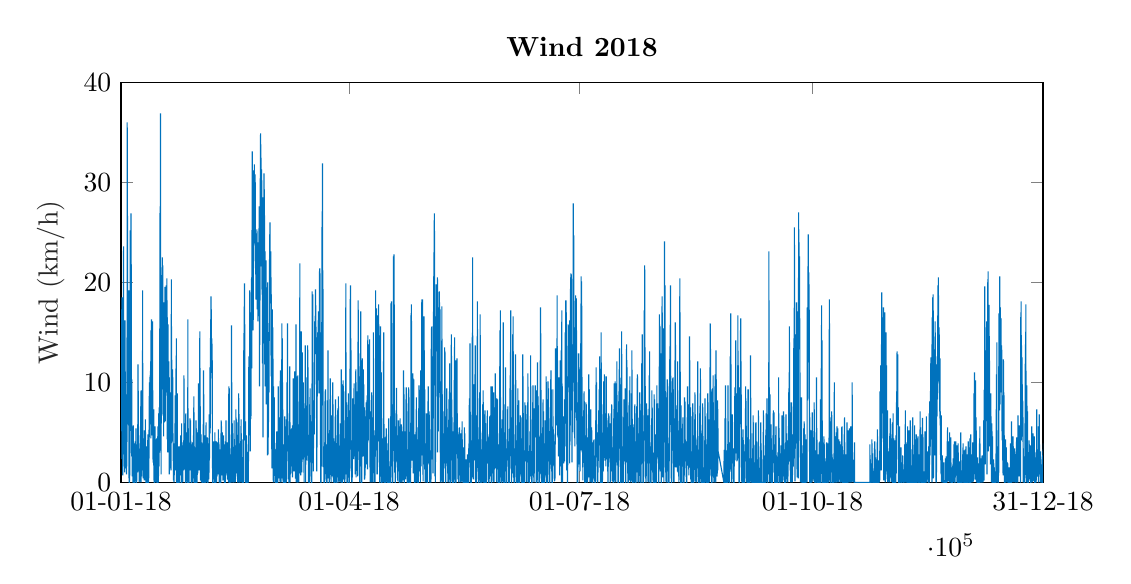
\begin{tikzpicture}

\begin{axis}[%
width=4.61in,
height=2in,
at={(0.758in,0.481in)},
scale only axis,
xmin=737061,
xmax=737425,
xtick={736969,737061,737151,737242,737334,737425},
xticklabels={{01-10-17},{01-01-18},{01-04-18},{01-07-18},{01-10-18},{31-12-18}},
ymin=0,
ymax=40,
ylabel style={font=\color{white!15!black}},
ylabel={Wind (km/h)},
axis background/.style={fill=white},
title style={font=\bfseries},
title={Wind 2018},
legend style={legend cell align=left, align=left, draw=white!15!black}
]
\addplot [color=mycolor1, forget plot]
  table[row sep=crcr]{%
737061	2.4\\
737061.034722222	2.4\\
737061.069444444	5.2\\
737061.104166667	12.7\\
737061.138888889	17.3\\
737061.173611111	8.7\\
737061.208333333	6.6\\
737061.243055556	13.7\\
737061.277777778	13.1\\
737061.3125	8.7\\
737061.347222222	12.4\\
737061.381944444	18.5\\
737061.416666667	7\\
737061.451388889	12\\
737061.486111111	18.4\\
737061.520833333	15.6\\
737061.555555556	12.4\\
737061.590277778	6.3\\
737061.625	4.7\\
737061.659722222	2.5\\
737061.694444444	0.7\\
737061.729166667	1.7\\
737061.763888889	3.1\\
737061.798611111	1.6\\
737061.833333333	5.7\\
737061.868055556	7.4\\
737061.902777778	3\\
737061.9375	16.9\\
737061.972222222	21.8\\
737062.006944444	23.6\\
737062.041666667	6.3\\
737062.076388889	16.2\\
737062.111111111	8.3\\
737062.145833333	8.7\\
737062.184027778	9.8\\
737062.21875	7.7\\
737062.253472222	8.1\\
737062.288194444	11.2\\
737062.322916667	9.4\\
737062.357638889	8.5\\
737062.392361111	2.9\\
737062.427083333	1\\
737062.461805556	8.5\\
737062.496527778	9.7\\
737062.53125	14.1\\
737062.565972222	16.2\\
737062.600694444	11.8\\
737062.635416667	13\\
737062.670138889	7.1\\
737062.704861111	6.7\\
737062.739583333	3.3\\
737062.774305556	3.4\\
737062.809027778	3.3\\
737062.84375	8.8\\
737062.878472222	1.4\\
737062.913194444	3.8\\
737062.947916667	5.2\\
737062.982638889	5.5\\
737063.017361111	2.2\\
737063.052083333	2.3\\
737063.086805556	1.5\\
737063.121527778	6.6\\
737063.15625	0.8\\
737063.190972222	3.4\\
737063.225694444	3\\
737063.260416667	2.9\\
737063.295138889	1.6\\
737063.329861111	2.8\\
737063.364583333	8.3\\
737063.399305556	22\\
737063.434027778	36\\
737063.46875	29.9\\
737063.503472222	29.1\\
737063.538194444	26.5\\
737063.572916667	22.6\\
737063.607638889	10.5\\
737063.642361111	9.5\\
737063.677083333	17.1\\
737063.711805556	8.8\\
737063.746527778	12.9\\
737063.78125	12.7\\
737063.815972222	6.9\\
737063.850694444	5.8\\
737063.885416667	12.7\\
737063.920138889	16\\
737063.954861111	14.5\\
737063.989583333	5.7\\
737064.027777778	11.4\\
737064.0625	19.2\\
737064.097222222	10.8\\
737064.131944444	2.5\\
737064.166666667	0.5\\
737064.201388889	0\\
737064.236111111	0\\
737064.270833333	0\\
737064.305555556	0\\
737064.34375	0.2\\
737064.378472222	0.9\\
737064.413194444	2.7\\
737064.447916667	0.7\\
737064.482638889	1.4\\
737064.517361111	2.1\\
737064.552083333	7.6\\
737064.586805556	21.7\\
737064.621527778	25.2\\
737064.65625	20.5\\
737064.690972222	18.9\\
737064.725694444	18.5\\
737064.760416667	18.1\\
737064.795138889	21\\
737064.829861111	21.7\\
737064.864583333	21.5\\
737064.899305556	21.7\\
737064.934027778	26.9\\
737064.96875	25.2\\
737065.003472222	22.2\\
737065.038194444	21.1\\
737065.072916667	12.8\\
737065.107638889	8.2\\
737065.142361111	7\\
737065.177083333	2.6\\
737065.211805556	9.7\\
737065.246527778	10.3\\
737065.28125	8.8\\
737065.315972222	4.7\\
737065.350694444	4\\
737065.385416667	0.6\\
737065.420138889	3.4\\
737065.454861111	5.6\\
737065.489583333	3\\
737065.524305556	4.2\\
737065.559027778	1.4\\
737065.59375	2.8\\
737065.628472222	1.9\\
737065.663194444	4.3\\
737065.697916667	0.1\\
737065.732638889	0\\
737065.767361111	1.1\\
737065.802083333	0\\
737065.836805556	3.1\\
737065.871527778	5.7\\
737065.90625	3\\
737065.940972222	3.1\\
737065.975694444	1.9\\
737066.013888889	1.2\\
737066.048611111	0\\
737066.083333333	0.5\\
737066.118055556	0\\
737066.152777778	0\\
737066.1875	0\\
737066.222222222	3.4\\
737066.256944444	3.9\\
737066.291666667	0\\
737066.326388889	0\\
737066.361111111	1\\
737066.395833333	2.4\\
737066.430555556	0\\
737066.465277778	0.5\\
737066.5	3.4\\
737066.534722222	3.7\\
737066.569444444	4.1\\
737066.604166667	3.8\\
737066.638888889	1.9\\
737066.673611111	0.5\\
737066.708333333	0.1\\
737066.743055556	3.3\\
737066.777777778	3.4\\
737066.8125	2.9\\
737066.847222222	4\\
737066.881944444	4.4\\
737066.916666667	5.4\\
737066.951388889	4.2\\
737066.986111111	2.1\\
737067.024305556	0.5\\
737067.059027778	0.3\\
737067.09375	0.9\\
737067.128472222	0\\
737067.163194444	0\\
737067.201388889	0.3\\
737067.236111111	2.1\\
737067.270833333	1.7\\
737067.305555556	2\\
737067.340277778	3.8\\
737067.375	1.3\\
737067.409722222	1.1\\
737067.444444444	1.3\\
737067.479166667	1.9\\
737067.513888889	1\\
737067.548611111	2.8\\
737067.583333333	1.2\\
737067.618055556	5.6\\
737067.652777778	6.7\\
737067.6875	4.5\\
737067.722222222	11.8\\
737067.756944444	9.3\\
737067.791666667	9.1\\
737067.826388889	6.4\\
737067.861111111	1.4\\
737067.895833333	5.6\\
737067.930555556	5.5\\
737067.965277778	2.4\\
737068	2.1\\
737068.034722222	2.2\\
737068.069444444	1.7\\
737068.104166667	1.8\\
737068.138888889	0\\
737068.173611111	2.5\\
737068.208333333	3.1\\
737068.243055556	0.1\\
737068.277777778	1.5\\
737068.3125	2.2\\
737068.347222222	2.6\\
737068.381944444	0.2\\
737068.416666667	0.1\\
737068.451388889	0.4\\
737068.486111111	1.8\\
737068.520833333	3.9\\
737068.555555556	3.2\\
737068.590277778	3.6\\
737068.625	2.3\\
737068.659722222	3.4\\
737068.694444444	4.7\\
737068.729166667	4.3\\
737068.763888889	7.6\\
737068.798611111	1.6\\
737068.833333333	9.1\\
737068.868055556	0\\
737068.902777778	6.3\\
737068.9375	9.2\\
737068.972222222	1.7\\
737069.010416667	3.5\\
737069.045138889	1.4\\
737069.079861111	1.1\\
737069.114583333	0.6\\
737069.149305556	3.2\\
737069.1875	3.6\\
737069.222222222	7.6\\
737069.256944444	8.3\\
737069.291666667	6.1\\
737069.326388889	3\\
737069.361111111	7.1\\
737069.395833333	5.8\\
737069.430555556	13.2\\
737069.465277778	4.1\\
737069.5	1.2\\
737069.534722222	19.2\\
737069.569444444	7.5\\
737069.604166667	4\\
737069.638888889	4.5\\
737069.673611111	3.6\\
737069.708333333	4.4\\
737069.743055556	2.8\\
737069.777777778	0.4\\
737069.8125	1.7\\
737069.847222222	2.5\\
737069.881944444	3.1\\
737069.916666667	1.3\\
737069.951388889	2.6\\
737069.986111111	3.8\\
737070.020833333	4.4\\
737070.055555556	3.9\\
737070.090277778	4.3\\
737070.125	4\\
737070.159722222	0.2\\
737070.197916667	4.6\\
737070.232638889	3.9\\
737070.267361111	5.2\\
737070.302083333	3.1\\
737070.336805556	2.1\\
737070.371527778	0.9\\
737070.40625	3.1\\
737070.440972222	1\\
737070.475694444	3.1\\
737070.510416667	4.5\\
737070.545138889	4.2\\
737070.579861111	4.9\\
737070.614583333	6.3\\
737070.649305556	2.4\\
737070.684027778	5\\
737070.71875	2.6\\
737070.753472222	1.3\\
737070.788194444	0\\
737070.822916667	0\\
737070.857638889	0\\
737070.892361111	0\\
737070.927083333	0\\
737070.961805556	0\\
737070.996527778	0\\
737071.03125	1.5\\
737071.065972222	0.2\\
737071.100694444	3.6\\
737071.135416667	2.3\\
737071.173611111	2\\
737071.208333333	1.3\\
737071.243055556	2.2\\
737071.277777778	0\\
737071.3125	0\\
737071.347222222	0\\
737071.381944444	0\\
737071.416666667	0\\
737071.451388889	2.3\\
737071.486111111	3.9\\
737071.520833333	2.2\\
737071.555555556	3.7\\
737071.590277778	4.8\\
737071.625	3.8\\
737071.659722222	2.1\\
737071.694444444	0\\
737071.729166667	0\\
737071.763888889	0\\
737071.798611111	0\\
737071.833333333	1.9\\
737071.868055556	2.4\\
737071.902777778	0\\
737071.9375	0.7\\
737071.972222222	0.6\\
737072.006944444	2.9\\
737072.041666667	2.4\\
737072.076388889	6.5\\
737072.111111111	3.1\\
737072.145833333	7.6\\
737072.184027778	9.7\\
737072.21875	9.2\\
737072.253472222	10\\
737072.288194444	7\\
737072.322916667	6.8\\
737072.357638889	7.7\\
737072.392361111	8.6\\
737072.427083333	7.5\\
737072.461805556	10.7\\
737072.496527778	5.8\\
737072.53125	8\\
737072.565972222	6.5\\
737072.600694444	9.3\\
737072.635416667	9.4\\
737072.670138889	12.1\\
737072.704861111	10.3\\
737072.739583333	7.2\\
737072.774305556	4.4\\
737072.809027778	10.5\\
737072.84375	15.2\\
737072.878472222	5.4\\
737072.913194444	5.9\\
737072.947916667	8\\
737072.982638889	9.3\\
737073.017361111	8.5\\
737073.052083333	16.3\\
737073.086805556	14.9\\
737073.121527778	9.1\\
737073.15625	5\\
737073.194444444	9.4\\
737073.229166667	5.4\\
737073.263888889	5.1\\
737073.298611111	5.7\\
737073.333333333	4.7\\
737073.368055556	8.1\\
737073.402777778	7.3\\
737073.4375	16.1\\
737073.472222222	13.7\\
737073.506944444	8.7\\
737073.541666667	6.3\\
737073.576388889	4.2\\
737073.611111111	4.8\\
737073.645833333	2.2\\
737073.680555556	2\\
737073.715277778	4.8\\
737073.75	4.8\\
737073.784722222	7.2\\
737073.819444444	6.9\\
737073.854166667	5.4\\
737073.888888889	3.2\\
737073.923611111	1.7\\
737073.958333333	7.3\\
737073.993055556	0.2\\
737074.027777778	0.6\\
737074.0625	0\\
737074.097222222	0\\
737074.131944444	0\\
737074.166666667	0\\
737074.204861111	0.4\\
737074.239583333	3.1\\
737074.274305556	0\\
737074.309027778	1.4\\
737074.34375	1.7\\
737074.378472222	4\\
737074.413194444	2.3\\
737074.447916667	5.6\\
737074.482638889	3.5\\
737074.517361111	4.3\\
737074.552083333	4.2\\
737074.586805556	2.8\\
737074.621527778	3.2\\
737074.65625	1.5\\
737074.690972222	1.6\\
737074.725694444	1.7\\
737074.760416667	2.9\\
737074.795138889	2.2\\
737074.829861111	0\\
737074.864583333	1.8\\
737074.899305556	2.2\\
737074.934027778	3.3\\
737074.96875	3.3\\
737075.003472222	3.8\\
737075.038194444	0.6\\
737075.072916667	4.4\\
737075.107638889	2.9\\
737075.142361111	3.7\\
737075.177083333	2\\
737075.211805556	4.3\\
737075.246527778	1.3\\
737075.28125	0.6\\
737075.315972222	0\\
737075.350694444	0\\
737075.385416667	2.3\\
737075.420138889	2.3\\
737075.454861111	0.8\\
737075.489583333	4.6\\
737075.524305556	0\\
737075.559027778	5.6\\
737075.59375	0.9\\
737075.628472222	3.3\\
737075.663194444	3.1\\
737075.697916667	2.6\\
737075.732638889	0\\
737075.767361111	0.1\\
737075.802083333	3\\
737075.836805556	6.9\\
737075.871527778	1.8\\
737075.90625	3.7\\
737075.940972222	5.5\\
737075.975694444	2.2\\
737076.013888889	1.6\\
737076.048611111	3.8\\
737076.083333333	7.5\\
737076.118055556	3.5\\
737076.152777778	4.5\\
737076.190972222	3.9\\
737076.225694444	3\\
737076.260416667	3.2\\
737076.295138889	10.3\\
737076.329861111	22.8\\
737076.364583333	25\\
737076.399305556	26.7\\
737076.434027778	27.6\\
737076.46875	19.8\\
737076.503472222	21.6\\
737076.538194444	30.7\\
737076.572916667	36.9\\
737076.607638889	26.6\\
737076.642361111	34.3\\
737076.677083333	12.4\\
737076.711805556	6.4\\
737076.746527778	4\\
737076.78125	7.5\\
737076.815972222	0.8\\
737076.850694444	14.7\\
737076.885416667	12.4\\
737076.920138889	5.9\\
737076.954861111	6.7\\
737076.989583333	7.9\\
737077.024305556	8\\
737077.059027778	12\\
737077.09375	11.3\\
737077.128472222	15\\
737077.163194444	16.2\\
737077.197916667	15.9\\
737077.232638889	12.2\\
737077.267361111	11.9\\
737077.302083333	22.5\\
737077.336805556	13.2\\
737077.371527778	18.5\\
737077.40625	18\\
737077.440972222	13.4\\
737077.475694444	19.6\\
737077.510416667	21.7\\
737077.545138889	18.7\\
737077.579861111	9.3\\
737077.614583333	16.3\\
737077.649305556	7.2\\
737077.684027778	6.7\\
737077.71875	12.1\\
737077.753472222	14.1\\
737077.788194444	8.3\\
737077.822916667	4.6\\
737077.857638889	15.7\\
737077.892361111	17.2\\
737077.927083333	10.3\\
737077.961805556	8.9\\
737078	18\\
737078.034722222	10.3\\
737078.069444444	10.4\\
737078.104166667	6\\
737078.138888889	13.2\\
737078.173611111	8.2\\
737078.208333333	12.3\\
737078.243055556	9.1\\
737078.277777778	6.1\\
737078.3125	10.9\\
737078.347222222	19.5\\
737078.381944444	19.5\\
737078.416666667	16.9\\
737078.451388889	13.2\\
737078.486111111	7.6\\
737078.520833333	6.1\\
737078.555555556	11.3\\
737078.590277778	16.6\\
737078.625	14.7\\
737078.659722222	12.9\\
737078.694444444	17.6\\
737078.729166667	14.7\\
737078.763888889	11.8\\
737078.798611111	15.3\\
737078.833333333	19.7\\
737078.868055556	17\\
737078.902777778	15.9\\
737078.9375	16.3\\
737078.972222222	9.1\\
737079.010416667	10.9\\
737079.045138889	13.8\\
737079.079861111	20.4\\
737079.114583333	9\\
737079.149305556	15.2\\
737079.1875	18.2\\
737079.222222222	4.3\\
737079.256944444	16.5\\
737079.291666667	5.6\\
737079.326388889	9\\
737079.361111111	6.5\\
737079.395833333	4.4\\
737079.430555556	5.8\\
737079.465277778	3\\
737079.5	14\\
737079.534722222	15.8\\
737079.569444444	8.7\\
737079.604166667	5.9\\
737079.638888889	3.3\\
737079.673611111	8.8\\
737079.708333333	5.1\\
737079.743055556	6.7\\
737079.777777778	3.8\\
737079.8125	9.9\\
737079.847222222	12.1\\
737079.881944444	8.2\\
737079.916666667	3.1\\
737079.951388889	8.4\\
737079.986111111	8.5\\
737080.020833333	0.8\\
737080.055555556	10.5\\
737080.090277778	3.4\\
737080.125	2.9\\
737080.159722222	3.8\\
737080.197916667	3.8\\
737080.232638889	8.1\\
737080.267361111	4.8\\
737080.302083333	1.4\\
737080.336805556	6.7\\
737080.371527778	9\\
737080.40625	8.3\\
737080.440972222	6.9\\
737080.475694444	3.8\\
737080.510416667	4.6\\
737080.545138889	3.5\\
737080.579861111	2.5\\
737080.614583333	3.5\\
737080.649305556	3.4\\
737080.684027778	4.8\\
737080.71875	1.2\\
737080.753472222	3.4\\
737080.788194444	2.4\\
737080.822916667	5.1\\
737080.857638889	20.3\\
737080.892361111	15.6\\
737080.927083333	12.2\\
737080.961805556	15.6\\
737080.996527778	4.1\\
737081.03125	12.2\\
737081.065972222	12.2\\
737081.100694444	12\\
737081.135416667	4.7\\
737081.170138889	9.8\\
737081.204861111	7.9\\
737081.239583333	9.8\\
737081.274305556	9.1\\
737081.309027778	11.3\\
737081.34375	7.2\\
737081.378472222	11\\
737081.413194444	9.7\\
737081.447916667	10.5\\
737081.482638889	4.5\\
737081.517361111	4.9\\
737081.552083333	3.6\\
737081.586805556	3\\
737081.621527778	2.7\\
737081.65625	1.7\\
737081.690972222	1.4\\
737081.725694444	0.2\\
737081.760416667	3.9\\
737081.795138889	0.8\\
737081.829861111	3.4\\
737081.864583333	3.2\\
737081.899305556	0\\
737081.934027778	0.7\\
737081.96875	0\\
737082.006944444	1.2\\
737082.041666667	1.6\\
737082.076388889	2.5\\
737082.111111111	1.5\\
737082.145833333	2.6\\
737082.180555556	2\\
737082.215277778	3.2\\
737082.25	3\\
737082.284722222	5.9\\
737082.319444444	3.7\\
737082.354166667	8.7\\
737082.388888889	6.7\\
737082.423611111	4.2\\
737082.458333333	5.4\\
737082.493055556	1.2\\
737082.527777778	3.1\\
737082.5625	1.2\\
737082.597222222	3.9\\
737082.631944444	1.6\\
737082.666666667	7.8\\
737082.701388889	9.4\\
737082.736111111	12.3\\
737082.770833333	6.1\\
737082.805555556	10.7\\
737082.840277778	14.4\\
737082.875	9.4\\
737082.909722222	0.1\\
737082.944444444	1.9\\
737082.979166667	0.5\\
737083.017361111	0\\
737083.052083333	0.2\\
737083.086805556	0\\
737083.121527778	0\\
737083.15625	4.4\\
737083.190972222	8.9\\
737083.225694444	0\\
737083.260416667	1.8\\
737083.295138889	0.8\\
737083.329861111	0\\
737083.364583333	0\\
737083.399305556	0.9\\
737083.434027778	0\\
737083.46875	0\\
737083.503472222	1.7\\
737083.538194444	2.9\\
737083.572916667	2\\
737083.607638889	3.6\\
737083.642361111	3.5\\
737083.677083333	0.5\\
737083.711805556	0.9\\
737083.746527778	0.1\\
737083.78125	0\\
737083.815972222	0\\
737083.850694444	0\\
737083.885416667	0\\
737083.920138889	3.6\\
737083.954861111	1.7\\
737083.989583333	0\\
737084.027777778	2.2\\
737084.0625	2.7\\
737084.097222222	3.4\\
737084.131944444	1.4\\
737084.166666667	2.5\\
737084.204861111	0.8\\
737084.239583333	2.1\\
737084.274305556	1.3\\
737084.309027778	2.1\\
737084.34375	0.7\\
737084.378472222	1.3\\
737084.413194444	2.1\\
737084.447916667	3.8\\
737084.482638889	1\\
737084.517361111	4.7\\
737084.552083333	4.1\\
737084.586805556	4.3\\
737084.621527778	2\\
737084.65625	3.9\\
737084.690972222	1.9\\
737084.725694444	0.9\\
737084.760416667	0.8\\
737084.795138889	0\\
737084.829861111	0\\
737084.864583333	3.9\\
737084.899305556	3\\
737084.934027778	5.9\\
737084.96875	1.4\\
737085.003472222	3.1\\
737085.038194444	2.4\\
737085.072916667	2.8\\
737085.107638889	3.4\\
737085.142361111	3\\
737085.180555556	3.4\\
737085.215277778	3.7\\
737085.25	2.1\\
737085.284722222	1.8\\
737085.319444444	2.7\\
737085.354166667	0.8\\
737085.388888889	0\\
737085.423611111	2.3\\
737085.458333333	2.4\\
737085.493055556	1.7\\
737085.527777778	4\\
737085.5625	3.7\\
737085.597222222	3\\
737085.631944444	1.2\\
737085.666666667	2.3\\
737085.701388889	1.2\\
737085.736111111	4.2\\
737085.770833333	2.1\\
737085.805555556	2.7\\
737085.840277778	10.7\\
737085.875	2.7\\
737085.909722222	1.5\\
737085.944444444	2.7\\
737085.979166667	1.3\\
737086.013888889	1.8\\
737086.048611111	4.9\\
737086.083333333	3.4\\
737086.118055556	2.9\\
737086.152777778	5.9\\
737086.190972222	3.2\\
737086.225694444	3.2\\
737086.260416667	3.2\\
737086.295138889	3.2\\
737086.329861111	3.2\\
737086.364583333	3.2\\
737086.399305556	0\\
737086.434027778	0\\
737086.46875	0\\
737086.506944444	5.7\\
737086.541666667	5.6\\
737086.576388889	6.9\\
737086.611111111	2.3\\
737086.645833333	2.5\\
737086.680555556	0.1\\
737086.715277778	0.7\\
737086.75	3.4\\
737086.784722222	4.6\\
737086.819444444	5\\
737086.854166667	3.6\\
737086.888888889	3.5\\
737086.923611111	2.7\\
737086.958333333	0.5\\
737086.993055556	4\\
737087.027777778	3.4\\
737087.0625	2.6\\
737087.097222222	1.6\\
737087.131944444	0\\
737087.166666667	0.3\\
737087.204861111	0\\
737087.239583333	0\\
737087.274305556	0\\
737087.309027778	0\\
737087.34375	0\\
737087.378472222	16.3\\
737087.413194444	5.5\\
737087.447916667	7.4\\
737087.482638889	6.4\\
737087.517361111	4.8\\
737087.552083333	5.4\\
737087.586805556	2.9\\
737087.621527778	3.8\\
737087.65625	1.8\\
737087.690972222	1.1\\
737087.725694444	0\\
737087.760416667	3.6\\
737087.795138889	0.7\\
737087.829861111	0\\
737087.864583333	0\\
737087.899305556	3\\
737087.934027778	2.5\\
737087.96875	3.6\\
737088.003472222	3.4\\
737088.038194444	2.4\\
737088.072916667	1.8\\
737088.107638889	1.9\\
737088.142361111	3.8\\
737088.180555556	4.4\\
737088.215277778	6.4\\
737088.25	4.4\\
737088.284722222	5.2\\
737088.319444444	3.1\\
737088.354166667	1.2\\
737088.388888889	3.5\\
737088.423611111	5.5\\
737088.458333333	6.2\\
737088.493055556	5.7\\
737088.527777778	1.5\\
737088.5625	1.3\\
737088.597222222	3.1\\
737088.631944444	1.5\\
737088.666666667	1.7\\
737088.701388889	2.8\\
737088.736111111	0\\
737088.770833333	0\\
737088.805555556	1.6\\
737088.840277778	2.6\\
737088.875	2\\
737088.909722222	0.7\\
737088.944444444	0.1\\
737088.979166667	2.2\\
737089.013888889	2.7\\
737089.048611111	3\\
737089.083333333	3.8\\
737089.118055556	0.1\\
737089.152777778	4\\
737089.190972222	1\\
737089.225694444	2.3\\
737089.260416667	0\\
737089.295138889	1.1\\
737089.329861111	0.9\\
737089.364583333	3\\
737089.399305556	0.4\\
737089.434027778	1.1\\
737089.46875	3.4\\
737089.503472222	3.4\\
737089.538194444	3.1\\
737089.572916667	3.7\\
737089.607638889	2.5\\
737089.642361111	5.4\\
737089.677083333	5.2\\
737089.711805556	5.8\\
737089.746527778	8.6\\
737089.78125	8.3\\
737089.815972222	2.6\\
737089.850694444	0.7\\
737089.885416667	0\\
737089.920138889	0\\
737089.954861111	3.6\\
737089.989583333	3.5\\
737090.024305556	2.4\\
737090.059027778	1\\
737090.09375	1.7\\
737090.128472222	0\\
737090.163194444	0\\
737090.197916667	0\\
737090.232638889	0\\
737090.267361111	2.6\\
737090.302083333	2.6\\
737090.336805556	0\\
737090.371527778	0\\
737090.40625	0\\
737090.440972222	0.7\\
737090.475694444	3.5\\
737090.510416667	3\\
737090.545138889	3.8\\
737090.579861111	3.4\\
737090.614583333	6.2\\
737090.649305556	4.7\\
737090.684027778	5.4\\
737090.71875	4\\
737090.753472222	1.5\\
737090.788194444	4\\
737090.822916667	0.6\\
737090.857638889	1.7\\
737090.892361111	0\\
737090.927083333	0\\
737090.961805556	0.1\\
737091	2.4\\
737091.034722222	0\\
737091.069444444	0.6\\
737091.104166667	2.3\\
737091.138888889	2.3\\
737091.173611111	3.3\\
737091.208333333	5\\
737091.243055556	4\\
737091.277777778	1.9\\
737091.3125	0.9\\
737091.347222222	3.9\\
737091.381944444	1.6\\
737091.416666667	2.2\\
737091.451388889	4.1\\
737091.486111111	5.2\\
737091.520833333	5.3\\
737091.555555556	7.7\\
737091.590277778	9.9\\
737091.625	4.7\\
737091.659722222	4.2\\
737091.694444444	3.9\\
737091.729166667	2.7\\
737091.763888889	6.5\\
737091.798611111	1.2\\
737091.833333333	2.7\\
737091.868055556	2.8\\
737091.902777778	5.7\\
737091.9375	3.3\\
737091.972222222	1.2\\
737092.010416667	4\\
737092.045138889	8.2\\
737092.079861111	13.3\\
737092.114583333	15.1\\
737092.149305556	11.8\\
737092.184027778	10.3\\
737092.21875	9.9\\
737092.253472222	7.3\\
737092.288194444	5.8\\
737092.322916667	7.6\\
737092.357638889	0.2\\
737092.392361111	3.8\\
737092.427083333	2.6\\
737092.461805556	0.8\\
737092.496527778	2.6\\
737092.53125	0.3\\
737092.565972222	0.9\\
737092.600694444	4.8\\
737092.635416667	0.9\\
737092.670138889	0.5\\
737092.704861111	0\\
737092.739583333	1.4\\
737092.774305556	0.8\\
737092.809027778	2.7\\
737092.84375	4\\
737092.878472222	2.7\\
737092.913194444	3.6\\
737092.947916667	3.9\\
737092.982638889	1.1\\
737093.020833333	0.8\\
737093.055555556	0.4\\
737093.090277778	0.3\\
737093.125	0\\
737093.159722222	0\\
737093.197916667	0\\
737093.232638889	0.3\\
737093.267361111	0\\
737093.302083333	0\\
737093.336805556	0\\
737093.371527778	2.2\\
737093.40625	0.5\\
737093.440972222	4.3\\
737093.475694444	5\\
737093.510416667	8.6\\
737093.545138889	7.7\\
737093.579861111	11.2\\
737093.614583333	5.1\\
737093.649305556	8.8\\
737093.684027778	4.1\\
737093.71875	2\\
737093.753472222	0\\
737093.788194444	0.1\\
737093.822916667	0.9\\
737093.857638889	0.9\\
737093.892361111	0\\
737093.927083333	2.4\\
737093.961805556	1.1\\
737093.996527778	0.8\\
737094.03125	0\\
737094.065972222	4.7\\
737094.100694444	0\\
737094.135416667	0\\
737094.173611111	0.5\\
737094.208333333	0\\
737094.243055556	0.9\\
737094.277777778	0.7\\
737094.3125	0\\
737094.347222222	0.3\\
737094.381944444	0.5\\
737094.416666667	0.3\\
737094.451388889	3.2\\
737094.486111111	3.2\\
737094.520833333	5.7\\
737094.555555556	3.9\\
737094.590277778	6\\
737094.625	4.1\\
737094.659722222	1.6\\
737094.694444444	4.2\\
737094.729166667	1.1\\
737094.763888889	0\\
737094.798611111	1.3\\
737094.833333333	3.5\\
737094.868055556	1.7\\
737094.902777778	0\\
737094.9375	2.1\\
737094.972222222	2.9\\
737095.006944444	3.7\\
737095.041666667	1.3\\
737095.076388889	4.5\\
737095.111111111	3.7\\
737095.145833333	1.6\\
737095.184027778	0\\
737095.21875	0\\
737095.253472222	3.8\\
737095.288194444	2.3\\
737095.322916667	2.7\\
737095.357638889	0.8\\
737095.392361111	0\\
737095.427083333	3.8\\
737095.461805556	1.6\\
737095.496527778	2.7\\
737095.53125	3.9\\
737095.565972222	2.1\\
737095.600694444	2.4\\
737095.635416667	1.5\\
737095.670138889	3.1\\
737095.704861111	0.3\\
737095.739583333	4\\
737095.774305556	5.1\\
737095.809027778	6.8\\
737095.84375	5.3\\
737095.878472222	2.2\\
737095.913194444	6\\
737095.947916667	2.9\\
737095.982638889	2.4\\
737096.017361111	6.6\\
737096.052083333	6.5\\
737096.086805556	6.6\\
737096.121527778	11.5\\
737096.15625	7.4\\
737096.190972222	4.9\\
737096.225694444	6.3\\
737096.260416667	8.9\\
737096.295138889	11.4\\
737096.329861111	14.4\\
737096.364583333	14.5\\
737096.399305556	16.3\\
737096.434027778	12.5\\
737096.46875	13.9\\
737096.503472222	18.6\\
737096.538194444	17.3\\
737096.572916667	17.1\\
737096.607638889	17\\
737096.642361111	17.3\\
737096.677083333	16.7\\
737096.711805556	11.7\\
737096.746527778	11.8\\
737096.78125	11.3\\
737096.815972222	12.1\\
737096.850694444	10.4\\
737096.885416667	14.4\\
737096.920138889	12.5\\
737096.954861111	11.5\\
737096.989583333	12.9\\
737097.027777778	7.4\\
737097.0625	5.1\\
737097.097222222	1.4\\
737097.131944444	3.7\\
737097.166666667	4.1\\
737097.204861111	0\\
737097.239583333	0\\
737097.274305556	0\\
737097.309027778	0.7\\
737097.34375	3.5\\
737097.378472222	3.5\\
737097.413194444	0.8\\
737097.447916667	1.6\\
737097.482638889	1.2\\
737097.517361111	2.5\\
737097.552083333	4.1\\
737097.586805556	1.7\\
737097.621527778	2.3\\
737097.65625	4.1\\
737097.690972222	2.9\\
737097.725694444	2.7\\
737097.760416667	0.9\\
737097.795138889	0.7\\
737097.829861111	2.8\\
737097.864583333	0\\
737097.899305556	0\\
737097.934027778	0\\
737097.96875	0\\
737098.003472222	0.3\\
737098.038194444	2.6\\
737098.072916667	5\\
737098.107638889	0.8\\
737098.142361111	1.9\\
737098.180555556	0\\
737098.215277778	0.2\\
737098.25	2.2\\
737098.284722222	0\\
737098.319444444	0\\
737098.354166667	0\\
737098.388888889	1.4\\
737098.423611111	3.6\\
737098.458333333	2.7\\
737098.493055556	3.9\\
737098.527777778	2.3\\
737098.5625	3.5\\
737098.597222222	3.8\\
737098.631944444	4.1\\
737098.666666667	1.7\\
737098.701388889	3\\
737098.736111111	0\\
737098.770833333	1\\
737098.805555556	2.3\\
737098.840277778	4\\
737098.875	0.6\\
737098.909722222	2\\
737098.944444444	2.5\\
737098.979166667	2.5\\
737099.013888889	4\\
737099.048611111	2.7\\
737099.083333333	1.6\\
737099.118055556	3.4\\
737099.152777778	2.4\\
737099.190972222	2\\
737099.225694444	0.8\\
737099.260416667	3.2\\
737099.295138889	1.8\\
737099.329861111	2.6\\
737099.364583333	2.7\\
737099.399305556	3.1\\
737099.434027778	5.3\\
737099.46875	4.2\\
737099.503472222	3.3\\
737099.538194444	2.9\\
737099.572916667	4\\
737099.607638889	3.1\\
737099.642361111	3.6\\
737099.677083333	3.8\\
737099.711805556	2.2\\
737099.746527778	1.6\\
737099.78125	0\\
737099.815972222	2.6\\
737099.850694444	0\\
737099.885416667	0\\
737099.920138889	2.8\\
737099.954861111	0.1\\
737099.989583333	3\\
737100.024305556	3.3\\
737100.059027778	1.7\\
737100.09375	0.8\\
737100.128472222	1.7\\
737100.163194444	0\\
737100.197916667	0.6\\
737100.232638889	0\\
737100.267361111	0\\
737100.302083333	0\\
737100.336805556	0.2\\
737100.371527778	0\\
737100.40625	0\\
737100.440972222	0.3\\
737100.475694444	4.9\\
737100.510416667	4.7\\
737100.545138889	6.2\\
737100.579861111	4.7\\
737100.614583333	3\\
737100.649305556	4.7\\
737100.684027778	5.6\\
737100.71875	0.7\\
737100.753472222	2\\
737100.788194444	1.7\\
737100.822916667	1.9\\
737100.857638889	4.1\\
737100.892361111	3.3\\
737100.927083333	0.8\\
737100.961805556	1.6\\
737101	5\\
737101.034722222	2.2\\
737101.069444444	3.2\\
737101.104166667	3\\
737101.138888889	2.5\\
737101.177083333	1.9\\
737101.211805556	0.7\\
737101.246527778	0.2\\
737101.28125	1.5\\
737101.315972222	1.1\\
737101.350694444	3.2\\
737101.385416667	1.3\\
737101.420138889	4.3\\
737101.454861111	4.7\\
737101.489583333	2.3\\
737101.524305556	2.4\\
737101.559027778	2.3\\
737101.59375	3.5\\
737101.628472222	1.4\\
737101.663194444	3.8\\
737101.697916667	1.6\\
737101.732638889	1.4\\
737101.767361111	1.4\\
737101.802083333	0\\
737101.836805556	0\\
737101.871527778	0\\
737101.90625	0\\
737101.940972222	1.3\\
737101.975694444	0\\
737102.010416667	0\\
737102.045138889	0\\
737102.079861111	0\\
737102.114583333	0\\
737102.149305556	0\\
737102.184027778	1.5\\
737102.21875	0.5\\
737102.253472222	4.1\\
737102.288194444	1.4\\
737102.322916667	3.7\\
737102.357638889	0.9\\
737102.392361111	3.1\\
737102.427083333	6.2\\
737102.461805556	5.6\\
737102.496527778	5.2\\
737102.53125	1.8\\
737102.565972222	2.6\\
737102.600694444	3.7\\
737102.635416667	1.8\\
737102.670138889	1.6\\
737102.704861111	1.3\\
737102.739583333	1.4\\
737102.774305556	0.7\\
737102.809027778	2.1\\
737102.84375	0.8\\
737102.878472222	4\\
737102.913194444	2.2\\
737102.947916667	0.9\\
737102.982638889	2.7\\
737103.020833333	0.3\\
737103.055555556	0.5\\
737103.090277778	1.2\\
737103.125	2.8\\
737103.159722222	0.8\\
737103.197916667	3.2\\
737103.232638889	1.6\\
737103.267361111	2.2\\
737103.302083333	1.6\\
737103.336805556	2.8\\
737103.371527778	0\\
737103.40625	5.1\\
737103.440972222	5\\
737103.475694444	8.8\\
737103.510416667	8.8\\
737103.545138889	2.8\\
737103.579861111	9.6\\
737103.614583333	7.5\\
737103.649305556	5.6\\
737103.684027778	7.3\\
737103.71875	9.4\\
737103.753472222	4.4\\
737103.788194444	5.1\\
737103.822916667	0\\
737103.857638889	0\\
737103.892361111	3.4\\
737103.927083333	0.7\\
737103.961805556	0\\
737103.996527778	0\\
737104.03125	0.6\\
737104.065972222	0\\
737104.100694444	1.6\\
737104.135416667	1.2\\
737104.170138889	0\\
737104.204861111	1.3\\
737104.239583333	0\\
737104.274305556	0.2\\
737104.309027778	0\\
737104.34375	0.2\\
737104.378472222	0\\
737104.413194444	2.8\\
737104.447916667	2.3\\
737104.482638889	3.7\\
737104.517361111	4.6\\
737104.552083333	4.9\\
737104.586805556	13.5\\
737104.621527778	15.7\\
737104.65625	11.1\\
737104.690972222	8.8\\
737104.725694444	10\\
737104.760416667	7.9\\
737104.795138889	3\\
737104.829861111	0\\
737104.864583333	4\\
737104.899305556	3.6\\
737104.934027778	5.9\\
737104.96875	2.4\\
737105.006944444	0\\
737105.041666667	1\\
737105.076388889	1.2\\
737105.111111111	1.7\\
737105.145833333	3.1\\
737105.180555556	3.4\\
737105.215277778	2.7\\
737105.25	1.5\\
737105.284722222	3.5\\
737105.319444444	2.6\\
737105.354166667	0\\
737105.388888889	0.4\\
737105.423611111	0\\
737105.458333333	2.4\\
737105.493055556	1.7\\
737105.527777778	3.8\\
737105.5625	4.8\\
737105.597222222	4.9\\
737105.631944444	3.2\\
737105.666666667	6.2\\
737105.701388889	1.2\\
737105.736111111	0\\
737105.770833333	2.6\\
737105.805555556	2.7\\
737105.840277778	2.5\\
737105.875	1.9\\
737105.909722222	2.4\\
737105.944444444	0\\
737105.979166667	1.7\\
737106.017361111	3.7\\
737106.052083333	2.2\\
737106.086805556	1\\
737106.121527778	1.2\\
737106.15625	0\\
737106.190972222	0.7\\
737106.225694444	2.2\\
737106.260416667	2.2\\
737106.295138889	0.8\\
737106.329861111	0.6\\
737106.364583333	7.3\\
737106.399305556	2.5\\
737106.434027778	1.6\\
737106.46875	5.9\\
737106.503472222	1.2\\
737106.538194444	4.8\\
737106.572916667	1.6\\
737106.607638889	3.4\\
737106.642361111	6.3\\
737106.677083333	4.1\\
737106.711805556	2.1\\
737106.746527778	0.9\\
737106.78125	2.8\\
737106.815972222	3.7\\
737106.850694444	3.2\\
737106.885416667	1.9\\
737106.920138889	2.9\\
737106.954861111	1.6\\
737106.989583333	2.5\\
737107.027777778	3\\
737107.0625	0.2\\
737107.097222222	0\\
737107.131944444	1.4\\
737107.166666667	3.5\\
737107.204861111	1\\
737107.239583333	2.9\\
737107.274305556	6\\
737107.309027778	4.9\\
737107.34375	6\\
737107.378472222	4.7\\
737107.413194444	4.9\\
737107.447916667	8.9\\
737107.482638889	6.9\\
737107.517361111	7.1\\
737107.552083333	7.1\\
737107.586805556	4.3\\
737107.621527778	1.7\\
737107.65625	0\\
737107.690972222	2.9\\
737107.725694444	0.3\\
737107.760416667	0\\
737107.795138889	3.3\\
737107.829861111	0.9\\
737107.864583333	0.6\\
737107.899305556	1.4\\
737107.934027778	2.7\\
737107.96875	3.4\\
737108.003472222	2.9\\
737108.038194444	0\\
737108.072916667	0.5\\
737108.107638889	0\\
737108.142361111	2.7\\
737108.177083333	3.9\\
737108.211805556	1.2\\
737108.246527778	2.9\\
737108.28125	3.8\\
737108.315972222	5.5\\
737108.350694444	3.8\\
737108.385416667	5.6\\
737108.420138889	6.3\\
737108.454861111	4.2\\
737108.489583333	2.5\\
737108.524305556	4.4\\
737108.559027778	3.8\\
737108.59375	3.5\\
737108.628472222	0\\
737108.663194444	3.8\\
737108.697916667	3.5\\
737108.732638889	3.8\\
737108.767361111	4.3\\
737108.802083333	2.9\\
737108.836805556	2.6\\
737108.871527778	1.4\\
737108.90625	0\\
737108.940972222	0\\
737108.975694444	0\\
737109.013888889	0\\
737109.048611111	0\\
737109.083333333	0\\
737109.118055556	0\\
737109.152777778	0\\
737109.1875	0\\
737109.222222222	0\\
737109.256944444	0\\
737109.291666667	0\\
737109.326388889	0\\
737109.361111111	0\\
737109.395833333	0\\
737109.430555556	12.4\\
737109.465277778	13.2\\
737109.5	11.5\\
737109.534722222	13.5\\
737109.569444444	14.9\\
737109.604166667	15.6\\
737109.638888889	16.8\\
737109.673611111	17.7\\
737109.708333333	15\\
737109.743055556	19.9\\
737109.777777778	17.8\\
737109.8125	16\\
737109.847222222	15.5\\
737109.881944444	7.7\\
737109.916666667	6.2\\
737109.951388889	4.2\\
737109.986111111	5.2\\
737110.024305556	5.2\\
737110.059027778	5.9\\
737110.09375	5\\
737110.128472222	6.1\\
737110.163194444	0\\
737110.201388889	0.3\\
737110.236111111	0.6\\
737110.270833333	0\\
737110.305555556	0\\
737110.340277778	0\\
737110.375	0\\
737110.409722222	2.1\\
737110.444444444	1.4\\
737110.479166667	2.4\\
737110.513888889	4.7\\
737110.548611111	3.6\\
737110.583333333	1.5\\
737110.618055556	0.9\\
737110.652777778	1.8\\
737110.6875	3\\
737110.722222222	3\\
737110.756944444	1.5\\
737110.791666667	1.2\\
737110.826388889	0\\
737110.861111111	0\\
737110.895833333	0\\
737110.930555556	0.8\\
737110.965277778	0\\
737111	0\\
737111.034722222	0\\
737111.069444444	1.8\\
737111.104166667	0.3\\
737111.138888889	0.2\\
737111.173611111	0\\
737111.208333333	1.6\\
737111.243055556	0\\
737111.277777778	3.3\\
737111.3125	3.8\\
737111.347222222	2.1\\
737111.381944444	4\\
737111.416666667	5.8\\
737111.451388889	12.6\\
737111.486111111	10.8\\
737111.520833333	11\\
737111.555555556	10.9\\
737111.590277778	7.7\\
737111.625	4.7\\
737111.659722222	10.1\\
737111.694444444	10.4\\
737111.729166667	10.3\\
737111.763888889	15.2\\
737111.798611111	19.2\\
737111.833333333	10.9\\
737111.868055556	10\\
737111.902777778	10.2\\
737111.9375	9.2\\
737111.972222222	10.8\\
737112.010416667	3.1\\
737112.045138889	4.5\\
737112.079861111	8.9\\
737112.114583333	13.6\\
737112.149305556	14.5\\
737112.1875	6.4\\
737112.222222222	6.4\\
737112.256944444	6.4\\
737112.291666667	6.4\\
737112.326388889	12.9\\
737112.361111111	15.7\\
737112.395833333	16.6\\
737112.430555556	17\\
737112.465277778	13.2\\
737112.5	18.9\\
737112.534722222	20.5\\
737112.569444444	18.1\\
737112.604166667	11.4\\
737112.638888889	19.8\\
737112.673611111	18.5\\
737112.708333333	22.7\\
737112.743055556	26.9\\
737112.777777778	33\\
737112.8125	33.1\\
737112.847222222	23.3\\
737112.881944444	25.8\\
737112.916666667	29.9\\
737112.951388889	27\\
737112.986111111	25.7\\
737113.020833333	27.8\\
737113.055555556	20.7\\
737113.090277778	23.3\\
737113.125	16.4\\
737113.159722222	15.2\\
737113.197916667	17.1\\
737113.232638889	22.4\\
737113.267361111	21.6\\
737113.302083333	23.2\\
737113.336805556	31.2\\
737113.371527778	30.8\\
737113.40625	30.7\\
737113.440972222	28.2\\
737113.475694444	23.7\\
737113.510416667	28.6\\
737113.545138889	27.1\\
737113.579861111	29.3\\
737113.614583333	31\\
737113.649305556	31.8\\
737113.684027778	27.6\\
737113.71875	25.2\\
737113.753472222	25.3\\
737113.788194444	23.9\\
737113.822916667	24.5\\
737113.857638889	30.6\\
737113.892361111	28.4\\
737113.927083333	27.9\\
737113.961805556	30.8\\
737113.996527778	24\\
737114.03125	30\\
737114.065972222	21.4\\
737114.100694444	24\\
737114.135416667	24.5\\
737114.174305556	23.6\\
737114.208333333	20.8\\
737114.243055556	24.3\\
737114.277777778	18.3\\
737114.3125	18.5\\
737114.347222222	19.2\\
737114.381944444	20.1\\
737114.416666667	20.1\\
737114.451388889	21.9\\
737114.486111111	23.6\\
737114.520833333	24.9\\
737114.555555556	24.2\\
737114.590277778	22.4\\
737114.625	25.3\\
737114.659722222	20.9\\
737114.694444444	25.1\\
737114.729166667	24.7\\
737114.763888889	23.2\\
737114.798611111	17.3\\
737114.833333333	20.6\\
737114.868055556	19.9\\
737114.902777778	22.7\\
737114.9375	24\\
737114.972222222	20\\
737115.006944444	20.7\\
737115.041666667	16.1\\
737115.076388889	17.4\\
737115.111111111	17.6\\
737115.145833333	18.4\\
737115.180555556	18.6\\
737115.215277778	18.3\\
737115.25	18.6\\
737115.284722222	23.6\\
737115.319444444	21.3\\
737115.354166667	23.6\\
737115.388888889	22.7\\
737115.423611111	24.9\\
737115.458333333	25.4\\
737115.493055556	22.6\\
737115.527777778	24.4\\
737115.5625	27.6\\
737115.597222222	22.6\\
737115.631944444	22.2\\
737115.666666667	9.6\\
737115.701388889	13.9\\
737115.736111111	13.2\\
737115.770833333	15.1\\
737115.805555556	17.4\\
737115.840277778	20.7\\
737115.875	18.2\\
737115.909722222	28.9\\
737115.944444444	28.4\\
737115.979166667	30.4\\
737116.017361111	27.5\\
737116.052083333	32.6\\
737116.086805556	34.9\\
737116.121527778	32.7\\
737116.15625	32.8\\
737116.194444444	30.4\\
737116.229166667	33.8\\
737116.263888889	29.5\\
737116.298611111	23.7\\
737116.333333333	23.3\\
737116.368055556	24.5\\
737116.402777778	21.6\\
737116.4375	24\\
737116.472222222	22.4\\
737116.506944444	31.3\\
737116.541666667	30\\
737116.576388889	24.7\\
737116.611111111	19.3\\
737116.645833333	23.2\\
737116.680555556	19.5\\
737116.715277778	18.8\\
737116.75	19.7\\
737116.784722222	18.5\\
737116.819444444	11.9\\
737116.854166667	12.8\\
737116.888888889	12.1\\
737116.923611111	15.6\\
737116.958333333	16.8\\
737116.993055556	22.2\\
737117.027777778	20.5\\
737117.0625	4.5\\
737117.097222222	21.6\\
737117.131944444	28.5\\
737117.166666667	26.4\\
737117.204861111	27.1\\
737117.239583333	27\\
737117.274305556	19.5\\
737117.309027778	22.6\\
737117.34375	19.7\\
737117.378472222	13.9\\
737117.413194444	21.8\\
737117.447916667	30.9\\
737117.482638889	22.7\\
737117.517361111	24\\
737117.552083333	26.6\\
737117.586805556	29.3\\
737117.621527778	26.8\\
737117.65625	24.4\\
737117.690972222	22\\
737117.725694444	21.4\\
737117.760416667	11.8\\
737117.795138889	17.9\\
737117.829861111	23.1\\
737117.864583333	21.2\\
737117.899305556	11.4\\
737117.934027778	9.6\\
737117.96875	15.5\\
737118.003472222	9.9\\
737118.038194444	11.7\\
737118.072916667	11.8\\
737118.107638889	15.5\\
737118.142361111	11.9\\
737118.180555556	18.7\\
737118.215277778	17.5\\
737118.25	22.2\\
737118.284722222	7.8\\
737118.319444444	9.2\\
737118.354166667	15.8\\
737118.388888889	16.7\\
737118.423611111	14.9\\
737118.458333333	16.5\\
737118.493055556	13.2\\
737118.527777778	18.6\\
737118.5625	11.5\\
737118.597222222	19.2\\
737118.631944444	17.9\\
737118.666666667	19.5\\
737118.701388889	14.6\\
737118.736111111	12.4\\
737118.770833333	18\\
737118.805555556	16.6\\
737118.840277778	2.7\\
737118.875	20\\
737118.909722222	14.2\\
737118.944444444	3.7\\
737118.979166667	8.2\\
737119.013888889	2.8\\
737119.048611111	7.7\\
737119.083333333	9\\
737119.118055556	5.7\\
737119.152777778	11.2\\
737119.1875	4.5\\
737119.222222222	8.4\\
737119.256944444	8.2\\
737119.291666667	11.7\\
737119.326388889	9.1\\
737119.361111111	12.8\\
737119.395833333	12.5\\
737119.430555556	9\\
737119.465277778	11\\
737119.5	14.5\\
737119.534722222	15.8\\
737119.569444444	16.7\\
737119.604166667	20.4\\
737119.638888889	22.4\\
737119.673611111	24.8\\
737119.708333333	17.9\\
737119.743055556	25.9\\
737119.777777778	22.1\\
737119.8125	26\\
737119.847222222	24.7\\
737119.881944444	20.6\\
737119.916666667	21.7\\
737119.951388889	18.3\\
737119.986111111	18.9\\
737120.024305556	20\\
737120.059027778	20.9\\
737120.09375	23.1\\
737120.128472222	19.4\\
737120.163194444	12.7\\
737120.197916667	20.5\\
737120.232638889	15\\
737120.267361111	10.6\\
737120.302083333	16.5\\
737120.336805556	18.8\\
737120.371527778	14.7\\
737120.40625	16.3\\
737120.440972222	14.9\\
737120.475694444	8.2\\
737120.510416667	5\\
737120.545138889	1.4\\
737120.579861111	5.3\\
737120.614583333	5.3\\
737120.649305556	5.9\\
737120.684027778	13.1\\
737120.71875	17.3\\
737120.753472222	16.9\\
737120.788194444	14.4\\
737120.822916667	13.2\\
737120.857638889	14.2\\
737120.892361111	10.6\\
737120.927083333	15.5\\
737120.961805556	14.4\\
737121	9.3\\
737121.034722222	6.2\\
737121.069444444	5.4\\
737121.104166667	0.2\\
737121.138888889	3.7\\
737121.173611111	0\\
737121.208333333	5.7\\
737121.243055556	9.6\\
737121.277777778	1.9\\
737121.3125	1.4\\
737121.347222222	0\\
737121.381944444	4.8\\
737121.416666667	4.8\\
737121.451388889	5.5\\
737121.486111111	8.5\\
737121.520833333	3.6\\
737121.555555556	2.7\\
737121.590277778	1.6\\
737121.625	1.2\\
737121.659722222	3.9\\
737121.694444444	3.9\\
737121.729166667	2.7\\
737121.763888889	3.4\\
737121.798611111	3.1\\
737121.833333333	2.7\\
737121.868055556	1.5\\
737121.902777778	0.8\\
737121.9375	0\\
737121.972222222	3.1\\
737122.010416667	0\\
737122.045138889	0\\
737122.079861111	1.1\\
737122.114583333	2.1\\
737122.149305556	0\\
737122.1875	0.3\\
737122.222222222	0\\
737122.256944444	0\\
737122.291666667	0.3\\
737122.326388889	3.3\\
737122.361111111	1.2\\
737122.395833333	2.5\\
737122.430555556	1.6\\
737122.465277778	3\\
737122.5	5.1\\
737122.534722222	4\\
737122.569444444	1.9\\
737122.604166667	1.4\\
737122.638888889	2.3\\
737122.673611111	0\\
737122.708333333	1\\
737122.743055556	0\\
737122.777777778	0\\
737122.8125	2.5\\
737122.847222222	1.7\\
737122.881944444	0\\
737122.916666667	0.8\\
737122.951388889	1.9\\
737122.986111111	2.7\\
737123.020833333	0.6\\
737123.055555556	9.6\\
737123.090277778	6.8\\
737123.125	3.4\\
737123.159722222	3.3\\
737123.194444444	1.5\\
737123.229166667	2.5\\
737123.263888889	0.6\\
737123.298611111	0.9\\
737123.333333333	2.3\\
737123.368055556	2.6\\
737123.402777778	1.6\\
737123.4375	3.7\\
737123.472222222	0.4\\
737123.506944444	5.2\\
737123.541666667	6.5\\
737123.576388889	1.1\\
737123.611111111	6.4\\
737123.645833333	5.7\\
737123.680555556	3.4\\
737123.715277778	4.9\\
737123.75	2.7\\
737123.784722222	0\\
737123.819444444	3.2\\
737123.854166667	5.9\\
737123.888888889	11.2\\
737123.923611111	2.6\\
737123.958333333	2.5\\
737123.993055556	3.9\\
737124.03125	0.7\\
737124.065972222	3.7\\
737124.100694444	1.7\\
737124.135416667	2.6\\
737124.170138889	0\\
737124.204861111	2.3\\
737124.239583333	3.6\\
737124.274305556	3.9\\
737124.309027778	3.1\\
737124.34375	1.9\\
737124.378472222	0.4\\
737124.413194444	2\\
737124.447916667	0.8\\
737124.482638889	15.9\\
737124.517361111	14.1\\
737124.552083333	12.9\\
737124.586805556	13.5\\
737124.621527778	10.8\\
737124.65625	8.6\\
737124.690972222	14.4\\
737124.725694444	9.2\\
737124.760416667	5.5\\
737124.795138889	10\\
737124.829861111	7.1\\
737124.864583333	5.4\\
737124.899305556	4.5\\
737124.934027778	2.6\\
737124.96875	0.1\\
737125.006944444	1.8\\
737125.041666667	0\\
737125.076388889	0\\
737125.111111111	0\\
737125.145833333	2.7\\
737125.180555556	0\\
737125.215277778	2.3\\
737125.25	2.3\\
737125.284722222	0\\
737125.319444444	0\\
737125.354166667	0\\
737125.388888889	0\\
737125.423611111	3.1\\
737125.458333333	3.8\\
737125.493055556	2.3\\
737125.527777778	1.1\\
737125.5625	3.9\\
737125.597222222	6.6\\
737125.631944444	5.8\\
737125.666666667	6.6\\
737125.701388889	5.8\\
737125.736111111	5.3\\
737125.770833333	3\\
737125.805555556	0\\
737125.840277778	0\\
737125.875	2\\
737125.909722222	4.3\\
737125.944444444	0.8\\
737125.979166667	0.2\\
737126.017361111	0\\
737126.052083333	1\\
737126.086805556	0\\
737126.121527778	0.8\\
737126.15625	0.3\\
737126.194444444	1.4\\
737126.229166667	0\\
737126.263888889	2.9\\
737126.298611111	6.3\\
737126.333333333	3.6\\
737126.368055556	6\\
737126.402777778	3.6\\
737126.4375	4\\
737126.472222222	10\\
737126.506944444	5.3\\
737126.541666667	6.2\\
737126.576388889	8\\
737126.611111111	5.5\\
737126.645833333	7.2\\
737126.680555556	12.6\\
737126.715277778	15.9\\
737126.75	8.5\\
737126.784722222	4\\
737126.819444444	3.1\\
737126.854166667	3.5\\
737126.888888889	2.9\\
737126.923611111	4.2\\
737126.958333333	0.3\\
737126.993055556	3\\
737127.027777778	4.7\\
737127.0625	1.3\\
737127.097222222	3.1\\
737127.131944444	2.6\\
737127.166666667	4.3\\
737127.204861111	1.3\\
737127.239583333	1.9\\
737127.274305556	0\\
737127.309027778	0\\
737127.34375	2.1\\
737127.378472222	6.1\\
737127.413194444	2.5\\
737127.447916667	4.2\\
737127.482638889	6.9\\
737127.517361111	3.9\\
737127.552083333	5.3\\
737127.586805556	7.3\\
737127.621527778	11.6\\
737127.65625	7.6\\
737127.690972222	5.9\\
737127.725694444	2.4\\
737127.760416667	0\\
737127.795138889	2.5\\
737127.829861111	0.8\\
737127.864583333	2.2\\
737127.899305556	2.2\\
737127.934027778	2.9\\
737127.96875	0.9\\
737128.003472222	5.3\\
737128.038194444	0.9\\
737128.072916667	2.6\\
737128.107638889	4.5\\
737128.142361111	3.3\\
737128.177083333	3.5\\
737128.211805556	4.6\\
737128.246527778	2.2\\
737128.28125	1.6\\
737128.315972222	2.4\\
737128.350694444	4.8\\
737128.385416667	5.4\\
737128.420138889	3.9\\
737128.454861111	3.4\\
737128.489583333	3.6\\
737128.524305556	4.1\\
737128.559027778	2.7\\
737128.59375	3.4\\
737128.628472222	4.7\\
737128.663194444	5.7\\
737128.697916667	0.5\\
737128.732638889	3.1\\
737128.767361111	3.8\\
737128.802083333	4\\
737128.836805556	1.6\\
737128.871527778	1.7\\
737128.90625	2.1\\
737128.940972222	2.7\\
737128.975694444	10.4\\
737129.013888889	5.8\\
737129.048611111	1.6\\
737129.083333333	6.2\\
737129.118055556	1.9\\
737129.152777778	4.1\\
737129.1875	7.7\\
737129.222222222	6.6\\
737129.256944444	2\\
737129.291666667	1.1\\
737129.326388889	5.9\\
737129.361111111	3.5\\
737129.395833333	3.9\\
737129.430555556	6\\
737129.465277778	8.1\\
737129.5	2.4\\
737129.534722222	2.8\\
737129.569444444	11.1\\
737129.604166667	5.8\\
737129.638888889	6.2\\
737129.673611111	2.3\\
737129.708333333	2.7\\
737129.743055556	2.2\\
737129.777777778	1.9\\
737129.8125	0.9\\
737129.847222222	0.4\\
737129.881944444	0.5\\
737129.916666667	6.3\\
737129.951388889	2\\
737129.986111111	8.7\\
737130.024305556	3.5\\
737130.059027778	15.8\\
737130.09375	8.1\\
737130.128472222	3\\
737130.163194444	0\\
737130.201388889	1.8\\
737130.236111111	4.8\\
737130.270833333	1.1\\
737130.305555556	5\\
737130.340277778	4.8\\
737130.375	5\\
737130.409722222	10.6\\
737130.444444444	6.6\\
737130.479166667	1.1\\
737130.513888889	1.2\\
737130.548611111	5\\
737130.583333333	2.5\\
737130.618055556	0.4\\
737130.652777778	4.8\\
737130.6875	0.4\\
737130.722222222	0\\
737130.756944444	0.8\\
737130.791666667	3.9\\
737130.826388889	10.7\\
737130.861111111	6.5\\
737130.895833333	2.8\\
737130.930555556	0.5\\
737130.965277778	0\\
737131	1.1\\
737131.034722222	0\\
737131.069444444	2.9\\
737131.104166667	0\\
737131.138888889	3.4\\
737131.173611111	0.7\\
737131.208333333	0\\
737131.243055556	2.5\\
737131.277777778	3\\
737131.3125	1.6\\
737131.347222222	1.5\\
737131.381944444	0.9\\
737131.416666667	2.4\\
737131.451388889	1.1\\
737131.486111111	6.5\\
737131.520833333	10.7\\
737131.555555556	9.4\\
737131.590277778	21.9\\
737131.625	12.1\\
737131.659722222	7.1\\
737131.694444444	6.1\\
737131.729166667	3\\
737131.763888889	5.1\\
737131.798611111	4\\
737131.833333333	4.1\\
737131.868055556	7.9\\
737131.902777778	4.4\\
737131.9375	2.3\\
737131.972222222	0.7\\
737132.010416667	7.8\\
737132.045138889	9.8\\
737132.079861111	13.8\\
737132.114583333	8\\
737132.149305556	15.1\\
737132.1875	12.4\\
737132.222222222	5.6\\
737132.256944444	4.8\\
737132.291666667	1.7\\
737132.326388889	1.9\\
737132.361111111	6.4\\
737132.395833333	1\\
737132.430555556	2.2\\
737132.465277778	5\\
737132.5	8.4\\
737132.534722222	6.9\\
737132.569444444	13\\
737132.604166667	11.7\\
737132.638888889	5\\
737132.673611111	6\\
737132.708333333	4.4\\
737132.743055556	7.6\\
737132.777777778	7\\
737132.8125	8.6\\
737132.847222222	4.2\\
737132.881944444	2.3\\
737132.916666667	4.2\\
737132.951388889	10\\
737132.986111111	6.6\\
737133.020833333	7.4\\
737133.055555556	5\\
737133.090277778	4.5\\
737133.125	3.4\\
737133.159722222	5\\
737133.197916667	3.3\\
737133.232638889	4\\
737133.267361111	0\\
737133.302083333	2.4\\
737133.336805556	2.8\\
737133.371527778	4.7\\
737133.40625	6.3\\
737133.440972222	5.8\\
737133.475694444	5.3\\
737133.510416667	5.2\\
737133.545138889	2.5\\
737133.579861111	4.6\\
737133.614583333	3.2\\
737133.649305556	7.9\\
737133.684027778	7.5\\
737133.71875	13.7\\
737133.753472222	9.5\\
737133.788194444	4.9\\
737133.822916667	5.9\\
737133.857638889	2.5\\
737133.892361111	0\\
737133.927083333	4.2\\
737133.961805556	3.9\\
737133.996527778	5.8\\
737134.03125	10.5\\
737134.065972222	7.5\\
737134.100694444	8.4\\
737134.135416667	2.6\\
737134.170138889	2.5\\
737134.204861111	3.5\\
737134.239583333	3.9\\
737134.274305556	6.5\\
737134.309027778	2.2\\
737134.34375	2.7\\
737134.378472222	3.1\\
737134.413194444	3.6\\
737134.447916667	2.7\\
737134.482638889	3\\
737134.517361111	4.3\\
737134.552083333	3.2\\
737134.586805556	3.1\\
737134.621527778	5.5\\
737134.65625	8.2\\
737134.690972222	13.7\\
737134.725694444	11.1\\
737134.760416667	5.1\\
737134.795138889	7.2\\
737134.829861111	11.5\\
737134.864583333	4.7\\
737134.899305556	4.2\\
737134.934027778	4\\
737134.96875	2\\
737135.006944444	0\\
737135.041666667	0.6\\
737135.076388889	1.1\\
737135.111111111	2.3\\
737135.145833333	3.3\\
737135.180555556	0.3\\
737135.215277778	1.2\\
737135.25	0.1\\
737135.284722222	0\\
737135.319444444	0\\
737135.354166667	2.9\\
737135.388888889	3.2\\
737135.423611111	4.7\\
737135.458333333	4.7\\
737135.493055556	6.2\\
737135.527777778	7.8\\
737135.5625	4.3\\
737135.597222222	3.3\\
737135.631944444	9.4\\
737135.666666667	7.9\\
737135.701388889	5.5\\
737135.736111111	4.1\\
737135.770833333	3.6\\
737135.805555556	4\\
737135.840277778	6.1\\
737135.875	3.8\\
737135.909722222	2\\
737135.944444444	2.6\\
737135.979166667	0.6\\
737136.017361111	5.2\\
737136.052083333	1.6\\
737136.086805556	2.7\\
737136.121527778	0\\
737136.15625	3.8\\
737136.194444444	0.2\\
737136.229166667	4.4\\
737136.263888889	1.9\\
737136.298611111	0\\
737136.333333333	0\\
737136.368055556	2.5\\
737136.402777778	3.8\\
737136.4375	19.1\\
737136.472222222	14.4\\
737136.506944444	14.2\\
737136.541666667	12.6\\
737136.576388889	13.1\\
737136.611111111	14.7\\
737136.645833333	14.6\\
737136.680555556	18.8\\
737136.715277778	7.2\\
737136.75	5.4\\
737136.784722222	12\\
737136.819444444	11.6\\
737136.854166667	5.7\\
737136.888888889	3.3\\
737136.923611111	1.1\\
737136.958333333	5.6\\
737136.993055556	3.4\\
737137.027777778	5.1\\
737137.0625	8.2\\
737137.097222222	7.1\\
737137.131944444	6.6\\
737137.166666667	8\\
737137.201388889	8\\
737137.236111111	8\\
737137.270833333	4.8\\
737137.305555556	8\\
737137.340277778	8\\
737137.375	8\\
737137.409722222	6.4\\
737137.444444444	11.3\\
737137.479166667	16.1\\
737137.513888889	12.9\\
737137.548611111	12.9\\
737137.583333333	16.1\\
737137.618055556	14.5\\
737137.652777778	14.5\\
737137.6875	16.1\\
737137.722222222	17.7\\
737137.756944444	17.7\\
737137.791666667	19.3\\
737137.826388889	14.5\\
737137.861111111	17.7\\
737137.895833333	12.9\\
737137.930555556	17.7\\
737137.965277778	14.5\\
737138.003472222	12.9\\
737138.038194444	12.9\\
737138.072916667	12.9\\
737138.107638889	12.9\\
737138.142361111	14.5\\
737138.177083333	12.9\\
737138.211805556	6.4\\
737138.246527778	3.2\\
737138.28125	1.1\\
737138.315972222	2.4\\
737138.350694444	4.2\\
737138.385416667	8.3\\
737138.420138889	3.5\\
737138.454861111	10.1\\
737138.489583333	12.7\\
737138.524305556	14.2\\
737138.559027778	10.5\\
737138.59375	13.4\\
737138.628472222	10.2\\
737138.663194444	15\\
737138.697916667	10.6\\
737138.732638889	10.8\\
737138.767361111	11.9\\
737138.802083333	13.4\\
737138.836805556	14.7\\
737138.871527778	16.2\\
737138.90625	16.1\\
737138.940972222	15.5\\
737138.975694444	17.1\\
737139.013888889	12\\
737139.048611111	15.8\\
737139.083333333	13\\
737139.118055556	16\\
737139.152777778	8.9\\
737139.190972222	11.9\\
737139.225694444	13.6\\
737139.260416667	17.1\\
737139.295138889	16.4\\
737139.329861111	19.2\\
737139.364583333	21.1\\
737139.399305556	16.9\\
737139.434027778	19.8\\
737139.46875	21.4\\
737139.503472222	16\\
737139.538194444	20.9\\
737139.572916667	13.4\\
737139.607638889	13\\
737139.642361111	13.2\\
737139.677083333	10.2\\
737139.711805556	15\\
737139.746527778	6.7\\
737139.78125	2.8\\
737139.815972222	5.6\\
737139.850694444	0.1\\
737139.885416667	0\\
737139.920138889	0\\
737139.954861111	0\\
737139.989583333	8.3\\
737140.024305556	3\\
737140.059027778	4.2\\
737140.09375	5\\
737140.128472222	3\\
737140.163194444	1.6\\
737140.197916667	2.8\\
737140.232638889	9.4\\
737140.267361111	16.4\\
737140.302083333	15.7\\
737140.336805556	19.1\\
737140.371527778	27.1\\
737140.40625	24.6\\
737140.440972222	25.4\\
737140.475694444	25.7\\
737140.510416667	29.2\\
737140.545138889	31.9\\
737140.579861111	21.7\\
737140.614583333	20.8\\
737140.649305556	21.2\\
737140.684027778	20.8\\
737140.71875	19.3\\
737140.753472222	16.1\\
737140.788194444	11.3\\
737140.822916667	1.6\\
737140.857638889	1.6\\
737140.892361111	3.2\\
737140.927083333	3.2\\
737140.961805556	1.6\\
737141	3.2\\
737141.034722222	1.6\\
737141.069444444	3.2\\
737141.104166667	1.6\\
737141.138888889	0\\
737141.173611111	0\\
737141.208333333	0\\
737141.243055556	0\\
737141.277777778	0\\
737141.3125	3.2\\
737141.347222222	3.1\\
737141.381944444	2.3\\
737141.416666667	4\\
737141.451388889	2.8\\
737141.486111111	5.3\\
737141.520833333	8.1\\
737141.555555556	5.2\\
737141.590277778	9.1\\
737141.625	6.8\\
737141.659722222	5.3\\
737141.694444444	3\\
737141.729166667	9.3\\
737141.763888889	1.2\\
737141.798611111	0.9\\
737141.833333333	0.9\\
737141.868055556	1.3\\
737141.902777778	3.8\\
737141.9375	0.3\\
737141.972222222	1.1\\
737142.010416667	2\\
737142.045138889	0\\
737142.079861111	0.3\\
737142.114583333	0.2\\
737142.149305556	0.1\\
737142.184027778	0.8\\
737142.21875	0\\
737142.253472222	1.7\\
737142.288194444	0\\
737142.322916667	0\\
737142.357638889	0\\
737142.392361111	0.7\\
737142.427083333	3.3\\
737142.461805556	3.9\\
737142.496527778	4.1\\
737142.53125	8.2\\
737142.565972222	6.6\\
737142.600694444	6.7\\
737142.635416667	4.3\\
737142.670138889	6.7\\
737142.704861111	13.2\\
737142.739583333	10.1\\
737142.774305556	4.2\\
737142.809027778	4.8\\
737142.84375	0.4\\
737142.878472222	3.2\\
737142.913194444	3.2\\
737142.947916667	4.9\\
737142.982638889	2.1\\
737143.020833333	2.7\\
737143.055555556	1.3\\
737143.090277778	3\\
737143.125	3.9\\
737143.159722222	0.1\\
737143.194444444	0\\
737143.229166667	0\\
737143.263888889	2.4\\
737143.298611111	1.9\\
737143.333333333	2.4\\
737143.368055556	0.3\\
737143.402777778	4.1\\
737143.4375	5.9\\
737143.472222222	4.7\\
737143.506944444	8.3\\
737143.541666667	2.2\\
737143.576388889	3.8\\
737143.611111111	10.4\\
737143.645833333	10\\
737143.680555556	3\\
737143.715277778	8.7\\
737143.75	2.2\\
737143.784722222	3.2\\
737143.819444444	6.5\\
737143.854166667	2.4\\
737143.888888889	4.5\\
737143.923611111	0\\
737143.958333333	2.7\\
737143.993055556	1.3\\
737144.03125	6.7\\
737144.065972222	2.2\\
737144.142361111	1.4\\
737144.180555556	5.3\\
737144.215277778	2.5\\
737144.25	1.6\\
737144.284722222	0.6\\
737144.319444444	4.2\\
737144.354166667	2.1\\
737144.388888889	4.5\\
737144.423611111	2.6\\
737144.458333333	3.7\\
737144.493055556	3.1\\
737144.527777778	2.4\\
737144.5625	9.7\\
737144.597222222	10\\
737144.631944444	4\\
737144.666666667	7.8\\
737144.701388889	3.3\\
737144.736111111	6.2\\
737144.770833333	2.3\\
737144.805555556	0.5\\
737144.840277778	0\\
737144.875	2.8\\
737144.909722222	1.1\\
737144.944444444	4.4\\
737144.979166667	3.2\\
737145.013888889	1.5\\
737145.048611111	3.1\\
737145.083333333	4.1\\
737145.118055556	0\\
737145.152777778	3\\
737145.190972222	3.3\\
737145.225694444	1.8\\
737145.260416667	0\\
737145.295138889	0\\
737145.329861111	1.6\\
737145.364583333	2.6\\
737145.399305556	1.6\\
737145.434027778	2.1\\
737145.46875	0\\
737145.503472222	0.5\\
737145.538194444	6.1\\
737145.572916667	3.8\\
737145.607638889	8\\
737145.642361111	1.9\\
737145.677083333	8.3\\
737145.711805556	3.2\\
737145.746527778	0.5\\
737145.78125	2.2\\
737145.815972222	4.7\\
737145.850694444	3.9\\
737145.885416667	0.9\\
737145.920138889	1\\
737145.954861111	1.6\\
737145.989583333	0\\
737146.024305556	0.4\\
737146.059027778	0\\
737146.09375	0.2\\
737146.128472222	0.3\\
737146.163194444	1.5\\
737146.197916667	2.5\\
737146.232638889	0\\
737146.267361111	0\\
737146.302083333	3.5\\
737146.336805556	0.5\\
737146.371527778	0.6\\
737146.40625	4.5\\
737146.440972222	3.2\\
737146.475694444	6.6\\
737146.510416667	7.2\\
737146.545138889	4\\
737146.579861111	5\\
737146.614583333	7.4\\
737146.649305556	4.5\\
737146.684027778	3.7\\
737146.71875	7.1\\
737146.753472222	3.3\\
737146.788194444	2.8\\
737146.822916667	8.6\\
737146.857638889	4.5\\
737146.892361111	7.6\\
737146.927083333	0.1\\
737146.961805556	0.2\\
737147	0\\
737147.034722222	0.8\\
737147.069444444	0.5\\
737147.104166667	1.7\\
737147.138888889	0.4\\
737147.173611111	1.4\\
737147.208333333	0.6\\
737147.243055556	1.1\\
737147.277777778	1.9\\
737147.3125	1.1\\
737147.347222222	0.1\\
737147.381944444	0.5\\
737147.416666667	1.8\\
737147.451388889	2.2\\
737147.486111111	4.8\\
737147.520833333	3.7\\
737147.555555556	3.8\\
737147.590277778	4.9\\
737147.625	5.9\\
737147.659722222	0.3\\
737147.694444444	0.1\\
737147.729166667	1.9\\
737147.763888889	0.2\\
737147.798611111	1.6\\
737147.833333333	0.2\\
737147.868055556	0\\
737147.902777778	7.7\\
737147.9375	11.3\\
737147.972222222	8.2\\
737148.010416667	4\\
737148.045138889	7\\
737148.079861111	8.7\\
737148.114583333	8.8\\
737148.149305556	9.8\\
737148.1875	4.4\\
737148.222222222	5.8\\
737148.256944444	6.8\\
737148.291666667	0\\
737148.326388889	0\\
737148.361111111	0.2\\
737148.395833333	0.7\\
737148.430555556	0.2\\
737148.465277778	1.4\\
737148.5	1.7\\
737148.534722222	1.4\\
737148.569444444	5.3\\
737148.604166667	4.2\\
737148.638888889	6.4\\
737148.673611111	6\\
737148.708333333	10.2\\
737148.743055556	5.9\\
737148.777777778	2.4\\
737148.8125	1.9\\
737148.847222222	2.1\\
737148.881944444	4.2\\
737148.916666667	0.3\\
737148.951388889	1.6\\
737148.986111111	4.4\\
737149.020833333	2.1\\
737149.055555556	0.8\\
737149.090277778	1.5\\
737149.125	2.9\\
737149.159722222	1\\
737149.194444444	0\\
737149.229166667	0.4\\
737149.263888889	3.7\\
737149.298611111	0.2\\
737149.333333333	0\\
737149.368055556	6.2\\
737149.402777778	0.3\\
737149.4375	2.4\\
737149.472222222	9.1\\
737149.506944444	7.4\\
737149.541666667	6.1\\
737149.576388889	4.2\\
737149.611111111	4.7\\
737149.645833333	5.6\\
737149.680555556	4.9\\
737149.715277778	10.1\\
737149.75	19.9\\
737149.784722222	7.3\\
737149.819444444	3.7\\
737149.854166667	13\\
737149.888888889	2.4\\
737149.923611111	3.9\\
737149.958333333	0.8\\
737149.993055556	4.8\\
737150.03125	5.4\\
737150.065972222	8\\
737150.100694444	1.2\\
737150.135416667	3.3\\
737150.170138889	0.5\\
737150.204861111	0\\
737150.239583333	2.3\\
737150.274305556	1.5\\
737150.309027778	0\\
737150.34375	0\\
737150.378472222	0\\
737150.413194444	1.5\\
737150.447916667	2\\
737150.482638889	3.1\\
737150.517361111	1.3\\
737150.552083333	3.4\\
737150.586805556	5.2\\
737150.621527778	6.5\\
737150.65625	6.7\\
737150.690972222	6\\
737150.725694444	7.7\\
737150.760416667	8.9\\
737150.795138889	1.5\\
737150.829861111	1\\
737150.864583333	1.7\\
737150.899305556	1.7\\
737150.934027778	1.5\\
737150.96875	0.1\\
737151.006944444	0\\
737151.041666667	0\\
737151.076388889	0.8\\
737151.111111111	0\\
737151.145833333	0.7\\
737151.180555556	0.5\\
737151.215277778	6.4\\
737151.25	7\\
737151.284722222	5.9\\
737151.319444444	7.2\\
737151.354166667	5.4\\
737151.388888889	7.9\\
737151.423611111	11.9\\
737151.458333333	6.5\\
737151.493055556	14.8\\
737151.527777778	19.7\\
737151.5625	11.9\\
737151.597222222	12.4\\
737151.631944444	19.7\\
737151.666666667	14.5\\
737151.701388889	12.7\\
737151.736111111	14.4\\
737151.770833333	13.2\\
737151.805555556	3.9\\
737151.840277778	1.4\\
737151.875	2.3\\
737151.909722222	3.2\\
737151.944444444	1.8\\
737151.979166667	1.8\\
737152.017361111	1\\
737152.052083333	3.3\\
737152.086805556	0\\
737152.121527778	2.3\\
737152.15625	3.7\\
737152.190972222	0\\
737152.225694444	0.4\\
737152.260416667	1.1\\
737152.295138889	0.5\\
737152.329861111	2.9\\
737152.364583333	4.2\\
737152.399305556	3\\
737152.434027778	6.2\\
737152.46875	7\\
737152.503472222	8.4\\
737152.538194444	7.1\\
737152.572916667	6.7\\
737152.607638889	4\\
737152.642361111	4.6\\
737152.677083333	3.8\\
737152.711805556	3.6\\
737152.746527778	4.8\\
737152.78125	7.1\\
737152.815972222	2.4\\
737152.850694444	2.4\\
737152.885416667	6.6\\
737152.920138889	4.4\\
737152.954861111	9.4\\
737152.989583333	6\\
737153.027777778	9.9\\
737153.0625	4.6\\
737153.097222222	7.8\\
737153.131944444	5.4\\
737153.166666667	5.5\\
737153.204861111	2.6\\
737153.239583333	3\\
737153.274305556	3.1\\
737153.309027778	3.9\\
737153.34375	3.8\\
737153.378472222	6.6\\
737153.413194444	0.8\\
737153.447916667	3.8\\
737153.482638889	2.5\\
737153.517361111	5.2\\
737153.552083333	5.3\\
737153.586805556	7.5\\
737153.621527778	7.3\\
737153.65625	8.2\\
737153.690972222	11.3\\
737153.725694444	9.8\\
737153.760416667	10\\
737153.795138889	5.3\\
737153.829861111	0.5\\
737153.864583333	8.1\\
737153.899305556	3.3\\
737153.934027778	3.8\\
737153.96875	9.1\\
737154.003472222	3.3\\
737154.038194444	2.7\\
737154.072916667	3.7\\
737154.107638889	4.2\\
737154.142361111	5.6\\
737154.180555556	4.3\\
737154.215277778	6.1\\
737154.25	3.7\\
737154.284722222	6.8\\
737154.319444444	3.7\\
737154.354166667	2.8\\
737154.388888889	0.6\\
737154.423611111	7.5\\
737154.458333333	3.8\\
737154.493055556	6.5\\
737154.527777778	7.7\\
737154.5625	11\\
737154.597222222	18.2\\
737154.631944444	17.3\\
737154.666666667	16.2\\
737154.701388889	9.5\\
737154.736111111	7.6\\
737154.770833333	3.2\\
737154.805555556	12.8\\
737154.840277778	12.9\\
737154.875	3.1\\
737154.909722222	4.8\\
737154.944444444	7.8\\
737154.979166667	11.6\\
737155.013888889	3.6\\
737155.048611111	3.3\\
737155.083333333	1.7\\
737155.118055556	3.5\\
737155.152777778	0.7\\
737155.1875	3.2\\
737155.222222222	1\\
737155.256944444	0\\
737155.291666667	1.8\\
737155.326388889	1.6\\
737155.361111111	3.2\\
737155.395833333	1.7\\
737155.430555556	4.1\\
737155.465277778	9.1\\
737155.5	9.5\\
737155.534722222	10.6\\
737155.569444444	8.2\\
737155.604166667	11.3\\
737155.638888889	17.1\\
737155.673611111	12.6\\
737155.708333333	9.1\\
737155.743055556	12.2\\
737155.777777778	7.4\\
737155.8125	4\\
737155.847222222	5\\
737155.881944444	5\\
737155.916666667	1.8\\
737155.951388889	0\\
737155.986111111	0\\
737156.024305556	0\\
737156.059027778	6.3\\
737156.09375	7.9\\
737156.128472222	8.7\\
737156.163194444	6.7\\
737156.197916667	6.9\\
737156.232638889	7.5\\
737156.267361111	12.4\\
737156.302083333	5.8\\
737156.336805556	3.2\\
737156.371527778	6\\
737156.40625	5.8\\
737156.440972222	2.9\\
737156.475694444	2.6\\
737156.510416667	4.3\\
737156.545138889	4.5\\
737156.579861111	10.7\\
737156.614583333	11.3\\
737156.649305556	5.7\\
737156.684027778	4.7\\
737156.71875	6\\
737156.753472222	6.1\\
737156.788194444	9.3\\
737156.822916667	9.8\\
737156.857638889	6.9\\
737156.892361111	3.6\\
737156.927083333	4.7\\
737156.961805556	2.6\\
737157	5.6\\
737157.034722222	7.5\\
737157.069444444	2\\
737157.104166667	2.5\\
737157.138888889	0.3\\
737157.173611111	0.4\\
737157.208333333	1.2\\
737157.243055556	1.9\\
737157.277777778	0.4\\
737157.3125	2.4\\
737157.347222222	2.8\\
737157.381944444	0.7\\
737157.416666667	2.5\\
737157.451388889	3.1\\
737157.486111111	3.7\\
737157.520833333	6.1\\
737157.555555556	3.4\\
737157.590277778	6.6\\
737157.625	5.4\\
737157.659722222	7.2\\
737157.694444444	3.8\\
737157.729166667	4.1\\
737157.763888889	5.6\\
737157.798611111	5.5\\
737157.833333333	8\\
737157.868055556	4.2\\
737157.902777778	3.1\\
737157.9375	1.8\\
737157.972222222	3.7\\
737158.010416667	2.8\\
737158.045138889	2.9\\
737158.079861111	4.5\\
737158.114583333	7.8\\
737158.149305556	8.7\\
737158.1875	8.5\\
737158.222222222	7.8\\
737158.256944444	8.5\\
737158.291666667	6.1\\
737158.326388889	1.3\\
737158.361111111	3\\
737158.395833333	10.3\\
737158.430555556	14.7\\
737158.465277778	4\\
737158.5	7.9\\
737158.534722222	5.2\\
737158.569444444	5.2\\
737158.604166667	4.6\\
737158.638888889	4.2\\
737158.673611111	10.6\\
737158.708333333	11.8\\
737158.743055556	13.8\\
737158.777777778	8.1\\
737158.8125	11.8\\
737158.847222222	10.7\\
737158.881944444	12.7\\
737158.916666667	9.7\\
737158.951388889	10.5\\
737158.986111111	6.7\\
737159.020833333	10.5\\
737159.055555556	7.6\\
737159.090277778	7.1\\
737159.125	14.3\\
737159.159722222	9\\
737159.194444444	7.1\\
737159.229166667	5.9\\
737159.263888889	1.5\\
737159.298611111	3.8\\
737159.333333333	1.7\\
737159.368055556	5\\
737159.402777778	0\\
737159.4375	5.6\\
737159.472222222	2.9\\
737159.506944444	2.3\\
737159.541666667	0.7\\
737159.576388889	7.1\\
737159.611111111	6\\
737159.645833333	2.9\\
737159.680555556	4.4\\
737159.715277778	4\\
737159.75	1.9\\
737159.784722222	2.3\\
737159.819444444	0\\
737159.854166667	2.1\\
737159.888888889	2.3\\
737159.923611111	9\\
737159.958333333	3.1\\
737159.993055556	2.2\\
737160.03125	5.5\\
737160.065972222	6.5\\
737160.100694444	0\\
737160.135416667	1.2\\
737160.170138889	0\\
737160.204861111	3.4\\
737160.239583333	0\\
737160.274305556	1.6\\
737160.309027778	2.2\\
737160.34375	3.3\\
737160.378472222	2.5\\
737160.413194444	4.6\\
737160.447916667	4\\
737160.482638889	3.9\\
737160.517361111	8.7\\
737160.552083333	6.4\\
737160.586805556	5.5\\
737160.621527778	15\\
737160.65625	10.9\\
737160.690972222	12.4\\
737160.725694444	10.6\\
737160.760416667	3.6\\
737160.795138889	4.5\\
737160.829861111	2.1\\
737160.864583333	0\\
737160.899305556	5.2\\
737160.934027778	3.7\\
737160.96875	0\\
737161.006944444	4.7\\
737161.041666667	0\\
737161.076388889	2.7\\
737161.111111111	3.4\\
737161.145833333	3.8\\
737161.184027778	0\\
737161.21875	3.2\\
737161.253472222	0\\
737161.288194444	1.1\\
737161.322916667	0\\
737161.357638889	4\\
737161.392361111	3.2\\
737161.427083333	3.9\\
737161.461805556	3.3\\
737161.496527778	3.3\\
737161.53125	19.2\\
737161.565972222	13.6\\
737161.600694444	14.3\\
737161.635416667	12.1\\
737161.670138889	3.2\\
737161.704861111	13.1\\
737161.739583333	4.2\\
737161.774305556	8.1\\
737161.809027778	10.9\\
737161.84375	17.4\\
737161.878472222	15.8\\
737161.913194444	6.8\\
737161.947916667	3.6\\
737161.982638889	4.9\\
737162.017361111	1.7\\
737162.052083333	0.8\\
737162.086805556	1.4\\
737162.121527778	5.9\\
737162.15625	2.5\\
737162.190972222	1.8\\
737162.225694444	0.8\\
737162.260416667	3.9\\
737162.295138889	7.1\\
737162.329861111	2.5\\
737162.364583333	2\\
737162.399305556	3.8\\
737162.434027778	9.7\\
737162.46875	16.7\\
737162.503472222	8.7\\
737162.538194444	8.2\\
737162.572916667	9.1\\
737162.607638889	13.2\\
737162.642361111	9.5\\
737162.677083333	15.4\\
737162.711805556	17.8\\
737162.746527778	12.7\\
737162.78125	15.8\\
737162.815972222	11.7\\
737162.850694444	4.1\\
737162.885416667	10\\
737162.920138889	9.8\\
737162.954861111	7.3\\
737162.989583333	8\\
737163.027777778	14.7\\
737163.0625	9.6\\
737163.097222222	0\\
737163.131944444	3.4\\
737163.166666667	0\\
737163.201388889	0\\
737163.236111111	0.3\\
737163.270833333	1.5\\
737163.305555556	0\\
737163.340277778	1.5\\
737163.375	7.4\\
737163.409722222	6.1\\
737163.444444444	15.6\\
737163.479166667	8.2\\
737163.513888889	10.4\\
737163.548611111	10.5\\
737163.583333333	9.6\\
737163.618055556	6.9\\
737163.652777778	5.7\\
737163.6875	9.5\\
737163.722222222	11\\
737163.756944444	6.6\\
737163.791666667	1.5\\
737163.826388889	3.9\\
737163.861111111	2.8\\
737163.895833333	0\\
737163.930555556	0\\
737163.965277778	2.6\\
737164.003472222	1\\
737164.038194444	4.4\\
737164.072916667	0.8\\
737164.107638889	1.7\\
737164.142361111	1.9\\
737164.180555556	0.9\\
737164.215277778	4\\
737164.25	2.7\\
737164.284722222	3.8\\
737164.319444444	0\\
737164.354166667	1.9\\
737164.388888889	1.5\\
737164.423611111	3.7\\
737164.458333333	3.2\\
737164.493055556	3.6\\
737164.527777778	6.4\\
737164.5625	3.8\\
737164.597222222	12.1\\
737164.631944444	10.2\\
737164.666666667	10.8\\
737164.701388889	15\\
737164.736111111	14.3\\
737164.770833333	11.4\\
737164.805555556	4.7\\
737164.840277778	0.3\\
737164.875	0\\
737164.909722222	0.2\\
737164.944444444	2.8\\
737164.979166667	0.7\\
737165.013888889	0.4\\
737165.048611111	0\\
737165.083333333	0\\
737165.118055556	0\\
737165.152777778	0.3\\
737165.190972222	4.5\\
737165.225694444	1.2\\
737165.260416667	0\\
737165.295138889	0\\
737165.329861111	0.9\\
737165.364583333	4.4\\
737165.399305556	1.6\\
737165.434027778	0.4\\
737165.46875	4.2\\
737165.503472222	1.2\\
737165.538194444	4.3\\
737165.572916667	4.6\\
737165.607638889	4.3\\
737165.642361111	2.7\\
737165.677083333	1.2\\
737165.711805556	5.4\\
737165.746527778	3.4\\
737165.78125	1.7\\
737165.815972222	0.2\\
737165.850694444	0.1\\
737165.885416667	3.9\\
737165.920138889	3.4\\
737165.954861111	2.8\\
737165.989583333	0\\
737166.024305556	2.7\\
737166.059027778	1.2\\
737166.09375	0\\
737166.128472222	0\\
737166.163194444	3.2\\
737166.201388889	0\\
737166.236111111	0\\
737166.270833333	1.6\\
737166.305555556	0\\
737166.340277778	0\\
737166.375	0\\
737166.409722222	3.2\\
737166.444444444	0\\
737166.479166667	0\\
737166.513888889	0\\
737166.548611111	3.2\\
737166.583333333	1.6\\
737166.618055556	4.8\\
737166.652777778	3.2\\
737166.690972222	6.4\\
737166.725694444	1.3\\
737166.760416667	0\\
737166.795138889	0.9\\
737166.829861111	0\\
737166.864583333	0\\
737166.899305556	0.4\\
737166.934027778	0\\
737166.96875	0.4\\
737167.003472222	0\\
737167.038194444	0\\
737167.072916667	0\\
737167.107638889	0\\
737167.142361111	0\\
737167.177083333	1.6\\
737167.211805556	1.1\\
737167.246527778	0\\
737167.28125	0\\
737167.315972222	0\\
737167.350694444	0\\
737167.385416667	0\\
737167.420138889	3.2\\
737167.454861111	6.1\\
737167.489583333	5\\
737167.524305556	8.3\\
737167.559027778	5.4\\
737167.59375	17.9\\
737167.628472222	15.9\\
737167.663194444	15.9\\
737167.697916667	11.6\\
737167.732638889	14.6\\
737167.767361111	18.1\\
737167.802083333	12.5\\
737167.836805556	7.8\\
737167.871527778	6.8\\
737167.90625	7.8\\
737167.940972222	1.6\\
737167.975694444	3.7\\
737168.013888889	1.9\\
737168.048611111	0.5\\
737168.083333333	2.7\\
737168.118055556	0\\
737168.152777778	0\\
737168.1875	2.1\\
737168.222222222	1.9\\
737168.256944444	0\\
737168.291666667	1.1\\
737168.326388889	3.2\\
737168.361111111	3.2\\
737168.395833333	3.4\\
737168.430555556	5.3\\
737168.465277778	4.5\\
737168.5	18.3\\
737168.534722222	20.3\\
737168.569444444	22.6\\
737168.604166667	22.5\\
737168.638888889	19\\
737168.673611111	22.1\\
737168.708333333	20.9\\
737168.743055556	19.1\\
737168.777777778	22.8\\
737168.8125	22.5\\
737168.847222222	17.6\\
737168.881944444	14.9\\
737168.916666667	2.1\\
737168.951388889	2.8\\
737168.986111111	5.5\\
737169.024305556	1\\
737169.059027778	2.3\\
737169.09375	1.5\\
737169.128472222	1\\
737169.163194444	5.6\\
737169.201388889	0\\
737169.236111111	0\\
737169.270833333	0\\
737169.305555556	0\\
737169.340277778	2.3\\
737169.375	1.5\\
737169.409722222	3.7\\
737169.444444444	3.9\\
737169.479166667	2.9\\
737169.513888889	3.8\\
737169.548611111	4.5\\
737169.583333333	7.2\\
737169.618055556	2.9\\
737169.652777778	3.1\\
737169.6875	5.1\\
737169.722222222	3.8\\
737169.756944444	9.4\\
737169.791666667	9.4\\
737169.826388889	7.4\\
737169.861111111	4.7\\
737169.895833333	5.6\\
737169.930555556	2.1\\
737169.965277778	4.7\\
737170	3.2\\
737170.034722222	2\\
737170.069444444	4.4\\
737170.104166667	2.4\\
737170.138888889	1.9\\
737170.177083333	0.2\\
737170.211805556	2.3\\
737170.246527778	2\\
737170.28125	0.1\\
737170.315972222	0.6\\
737170.350694444	2.2\\
737170.385416667	1.4\\
737170.420138889	3.3\\
737170.454861111	1.8\\
737170.489583333	3.2\\
737170.524305556	4.3\\
737170.559027778	6.2\\
737170.59375	4.4\\
737170.628472222	5.6\\
737170.663194444	3.8\\
737170.697916667	2.3\\
737170.732638889	4.8\\
737170.767361111	2.7\\
737170.802083333	2.5\\
737170.836805556	2.5\\
737170.871527778	1.9\\
737170.90625	0\\
737170.940972222	0\\
737170.975694444	2.6\\
737171.010416667	0.3\\
737171.045138889	2.5\\
737171.079861111	3.9\\
737171.114583333	1.9\\
737171.149305556	0\\
737171.184027778	6.4\\
737171.21875	0.7\\
737171.253472222	0.9\\
737171.288194444	0\\
737171.322916667	5.6\\
737171.357638889	0.3\\
737171.392361111	2.2\\
737171.427083333	4.2\\
737171.461805556	5.1\\
737171.496527778	4.3\\
737171.53125	3.2\\
737171.565972222	3.7\\
737171.600694444	4.9\\
737171.635416667	3.2\\
737171.670138889	5.7\\
737171.704861111	5.8\\
737171.739583333	4.1\\
737171.774305556	2.2\\
737171.809027778	0.8\\
737171.84375	0\\
737171.878472222	0.4\\
737171.913194444	1\\
737171.947916667	0\\
737171.982638889	2.6\\
737172.020833333	1.2\\
737172.055555556	1.2\\
737172.090277778	2.3\\
737172.125	0.2\\
737172.159722222	1\\
737172.197916667	3.5\\
737172.232638889	0.2\\
737172.267361111	2.1\\
737172.302083333	5.1\\
737172.336805556	4.9\\
737172.371527778	1.6\\
737172.40625	4.3\\
737172.440972222	2.7\\
737172.475694444	3.7\\
737172.510416667	11.2\\
737172.545138889	5.8\\
737172.579861111	7.2\\
737172.614583333	4.9\\
737172.649305556	9.5\\
737172.684027778	1.3\\
737172.71875	8.8\\
737172.753472222	5.5\\
737172.788194444	5.8\\
737172.822916667	0\\
737172.857638889	0\\
737172.892361111	2.5\\
737172.927083333	2.2\\
737172.961805556	1\\
737172.996527778	5.1\\
737173.03125	0.7\\
737173.065972222	1.7\\
737173.100694444	2.6\\
737173.135416667	1\\
737173.173611111	2.9\\
737173.208333333	3.8\\
737173.243055556	2\\
737173.277777778	3.3\\
737173.3125	4.2\\
737173.347222222	1.5\\
737173.381944444	0.3\\
737173.416666667	3.1\\
737173.451388889	8.3\\
737173.486111111	5.9\\
737173.520833333	2.9\\
737173.555555556	8.1\\
737173.590277778	7.3\\
737173.625	9.5\\
737173.659722222	6.5\\
737173.694444444	4.6\\
737173.729166667	8.9\\
737173.763888889	6.1\\
737173.798611111	7.9\\
737173.833333333	0.7\\
737173.868055556	1.4\\
737173.902777778	3.3\\
737173.9375	0\\
737173.972222222	0\\
737174.006944444	0.4\\
737174.041666667	0\\
737174.076388889	0\\
737174.111111111	1.4\\
737174.145833333	0\\
737174.180555556	0\\
737174.215277778	0\\
737174.25	0\\
737174.284722222	0\\
737174.319444444	0\\
737174.354166667	1.4\\
737174.388888889	2.6\\
737174.423611111	3.1\\
737174.458333333	7.1\\
737174.493055556	6.5\\
737174.527777778	7.5\\
737174.5625	9.5\\
737174.597222222	7.9\\
737174.631944444	9.3\\
737174.666666667	6.9\\
737174.701388889	8.5\\
737174.736111111	7.8\\
737174.770833333	4.8\\
737174.805555556	4.5\\
737174.840277778	0\\
737174.875	3.8\\
737174.909722222	4\\
737174.944444444	2.4\\
737174.979166667	0\\
737175.017361111	0\\
737175.052083333	2.4\\
737175.086805556	0\\
737175.121527778	0\\
737175.15625	0\\
737175.190972222	0\\
737175.225694444	0\\
737175.260416667	0\\
737175.295138889	0\\
737175.336111111	0\\
737175.368055556	1.9\\
737175.402777778	6\\
737175.4375	8.5\\
737175.472222222	16.7\\
737175.506944444	8.1\\
737175.541666667	15.5\\
737175.576388889	15\\
737175.611111111	17.8\\
737175.645833333	17.2\\
737175.680555556	13.8\\
737175.715277778	10.4\\
737175.75	9.5\\
737175.784722222	8.1\\
737175.819444444	3.8\\
737175.854166667	2.2\\
737175.888888889	2.4\\
737175.923611111	7.1\\
737175.958333333	8.6\\
737175.993055556	5.4\\
737176.027777778	7.4\\
737176.0625	4.8\\
737176.097222222	3.7\\
737176.131944444	3.3\\
737176.166666667	2.3\\
737176.204861111	4.7\\
737176.239583333	10.9\\
737176.274305556	9.1\\
737176.309027778	10.1\\
737176.34375	0.9\\
737176.378472222	1.7\\
737176.413194444	2\\
737176.447916667	3.8\\
737176.482638889	1.8\\
737176.517361111	2.2\\
737176.552083333	8.9\\
737176.586805556	10.3\\
737176.621527778	1.3\\
737176.65625	1.1\\
737176.690972222	4.8\\
737176.725694444	1.7\\
737176.760416667	2.9\\
737176.795138889	1.5\\
737176.829861111	0\\
737176.864583333	0.9\\
737176.899305556	0\\
737176.934027778	0.4\\
737176.96875	0\\
737177.003472222	0\\
737177.038194444	4.8\\
737177.072916667	4.4\\
737177.107638889	3.3\\
737177.142361111	3.4\\
737177.177083333	2.1\\
737177.211805556	0\\
737177.246527778	3.1\\
737177.28125	2.3\\
737177.315972222	2.6\\
737177.350694444	0\\
737177.385416667	2.1\\
737177.420138889	3\\
737177.454861111	2.2\\
737177.489583333	7.2\\
737177.524305556	5.3\\
737177.559027778	6.4\\
737177.59375	8.5\\
737177.628472222	4.2\\
737177.663194444	4\\
737177.697916667	2.6\\
737177.732638889	3.7\\
737177.767361111	5.5\\
737177.802083333	0\\
737177.836805556	2.7\\
737177.871527778	1.1\\
737177.90625	1.7\\
737177.940972222	4.3\\
737177.975694444	4\\
737178.013888889	2.8\\
737178.048611111	2.2\\
737178.083333333	0\\
737178.118055556	0.5\\
737178.152777778	2.4\\
737178.1875	1\\
737178.222222222	0\\
737178.256944444	0\\
737178.291666667	0\\
737178.326388889	0\\
737178.361111111	0\\
737178.395833333	3.8\\
737178.430555556	5\\
737178.465277778	7.4\\
737178.5	7.1\\
737178.534722222	4.4\\
737178.569444444	6.5\\
737178.604166667	7\\
737178.638888889	9.7\\
737178.673611111	4.7\\
737178.708333333	6.4\\
737178.743055556	9.2\\
737178.777777778	9.2\\
737178.8125	7.3\\
737178.847222222	2.5\\
737178.881944444	3.4\\
737178.916666667	1.1\\
737178.951388889	3.5\\
737178.986111111	3.8\\
737179.024305556	2.3\\
737179.059027778	2.4\\
737179.09375	3.1\\
737179.128472222	2.2\\
737179.163194444	0\\
737179.197916667	3.2\\
737179.232638889	3.2\\
737179.267361111	3.1\\
737179.302083333	8.4\\
737179.336805556	11.2\\
737179.371527778	9.5\\
737179.40625	6.4\\
737179.440972222	1.6\\
737179.475694444	4.8\\
737179.510416667	5.1\\
737179.545138889	3.4\\
737179.579861111	4.9\\
737179.614583333	5.3\\
737179.649305556	4.7\\
737179.684027778	18\\
737179.71875	15.6\\
737179.753472222	18.3\\
737179.788194444	6.2\\
737179.822916667	4.2\\
737179.857638889	2.7\\
737179.892361111	6.5\\
737179.927083333	4.2\\
737179.961805556	3.1\\
737180	6.6\\
737180.034722222	7.5\\
737180.069444444	18.3\\
737180.104166667	15.9\\
737180.138888889	7.7\\
737180.173611111	4.2\\
737180.208333333	5.9\\
737180.243055556	0.1\\
737180.277777778	4.5\\
737180.3125	1.8\\
737180.347222222	2.5\\
737180.381944444	6\\
737180.416666667	4.4\\
737180.451388889	8\\
737180.486111111	10.7\\
737180.520833333	9.1\\
737180.555555556	4.9\\
737180.590277778	11.9\\
737180.625	16.6\\
737180.659722222	5.8\\
737180.694444444	7.6\\
737180.729166667	13.2\\
737180.763888889	7\\
737180.798611111	4.3\\
737180.833333333	5.5\\
737180.868055556	1.3\\
737180.902777778	9.3\\
737180.9375	2.2\\
737180.972222222	2.8\\
737181.010416667	3.2\\
737181.045138889	3.4\\
737181.079861111	0.5\\
737181.114583333	0\\
737181.149305556	1\\
737181.1875	3.1\\
737181.222222222	1.9\\
737181.256944444	0\\
737181.291666667	2.1\\
737181.326388889	1.9\\
737181.361111111	3.5\\
737181.395833333	3.9\\
737181.430555556	2.9\\
737181.465277778	2.4\\
737181.5	0\\
737181.534722222	1.2\\
737181.569444444	5.8\\
737181.604166667	6.9\\
737181.638888889	4.5\\
737181.673611111	6.5\\
737181.708333333	4.1\\
737181.743055556	0\\
737181.777777778	3.4\\
737181.8125	1.4\\
737181.847222222	0.8\\
737181.881944444	2.3\\
737181.916666667	0\\
737181.951388889	0\\
737181.986111111	3.9\\
737182.020833333	0.7\\
737182.055555556	0\\
737182.090277778	3.8\\
737182.125	8.1\\
737182.159722222	6.7\\
737182.197916667	6.2\\
737182.232638889	8.4\\
737182.267361111	8.3\\
737182.302083333	9.6\\
737182.336805556	7.6\\
737182.371527778	7\\
737182.40625	6.7\\
737182.440972222	1.9\\
737182.475694444	3.8\\
737182.510416667	2.1\\
737182.545138889	5.6\\
737182.579861111	3.1\\
737182.614583333	6.2\\
737182.649305556	7.1\\
737182.684027778	6.3\\
737182.71875	5.8\\
737182.753472222	6.3\\
737182.788194444	2.7\\
737182.822916667	1\\
737182.857638889	0\\
737182.892361111	2\\
737182.927083333	3.2\\
737182.961805556	0.1\\
737182.996527778	1\\
737183.03125	0.6\\
737183.065972222	0\\
737183.100694444	0.3\\
737183.135416667	2.8\\
737183.173611111	0.6\\
737183.208333333	0\\
737183.243055556	0.4\\
737183.277777778	0\\
737183.3125	0.1\\
737183.347222222	3.2\\
737183.381944444	0.6\\
737183.416666667	0.3\\
737183.451388889	8.9\\
737183.486111111	12.5\\
737183.520833333	15.4\\
737183.555555556	15.1\\
737183.590277778	14.7\\
737183.625	14.7\\
737183.659722222	14\\
737183.694444444	15.6\\
737183.729166667	9\\
737183.763888889	4.7\\
737183.798611111	2.3\\
737183.833333333	3.3\\
737183.868055556	5.1\\
737183.902777778	11\\
737183.9375	8\\
737183.972222222	10\\
737184.006944444	5.8\\
737184.041666667	8.4\\
737184.076388889	4.1\\
737184.111111111	4.7\\
737184.145833333	8.3\\
737184.184027778	0.9\\
737184.21875	3.5\\
737184.253472222	12.6\\
737184.288194444	6.4\\
737184.322916667	12\\
737184.357638889	13.3\\
737184.392361111	18.2\\
737184.427083333	17.9\\
737184.461805556	19\\
737184.496527778	21.7\\
737184.53125	23\\
737184.565972222	19\\
737184.600694444	23.8\\
737184.635416667	26.2\\
737184.670138889	24.6\\
737184.704861111	26.9\\
737184.739583333	25\\
737184.774305556	20.7\\
737184.809027778	23.5\\
737184.84375	9.7\\
737184.878472222	11.2\\
737184.913194444	10\\
737184.947916667	0.9\\
737184.982638889	0.6\\
737185.017361111	0.9\\
737185.052083333	9.1\\
737185.086805556	6.8\\
737185.121527778	0\\
737185.15625	7\\
737185.190972222	10.6\\
737185.225694444	8.5\\
737185.260416667	9.6\\
737185.295138889	14.8\\
737185.329861111	16.6\\
737185.364583333	14.3\\
737185.399305556	17.6\\
737185.434027778	19.8\\
737185.46875	17.1\\
737185.503472222	13.3\\
737185.538194444	17.6\\
737185.572916667	19\\
737185.607638889	13.7\\
737185.642361111	14.4\\
737185.677083333	13.9\\
737185.711805556	13.1\\
737185.746527778	16.5\\
737185.78125	17\\
737185.815972222	14.1\\
737185.850694444	15.5\\
737185.885416667	16.3\\
737185.920138889	20.5\\
737185.954861111	3\\
737185.989583333	8.3\\
737186.027777778	8.1\\
737186.0625	7.2\\
737186.097222222	5.9\\
737186.131944444	9.9\\
737186.166666667	10.8\\
737186.204861111	7.4\\
737186.239583333	7.9\\
737186.274305556	5.1\\
737186.309027778	8.6\\
737186.34375	10.3\\
737186.378472222	16.6\\
737186.413194444	14.3\\
737186.447916667	15.9\\
737186.482638889	13.7\\
737186.517361111	13.8\\
737186.552083333	17.5\\
737186.586805556	17\\
737186.621527778	18.1\\
737186.65625	19.1\\
737186.690972222	19\\
737186.725694444	14\\
737186.760416667	18\\
737186.795138889	15.4\\
737186.829861111	17.2\\
737186.864583333	10.2\\
737186.899305556	8.5\\
737186.934027778	17.3\\
737186.96875	7.1\\
737187.003472222	3\\
737187.038194444	10.1\\
737187.072916667	7.5\\
737187.107638889	6\\
737187.142361111	0\\
737187.177083333	6.7\\
737187.211805556	4.8\\
737187.246527778	1.7\\
737187.28125	0\\
737187.315972222	0.3\\
737187.350694444	6.6\\
737187.385416667	0.5\\
737187.420138889	3\\
737187.454861111	4\\
737187.489583333	5.7\\
737187.524305556	7.5\\
737187.559027778	6.9\\
737187.59375	11.7\\
737187.628472222	12.2\\
737187.663194444	17.6\\
737187.697916667	14.3\\
737187.732638889	13.9\\
737187.767361111	13.9\\
737187.802083333	7.8\\
737187.836805556	2.2\\
737187.871527778	0\\
737187.90625	4.3\\
737187.940972222	3.2\\
737187.975694444	4.9\\
737188.013888889	3.2\\
737188.048611111	1.3\\
737188.083333333	0.4\\
737188.118055556	0.8\\
737188.152777778	1.3\\
737188.190972222	1.1\\
737188.225694444	3.4\\
737188.260416667	0\\
737188.295138889	4\\
737188.329861111	2.6\\
737188.364583333	2.4\\
737188.399305556	1.4\\
737188.434027778	4.7\\
737188.46875	4.5\\
737188.503472222	7.1\\
737188.538194444	5.6\\
737188.572916667	5.1\\
737188.607638889	7\\
737188.642361111	7\\
737188.677083333	9.2\\
737188.711805556	7.1\\
737188.746527778	6.5\\
737188.78125	13.5\\
737188.815972222	6.4\\
737188.850694444	4.5\\
737188.885416667	9.2\\
737188.920138889	10.5\\
737188.954861111	13\\
737188.989583333	1.9\\
737189.024305556	2.8\\
737189.059027778	6.4\\
737189.09375	0\\
737189.128472222	0\\
737189.163194444	1.4\\
737189.197916667	0\\
737189.232638889	1.6\\
737189.267361111	1.6\\
737189.302083333	1.7\\
737189.336805556	5.6\\
737189.371527778	3.7\\
737189.40625	2.3\\
737189.440972222	1.9\\
737189.475694444	3.2\\
737189.510416667	6.6\\
737189.545138889	4.2\\
737189.579861111	3.8\\
737189.614583333	9.4\\
737189.649305556	8.2\\
737189.684027778	6.9\\
737189.71875	7\\
737189.753472222	4.3\\
737189.788194444	3.7\\
737189.822916667	3.6\\
737189.857638889	2.9\\
737189.892361111	5.5\\
737189.927083333	3.2\\
737189.961805556	2.4\\
737190	0.9\\
737190.034722222	1.5\\
737190.069444444	1.4\\
737190.104166667	0\\
737190.138888889	1.4\\
737190.177083333	0\\
737190.211805556	0.9\\
737190.246527778	0\\
737190.28125	0.6\\
737190.315972222	2.2\\
737190.350694444	2\\
737190.385416667	3.8\\
737190.420138889	8.3\\
737190.454861111	3.1\\
737190.489583333	3\\
737190.524305556	2.3\\
737190.559027778	0.7\\
737190.59375	2.1\\
737190.628472222	2.6\\
737190.663194444	2.8\\
737190.697916667	8.9\\
737190.732638889	11.9\\
737190.767361111	7.8\\
737190.802083333	0\\
737190.836805556	0.1\\
737190.871527778	0\\
737190.90625	1.3\\
737190.940972222	3.6\\
737190.975694444	2.2\\
737191.010416667	0\\
737191.045138889	0\\
737191.079861111	3.3\\
737191.114583333	2.5\\
737191.149305556	0.1\\
737191.1875	0.5\\
737191.222222222	4.3\\
737191.256944444	3.2\\
737191.291666667	3.1\\
737191.326388889	2.2\\
737191.361111111	7.8\\
737191.395833333	14.5\\
737191.430555556	14.8\\
737191.465277778	10.5\\
737191.5	10.3\\
737191.534722222	9.7\\
737191.569444444	5.7\\
737191.604166667	4.9\\
737191.638888889	4.5\\
737191.673611111	6.5\\
737191.708333333	2.8\\
737191.743055556	3.2\\
737191.777777778	4.2\\
737191.8125	2.6\\
737191.847222222	0\\
737191.881944444	0\\
737191.916666667	0\\
737191.951388889	0\\
737191.986111111	5.1\\
737192.020833333	1.8\\
737192.055555556	1.5\\
737192.090277778	0.8\\
737192.125	0.7\\
737192.159722222	2.5\\
737192.194444444	3.6\\
737192.229166667	1.6\\
737192.263888889	0\\
737192.298611111	0\\
737192.333333333	0\\
737192.368055556	4\\
737192.402777778	3.9\\
737192.4375	6\\
737192.472222222	4.6\\
737192.506944444	3.1\\
737192.541666667	5.6\\
737192.576388889	10.3\\
737192.611111111	8.8\\
737192.645833333	8.4\\
737192.680555556	14.5\\
737192.715277778	8.3\\
737192.75	5.8\\
737192.784722222	11.7\\
737192.819444444	4\\
737192.854166667	1.8\\
737192.888888889	4.7\\
737192.923611111	0\\
737192.958333333	2.3\\
737192.993055556	2.6\\
737193.03125	12.2\\
737193.065972222	3.6\\
737193.100694444	2\\
737193.135416667	0\\
737193.170138889	0\\
737193.204861111	0\\
737193.239583333	0\\
737193.274305556	1.7\\
737193.309027778	3.8\\
737193.34375	6.5\\
737193.378472222	3.1\\
737193.413194444	6.5\\
737193.447916667	7.8\\
737193.482638889	8.3\\
737193.517361111	7.8\\
737193.552083333	8.4\\
737193.586805556	10.5\\
737193.621527778	12.4\\
737193.65625	10\\
737193.690972222	6.7\\
737193.725694444	6.3\\
737193.760416667	6.9\\
737193.795138889	5.7\\
737193.829861111	5.3\\
737193.864583333	2.4\\
737193.899305556	3.6\\
737193.934027778	5\\
737193.96875	2\\
737194.006944444	0.3\\
737194.041666667	1.3\\
737194.076388889	1.8\\
737194.111111111	2.7\\
737194.145833333	2.4\\
737194.184027778	4\\
737194.21875	1.9\\
737194.253472222	2.3\\
737194.288194444	2.6\\
737194.322916667	0\\
737194.357638889	0.4\\
737194.392361111	0.9\\
737194.427083333	1.6\\
737194.461805556	1.5\\
737194.496527778	2.3\\
737194.53125	4.8\\
737194.565972222	4.4\\
737194.600694444	1.9\\
737194.635416667	5.5\\
737194.670138889	5.4\\
737194.704861111	2.1\\
737194.739583333	3.4\\
737194.774305556	1.5\\
737194.809027778	1.4\\
737194.84375	0.7\\
737194.878472222	2.5\\
737194.913194444	0.7\\
737194.947916667	0.9\\
737194.982638889	0\\
737195.017361111	3.2\\
737195.052083333	1.5\\
737195.086805556	2.5\\
737195.121527778	4.9\\
737195.15625	3.1\\
737195.190972222	0\\
737195.225694444	0.3\\
737195.260416667	0\\
737195.295138889	1.8\\
737195.329861111	0.1\\
737195.364583333	2.8\\
737195.399305556	3.5\\
737195.434027778	1.7\\
737195.46875	0.6\\
737195.503472222	1.4\\
737195.538194444	4.9\\
737195.572916667	3.7\\
737195.607638889	1.5\\
737195.642361111	6.1\\
737195.677083333	1.8\\
737195.711805556	4.3\\
737195.746527778	3.8\\
737195.78125	1.6\\
737195.815972222	3.3\\
737195.850694444	1.6\\
737195.885416667	0.1\\
737195.920138889	1.9\\
737195.954861111	0.4\\
737195.989583333	0\\
737196.027777778	0.1\\
737196.0625	0.2\\
737196.097222222	0\\
737196.131944444	0\\
737196.166666667	0\\
737196.204861111	0\\
737196.239583333	0\\
737196.274305556	3.5\\
737196.309027778	0\\
737196.34375	0\\
737196.378472222	0\\
737196.413194444	0.8\\
737196.447916667	2.6\\
737196.482638889	1.4\\
737196.517361111	0.5\\
737196.552083333	5.5\\
737196.586805556	4\\
737196.621527778	3.5\\
737196.65625	0.9\\
737196.690972222	0.3\\
737196.725694444	4.9\\
737196.760416667	2.6\\
737196.795138889	2\\
737196.829861111	0.5\\
737196.864583333	1.8\\
737196.899305556	0\\
737196.934027778	0\\
737196.96875	0.4\\
737197.003472222	0.2\\
737197.038194444	0\\
737197.072916667	0\\
737197.107638889	1.1\\
737197.142361111	0.1\\
737197.177083333	0\\
737197.211805556	0\\
737197.246527778	0\\
737197.28125	2.2\\
737197.315972222	0\\
737197.350694444	0.8\\
737197.385416667	2.3\\
737197.420138889	0\\
737197.454861111	0.9\\
737197.489583333	0.9\\
737197.524305556	2\\
737197.559027778	1.6\\
737197.59375	1.4\\
737197.628472222	0\\
737197.663194444	0\\
737197.697916667	0.9\\
737197.732638889	2.8\\
737197.767361111	1.2\\
737197.802083333	0\\
737197.836805556	0\\
737197.871527778	0\\
737197.90625	0\\
737197.940972222	0\\
737197.975694444	0\\
737198.013888889	1.6\\
737198.048611111	0\\
737198.083333333	0.1\\
737198.118055556	0\\
737198.152777778	0\\
737198.190972222	0\\
737198.225694444	3.4\\
737198.260416667	3\\
737198.295138889	2.6\\
737198.329861111	1.5\\
737198.364583333	2.1\\
737198.399305556	3.9\\
737198.434027778	3.8\\
737198.46875	5\\
737198.503472222	8.2\\
737198.538194444	8.4\\
737198.572916667	5.5\\
737198.607638889	5.9\\
737198.642361111	7.9\\
737198.677083333	7\\
737198.711805556	9.1\\
737198.746527778	12\\
737198.78125	13.9\\
737198.815972222	10.5\\
737198.850694444	7\\
737198.885416667	3.3\\
737198.920138889	1.9\\
737198.954861111	1.2\\
737198.989583333	0\\
737199.024305556	0.2\\
737199.059027778	4.2\\
737199.09375	1.4\\
737199.128472222	0\\
737199.163194444	0\\
737199.197916667	0\\
737199.232638889	0\\
737199.267361111	0.6\\
737199.302083333	0\\
737199.336805556	0\\
737199.371527778	1.5\\
737199.40625	2.9\\
737199.440972222	3.8\\
737199.475694444	3.4\\
737199.510416667	4.9\\
737199.545138889	4.4\\
737199.579861111	6.1\\
737199.614583333	12.9\\
737199.649305556	14.5\\
737199.684027778	7.5\\
737199.71875	12.1\\
737199.753472222	11.2\\
737199.788194444	15.9\\
737199.822916667	22.5\\
737199.857638889	3.6\\
737199.892361111	2\\
737199.927083333	3.8\\
737199.961805556	0.5\\
737200	0.8\\
737200.034722222	3.3\\
737200.069444444	5.2\\
737200.104166667	7.6\\
737200.138888889	0.3\\
737200.173611111	3.3\\
737200.208333333	3.2\\
737200.243055556	4.8\\
737200.277777778	4.8\\
737200.3125	6.4\\
737200.347222222	9.7\\
737200.381944444	6.4\\
737200.416666667	9.8\\
};
\addplot [color=mycolor1, forget plot]
  table[row sep=crcr]{%
737200.416666667	9.8\\
737200.451388889	8.5\\
737200.486111111	5.4\\
737200.520833333	2.2\\
737200.555555556	9\\
737200.590277778	4.8\\
737200.625	8\\
737200.659722222	2.2\\
737200.694444444	6.2\\
737200.729166667	10.8\\
737200.763888889	2.6\\
737200.798611111	3.9\\
737200.833333333	13.7\\
737200.868055556	5.6\\
737200.902777778	1.5\\
737200.9375	1.4\\
737200.972222222	0\\
737201.010416667	3.8\\
737201.045138889	0.4\\
737201.079861111	2.7\\
737201.114583333	1.6\\
737201.149305556	0\\
737201.184027778	0\\
737201.21875	0\\
737201.253472222	0.5\\
737201.288194444	4.5\\
737201.322916667	0.3\\
737201.357638889	2.1\\
737201.392361111	0.8\\
737201.427083333	6.7\\
737201.461805556	3.3\\
737201.496527778	5.1\\
737201.53125	3.6\\
737201.565972222	5.3\\
737201.600694444	6.8\\
737201.635416667	14.6\\
737201.670138889	9.8\\
737201.704861111	18.1\\
737201.739583333	6.5\\
737201.774305556	5.7\\
737201.809027778	2.8\\
737201.84375	2.3\\
737201.878472222	5.5\\
737201.913194444	4.2\\
737201.947916667	1.5\\
737201.982638889	1.1\\
737202.020833333	1.6\\
737202.055555556	1.9\\
737202.090277778	0\\
737202.125	0\\
737202.159722222	0\\
737202.197916667	2.1\\
737202.232638889	0\\
737202.267361111	0\\
737202.302083333	0\\
737202.340277778	3.5\\
737202.375	3.2\\
737202.409722222	1.3\\
737202.444444444	3.3\\
737202.479166667	4.9\\
737202.513888889	3.5\\
737202.548611111	9\\
737202.583333333	5.4\\
737202.618055556	5.7\\
737202.652777778	2.9\\
737202.6875	7.8\\
737202.722222222	4.2\\
737202.756944444	11.1\\
737202.791666667	16.8\\
737202.826388889	5.4\\
737202.861111111	4.3\\
737202.895833333	5.1\\
737202.930555556	0\\
737202.965277778	2.4\\
737203	0.2\\
737203.034722222	0\\
737203.069444444	0\\
737203.104166667	0\\
737203.138888889	0\\
737203.177083333	0.5\\
737203.211805556	0\\
737203.246527778	0.9\\
737203.28125	2.1\\
737203.315972222	1.5\\
737203.350694444	0.3\\
737203.385416667	0\\
737203.420138889	0.5\\
737203.454861111	3.3\\
737203.489583333	2.5\\
737203.524305556	2.7\\
737203.559027778	4.3\\
737203.59375	3.7\\
737203.628472222	1.5\\
737203.663194444	4.2\\
737203.697916667	5.1\\
737203.732638889	3.6\\
737203.767361111	7.8\\
737203.802083333	5.2\\
737203.836805556	1.1\\
737203.871527778	0\\
737203.90625	2.2\\
737203.940972222	3.3\\
737203.975694444	9.2\\
737204.010416667	3.1\\
737204.045138889	2.9\\
737204.079861111	1.3\\
737204.114583333	0\\
737204.149305556	0.5\\
737204.1875	0.5\\
737204.222222222	0.1\\
737204.256944444	0\\
737204.291666667	0\\
737204.326388889	0\\
737204.361111111	0\\
737204.395833333	2.7\\
737204.430555556	4.7\\
737204.465277778	3\\
737204.5	6.8\\
737204.534722222	1.3\\
737204.569444444	2.7\\
737204.604166667	3.2\\
737204.638888889	3.6\\
737204.673611111	3.4\\
737204.708333333	7.2\\
737204.743055556	6.7\\
737204.777777778	5.8\\
737204.8125	3.2\\
737204.847222222	0\\
737204.881944444	0\\
737204.916666667	3\\
737204.951388889	3.3\\
737204.986111111	0\\
737205.020833333	0\\
737205.055555556	0\\
737205.090277778	0\\
737205.125	0\\
737205.159722222	1.4\\
737205.197916667	1.9\\
737205.232638889	2.3\\
737205.267361111	0\\
737205.302083333	0\\
737205.336805556	0\\
737205.371527778	4.1\\
737205.40625	2.2\\
737205.440972222	5.9\\
737205.475694444	3.6\\
737205.510416667	4\\
737205.545138889	5.3\\
737205.579861111	5.5\\
737205.614583333	7.2\\
737205.649305556	1.9\\
737205.684027778	3.7\\
737205.71875	2.6\\
737205.753472222	3.5\\
737205.788194444	3\\
737205.822916667	4.8\\
737205.857638889	1.9\\
737205.892361111	4.6\\
737205.927083333	2.3\\
737205.961805556	1.9\\
737205.996527778	2.4\\
737206.03125	1.6\\
737206.065972222	3\\
737206.100694444	0\\
737206.135416667	0.4\\
737206.170138889	0\\
737206.204861111	0\\
737206.239583333	0\\
737206.274305556	2.4\\
737206.309027778	0\\
737206.34375	0.1\\
737206.378472222	1.2\\
737206.413194444	3.2\\
737206.447916667	1.2\\
737206.482638889	4.5\\
737206.517361111	2.9\\
737206.552083333	4.6\\
737206.586805556	6.6\\
737206.621527778	5.9\\
737206.65625	4.6\\
737206.690972222	4.6\\
737206.725694444	2.4\\
737206.760416667	4.3\\
737206.795138889	6.7\\
737206.829861111	0.6\\
737206.864583333	2\\
737206.899305556	1.7\\
737206.934027778	3.2\\
737206.96875	2.2\\
737207.006944444	3.9\\
737207.041666667	3.2\\
737207.076388889	9.6\\
737207.111111111	3.3\\
737207.145833333	4.6\\
737207.184027778	0\\
737207.21875	0\\
737207.253472222	1.9\\
737207.288194444	0\\
737207.322916667	0\\
737207.357638889	0.4\\
737207.392361111	2.8\\
737207.427083333	4\\
737207.461805556	3.2\\
737207.496527778	3.6\\
737207.53125	5.8\\
737207.565972222	4\\
737207.600694444	9.6\\
737207.635416667	3.9\\
737207.670138889	3.6\\
737207.704861111	7.5\\
737207.739583333	6.5\\
737207.774305556	8\\
737207.809027778	7.7\\
737207.84375	5.9\\
737207.878472222	5.7\\
737207.913194444	1.8\\
737207.947916667	0.9\\
737207.982638889	3.5\\
737208.017361111	0\\
737208.052083333	6.9\\
737208.086805556	9\\
737208.121527778	1.9\\
737208.15625	3.1\\
737208.190972222	1.6\\
737208.225694444	1.3\\
737208.260416667	2.2\\
737208.295138889	0\\
737208.329861111	3.8\\
737208.364583333	1.3\\
737208.399305556	7.5\\
737208.434027778	2.6\\
737208.46875	6\\
737208.503472222	4.6\\
737208.538194444	3.8\\
737208.572916667	2\\
737208.607638889	5.6\\
737208.642361111	4.2\\
737208.677083333	5.1\\
737208.711805556	6.3\\
737208.746527778	10.9\\
737208.78125	5.7\\
737208.815972222	6.9\\
737208.850694444	8.7\\
737208.885416667	2.9\\
737208.920138889	4.4\\
737208.954861111	1.4\\
737208.989583333	1.7\\
737209.027777778	1.6\\
737209.0625	4.4\\
737209.097222222	2.3\\
737209.131944444	2.3\\
737209.166666667	2.3\\
737209.204861111	0.1\\
737209.239583333	3.8\\
737209.274305556	0\\
737209.309027778	3.7\\
737209.34375	4.3\\
737209.378472222	8.4\\
737209.413194444	6.5\\
737209.447916667	8\\
737209.482638889	4.7\\
737209.517361111	8\\
737209.552083333	4.6\\
737209.586805556	2.4\\
737209.621527778	8.3\\
737209.65625	1.3\\
737209.690972222	4.5\\
737209.725694444	4.9\\
737209.760416667	3.6\\
737209.795138889	2.4\\
737209.829861111	1.6\\
737209.864583333	1.4\\
737209.899305556	0\\
737209.934027778	0\\
737209.96875	0\\
737210.003472222	0\\
737210.038194444	0\\
737210.072916667	3.3\\
737210.107638889	1.1\\
737210.142361111	0\\
737210.177083333	3.2\\
737210.211805556	3.8\\
737210.246527778	0\\
737210.28125	0\\
737210.315972222	0\\
737210.350694444	0\\
737210.385416667	0\\
737210.420138889	2.5\\
737210.454861111	3.2\\
737210.489583333	4.4\\
737210.524305556	11.6\\
737210.559027778	7\\
737210.59375	15.2\\
737210.628472222	12.6\\
737210.663194444	13.1\\
737210.697916667	11.7\\
737210.732638889	14.7\\
737210.767361111	17.2\\
737210.802083333	4.9\\
737210.836805556	8.5\\
737210.871527778	0.5\\
737210.90625	2.1\\
737210.940972222	1.8\\
737210.975694444	1.9\\
737211.013888889	0\\
737211.048611111	3.9\\
737211.083333333	5.4\\
737211.118055556	1\\
737211.152777778	1.7\\
737211.190972222	0.4\\
737211.225694444	0\\
737211.260416667	0\\
737211.295138889	0\\
737211.329861111	3.5\\
737211.364583333	1.2\\
737211.399305556	4.6\\
737211.434027778	5.1\\
737211.46875	5.4\\
737211.503472222	6.3\\
737211.538194444	3.7\\
737211.572916667	2.7\\
737211.607638889	4\\
737211.642361111	5.1\\
737211.677083333	5.5\\
737211.711805556	5.4\\
737211.746527778	5.5\\
737211.78125	7.2\\
737211.815972222	2.3\\
737211.850694444	0.1\\
737211.885416667	16\\
737211.920138889	12.1\\
737211.954861111	3.4\\
737211.989583333	3.6\\
737212.024305556	0\\
737212.059027778	0.1\\
737212.09375	0.7\\
737212.128472222	0.2\\
737212.163194444	1.9\\
737212.201388889	0\\
737212.236111111	0\\
737212.270833333	0\\
737212.305555556	0\\
737212.340277778	0\\
737212.375	1.6\\
737212.409722222	3.4\\
737212.444444444	2.8\\
737212.479166667	5\\
737212.513888889	3\\
737212.548611111	7.8\\
737212.583333333	3.4\\
737212.618055556	3.3\\
737212.652777778	3.9\\
737212.6875	2.9\\
737212.722222222	2.6\\
737212.756944444	2.4\\
737212.791666667	11.5\\
737212.826388889	7.5\\
737212.861111111	1.1\\
737212.895833333	3.4\\
737212.930555556	1.3\\
737212.965277778	0.3\\
737213	0\\
737213.034722222	0\\
737213.069444444	0\\
737213.104166667	0.9\\
737213.138888889	0.3\\
737213.177083333	0\\
737213.211805556	0\\
737213.246527778	0\\
737213.28125	0\\
737213.315972222	2.6\\
737213.350694444	1.5\\
737213.385416667	1.9\\
737213.420138889	2.6\\
737213.454861111	4.3\\
737213.489583333	3.8\\
737213.524305556	2.9\\
737213.559027778	3\\
737213.59375	7.3\\
737213.628472222	5\\
737213.663194444	7\\
737213.697916667	3.8\\
737213.732638889	7.6\\
737213.767361111	3.8\\
737213.802083333	4\\
737213.836805556	2.8\\
737213.871527778	2.6\\
737213.90625	4\\
737213.940972222	3.7\\
737213.975694444	2.2\\
737214.010416667	4.1\\
737214.045138889	0\\
737214.079861111	0\\
737214.114583333	0\\
737214.149305556	0\\
737214.184027778	0\\
737214.21875	0\\
737214.253472222	0\\
737214.288194444	0\\
737214.322916667	1.3\\
737214.357638889	2.2\\
737214.392361111	1.3\\
737214.427083333	4.6\\
737214.461805556	5.1\\
737214.496527778	5.5\\
737214.53125	4.5\\
737214.565972222	8.8\\
737214.600694444	9.9\\
737214.635416667	7.7\\
737214.670138889	9.1\\
737214.704861111	13\\
737214.739583333	12\\
737214.774305556	12.6\\
737214.809027778	12.8\\
737214.84375	13.4\\
737214.878472222	17.2\\
737214.913194444	14.3\\
737214.947916667	3.2\\
737214.982638889	2.6\\
737215.020833333	1.4\\
737215.055555556	6.5\\
737215.090277778	0\\
737215.125	0\\
737215.159722222	0\\
737215.194444444	0\\
737215.229166667	0\\
737215.263888889	3.8\\
737215.298611111	0.6\\
737215.333333333	2\\
737215.368055556	2.6\\
737215.402777778	3.3\\
737215.4375	5.3\\
737215.472222222	5.1\\
737215.506944444	5.7\\
737215.541666667	7.8\\
737215.576388889	9.4\\
737215.611111111	14.8\\
737215.645833333	12.4\\
737215.680555556	9.1\\
737215.715277778	6.9\\
737215.75	12.1\\
737215.784722222	6.8\\
737215.819444444	16.6\\
737215.854166667	0.9\\
737215.888888889	4.6\\
737215.923611111	1\\
737215.958333333	2.3\\
737215.993055556	0.5\\
737216.03125	0.6\\
737216.065972222	1.6\\
737216.100694444	1\\
737216.135416667	0\\
737216.170138889	1\\
737216.204861111	0\\
737216.239583333	0\\
737216.274305556	0\\
737216.309027778	0\\
737216.347222222	1.8\\
737216.381944444	3.4\\
737216.416666667	2.5\\
737216.451388889	1.7\\
737216.486111111	4.8\\
737216.520833333	3.2\\
737216.555555556	3.9\\
737216.590277778	3.7\\
737216.625	3.2\\
737216.659722222	10\\
737216.694444444	7.5\\
737216.729166667	12.8\\
737216.763888889	9.3\\
737216.798611111	10.8\\
737216.833333333	9.5\\
737216.868055556	9\\
737216.902777778	6.5\\
737216.9375	3.8\\
737216.972222222	1\\
737217.006944444	0\\
737217.041666667	3.6\\
737217.076388889	1.1\\
737217.111111111	0.6\\
737217.145833333	0\\
737217.184027778	0\\
737217.21875	4.2\\
737217.253472222	2.6\\
737217.288194444	1.5\\
737217.322916667	0.1\\
737217.357638889	0\\
737217.392361111	3.3\\
737217.427083333	3\\
737217.461805556	2.3\\
737217.496527778	2.8\\
737217.53125	1.9\\
737217.565972222	2.8\\
737217.600694444	3.4\\
737217.635416667	7.1\\
737217.670138889	9.4\\
737217.704861111	6.8\\
737217.739583333	4.9\\
737217.774305556	3.2\\
737217.809027778	1.2\\
737217.84375	0\\
737217.878472222	0\\
737217.913194444	0.4\\
737217.947916667	1.6\\
737217.982638889	5\\
737218.017361111	1.7\\
737218.052083333	8.2\\
737218.086805556	2.3\\
737218.121527778	0.3\\
737218.15625	0.3\\
737218.194444444	2.1\\
737218.229166667	0\\
737218.263888889	0\\
737218.298611111	0.2\\
737218.333333333	0\\
737218.368055556	0.1\\
737218.402777778	0.8\\
737218.4375	2.8\\
737218.472222222	2.4\\
737218.506944444	3.5\\
737218.541666667	3.6\\
737218.576388889	6\\
737218.611111111	2.3\\
737218.645833333	3.4\\
737218.680555556	6.7\\
737218.715277778	3.5\\
737218.75	4\\
737218.784722222	2.1\\
737218.819444444	4.9\\
737218.854166667	2.3\\
737218.888888889	4\\
737218.923611111	6.5\\
737218.958333333	0.8\\
737218.993055556	1.4\\
737219.027777778	1.1\\
737219.0625	3.3\\
737219.097222222	0.2\\
737219.131944444	0\\
737219.166666667	0.1\\
737219.201388889	2.3\\
737219.236111111	0\\
737219.270833333	0\\
737219.305555556	0\\
737219.340277778	0\\
737219.375	2.4\\
737219.409722222	2.6\\
737219.444444444	2.1\\
737219.479166667	3.1\\
737219.513888889	4.4\\
737219.548611111	3.7\\
737219.583333333	8.5\\
737219.618055556	12.8\\
737219.652777778	6.8\\
737219.6875	5.8\\
737219.722222222	5.4\\
737219.756944444	10.6\\
737219.791666667	3.2\\
737219.826388889	3.1\\
737219.861111111	0\\
737219.895833333	0\\
737219.930555556	0\\
737219.965277778	0\\
737220.003472222	0.2\\
737220.038194444	2.1\\
737220.072916667	1.4\\
737220.107638889	0\\
737220.142361111	0.2\\
737220.180555556	0\\
737220.215277778	0\\
737220.25	0\\
737220.284722222	0.8\\
737220.319444444	0\\
737220.354166667	3.2\\
737220.388888889	3.1\\
737220.423611111	2.5\\
737220.458333333	8\\
737220.493055556	3.8\\
737220.527777778	2.6\\
737220.5625	4.1\\
737220.597222222	6.1\\
737220.631944444	6.9\\
737220.666666667	7.2\\
737220.701388889	6.1\\
737220.736111111	4.2\\
737220.770833333	7.7\\
737220.805555556	2.1\\
737220.840277778	2.4\\
737220.875	5.2\\
737220.909722222	2.8\\
737220.944444444	5.1\\
737220.979166667	4.8\\
737221.013888889	1.7\\
737221.048611111	1.9\\
737221.083333333	0\\
737221.118055556	1.4\\
737221.152777778	1.5\\
737221.190972222	0\\
737221.225694444	0.5\\
737221.260416667	3.9\\
737221.295138889	2.3\\
737221.329861111	2.6\\
737221.364583333	2\\
737221.399305556	6.7\\
737221.434027778	4.8\\
737221.46875	3.8\\
737221.503472222	8\\
737221.538194444	4.5\\
737221.572916667	3.7\\
737221.607638889	5.5\\
737221.642361111	10.9\\
737221.677083333	4.2\\
737221.711805556	2.6\\
737221.746527778	2.5\\
737221.78125	2.5\\
737221.815972222	1.2\\
737221.850694444	0.7\\
737221.885416667	0\\
737221.920138889	0.5\\
737221.954861111	1.7\\
737221.989583333	0.8\\
737222.024305556	0\\
737222.059027778	0.6\\
737222.09375	0\\
737222.128472222	0.7\\
737222.163194444	1.9\\
737222.197916667	0\\
737222.232638889	0\\
737222.267361111	2.6\\
737222.302083333	3.7\\
737222.336805556	3.5\\
737222.371527778	1.4\\
737222.40625	5.1\\
737222.440972222	4.7\\
737222.475694444	1.6\\
737222.510416667	2.9\\
737222.545138889	2.1\\
737222.579861111	3.3\\
737222.614583333	3.4\\
737222.649305556	0.6\\
737222.684027778	7.6\\
737222.71875	12.7\\
737222.753472222	6.2\\
737222.788194444	7.3\\
737222.822916667	4.1\\
737222.857638889	1.2\\
737222.892361111	0.6\\
737222.927083333	1\\
737222.961805556	0.3\\
737223	2.3\\
737223.034722222	2.2\\
737223.069444444	0.8\\
737223.104166667	0\\
737223.138888889	0\\
737223.173611111	1.6\\
737223.208333333	0\\
737223.243055556	0\\
737223.277777778	0\\
737223.3125	0.4\\
737223.347222222	2.3\\
737223.381944444	3.1\\
737223.416666667	3.6\\
737223.451388889	4.6\\
737223.486111111	8\\
737223.520833333	2.1\\
737223.555555556	4.2\\
737223.590277778	8.8\\
737223.625	7.4\\
737223.659722222	9.7\\
737223.694444444	3.8\\
737223.729166667	5.8\\
737223.763888889	4.5\\
737223.798611111	3.5\\
737223.833333333	1.9\\
737223.868055556	0.5\\
737223.902777778	2.1\\
737223.9375	1.2\\
737223.972222222	1.6\\
737224.010416667	2.5\\
737224.045138889	0\\
737224.079861111	3\\
737224.114583333	1.8\\
737224.149305556	0.9\\
737224.1875	1.6\\
737224.222222222	7.4\\
737224.256944444	6.3\\
737224.291666667	5.6\\
737224.326388889	6.1\\
737224.361111111	5.3\\
737224.395833333	5.3\\
737224.430555556	5.8\\
737224.465277778	4.5\\
737224.5	6\\
737224.534722222	9.7\\
737224.569444444	5.4\\
737224.604166667	9.1\\
737224.638888889	6.8\\
737224.673611111	8.3\\
737224.708333333	6.3\\
737224.743055556	6.5\\
737224.777777778	5.2\\
737224.8125	9.2\\
737224.847222222	8.9\\
737224.881944444	5.5\\
737224.916666667	0\\
737224.951388889	0\\
737224.986111111	0\\
737225.020833333	0\\
737225.055555556	3.1\\
737225.090277778	3\\
737225.125	3.4\\
737225.159722222	3.6\\
737225.194444444	1.4\\
737225.229166667	0\\
737225.263888889	1.2\\
737225.298611111	0\\
737225.333333333	3.1\\
737225.368055556	1.4\\
737225.402777778	12\\
737225.4375	5.7\\
737225.472222222	6.1\\
737225.506944444	6\\
737225.541666667	2.9\\
737225.576388889	3.5\\
737225.611111111	8.6\\
737225.645833333	6.9\\
737225.680555556	5.7\\
737225.715277778	2.2\\
737225.75	7.7\\
737225.784722222	4.6\\
737225.819444444	4.5\\
737225.854166667	2.6\\
737225.888888889	1.5\\
737225.923611111	1.1\\
737225.958333333	3.7\\
737225.993055556	3.9\\
737226.03125	0\\
737226.065972222	0\\
737226.100694444	0\\
737226.135416667	1.3\\
737226.170138889	0.6\\
737226.204861111	0\\
737226.239583333	1.6\\
737226.274305556	0.6\\
737226.309027778	1.3\\
737226.34375	2.8\\
737226.378472222	1.6\\
737226.413194444	3.8\\
737226.447916667	5.7\\
737226.482638889	4\\
737226.517361111	12.1\\
737226.552083333	12.4\\
737226.586805556	17.5\\
737226.621527778	17\\
737226.65625	10.5\\
737226.690972222	14.9\\
737226.725694444	8.9\\
737226.760416667	10.3\\
737226.795138889	8.6\\
737226.829861111	7\\
737226.864583333	8.4\\
737226.899305556	0.8\\
737226.934027778	2.6\\
737226.96875	0.4\\
737227.006944444	1.7\\
737227.041666667	1.3\\
737227.076388889	0\\
737227.111111111	0\\
737227.145833333	0\\
737227.180555556	0\\
737227.215277778	0\\
737227.25	0\\
737227.284722222	0\\
737227.319444444	0.5\\
737227.354166667	2.6\\
737227.388888889	1.2\\
737227.423611111	1.9\\
737227.458333333	4.9\\
737227.493055556	3.2\\
737227.527777778	6.9\\
737227.5625	4.4\\
737227.597222222	7.7\\
737227.631944444	8.3\\
737227.666666667	4.8\\
737227.701388889	2.3\\
737227.736111111	6.3\\
737227.770833333	7.1\\
737227.805555556	3.4\\
737227.840277778	0\\
737227.875	0\\
737227.909722222	0\\
737227.944444444	0\\
737227.979166667	0.9\\
737228.017361111	3\\
737228.052083333	3.9\\
737228.086805556	2.9\\
737228.121527778	2.4\\
737228.15625	0.9\\
737228.190972222	0.2\\
737228.225694444	0\\
737228.260416667	0\\
737228.295138889	1.8\\
737228.329861111	3.9\\
737228.364583333	0.5\\
737228.399305556	3.2\\
737228.434027778	4.8\\
737228.46875	6.2\\
737228.503472222	3.8\\
737228.538194444	3.1\\
737228.572916667	3.2\\
737228.607638889	5.9\\
737228.642361111	5.7\\
737228.677083333	4.2\\
737228.711805556	4.1\\
737228.746527778	2.5\\
737228.78125	4.3\\
737228.815972222	6.4\\
737228.850694444	10.6\\
737228.885416667	5.1\\
737228.920138889	0.7\\
737228.954861111	3.2\\
737228.989583333	2.3\\
737229.027777778	0\\
737229.0625	0.1\\
737229.097222222	0\\
737229.131944444	0\\
737229.166666667	0\\
737229.204861111	3\\
737229.239583333	0\\
737229.274305556	0\\
737229.309027778	0\\
737229.34375	0.4\\
737229.378472222	3.6\\
737229.413194444	8.3\\
737229.447916667	6.3\\
737229.482638889	7.6\\
737229.517361111	6.7\\
737229.552083333	3.8\\
737229.586805556	10.1\\
737229.621527778	7.1\\
737229.65625	7.2\\
737229.690972222	4\\
737229.725694444	8\\
737229.760416667	9.4\\
737229.795138889	3.2\\
737229.829861111	5.6\\
737229.864583333	4.3\\
737229.899305556	2.2\\
737229.934027778	2.3\\
737229.96875	3.3\\
737230.003472222	0.4\\
737230.038194444	0\\
737230.072916667	3.2\\
737230.107638889	2.9\\
737230.142361111	0\\
737230.177083333	0\\
737230.211805556	3.6\\
737230.246527778	2.5\\
737230.28125	0\\
737230.315972222	0\\
737230.350694444	3.3\\
737230.385416667	3.2\\
737230.420138889	3.8\\
737230.454861111	4.8\\
737230.489583333	7.5\\
737230.524305556	6.5\\
737230.559027778	6.7\\
737230.59375	6.8\\
737230.628472222	10.3\\
737230.663194444	9.7\\
737230.697916667	10.6\\
737230.732638889	9.7\\
737230.767361111	11.2\\
737230.802083333	10.6\\
737230.836805556	8.9\\
737230.871527778	5.7\\
737230.90625	4.3\\
737230.940972222	2.8\\
737230.975694444	1.1\\
737231.013888889	3.6\\
737231.048611111	2\\
737231.083333333	1.5\\
737231.118055556	1.1\\
737231.152777778	0\\
737231.1875	0\\
737231.222222222	0\\
737231.256944444	0\\
737231.291666667	0\\
737231.326388889	2.8\\
737231.361111111	2.7\\
737231.395833333	4.2\\
737231.430555556	3.8\\
737231.465277778	5.7\\
737231.5	9.3\\
737231.534722222	3\\
737231.569444444	6.6\\
737231.604166667	5.2\\
737231.638888889	5.3\\
737231.673611111	5.1\\
737231.708333333	2.8\\
737231.743055556	1.7\\
737231.777777778	4.9\\
737231.8125	1.7\\
737231.847222222	3.6\\
737231.881944444	2.6\\
737231.916666667	1.6\\
737231.951388889	2.3\\
737231.986111111	3.3\\
737232.024305556	3\\
737232.059027778	0.1\\
737232.09375	2.2\\
737232.128472222	2.1\\
737232.163194444	4.1\\
737232.197916667	1.1\\
737232.232638889	4\\
737232.267361111	0.4\\
737232.302083333	0.2\\
737232.336805556	1.2\\
737232.371527778	1.6\\
737232.40625	4.1\\
737232.440972222	3.8\\
737232.475694444	7.8\\
737232.510416667	7\\
737232.545138889	13.4\\
737232.579861111	8.2\\
737232.614583333	11.2\\
737232.649305556	7.2\\
737232.684027778	7.4\\
737232.71875	12.8\\
737232.753472222	10.4\\
737232.788194444	6.5\\
737232.822916667	6.4\\
737232.857638889	8.7\\
737232.892361111	6.4\\
737232.927083333	8.8\\
737232.961805556	12.6\\
737233	9.4\\
737233.034722222	5.7\\
737233.069444444	13.1\\
737233.104166667	14.4\\
737233.138888889	12.7\\
737233.173611111	18.7\\
737233.208333333	11.4\\
737233.243055556	13.4\\
737233.277777778	6.2\\
737233.3125	4.7\\
737233.347222222	12.2\\
737233.381944444	10.9\\
737233.416666667	7\\
737233.451388889	6.9\\
737233.486111111	4.5\\
737233.520833333	8.4\\
737233.555555556	8.3\\
737233.590277778	7.5\\
737233.625	6.6\\
737233.659722222	2.6\\
737233.694444444	4.5\\
737233.729166667	4.7\\
737233.763888889	6.9\\
737233.798611111	6.7\\
737233.833333333	10.5\\
737233.868055556	5.7\\
737233.902777778	6.7\\
737233.9375	6.5\\
737233.972222222	3.8\\
737234.010416667	4\\
737234.045138889	2.7\\
737234.079861111	4.5\\
737234.114583333	3.8\\
737234.149305556	0.7\\
737234.184027778	4.8\\
737234.21875	2.5\\
737234.253472222	4.5\\
737234.288194444	1.6\\
737234.322916667	5.9\\
737234.357638889	12.2\\
737234.392361111	11.3\\
737234.427083333	7.3\\
737234.461805556	7.2\\
737234.496527778	7.1\\
737234.53125	7.1\\
737234.565972222	4.9\\
737234.600694444	10.3\\
737234.635416667	4.7\\
737234.670138889	3.5\\
737234.704861111	11.5\\
737234.739583333	6.7\\
737234.774305556	13.2\\
737234.809027778	10.5\\
737234.84375	7.3\\
737234.878472222	4.9\\
737234.913194444	0\\
737234.947916667	4.2\\
737234.982638889	7\\
737235.020833333	17.2\\
737235.055555556	13.7\\
737235.090277778	5.9\\
737235.125	3.4\\
737235.159722222	6.9\\
737235.197916667	9.6\\
737235.232638889	7.7\\
737235.267361111	2.8\\
737235.302083333	0.3\\
737235.336805556	0\\
737235.371527778	4\\
737235.40625	5.3\\
737235.440972222	3.9\\
737235.475694444	3.6\\
737235.510416667	4.3\\
737235.545138889	6\\
737235.579861111	6.6\\
737235.614583333	6.2\\
737235.649305556	4.6\\
737235.684027778	3.5\\
737235.71875	2.3\\
737235.753472222	3.1\\
737235.788194444	3.2\\
737235.822916667	1.9\\
737235.857638889	3.1\\
737235.892361111	4.3\\
737235.927083333	4.2\\
737235.961805556	5.3\\
737235.996527778	5.4\\
737236.03125	6.9\\
737236.065972222	2.1\\
737236.100694444	8.3\\
737236.135416667	6.6\\
737236.173611111	4.8\\
737236.208333333	5.5\\
737236.243055556	6.5\\
737236.277777778	3.6\\
737236.3125	5.8\\
737236.347222222	14.1\\
737236.381944444	15\\
737236.416666667	14.1\\
737236.451388889	11.4\\
737236.486111111	13.3\\
737236.520833333	18.2\\
737236.555555556	12.9\\
737236.590277778	14.5\\
737236.625	7.9\\
737236.659722222	13\\
737236.694444444	18.2\\
737236.729166667	13.8\\
737236.763888889	10.6\\
737236.798611111	17\\
737236.833333333	12.8\\
737236.868055556	8\\
737236.902777778	4.8\\
737236.9375	2.1\\
737236.972222222	1.2\\
737237.006944444	2.4\\
737237.041666667	4.2\\
737237.076388889	4.7\\
737237.111111111	4.5\\
737237.145833333	1.6\\
737237.184027778	2.8\\
737237.21875	0.5\\
737237.253472222	0\\
737237.288194444	0\\
737237.322916667	0\\
737237.357638889	3.1\\
737237.392361111	6.1\\
737237.427083333	6.7\\
737237.461805556	12.3\\
737237.496527778	14.5\\
737237.53125	15.8\\
737237.565972222	12.9\\
737237.600694444	14.8\\
737237.635416667	11.4\\
737237.670138889	15.7\\
737237.704861111	12.7\\
737237.739583333	11\\
737237.774305556	14\\
737237.809027778	12.6\\
737237.84375	9.5\\
737237.878472222	12.3\\
737237.913194444	10.5\\
737237.947916667	14.9\\
737237.982638889	12.7\\
737238.017361111	12.5\\
737238.052083333	12.4\\
737238.086805556	16.2\\
737238.121527778	1.9\\
737238.15625	7.6\\
737238.190972222	5.5\\
737238.225694444	6.6\\
737238.260416667	9.7\\
737238.295138889	4.1\\
737238.329861111	7.3\\
737238.364583333	5.7\\
737238.399305556	14.5\\
737238.434027778	15.9\\
737238.46875	19.3\\
737238.503472222	20.5\\
737238.538194444	16.6\\
737238.572916667	18.8\\
737238.607638889	20.9\\
737238.642361111	20.3\\
737238.677083333	20\\
737238.711805556	18.9\\
737238.746527778	20.8\\
737238.78125	19.8\\
737238.815972222	12.8\\
737238.850694444	8.7\\
737238.885416667	11.3\\
737238.920138889	13.7\\
737238.954861111	8.3\\
737238.989583333	4.5\\
737239.027777778	2\\
737239.0625	13.6\\
737239.097222222	13.7\\
737239.131944444	13.2\\
737239.166666667	8.1\\
737239.201388889	5.1\\
737239.236111111	5.1\\
737239.270833333	5.8\\
737239.305555556	8.1\\
737239.340277778	11.2\\
737239.375	16.1\\
737239.409722222	20\\
737239.444444444	20.2\\
737239.479166667	20.6\\
737239.513888889	27.9\\
737239.548611111	24.1\\
737239.583333333	21.7\\
737239.618055556	17.2\\
737239.652777778	20.2\\
737239.6875	15.3\\
737239.722222222	21.8\\
737239.756944444	24.7\\
737239.791666667	14.6\\
737239.826388889	14.1\\
737239.861111111	14.4\\
737239.895833333	10.8\\
737239.930555556	15.5\\
737239.965277778	6\\
737240.003472222	8.4\\
737240.038194444	4.8\\
737240.072916667	13.2\\
737240.107638889	5.3\\
737240.142361111	4.6\\
737240.177083333	3.6\\
737240.211805556	7.1\\
737240.246527778	9.1\\
737240.28125	11.2\\
737240.315972222	9.1\\
737240.350694444	7\\
737240.385416667	12.3\\
737240.420138889	18.1\\
737240.454861111	18.2\\
737240.489583333	18.7\\
737240.524305556	14.4\\
737240.559027778	15.5\\
737240.59375	15.7\\
737240.628472222	16.5\\
737240.663194444	15.5\\
737240.697916667	14.3\\
737240.732638889	18.4\\
737240.767361111	17\\
737240.802083333	14.1\\
737240.836805556	15.2\\
737240.871527778	9.4\\
737240.90625	10\\
737240.940972222	5.9\\
737240.975694444	5.9\\
737241.013888889	4.6\\
737241.048611111	3.4\\
737241.083333333	0.1\\
737241.118055556	0\\
737241.152777778	2.7\\
737241.1875	1.6\\
737241.222222222	4.8\\
737241.256944444	0\\
737241.291666667	0\\
737241.326388889	0\\
737241.361111111	1.6\\
737241.395833333	1.6\\
737241.430555556	3.2\\
737241.465277778	8\\
737241.5	4.8\\
737241.534722222	4.8\\
737241.569444444	4.8\\
737241.604166667	12.9\\
737241.638888889	8\\
737241.673611111	11.3\\
737241.708333333	12.9\\
737241.743055556	6.4\\
737241.777777778	11.3\\
737241.8125	9.7\\
737241.847222222	11.3\\
737241.881944444	4.8\\
737241.916666667	6.4\\
737241.95625	11.3\\
737241.989583333	1.8\\
737242.024305556	5.7\\
737242.059027778	4\\
737242.09375	8.2\\
737242.128472222	1.9\\
737242.163194444	6.4\\
737242.197916667	1.1\\
737242.232638889	3.6\\
737242.267361111	5.4\\
737242.302083333	10.2\\
737242.336805556	9.8\\
737242.371527778	11.5\\
737242.40625	8.5\\
737242.440972222	4.6\\
737242.475694444	3.2\\
737242.510416667	13.6\\
737242.545138889	15.3\\
737242.579861111	15\\
737242.614583333	17.8\\
737242.649305556	20.6\\
737242.684027778	18.3\\
737242.71875	19.9\\
737242.753472222	19.8\\
737242.788194444	19.2\\
737242.822916667	20.1\\
737242.857638889	17.9\\
737242.892361111	17.2\\
737242.927083333	16.3\\
737242.961805556	11.2\\
737243	7.8\\
737243.034722222	4.1\\
737243.069444444	3\\
737243.104166667	4.4\\
737243.138888889	4.9\\
737243.177083333	6.2\\
737243.211805556	5.1\\
737243.246527778	2\\
737243.28125	2.3\\
737243.315972222	1.2\\
737243.350694444	0.2\\
737243.385416667	3.8\\
737243.420138889	3.9\\
737243.454861111	2.8\\
737243.489583333	4.9\\
737243.524305556	5.2\\
737243.559027778	6.6\\
737243.59375	6.4\\
737243.628472222	7.1\\
737243.663194444	7.2\\
737243.697916667	3.2\\
737243.732638889	5.2\\
737243.767361111	4.6\\
737243.802083333	9.1\\
737243.836805556	6.8\\
737243.871527778	8.1\\
737243.90625	5.9\\
737243.940972222	3\\
737243.975694444	4.7\\
737244.010416667	0.3\\
737244.045138889	3.8\\
737244.079861111	0\\
737244.114583333	3.4\\
737244.149305556	1.8\\
737244.184027778	1.5\\
737244.21875	0\\
737244.253472222	0\\
737244.288194444	0.1\\
737244.322916667	1.8\\
737244.357638889	1.7\\
737244.392361111	3.3\\
737244.427083333	3.5\\
737244.461805556	0.6\\
737244.496527778	0.4\\
737244.53125	8\\
737244.565972222	2.5\\
737244.600694444	4.3\\
737244.635416667	4.4\\
737244.670138889	7.8\\
737244.704861111	6.6\\
737244.739583333	1.7\\
737244.774305556	0.6\\
737244.809027778	0\\
737244.84375	4.5\\
737244.878472222	0.6\\
737244.913194444	2.7\\
737244.947916667	2\\
737244.982638889	0.3\\
737245.020833333	1.8\\
737245.055555556	0.2\\
737245.090277778	0.2\\
737245.125	0.1\\
737245.159722222	0\\
737245.194444444	3.8\\
737245.229166667	2.3\\
737245.263888889	0.6\\
737245.298611111	2.4\\
737245.333333333	0.4\\
737245.368055556	1.7\\
737245.402777778	4.8\\
737245.4375	5.4\\
737245.472222222	2.5\\
737245.506944444	6.8\\
737245.541666667	4.3\\
737245.576388889	6.2\\
737245.611111111	9.6\\
737245.645833333	10.8\\
737245.680555556	6.3\\
737245.715277778	3.7\\
737245.75	2.5\\
737245.784722222	1.8\\
737245.819444444	2.9\\
737245.854166667	5.1\\
737245.888888889	9.3\\
737245.923611111	6\\
737245.958333333	0.5\\
737245.993055556	4.1\\
737246.03125	2.7\\
737246.065972222	3.7\\
737246.100694444	0\\
737246.135416667	1.2\\
737246.173611111	3.6\\
737246.208333333	4.2\\
737246.243055556	2.5\\
737246.277777778	0\\
737246.3125	1.7\\
737246.347222222	4.4\\
737246.381944444	1.7\\
737246.416666667	5.5\\
737246.451388889	7.3\\
737246.486111111	1.8\\
737246.520833333	1.8\\
737246.555555556	2.9\\
737246.590277778	0.8\\
737246.625	2.3\\
737246.659722222	3.5\\
737246.694444444	2.3\\
737246.729166667	2.3\\
737246.763888889	0\\
737246.798611111	5.5\\
737246.833333333	1.8\\
737246.868055556	5.2\\
737246.902777778	2\\
737246.9375	4\\
737246.972222222	3.1\\
737247.006944444	1.4\\
737247.041666667	1.3\\
737247.076388889	0.1\\
737247.111111111	0\\
737247.145833333	0\\
737247.180555556	0\\
737247.215277778	0\\
737247.25	0.6\\
737247.284722222	0.9\\
737247.319444444	1.3\\
737247.354166667	3.1\\
737247.388888889	0.4\\
737247.423611111	2.5\\
737247.458333333	0.4\\
737247.493055556	1.2\\
737247.527777778	4\\
737247.5625	3.6\\
737247.597222222	4.2\\
737247.631944444	4\\
737247.666666667	3\\
737247.701388889	3.5\\
737247.736111111	3\\
737247.770833333	4.3\\
737247.805555556	2.5\\
737247.840277778	2\\
737247.875	1.6\\
737247.909722222	0.7\\
737247.944444444	0.3\\
737247.979166667	2.6\\
737248.017361111	0.6\\
737248.052083333	0\\
737248.086805556	0\\
737248.121527778	0\\
737248.15625	0\\
737248.190972222	0.1\\
737248.225694444	1.3\\
737248.260416667	0\\
737248.295138889	0\\
737248.329861111	1.6\\
737248.364583333	5\\
737248.399305556	6.2\\
737248.434027778	5.5\\
737248.46875	7.5\\
737248.503472222	6.2\\
737248.538194444	9.8\\
737248.572916667	11.5\\
737248.607638889	7.7\\
737248.642361111	8.3\\
737248.677083333	7.5\\
737248.711805556	10\\
737248.746527778	8.3\\
737248.78125	3.1\\
737248.815972222	2.5\\
737248.850694444	3.2\\
737248.885416667	3.4\\
737248.920138889	4.1\\
737248.954861111	5\\
737248.989583333	1.6\\
737249.027777778	3.9\\
737249.0625	0.3\\
737249.097222222	0\\
737249.131944444	0.2\\
737249.166666667	2.8\\
737249.201388889	0\\
737249.236111111	2.5\\
737249.270833333	0.4\\
737249.305555556	1.9\\
737249.340277778	2.7\\
737249.375	1.3\\
737249.409722222	4.5\\
737249.444444444	4.2\\
737249.479166667	5.8\\
737249.513888889	4\\
737249.548611111	4.6\\
737249.583333333	5.6\\
737249.618055556	7.2\\
737249.652777778	7.1\\
737249.6875	6.6\\
737249.722222222	3.7\\
737249.756944444	9.3\\
737249.791666667	9\\
737249.826388889	3.8\\
737249.861111111	5\\
737249.895833333	7.3\\
737249.930555556	5.2\\
737249.965277778	12.6\\
737250.003472222	8.4\\
737250.038194444	1.5\\
737250.072916667	1.6\\
737250.107638889	4.5\\
737250.142361111	5.2\\
737250.177083333	3.6\\
737250.211805556	2.2\\
737250.246527778	0\\
737250.28125	0\\
737250.315972222	0\\
737250.350694444	0\\
737250.385416667	0\\
737250.420138889	2.1\\
737250.454861111	5.1\\
737250.489583333	6.7\\
737250.524305556	7.3\\
737250.559027778	15\\
737250.59375	4.2\\
737250.628472222	5.3\\
737250.663194444	3.3\\
737250.697916667	7.4\\
737250.732638889	6.6\\
737250.767361111	7.8\\
737250.802083333	2\\
737250.836805556	1\\
737250.871527778	0\\
737250.90625	2.5\\
737250.940972222	0\\
737250.975694444	0\\
737251.013888889	3\\
737251.048611111	2.6\\
737251.083333333	4.8\\
737251.118055556	0.2\\
737251.152777778	3.6\\
737251.1875	1.6\\
737251.222222222	1.6\\
737251.256944444	1.4\\
737251.291666667	2.6\\
737251.326388889	1.1\\
737251.361111111	1.2\\
737251.395833333	4.8\\
737251.430555556	6.4\\
737251.465277778	4.5\\
737251.5	6.9\\
737251.534722222	4.2\\
737251.569444444	10.1\\
737251.604166667	4.7\\
737251.638888889	5.2\\
737251.673611111	7.8\\
737251.708333333	9.1\\
737251.743055556	6.4\\
737251.777777778	6.1\\
737251.8125	7.6\\
737251.847222222	10.8\\
737251.881944444	8.9\\
737251.916666667	5.4\\
737251.951388889	6.9\\
737251.986111111	2.5\\
737252.024305556	2.2\\
737252.059027778	3.9\\
737252.09375	6.4\\
737252.128472222	4.7\\
737252.163194444	2.4\\
737252.197916667	3\\
737252.232638889	2.8\\
737252.267361111	2.7\\
737252.302083333	2.6\\
737252.336805556	2.4\\
737252.371527778	3.3\\
737252.40625	1.6\\
737252.440972222	3.8\\
737252.475694444	3.1\\
737252.510416667	5\\
737252.545138889	10.6\\
737252.579861111	8.8\\
737252.614583333	6.9\\
737252.649305556	6.3\\
737252.684027778	2.3\\
737252.71875	6\\
737252.753472222	6.2\\
737252.788194444	6\\
737252.822916667	6.1\\
737252.857638889	2.7\\
737252.892361111	3.5\\
737252.927083333	5.5\\
737252.961805556	3.8\\
737253	4.9\\
737253.034722222	2.4\\
737253.069444444	4.7\\
737253.104166667	2.9\\
737253.138888889	3.4\\
737253.177083333	1.1\\
737253.211805556	0\\
737253.246527778	0\\
737253.28125	0\\
737253.315972222	0.3\\
737253.350694444	3.1\\
737253.385416667	2.1\\
737253.420138889	4.2\\
737253.454861111	6.9\\
737253.489583333	4\\
737253.524305556	5.3\\
737253.559027778	4.3\\
737253.59375	6.7\\
737253.628472222	5.8\\
737253.663194444	6.6\\
737253.697916667	4.7\\
737253.732638889	2.8\\
737253.767361111	4.6\\
737253.802083333	3.7\\
737253.836805556	4.5\\
737253.871527778	2.4\\
737253.90625	3.5\\
737253.940972222	4\\
737253.975694444	4.1\\
737254.010416667	5.9\\
737254.045138889	2\\
737254.079861111	2.5\\
737254.114583333	0.1\\
737254.149305556	0\\
737254.1875	1.6\\
737254.222222222	1.6\\
737254.256944444	1.6\\
737254.291666667	1.6\\
737254.326388889	1.6\\
737254.364583333	1.1\\
737254.399305556	3.9\\
737254.434027778	3.6\\
737254.46875	6\\
737254.503472222	6.5\\
737254.538194444	6.9\\
737254.572916667	3.7\\
737254.607638889	4.1\\
737254.642361111	5.6\\
737254.677083333	4.4\\
737254.711805556	7.8\\
737254.746527778	5.9\\
737254.78125	4.9\\
737254.815972222	2.9\\
737254.850694444	1.8\\
737254.885416667	2.6\\
737254.920138889	1.3\\
737254.954861111	0.1\\
737254.989583333	1.9\\
737255.024305556	0.7\\
737255.059027778	2.4\\
737255.09375	0.1\\
737255.128472222	3.5\\
737255.163194444	1\\
737255.201388889	1.4\\
737255.236111111	1.2\\
737255.270833333	0.4\\
737255.305555556	0\\
737255.340277778	0\\
737255.375	0\\
737255.409722222	2.5\\
737255.444444444	4.6\\
737255.479166667	4.3\\
737255.513888889	6.4\\
737255.548611111	3.4\\
737255.583333333	2.5\\
737255.618055556	6.6\\
737255.652777778	7.6\\
737255.6875	9.6\\
737255.722222222	9.9\\
737255.756944444	4.4\\
737255.791666667	5.8\\
737255.826388889	1.4\\
737255.861111111	4.6\\
737255.895833333	2.3\\
737255.930555556	0.2\\
737255.965277778	2.5\\
737256	2\\
737256.034722222	0\\
737256.069444444	10.1\\
737256.104166667	2.4\\
737256.138888889	1\\
737256.177083333	2.5\\
737256.211805556	3.9\\
737256.246527778	1.9\\
737256.28125	3.4\\
737256.315972222	0\\
737256.350694444	4.5\\
737256.385416667	3.5\\
737256.420138889	3.5\\
737256.454861111	5.9\\
737256.489583333	8.2\\
737256.524305556	8.7\\
737256.559027778	5.8\\
737256.59375	5.8\\
737256.628472222	9.9\\
737256.663194444	7.4\\
737256.697916667	4.3\\
737256.732638889	6.6\\
737256.767361111	12.1\\
737256.802083333	5.9\\
737256.836805556	2\\
737256.871527778	3.5\\
737256.90625	3.4\\
737256.940972222	3.5\\
737256.975694444	2.9\\
737257.010416667	1.7\\
737257.045138889	2.1\\
737257.079861111	3.5\\
737257.114583333	3.4\\
737257.149305556	0.8\\
737257.184027778	1.6\\
737257.21875	0\\
737257.253472222	0\\
737257.288194444	0\\
737257.322916667	0\\
737257.357638889	3.9\\
737257.392361111	2.2\\
737257.427083333	8\\
737257.461805556	8.1\\
737257.496527778	3.6\\
737257.53125	9.1\\
737257.565972222	7.6\\
737257.600694444	5.9\\
737257.635416667	7.8\\
737257.670138889	11.3\\
737257.704861111	6.2\\
737257.739583333	5\\
737257.774305556	13.4\\
737257.809027778	9.3\\
737257.84375	10.1\\
737257.878472222	6.3\\
737257.913194444	4\\
737257.947916667	3.4\\
737257.982638889	9.8\\
737258.020833333	6.6\\
737258.055555556	2.7\\
737258.090277778	3.7\\
737258.125	0.2\\
737258.159722222	0\\
737258.194444444	3.8\\
737258.229166667	0\\
737258.263888889	0\\
737258.298611111	0\\
737258.333333333	0.9\\
737258.368055556	0\\
737258.402777778	3.6\\
737258.4375	5.3\\
737258.472222222	4.6\\
737258.506944444	10.5\\
737258.541666667	3.3\\
737258.576388889	7.3\\
737258.611111111	5.9\\
737258.645833333	15.1\\
737258.680555556	10.1\\
737258.715277778	6.2\\
737258.75	7.4\\
737258.784722222	4.8\\
737258.819444444	4.5\\
737258.854166667	3.8\\
737258.888888889	0.2\\
737258.923611111	1.2\\
737258.958333333	0\\
737258.993055556	3.2\\
737259.03125	1\\
737259.065972222	0.5\\
737259.100694444	0.7\\
737259.135416667	0\\
737259.173611111	0\\
737259.208333333	0\\
737259.243055556	2.5\\
737259.277777778	0\\
737259.3125	0\\
737259.347222222	3.6\\
737259.381944444	1.8\\
737259.416666667	4.4\\
737259.451388889	4\\
737259.486111111	6.5\\
737259.520833333	5.7\\
737259.555555556	7\\
737259.590277778	8.3\\
737259.625	6.4\\
737259.659722222	6.4\\
737259.694444444	8.1\\
737259.729166667	5.5\\
737259.763888889	4.4\\
737259.798611111	5.5\\
737259.833333333	6.5\\
737259.868055556	5.7\\
737259.902777778	3.4\\
737259.9375	3.3\\
737259.972222222	2.1\\
737260.006944444	6\\
737260.041666667	9.4\\
737260.076388889	3.5\\
737260.111111111	6.6\\
737260.145833333	0\\
737260.180555556	2.6\\
737260.215277778	3.6\\
737260.25	0\\
737260.284722222	0\\
737260.319444444	2.5\\
737260.354166667	2.5\\
737260.388888889	2\\
737260.423611111	3.6\\
737260.458333333	4.6\\
737260.493055556	3.8\\
737260.527777778	6.6\\
737260.5625	12.9\\
737260.597222222	13.8\\
737260.631944444	12.4\\
737260.666666667	10.5\\
737260.701388889	11.2\\
737260.736111111	7.1\\
737260.770833333	7\\
737260.805555556	11.5\\
737260.840277778	5.8\\
737260.875	2\\
737260.909722222	3.2\\
737260.944444444	5.6\\
737260.979166667	2.3\\
737261.017361111	3.4\\
737261.052083333	0.9\\
737261.086805556	1.3\\
737261.121527778	3.9\\
737261.15625	0\\
737261.190972222	0\\
737261.225694444	0\\
737261.260416667	0\\
737261.295138889	0\\
737261.329861111	0\\
737261.364583333	0.4\\
737261.399305556	2.6\\
737261.434027778	3.2\\
737261.46875	3.7\\
737261.503472222	7.1\\
737261.538194444	6.4\\
737261.572916667	8\\
737261.607638889	7.7\\
737261.642361111	6.2\\
737261.677083333	7.2\\
737261.711805556	9.2\\
737261.746527778	0.2\\
737261.78125	6\\
737261.815972222	6.6\\
737261.850694444	5.4\\
737261.885416667	10.6\\
737261.920138889	5.5\\
737261.954861111	3.9\\
737261.989583333	4.1\\
737262.027777778	2.8\\
737262.0625	2.7\\
737262.097222222	2.9\\
737262.131944444	3.8\\
737262.166666667	0\\
737262.204861111	2.1\\
737262.239583333	1.1\\
737262.274305556	2.3\\
737262.309027778	0\\
737262.34375	0.9\\
737262.378472222	3\\
737262.413194444	3.1\\
737262.447916667	4.7\\
737262.482638889	8.9\\
737262.517361111	4.7\\
737262.552083333	7.9\\
737262.586805556	7.3\\
737262.621527778	7\\
737262.65625	9.1\\
737262.690972222	13.2\\
737262.725694444	9.3\\
737262.760416667	7.8\\
737262.795138889	7.7\\
737262.829861111	3.9\\
737262.864583333	0.8\\
737262.899305556	0.2\\
737262.934027778	0.7\\
737262.96875	0\\
737263.003472222	0\\
737263.038194444	0\\
737263.072916667	0.2\\
737263.107638889	0\\
737263.142361111	0.1\\
737263.177083333	0\\
737263.211805556	1.5\\
737263.246527778	0\\
737263.28125	1.7\\
737263.315972222	0.2\\
737263.350694444	2.2\\
737263.385416667	5.5\\
737263.420138889	3.8\\
737263.454861111	1.5\\
737263.489583333	4\\
737263.524305556	5.8\\
737263.559027778	5.3\\
737263.59375	2.5\\
737263.628472222	5.4\\
737263.663194444	3.5\\
737263.697916667	2.9\\
737263.732638889	1.7\\
737263.767361111	3.4\\
737263.802083333	0\\
737263.836805556	7.8\\
737263.871527778	7.2\\
737263.90625	6.7\\
737263.940972222	2\\
737263.975694444	3.9\\
737264.013888889	0.2\\
737264.048611111	0\\
737264.083333333	0\\
737264.118055556	0\\
737264.152777778	0\\
737264.1875	0\\
737264.222222222	0\\
737264.256944444	0\\
737264.291666667	0\\
737264.326388889	0\\
737264.361111111	0\\
737264.395833333	2.4\\
737264.430555556	1.5\\
737264.465277778	4.1\\
737264.5	1\\
737264.534722222	4.9\\
737264.569444444	4.4\\
737264.604166667	7.6\\
737264.638888889	4.7\\
737264.673611111	3.3\\
737264.708333333	4.1\\
737264.743055556	10.4\\
737264.777777778	9.2\\
737264.8125	9.5\\
737264.847222222	10.8\\
737264.881944444	10.6\\
737264.916666667	1.4\\
737264.951388889	3\\
737264.986111111	1.3\\
737265.024305556	4.9\\
737265.059027778	2.1\\
737265.09375	0\\
737265.128472222	1.2\\
737265.163194444	0\\
737265.197916667	0.3\\
737265.232638889	0\\
737265.267361111	0.5\\
737265.302083333	1.4\\
737265.336805556	3.4\\
737265.371527778	2.2\\
737265.40625	4.3\\
737265.440972222	1.8\\
737265.475694444	4.5\\
737265.510416667	4.9\\
737265.545138889	4.3\\
737265.579861111	5\\
737265.614583333	6.5\\
737265.649305556	5.7\\
737265.684027778	5.4\\
737265.71875	5.5\\
737265.753472222	5\\
737265.788194444	9\\
737265.822916667	4.8\\
737265.857638889	5.3\\
737265.892361111	0\\
737265.927083333	3.4\\
737265.961805556	7.2\\
737266	5.7\\
737266.034722222	3.5\\
737266.069444444	3.1\\
737266.104166667	0\\
737266.138888889	1.3\\
737266.173611111	3\\
737266.208333333	1.5\\
737266.243055556	2.7\\
737266.277777778	0\\
737266.3125	0\\
737266.347222222	1.9\\
737266.381944444	1.8\\
737266.416666667	5.5\\
737266.451388889	2.9\\
737266.486111111	6\\
737266.520833333	10.3\\
737266.555555556	7.8\\
737266.590277778	11.9\\
737266.625	10.7\\
737266.659722222	11.8\\
737266.694444444	11.4\\
737266.729166667	8.1\\
737266.763888889	14.8\\
737266.798611111	14.3\\
737266.833333333	6.6\\
737266.868055556	6.6\\
737266.902777778	6.3\\
737266.9375	6.7\\
737266.972222222	1.9\\
737267.010416667	2.6\\
737267.045138889	0.1\\
737267.079861111	0\\
737267.114583333	0\\
737267.149305556	0.1\\
737267.184027778	0\\
737267.21875	2.8\\
737267.253472222	2.8\\
737267.288194444	0\\
737267.322916667	0\\
737267.357638889	3.3\\
737267.392361111	2.1\\
737267.427083333	4.8\\
737267.461805556	5.1\\
737267.496527778	4.2\\
737267.53125	12.9\\
737267.565972222	17.2\\
737267.600694444	16.9\\
737267.635416667	16.8\\
737267.670138889	12.3\\
737267.704861111	15.1\\
737267.739583333	21.7\\
737267.774305556	14.1\\
737267.809027778	15.6\\
737267.84375	13.3\\
737267.878472222	9.3\\
737267.913194444	9.6\\
737267.947916667	9.6\\
737267.982638889	9.5\\
737268.020833333	7.1\\
737268.055555556	1\\
737268.090277778	0.4\\
737268.125	2.8\\
737268.159722222	1.2\\
737268.194444444	3.1\\
737268.229166667	0.2\\
737268.263888889	0\\
737268.298611111	0.7\\
737268.333333333	0.6\\
737268.368055556	3.9\\
737268.402777778	2.3\\
737268.4375	3\\
737268.472222222	7.9\\
737268.506944444	7.8\\
737268.541666667	6.3\\
737268.576388889	3.3\\
737268.611111111	7.3\\
737268.645833333	4.5\\
737268.680555556	4\\
737268.715277778	4.2\\
737268.75	6.1\\
737268.784722222	5.8\\
737268.819444444	4.6\\
737268.854166667	5.6\\
737268.888888889	1.9\\
737268.923611111	4.1\\
737268.958333333	2.6\\
737268.993055556	4\\
737269.03125	0.1\\
737269.065972222	6.7\\
737269.100694444	2.8\\
737269.135416667	0\\
737269.170138889	1.7\\
737269.204861111	1.7\\
737269.239583333	0\\
737269.274305556	2\\
737269.309027778	4.7\\
737269.34375	3.4\\
737269.378472222	4.5\\
737269.413194444	7.1\\
737269.447916667	5\\
737269.482638889	10.7\\
737269.517361111	4.5\\
737269.552083333	6.1\\
737269.586805556	1.9\\
737269.621527778	3.6\\
737269.65625	7.3\\
737269.690972222	13.1\\
737269.725694444	2.9\\
737269.760416667	2.7\\
737269.795138889	2\\
737269.829861111	3.6\\
737269.864583333	1.6\\
737269.899305556	0.2\\
737269.934027778	0\\
737269.96875	0.1\\
737270.006944444	0\\
737270.041666667	0\\
737270.076388889	0\\
737270.111111111	0.6\\
737270.145833333	3.1\\
737270.180555556	0.9\\
737270.215277778	1.3\\
737270.25	0\\
737270.284722222	0\\
737270.319444444	2.3\\
737270.354166667	2.9\\
737270.388888889	2.8\\
737270.423611111	4\\
737270.458333333	3\\
737270.493055556	4.7\\
737270.527777778	2.8\\
737270.5625	9.2\\
737270.597222222	4.3\\
737270.631944444	4.3\\
737270.666666667	7.5\\
737270.701388889	3.9\\
737270.736111111	5\\
737270.770833333	7.4\\
737270.805555556	2.4\\
737270.840277778	1.2\\
737270.875	2.2\\
737270.909722222	1\\
737270.944444444	2.9\\
737270.979166667	0.2\\
737271.017361111	2.2\\
737271.052083333	0\\
737271.086805556	0\\
737271.121527778	0\\
737271.15625	0\\
737271.190972222	0\\
737271.225694444	0\\
737271.260416667	0\\
737271.295138889	0\\
737271.329861111	2.9\\
737271.364583333	3\\
737271.399305556	2.7\\
737271.434027778	2.2\\
737271.46875	8.8\\
737271.503472222	4\\
737271.538194444	5.7\\
737271.572916667	6\\
737271.607638889	8.3\\
737271.642361111	7.1\\
737271.677083333	4.9\\
737271.711805556	3.3\\
737271.746527778	4.4\\
737271.78125	4.4\\
737271.815972222	1.9\\
737271.850694444	0\\
737271.885416667	0\\
737271.920138889	4.8\\
737271.954861111	0.3\\
737271.989583333	0\\
737272.027777778	1\\
737272.0625	0\\
737272.097222222	0\\
737272.131944444	0.6\\
737272.166666667	0\\
737272.201388889	2.3\\
737272.236111111	0\\
737272.270833333	0.4\\
737272.305555556	0\\
737272.340277778	1\\
737272.375	2.2\\
737272.409722222	2.8\\
737272.444444444	1.9\\
737272.479166667	7.7\\
737272.513888889	7.4\\
737272.548611111	9.7\\
737272.583333333	4.5\\
737272.618055556	5.7\\
737272.652777778	3.9\\
737272.6875	5.1\\
737272.722222222	5.9\\
737272.756944444	3.4\\
737272.791666667	7.9\\
737272.826388889	3.9\\
737272.861111111	3.4\\
737272.895833333	2.5\\
737272.930555556	4.1\\
737272.965277778	7.4\\
737273.003472222	4.8\\
737273.038194444	2.9\\
737273.072916667	4.4\\
737273.107638889	2.8\\
737273.142361111	0\\
737273.177083333	3.1\\
737273.211805556	0\\
737273.246527778	0\\
737273.28125	0\\
737273.315972222	0\\
737273.350694444	1.8\\
737273.385416667	1.3\\
737273.420138889	3.4\\
737273.454861111	3\\
737273.489583333	9.1\\
737273.524305556	13.7\\
737273.559027778	16.8\\
737273.59375	10.6\\
737273.628472222	14.8\\
737273.663194444	9.7\\
737273.697916667	6.9\\
737273.732638889	2.1\\
737273.767361111	15.6\\
737273.802083333	14.2\\
737273.836805556	4\\
737273.871527778	5.1\\
737273.90625	1.1\\
737273.940972222	4.3\\
737273.975694444	4.7\\
737274.013888889	1.2\\
737274.048611111	12.9\\
737274.083333333	6.1\\
737274.118055556	7.7\\
737274.152777778	2.8\\
737274.1875	5.4\\
737274.222222222	0\\
737274.256944444	0\\
737274.291666667	0\\
737274.326388889	0\\
737274.361111111	1.5\\
737274.395833333	4.2\\
737274.430555556	5.4\\
737274.465277778	7.2\\
737274.5	11\\
737274.534722222	16\\
737274.569444444	17.6\\
737274.604166667	15.6\\
737274.638888889	18.6\\
737274.673611111	14\\
737274.708333333	11.9\\
737274.743055556	15.8\\
737274.777777778	11.6\\
737274.8125	7.3\\
737274.847222222	5.6\\
737274.881944444	0.5\\
737274.916666667	4.4\\
737274.951388889	7.7\\
737274.986111111	15.4\\
737275.024305556	7.5\\
737275.059027778	10.2\\
737275.09375	7.6\\
737275.128472222	8.3\\
737275.163194444	0.7\\
737275.197916667	5.6\\
737275.232638889	4.4\\
737275.267361111	2\\
737275.302083333	0\\
737275.336805556	3.6\\
737275.371527778	1.5\\
737275.40625	4.7\\
737275.440972222	4.3\\
737275.475694444	11.1\\
737275.510416667	16\\
737275.545138889	24.1\\
737275.579861111	20.7\\
737275.614583333	20\\
737275.649305556	14.6\\
737275.684027778	13\\
737275.71875	14.1\\
737275.753472222	14.9\\
737275.788194444	19.7\\
737275.822916667	10.6\\
737275.857638889	6.5\\
737275.892361111	4\\
737275.927083333	5.8\\
737275.961805556	6.8\\
737276	8.5\\
737276.034722222	4.6\\
737276.069444444	1\\
737276.104166667	3.3\\
737276.138888889	1.6\\
737276.177083333	0\\
737276.211805556	0.5\\
737276.246527778	2.1\\
737276.28125	0\\
737276.315972222	1.7\\
737276.350694444	1.3\\
737276.385416667	1.8\\
737276.420138889	4.9\\
737276.454861111	5.6\\
737276.489583333	3.5\\
737276.524305556	4.6\\
737276.559027778	9\\
737276.59375	3\\
737276.628472222	10.3\\
737276.663194444	4.3\\
737276.697916667	5\\
737276.732638889	9.6\\
737276.767361111	6.9\\
737276.802083333	5.4\\
737276.836805556	3.8\\
737276.871527778	0.3\\
737276.90625	2.8\\
737276.940972222	0\\
737276.975694444	2.4\\
737277.010416667	3.9\\
737277.045138889	0\\
737277.079861111	0\\
737277.114583333	0\\
737277.149305556	2.3\\
737277.184027778	0\\
737277.21875	1.1\\
737277.253472222	0.2\\
737277.288194444	0\\
737277.322916667	0\\
737277.357638889	0.9\\
737277.392361111	2.2\\
737277.427083333	2.2\\
737277.461805556	3\\
737277.496527778	6.5\\
737277.53125	8.5\\
737277.565972222	10.6\\
737277.600694444	12.3\\
737277.635416667	10.2\\
737277.670138889	13.6\\
737277.704861111	9.1\\
737277.739583333	12.7\\
737277.774305556	15.1\\
737277.809027778	14\\
737277.84375	15.4\\
737277.878472222	17.1\\
737277.913194444	19.1\\
737277.947916667	19.7\\
737277.982638889	13.9\\
737278.020833333	8.6\\
737278.055555556	5.1\\
737278.090277778	5.5\\
737278.125	6.5\\
737278.159722222	4.2\\
737278.194444444	0.4\\
737278.229166667	2\\
737278.263888889	3\\
737278.298611111	0\\
737278.333333333	0\\
737278.368055556	1.5\\
737278.402777778	2.4\\
737278.4375	6.8\\
737278.472222222	1.9\\
737278.506944444	3.5\\
737278.541666667	3.5\\
737278.576388889	6.8\\
737278.611111111	5.8\\
737278.645833333	9.5\\
737278.680555556	10.1\\
737278.715277778	3.8\\
737278.75	7.2\\
737278.784722222	7.1\\
737278.819444444	10.4\\
737278.854166667	4.2\\
737278.888888889	9.1\\
737278.923611111	10.2\\
737278.958333333	10.5\\
737278.993055556	3.5\\
737279.03125	9.3\\
737279.065972222	2\\
737279.100694444	3.3\\
737279.135416667	0\\
737279.170138889	2.6\\
737279.204861111	3.2\\
737279.239583333	3.2\\
737279.274305556	3.2\\
737279.309027778	0\\
737279.34375	4.8\\
737279.378472222	3.2\\
737279.413194444	1.6\\
737279.447916667	1.6\\
737279.482638889	6.4\\
737279.517361111	4.8\\
737279.552083333	4.8\\
737279.586805556	4.7\\
737279.621527778	4.9\\
737279.65625	12.2\\
737279.690972222	5.4\\
737279.725694444	4.9\\
737279.760416667	2.7\\
737279.795138889	16\\
737279.829861111	9.5\\
737279.864583333	14.3\\
737279.899305556	13.2\\
737279.934027778	10\\
737279.96875	2.3\\
737280.006944444	1.5\\
737280.041666667	5.4\\
737280.076388889	5.5\\
737280.111111111	7.3\\
737280.145833333	3.8\\
737280.180555556	1.5\\
737280.215277778	2.2\\
737280.25	5.4\\
737280.284722222	3.4\\
737280.319444444	5.7\\
737280.354166667	3.5\\
737280.388888889	2.2\\
737280.423611111	4.4\\
737280.458333333	6.8\\
737280.493055556	7\\
737280.527777778	5.5\\
737280.5625	6.1\\
737280.597222222	7.7\\
737280.631944444	7\\
737280.666666667	1.1\\
737280.701388889	5.2\\
737280.736111111	12.1\\
737280.770833333	6\\
737280.805555556	3.6\\
737280.840277778	1\\
737280.875	2.4\\
737280.909722222	1\\
737280.944444444	3.4\\
737280.979166667	5.2\\
737281.017361111	3.8\\
737281.052083333	1.7\\
737281.086805556	2.8\\
737281.121527778	3.5\\
737281.15625	2.6\\
737281.190972222	0.6\\
737281.225694444	3.6\\
737281.260416667	0\\
737281.295138889	3.3\\
737281.329861111	1.3\\
737281.364583333	2.7\\
737281.399305556	2.7\\
737281.434027778	7.8\\
737281.46875	9.2\\
737281.503472222	4\\
737281.538194444	3.7\\
737281.572916667	9.3\\
737281.607638889	20.4\\
737281.642361111	19.8\\
737281.677083333	13.7\\
737281.711805556	5.6\\
737281.746527778	14.5\\
737281.78125	3.5\\
737281.815972222	4.3\\
737281.850694444	3.6\\
737281.885416667	2.4\\
737281.920138889	0.5\\
737281.954861111	0.4\\
737281.989583333	0\\
737282.027777778	0\\
737282.0625	0\\
737282.097222222	7.7\\
737282.131944444	5.2\\
737282.166666667	4.6\\
737282.201388889	4.4\\
737282.236111111	1.7\\
737282.270833333	2.3\\
737282.305555556	0\\
737282.340277778	0\\
737282.375	0\\
737282.409722222	2.7\\
737282.444444444	2\\
737282.479166667	3.4\\
737282.513888889	4\\
737282.548611111	3\\
737282.583333333	4.5\\
737282.618055556	5.4\\
737282.652777778	4.9\\
737282.6875	5.1\\
737282.722222222	4.2\\
737282.756944444	2.3\\
737282.791666667	6.5\\
737282.826388889	1.8\\
737282.861111111	2\\
737282.895833333	3.9\\
737282.930555556	2.8\\
737282.965277778	2.8\\
737283.003472222	0.3\\
737283.038194444	0\\
737283.072916667	1.1\\
737283.107638889	0\\
737283.142361111	0\\
737283.180555556	0\\
737283.215277778	0\\
737283.25	0\\
737283.284722222	0\\
737283.319444444	2.3\\
737283.354166667	1.8\\
737283.388888889	0.7\\
737283.423611111	4\\
737283.458333333	8.5\\
737283.493055556	3.7\\
737283.527777778	5.7\\
737283.5625	6\\
737283.597222222	6.9\\
737283.631944444	8.1\\
737283.666666667	3.1\\
737283.701388889	7.7\\
737283.736111111	3.7\\
737283.770833333	2.8\\
737283.805555556	3.9\\
737283.840277778	2.1\\
737283.875	2.9\\
737283.909722222	3.6\\
737283.944444444	3.6\\
737283.979166667	3.7\\
737284.013888889	2.8\\
737284.048611111	1.5\\
737284.083333333	1.5\\
737284.118055556	4.1\\
737284.152777778	1\\
737284.1875	0\\
737284.222222222	0\\
737284.256944444	0\\
737284.291666667	0\\
737284.326388889	0\\
737284.361111111	0\\
737284.395833333	1.6\\
737284.430555556	3.5\\
737284.465277778	2.1\\
737284.5	5.3\\
737284.534722222	6.5\\
737284.569444444	5.3\\
737284.604166667	7.6\\
737284.638888889	9.6\\
737284.673611111	9.4\\
737284.708333333	6.8\\
737284.743055556	2.9\\
737284.777777778	5.1\\
737284.8125	2.2\\
737284.847222222	1.7\\
737284.881944444	2.4\\
737284.916666667	4\\
737284.951388889	2\\
737284.986111111	4.4\\
737285.024305556	3.9\\
737285.059027778	2.3\\
737285.09375	4.2\\
737285.128472222	3.1\\
737285.163194444	0.7\\
737285.201388889	7.8\\
737285.236111111	4.1\\
737285.270833333	3.5\\
737285.305555556	1.5\\
737285.340277778	1.9\\
737285.375	4.7\\
737285.409722222	14.6\\
737285.444444444	5.1\\
737285.479166667	10\\
737285.513888889	4.6\\
737285.548611111	6.7\\
737285.583333333	12.2\\
737285.618055556	4.6\\
737285.652777778	3.1\\
737285.6875	4.1\\
737285.722222222	2\\
737285.756944444	1.5\\
737285.791666667	7.3\\
737285.826388889	3.8\\
737285.861111111	7.5\\
737285.895833333	2.6\\
737285.930555556	0.3\\
737285.965277778	1.1\\
737286	3.1\\
737286.034722222	2.7\\
737286.069444444	0\\
737286.104166667	1.6\\
737286.138888889	0\\
737286.173611111	0\\
737286.208333333	1.2\\
737286.243055556	0\\
737286.277777778	0\\
737286.3125	0\\
737286.347222222	1.2\\
737286.381944444	0\\
737286.416666667	1.6\\
737286.451388889	2.5\\
737286.486111111	3.7\\
737286.520833333	6.6\\
737286.555555556	5.7\\
737286.590277778	3.6\\
737286.625	5.3\\
737286.659722222	6.6\\
737286.694444444	5.5\\
737286.729166667	7.9\\
737286.763888889	5.7\\
737286.798611111	7\\
737286.833333333	5.9\\
737286.868055556	5.7\\
737286.902777778	0\\
737286.9375	4.3\\
737286.972222222	0\\
737287.010416667	0\\
737287.045138889	0\\
737287.079861111	0\\
737287.114583333	0.3\\
737287.149305556	0\\
737287.184027778	0\\
737287.21875	4.7\\
737287.253472222	0.2\\
737287.288194444	1.4\\
737287.322916667	1.8\\
737287.357638889	4.2\\
737287.392361111	2.2\\
737287.427083333	2.1\\
737287.461805556	6.3\\
737287.496527778	4.4\\
737287.53125	4.8\\
737287.565972222	9\\
737287.600694444	8.5\\
737287.635416667	3.2\\
737287.670138889	7.7\\
737287.704861111	3.9\\
737287.739583333	4.1\\
737287.774305556	4.5\\
737287.809027778	1.9\\
737287.84375	0.1\\
737287.878472222	3.1\\
737287.913194444	3.3\\
737287.947916667	0\\
737287.982638889	1.1\\
737288.020833333	3.3\\
737288.055555556	3.3\\
737288.090277778	2.9\\
737288.125	1\\
737288.159722222	2.3\\
737288.194444444	0\\
737288.229166667	0.4\\
737288.263888889	1.2\\
737288.298611111	0.1\\
737288.333333333	0\\
737288.368055556	2.4\\
737288.402777778	3.5\\
737288.4375	4.3\\
737288.472222222	1.4\\
737288.506944444	4.4\\
737288.541666667	5.2\\
737288.576388889	4.7\\
737288.611111111	5\\
737288.645833333	5.4\\
737288.680555556	12.1\\
737288.715277778	5.8\\
737288.75	5.1\\
737288.784722222	4\\
737288.819444444	2.4\\
737288.854166667	1.6\\
737288.888888889	2.5\\
737288.923611111	1.8\\
737288.958333333	3.1\\
737288.993055556	0.8\\
737289.03125	0\\
737289.065972222	0\\
737289.100694444	0\\
737289.135416667	0\\
737289.170138889	0\\
737289.204861111	0.8\\
737289.239583333	1.9\\
737289.274305556	2.9\\
737289.309027778	0\\
737289.34375	2.1\\
737289.378472222	1.6\\
737289.413194444	4.5\\
737289.447916667	5.5\\
737289.482638889	6.9\\
737289.517361111	5.6\\
737289.552083333	4.5\\
737289.586805556	7.4\\
737289.621527778	8.4\\
737289.65625	5.7\\
737289.690972222	8.6\\
737289.725694444	11.4\\
737289.760416667	7.2\\
737289.795138889	1.8\\
737289.829861111	10.3\\
737289.864583333	0.9\\
737289.899305556	0.2\\
737289.934027778	0\\
737289.96875	1.5\\
737290.006944444	0\\
737290.041666667	0\\
737290.076388889	0\\
737290.111111111	0\\
737290.145833333	2.4\\
737290.180555556	0\\
737290.215277778	2.3\\
737290.25	0.5\\
737290.284722222	0\\
737290.319444444	0\\
737290.354166667	0.8\\
737290.388888889	0\\
737290.423611111	1\\
737290.458333333	4.9\\
737290.493055556	5.3\\
737290.527777778	2.8\\
737290.5625	4.4\\
737290.597222222	6.7\\
737290.631944444	7.9\\
737290.666666667	6.1\\
737290.701388889	3.2\\
737290.736111111	4.9\\
737290.770833333	0.1\\
737290.805555556	2.1\\
737290.840277778	0.9\\
737290.875	0\\
737290.909722222	0\\
737290.944444444	0.8\\
737290.979166667	1.5\\
737291.017361111	0\\
737291.052083333	0\\
737291.086805556	0\\
737291.121527778	0\\
737291.15625	0\\
737291.190972222	0\\
737291.225694444	0\\
737291.260416667	0\\
737291.295138889	0\\
737291.329861111	0.8\\
737291.364583333	0\\
737291.399305556	2.3\\
737291.434027778	4.2\\
737291.46875	3.1\\
737291.503472222	5.4\\
737291.538194444	8.4\\
737291.572916667	5.7\\
737291.607638889	4.1\\
737291.642361111	6.6\\
737291.677083333	2.6\\
737291.711805556	6.5\\
737291.746527778	0\\
737291.78125	4.3\\
737291.815972222	1.7\\
737291.850694444	0\\
737291.885416667	1.3\\
737291.920138889	3.5\\
737291.954861111	0\\
737291.989583333	3.8\\
737292.027777778	0\\
737292.0625	0\\
737292.097222222	0\\
737292.131944444	0\\
737292.166666667	0.4\\
737292.201388889	0.4\\
737292.236111111	0.9\\
737292.270833333	0\\
737292.305555556	0\\
737292.340277778	0\\
737292.375	2\\
737292.409722222	1.6\\
737292.444444444	6.9\\
737292.479166667	2.7\\
737292.513888889	3.1\\
737292.548611111	2.8\\
737292.583333333	8.2\\
737292.618055556	8.9\\
737292.652777778	8.6\\
737292.6875	8.4\\
737292.722222222	7.1\\
737292.756944444	8\\
737292.791666667	5.3\\
737292.826388889	4.2\\
737292.861111111	0\\
737292.895833333	0\\
737292.930555556	1.4\\
737292.965277778	4\\
737293.003472222	6.3\\
737293.038194444	5.2\\
737293.072916667	2.1\\
737293.107638889	2\\
737293.142361111	0\\
737293.180555556	3.9\\
737293.215277778	0\\
737293.25	3.8\\
737293.284722222	0\\
737293.319444444	1.7\\
737293.354166667	0.6\\
737293.388888889	2.3\\
737293.423611111	1.3\\
737293.458333333	6.6\\
737293.493055556	6.2\\
737293.527777778	11.5\\
737293.5625	11.1\\
737293.597222222	15.9\\
737293.631944444	15.5\\
737293.666666667	14.4\\
737293.701388889	13.3\\
737293.736111111	8.2\\
737293.770833333	10.3\\
737293.805555556	8.5\\
737293.840277778	8.6\\
737293.875	3.9\\
737293.909722222	9.3\\
737293.944444444	4.4\\
737293.979166667	1.2\\
737294.013888889	2.2\\
737294.048611111	0\\
737294.083333333	0.2\\
737294.118055556	0\\
737294.152777778	1.5\\
737294.1875	0.8\\
737294.222222222	0\\
737294.256944444	0\\
737294.291666667	0\\
737294.326388889	0\\
737294.361111111	0.6\\
737294.395833333	3.5\\
737294.430555556	1\\
737294.465277778	4.5\\
737294.5	6\\
737294.534722222	9.4\\
737294.569444444	8.5\\
737294.604166667	6.3\\
737294.638888889	6.4\\
737294.673611111	1.5\\
737294.708333333	5.3\\
737294.743055556	10.7\\
737294.777777778	5\\
737294.8125	8\\
737294.847222222	0.6\\
737294.881944444	5.3\\
737294.916666667	6.2\\
737294.951388889	5.4\\
737294.986111111	3.7\\
737295.024305556	0.5\\
737295.059027778	0\\
737295.09375	2\\
737295.128472222	3.7\\
737295.163194444	0.1\\
737295.197916667	1.8\\
737295.232638889	4.8\\
737295.267361111	0\\
737295.302083333	0.5\\
737295.336805556	3.9\\
737295.371527778	1.5\\
737295.40625	3.5\\
737295.440972222	4.1\\
737295.475694444	5.6\\
737295.510416667	9.6\\
737295.545138889	8.5\\
737295.579861111	10.8\\
737295.614583333	4.3\\
737295.649305556	6.6\\
737295.684027778	4.8\\
737295.71875	6.2\\
737295.753472222	6.8\\
737295.788194444	6.9\\
737295.822916667	0\\
737295.857638889	2.5\\
737295.892361111	13.2\\
737295.927083333	11.9\\
737295.961805556	7.4\\
737295.708333333	6.1\\
737295.743055556	4.5\\
737295.777777778	9\\
737295.8125	0.1\\
737295.847222222	0\\
737295.881944444	13.2\\
737295.916666667	10\\
737295.951388889	12\\
737295.986111111	4.3\\
737296.020833333	3\\
737296.055555556	10.3\\
737296.090277778	2.9\\
737296.125	5.6\\
737296.159722222	2.6\\
737296.194444444	2.2\\
737296.229166667	6.5\\
737296.263888889	0.6\\
737296.298611111	0.8\\
737296.333333333	4.3\\
737296.368055556	0.9\\
737296.402777778	1.8\\
737296.4375	4.1\\
737296.472222222	6.8\\
737296.506944444	3.8\\
737296.541666667	8.2\\
737296.576388889	6.7\\
737296.611111111	1.2\\
737296.645833333	6.9\\
737296.680555556	3.2\\
737299.013888889	0\\
737299.048611111	0\\
737299.083333333	3.2\\
737299.118055556	3.2\\
737299.152777778	1.6\\
737299.1875	0\\
737299.222222222	0\\
737299.256944444	0\\
737299.291666667	0\\
737299.326388889	0\\
737299.361111111	0\\
737299.395833333	3.2\\
737299.430555556	4.8\\
737299.465277778	6.4\\
737299.5	4.8\\
737299.534722222	4.8\\
737299.569444444	3.2\\
737299.604166667	4.8\\
737299.638888889	9.7\\
737299.673611111	6.4\\
737299.708333333	3.2\\
737299.743055556	6.4\\
737299.777777778	4.8\\
737299.8125	1.6\\
737299.847222222	1.6\\
737299.881944444	0\\
737299.916666667	0\\
737299.951388889	0\\
737299.986111111	3.2\\
737300.024305556	1.6\\
737300.059027778	0\\
737300.09375	0\\
737300.128472222	0\\
737300.163194444	0\\
737300.197916667	0\\
737300.232638889	0\\
737300.267361111	0\\
737300.302083333	0\\
737300.336805556	0\\
737300.371527778	0\\
737300.40625	1.6\\
737300.440972222	0\\
737300.475694444	3.2\\
737300.510416667	3.2\\
737300.545138889	3.2\\
737300.579861111	6.4\\
737300.614583333	4.8\\
737300.649305556	9.7\\
737300.690972222	5.9\\
737300.725694444	6.1\\
737300.760416667	4.2\\
737300.795138889	0.3\\
737300.829861111	1.6\\
737300.864583333	3.9\\
737300.899305556	3.2\\
737300.934027778	2.7\\
737300.96875	1.6\\
737301.003472222	0\\
737301.038194444	1\\
737301.072916667	0.2\\
737301.107638889	2.4\\
737301.142361111	0.4\\
737301.180555556	1.6\\
737301.215277778	0\\
737301.25	0\\
737301.284722222	0\\
737301.319444444	4\\
737301.354166667	2.3\\
737301.388888889	1.8\\
737301.423611111	1.1\\
737301.458333333	1.2\\
737301.493055556	2.6\\
737301.527777778	12.6\\
737301.5625	2.1\\
737301.597222222	9.8\\
737301.631944444	8.6\\
737301.666666667	14.4\\
737301.701388889	16.9\\
737301.736111111	11.2\\
737301.770833333	1.7\\
737301.805555556	11.8\\
737301.840277778	3.1\\
737301.875	2\\
737301.909722222	1.9\\
737301.944444444	1.3\\
737301.979166667	3.3\\
737302.013888889	2.4\\
737302.048611111	1.8\\
737302.083333333	0\\
737302.118055556	2.1\\
737302.152777778	6.7\\
737302.1875	2.5\\
737302.222222222	1.9\\
737302.256944444	5.1\\
737302.291666667	2.5\\
737302.326388889	4.3\\
737302.361111111	6.8\\
737302.395833333	5.7\\
737302.430555556	3.7\\
737302.465277778	3.1\\
737302.5	3.4\\
737302.534722222	2.9\\
737302.569444444	2.4\\
737302.604166667	3.4\\
737302.638888889	3.2\\
737302.673611111	2.4\\
737302.708333333	2.2\\
737302.743055556	1.7\\
737302.777777778	0\\
737302.8125	0\\
737302.847222222	0\\
737302.881944444	0\\
737302.916666667	0\\
737302.951388889	0\\
737302.986111111	0\\
737303.024305556	0\\
737303.059027778	2.2\\
737303.09375	1.6\\
737303.128472222	2.8\\
737303.163194444	3.4\\
737303.197916667	2.7\\
737303.232638889	3.2\\
737303.267361111	2.7\\
737303.302083333	8.1\\
737303.336805556	9.5\\
737303.371527778	8.1\\
737303.40625	3.3\\
737303.440972222	2.2\\
737303.475694444	4\\
737303.510416667	4.6\\
737303.545138889	3.3\\
737303.579861111	5.1\\
737303.614583333	4.2\\
737303.649305556	6.8\\
737303.684027778	14.2\\
737303.71875	7\\
737303.753472222	4.4\\
737303.788194444	4.5\\
737303.822916667	5.4\\
737303.857638889	2.9\\
737303.892361111	6.2\\
737303.927083333	3.4\\
737303.961805556	3.2\\
737304	4.8\\
737304.034722222	5\\
737304.069444444	7.2\\
737304.104166667	3.2\\
737304.138888889	2.1\\
737304.177083333	2.9\\
737304.211805556	3.4\\
737304.246527778	2.3\\
737304.28125	8.9\\
737304.315972222	2.2\\
737304.350694444	4.2\\
737304.385416667	6.1\\
737304.420138889	10.3\\
737304.454861111	7.9\\
737304.489583333	9.6\\
737304.524305556	16.7\\
737304.559027778	12.8\\
737304.59375	12.9\\
737304.628472222	10.8\\
737304.663194444	7.4\\
737304.697916667	2.4\\
737304.732638889	11.7\\
737304.767361111	5.8\\
737304.802083333	4.8\\
737304.836805556	4.1\\
737304.871527778	2.5\\
737304.90625	2.6\\
737304.940972222	4\\
737304.975694444	0\\
737305.010416667	3.9\\
737305.045138889	0.5\\
737305.079861111	3.8\\
737305.114583333	0\\
737305.149305556	0\\
737305.1875	3\\
737305.222222222	1.1\\
737305.256944444	9.5\\
737305.291666667	8.6\\
737305.326388889	5.5\\
737305.361111111	7.4\\
737305.395833333	7\\
737305.430555556	7.8\\
737305.465277778	7\\
737305.5	10.8\\
737305.534722222	9.2\\
737305.569444444	14.9\\
737305.604166667	15.6\\
737305.638888889	11.1\\
737305.673611111	16.4\\
737305.708333333	13.6\\
737305.743055556	11.4\\
737305.777777778	11.1\\
737305.8125	12.1\\
737305.847222222	7.8\\
737305.881944444	5.8\\
737305.916666667	2.5\\
737305.951388889	1.5\\
737305.986111111	5.3\\
737306.020833333	0.1\\
737306.055555556	0.3\\
737306.090277778	1.1\\
737306.125	0\\
737306.159722222	4.5\\
737306.194444444	1.3\\
737306.229166667	1\\
737306.263888889	0\\
737306.298611111	0\\
737306.333333333	0\\
737306.368055556	0\\
737306.402777778	1.6\\
737306.4375	0.7\\
737306.472222222	2.4\\
737306.506944444	3.6\\
737306.541666667	4.5\\
737306.576388889	2.7\\
737306.611111111	5.3\\
737306.645833333	3.2\\
737306.680555556	1.2\\
737306.715277778	0.7\\
737306.75	3.1\\
737306.784722222	1.1\\
737306.819444444	0\\
737306.854166667	0\\
737306.888888889	0\\
737306.923611111	0\\
737306.958333333	0.6\\
737306.993055556	2.4\\
737307.03125	2.7\\
737307.065972222	1.8\\
737307.100694444	2.1\\
737307.135416667	0.1\\
737307.170138889	0\\
737307.204861111	0\\
737307.239583333	0\\
737307.274305556	0\\
737307.309027778	2.8\\
737307.34375	3.8\\
737307.378472222	0.4\\
737307.413194444	2.5\\
737307.447916667	2.1\\
737307.482638889	4.7\\
737307.517361111	5.3\\
737307.552083333	6.8\\
737307.586805556	9.6\\
737307.621527778	3.4\\
737307.65625	5.9\\
737307.690972222	8.4\\
737307.725694444	8\\
737307.760416667	6.4\\
737307.795138889	7.8\\
737307.829861111	3.7\\
737307.864583333	2.9\\
737307.899305556	4.9\\
737307.934027778	3.8\\
737307.96875	2.7\\
737308.006944444	2.2\\
737308.041666667	0\\
737308.076388889	3\\
737308.111111111	1.1\\
737308.145833333	0.7\\
737308.180555556	1.5\\
737308.215277778	0\\
737308.25	0\\
737308.284722222	0\\
737308.319444444	0\\
737308.354166667	0\\
737308.388888889	0\\
737308.423611111	0\\
737308.458333333	3.2\\
737308.493055556	2.9\\
737308.527777778	9.3\\
737308.5625	5.7\\
737308.597222222	2.6\\
737308.631944444	9.3\\
737308.666666667	5.7\\
737308.701388889	2.4\\
737308.736111111	3.4\\
737308.770833333	1.7\\
737308.805555556	0.5\\
737308.840277778	4.3\\
737308.875	3.7\\
737308.909722222	0\\
737308.944444444	0\\
737308.979166667	0\\
737309.017361111	1.2\\
737309.052083333	2.4\\
737309.086805556	1.2\\
737309.121527778	0\\
737309.15625	0\\
737309.194444444	0\\
737309.229166667	0\\
737309.263888889	0\\
737309.298611111	0\\
737309.333333333	0\\
737309.368055556	0\\
737309.402777778	2\\
737309.4375	2\\
737309.472222222	3.9\\
737309.506944444	12.7\\
737309.541666667	8.9\\
737309.576388889	10.1\\
737309.611111111	5.8\\
737309.645833333	4\\
737309.680555556	3.8\\
737309.715277778	4.9\\
737309.75	4.2\\
737309.784722222	1.9\\
737309.819444444	0.1\\
737309.854166667	1.1\\
737309.888888889	1.5\\
737309.923611111	1\\
737309.958333333	0\\
737309.993055556	2.3\\
737310.027777778	0.6\\
737310.0625	1.5\\
737310.097222222	0\\
737310.131944444	0\\
737310.166666667	1.8\\
737310.201388889	0\\
737310.236111111	0\\
737310.270833333	2.4\\
737310.305555556	0\\
737310.340277778	0\\
737310.375	0\\
737310.409722222	3.4\\
737310.444444444	0.9\\
737310.479166667	4.9\\
737310.513888889	2.9\\
737310.548611111	6.7\\
737310.583333333	1.9\\
737310.618055556	2.4\\
737310.652777778	1.1\\
737310.6875	1.4\\
737310.722222222	3.9\\
737310.756944444	6\\
737310.791666667	1.4\\
737310.826388889	0\\
737310.861111111	0\\
737310.895833333	0.6\\
737310.930555556	1.9\\
737310.965277778	0\\
737311.003472222	0\\
737311.038194444	0\\
737311.072916667	0\\
737311.107638889	0\\
737311.142361111	0\\
737311.177083333	0\\
737311.211805556	0\\
737311.246527778	0\\
737311.28125	0\\
737311.315972222	0\\
737311.350694444	0\\
737311.385416667	0\\
737311.420138889	3\\
737311.454861111	2.2\\
737311.489583333	3.3\\
737311.524305556	4.3\\
737311.559027778	3.5\\
737311.59375	5.9\\
737311.628472222	1.9\\
737311.663194444	2.6\\
737311.697916667	6\\
737311.732638889	3.4\\
737311.767361111	3\\
737311.802083333	0.4\\
737311.836805556	0.9\\
737311.871527778	2.8\\
737311.90625	4.1\\
737311.940972222	0\\
737311.975694444	0\\
737312.013888889	2.2\\
737312.048611111	0\\
737312.083333333	0\\
737312.118055556	0\\
737312.152777778	0\\
737312.190972222	0\\
737312.225694444	1.6\\
737312.260416667	0\\
737312.295138889	0\\
737312.329861111	0\\
737312.364583333	0.2\\
737312.399305556	0.6\\
737312.434027778	2.3\\
737312.46875	0.8\\
737312.503472222	2.1\\
737312.538194444	4\\
737312.572916667	2.6\\
737312.607638889	4.9\\
737312.642361111	7.2\\
737312.677083333	4.6\\
737312.711805556	2.3\\
737312.746527778	1.9\\
737312.78125	2.5\\
737312.815972222	1.9\\
737312.850694444	1.4\\
737312.885416667	0\\
737312.920138889	0\\
737312.954861111	0\\
737312.989583333	0\\
737313.024305556	0\\
737313.059027778	0\\
737313.09375	0\\
737313.128472222	0\\
737313.163194444	0\\
737313.197916667	0\\
737313.232638889	0\\
737313.267361111	0\\
737313.302083333	0\\
737313.336805556	0\\
737313.371527778	0\\
737313.40625	0\\
737313.440972222	3.6\\
737313.475694444	0\\
737313.510416667	1.2\\
737313.545138889	5.2\\
737313.579861111	6\\
737313.614583333	5.1\\
737313.649305556	3.1\\
737313.684027778	3.9\\
737313.71875	1.6\\
737313.753472222	1.1\\
737313.788194444	0\\
737313.822916667	3.2\\
737313.857638889	0.3\\
737313.892361111	0\\
737313.927083333	0\\
737313.961805556	0\\
737314	0\\
737314.034722222	0\\
737314.069444444	0\\
737314.104166667	0\\
737314.138888889	0\\
737314.173611111	0\\
737314.208333333	0\\
737314.243055556	0\\
737314.277777778	0\\
737314.3125	0\\
737314.347222222	0\\
737314.381944444	0\\
737314.416666667	0\\
737314.451388889	0\\
737314.486111111	0.1\\
737314.520833333	3.7\\
737314.555555556	4\\
737314.590277778	7.2\\
737314.625	4.3\\
737314.659722222	6.7\\
737314.694444444	2.8\\
737314.729166667	3.7\\
737314.763888889	2.1\\
737314.798611111	0.2\\
737314.833333333	2.6\\
737314.868055556	2.6\\
737314.902777778	0\\
737314.9375	0\\
737314.972222222	0\\
737315.010416667	0\\
737315.045138889	0\\
737315.079861111	1\\
737315.114583333	0\\
737315.149305556	0\\
737315.184027778	0\\
737315.21875	0\\
737315.253472222	0\\
737315.288194444	0\\
737315.322916667	0\\
737315.357638889	0.3\\
737315.392361111	0.5\\
737315.427083333	2.4\\
737315.461805556	2.8\\
737315.496527778	2.3\\
737315.53125	4.7\\
737315.565972222	3.6\\
737315.600694444	3.2\\
737315.635416667	3.8\\
737315.670138889	6.9\\
737315.704861111	4.9\\
737315.739583333	4.7\\
737315.774305556	0.3\\
737315.809027778	0.1\\
737315.84375	3.2\\
737315.878472222	3.4\\
737315.913194444	0.6\\
737315.947916667	0.9\\
737315.982638889	0\\
737316.020833333	8.4\\
737316.055555556	5\\
737316.090277778	5.2\\
737316.125	6.8\\
737316.159722222	1.7\\
737316.194444444	0\\
737316.229166667	0\\
737316.263888889	0\\
737316.298611111	4.5\\
737316.333333333	0\\
737316.368055556	0\\
737316.402777778	3.3\\
737316.4375	3.8\\
737316.472222222	5.4\\
737316.506944444	2.3\\
737316.541666667	4.8\\
737316.576388889	3.6\\
737316.611111111	4.6\\
737316.645833333	5.9\\
737316.680555556	1.3\\
737316.715277778	4.6\\
737316.75	15.8\\
737316.784722222	23.1\\
737316.819444444	5.9\\
737316.854166667	4.8\\
737316.888888889	3.9\\
737316.923611111	0.8\\
737316.958333333	9.5\\
737316.993055556	6\\
737317.03125	5.1\\
737317.065972222	0\\
737317.100694444	3.4\\
737317.135416667	2.8\\
737317.170138889	5\\
737317.204861111	3\\
737317.239583333	8.8\\
737317.274305556	2.5\\
737317.309027778	2.5\\
737317.34375	0\\
737317.378472222	2.5\\
737317.413194444	1.4\\
737317.447916667	3.7\\
737317.482638889	5\\
737317.517361111	4.4\\
737317.552083333	4.9\\
737317.586805556	5.8\\
737317.621527778	5.1\\
737317.65625	3\\
737317.690972222	4.4\\
737317.725694444	1.7\\
737317.760416667	1.8\\
737317.795138889	0\\
737317.829861111	0\\
737317.864583333	1.9\\
737317.899305556	1.7\\
737317.934027778	2.3\\
737317.96875	0.2\\
737318.006944444	1\\
737318.041666667	2.4\\
737318.076388889	2.7\\
737318.111111111	0\\
737318.145833333	0\\
737318.184027778	1.3\\
737318.21875	0.3\\
737318.253472222	0\\
737318.288194444	3.1\\
737318.322916667	3.3\\
737318.357638889	3.2\\
737318.392361111	4.7\\
737318.427083333	3.8\\
737318.461805556	5.2\\
737318.496527778	6.6\\
737318.53125	7.2\\
737318.565972222	3.5\\
737318.600694444	2.6\\
737318.635416667	4.3\\
737318.670138889	4.3\\
737318.704861111	3.1\\
737318.739583333	3.5\\
737318.774305556	6.2\\
737318.809027778	7\\
737318.84375	3.8\\
737318.878472222	1.1\\
737318.913194444	1\\
737318.947916667	3.8\\
737318.982638889	1.6\\
737319.017361111	3.7\\
737319.052083333	0\\
737319.086805556	0\\
737319.121527778	0.2\\
737319.15625	3.6\\
737319.194444444	0\\
737319.229166667	0\\
737319.263888889	0\\
737319.298611111	0\\
737319.333333333	0\\
737319.368055556	0\\
737319.402777778	0\\
737319.4375	3.1\\
737319.472222222	3.7\\
737319.506944444	4.9\\
737319.541666667	4.3\\
737319.576388889	5.6\\
737319.611111111	2.6\\
737319.645833333	2.3\\
737319.680555556	0.7\\
737319.715277778	1.5\\
737319.75	2.7\\
737319.784722222	2\\
737319.819444444	0\\
737319.854166667	0\\
737319.888888889	0.5\\
737319.923611111	0\\
737319.958333333	0\\
737319.993055556	0\\
737320.027777778	0.3\\
737320.0625	0.3\\
737320.097222222	0\\
737320.131944444	0.6\\
737320.166666667	0.8\\
737320.201388889	1\\
737320.236111111	0\\
737320.270833333	0.6\\
737320.305555556	0\\
737320.340277778	0\\
737320.375	3\\
737320.409722222	1.6\\
737320.444444444	2.1\\
737320.479166667	2\\
737320.513888889	2.9\\
737320.548611111	2.1\\
737320.583333333	4.9\\
737320.618055556	10.5\\
737320.652777778	4.2\\
737320.6875	4.7\\
737320.722222222	6.9\\
737320.756944444	4.4\\
737320.791666667	1.6\\
737320.826388889	4.5\\
737320.861111111	4.4\\
737320.895833333	0\\
737320.930555556	0.6\\
737320.965277778	0\\
737321.003472222	0\\
737321.038194444	0\\
737321.072916667	0.7\\
737321.107638889	2.9\\
737321.142361111	0.5\\
737321.180555556	2.9\\
737321.215277778	1.9\\
737321.25	0.7\\
737321.284722222	0.7\\
737321.319444444	0\\
737321.354166667	2.1\\
737321.388888889	0.3\\
737321.423611111	2.7\\
737321.458333333	0.9\\
737321.493055556	3.7\\
737321.527777778	3.3\\
737321.5625	2.8\\
737321.597222222	3.2\\
737321.631944444	2\\
737321.666666667	0.9\\
737321.701388889	2.8\\
737321.736111111	2\\
737321.770833333	1.3\\
737321.805555556	0\\
737321.840277778	2.9\\
737321.875	3.5\\
737321.909722222	2.2\\
737321.944444444	6.7\\
737321.979166667	4.8\\
737322.013888889	4.3\\
737322.048611111	0\\
737322.083333333	3.6\\
737322.118055556	1.1\\
737322.152777778	0.9\\
737322.190972222	1\\
737322.225694444	0.9\\
737322.260416667	0.2\\
737322.295138889	1\\
737322.329861111	3.7\\
737322.364583333	0.6\\
737322.399305556	3.7\\
737322.434027778	4.8\\
737322.46875	3.8\\
737322.503472222	7.1\\
737322.538194444	3.1\\
737322.572916667	3.3\\
737322.607638889	7.1\\
737322.642361111	5.3\\
737322.677083333	6.2\\
737322.711805556	4\\
737322.746527778	3.5\\
737322.78125	0.9\\
737322.815972222	2.3\\
737322.850694444	2.6\\
737322.885416667	2.6\\
737322.920138889	0\\
737322.954861111	0\\
737322.989583333	0\\
737323.024305556	0\\
737323.059027778	0\\
737323.09375	0\\
737323.128472222	0\\
737323.163194444	0\\
737323.197916667	2.3\\
737323.232638889	3.3\\
737323.267361111	0.5\\
737323.302083333	0\\
737323.336805556	0.5\\
737323.371527778	0\\
737323.40625	4\\
737323.440972222	1.7\\
737323.475694444	4.1\\
737323.510416667	1.5\\
737323.545138889	6.8\\
737323.579861111	2.7\\
737323.614583333	4.3\\
737323.649305556	2.5\\
737323.684027778	3.6\\
737323.71875	1.6\\
737323.753472222	4.9\\
737323.788194444	1.2\\
737323.822916667	0.8\\
737323.857638889	2.2\\
737323.892361111	1.9\\
737323.927083333	0.6\\
737323.961805556	0\\
737324	1.3\\
737324.034722222	2.5\\
737324.069444444	2.2\\
737324.104166667	2.1\\
737324.138888889	1.1\\
737324.173611111	1.6\\
737324.208333333	0\\
737324.243055556	4.2\\
737324.277777778	1.8\\
737324.3125	3.4\\
737324.347222222	0.6\\
737324.381944444	1.4\\
737324.416666667	2.6\\
737324.451388889	3.2\\
737324.486111111	3.6\\
737324.520833333	3.3\\
737324.555555556	9\\
737324.590277778	4.3\\
737324.625	5.4\\
737324.659722222	5.7\\
737324.694444444	9.4\\
737324.729166667	5.3\\
737324.763888889	2.1\\
737324.798611111	2.5\\
737324.833333333	11.6\\
737324.868055556	15.6\\
737324.902777778	3.5\\
737324.9375	14\\
737324.972222222	6.5\\
737325.010416667	6.7\\
737325.045138889	2.9\\
737325.079861111	4.3\\
737325.114583333	7\\
737325.149305556	1.8\\
737325.1875	2.2\\
737325.222222222	1.2\\
737325.256944444	5.7\\
737325.291666667	3\\
737325.326388889	0\\
737325.361111111	1\\
737325.395833333	0.9\\
737325.430555556	2.3\\
737325.465277778	3.3\\
737325.5	4.1\\
737325.534722222	4.2\\
737325.569444444	4.8\\
737325.604166667	8\\
737325.638888889	4.8\\
737325.673611111	8\\
737325.708333333	4.8\\
737325.743055556	1.6\\
737325.777777778	1.6\\
737325.8125	1.6\\
737325.847222222	3.2\\
737325.881944444	0\\
737325.916666667	1.6\\
737325.951388889	1.6\\
737325.986111111	0\\
737326.020833333	1.6\\
737326.055555556	0\\
737326.090277778	1.6\\
737326.125	4.8\\
737326.159722222	1.6\\
737326.194444444	1.6\\
737326.229166667	3.2\\
737326.263888889	3.2\\
737326.298611111	4.8\\
737326.333333333	3.2\\
737326.368055556	1.6\\
737326.402777778	3.2\\
737326.4375	3.2\\
737326.472222222	4.8\\
737326.506944444	8\\
737326.541666667	7.7\\
737326.576388889	4.4\\
737326.611111111	14.4\\
737326.645833333	10\\
737326.680555556	11.3\\
737326.715277778	11.4\\
737326.75	13.1\\
737326.784722222	15\\
737326.819444444	19.1\\
737326.854166667	25.5\\
737326.888888889	17.8\\
737326.923611111	10.7\\
737326.958333333	2.4\\
737326.993055556	5.4\\
737327.03125	1.2\\
737327.065972222	4.7\\
737327.100694444	0.1\\
737327.135416667	2.1\\
737327.173611111	4.2\\
737327.208333333	4.7\\
737327.243055556	5.8\\
737327.277777778	3.9\\
737327.3125	5.4\\
737327.347222222	10.7\\
737327.381944444	14.8\\
737327.416666667	12.5\\
737327.451388889	12.6\\
737327.486111111	12.2\\
737327.520833333	12.1\\
737327.555555556	14.6\\
737327.590277778	11.3\\
737327.625	10.2\\
737327.659722222	18\\
737327.694444444	9.8\\
737327.729166667	16.4\\
737327.763888889	9.6\\
737327.798611111	8.2\\
737327.833333333	2\\
737327.868055556	3\\
737327.902777778	0.5\\
737327.9375	3.8\\
737327.972222222	15.7\\
737328.006944444	11.4\\
737328.041666667	9.5\\
737328.076388889	8.4\\
737328.111111111	6.5\\
737328.145833333	17.1\\
737328.184027778	9.6\\
737328.21875	2.4\\
737328.253472222	3.6\\
737328.288194444	11.2\\
737328.322916667	1.8\\
737328.357638889	0.4\\
737328.392361111	9.4\\
737328.427083333	17.7\\
737328.461805556	17.8\\
737328.496527778	22.1\\
737328.53125	27\\
737328.565972222	20.3\\
737328.600694444	21.6\\
737328.635416667	19.4\\
737328.670138889	22.2\\
737328.704861111	24\\
737328.739583333	21.3\\
737328.774305556	21\\
737328.809027778	21\\
737328.84375	18.6\\
737328.878472222	22.6\\
737328.913194444	21.4\\
737328.947916667	13.3\\
737328.982638889	15.1\\
737329.017361111	13.6\\
737329.052083333	7.7\\
737329.086805556	2.5\\
737329.121527778	4.4\\
737329.15625	7.2\\
737329.194444444	0\\
737329.229166667	0.8\\
737329.263888889	0.8\\
737329.298611111	0.7\\
737329.333333333	0\\
737329.368055556	1.3\\
737329.402777778	0.8\\
737329.4375	3.4\\
737329.472222222	3.6\\
737329.506944444	4\\
737329.541666667	2.7\\
737329.576388889	4.7\\
737329.611111111	2.8\\
737329.645833333	8.5\\
737329.680555556	4.1\\
737329.715277778	1.9\\
737329.75	2\\
737329.784722222	0.2\\
737329.819444444	0\\
737329.854166667	3.7\\
737329.888888889	0\\
737329.923611111	0\\
737329.958333333	0.3\\
737329.993055556	0.4\\
737330.027777778	0.8\\
737330.0625	0.7\\
737330.097222222	0\\
737330.131944444	1.9\\
737330.166666667	2.9\\
737330.201388889	0\\
737330.236111111	0\\
737330.270833333	0\\
737330.305555556	0\\
737330.340277778	0\\
737330.375	0\\
737330.409722222	0\\
737330.444444444	1.6\\
737330.479166667	2.4\\
737330.513888889	2.7\\
737330.548611111	5.4\\
737330.583333333	3.9\\
737330.618055556	2.1\\
737330.652777778	3.1\\
737330.6875	6.1\\
737330.722222222	5.8\\
737330.756944444	3.1\\
737330.791666667	0\\
737330.826388889	4.8\\
737330.861111111	2.3\\
737330.895833333	0\\
737330.930555556	0\\
737330.965277778	0\\
737331.003472222	0\\
737331.038194444	3.5\\
737331.072916667	4.8\\
737331.107638889	2.2\\
737331.142361111	0\\
737331.177083333	0\\
737331.211805556	0\\
737331.246527778	0\\
737331.28125	0.8\\
737331.315972222	0\\
737331.350694444	0\\
737331.385416667	0\\
737331.420138889	2.1\\
737331.454861111	2.5\\
737331.489583333	1.3\\
737331.524305556	2.9\\
737331.559027778	3.7\\
737331.59375	4.3\\
737331.628472222	3.5\\
737331.663194444	2.8\\
737331.697916667	4.3\\
737331.732638889	1.5\\
737331.767361111	2.1\\
737331.802083333	0\\
737331.836805556	0.7\\
737331.871527778	10.9\\
737331.90625	17.3\\
737331.940972222	17.5\\
737331.975694444	10.7\\
737332.013888889	14.8\\
737332.048611111	13\\
737332.083333333	8.2\\
737332.118055556	8.9\\
737332.152777778	21.6\\
737332.190972222	20\\
737332.225694444	16.7\\
737332.260416667	17.3\\
737332.295138889	21\\
737332.329861111	24.8\\
737332.364583333	17.4\\
737332.399305556	15\\
737332.434027778	14.1\\
737332.46875	15.6\\
737332.503472222	21\\
737332.538194444	20.3\\
737332.572916667	19.4\\
737332.607638889	19.8\\
737332.642361111	19.2\\
737332.677083333	18.9\\
737332.711805556	12\\
737332.746527778	14.2\\
737332.78125	7.1\\
737332.815972222	4.4\\
737332.850694444	0\\
737332.885416667	6.5\\
737332.920138889	3.8\\
737332.954861111	5.2\\
737332.989583333	5.2\\
737333.024305556	0\\
737333.059027778	0\\
737333.09375	0\\
737333.128472222	0.3\\
737333.163194444	0\\
737333.197916667	0\\
737333.232638889	0\\
737333.267361111	0\\
737333.302083333	0\\
737333.336805556	0\\
737333.371527778	0\\
737333.40625	0\\
737333.440972222	1.7\\
737333.475694444	2.6\\
737333.510416667	3.4\\
737333.545138889	2.6\\
737333.579861111	5.2\\
737333.614583333	2\\
737333.649305556	3.6\\
737333.684027778	3.7\\
737333.71875	2.8\\
737333.753472222	3\\
737333.788194444	0\\
737333.822916667	2.7\\
737333.857638889	1.8\\
737333.892361111	7\\
737333.927083333	4.1\\
737333.961805556	5.4\\
737334	3.9\\
737334.034722222	3\\
737334.069444444	3.7\\
737334.104166667	0.5\\
737334.138888889	0.7\\
737334.177083333	1.8\\
737334.211805556	2.4\\
737334.246527778	0.3\\
737334.28125	2.4\\
737334.315972222	4.3\\
737334.350694444	0.3\\
737334.385416667	2.2\\
737334.420138889	2.7\\
737334.454861111	4.5\\
737334.489583333	3.3\\
737334.524305556	2.9\\
737334.559027778	0.1\\
737334.59375	2.4\\
737334.628472222	8\\
737334.663194444	7.2\\
737334.697916667	4.2\\
737334.732638889	0.5\\
737334.767361111	1.4\\
737334.802083333	2\\
737334.836805556	0\\
737334.871527778	1.4\\
737334.90625	2\\
737334.940972222	0\\
737334.975694444	0\\
737335.010416667	1\\
737335.045138889	3.2\\
737335.079861111	1\\
737335.114583333	0.6\\
737335.149305556	0\\
737335.184027778	0\\
737335.21875	0.7\\
737335.253472222	1.7\\
737335.288194444	3.1\\
737335.322916667	1.4\\
737335.357638889	0\\
737335.392361111	0.2\\
737335.427083333	1.4\\
737335.461805556	5\\
737335.496527778	4.3\\
737335.53125	7.9\\
737335.565972222	10.5\\
737335.600694444	5.4\\
737335.635416667	6.4\\
737335.670138889	3.2\\
737335.704861111	5.2\\
737335.739583333	4.4\\
737335.774305556	3.5\\
737335.809027778	1.1\\
737335.84375	2.1\\
737335.878472222	0.5\\
737335.913194444	0\\
737335.947916667	0\\
737335.982638889	0\\
737336.020833333	1\\
737336.055555556	2.8\\
737336.090277778	0\\
737336.125	2\\
737336.159722222	1.8\\
737336.197916667	0.1\\
737336.232638889	0\\
737336.267361111	0\\
737336.302083333	0\\
737336.336805556	0\\
737336.371527778	0\\
737336.40625	1.2\\
737336.440972222	2.1\\
737336.475694444	2.4\\
737336.510416667	1.7\\
737336.545138889	1.5\\
737336.579861111	1.6\\
737336.614583333	2.8\\
737336.649305556	3.9\\
737336.684027778	4\\
737336.71875	1.4\\
737336.753472222	1.4\\
737336.788194444	0\\
737336.822916667	0\\
737336.857638889	3.9\\
737336.892361111	2.2\\
737336.927083333	3\\
737336.961805556	4.1\\
737336.996527778	2.5\\
737337.03125	0\\
737337.065972222	3.2\\
737337.100694444	7.9\\
737337.135416667	8.3\\
737337.174305556	0\\
737337.208333333	1.3\\
737337.243055556	1.1\\
737337.277777778	0\\
737337.3125	0\\
737337.347222222	2.6\\
737337.381944444	8.6\\
737337.416666667	11.4\\
737337.451388889	3.9\\
737337.486111111	3.2\\
737337.520833333	11.3\\
737337.555555556	15.1\\
737337.590277778	17.7\\
737337.625	12.9\\
737337.659722222	13.7\\
737337.694444444	12.8\\
737337.729166667	14.2\\
737337.763888889	12.7\\
737337.798611111	7.5\\
737337.833333333	5.1\\
737337.868055556	5.2\\
737337.902777778	3.5\\
737337.9375	0\\
737337.972222222	0\\
737338.006944444	1.7\\
737338.041666667	0\\
737338.076388889	0\\
737338.111111111	0\\
737338.145833333	0\\
737338.180555556	0\\
737338.215277778	0\\
737338.25	0\\
737338.284722222	0\\
737338.319444444	0\\
737338.354166667	0\\
737338.388888889	0\\
737338.423611111	1.3\\
737338.458333333	4.6\\
737338.493055556	0.8\\
737338.527777778	4.3\\
737338.5625	4\\
737338.597222222	1.2\\
737338.631944444	3.8\\
737338.666666667	2.9\\
737338.701388889	1.4\\
737338.736111111	1.2\\
737338.770833333	0.6\\
737338.805555556	2.2\\
737338.840277778	2.4\\
737338.875	0\\
737338.909722222	0\\
737338.944444444	1.4\\
737338.979166667	0\\
737339.017361111	0.1\\
737339.052083333	0.2\\
737339.086805556	1.3\\
737339.121527778	0.1\\
737339.15625	0\\
737339.194444444	0\\
737339.229166667	0\\
737339.263888889	1.5\\
737339.298611111	2.1\\
737339.333333333	0.8\\
737339.368055556	0\\
737339.402777778	1.6\\
737339.4375	0.9\\
737339.472222222	1.6\\
737339.506944444	3.9\\
737339.541666667	1\\
737339.576388889	2.6\\
737339.611111111	4\\
737339.645833333	3.3\\
737339.680555556	2.5\\
737339.715277778	0.3\\
737339.75	0\\
737339.784722222	3.4\\
737339.819444444	0\\
737339.854166667	2.8\\
737339.888888889	0\\
737339.923611111	0\\
737339.958333333	1.2\\
737339.993055556	0\\
737340.027777778	3.4\\
737340.0625	3.5\\
737340.097222222	3.5\\
737340.131944444	2\\
737340.166666667	3.9\\
737340.204861111	0\\
737340.239583333	0.3\\
737340.274305556	1.3\\
737340.309027778	0.9\\
737340.34375	2.3\\
737340.378472222	1.3\\
737340.413194444	0.2\\
737340.447916667	2.7\\
737340.482638889	1.4\\
737340.517361111	4.3\\
737340.552083333	5\\
737340.586805556	7.3\\
737340.621527778	15.2\\
737340.65625	18.3\\
737340.690972222	14.8\\
737340.725694444	10.7\\
737340.760416667	4.2\\
737340.795138889	0.5\\
737340.829861111	0.7\\
737340.864583333	0\\
737340.899305556	3.5\\
737340.934027778	3.7\\
737340.96875	3.2\\
737341.003472222	4.5\\
737341.038194444	5.9\\
737341.072916667	6.1\\
737341.107638889	0\\
737341.142361111	2\\
737341.177083333	0\\
737341.211805556	0\\
737341.246527778	0\\
737341.28125	0\\
737341.315972222	0\\
737341.350694444	6.5\\
737341.385416667	6.3\\
737341.420138889	6\\
737341.454861111	1.2\\
737341.489583333	1.1\\
737341.524305556	2.5\\
737341.559027778	7.1\\
737341.59375	5.7\\
737341.628472222	4.1\\
737341.663194444	1.5\\
737341.697916667	2.3\\
737341.732638889	2.8\\
737341.767361111	1\\
737341.802083333	2.4\\
};
\addplot [color=mycolor1]
  table[row sep=crcr]{%
737341.802083333	2.4\\
737341.836805556	2.5\\
737341.871527778	0\\
737341.90625	0\\
737341.940972222	2.3\\
737341.975694444	0\\
737342.013888889	0\\
737342.048611111	0\\
737342.083333333	0\\
737342.118055556	0\\
737342.152777778	0\\
737342.1875	0\\
737342.222222222	0\\
737342.256944444	0\\
737342.291666667	0\\
737342.326388889	0\\
737342.361111111	0\\
737342.395833333	0.3\\
737342.430555556	2.9\\
737342.465277778	2\\
737342.5	2\\
737342.534722222	5.1\\
737342.569444444	5.2\\
737342.604166667	10\\
737342.638888889	4.1\\
737342.673611111	4.2\\
737342.708333333	5.4\\
737342.743055556	4.9\\
737342.777777778	3.9\\
737342.8125	4.6\\
737342.847222222	1.7\\
737342.881944444	0\\
737342.916666667	4\\
737342.951388889	3.5\\
737342.986111111	0\\
737343.024305556	0.8\\
737343.059027778	2.7\\
737343.09375	3\\
737343.128472222	0.6\\
737343.163194444	0.2\\
737343.201388889	2.8\\
737343.236111111	4.6\\
737343.270833333	2\\
737343.305555556	0\\
737343.340277778	0\\
737343.375	0.6\\
737343.409722222	5\\
737343.444444444	3.6\\
737343.479166667	4.1\\
737343.513888889	4.6\\
737343.548611111	4.1\\
737343.583333333	2.5\\
737343.618055556	4.6\\
737343.652777778	5.6\\
737343.6875	1.5\\
737343.722222222	3.3\\
737343.756944444	2.2\\
737343.791666667	2\\
737343.826388889	4\\
737343.861111111	0.3\\
737343.895833333	2.3\\
737343.930555556	0\\
737343.965277778	0.3\\
737344	5.4\\
737344.034722222	1.1\\
737344.069444444	2.5\\
737344.104166667	1.4\\
737344.138888889	1.2\\
737344.173611111	3.3\\
737344.208333333	3.2\\
737344.243055556	2.3\\
737344.277777778	0.9\\
737344.3125	0\\
737344.347222222	2.1\\
737344.381944444	4.3\\
737344.416666667	2.8\\
737344.451388889	1.2\\
737344.486111111	0.3\\
737344.520833333	1.5\\
737344.555555556	1.6\\
737344.590277778	1.3\\
737344.625	1.1\\
737344.659722222	1.8\\
737344.694444444	0.7\\
737344.729166667	4.1\\
737344.763888889	0.9\\
737344.798611111	0.5\\
737344.833333333	0.3\\
737344.868055556	1.3\\
737344.902777778	0\\
737344.9375	0.5\\
737344.972222222	0\\
737345.010416667	0.3\\
737345.045138889	3.8\\
737345.079861111	0.9\\
737345.114583333	2.9\\
737345.149305556	3.4\\
737345.184027778	0.5\\
737345.21875	2.5\\
737345.253472222	2.1\\
737345.288194444	0\\
737345.322916667	1.7\\
737345.357638889	0\\
737345.392361111	1.6\\
737345.427083333	0.2\\
737345.461805556	2.7\\
737345.496527778	1.8\\
737345.53125	5.5\\
737345.565972222	3.8\\
737345.600694444	5\\
737345.635416667	5.5\\
737345.670138889	5.6\\
737345.704861111	2.9\\
737345.739583333	3.6\\
737345.774305556	2.4\\
737345.809027778	3.6\\
737345.84375	0\\
737345.878472222	0\\
737345.913194444	0\\
737345.947916667	1.3\\
737345.982638889	0\\
737346.020833333	0\\
737346.055555556	1.1\\
737346.090277778	0\\
737346.125	1.9\\
737346.159722222	0\\
737346.194444444	1.5\\
737346.229166667	0\\
737346.263888889	0\\
737346.298611111	2.8\\
737346.333333333	0\\
737346.368055556	1.8\\
737346.402777778	0.2\\
737346.4375	0.7\\
737346.472222222	2.5\\
737346.506944444	4.8\\
737346.541666667	2.6\\
737346.576388889	4.6\\
737346.611111111	5.2\\
737346.645833333	6.5\\
737346.680555556	2.7\\
737346.715277778	4\\
737346.75	0.6\\
737346.784722222	0\\
737346.819444444	0\\
737346.854166667	0\\
737346.888888889	0.6\\
737346.923611111	1.2\\
737346.958333333	2.1\\
737346.993055556	0.6\\
737347.03125	0\\
737347.065972222	0\\
737347.100694444	0\\
737347.135416667	0.7\\
737347.170138889	2.8\\
737347.204861111	0.1\\
737347.239583333	1.4\\
737347.274305556	0\\
737347.309027778	0\\
737347.34375	0.1\\
737347.378472222	2.2\\
737347.413194444	1.3\\
737347.447916667	0.6\\
737347.482638889	0.4\\
737347.517361111	2.6\\
737347.552083333	2.7\\
737347.586805556	4.2\\
737347.621527778	6\\
737347.65625	4.6\\
737347.690972222	3.2\\
737347.725694444	1.5\\
737347.760416667	0\\
737347.795138889	0\\
737347.829861111	1.9\\
737347.864583333	2.3\\
737347.899305556	4.2\\
737347.934027778	1.9\\
737347.96875	2.1\\
737348.006944444	5.2\\
737348.041666667	1.2\\
737348.076388889	1.8\\
737348.111111111	3\\
737348.145833333	0.6\\
737348.184027778	0\\
737348.21875	0.1\\
737348.253472222	0\\
737348.288194444	3.5\\
737348.322916667	1.6\\
737348.357638889	0\\
737348.392361111	0.4\\
737348.427083333	0\\
737348.461805556	2.9\\
737348.496527778	2.4\\
737348.53125	5.4\\
737348.565972222	3.7\\
737348.600694444	2.7\\
737348.635416667	0.8\\
737348.670138889	2.1\\
737348.704861111	3.9\\
737348.739583333	4.3\\
737348.774305556	0\\
737348.809027778	3.5\\
737348.84375	2.7\\
737348.878472222	2\\
737348.913194444	3.6\\
737348.947916667	2.7\\
737348.982638889	3.1\\
737349.017361111	0.6\\
737349.052083333	1.4\\
737349.086805556	5.6\\
737349.121527778	3.5\\
737349.15625	1.8\\
737349.194444444	0\\
737349.229166667	0.6\\
737349.263888889	0.4\\
737349.298611111	0\\
737349.333333333	1.2\\
737349.368055556	2.2\\
737349.402777778	0\\
737349.4375	1.1\\
737349.472222222	1.3\\
737349.506944444	2.4\\
737349.541666667	3\\
737349.576388889	4\\
737349.611111111	2.6\\
737349.645833333	10\\
737349.680555556	7.1\\
737349.715277778	6.7\\
737349.75	2.7\\
737349.784722222	3\\
737349.819444444	0.1\\
737349.854166667	0.7\\
737349.888888889	2.3\\
737349.923611111	2\\
737349.958333333	0.1\\
737349.993055556	0.5\\
737350.027777778	2\\
737350.0625	0\\
737350.097222222	0.6\\
737350.131944444	2.1\\
737350.166666667	1.7\\
737350.204861111	0.3\\
737350.239583333	2.1\\
737350.274305556	2\\
737350.309027778	0.7\\
737350.34375	0\\
737350.378472222	0.9\\
737350.413194444	0\\
737350.447916667	0.4\\
737350.482638889	1.5\\
737350.517361111	3.9\\
737350.552083333	4\\
737350.586805556	0\\
737350.621527778	0\\
737350.65625	0\\
737350.690972222	0\\
737350.725694444	0\\
737350.760416667	0\\
737350.795138889	0\\
737350.829861111	0\\
737350.864583333	0\\
737350.899305556	0\\
737350.934027778	0\\
737350.96875	0\\
737351.003472222	0\\
737351.038194444	0\\
737351.072916667	0\\
737351.107638889	0\\
737351.142361111	0\\
737351.177083333	0\\
737351.211805556	0\\
737351.246527778	0\\
737351.28125	0\\
737351.315972222	0\\
737351.350694444	0\\
737351.385416667	0\\
737351.420138889	0\\
737351.454861111	0\\
737351.489583333	0\\
737351.524305556	0\\
737351.559027778	0\\
737351.59375	0\\
737351.628472222	0\\
737351.663194444	0\\
737351.697916667	0\\
737351.732638889	0\\
737351.767361111	0\\
737351.805555556	0\\
737351.840277778	0\\
737351.875	0\\
737351.909722222	0\\
737351.944444444	0\\
737351.979166667	0\\
737352.013888889	0\\
737352.048611111	0\\
737352.083333333	0\\
737352.118055556	0\\
737352.152777778	0\\
737352.190972222	0\\
737352.225694444	0\\
737352.260416667	0\\
737352.295138889	0\\
737352.329861111	0\\
737352.364583333	0\\
737352.399305556	0\\
737352.434027778	0\\
737352.46875	0\\
737352.503472222	0\\
737352.538194444	0\\
737352.572916667	0\\
737352.607638889	0\\
737352.642361111	0\\
737352.677083333	0\\
737352.711805556	0\\
737352.746527778	0\\
737352.78125	0\\
737352.815972222	0\\
737352.850694444	0\\
737352.885416667	0\\
737352.920138889	0\\
737352.954861111	0\\
737352.989583333	0\\
737353.024305556	0\\
737353.059027778	0\\
737353.09375	0\\
737353.128472222	0\\
737353.163194444	0\\
737353.197916667	0\\
737353.232638889	0\\
737353.267361111	0\\
737353.302083333	0\\
737353.336805556	0\\
737353.371527778	0\\
737353.40625	0\\
737353.440972222	0\\
737353.475694444	0\\
737353.510416667	0\\
737353.545138889	0\\
737353.579861111	0\\
737353.614583333	0\\
737353.649305556	0\\
737353.684027778	0\\
737353.71875	0\\
737353.753472222	0\\
737353.788194444	0\\
737353.822916667	0\\
737353.857638889	0\\
737353.892361111	0\\
737353.927083333	0\\
737353.961805556	0\\
737354	0\\
737354.034722222	0\\
737354.069444444	0\\
737354.104166667	0\\
737354.138888889	0\\
737354.173611111	0\\
737354.208333333	0\\
737354.243055556	0\\
737354.277777778	0\\
737354.3125	0\\
737354.347222222	0\\
737354.381944444	0\\
737354.416666667	0\\
737354.451388889	0\\
737354.486111111	0\\
737354.520833333	0\\
737354.555555556	0\\
737354.590277778	0\\
737354.625	0\\
737354.659722222	0\\
737354.694444444	0\\
737354.729166667	0\\
737354.763888889	0\\
737354.798611111	0\\
737354.833333333	0\\
737354.868055556	0\\
737354.902777778	0\\
737354.9375	0\\
737354.972222222	0\\
737355.010416667	0\\
737355.045138889	0\\
737355.079861111	0\\
737355.114583333	0\\
737355.149305556	0\\
737355.184027778	0\\
737355.21875	0\\
737355.253472222	0\\
737355.288194444	0\\
737355.322916667	0\\
737355.357638889	0\\
737355.392361111	0\\
737355.427083333	0\\
737355.461805556	0\\
737355.496527778	0\\
737355.53125	0\\
737355.565972222	0\\
737355.600694444	0\\
737355.635416667	0\\
737355.670138889	0\\
737355.704861111	0\\
737355.739583333	0\\
737355.774305556	0\\
737355.809027778	0\\
737355.84375	0\\
737355.878472222	0\\
737355.913194444	0\\
737355.947916667	0\\
737355.982638889	0\\
737356.020833333	0\\
737356.055555556	0\\
737356.090277778	0\\
737356.125	0\\
737356.159722222	0\\
737356.194444444	0\\
737356.229166667	0\\
737356.263888889	0\\
737356.298611111	0\\
737356.333333333	0\\
737356.368055556	0\\
737356.402777778	0\\
737356.4375	0\\
737356.472222222	0\\
737356.506944444	0\\
737356.541666667	0\\
737356.576388889	0\\
737356.611111111	0\\
737356.645833333	3.8\\
737356.680555556	2.2\\
737356.715277778	1.2\\
737356.75	0.3\\
737356.784722222	2.3\\
737356.819444444	0.4\\
737356.854166667	0\\
737356.888888889	1.9\\
737356.923611111	1.4\\
737356.958333333	0.8\\
737356.993055556	0.2\\
737357.03125	0.7\\
737357.065972222	0\\
737357.100694444	0\\
737357.135416667	1.6\\
737357.173611111	0.1\\
737357.208333333	0\\
737357.243055556	0.4\\
737357.277777778	0.4\\
737357.3125	0\\
737357.347222222	0.6\\
737357.381944444	1.5\\
737357.416666667	0.3\\
737357.451388889	4.3\\
737357.486111111	2.4\\
737357.520833333	0\\
737357.555555556	2.6\\
737357.590277778	1.4\\
737357.625	2.6\\
737357.659722222	2.9\\
737357.694444444	1\\
737357.729166667	1.2\\
737357.763888889	1.4\\
737357.798611111	0.5\\
737357.833333333	0.1\\
737357.868055556	0\\
737357.902777778	0\\
737357.9375	0\\
737357.972222222	0\\
737358.006944444	0\\
737358.041666667	0\\
737358.076388889	0\\
737358.111111111	0\\
737358.145833333	0\\
737358.184027778	0\\
737358.21875	0\\
737358.253472222	0\\
737358.288194444	0\\
737358.322916667	0\\
737358.357638889	0\\
737358.392361111	1.3\\
737358.427083333	2.2\\
737358.461805556	1.8\\
737358.496527778	4\\
737358.53125	2.6\\
737358.565972222	4.1\\
737358.600694444	3.8\\
737358.635416667	2.2\\
737358.670138889	2.1\\
737358.704861111	3.3\\
737358.739583333	2.3\\
737358.774305556	0\\
737358.809027778	1.1\\
737358.84375	1.3\\
737358.878472222	2.5\\
737358.913194444	0\\
737358.947916667	0\\
737358.982638889	0\\
737359.017361111	0.5\\
737359.052083333	0\\
737359.086805556	0\\
737359.121527778	0.6\\
737359.15625	0\\
737359.194444444	0\\
737359.229166667	0\\
737359.263888889	0\\
737359.298611111	0\\
737359.333333333	1.6\\
737359.368055556	0\\
737359.402777778	1.3\\
737359.4375	1.4\\
737359.472222222	2.3\\
737359.506944444	0.1\\
737359.541666667	3.2\\
737359.576388889	4.1\\
737359.611111111	5.3\\
737359.645833333	4\\
737359.680555556	0.4\\
737359.715277778	1.2\\
737359.75	0\\
737359.784722222	1.3\\
737359.819444444	0\\
737359.854166667	0\\
737359.888888889	0\\
737359.923611111	1\\
737359.958333333	2.2\\
737359.993055556	2\\
737360.027777778	0.2\\
737360.0625	0.2\\
737360.097222222	0\\
737360.131944444	0\\
737360.166666667	0.2\\
737360.201388889	1.2\\
737360.236111111	0.2\\
737360.270833333	0.1\\
737360.305555556	2\\
737360.340277778	0\\
737360.375	2.2\\
737360.409722222	0.6\\
737360.444444444	1.6\\
737360.479166667	2.5\\
737360.513888889	0.1\\
737360.548611111	1.4\\
737360.583333333	6.7\\
737360.618055556	3.9\\
737360.652777778	9.1\\
737360.6875	1.2\\
737360.722222222	6.6\\
737360.756944444	6.2\\
737360.791666667	6.1\\
737360.826388889	6.7\\
737360.861111111	3.1\\
737360.895833333	11.7\\
737360.930555556	4.4\\
737360.965277778	9\\
737361.003472222	4.1\\
737361.038194444	8.6\\
737361.072916667	5.5\\
737361.107638889	4.6\\
737361.100694444	5.9\\
737361.135416667	4\\
737361.170138889	1.2\\
737361.204861111	2.7\\
737361.239583333	13.8\\
737361.274305556	11.9\\
737361.309027778	19\\
737361.34375	16.5\\
737361.378472222	14.2\\
737361.413194444	6.7\\
737361.447916667	12.2\\
737361.482638889	4.4\\
737361.517361111	8.7\\
737361.552083333	11\\
737361.586805556	6.9\\
737361.621527778	15.4\\
737361.65625	12.2\\
737361.690972222	10.4\\
737361.725694444	9.7\\
737361.760416667	13.7\\
737361.795138889	10\\
737361.829861111	13.1\\
737361.864583333	9.8\\
737361.899305556	16.5\\
737361.934027778	9.3\\
737362.013888889	17.5\\
737362.048611111	3.9\\
737362.083333333	1.6\\
737362.118055556	0.2\\
737362.152777778	7.6\\
737362.1875	5.8\\
737362.222222222	8.1\\
737362.256944444	3.5\\
737362.291666667	9.5\\
737362.326388889	10.2\\
737362.361111111	8.7\\
737362.395833333	5.8\\
737362.430555556	5.2\\
737362.465277778	7.1\\
737362.5	8.1\\
737362.534722222	13.5\\
737362.569444444	17\\
737362.604166667	4.4\\
737362.638888889	13.7\\
737362.673611111	1.2\\
737362.708333333	0\\
737362.743055556	2.4\\
737362.777777778	2\\
737362.8125	0.8\\
737362.847222222	11.2\\
737362.881944444	5.9\\
737362.916666667	7.3\\
737362.951388889	3.9\\
737362.986111111	15\\
737363.024305556	2.7\\
737363.059027778	2.9\\
737363.09375	10.6\\
737363.128472222	10.5\\
737363.163194444	7.5\\
737363.197916667	11.7\\
737363.232638889	10.8\\
737363.267361111	7.1\\
737363.302083333	2.8\\
737363.336805556	4.8\\
737363.371527778	1.4\\
737363.40625	1.8\\
737363.440972222	0.3\\
737363.475694444	3.8\\
737363.510416667	2.8\\
737363.545138889	1.8\\
737363.579861111	7.2\\
737363.614583333	2.4\\
737363.649305556	1.4\\
737363.684027778	0\\
737363.71875	3.4\\
737363.753472222	0\\
737363.788194444	1.9\\
737363.822916667	3.1\\
737363.857638889	0.1\\
737363.892361111	0.5\\
737363.927083333	1.2\\
737363.961805556	1.1\\
737364	1.8\\
737364.034722222	1.2\\
737364.069444444	0.8\\
737364.104166667	2.8\\
737364.138888889	3.1\\
737364.173611111	0.7\\
737364.208333333	0.1\\
737364.243055556	1\\
737364.277777778	0.5\\
737364.3125	1.9\\
737364.347222222	2.3\\
737364.381944444	0\\
737364.416666667	2.1\\
737364.451388889	3.1\\
737364.486111111	4.2\\
737364.520833333	4.9\\
737364.555555556	4.8\\
737364.590277778	2.1\\
737364.625	2.1\\
737364.659722222	1.6\\
737364.694444444	6.4\\
737364.729166667	6.3\\
737364.763888889	1.8\\
737364.798611111	4.8\\
737364.833333333	1.4\\
737364.868055556	3\\
737364.902777778	2.8\\
737364.9375	1.2\\
737364.972222222	0.5\\
737365.010416667	1.5\\
737365.045138889	0.4\\
737365.079861111	0.8\\
737365.114583333	0.8\\
737365.149305556	1.3\\
737365.1875	0.1\\
737365.222222222	0.1\\
737365.256944444	2.7\\
737365.291666667	0.5\\
737365.326388889	0.6\\
737365.361111111	4.4\\
737365.395833333	0.4\\
737365.430555556	5.4\\
737365.465277778	4.8\\
737365.5	6\\
737365.534722222	4.9\\
737365.569444444	4.6\\
737365.604166667	3.8\\
737365.638888889	0\\
737365.673611111	0\\
737365.708333333	0\\
737365.743055556	0\\
737365.777777778	3.3\\
737365.8125	6.9\\
737365.847222222	1.7\\
737365.881944444	0.1\\
737365.916666667	0.3\\
737365.951388889	0\\
737365.986111111	0.2\\
737366.020833333	1.5\\
737366.055555556	2.3\\
737366.090277778	1.1\\
737366.125	4.4\\
737366.159722222	1.6\\
737366.197916667	0\\
737366.232638889	0\\
737366.267361111	0\\
737366.302083333	0\\
737366.336805556	0\\
737366.371527778	0\\
737366.40625	0\\
737366.440972222	4.2\\
737366.475694444	2.3\\
737366.510416667	3\\
737366.545138889	2.6\\
737366.579861111	1.3\\
737366.614583333	2.8\\
737366.649305556	0.3\\
737366.684027778	0.3\\
737366.71875	0\\
737366.753472222	0\\
737366.788194444	0\\
737366.822916667	0\\
737366.857638889	0\\
737366.892361111	0.5\\
737366.927083333	4.7\\
737366.961805556	3\\
737366.996527778	4.4\\
737367.03125	0.9\\
737367.065972222	2.3\\
737367.100694444	8\\
737367.135416667	2.3\\
737367.170138889	3.1\\
737367.204861111	3.3\\
737367.239583333	9.1\\
737367.274305556	7\\
737367.309027778	11.5\\
737367.34375	12.5\\
737367.378472222	13.1\\
737367.413194444	9.3\\
737367.447916667	6.5\\
737367.482638889	7.5\\
737367.517361111	11\\
737367.552083333	7.7\\
737367.586805556	9.4\\
737367.621527778	12.6\\
737367.65625	12.8\\
737367.690972222	8.7\\
737367.725694444	6.4\\
737367.760416667	5.8\\
737367.795138889	5.8\\
737367.829861111	7.5\\
737367.864583333	5.8\\
737367.899305556	0.9\\
737367.934027778	0\\
737367.96875	0\\
737368.006944444	0\\
737368.041666667	0\\
737368.076388889	0\\
737368.111111111	0\\
737368.145833333	0\\
737368.180555556	0\\
737368.215277778	0\\
737368.25	0\\
737368.284722222	1.5\\
737368.319444444	2.1\\
737368.354166667	4.9\\
737368.388888889	5.6\\
737368.423611111	0\\
737368.458333333	1.1\\
737368.493055556	1\\
737368.527777778	0.3\\
737368.5625	2.1\\
737368.597222222	0.5\\
737368.631944444	1.9\\
737368.666666667	0.6\\
737368.701388889	2.5\\
737368.736111111	0.4\\
737368.770833333	1.6\\
737368.805555556	0.2\\
737368.840277778	0\\
737368.875	1.6\\
737368.909722222	3.5\\
737368.944444444	1.1\\
737368.979166667	2.1\\
737369.017361111	0\\
737369.052083333	0\\
737369.086805556	0\\
737369.121527778	0\\
737369.15625	1.9\\
737369.194444444	0.7\\
737369.229166667	1.4\\
737369.263888889	0.5\\
737369.298611111	0.2\\
737369.333333333	0.7\\
737369.368055556	2\\
737369.402777778	1.6\\
737369.4375	1.3\\
737369.472222222	1.9\\
737369.506944444	2\\
737369.541666667	0.5\\
737369.576388889	2.7\\
737369.611111111	2.6\\
737369.645833333	0\\
737369.680555556	1.6\\
737369.715277778	1.6\\
737369.75	1.8\\
737369.784722222	0\\
737369.819444444	1.2\\
737369.854166667	0\\
737369.888888889	0\\
737369.923611111	0\\
737369.958333333	1.2\\
737369.993055556	1\\
737370.027777778	0.5\\
737370.0625	1\\
737370.097222222	0.4\\
737370.131944444	0.9\\
737370.166666667	0.7\\
737370.201388889	0.1\\
737370.236111111	0.6\\
737370.270833333	0.5\\
737370.305555556	1\\
737370.340277778	1.4\\
737370.375	3.8\\
737370.409722222	2.2\\
737370.444444444	1.1\\
737370.479166667	0.4\\
737370.513888889	0\\
737370.548611111	5.8\\
737370.583333333	5.1\\
737370.618055556	2.8\\
737370.652777778	7.2\\
737370.6875	3.4\\
737370.722222222	0.1\\
737370.756944444	0\\
737370.791666667	1.7\\
737370.826388889	1.3\\
737370.861111111	1.3\\
737370.895833333	0.7\\
737370.930555556	0\\
737370.965277778	1.2\\
737371.003472222	0.2\\
737371.038194444	2.7\\
737371.072916667	0\\
737371.107638889	1.3\\
737371.142361111	0.8\\
737371.177083333	2.6\\
737371.211805556	0.3\\
737371.246527778	4\\
737371.28125	0.4\\
737371.315972222	0\\
737371.350694444	0\\
737371.385416667	1.2\\
737371.420138889	1.9\\
737371.454861111	2.6\\
737371.489583333	2.4\\
737371.524305556	3.8\\
737371.559027778	5.6\\
737371.59375	4\\
737371.628472222	4.7\\
737371.663194444	1.2\\
737371.697916667	3.4\\
737371.732638889	3.7\\
737371.767361111	0\\
737371.802083333	0\\
737371.836805556	0\\
737371.871527778	0\\
737371.90625	0\\
737371.940972222	0\\
737371.975694444	0\\
737372.013888889	0\\
737372.048611111	5.2\\
737372.083333333	0\\
737372.118055556	2.1\\
737372.152777778	1.7\\
737372.190972222	0.7\\
737372.225694444	2.4\\
737372.260416667	0\\
737372.295138889	0\\
737372.329861111	0\\
737372.364583333	0.9\\
737372.399305556	0.4\\
737372.434027778	2.3\\
737372.46875	4.9\\
737372.503472222	2.2\\
737372.538194444	3.4\\
737372.572916667	6.2\\
737372.607638889	3.5\\
737372.642361111	5.6\\
737372.677083333	4.5\\
737372.711805556	5.6\\
737372.746527778	0.1\\
737372.78125	0\\
737372.815972222	0\\
737372.850694444	0\\
737372.885416667	0\\
737372.920138889	0.4\\
737372.954861111	0\\
737372.989583333	0\\
737373.024305556	1.7\\
737373.059027778	0\\
737373.09375	1.6\\
737373.128472222	0\\
737373.163194444	0\\
737373.197916667	0\\
737373.232638889	0\\
737373.267361111	0\\
737373.302083333	0\\
737373.336805556	3.3\\
737373.371527778	0\\
737373.40625	0.1\\
737373.440972222	2.3\\
737373.475694444	1.2\\
737373.510416667	4.3\\
737373.545138889	3.1\\
737373.579861111	6.5\\
737373.614583333	2.4\\
737373.649305556	2.8\\
737373.684027778	1.8\\
737373.71875	0.3\\
737373.753472222	0\\
737373.788194444	0\\
737373.822916667	0\\
737373.857638889	0\\
737373.892361111	1.7\\
737373.927083333	0.2\\
737373.961805556	1.7\\
737374	0\\
737374.034722222	0.8\\
737374.069444444	2.7\\
737374.104166667	0\\
737374.138888889	0\\
737374.173611111	1.5\\
737374.208333333	0\\
737374.243055556	0.4\\
737374.277777778	3.7\\
737374.3125	5.7\\
737374.347222222	0.2\\
737374.381944444	0.7\\
737374.416666667	1.4\\
737374.451388889	4.3\\
737374.486111111	2.1\\
737374.520833333	2.5\\
737374.555555556	3.2\\
737374.590277778	2.1\\
737374.625	3.1\\
737374.659722222	2.8\\
737374.694444444	0\\
737374.729166667	0\\
737374.763888889	0\\
737374.798611111	0.5\\
737374.833333333	0\\
737374.868055556	3.9\\
737374.902777778	0.9\\
737374.9375	4.8\\
737374.972222222	3.2\\
737375.010416667	0\\
737375.045138889	0\\
737375.079861111	1.1\\
737375.114583333	0\\
737375.149305556	4.4\\
737375.184027778	1.3\\
737375.21875	0\\
737375.253472222	1.1\\
737375.288194444	2.9\\
737375.322916667	0.1\\
737375.357638889	1.5\\
737375.392361111	1.1\\
737375.427083333	0\\
737375.461805556	1.2\\
737375.496527778	2.3\\
737375.53125	3.5\\
737375.565972222	3.1\\
737375.600694444	1.5\\
737375.635416667	4.6\\
737375.670138889	0.8\\
737375.704861111	0\\
737375.739583333	0\\
737375.774305556	0.6\\
737375.809027778	0\\
737375.84375	2.7\\
737375.878472222	0.6\\
737375.913194444	0.8\\
737375.947916667	2.8\\
737375.982638889	0.8\\
737376.020833333	2.8\\
737376.055555556	0\\
737376.090277778	0\\
737376.125	0.3\\
737376.159722222	0\\
737376.194444444	0\\
737376.229166667	0\\
737376.263888889	0\\
737376.298611111	0\\
737376.333333333	0\\
737376.368055556	1.8\\
737376.402777778	4.6\\
737376.4375	4.2\\
737376.472222222	7.1\\
737376.506944444	1\\
737376.541666667	3.3\\
737376.576388889	0.3\\
737376.611111111	5.5\\
737376.645833333	1.6\\
737376.680555556	1.6\\
737376.715277778	0\\
737376.75	3.2\\
737376.784722222	1.6\\
737376.819444444	0\\
737376.854166667	1.6\\
737376.888888889	0\\
737376.923611111	1.6\\
737376.958333333	0\\
737376.993055556	0\\
737377.03125	1.6\\
737377.065972222	1.6\\
737377.100694444	1.6\\
737377.135416667	4.8\\
737377.170138889	0\\
737377.204861111	0\\
737377.239583333	0\\
737377.274305556	1.6\\
737377.309027778	0\\
737377.34375	0\\
737377.378472222	6.4\\
737377.413194444	6.4\\
737377.447916667	0\\
737377.482638889	0\\
737377.517361111	0\\
737377.552083333	1.6\\
737377.586805556	4.8\\
737377.621527778	3.2\\
737377.65625	0\\
737377.690972222	0\\
737377.729166667	0\\
737377.763888889	0\\
737377.798611111	0\\
737377.833333333	0\\
737377.868055556	0\\
737377.902777778	0\\
737377.9375	0\\
737377.972222222	0.1\\
737378.006944444	0\\
737378.041666667	0\\
737378.076388889	0\\
737378.111111111	0\\
737378.145833333	0\\
737378.180555556	0.1\\
737378.215277778	1.1\\
737378.25	0.1\\
737378.284722222	1.1\\
737378.319444444	0.5\\
737378.354166667	0\\
737378.388888889	0\\
737378.423611111	5.1\\
737378.458333333	2.9\\
737378.493055556	3.4\\
737378.527777778	2.3\\
737378.5625	0.4\\
737378.597222222	1\\
737378.631944444	2.7\\
737378.666666667	0\\
737378.701388889	2.2\\
737378.736111111	0.8\\
737378.770833333	0.9\\
737378.805555556	0\\
737378.840277778	0.6\\
737378.875	0\\
737378.909722222	0.3\\
737378.944444444	6.6\\
737378.979166667	0.8\\
737379.017361111	3.1\\
737379.052083333	0.3\\
737379.086805556	0\\
737379.121527778	2.7\\
737379.15625	1.6\\
737379.190972222	0.3\\
737379.225694444	1.3\\
737379.260416667	0.4\\
737379.295138889	0.3\\
737379.329861111	2\\
737379.364583333	2.9\\
737379.399305556	3.1\\
737379.434027778	0.3\\
737379.46875	0.4\\
737379.503472222	2.5\\
737379.538194444	0.6\\
737379.572916667	2.9\\
737379.607638889	2.2\\
737379.642361111	1.3\\
737379.677083333	1.1\\
737379.711805556	2\\
737379.746527778	2\\
737379.78125	0\\
737379.815972222	2.3\\
737379.850694444	3.6\\
737379.885416667	0\\
737379.920138889	0\\
737379.954861111	0.9\\
737379.989583333	3.6\\
737380.027777778	1.2\\
737380.0625	0.4\\
737380.097222222	6.9\\
737380.131944444	0\\
737380.166666667	2.3\\
737380.201388889	5.9\\
737380.236111111	8.1\\
737380.270833333	5.4\\
737380.305555556	6\\
737380.340277778	5.3\\
737380.375	6.7\\
737380.409722222	2.7\\
737380.444444444	3.4\\
737380.479166667	4\\
737380.513888889	3.9\\
737380.548611111	3.7\\
737380.583333333	7.6\\
737380.618055556	11.9\\
737380.652777778	5.6\\
737380.6875	10\\
737380.722222222	8.2\\
737380.756944444	4.3\\
737380.791666667	12.5\\
737380.826388889	10.1\\
737380.861111111	8.3\\
737380.895833333	5.9\\
737380.930555556	9.9\\
737380.965277778	5.6\\
737381.003472222	6.9\\
737381.038194444	10.1\\
737381.072916667	7\\
737381.107638889	8.3\\
737381.142361111	13.8\\
737381.177083333	0\\
737381.211805556	13.7\\
737381.246527778	13\\
737381.28125	16.5\\
737381.315972222	11.8\\
737381.350694444	14.4\\
737381.385416667	14.4\\
737381.420138889	16\\
737381.454861111	18.5\\
737381.489583333	8\\
737381.524305556	5.9\\
737381.559027778	8.4\\
737381.59375	18.8\\
737381.628472222	17.4\\
737381.663194444	16.7\\
737381.697916667	3.6\\
737381.732638889	0.4\\
737381.767361111	1.3\\
737381.802083333	1.3\\
737381.836805556	8\\
737381.871527778	3\\
737381.90625	8.6\\
737381.940972222	9\\
737381.975694444	12.4\\
737382.013888889	13.3\\
737382.048611111	10.8\\
737382.083333333	10.6\\
737382.118055556	12.5\\
737382.152777778	6.1\\
737382.190972222	10.2\\
737382.225694444	3.4\\
737382.260416667	2.7\\
737382.295138889	12.1\\
737382.329861111	14.5\\
737382.364583333	14.1\\
737382.399305556	16.1\\
737382.434027778	14.8\\
737382.46875	12.7\\
737382.503472222	12.2\\
737382.538194444	9.5\\
737382.572916667	5.1\\
737382.607638889	4.2\\
737382.642361111	11.8\\
737382.677083333	8.3\\
737382.711805556	2.9\\
737382.746527778	0.2\\
737382.78125	0\\
737382.815972222	0.6\\
737382.850694444	0\\
737382.885416667	2.3\\
737382.920138889	1.8\\
737382.954861111	1\\
737382.989583333	2\\
737383.024305556	7.5\\
737383.059027778	6.7\\
737383.09375	9.1\\
737383.128472222	6.6\\
737383.163194444	10.5\\
737383.197916667	8.6\\
737383.232638889	12.6\\
737383.267361111	10.7\\
737383.302083333	12.1\\
737383.336805556	8.3\\
737383.371527778	12.8\\
737383.40625	14.4\\
737383.440972222	13.9\\
737383.475694444	19.7\\
737383.510416667	19.4\\
737383.545138889	16.9\\
737383.579861111	15.5\\
737383.614583333	17.8\\
737383.649305556	18.9\\
737383.684027778	20.5\\
737383.71875	14.5\\
737383.753472222	18.7\\
737383.788194444	12.6\\
737383.822916667	14.4\\
737383.857638889	13.1\\
737383.892361111	10.1\\
737383.927083333	11.3\\
737383.961805556	9.9\\
737384	15.5\\
737384.034722222	12.5\\
737384.069444444	11.3\\
737384.104166667	9.7\\
737384.138888889	9.7\\
737384.173611111	7.1\\
737384.208333333	10.7\\
737384.243055556	9.2\\
737384.277777778	6.4\\
737384.3125	12.4\\
737384.347222222	6.5\\
737384.381944444	5.7\\
737384.416666667	7.1\\
737384.451388889	6.5\\
737384.486111111	2.9\\
737384.520833333	3.3\\
737384.555555556	2.5\\
737384.590277778	2.3\\
737384.625	2.3\\
737384.659722222	5.6\\
737384.694444444	0.9\\
737384.729166667	2.4\\
737384.763888889	2.4\\
737384.798611111	0.8\\
737384.833333333	6.7\\
737384.868055556	0.4\\
737384.902777778	2.6\\
737384.9375	0\\
737384.972222222	1\\
737385.010416667	0.9\\
737385.045138889	0.7\\
737385.079861111	1\\
737385.114583333	0\\
737385.149305556	1.5\\
737385.184027778	2.7\\
737385.21875	0.6\\
737385.253472222	2.7\\
737385.288194444	0\\
737385.322916667	1\\
737385.357638889	2.3\\
737385.392361111	0.1\\
737385.427083333	0\\
737385.461805556	1.4\\
737385.496527778	0.3\\
737385.53125	0.4\\
737385.565972222	1\\
737385.600694444	0.6\\
737385.635416667	0.7\\
737385.670138889	0\\
737385.704861111	1\\
737385.739583333	0.1\\
737385.774305556	0.5\\
737385.809027778	2\\
737385.84375	0\\
737385.878472222	0\\
737385.913194444	0\\
737385.947916667	0\\
737385.982638889	0\\
737386.020833333	0\\
737386.055555556	0\\
737386.090277778	0\\
737386.125	0\\
737386.159722222	0\\
737386.194444444	0\\
737386.229166667	0\\
737386.263888889	0\\
737386.298611111	0\\
737386.333333333	0\\
737386.368055556	0\\
737386.402777778	0\\
737386.4375	0.5\\
737386.472222222	2.3\\
737386.506944444	2.4\\
737386.541666667	0.6\\
737386.576388889	2.4\\
737386.611111111	0.5\\
737386.645833333	1.4\\
737386.680555556	1.9\\
737386.715277778	1.4\\
737386.75	0\\
737386.784722222	2.6\\
737386.819444444	0\\
737386.854166667	0\\
737386.888888889	2.3\\
737386.923611111	0.1\\
737386.958333333	1.5\\
737386.993055556	0.9\\
737387.03125	0\\
737387.065972222	0.3\\
737387.100694444	1.8\\
737387.135416667	4.1\\
737387.170138889	0.4\\
737387.204861111	2.3\\
737387.239583333	0.4\\
737387.274305556	0.3\\
737387.309027778	5.5\\
737387.34375	0.3\\
737387.378472222	0.1\\
737387.413194444	1.4\\
737387.447916667	3.5\\
737387.482638889	2.1\\
737387.517361111	2.5\\
737387.552083333	4\\
737387.586805556	2.1\\
737387.621527778	1.1\\
737387.65625	3.5\\
737387.690972222	2\\
737387.725694444	2.8\\
737387.760416667	2.5\\
737387.795138889	0.1\\
737387.829861111	1.2\\
737387.864583333	4.1\\
737387.899305556	0.5\\
737387.934027778	0.3\\
737387.96875	1.5\\
737388.006944444	1.1\\
737388.041666667	2.9\\
737388.076388889	0.3\\
737388.111111111	5\\
737388.145833333	4.8\\
737388.180555556	0\\
737388.215277778	0.9\\
737388.25	1.2\\
737388.284722222	1.9\\
737388.319444444	0\\
737388.354166667	0.6\\
737388.388888889	1.3\\
737388.423611111	2.4\\
737388.458333333	1.7\\
737388.493055556	1.7\\
737388.527777778	3.2\\
737388.5625	4.5\\
737388.597222222	4\\
737388.631944444	2.2\\
737388.666666667	1.7\\
737388.701388889	0\\
737388.736111111	1.4\\
737388.770833333	0\\
737388.805555556	0\\
737388.840277778	0\\
737388.875	0\\
737388.909722222	0\\
737388.944444444	0\\
737388.979166667	0\\
737389.017361111	0\\
737389.052083333	1\\
737389.086805556	0\\
737389.121527778	1\\
737389.15625	0.9\\
737389.190972222	0\\
737389.225694444	0\\
737389.260416667	1.5\\
737389.295138889	1.3\\
737389.329861111	1.6\\
737389.364583333	1.6\\
737389.399305556	0.4\\
737389.434027778	1.8\\
737389.46875	0\\
737389.503472222	2.4\\
737389.538194444	1.5\\
737389.572916667	1.7\\
737389.607638889	1.1\\
737389.642361111	2.3\\
737389.677083333	0.1\\
737389.711805556	0.7\\
737389.746527778	2.3\\
737389.78125	0.3\\
737389.815972222	3.8\\
737389.850694444	1.1\\
737389.885416667	0.3\\
737389.920138889	1.3\\
737389.954861111	0\\
737389.989583333	1.3\\
737390.027777778	4.1\\
737390.0625	2.8\\
737390.097222222	0.4\\
737390.131944444	0.7\\
737390.166666667	1.4\\
737390.204861111	0\\
737390.239583333	0\\
737390.274305556	1\\
737390.309027778	0.6\\
737390.34375	3\\
737390.378472222	0.5\\
737390.413194444	2.1\\
737390.447916667	1.9\\
737390.482638889	4\\
737390.517361111	1\\
737390.552083333	4.1\\
737390.586805556	2.8\\
737390.621527778	0.8\\
737390.65625	0.7\\
737390.690972222	2.1\\
737390.725694444	1.5\\
737390.760416667	2.1\\
737390.795138889	2.4\\
737390.829861111	2.8\\
737390.864583333	2.9\\
737390.899305556	2.9\\
737390.934027778	3.6\\
737390.96875	2.3\\
737391.003472222	3.3\\
737391.038194444	0\\
737391.072916667	0.5\\
737391.107638889	0.2\\
737391.142361111	3.7\\
737391.180555556	3.6\\
737391.215277778	0.8\\
737391.25	1.5\\
737391.284722222	0\\
737391.319444444	0\\
737391.354166667	1.3\\
737391.388888889	2.3\\
737391.423611111	0.2\\
737391.458333333	1.3\\
737391.493055556	3.9\\
737391.527777778	1.9\\
737391.5625	0\\
737391.597222222	0\\
737391.631944444	1.6\\
737391.666666667	0\\
737391.701388889	0\\
737391.736111111	0\\
737391.770833333	0\\
737391.805555556	0\\
737391.840277778	0.1\\
737391.875	0\\
737391.909722222	0\\
737391.944444444	0\\
737391.979166667	0\\
737392.013888889	0\\
737392.048611111	0\\
737392.083333333	0\\
737392.118055556	2.1\\
737392.152777778	0\\
737392.190972222	0\\
737392.225694444	0\\
737392.260416667	0.2\\
737392.295138889	0\\
737392.329861111	0.6\\
737392.364583333	0\\
737392.399305556	1.6\\
737392.434027778	0\\
737392.46875	2.2\\
737392.503472222	2.7\\
737392.538194444	5\\
737392.572916667	3.6\\
737392.607638889	1.4\\
737392.642361111	0.3\\
737392.677083333	1\\
737392.711805556	0\\
737392.746527778	0\\
737392.78125	0\\
737392.815972222	0\\
737392.850694444	0\\
737392.885416667	0\\
737392.920138889	0\\
737392.954861111	0\\
737392.989583333	0\\
737393.024305556	0.6\\
737393.059027778	1.2\\
737393.09375	0\\
737393.128472222	0.5\\
737393.163194444	0.5\\
737393.197916667	0\\
737393.232638889	0.1\\
737393.267361111	0.2\\
737393.302083333	2.8\\
737393.336805556	0.5\\
737393.371527778	2.9\\
737393.40625	2.9\\
737393.440972222	3.9\\
737393.475694444	0.7\\
737393.510416667	1.8\\
737393.545138889	2.9\\
737393.579861111	1.9\\
737393.614583333	2.3\\
737393.649305556	0\\
737393.684027778	2.1\\
737393.71875	1.2\\
737393.753472222	0\\
737393.788194444	0\\
737393.822916667	0\\
737393.857638889	0\\
737393.892361111	1.4\\
737393.927083333	1.4\\
737393.961805556	3.2\\
737394	0.9\\
737394.034722222	2.8\\
737394.069444444	0.1\\
737394.104166667	1.2\\
737394.138888889	0.8\\
737394.173611111	0\\
737394.208333333	0\\
737394.243055556	0.2\\
737394.277777778	3.3\\
737394.3125	0\\
737394.347222222	0.2\\
737394.381944444	2.1\\
737394.416666667	0.1\\
737394.451388889	2.8\\
737394.486111111	0\\
737394.520833333	0.6\\
737394.555555556	0.7\\
737394.590277778	3.6\\
737394.625	0\\
737394.659722222	0\\
737394.694444444	0\\
737394.729166667	0.2\\
737394.763888889	0.5\\
737394.798611111	2.2\\
737394.833333333	0.1\\
737394.868055556	2.8\\
737394.902777778	0.3\\
737394.9375	0.2\\
737394.972222222	0\\
737395.010416667	0.2\\
737395.045138889	1.7\\
737395.079861111	0.6\\
737395.114583333	0\\
737395.149305556	0\\
737395.184027778	0\\
737395.21875	0.5\\
737395.253472222	0.6\\
737395.288194444	0.4\\
737395.322916667	0.1\\
737395.357638889	0\\
737395.392361111	0\\
737395.427083333	2.1\\
737395.461805556	4.1\\
737395.496527778	3.5\\
737395.53125	2.1\\
737395.565972222	1.9\\
737395.600694444	3.5\\
737395.635416667	1.6\\
737395.670138889	0\\
737395.704861111	0.4\\
737395.739583333	0.4\\
737395.774305556	0.5\\
737395.809027778	1\\
737395.84375	0.2\\
737395.878472222	0.1\\
737395.913194444	2.7\\
737395.947916667	0\\
737395.982638889	0.2\\
737396.020833333	1\\
737396.055555556	0\\
737396.090277778	0\\
737396.125	4.4\\
737396.159722222	2\\
737396.194444444	1\\
737396.229166667	0.4\\
737396.263888889	0.4\\
737396.298611111	0.5\\
737396.333333333	2\\
737396.368055556	0.4\\
737396.402777778	0\\
737396.4375	0\\
737396.472222222	4.8\\
737396.506944444	3.4\\
737396.541666667	0.9\\
737396.576388889	1.3\\
737396.611111111	1.6\\
737396.645833333	0.2\\
737396.680555556	2.2\\
737396.715277778	0.8\\
737396.75	0.5\\
737396.784722222	0\\
737396.819444444	1.4\\
737396.854166667	1.8\\
737396.888888889	2.8\\
737396.923611111	1.1\\
737396.958333333	1.1\\
737396.993055556	0.7\\
737397.03125	1.8\\
737397.065972222	1.7\\
737397.100694444	1.2\\
737397.135416667	1.3\\
737397.173611111	2\\
737397.208333333	4\\
737397.243055556	1.2\\
737397.277777778	2.2\\
737397.3125	0\\
737397.347222222	1.6\\
737397.381944444	1.4\\
737397.416666667	0.8\\
737397.451388889	0.1\\
737397.486111111	2.2\\
737397.520833333	0.6\\
737397.555555556	1.6\\
737397.590277778	1.1\\
737397.625	1.7\\
737397.659722222	2.9\\
737397.694444444	2.3\\
737397.729166667	6.1\\
737397.763888889	8.9\\
737397.798611111	5.3\\
737397.833333333	6.8\\
737397.868055556	6.3\\
737397.902777778	8.3\\
737397.9375	11\\
737397.972222222	5.5\\
737398.006944444	4.4\\
737398.041666667	1.6\\
737398.076388889	0.5\\
737398.111111111	1.8\\
737398.145833333	0.3\\
737398.180555556	0.5\\
737398.215277778	4.4\\
737398.25	4.8\\
737398.284722222	4.3\\
737398.319444444	10.2\\
737398.354166667	2.5\\
737398.388888889	3.9\\
737398.423611111	2.8\\
737398.458333333	2.2\\
737398.493055556	5.4\\
737398.527777778	2.2\\
737398.5625	2.9\\
737398.597222222	6.5\\
737398.631944444	4\\
737398.666666667	2\\
737398.701388889	0.9\\
737398.736111111	0\\
737398.770833333	0.5\\
737398.805555556	1.4\\
737398.840277778	1.6\\
737398.875	0\\
737398.909722222	0.5\\
737398.944444444	0.5\\
737398.979166667	0.6\\
737399.017361111	1.3\\
737399.052083333	0\\
737399.086805556	0\\
737399.121527778	1.1\\
737399.15625	2.5\\
737399.194444444	0.7\\
737399.229166667	0\\
737399.263888889	0.7\\
737399.298611111	0.5\\
737399.333333333	0\\
737399.368055556	0\\
737399.402777778	0.1\\
737399.4375	1.2\\
737399.472222222	0.6\\
737399.506944444	1.9\\
737399.541666667	1.5\\
737399.576388889	0.1\\
737399.611111111	0\\
737399.645833333	1.8\\
737399.680555556	0\\
737399.715277778	1.2\\
737399.75	0\\
737399.784722222	0\\
737399.819444444	0\\
737399.854166667	1.2\\
737399.888888889	3.9\\
737399.923611111	2.2\\
737399.958333333	4.4\\
737399.993055556	1.3\\
737400.027777778	3.2\\
737400.0625	5.6\\
737400.097222222	3.8\\
737400.131944444	0.3\\
737400.166666667	3.2\\
737400.201388889	2.1\\
737400.236111111	0.2\\
737400.270833333	0\\
737400.305555556	0.3\\
737400.340277778	0\\
737400.375	0.2\\
737400.409722222	0\\
737400.444444444	0.3\\
737400.479166667	0\\
737400.513888889	1.1\\
737400.548611111	1\\
737400.583333333	2.4\\
737400.618055556	0.6\\
737400.652777778	0.2\\
737400.6875	0.3\\
737400.722222222	0\\
737400.756944444	0.4\\
737400.791666667	0\\
737400.826388889	0.7\\
737400.861111111	0.2\\
737400.895833333	2.6\\
737400.930555556	0.6\\
737400.965277778	0\\
737401.003472222	2.7\\
737401.038194444	0\\
737401.072916667	0.6\\
737401.107638889	1\\
737401.142361111	1.7\\
737401.180555556	0\\
737401.215277778	0.4\\
737401.25	0.1\\
737401.284722222	0.7\\
737401.319444444	0\\
737401.354166667	2.2\\
737401.388888889	0.2\\
737401.423611111	2.1\\
737401.458333333	1\\
737401.493055556	1.7\\
737401.527777778	3\\
737401.5625	6.2\\
737401.597222222	6.1\\
737401.631944444	4.5\\
737401.666666667	2.1\\
737401.701388889	0.3\\
737401.736111111	0.2\\
737401.770833333	4.6\\
737401.805555556	9.2\\
737401.840277778	9.3\\
737401.875	3.5\\
737401.909722222	7.5\\
737401.944444444	10.4\\
737401.979166667	19.6\\
737402.013888889	6.5\\
737402.048611111	9.7\\
737402.083333333	9.6\\
737402.118055556	3.4\\
737402.152777778	6.9\\
737402.1875	1.8\\
737402.222222222	5.2\\
737402.256944444	6.6\\
737402.291666667	10.1\\
737402.326388889	8.6\\
737402.361111111	8.5\\
737402.395833333	9\\
737402.430555556	8.9\\
737402.465277778	12.1\\
737402.5	13.2\\
737402.534722222	11\\
737402.569444444	12.9\\
737402.604166667	12.9\\
737402.638888889	11.3\\
737402.673611111	11.3\\
737402.708333333	16.1\\
737402.743055556	12.9\\
737402.777777778	6.4\\
737402.815972222	6\\
737402.850694444	2.7\\
737402.885416667	0.8\\
737402.920138889	5.8\\
737402.954861111	5.1\\
737402.989583333	14.3\\
737403.024305556	11.4\\
737403.059027778	10.1\\
737403.09375	15\\
737403.128472222	14.2\\
737403.163194444	20\\
737403.197916667	15.4\\
737403.232638889	15.6\\
737403.267361111	16.3\\
737403.302083333	21.1\\
737403.336805556	4.2\\
737403.371527778	10.1\\
737403.40625	8.3\\
737403.440972222	3.1\\
737403.475694444	8.6\\
737403.510416667	10.6\\
737403.545138889	15.2\\
737403.579861111	15.1\\
737403.614583333	16.6\\
737403.649305556	14.5\\
737403.684027778	17.7\\
737403.71875	17.7\\
737403.753472222	14\\
737403.788194444	10.3\\
737403.822916667	12.6\\
737403.857638889	12\\
737403.892361111	3.6\\
737403.927083333	8.6\\
737403.961805556	4.7\\
737404	6.5\\
737404.034722222	4.2\\
737404.069444444	4.5\\
737404.104166667	4.6\\
737404.138888889	6.9\\
737404.177083333	6.2\\
737404.211805556	2.4\\
737404.246527778	1.8\\
737404.28125	4.5\\
737404.315972222	5.6\\
737404.350694444	8.9\\
737404.385416667	6.3\\
737404.420138889	4.1\\
737404.454861111	6.6\\
737404.489583333	5.3\\
737404.524305556	3.4\\
737404.559027778	5.3\\
737404.59375	0\\
737404.628472222	2.9\\
737404.663194444	0.6\\
737404.697916667	2.1\\
737404.732638889	1.9\\
737404.767361111	5.9\\
737404.802083333	2.6\\
737404.836805556	5.1\\
737404.871527778	1.4\\
737404.90625	2.3\\
737404.940972222	0.9\\
737404.975694444	0\\
737405.010416667	0\\
737405.045138889	4.6\\
737405.079861111	4.2\\
737405.114583333	0.2\\
737405.149305556	1\\
737405.184027778	0.1\\
737405.21875	0\\
737405.253472222	0\\
737405.288194444	0\\
737405.322916667	0\\
737405.357638889	0\\
737405.392361111	0\\
737405.427083333	0.2\\
737405.461805556	2.3\\
737405.496527778	0.7\\
737405.53125	0\\
737405.565972222	1.9\\
737405.600694444	0.8\\
737405.635416667	0\\
737405.670138889	0.5\\
737405.704861111	0\\
737405.739583333	1.5\\
737405.774305556	0.2\\
737405.809027778	0\\
737405.84375	0\\
737405.878472222	0\\
737405.913194444	1.1\\
737405.947916667	0\\
737405.982638889	0\\
737406.020833333	0\\
737406.055555556	0\\
737406.090277778	0\\
737406.125	0\\
737406.159722222	0\\
737406.194444444	0\\
737406.229166667	0\\
737406.263888889	0\\
737406.298611111	0\\
737406.333333333	0\\
737406.368055556	0\\
737406.402777778	0.1\\
737406.4375	2.3\\
737406.472222222	3.5\\
737406.506944444	3\\
737406.541666667	7.3\\
737406.576388889	1.5\\
737406.611111111	1.3\\
737406.645833333	10.8\\
737406.680555556	8.4\\
737406.715277778	0.5\\
737406.75	0\\
737406.784722222	14\\
737406.819444444	0.7\\
737406.854166667	0.7\\
737406.888888889	1.8\\
737406.923611111	3.6\\
737406.958333333	2.8\\
737406.993055556	1.2\\
737407.03125	1.5\\
737407.065972222	3.3\\
737407.100694444	2.1\\
737407.135416667	1.5\\
737407.170138889	1.9\\
737407.204861111	1.7\\
737407.239583333	0.2\\
737407.274305556	0\\
737407.309027778	0\\
737407.34375	0\\
737407.378472222	1.4\\
737407.413194444	0.9\\
737407.447916667	0.7\\
737407.482638889	0.9\\
737407.517361111	1.1\\
737407.552083333	16.9\\
737407.586805556	15.3\\
737407.621527778	11.8\\
737407.65625	7.4\\
737407.690972222	9.2\\
737407.725694444	8.5\\
737407.760416667	10.8\\
737407.795138889	7.2\\
737407.829861111	10.8\\
737407.864583333	11.9\\
737407.899305556	20.6\\
737407.934027778	12.8\\
737407.96875	10.8\\
737408.006944444	9.5\\
737408.041666667	7.8\\
737408.076388889	12.2\\
737408.111111111	16\\
737408.145833333	11.4\\
737408.180555556	17.5\\
737408.215277778	13.4\\
737408.25	10.1\\
737408.284722222	12.2\\
737408.319444444	10.9\\
737408.354166667	14.8\\
737408.388888889	12.4\\
737408.423611111	16.4\\
737408.458333333	12.7\\
737408.493055556	13.6\\
737408.527777778	9\\
737408.5625	9.6\\
737408.597222222	11.2\\
737408.631944444	11.5\\
737408.666666667	13.7\\
737408.701388889	12.7\\
737408.736111111	9.7\\
737408.770833333	7.2\\
737408.805555556	6.1\\
737408.840277778	4.2\\
737408.875	7.9\\
737408.909722222	8.7\\
737408.944444444	6.2\\
737408.979166667	6.9\\
737409.017361111	6.6\\
737409.052083333	5.9\\
737409.086805556	2.2\\
737409.121527778	6.8\\
737409.15625	5.9\\
737409.190972222	1.9\\
737409.225694444	0.7\\
737409.260416667	5.9\\
737409.295138889	1.6\\
737409.329861111	8.4\\
737409.364583333	12.3\\
737409.399305556	11.7\\
737409.434027778	12\\
737409.46875	9.3\\
737409.503472222	3\\
737409.538194444	9\\
737409.572916667	7.5\\
737409.607638889	8.7\\
737409.642361111	5.8\\
737409.677083333	4.4\\
737409.711805556	2.6\\
737409.746527778	0.6\\
737409.78125	0\\
737409.815972222	0\\
737409.850694444	0\\
737409.885416667	0\\
737409.920138889	0.2\\
737409.954861111	0\\
737409.989583333	0\\
737410.027777778	3.9\\
737410.0625	0.4\\
737410.097222222	0\\
737410.131944444	1.5\\
737410.166666667	1.4\\
737410.201388889	4.3\\
737410.236111111	2.4\\
737410.270833333	0\\
737410.305555556	1.8\\
737410.340277778	0.2\\
737410.375	0.2\\
737410.409722222	0.8\\
737410.444444444	0.7\\
737410.479166667	1.7\\
737410.513888889	3.5\\
737410.548611111	0\\
737410.583333333	2.2\\
737410.618055556	1.3\\
737410.652777778	0.8\\
737410.6875	1.3\\
737410.722222222	0\\
737410.756944444	0.9\\
737410.791666667	0\\
737410.826388889	1.1\\
737410.861111111	1.1\\
737410.895833333	0\\
737410.930555556	2\\
737410.965277778	0\\
737411.003472222	1.4\\
737411.038194444	1.9\\
737411.072916667	0\\
737411.107638889	1.9\\
737411.142361111	0.1\\
737411.180555556	0.1\\
737411.215277778	0\\
737411.25	0\\
737411.284722222	0\\
737411.319444444	0\\
737411.354166667	0\\
737411.388888889	0\\
737411.423611111	0.4\\
737411.458333333	0\\
737411.493055556	0.7\\
737411.527777778	1.5\\
737411.5625	0\\
737411.597222222	0.2\\
737411.631944444	0\\
737411.666666667	0\\
737411.701388889	1.5\\
737411.736111111	0.5\\
737411.770833333	0.9\\
737411.805555556	1.3\\
737411.840277778	1.2\\
737411.875	0.4\\
737411.909722222	0\\
737411.944444444	0\\
737411.979166667	0.5\\
737412.013888889	0.1\\
737412.048611111	1.3\\
737412.083333333	0.8\\
737412.118055556	3.9\\
737412.152777778	0.1\\
737412.190972222	0\\
737412.225694444	2.5\\
737412.260416667	0.1\\
737412.295138889	2.9\\
737412.329861111	1\\
737412.364583333	0\\
737412.399305556	0\\
737412.434027778	0\\
737412.46875	1.9\\
737412.503472222	0.7\\
737412.538194444	6.1\\
737412.572916667	4\\
737412.607638889	3.3\\
737412.642361111	0.2\\
737412.677083333	3.5\\
737412.711805556	1.4\\
737412.746527778	0\\
737412.78125	1\\
737412.815972222	1.6\\
737412.850694444	0.9\\
737412.885416667	0.8\\
737412.920138889	1.8\\
737412.954861111	1.1\\
737412.989583333	3.4\\
737413.024305556	0.8\\
737413.059027778	0.2\\
737413.09375	1.2\\
737413.128472222	0\\
737413.163194444	4.6\\
737413.201388889	1.1\\
737413.236111111	1.1\\
737413.270833333	1.5\\
737413.305555556	3.6\\
737413.340277778	1.1\\
737413.375	2.9\\
737413.409722222	2.6\\
737413.444444444	1.7\\
737413.479166667	2.1\\
737413.513888889	1.2\\
737413.548611111	2.5\\
737413.583333333	1.5\\
737413.618055556	0\\
737413.652777778	2.3\\
737413.6875	0.4\\
737413.722222222	0.8\\
737413.756944444	3.4\\
737413.791666667	2.9\\
737413.826388889	2.8\\
737413.861111111	0\\
737413.895833333	0.5\\
737413.930555556	1.3\\
737413.965277778	0\\
737414	1.6\\
737414.034722222	0.8\\
737414.069444444	1.2\\
737414.104166667	0.7\\
737414.138888889	1.4\\
737414.173611111	0.2\\
737414.208333333	1.1\\
737414.243055556	1.3\\
737414.277777778	0.2\\
737414.3125	0.1\\
737414.347222222	0.3\\
737414.381944444	0.2\\
737414.416666667	0\\
737414.451388889	3.3\\
737414.486111111	1.4\\
737414.520833333	2.5\\
737414.555555556	4.5\\
737414.590277778	2.3\\
737414.625	0.4\\
737414.659722222	0.3\\
737414.694444444	0.8\\
737414.729166667	1.3\\
737414.763888889	2\\
737414.798611111	1.5\\
737414.833333333	1.6\\
737414.868055556	2.4\\
737414.902777778	1.5\\
737414.9375	0\\
737414.972222222	1.6\\
737415.010416667	0.2\\
737415.045138889	0\\
737415.079861111	4\\
737415.114583333	6.7\\
737415.149305556	2.3\\
737415.184027778	0.8\\
737415.21875	1.8\\
737415.253472222	1.3\\
737415.288194444	2.5\\
737415.322916667	4.8\\
737415.357638889	4.6\\
737415.392361111	1.6\\
737415.427083333	2.5\\
737415.461805556	1.5\\
737415.496527778	0.6\\
737415.53125	2.8\\
737415.565972222	1.6\\
737415.604166667	1.6\\
737415.638888889	1.5\\
737415.673611111	5.7\\
737415.708333333	1.4\\
737415.743055556	0.9\\
737415.777777778	1.6\\
737415.8125	2.7\\
737415.847222222	1.8\\
737415.881944444	2.2\\
737415.916666667	1.3\\
737415.951388889	1.1\\
737415.986111111	0.8\\
737416.020833333	2.2\\
737416.055555556	0.2\\
737416.090277778	0\\
737416.125	1.3\\
737416.159722222	3.6\\
737416.194444444	12.3\\
737416.229166667	17\\
737416.263888889	14.7\\
737416.298611111	9.7\\
737416.333333333	13.7\\
737416.368055556	18.1\\
737416.402777778	8.9\\
737416.4375	4.2\\
737416.472222222	13\\
737416.506944444	13.7\\
737416.541666667	10.8\\
737416.576388889	9.6\\
737416.611111111	4.6\\
737416.645833333	5\\
737416.680555556	9.4\\
737416.715277778	12.5\\
737416.75	7.8\\
737416.784722222	9.8\\
737416.819444444	8.8\\
737416.854166667	8.9\\
737416.888888889	7.7\\
737416.923611111	6.6\\
737416.958333333	6.5\\
737416.993055556	8.1\\
737417.03125	5.6\\
737417.065972222	6.2\\
737417.100694444	6.5\\
737417.135416667	0.2\\
737417.173611111	3.4\\
737417.208333333	0\\
737417.243055556	0.2\\
737417.277777778	0\\
737417.3125	0.1\\
737417.347222222	1.6\\
737417.381944444	0.2\\
737417.416666667	2.2\\
737417.451388889	2.2\\
737417.486111111	0\\
737417.520833333	1.1\\
737417.555555556	2.6\\
737417.590277778	1.2\\
737417.625	0.9\\
737417.659722222	1.3\\
737417.694444444	0.8\\
737417.729166667	1.6\\
737417.763888889	0\\
737417.798611111	0\\
737417.833333333	5.4\\
737417.868055556	5.5\\
737417.902777778	5.9\\
737417.9375	6.4\\
737417.972222222	10.3\\
737418.006944444	12.1\\
737418.041666667	10.8\\
737418.076388889	13.8\\
737418.111111111	9.7\\
737418.145833333	10.4\\
737418.184027778	12.8\\
737418.21875	17.8\\
737418.253472222	11.2\\
737418.288194444	10.5\\
737418.322916667	3.4\\
737418.357638889	3.4\\
737418.392361111	0.8\\
737418.427083333	0.5\\
737418.461805556	0.5\\
737418.496527778	5.5\\
737418.53125	0\\
737418.565972222	3.7\\
737418.600694444	5.7\\
737418.635416667	9.7\\
737418.670138889	5.1\\
737418.704861111	0\\
737418.739583333	0.2\\
737418.774305556	1\\
737418.809027778	0.4\\
737418.84375	0.3\\
737418.878472222	0.6\\
737418.913194444	7.1\\
737418.947916667	0\\
737418.982638889	0.2\\
737419.017361111	2.2\\
737419.052083333	0\\
737419.086805556	0\\
737419.121527778	0\\
737419.15625	0\\
737419.194444444	1.1\\
737419.229166667	0.3\\
737419.263888889	1.3\\
737419.298611111	0.1\\
737419.333333333	0.2\\
737419.368055556	1.1\\
737419.402777778	1.1\\
737419.4375	0.2\\
737419.472222222	2.5\\
737419.506944444	4.2\\
737419.541666667	1.1\\
737419.576388889	2.1\\
737419.611111111	3.8\\
737419.645833333	2.2\\
737419.680555556	1.4\\
737419.715277778	3.2\\
737419.75	0.4\\
737419.784722222	1.2\\
737419.819444444	1.2\\
737419.854166667	1\\
737419.888888889	1.3\\
737419.923611111	1.1\\
737419.958333333	3.7\\
737419.993055556	1.3\\
737420.027777778	0.4\\
737420.0625	0.3\\
737420.097222222	0\\
737420.131944444	0\\
737420.166666667	0\\
737420.204861111	1.7\\
737420.239583333	2.5\\
737420.274305556	2.3\\
737420.309027778	1\\
737420.34375	0.5\\
737420.378472222	1.8\\
737420.413194444	2.2\\
737420.447916667	0.5\\
737420.482638889	1.8\\
737420.517361111	1.8\\
737420.552083333	5.6\\
737420.586805556	3.6\\
737420.621527778	0.8\\
737420.65625	1.7\\
737420.690972222	1.1\\
737420.725694444	0\\
737420.760416667	2.2\\
737420.795138889	1\\
737420.829861111	0.2\\
737420.864583333	0.1\\
737420.899305556	0.7\\
737420.934027778	0.8\\
737420.96875	0.3\\
737421.003472222	1.3\\
737421.038194444	1.6\\
737421.072916667	4.9\\
737421.107638889	1.2\\
737421.142361111	1.1\\
737421.180555556	1.4\\
737421.215277778	4.3\\
737421.25	0.2\\
737421.284722222	0.2\\
737421.319444444	2.8\\
737421.354166667	2.8\\
737421.388888889	0.4\\
737421.423611111	0.4\\
737421.458333333	1.9\\
737421.493055556	0.7\\
737421.527777778	1\\
737421.5625	4.6\\
737421.597222222	2.6\\
737421.631944444	3.2\\
737421.666666667	0\\
737421.701388889	0\\
737421.736111111	0\\
737421.770833333	0\\
737421.805555556	0\\
737421.840277778	0\\
737421.875	1.2\\
737421.909722222	0.3\\
737421.944444444	1.3\\
737421.979166667	1\\
737422.013888889	0.4\\
737422.048611111	1.9\\
737422.083333333	0.6\\
737422.118055556	1.3\\
737422.152777778	2.5\\
737422.1875	1\\
737422.222222222	0\\
737422.256944444	0.4\\
737422.291666667	3\\
737422.326388889	0.2\\
737422.361111111	1.4\\
737422.395833333	1.7\\
737422.430555556	1.2\\
737422.465277778	1.9\\
737422.5	3.2\\
737422.534722222	7.3\\
737422.569444444	2.5\\
737422.604166667	1.3\\
737422.638888889	2.7\\
737422.673611111	2.9\\
737422.708333333	2.9\\
737422.743055556	2.8\\
737422.777777778	0.8\\
737422.8125	0.6\\
737422.847222222	1.5\\
737422.881944444	1.9\\
737422.916666667	1.9\\
737422.951388889	3.3\\
737422.986111111	1.6\\
737423.024305556	1.6\\
737423.059027778	1.2\\
737423.09375	0.6\\
737423.128472222	2\\
737423.163194444	0.2\\
737423.197916667	0\\
737423.232638889	5.6\\
737423.267361111	3\\
737423.302083333	2.5\\
737423.336805556	0.6\\
737423.371527778	1.1\\
737423.40625	2.5\\
737423.440972222	1.9\\
737423.475694444	0.8\\
737423.510416667	6.8\\
737423.545138889	3.3\\
737423.579861111	1.2\\
737423.614583333	3.8\\
737423.649305556	1.9\\
737423.684027778	1.3\\
737423.71875	1.1\\
737423.753472222	3\\
737423.788194444	2.2\\
737423.822916667	1.7\\
737423.857638889	1.9\\
737423.892361111	1\\
737423.927083333	2.4\\
737423.961805556	1.3\\
737424	0\\
737424.034722222	3.1\\
737424.069444444	2.9\\
737424.104166667	1.8\\
737424.138888889	1\\
737424.173611111	1.7\\
737424.208333333	0\\
737424.243055556	1\\
737424.277777778	0.3\\
737424.3125	0\\
737424.347222222	0.4\\
737424.381944444	0\\
737424.416666667	0.2\\
737424.451388889	0\\
737424.486111111	0.5\\
737424.520833333	0\\
737424.555555556	1.8\\
737424.590277778	1.3\\
737424.625	1.6\\
737424.659722222	1.1\\
737424.694444444	0.1\\
737424.729166667	0\\
737424.763888889	0\\
737424.798611111	2.3\\
737424.833333333	0.6\\
737424.868055556	2.7\\
737424.902777778	1.3\\
737424.9375	0\\
737424.972222222	1.3\\
737425.010416667	3.2\\
737425.045138889	1.5\\
737425.079861111	0.3\\
737425.114583333	3.9\\
737425.149305556	0.6\\
737425.184027778	1\\
737425.21875	0\\
737425.253472222	0.2\\
737425.288194444	0\\
737425.322916667	0.1\\
737425.357638889	0.1\\
737425.392361111	1.8\\
737425.427083333	2.8\\
737425.461805556	0.4\\
737425.496527778	0\\
737425.53125	0\\
737425.565972222	0\\
737425.600694444	0\\
737425.635416667	1.4\\
737425.670138889	0\\
737425.704861111	0\\
737425.739583333	0.5\\
737425.774305556	0\\
737425.809027778	0.3\\
737425.84375	0\\
737425.878472222	0\\
737425.913194444	0.1\\
737425.947916667	0.2\\
737425.982638889	1.3\\
};
\end{axis}
\end{tikzpicture}%
\\
\\
% This file was created by matlab2tikz.
%
%The latest updates can be retrieved from
%  http://www.mathworks.com/matlabcentral/fileexchange/22022-matlab2tikz-matlab2tikz
%where you can also make suggestions and rate matlab2tikz.
%
\definecolor{mycolor1}{rgb}{0.00000,0.44700,0.74100}%
%
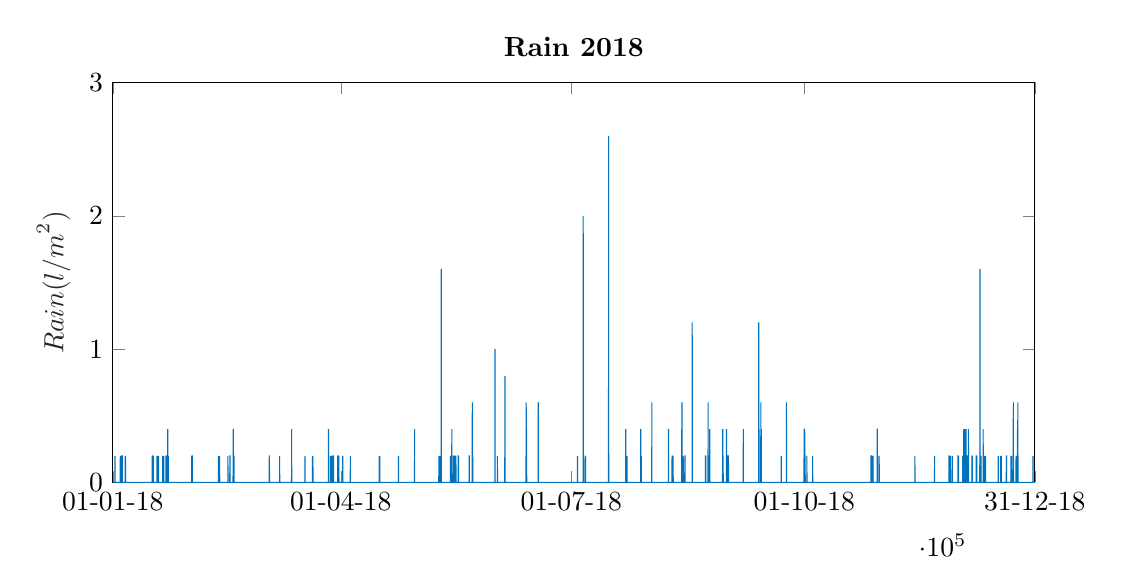
\begin{tikzpicture}

\begin{axis}[%
width=4.61in,
height=2in,
at={(0.758in,0.481in)},
scale only axis,
xmin=737061,
xmax=737425,
xtick={736969,737061,737151,737242,737334,737425},
xticklabels={{01-10-17},{01-01-18},{01-04-18},{01-07-18},{01-10-18},{31-12-18}},
ymin=0,
ymax=3,
ylabel style={font=\color{white!15!black}},
ylabel={$\text{Rain (l/m}^\text{2}\text{)}$},
axis background/.style={fill=white},
title style={font=\bfseries},
title={Rain 2018},
legend style={legend cell align=left, align=left, draw=white!15!black}
]
\addplot [color=mycolor1, forget plot]
  table[row sep=crcr]{%
737061	0\\
737061.034722222	0\\
737061.069444444	0\\
737061.104166667	0\\
737061.138888889	0\\
737061.173611111	0\\
737061.208333333	0\\
737061.243055556	0\\
737061.277777778	0\\
737061.3125	0\\
737061.347222222	0\\
737061.381944444	0\\
737061.416666667	0\\
737061.451388889	0\\
737061.486111111	0\\
737061.520833333	0\\
737061.555555556	0\\
737061.590277778	0\\
737061.625	0\\
737061.659722222	0\\
737061.694444444	0\\
737061.729166667	0\\
737061.763888889	0\\
737061.798611111	0\\
737061.833333333	0\\
737061.868055556	0.2\\
737061.902777778	0\\
737061.9375	0\\
737061.972222222	0\\
737062.006944444	0\\
737062.041666667	0\\
737062.076388889	0\\
737062.111111111	0\\
737062.145833333	0\\
737062.184027778	0\\
737062.21875	0\\
737062.253472222	0\\
737062.288194444	0\\
737062.322916667	0\\
737062.357638889	0\\
737062.392361111	0\\
737062.427083333	0\\
737062.461805556	0\\
737062.496527778	0\\
737062.53125	0\\
737062.565972222	0\\
737062.600694444	0\\
737062.635416667	0\\
737062.670138889	0\\
737062.704861111	0\\
737062.739583333	0\\
737062.774305556	0\\
737062.809027778	0\\
737062.84375	0\\
737062.878472222	0\\
737062.913194444	0\\
737062.947916667	0\\
737062.982638889	0\\
737063.017361111	0\\
737063.052083333	0\\
737063.086805556	0\\
737063.121527778	0\\
737063.15625	0\\
737063.190972222	0\\
737063.225694444	0\\
737063.260416667	0\\
737063.295138889	0\\
737063.329861111	0\\
737063.364583333	0\\
737063.399305556	0\\
737063.434027778	0\\
737063.46875	0\\
737063.503472222	0\\
737063.538194444	0\\
737063.572916667	0\\
737063.607638889	0\\
737063.642361111	0\\
737063.677083333	0\\
737063.711805556	0\\
737063.746527778	0\\
737063.78125	0\\
737063.815972222	0\\
737063.850694444	0\\
737063.885416667	0\\
737063.920138889	0\\
737063.954861111	0.2\\
737063.989583333	0\\
737064.027777778	0.2\\
737064.0625	0\\
737064.097222222	0\\
737064.131944444	0\\
737064.166666667	0\\
737064.201388889	0\\
737064.236111111	0\\
737064.270833333	0\\
737064.305555556	0\\
737064.34375	0\\
737064.378472222	0.2\\
737064.413194444	0\\
737064.447916667	0\\
737064.482638889	0.2\\
737064.517361111	0.2\\
737064.552083333	0.2\\
737064.586805556	0.2\\
737064.621527778	0.2\\
737064.65625	0\\
737064.690972222	0.2\\
737064.725694444	0.2\\
737064.760416667	0\\
737064.795138889	0\\
737064.829861111	0\\
737064.864583333	0\\
737064.899305556	0\\
737064.934027778	0\\
737064.96875	0\\
737065.003472222	0\\
737065.038194444	0\\
737065.072916667	0\\
737065.107638889	0\\
737065.142361111	0\\
737065.177083333	0\\
737065.211805556	0\\
737065.246527778	0\\
737065.28125	0\\
737065.315972222	0\\
737065.350694444	0\\
737065.385416667	0\\
737065.420138889	0\\
737065.454861111	0\\
737065.489583333	0\\
737065.524305556	0\\
737065.559027778	0\\
737065.59375	0\\
737065.628472222	0\\
737065.663194444	0\\
737065.697916667	0\\
737065.732638889	0\\
737065.767361111	0\\
737065.802083333	0\\
737065.836805556	0\\
737065.871527778	0\\
737065.90625	0.2\\
737065.940972222	0\\
737065.975694444	0.2\\
737066.013888889	0\\
737066.048611111	0\\
737066.083333333	0\\
737066.118055556	0\\
737066.152777778	0\\
737066.1875	0\\
737066.222222222	0\\
737066.256944444	0\\
737066.291666667	0\\
737066.326388889	0\\
737066.361111111	0\\
737066.395833333	0\\
737066.430555556	0\\
737066.465277778	0\\
737066.5	0\\
737066.534722222	0\\
737066.569444444	0\\
737066.604166667	0\\
737066.638888889	0\\
737066.673611111	0\\
737066.708333333	0\\
737066.743055556	0\\
737066.777777778	0\\
737066.8125	0\\
737066.847222222	0\\
737066.881944444	0\\
737066.916666667	0\\
737066.951388889	0\\
737066.986111111	0\\
737067.024305556	0\\
737067.059027778	0\\
737067.09375	0\\
737067.128472222	0\\
737067.163194444	0\\
737067.201388889	0\\
737067.236111111	0\\
737067.270833333	0\\
737067.305555556	0\\
737067.340277778	0\\
737067.375	0\\
737067.409722222	0\\
737067.444444444	0\\
737067.479166667	0\\
737067.513888889	0\\
737067.548611111	0\\
737067.583333333	0\\
737067.618055556	0\\
737067.652777778	0\\
737067.6875	0\\
737067.722222222	0\\
737067.756944444	0\\
737067.791666667	0\\
737067.826388889	0\\
737067.861111111	0\\
737067.895833333	0\\
737067.930555556	0\\
737067.965277778	0\\
737068	0\\
737068.034722222	0\\
737068.069444444	0\\
737068.104166667	0\\
737068.138888889	0\\
737068.173611111	0\\
737068.208333333	0\\
737068.243055556	0\\
737068.277777778	0\\
737068.3125	0\\
737068.347222222	0\\
737068.381944444	0\\
737068.416666667	0\\
737068.451388889	0\\
737068.486111111	0\\
737068.520833333	0\\
737068.555555556	0\\
737068.590277778	0\\
737068.625	0\\
737068.659722222	0\\
737068.694444444	0\\
737068.729166667	0\\
737068.763888889	0\\
737068.798611111	0\\
737068.833333333	0\\
737068.868055556	0\\
737068.902777778	0\\
737068.9375	0\\
737068.972222222	0\\
737069.010416667	0\\
737069.045138889	0\\
737069.079861111	0\\
737069.114583333	0\\
737069.149305556	0\\
737069.1875	0\\
737069.222222222	0\\
737069.256944444	0\\
737069.291666667	0\\
737069.326388889	0\\
737069.361111111	0\\
737069.395833333	0\\
737069.430555556	0\\
737069.465277778	0\\
737069.5	0\\
737069.534722222	0\\
737069.569444444	0\\
737069.604166667	0\\
737069.638888889	0\\
737069.673611111	0\\
737069.708333333	0\\
737069.743055556	0\\
737069.777777778	0\\
737069.8125	0\\
737069.847222222	0\\
737069.881944444	0\\
737069.916666667	0\\
737069.951388889	0\\
737069.986111111	0\\
737070.020833333	0\\
737070.055555556	0\\
737070.090277778	0\\
737070.125	0\\
737070.159722222	0\\
737070.197916667	0\\
737070.232638889	0\\
737070.267361111	0\\
737070.302083333	0\\
737070.336805556	0\\
737070.371527778	0\\
737070.40625	0\\
737070.440972222	0\\
737070.475694444	0\\
737070.510416667	0\\
737070.545138889	0\\
737070.579861111	0\\
737070.614583333	0\\
737070.649305556	0\\
737070.684027778	0\\
737070.71875	0\\
737070.753472222	0\\
737070.788194444	0\\
737070.822916667	0\\
737070.857638889	0\\
737070.892361111	0\\
737070.927083333	0\\
737070.961805556	0\\
737070.996527778	0\\
737071.03125	0\\
737071.065972222	0\\
737071.100694444	0\\
737071.135416667	0\\
737071.173611111	0\\
737071.208333333	0\\
737071.243055556	0\\
737071.277777778	0\\
737071.3125	0\\
737071.347222222	0\\
737071.381944444	0\\
737071.416666667	0\\
737071.451388889	0\\
737071.486111111	0\\
737071.520833333	0\\
737071.555555556	0\\
737071.590277778	0\\
737071.625	0\\
737071.659722222	0\\
737071.694444444	0\\
737071.729166667	0\\
737071.763888889	0\\
737071.798611111	0\\
737071.833333333	0\\
737071.868055556	0\\
737071.902777778	0\\
737071.9375	0\\
737071.972222222	0\\
737072.006944444	0\\
737072.041666667	0\\
737072.076388889	0\\
737072.111111111	0\\
737072.145833333	0\\
737072.184027778	0\\
737072.21875	0\\
737072.253472222	0\\
737072.288194444	0\\
737072.322916667	0\\
737072.357638889	0\\
737072.392361111	0\\
737072.427083333	0\\
737072.461805556	0\\
737072.496527778	0\\
737072.53125	0\\
737072.565972222	0\\
737072.600694444	0\\
737072.635416667	0\\
737072.670138889	0\\
737072.704861111	0\\
737072.739583333	0\\
737072.774305556	0\\
737072.809027778	0\\
737072.84375	0\\
737072.878472222	0\\
737072.913194444	0\\
737072.947916667	0\\
737072.982638889	0\\
737073.017361111	0\\
737073.052083333	0\\
737073.086805556	0\\
737073.121527778	0\\
737073.15625	0\\
737073.194444444	0\\
737073.229166667	0\\
737073.263888889	0\\
737073.298611111	0\\
737073.333333333	0\\
737073.368055556	0\\
737073.402777778	0\\
737073.4375	0\\
737073.472222222	0\\
737073.506944444	0\\
737073.541666667	0\\
737073.576388889	0\\
737073.611111111	0\\
737073.645833333	0\\
737073.680555556	0\\
737073.715277778	0\\
737073.75	0\\
737073.784722222	0\\
737073.819444444	0\\
737073.854166667	0\\
737073.888888889	0\\
737073.923611111	0\\
737073.958333333	0\\
737073.993055556	0\\
737074.027777778	0\\
737074.0625	0\\
737074.097222222	0\\
737074.131944444	0\\
737074.166666667	0\\
737074.204861111	0\\
737074.239583333	0\\
737074.274305556	0\\
737074.309027778	0\\
737074.34375	0\\
737074.378472222	0\\
737074.413194444	0\\
737074.447916667	0\\
737074.482638889	0\\
737074.517361111	0\\
737074.552083333	0\\
737074.586805556	0\\
737074.621527778	0\\
737074.65625	0\\
737074.690972222	0\\
737074.725694444	0\\
737074.760416667	0\\
737074.795138889	0\\
737074.829861111	0\\
737074.864583333	0\\
737074.899305556	0\\
737074.934027778	0\\
737074.96875	0\\
737075.003472222	0\\
737075.038194444	0\\
737075.072916667	0\\
737075.107638889	0\\
737075.142361111	0\\
737075.177083333	0\\
737075.211805556	0\\
737075.246527778	0\\
737075.28125	0\\
737075.315972222	0\\
737075.350694444	0\\
737075.385416667	0\\
737075.420138889	0\\
737075.454861111	0\\
737075.489583333	0\\
737075.524305556	0\\
737075.559027778	0\\
737075.59375	0\\
737075.628472222	0\\
737075.663194444	0\\
737075.697916667	0\\
737075.732638889	0\\
737075.767361111	0\\
737075.802083333	0\\
737075.836805556	0\\
737075.871527778	0\\
737075.90625	0\\
737075.940972222	0\\
737075.975694444	0\\
737076.013888889	0\\
737076.048611111	0\\
737076.083333333	0\\
737076.118055556	0\\
737076.152777778	0\\
737076.190972222	0\\
737076.225694444	0\\
737076.260416667	0\\
737076.295138889	0\\
737076.329861111	0\\
737076.364583333	0\\
737076.399305556	0\\
737076.434027778	0\\
737076.46875	0\\
737076.503472222	0\\
737076.538194444	0.2\\
737076.572916667	0\\
737076.607638889	0\\
737076.642361111	0\\
737076.677083333	0.2\\
737076.711805556	0.2\\
737076.746527778	0\\
737076.78125	0.2\\
737076.815972222	0\\
737076.850694444	0\\
737076.885416667	0\\
737076.920138889	0\\
737076.954861111	0.2\\
737076.989583333	0\\
737077.024305556	0\\
737077.059027778	0\\
737077.09375	0\\
737077.128472222	0\\
737077.163194444	0\\
737077.197916667	0\\
737077.232638889	0\\
737077.267361111	0\\
737077.302083333	0\\
737077.336805556	0\\
737077.371527778	0\\
737077.40625	0\\
737077.440972222	0\\
737077.475694444	0\\
737077.510416667	0\\
737077.545138889	0\\
737077.579861111	0\\
737077.614583333	0\\
737077.649305556	0\\
737077.684027778	0\\
737077.71875	0\\
737077.753472222	0\\
737077.788194444	0\\
737077.822916667	0\\
737077.857638889	0\\
737077.892361111	0\\
737077.927083333	0\\
737077.961805556	0\\
737078	0\\
737078.034722222	0\\
737078.069444444	0\\
737078.104166667	0\\
737078.138888889	0\\
737078.173611111	0\\
737078.208333333	0\\
737078.243055556	0\\
737078.277777778	0\\
737078.3125	0\\
737078.347222222	0\\
737078.381944444	0\\
737078.416666667	0.2\\
737078.451388889	0\\
737078.486111111	0.2\\
737078.520833333	0\\
737078.555555556	0\\
737078.590277778	0\\
737078.625	0\\
737078.659722222	0\\
737078.694444444	0\\
737078.729166667	0\\
737078.763888889	0\\
737078.798611111	0\\
737078.833333333	0\\
737078.868055556	0\\
737078.902777778	0\\
737078.9375	0\\
737078.972222222	0\\
737079.010416667	0.2\\
737079.045138889	0\\
737079.079861111	0\\
737079.114583333	0\\
737079.149305556	0\\
737079.1875	0\\
737079.222222222	0\\
737079.256944444	0\\
737079.291666667	0\\
737079.326388889	0\\
737079.361111111	0\\
737079.395833333	0\\
737079.430555556	0\\
737079.465277778	0\\
737079.5	0\\
737079.534722222	0\\
737079.569444444	0\\
737079.604166667	0\\
737079.638888889	0\\
737079.673611111	0\\
737079.708333333	0\\
737079.743055556	0\\
737079.777777778	0\\
737079.8125	0\\
737079.847222222	0\\
737079.881944444	0\\
737079.916666667	0\\
737079.951388889	0\\
737079.986111111	0\\
737080.020833333	0\\
737080.055555556	0\\
737080.090277778	0\\
737080.125	0\\
737080.159722222	0\\
737080.197916667	0\\
737080.232638889	0\\
737080.267361111	0\\
737080.302083333	0\\
737080.336805556	0\\
737080.371527778	0\\
737080.40625	0\\
737080.440972222	0\\
737080.475694444	0\\
737080.510416667	0\\
737080.545138889	0\\
737080.579861111	0\\
737080.614583333	0\\
737080.649305556	0\\
737080.684027778	0\\
737080.71875	0.2\\
737080.753472222	0\\
737080.788194444	0\\
737080.822916667	0\\
737080.857638889	0.2\\
737080.892361111	0\\
737080.927083333	0\\
737080.961805556	0.2\\
737080.996527778	0\\
737081.03125	0\\
737081.065972222	0\\
737081.100694444	0\\
737081.135416667	0.2\\
737081.170138889	0\\
737081.204861111	0\\
737081.239583333	0\\
737081.274305556	0\\
737081.309027778	0\\
737081.34375	0\\
737081.378472222	0\\
737081.413194444	0\\
737081.447916667	0\\
737081.482638889	0\\
737081.517361111	0\\
737081.552083333	0\\
737081.586805556	0\\
737081.621527778	0\\
737081.65625	0\\
737081.690972222	0\\
737081.725694444	0\\
737081.760416667	0\\
737081.795138889	0\\
737081.829861111	0\\
737081.864583333	0\\
737081.899305556	0\\
737081.934027778	0\\
737081.96875	0.2\\
737082.006944444	0\\
737082.041666667	0.2\\
737082.076388889	0.2\\
737082.111111111	0.2\\
737082.145833333	0.2\\
737082.180555556	0.2\\
737082.215277778	0\\
737082.25	0\\
737082.284722222	0\\
737082.319444444	0\\
737082.354166667	0\\
737082.388888889	0\\
737082.423611111	0\\
737082.458333333	0\\
737082.493055556	0.2\\
737082.527777778	0\\
737082.5625	0\\
737082.597222222	0.2\\
737082.631944444	0\\
737082.666666667	0.2\\
737082.701388889	0.4\\
737082.736111111	0.2\\
737082.770833333	0\\
737082.805555556	0\\
737082.840277778	0\\
737082.875	0.2\\
737082.909722222	0\\
737082.944444444	0\\
737082.979166667	0\\
737083.017361111	0\\
737083.052083333	0\\
737083.086805556	0\\
737083.121527778	0\\
737083.15625	0\\
737083.190972222	0\\
737083.225694444	0\\
737083.260416667	0\\
737083.295138889	0\\
737083.329861111	0\\
737083.364583333	0\\
737083.399305556	0\\
737083.434027778	0\\
737083.46875	0\\
737083.503472222	0\\
737083.538194444	0\\
737083.572916667	0\\
737083.607638889	0\\
737083.642361111	0\\
737083.677083333	0\\
737083.711805556	0\\
737083.746527778	0\\
737083.78125	0\\
737083.815972222	0\\
737083.850694444	0\\
737083.885416667	0\\
737083.920138889	0\\
737083.954861111	0\\
737083.989583333	0\\
737084.027777778	0\\
737084.0625	0\\
737084.097222222	0\\
737084.131944444	0\\
737084.166666667	0\\
737084.204861111	0\\
737084.239583333	0\\
737084.274305556	0\\
737084.309027778	0\\
737084.34375	0\\
737084.378472222	0\\
737084.413194444	0\\
737084.447916667	0\\
737084.482638889	0\\
737084.517361111	0\\
737084.552083333	0\\
737084.586805556	0\\
737084.621527778	0\\
737084.65625	0\\
737084.690972222	0\\
737084.725694444	0\\
737084.760416667	0\\
737084.795138889	0\\
737084.829861111	0\\
737084.864583333	0\\
737084.899305556	0\\
737084.934027778	0\\
737084.96875	0\\
737085.003472222	0\\
737085.038194444	0\\
737085.072916667	0\\
737085.107638889	0\\
737085.142361111	0\\
737085.180555556	0\\
737085.215277778	0\\
737085.25	0\\
737085.284722222	0\\
737085.319444444	0\\
737085.354166667	0\\
737085.388888889	0\\
737085.423611111	0\\
737085.458333333	0\\
737085.493055556	0\\
737085.527777778	0\\
737085.5625	0\\
737085.597222222	0\\
737085.631944444	0\\
737085.666666667	0\\
737085.701388889	0\\
737085.736111111	0\\
737085.770833333	0\\
737085.805555556	0\\
737085.840277778	0\\
737085.875	0\\
737085.909722222	0\\
737085.944444444	0\\
737085.979166667	0\\
737086.013888889	0\\
737086.048611111	0\\
737086.083333333	0\\
737086.118055556	0\\
737086.152777778	0\\
737086.190972222	0\\
737086.225694444	0\\
737086.260416667	0\\
737086.295138889	0\\
737086.329861111	0\\
737086.364583333	0\\
737086.399305556	0\\
737086.434027778	0\\
737086.46875	0\\
737086.506944444	0\\
737086.541666667	0\\
737086.576388889	0\\
737086.611111111	0\\
737086.645833333	0\\
737086.680555556	0\\
737086.715277778	0\\
737086.75	0\\
737086.784722222	0\\
737086.819444444	0\\
737086.854166667	0\\
737086.888888889	0\\
737086.923611111	0\\
737086.958333333	0\\
737086.993055556	0\\
737087.027777778	0\\
737087.0625	0\\
737087.097222222	0\\
737087.131944444	0\\
737087.166666667	0\\
737087.204861111	0\\
737087.239583333	0\\
737087.274305556	0\\
737087.309027778	0\\
737087.34375	0\\
737087.378472222	0\\
737087.413194444	0\\
737087.447916667	0\\
737087.482638889	0\\
737087.517361111	0\\
737087.552083333	0\\
737087.586805556	0\\
737087.621527778	0\\
737087.65625	0\\
737087.690972222	0\\
737087.725694444	0\\
737087.760416667	0\\
737087.795138889	0\\
737087.829861111	0\\
737087.864583333	0\\
737087.899305556	0\\
737087.934027778	0\\
737087.96875	0\\
737088.003472222	0\\
737088.038194444	0\\
737088.072916667	0\\
737088.107638889	0\\
737088.142361111	0\\
737088.180555556	0\\
737088.215277778	0\\
737088.25	0\\
737088.284722222	0\\
737088.319444444	0\\
737088.354166667	0\\
737088.388888889	0\\
737088.423611111	0\\
737088.458333333	0\\
737088.493055556	0\\
737088.527777778	0\\
737088.5625	0\\
737088.597222222	0\\
737088.631944444	0\\
737088.666666667	0\\
737088.701388889	0\\
737088.736111111	0\\
737088.770833333	0\\
737088.805555556	0\\
737088.840277778	0\\
737088.875	0\\
737088.909722222	0\\
737088.944444444	0\\
737088.979166667	0\\
737089.013888889	0\\
737089.048611111	0\\
737089.083333333	0\\
737089.118055556	0\\
737089.152777778	0\\
737089.190972222	0\\
737089.225694444	0\\
737089.260416667	0\\
737089.295138889	0\\
737089.329861111	0\\
737089.364583333	0\\
737089.399305556	0\\
737089.434027778	0\\
737089.46875	0\\
737089.503472222	0\\
737089.538194444	0\\
737089.572916667	0\\
737089.607638889	0\\
737089.642361111	0\\
737089.677083333	0\\
737089.711805556	0\\
737089.746527778	0\\
737089.78125	0\\
737089.815972222	0\\
737089.850694444	0\\
737089.885416667	0\\
737089.920138889	0\\
737089.954861111	0\\
737089.989583333	0\\
737090.024305556	0\\
737090.059027778	0\\
737090.09375	0\\
737090.128472222	0\\
737090.163194444	0\\
737090.197916667	0\\
737090.232638889	0\\
737090.267361111	0\\
737090.302083333	0\\
737090.336805556	0\\
737090.371527778	0\\
737090.40625	0\\
737090.440972222	0\\
737090.475694444	0\\
737090.510416667	0\\
737090.545138889	0\\
737090.579861111	0\\
737090.614583333	0\\
737090.649305556	0\\
737090.684027778	0\\
737090.71875	0\\
737090.753472222	0\\
737090.788194444	0\\
737090.822916667	0\\
737090.857638889	0\\
737090.892361111	0\\
737090.927083333	0\\
737090.961805556	0\\
737091	0\\
737091.034722222	0\\
737091.069444444	0\\
737091.104166667	0\\
737091.138888889	0\\
737091.173611111	0\\
737091.208333333	0\\
737091.243055556	0\\
737091.277777778	0\\
737091.3125	0\\
737091.347222222	0\\
737091.381944444	0\\
737091.416666667	0\\
737091.451388889	0\\
737091.486111111	0\\
737091.520833333	0\\
737091.555555556	0\\
737091.590277778	0\\
737091.625	0\\
737091.659722222	0\\
737091.694444444	0\\
737091.729166667	0\\
737091.763888889	0\\
737091.798611111	0\\
737091.833333333	0\\
737091.868055556	0\\
737091.902777778	0\\
737091.9375	0\\
737091.972222222	0\\
737092.010416667	0\\
737092.045138889	0\\
737092.079861111	0\\
737092.114583333	0.2\\
737092.149305556	0\\
737092.184027778	0\\
737092.21875	0.2\\
737092.253472222	0\\
737092.288194444	0.2\\
737092.322916667	0.2\\
737092.357638889	0.2\\
737092.392361111	0.2\\
737092.427083333	0\\
737092.461805556	0\\
737092.496527778	0\\
737092.53125	0\\
737092.565972222	0\\
737092.600694444	0\\
737092.635416667	0\\
737092.670138889	0\\
737092.704861111	0\\
737092.739583333	0\\
737092.774305556	0\\
737092.809027778	0\\
737092.84375	0\\
737092.878472222	0\\
737092.913194444	0\\
737092.947916667	0\\
737092.982638889	0\\
737093.020833333	0\\
737093.055555556	0\\
737093.090277778	0\\
737093.125	0\\
737093.159722222	0\\
737093.197916667	0\\
737093.232638889	0\\
737093.267361111	0\\
737093.302083333	0\\
737093.336805556	0\\
737093.371527778	0\\
737093.40625	0\\
737093.440972222	0\\
737093.475694444	0\\
737093.510416667	0\\
737093.545138889	0\\
737093.579861111	0\\
737093.614583333	0\\
737093.649305556	0\\
737093.684027778	0\\
737093.71875	0\\
737093.753472222	0\\
737093.788194444	0\\
737093.822916667	0\\
737093.857638889	0\\
737093.892361111	0\\
737093.927083333	0\\
737093.961805556	0\\
737093.996527778	0\\
737094.03125	0\\
737094.065972222	0\\
737094.100694444	0\\
737094.135416667	0\\
737094.173611111	0\\
737094.208333333	0\\
737094.243055556	0\\
737094.277777778	0\\
737094.3125	0\\
737094.347222222	0\\
737094.381944444	0\\
737094.416666667	0\\
737094.451388889	0\\
737094.486111111	0\\
737094.520833333	0\\
737094.555555556	0\\
737094.590277778	0\\
737094.625	0\\
737094.659722222	0\\
737094.694444444	0\\
737094.729166667	0\\
737094.763888889	0\\
737094.798611111	0\\
737094.833333333	0\\
737094.868055556	0\\
737094.902777778	0\\
737094.9375	0\\
737094.972222222	0\\
737095.006944444	0\\
737095.041666667	0\\
737095.076388889	0\\
737095.111111111	0\\
737095.145833333	0\\
737095.184027778	0\\
737095.21875	0\\
737095.253472222	0\\
737095.288194444	0\\
737095.322916667	0\\
737095.357638889	0\\
737095.392361111	0\\
737095.427083333	0\\
737095.461805556	0\\
737095.496527778	0\\
737095.53125	0\\
737095.565972222	0\\
737095.600694444	0\\
737095.635416667	0\\
737095.670138889	0\\
737095.704861111	0\\
737095.739583333	0\\
737095.774305556	0\\
737095.809027778	0\\
737095.84375	0\\
737095.878472222	0\\
737095.913194444	0\\
737095.947916667	0\\
737095.982638889	0\\
737096.017361111	0\\
737096.052083333	0\\
737096.086805556	0\\
737096.121527778	0\\
737096.15625	0\\
737096.190972222	0\\
737096.225694444	0\\
737096.260416667	0\\
737096.295138889	0\\
737096.329861111	0\\
737096.364583333	0\\
737096.399305556	0\\
737096.434027778	0\\
737096.46875	0\\
737096.503472222	0\\
737096.538194444	0\\
737096.572916667	0\\
737096.607638889	0\\
737096.642361111	0\\
737096.677083333	0\\
737096.711805556	0\\
737096.746527778	0\\
737096.78125	0\\
737096.815972222	0\\
737096.850694444	0\\
737096.885416667	0\\
737096.920138889	0\\
737096.954861111	0\\
737096.989583333	0\\
737097.027777778	0\\
737097.0625	0\\
737097.097222222	0\\
737097.131944444	0\\
737097.166666667	0\\
737097.204861111	0\\
737097.239583333	0\\
737097.274305556	0\\
737097.309027778	0\\
737097.34375	0\\
737097.378472222	0\\
737097.413194444	0\\
737097.447916667	0\\
737097.482638889	0\\
737097.517361111	0\\
737097.552083333	0\\
737097.586805556	0\\
737097.621527778	0\\
737097.65625	0\\
737097.690972222	0\\
737097.725694444	0\\
737097.760416667	0\\
737097.795138889	0\\
737097.829861111	0\\
737097.864583333	0\\
737097.899305556	0\\
737097.934027778	0\\
737097.96875	0\\
737098.003472222	0\\
737098.038194444	0\\
737098.072916667	0\\
737098.107638889	0\\
737098.142361111	0\\
737098.180555556	0\\
737098.215277778	0\\
737098.25	0\\
737098.284722222	0\\
737098.319444444	0\\
737098.354166667	0\\
737098.388888889	0\\
737098.423611111	0\\
737098.458333333	0\\
737098.493055556	0\\
737098.527777778	0\\
737098.5625	0\\
737098.597222222	0\\
737098.631944444	0\\
737098.666666667	0\\
737098.701388889	0\\
737098.736111111	0\\
737098.770833333	0\\
737098.805555556	0\\
737098.840277778	0\\
737098.875	0\\
737098.909722222	0\\
737098.944444444	0\\
737098.979166667	0\\
737099.013888889	0\\
737099.048611111	0\\
737099.083333333	0\\
737099.118055556	0\\
737099.152777778	0\\
737099.190972222	0\\
737099.225694444	0\\
737099.260416667	0\\
737099.295138889	0\\
737099.329861111	0\\
737099.364583333	0\\
737099.399305556	0\\
737099.434027778	0\\
737099.46875	0\\
737099.503472222	0\\
737099.538194444	0\\
737099.572916667	0\\
737099.607638889	0\\
737099.642361111	0\\
737099.677083333	0\\
737099.711805556	0\\
737099.746527778	0\\
737099.78125	0\\
737099.815972222	0\\
737099.850694444	0\\
737099.885416667	0\\
737099.920138889	0\\
737099.954861111	0\\
737099.989583333	0\\
737100.024305556	0\\
737100.059027778	0\\
737100.09375	0\\
737100.128472222	0\\
737100.163194444	0\\
737100.197916667	0\\
737100.232638889	0\\
737100.267361111	0\\
737100.302083333	0\\
737100.336805556	0\\
737100.371527778	0\\
737100.40625	0\\
737100.440972222	0\\
737100.475694444	0\\
737100.510416667	0\\
737100.545138889	0\\
737100.579861111	0\\
737100.614583333	0\\
737100.649305556	0\\
737100.684027778	0\\
737100.71875	0\\
737100.753472222	0\\
737100.788194444	0\\
737100.822916667	0\\
737100.857638889	0\\
737100.892361111	0\\
737100.927083333	0\\
737100.961805556	0\\
737101	0\\
737101.034722222	0\\
737101.069444444	0\\
737101.104166667	0\\
737101.138888889	0\\
737101.177083333	0\\
737101.211805556	0\\
737101.246527778	0\\
737101.28125	0\\
737101.315972222	0\\
737101.350694444	0\\
737101.385416667	0\\
737101.420138889	0\\
737101.454861111	0\\
737101.489583333	0\\
737101.524305556	0\\
737101.559027778	0\\
737101.59375	0\\
737101.628472222	0\\
737101.663194444	0\\
737101.697916667	0\\
737101.732638889	0\\
737101.767361111	0\\
737101.802083333	0\\
737101.836805556	0\\
737101.871527778	0\\
737101.90625	0\\
737101.940972222	0\\
737101.975694444	0\\
737102.010416667	0\\
737102.045138889	0\\
737102.079861111	0\\
737102.114583333	0\\
737102.149305556	0\\
737102.184027778	0\\
737102.21875	0\\
737102.253472222	0\\
737102.288194444	0\\
737102.322916667	0\\
737102.357638889	0\\
737102.392361111	0\\
737102.427083333	0\\
737102.461805556	0\\
737102.496527778	0\\
737102.53125	0\\
737102.565972222	0\\
737102.600694444	0\\
737102.635416667	0\\
737102.670138889	0\\
737102.704861111	0.2\\
737102.739583333	0\\
737102.774305556	0\\
737102.809027778	0\\
737102.84375	0\\
737102.878472222	0\\
737102.913194444	0\\
737102.947916667	0\\
737102.982638889	0.2\\
737103.020833333	0\\
737103.055555556	0\\
737103.090277778	0.2\\
737103.125	0\\
737103.159722222	0.2\\
737103.197916667	0\\
737103.232638889	0\\
737103.267361111	0\\
737103.302083333	0\\
737103.336805556	0\\
737103.371527778	0\\
737103.40625	0\\
737103.440972222	0\\
737103.475694444	0\\
737103.510416667	0\\
737103.545138889	0\\
737103.579861111	0\\
737103.614583333	0\\
737103.649305556	0\\
737103.684027778	0\\
737103.71875	0\\
737103.753472222	0\\
737103.788194444	0\\
737103.822916667	0\\
737103.857638889	0\\
737103.892361111	0\\
737103.927083333	0\\
737103.961805556	0\\
737103.996527778	0\\
737104.03125	0\\
737104.065972222	0\\
737104.100694444	0\\
737104.135416667	0\\
737104.170138889	0\\
737104.204861111	0\\
737104.239583333	0\\
737104.274305556	0\\
737104.309027778	0\\
737104.34375	0\\
737104.378472222	0\\
737104.413194444	0\\
737104.447916667	0\\
737104.482638889	0\\
737104.517361111	0\\
737104.552083333	0\\
737104.586805556	0\\
737104.621527778	0\\
737104.65625	0\\
737104.690972222	0\\
737104.725694444	0\\
737104.760416667	0\\
737104.795138889	0\\
737104.829861111	0\\
737104.864583333	0\\
737104.899305556	0\\
737104.934027778	0\\
737104.96875	0\\
737105.006944444	0\\
737105.041666667	0\\
737105.076388889	0\\
737105.111111111	0\\
737105.145833333	0\\
737105.180555556	0\\
737105.215277778	0\\
737105.25	0\\
737105.284722222	0\\
737105.319444444	0\\
737105.354166667	0\\
737105.388888889	0\\
737105.423611111	0\\
737105.458333333	0\\
737105.493055556	0\\
737105.527777778	0\\
737105.5625	0\\
737105.597222222	0\\
737105.631944444	0\\
737105.666666667	0\\
737105.701388889	0\\
737105.736111111	0\\
737105.770833333	0\\
737105.805555556	0\\
737105.840277778	0\\
737105.875	0\\
737105.909722222	0\\
737105.944444444	0\\
737105.979166667	0\\
737106.017361111	0\\
737106.052083333	0\\
737106.086805556	0\\
737106.121527778	0\\
737106.15625	0\\
737106.190972222	0\\
737106.225694444	0\\
737106.260416667	0\\
737106.295138889	0\\
737106.329861111	0\\
737106.364583333	0\\
737106.399305556	0\\
737106.434027778	0.2\\
737106.46875	0\\
737106.503472222	0\\
737106.538194444	0\\
737106.572916667	0\\
737106.607638889	0\\
737106.642361111	0\\
737106.677083333	0\\
737106.711805556	0\\
737106.746527778	0\\
737106.78125	0\\
737106.815972222	0\\
737106.850694444	0\\
737106.885416667	0\\
737106.920138889	0\\
737106.954861111	0\\
737106.989583333	0\\
737107.027777778	0\\
737107.0625	0\\
737107.097222222	0\\
737107.131944444	0\\
737107.166666667	0\\
737107.204861111	0.2\\
737107.239583333	0.2\\
737107.274305556	0.2\\
737107.309027778	0\\
737107.34375	0\\
737107.378472222	0\\
737107.413194444	0\\
737107.447916667	0\\
737107.482638889	0\\
737107.517361111	0\\
737107.552083333	0\\
737107.586805556	0\\
737107.621527778	0\\
737107.65625	0\\
737107.690972222	0\\
737107.725694444	0\\
737107.760416667	0\\
737107.795138889	0\\
737107.829861111	0\\
737107.864583333	0\\
737107.899305556	0\\
737107.934027778	0\\
737107.96875	0\\
737108.003472222	0\\
737108.038194444	0\\
737108.072916667	0\\
737108.107638889	0\\
737108.142361111	0\\
737108.177083333	0\\
737108.211805556	0\\
737108.246527778	0\\
737108.28125	0\\
737108.315972222	0\\
737108.350694444	0\\
737108.385416667	0\\
737108.420138889	0\\
737108.454861111	0\\
737108.489583333	0.2\\
737108.524305556	0.4\\
737108.559027778	0\\
737108.59375	0\\
737108.628472222	0.2\\
737108.663194444	0\\
737108.697916667	0.2\\
737108.732638889	0.2\\
737108.767361111	0.2\\
737108.802083333	0.2\\
737108.836805556	0\\
737108.871527778	0.2\\
737108.90625	0\\
737108.940972222	0\\
737108.975694444	0\\
737109.013888889	0\\
737109.048611111	0\\
737109.083333333	0\\
737109.118055556	0\\
737109.152777778	0\\
737109.1875	0\\
737109.222222222	0\\
737109.256944444	0\\
737109.291666667	0\\
737109.326388889	0\\
737109.361111111	0\\
737109.395833333	0\\
737109.430555556	0\\
737109.465277778	0\\
737109.5	0\\
737109.534722222	0\\
737109.569444444	0\\
737109.604166667	0\\
737109.638888889	0\\
737109.673611111	0\\
737109.708333333	0\\
737109.743055556	0\\
737109.777777778	0\\
737109.8125	0\\
737109.847222222	0\\
737109.881944444	0\\
737109.916666667	0\\
737109.951388889	0\\
737109.986111111	0\\
737110.024305556	0\\
737110.059027778	0\\
737110.09375	0\\
737110.128472222	0\\
737110.163194444	0\\
737110.201388889	0\\
737110.236111111	0\\
737110.270833333	0\\
737110.305555556	0\\
737110.340277778	0\\
737110.375	0\\
737110.409722222	0\\
737110.444444444	0\\
737110.479166667	0\\
737110.513888889	0\\
737110.548611111	0\\
737110.583333333	0\\
737110.618055556	0\\
737110.652777778	0\\
737110.6875	0\\
737110.722222222	0\\
737110.756944444	0\\
737110.791666667	0\\
737110.826388889	0\\
737110.861111111	0\\
737110.895833333	0\\
737110.930555556	0\\
737110.965277778	0\\
737111	0\\
737111.034722222	0\\
737111.069444444	0\\
737111.104166667	0\\
737111.138888889	0\\
737111.173611111	0\\
737111.208333333	0\\
737111.243055556	0\\
737111.277777778	0\\
737111.3125	0\\
737111.347222222	0\\
737111.381944444	0\\
737111.416666667	0\\
737111.451388889	0\\
737111.486111111	0\\
737111.520833333	0\\
737111.555555556	0\\
737111.590277778	0\\
737111.625	0\\
737111.659722222	0\\
737111.694444444	0\\
737111.729166667	0\\
737111.763888889	0\\
737111.798611111	0\\
737111.833333333	0\\
737111.868055556	0\\
737111.902777778	0\\
737111.9375	0\\
737111.972222222	0\\
737112.010416667	0\\
737112.045138889	0\\
737112.079861111	0\\
737112.114583333	0\\
737112.149305556	0\\
737112.1875	0\\
737112.222222222	0\\
737112.256944444	0\\
737112.291666667	0\\
737112.326388889	0\\
737112.361111111	0\\
737112.395833333	0\\
737112.430555556	0\\
737112.465277778	0\\
737112.5	0\\
737112.534722222	0\\
737112.569444444	0\\
737112.604166667	0\\
737112.638888889	0\\
737112.673611111	0\\
737112.708333333	0\\
737112.743055556	0\\
737112.777777778	0\\
737112.8125	0\\
737112.847222222	0\\
737112.881944444	0\\
737112.916666667	0\\
737112.951388889	0\\
737112.986111111	0\\
737113.020833333	0\\
737113.055555556	0\\
737113.090277778	0\\
737113.125	0\\
737113.159722222	0\\
737113.197916667	0\\
737113.232638889	0\\
737113.267361111	0\\
737113.302083333	0\\
737113.336805556	0\\
737113.371527778	0\\
737113.40625	0\\
737113.440972222	0\\
737113.475694444	0\\
737113.510416667	0\\
737113.545138889	0\\
737113.579861111	0\\
737113.614583333	0\\
737113.649305556	0\\
737113.684027778	0\\
737113.71875	0\\
737113.753472222	0\\
737113.788194444	0\\
737113.822916667	0\\
737113.857638889	0\\
737113.892361111	0\\
737113.927083333	0\\
737113.961805556	0\\
737113.996527778	0\\
737114.03125	0\\
737114.065972222	0\\
737114.100694444	0\\
737114.135416667	0\\
737114.174305556	0\\
737114.208333333	0\\
737114.243055556	0\\
737114.277777778	0\\
737114.3125	0\\
737114.347222222	0\\
737114.381944444	0\\
737114.416666667	0\\
737114.451388889	0\\
737114.486111111	0\\
737114.520833333	0\\
737114.555555556	0\\
737114.590277778	0\\
737114.625	0\\
737114.659722222	0\\
737114.694444444	0\\
737114.729166667	0\\
737114.763888889	0\\
737114.798611111	0\\
737114.833333333	0\\
737114.868055556	0\\
737114.902777778	0\\
737114.9375	0\\
737114.972222222	0\\
737115.006944444	0\\
737115.041666667	0\\
737115.076388889	0\\
737115.111111111	0\\
737115.145833333	0\\
737115.180555556	0\\
737115.215277778	0\\
737115.25	0\\
737115.284722222	0\\
737115.319444444	0\\
737115.354166667	0\\
737115.388888889	0\\
737115.423611111	0\\
737115.458333333	0\\
737115.493055556	0\\
737115.527777778	0\\
737115.5625	0\\
737115.597222222	0\\
737115.631944444	0\\
737115.666666667	0\\
737115.701388889	0\\
737115.736111111	0\\
737115.770833333	0\\
737115.805555556	0\\
737115.840277778	0\\
737115.875	0\\
737115.909722222	0\\
737115.944444444	0\\
737115.979166667	0\\
737116.017361111	0\\
737116.052083333	0\\
737116.086805556	0\\
737116.121527778	0\\
737116.15625	0\\
737116.194444444	0\\
737116.229166667	0\\
737116.263888889	0\\
737116.298611111	0\\
737116.333333333	0\\
737116.368055556	0\\
737116.402777778	0\\
737116.4375	0\\
737116.472222222	0\\
737116.506944444	0\\
737116.541666667	0\\
737116.576388889	0\\
737116.611111111	0\\
737116.645833333	0\\
737116.680555556	0\\
737116.715277778	0\\
737116.75	0\\
737116.784722222	0\\
737116.819444444	0\\
737116.854166667	0\\
737116.888888889	0\\
737116.923611111	0\\
737116.958333333	0\\
737116.993055556	0\\
737117.027777778	0\\
737117.0625	0\\
737117.097222222	0\\
737117.131944444	0\\
737117.166666667	0\\
737117.204861111	0\\
737117.239583333	0\\
737117.274305556	0\\
737117.309027778	0\\
737117.34375	0\\
737117.378472222	0\\
737117.413194444	0\\
737117.447916667	0\\
737117.482638889	0\\
737117.517361111	0\\
737117.552083333	0\\
737117.586805556	0\\
737117.621527778	0\\
737117.65625	0\\
737117.690972222	0\\
737117.725694444	0\\
737117.760416667	0\\
737117.795138889	0\\
737117.829861111	0\\
737117.864583333	0\\
737117.899305556	0\\
737117.934027778	0\\
737117.96875	0\\
737118.003472222	0\\
737118.038194444	0\\
737118.072916667	0\\
737118.107638889	0\\
737118.142361111	0\\
737118.180555556	0\\
737118.215277778	0\\
737118.25	0\\
737118.284722222	0\\
737118.319444444	0\\
737118.354166667	0\\
737118.388888889	0\\
737118.423611111	0\\
737118.458333333	0\\
737118.493055556	0\\
737118.527777778	0\\
737118.5625	0\\
737118.597222222	0\\
737118.631944444	0\\
737118.666666667	0\\
737118.701388889	0\\
737118.736111111	0\\
737118.770833333	0\\
737118.805555556	0\\
737118.840277778	0\\
737118.875	0\\
737118.909722222	0\\
737118.944444444	0\\
737118.979166667	0\\
737119.013888889	0\\
737119.048611111	0\\
737119.083333333	0\\
737119.118055556	0\\
737119.152777778	0\\
737119.1875	0\\
737119.222222222	0\\
737119.256944444	0\\
737119.291666667	0\\
737119.326388889	0\\
737119.361111111	0\\
737119.395833333	0\\
737119.430555556	0\\
737119.465277778	0\\
737119.5	0\\
737119.534722222	0\\
737119.569444444	0\\
737119.604166667	0\\
737119.638888889	0\\
737119.673611111	0\\
737119.708333333	0\\
737119.743055556	0\\
737119.777777778	0\\
737119.8125	0\\
737119.847222222	0\\
737119.881944444	0\\
737119.916666667	0\\
737119.951388889	0\\
737119.986111111	0\\
737120.024305556	0\\
737120.059027778	0\\
737120.09375	0\\
737120.128472222	0\\
737120.163194444	0\\
737120.197916667	0\\
737120.232638889	0\\
737120.267361111	0\\
737120.302083333	0\\
737120.336805556	0\\
737120.371527778	0\\
737120.40625	0\\
737120.440972222	0\\
737120.475694444	0\\
737120.510416667	0\\
737120.545138889	0\\
737120.579861111	0\\
737120.614583333	0\\
737120.649305556	0\\
737120.684027778	0\\
737120.71875	0\\
737120.753472222	0\\
737120.788194444	0\\
737120.822916667	0\\
737120.857638889	0\\
737120.892361111	0\\
737120.927083333	0\\
737120.961805556	0\\
737121	0\\
737121.034722222	0\\
737121.069444444	0\\
737121.104166667	0\\
737121.138888889	0\\
737121.173611111	0\\
737121.208333333	0\\
737121.243055556	0\\
737121.277777778	0\\
737121.3125	0\\
737121.347222222	0\\
737121.381944444	0\\
737121.416666667	0\\
737121.451388889	0\\
737121.486111111	0\\
737121.520833333	0\\
737121.555555556	0\\
737121.590277778	0\\
737121.625	0\\
737121.659722222	0\\
737121.694444444	0\\
737121.729166667	0\\
737121.763888889	0\\
737121.798611111	0\\
737121.833333333	0\\
737121.868055556	0\\
737121.902777778	0\\
737121.9375	0\\
737121.972222222	0\\
737122.010416667	0\\
737122.045138889	0\\
737122.079861111	0\\
737122.114583333	0\\
737122.149305556	0\\
737122.1875	0\\
737122.222222222	0\\
737122.256944444	0\\
737122.291666667	0\\
737122.326388889	0\\
737122.361111111	0\\
737122.395833333	0\\
737122.430555556	0\\
737122.465277778	0\\
737122.5	0\\
737122.534722222	0\\
737122.569444444	0\\
737122.604166667	0\\
737122.638888889	0\\
737122.673611111	0\\
737122.708333333	0\\
737122.743055556	0\\
737122.777777778	0.2\\
737122.8125	0.2\\
737122.847222222	0\\
737122.881944444	0\\
737122.916666667	0\\
737122.951388889	0\\
737122.986111111	0\\
737123.020833333	0\\
737123.055555556	0\\
737123.090277778	0\\
737123.125	0\\
737123.159722222	0\\
737123.194444444	0\\
737123.229166667	0\\
737123.263888889	0\\
737123.298611111	0\\
737123.333333333	0\\
737123.368055556	0\\
737123.402777778	0\\
737123.4375	0\\
737123.472222222	0\\
737123.506944444	0\\
737123.541666667	0\\
737123.576388889	0\\
737123.611111111	0\\
737123.645833333	0\\
737123.680555556	0\\
737123.715277778	0\\
737123.75	0\\
737123.784722222	0\\
737123.819444444	0\\
737123.854166667	0\\
737123.888888889	0\\
737123.923611111	0\\
737123.958333333	0\\
737123.993055556	0\\
737124.03125	0\\
737124.065972222	0\\
737124.100694444	0\\
737124.135416667	0\\
737124.170138889	0\\
737124.204861111	0\\
737124.239583333	0\\
737124.274305556	0\\
737124.309027778	0\\
737124.34375	0\\
737124.378472222	0\\
737124.413194444	0\\
737124.447916667	0\\
737124.482638889	0\\
737124.517361111	0\\
737124.552083333	0\\
737124.586805556	0\\
737124.621527778	0\\
737124.65625	0\\
737124.690972222	0\\
737124.725694444	0\\
737124.760416667	0\\
737124.795138889	0\\
737124.829861111	0\\
737124.864583333	0\\
737124.899305556	0\\
737124.934027778	0\\
737124.96875	0\\
737125.006944444	0\\
737125.041666667	0\\
737125.076388889	0\\
737125.111111111	0\\
737125.145833333	0\\
737125.180555556	0\\
737125.215277778	0\\
737125.25	0\\
737125.284722222	0\\
737125.319444444	0\\
737125.354166667	0\\
737125.388888889	0\\
737125.423611111	0\\
737125.458333333	0\\
737125.493055556	0\\
737125.527777778	0\\
737125.5625	0\\
737125.597222222	0\\
737125.631944444	0\\
737125.666666667	0\\
737125.701388889	0\\
737125.736111111	0\\
737125.770833333	0\\
737125.805555556	0\\
737125.840277778	0\\
737125.875	0\\
737125.909722222	0\\
737125.944444444	0\\
737125.979166667	0\\
737126.017361111	0\\
737126.052083333	0\\
737126.086805556	0\\
737126.121527778	0\\
737126.15625	0\\
737126.194444444	0\\
737126.229166667	0\\
737126.263888889	0\\
737126.298611111	0\\
737126.333333333	0\\
737126.368055556	0\\
737126.402777778	0\\
737126.4375	0\\
737126.472222222	0\\
737126.506944444	0\\
737126.541666667	0\\
737126.576388889	0\\
737126.611111111	0\\
737126.645833333	0\\
737126.680555556	0\\
737126.715277778	0\\
737126.75	0\\
737126.784722222	0\\
737126.819444444	0\\
737126.854166667	0.2\\
737126.888888889	0\\
737126.923611111	0\\
737126.958333333	0\\
737126.993055556	0\\
737127.027777778	0\\
737127.0625	0\\
737127.097222222	0\\
737127.131944444	0\\
737127.166666667	0\\
737127.204861111	0\\
737127.239583333	0\\
737127.274305556	0\\
737127.309027778	0\\
737127.34375	0\\
737127.378472222	0\\
737127.413194444	0\\
737127.447916667	0\\
737127.482638889	0\\
737127.517361111	0\\
737127.552083333	0\\
737127.586805556	0\\
737127.621527778	0\\
737127.65625	0\\
737127.690972222	0\\
737127.725694444	0\\
737127.760416667	0\\
737127.795138889	0\\
737127.829861111	0\\
737127.864583333	0\\
737127.899305556	0\\
737127.934027778	0\\
737127.96875	0\\
737128.003472222	0\\
737128.038194444	0\\
737128.072916667	0\\
737128.107638889	0\\
737128.142361111	0\\
737128.177083333	0\\
737128.211805556	0\\
737128.246527778	0\\
737128.28125	0\\
737128.315972222	0\\
737128.350694444	0\\
737128.385416667	0\\
737128.420138889	0\\
737128.454861111	0\\
737128.489583333	0\\
737128.524305556	0\\
737128.559027778	0\\
737128.59375	0\\
737128.628472222	0\\
737128.663194444	0\\
737128.697916667	0\\
737128.732638889	0\\
737128.767361111	0\\
737128.802083333	0\\
737128.836805556	0\\
737128.871527778	0\\
737128.90625	0\\
737128.940972222	0\\
737128.975694444	0\\
737129.013888889	0\\
737129.048611111	0\\
737129.083333333	0\\
737129.118055556	0\\
737129.152777778	0\\
737129.1875	0\\
737129.222222222	0\\
737129.256944444	0\\
737129.291666667	0\\
737129.326388889	0\\
737129.361111111	0\\
737129.395833333	0\\
737129.430555556	0\\
737129.465277778	0\\
737129.5	0\\
737129.534722222	0\\
737129.569444444	0\\
737129.604166667	0\\
737129.638888889	0\\
737129.673611111	0\\
737129.708333333	0\\
737129.743055556	0\\
737129.777777778	0\\
737129.8125	0\\
737129.847222222	0\\
737129.881944444	0\\
737129.916666667	0\\
737129.951388889	0\\
737129.986111111	0\\
737130.024305556	0\\
737130.059027778	0\\
737130.09375	0\\
737130.128472222	0\\
737130.163194444	0\\
737130.201388889	0\\
737130.236111111	0\\
737130.270833333	0\\
737130.305555556	0\\
737130.340277778	0\\
737130.375	0\\
737130.409722222	0\\
737130.444444444	0\\
737130.479166667	0\\
737130.513888889	0\\
737130.548611111	0\\
737130.583333333	0\\
737130.618055556	0\\
737130.652777778	0\\
737130.6875	0\\
737130.722222222	0\\
737130.756944444	0\\
737130.791666667	0\\
737130.826388889	0\\
737130.861111111	0\\
737130.895833333	0\\
737130.930555556	0\\
737130.965277778	0\\
737131	0\\
737131.034722222	0\\
737131.069444444	0\\
737131.104166667	0\\
737131.138888889	0\\
737131.173611111	0\\
737131.208333333	0\\
737131.243055556	0\\
737131.277777778	0\\
737131.3125	0\\
737131.347222222	0\\
737131.381944444	0\\
737131.416666667	0\\
737131.451388889	0\\
737131.486111111	0\\
737131.520833333	0\\
737131.555555556	0\\
737131.590277778	0.4\\
737131.625	0\\
737131.659722222	0\\
737131.694444444	0\\
737131.729166667	0\\
737131.763888889	0\\
737131.798611111	0\\
737131.833333333	0\\
737131.868055556	0\\
737131.902777778	0\\
737131.9375	0\\
737131.972222222	0\\
737132.010416667	0\\
737132.045138889	0\\
737132.079861111	0\\
737132.114583333	0\\
737132.149305556	0\\
737132.1875	0\\
737132.222222222	0\\
737132.256944444	0\\
737132.291666667	0\\
737132.326388889	0\\
737132.361111111	0\\
737132.395833333	0\\
737132.430555556	0\\
737132.465277778	0\\
737132.5	0\\
737132.534722222	0\\
737132.569444444	0\\
737132.604166667	0\\
737132.638888889	0\\
737132.673611111	0\\
737132.708333333	0\\
737132.743055556	0\\
737132.777777778	0\\
737132.8125	0\\
737132.847222222	0\\
737132.881944444	0\\
737132.916666667	0\\
737132.951388889	0\\
737132.986111111	0\\
737133.020833333	0\\
737133.055555556	0\\
737133.090277778	0\\
737133.125	0\\
737133.159722222	0\\
737133.197916667	0\\
737133.232638889	0\\
737133.267361111	0\\
737133.302083333	0\\
737133.336805556	0\\
737133.371527778	0\\
737133.40625	0\\
737133.440972222	0\\
737133.475694444	0\\
737133.510416667	0\\
737133.545138889	0\\
737133.579861111	0\\
737133.614583333	0\\
737133.649305556	0\\
737133.684027778	0\\
737133.71875	0\\
737133.753472222	0\\
737133.788194444	0\\
737133.822916667	0\\
737133.857638889	0\\
737133.892361111	0\\
737133.927083333	0\\
737133.961805556	0\\
737133.996527778	0\\
737134.03125	0\\
737134.065972222	0\\
737134.100694444	0\\
737134.135416667	0\\
737134.170138889	0\\
737134.204861111	0\\
737134.239583333	0\\
737134.274305556	0\\
737134.309027778	0\\
737134.34375	0\\
737134.378472222	0\\
737134.413194444	0\\
737134.447916667	0\\
737134.482638889	0\\
737134.517361111	0\\
737134.552083333	0\\
737134.586805556	0\\
737134.621527778	0\\
737134.65625	0\\
737134.690972222	0\\
737134.725694444	0\\
737134.760416667	0\\
737134.795138889	0\\
737134.829861111	0\\
737134.864583333	0\\
737134.899305556	0\\
737134.934027778	0\\
737134.96875	0\\
737135.006944444	0\\
737135.041666667	0\\
737135.076388889	0\\
737135.111111111	0\\
737135.145833333	0\\
737135.180555556	0\\
737135.215277778	0\\
737135.25	0\\
737135.284722222	0\\
737135.319444444	0\\
737135.354166667	0\\
737135.388888889	0\\
737135.423611111	0\\
737135.458333333	0\\
737135.493055556	0\\
737135.527777778	0\\
737135.5625	0\\
737135.597222222	0\\
737135.631944444	0\\
737135.666666667	0\\
737135.701388889	0\\
737135.736111111	0\\
737135.770833333	0\\
737135.805555556	0\\
737135.840277778	0\\
737135.875	0\\
737135.909722222	0\\
737135.944444444	0\\
737135.979166667	0\\
737136.017361111	0\\
737136.052083333	0\\
737136.086805556	0\\
737136.121527778	0\\
737136.15625	0\\
737136.194444444	0\\
737136.229166667	0\\
737136.263888889	0\\
737136.298611111	0\\
737136.333333333	0\\
737136.368055556	0\\
737136.402777778	0\\
737136.4375	0\\
737136.472222222	0\\
737136.506944444	0\\
737136.541666667	0\\
737136.576388889	0\\
737136.611111111	0\\
737136.645833333	0\\
737136.680555556	0\\
737136.715277778	0\\
737136.75	0\\
737136.784722222	0\\
737136.819444444	0\\
737136.854166667	0\\
737136.888888889	0.2\\
737136.923611111	0\\
737136.958333333	0\\
737136.993055556	0\\
737137.027777778	0\\
737137.0625	0\\
737137.097222222	0\\
737137.131944444	0\\
737137.166666667	0\\
737137.201388889	0\\
737137.236111111	0\\
737137.270833333	0\\
737137.305555556	0\\
737137.340277778	0\\
737137.375	0\\
737137.409722222	0\\
737137.444444444	0\\
737137.479166667	0\\
737137.513888889	0\\
737137.548611111	0\\
737137.583333333	0\\
737137.618055556	0\\
737137.652777778	0\\
737137.6875	0\\
737137.722222222	0\\
737137.756944444	0\\
737137.791666667	0\\
737137.826388889	0\\
737137.861111111	0\\
737137.895833333	0\\
737137.930555556	0\\
737137.965277778	0\\
737138.003472222	0\\
737138.038194444	0\\
737138.072916667	0\\
737138.107638889	0\\
737138.142361111	0\\
737138.177083333	0\\
737138.211805556	0\\
737138.246527778	0\\
737138.28125	0\\
737138.315972222	0\\
737138.350694444	0\\
737138.385416667	0\\
737138.420138889	0\\
737138.454861111	0\\
737138.489583333	0\\
737138.524305556	0\\
737138.559027778	0\\
737138.59375	0\\
737138.628472222	0\\
737138.663194444	0\\
737138.697916667	0\\
737138.732638889	0\\
737138.767361111	0\\
737138.802083333	0\\
737138.836805556	0\\
737138.871527778	0\\
737138.90625	0\\
737138.940972222	0\\
737138.975694444	0\\
737139.013888889	0\\
737139.048611111	0\\
737139.083333333	0\\
737139.118055556	0\\
737139.152777778	0\\
737139.190972222	0\\
737139.225694444	0\\
737139.260416667	0\\
737139.295138889	0\\
737139.329861111	0\\
737139.364583333	0\\
737139.399305556	0\\
737139.434027778	0\\
737139.46875	0\\
737139.503472222	0\\
737139.538194444	0\\
737139.572916667	0\\
737139.607638889	0\\
737139.642361111	0\\
737139.677083333	0\\
737139.711805556	0\\
737139.746527778	0\\
737139.78125	0\\
737139.815972222	0\\
737139.850694444	0.2\\
737139.885416667	0\\
737139.920138889	0\\
737139.954861111	0\\
737139.989583333	0.2\\
737140.024305556	0\\
737140.059027778	0\\
737140.09375	0\\
737140.128472222	0\\
737140.163194444	0\\
737140.197916667	0\\
737140.232638889	0\\
737140.267361111	0\\
737140.302083333	0\\
737140.336805556	0\\
737140.371527778	0\\
737140.40625	0\\
737140.440972222	0\\
737140.475694444	0\\
737140.510416667	0\\
737140.545138889	0\\
737140.579861111	0\\
737140.614583333	0\\
737140.649305556	0\\
737140.684027778	0\\
737140.71875	0\\
737140.753472222	0\\
737140.788194444	0\\
737140.822916667	0\\
737140.857638889	0\\
737140.892361111	0\\
737140.927083333	0\\
737140.961805556	0\\
737141	0\\
737141.034722222	0\\
737141.069444444	0\\
737141.104166667	0\\
737141.138888889	0\\
737141.173611111	0\\
737141.208333333	0\\
737141.243055556	0\\
737141.277777778	0\\
737141.3125	0\\
737141.347222222	0\\
737141.381944444	0\\
737141.416666667	0\\
737141.451388889	0\\
737141.486111111	0\\
737141.520833333	0\\
737141.555555556	0\\
737141.590277778	0\\
737141.625	0\\
737141.659722222	0\\
737141.694444444	0\\
737141.729166667	0\\
737141.763888889	0\\
737141.798611111	0\\
737141.833333333	0\\
737141.868055556	0\\
737141.902777778	0\\
737141.9375	0\\
737141.972222222	0\\
737142.010416667	0\\
737142.045138889	0\\
737142.079861111	0\\
737142.114583333	0\\
737142.149305556	0\\
737142.184027778	0\\
737142.21875	0\\
737142.253472222	0\\
737142.288194444	0\\
737142.322916667	0\\
737142.357638889	0\\
737142.392361111	0\\
737142.427083333	0\\
737142.461805556	0\\
737142.496527778	0\\
737142.53125	0\\
737142.565972222	0\\
737142.600694444	0\\
737142.635416667	0\\
737142.670138889	0\\
737142.704861111	0\\
737142.739583333	0\\
737142.774305556	0\\
737142.809027778	0\\
737142.84375	0\\
737142.878472222	0\\
737142.913194444	0\\
737142.947916667	0\\
737142.982638889	0\\
737143.020833333	0\\
737143.055555556	0\\
737143.090277778	0\\
737143.125	0\\
737143.159722222	0\\
737143.194444444	0\\
737143.229166667	0\\
737143.263888889	0\\
737143.298611111	0\\
737143.333333333	0\\
737143.368055556	0\\
737143.402777778	0\\
737143.4375	0\\
737143.472222222	0\\
737143.506944444	0\\
737143.541666667	0\\
737143.576388889	0\\
737143.611111111	0\\
737143.645833333	0\\
737143.680555556	0\\
737143.715277778	0\\
737143.75	0\\
737143.784722222	0\\
737143.819444444	0\\
737143.854166667	0\\
737143.888888889	0\\
737143.923611111	0\\
737143.958333333	0\\
737143.993055556	0\\
737144.03125	0\\
737144.065972222	0\\
737144.142361111	0\\
737144.180555556	0\\
737144.215277778	0\\
737144.25	0\\
737144.284722222	0\\
737144.319444444	0\\
737144.354166667	0\\
737144.388888889	0\\
737144.423611111	0\\
737144.458333333	0\\
737144.493055556	0\\
737144.527777778	0\\
737144.5625	0\\
737144.597222222	0\\
737144.631944444	0\\
737144.666666667	0\\
737144.701388889	0\\
737144.736111111	0\\
737144.770833333	0\\
737144.805555556	0\\
737144.840277778	0\\
737144.875	0\\
737144.909722222	0\\
737144.944444444	0\\
737144.979166667	0\\
737145.013888889	0\\
737145.048611111	0\\
737145.083333333	0\\
737145.118055556	0\\
737145.152777778	0\\
737145.190972222	0\\
737145.225694444	0\\
737145.260416667	0\\
737145.295138889	0\\
737145.329861111	0\\
737145.364583333	0\\
737145.399305556	0\\
737145.434027778	0\\
737145.46875	0\\
737145.503472222	0\\
737145.538194444	0\\
737145.572916667	0\\
737145.607638889	0\\
737145.642361111	0\\
737145.677083333	0\\
737145.711805556	0\\
737145.746527778	0\\
737145.78125	0\\
737145.815972222	0\\
737145.850694444	0\\
737145.885416667	0\\
737145.920138889	0\\
737145.954861111	0\\
737145.989583333	0\\
737146.024305556	0\\
737146.059027778	0\\
737146.09375	0\\
737146.128472222	0\\
737146.163194444	0.4\\
737146.197916667	0\\
737146.232638889	0\\
737146.267361111	0\\
737146.302083333	0\\
737146.336805556	0\\
737146.371527778	0\\
737146.40625	0\\
737146.440972222	0\\
737146.475694444	0\\
737146.510416667	0\\
737146.545138889	0\\
737146.579861111	0\\
737146.614583333	0\\
737146.649305556	0\\
737146.684027778	0\\
737146.71875	0\\
737146.753472222	0\\
737146.788194444	0\\
737146.822916667	0\\
737146.857638889	0\\
737146.892361111	0.2\\
737146.927083333	0\\
737146.961805556	0.2\\
737147	0\\
737147.034722222	0.2\\
737147.069444444	0\\
737147.104166667	0\\
737147.138888889	0\\
737147.173611111	0\\
737147.208333333	0\\
737147.243055556	0\\
737147.277777778	0\\
737147.3125	0.2\\
737147.347222222	0\\
737147.381944444	0\\
737147.416666667	0\\
737147.451388889	0\\
737147.486111111	0\\
737147.520833333	0\\
737147.555555556	0\\
737147.590277778	0\\
737147.625	0\\
737147.659722222	0.2\\
737147.694444444	0\\
737147.729166667	0\\
737147.763888889	0.2\\
737147.798611111	0\\
737147.833333333	0\\
737147.868055556	0\\
737147.902777778	0\\
737147.9375	0.2\\
737147.972222222	0.2\\
737148.010416667	0\\
737148.045138889	0\\
737148.079861111	0.2\\
737148.114583333	0.2\\
737148.149305556	0\\
737148.1875	0\\
737148.222222222	0\\
737148.256944444	0\\
737148.291666667	0\\
737148.326388889	0\\
737148.361111111	0\\
737148.395833333	0\\
737148.430555556	0\\
737148.465277778	0\\
737148.5	0\\
737148.534722222	0\\
737148.569444444	0\\
737148.604166667	0\\
737148.638888889	0\\
737148.673611111	0\\
737148.708333333	0\\
737148.743055556	0\\
737148.777777778	0\\
737148.8125	0\\
737148.847222222	0\\
737148.881944444	0\\
737148.916666667	0\\
737148.951388889	0\\
737148.986111111	0\\
737149.020833333	0\\
737149.055555556	0\\
737149.090277778	0\\
737149.125	0\\
737149.159722222	0\\
737149.194444444	0\\
737149.229166667	0\\
737149.263888889	0\\
737149.298611111	0\\
737149.333333333	0\\
737149.368055556	0\\
737149.402777778	0\\
737149.4375	0\\
737149.472222222	0\\
737149.506944444	0\\
737149.541666667	0\\
737149.576388889	0\\
737149.611111111	0\\
737149.645833333	0\\
737149.680555556	0\\
737149.715277778	0\\
737149.75	0\\
737149.784722222	0.2\\
737149.819444444	0.2\\
737149.854166667	0.2\\
737149.888888889	0.2\\
737149.923611111	0.2\\
737149.958333333	0.2\\
737149.993055556	0\\
737150.03125	0\\
737150.065972222	0.2\\
737150.100694444	0\\
737150.135416667	0.2\\
737150.170138889	0\\
737150.204861111	0\\
737150.239583333	0.2\\
737150.274305556	0\\
737150.309027778	0\\
737150.34375	0\\
737150.378472222	0\\
737150.413194444	0\\
737150.447916667	0\\
737150.482638889	0\\
737150.517361111	0\\
737150.552083333	0\\
737150.586805556	0\\
737150.621527778	0\\
737150.65625	0\\
737150.690972222	0\\
737150.725694444	0\\
737150.760416667	0\\
737150.795138889	0\\
737150.829861111	0\\
737150.864583333	0\\
737150.899305556	0\\
737150.934027778	0\\
737150.96875	0\\
737151.006944444	0\\
737151.041666667	0\\
737151.076388889	0\\
737151.111111111	0\\
737151.145833333	0\\
737151.180555556	0\\
737151.215277778	0\\
737151.25	0\\
737151.284722222	0\\
737151.319444444	0\\
737151.354166667	0\\
737151.388888889	0\\
737151.423611111	0\\
737151.458333333	0\\
737151.493055556	0\\
737151.527777778	0\\
737151.5625	0\\
737151.597222222	0\\
737151.631944444	0\\
737151.666666667	0\\
737151.701388889	0\\
737151.736111111	0\\
737151.770833333	0.2\\
737151.805555556	0\\
737151.840277778	0\\
737151.875	0\\
737151.909722222	0\\
737151.944444444	0\\
737151.979166667	0\\
737152.017361111	0\\
737152.052083333	0\\
737152.086805556	0\\
737152.121527778	0\\
737152.15625	0\\
737152.190972222	0\\
737152.225694444	0\\
737152.260416667	0\\
737152.295138889	0\\
737152.329861111	0\\
737152.364583333	0\\
737152.399305556	0\\
737152.434027778	0\\
737152.46875	0\\
737152.503472222	0\\
737152.538194444	0\\
737152.572916667	0\\
737152.607638889	0\\
737152.642361111	0\\
737152.677083333	0\\
737152.711805556	0\\
737152.746527778	0\\
737152.78125	0\\
737152.815972222	0\\
737152.850694444	0\\
737152.885416667	0\\
737152.920138889	0\\
737152.954861111	0\\
737152.989583333	0\\
737153.027777778	0\\
737153.0625	0\\
737153.097222222	0\\
737153.131944444	0\\
737153.166666667	0\\
737153.204861111	0\\
737153.239583333	0\\
737153.274305556	0\\
737153.309027778	0\\
737153.34375	0\\
737153.378472222	0\\
737153.413194444	0\\
737153.447916667	0\\
737153.482638889	0\\
737153.517361111	0\\
737153.552083333	0\\
737153.586805556	0\\
737153.621527778	0\\
737153.65625	0\\
737153.690972222	0\\
737153.725694444	0\\
737153.760416667	0\\
737153.795138889	0\\
737153.829861111	0\\
737153.864583333	0\\
737153.899305556	0\\
737153.934027778	0\\
737153.96875	0\\
737154.003472222	0\\
737154.038194444	0\\
737154.072916667	0\\
737154.107638889	0\\
737154.142361111	0\\
737154.180555556	0\\
737154.215277778	0\\
737154.25	0\\
737154.284722222	0\\
737154.319444444	0\\
737154.354166667	0\\
737154.388888889	0\\
737154.423611111	0\\
737154.458333333	0\\
737154.493055556	0\\
737154.527777778	0\\
737154.5625	0\\
737154.597222222	0\\
737154.631944444	0\\
737154.666666667	0\\
737154.701388889	0\\
737154.736111111	0\\
737154.770833333	0.2\\
737154.805555556	0\\
737154.840277778	0\\
737154.875	0\\
737154.909722222	0\\
737154.944444444	0\\
737154.979166667	0\\
737155.013888889	0\\
737155.048611111	0\\
737155.083333333	0\\
737155.118055556	0\\
737155.152777778	0\\
737155.1875	0\\
737155.222222222	0\\
737155.256944444	0\\
737155.291666667	0\\
737155.326388889	0\\
737155.361111111	0\\
737155.395833333	0\\
737155.430555556	0\\
737155.465277778	0\\
737155.5	0\\
737155.534722222	0\\
737155.569444444	0\\
737155.604166667	0\\
737155.638888889	0\\
737155.673611111	0\\
737155.708333333	0\\
737155.743055556	0\\
737155.777777778	0\\
737155.8125	0\\
737155.847222222	0\\
737155.881944444	0\\
737155.916666667	0\\
737155.951388889	0\\
737155.986111111	0\\
737156.024305556	0\\
737156.059027778	0\\
737156.09375	0\\
737156.128472222	0\\
737156.163194444	0\\
737156.197916667	0\\
737156.232638889	0\\
737156.267361111	0\\
737156.302083333	0\\
737156.336805556	0\\
737156.371527778	0\\
737156.40625	0\\
737156.440972222	0\\
737156.475694444	0\\
737156.510416667	0\\
737156.545138889	0\\
737156.579861111	0\\
737156.614583333	0\\
737156.649305556	0\\
737156.684027778	0\\
737156.71875	0\\
737156.753472222	0\\
737156.788194444	0\\
737156.822916667	0\\
737156.857638889	0\\
737156.892361111	0\\
737156.927083333	0\\
737156.961805556	0\\
737157	0\\
737157.034722222	0\\
737157.069444444	0\\
737157.104166667	0\\
737157.138888889	0\\
737157.173611111	0\\
737157.208333333	0\\
737157.243055556	0\\
737157.277777778	0\\
737157.3125	0\\
737157.347222222	0\\
737157.381944444	0\\
737157.416666667	0\\
737157.451388889	0\\
737157.486111111	0\\
737157.520833333	0\\
737157.555555556	0\\
737157.590277778	0\\
737157.625	0\\
737157.659722222	0\\
737157.694444444	0\\
737157.729166667	0\\
737157.763888889	0\\
737157.798611111	0\\
737157.833333333	0\\
737157.868055556	0\\
737157.902777778	0\\
737157.9375	0\\
737157.972222222	0\\
737158.010416667	0\\
737158.045138889	0\\
737158.079861111	0\\
737158.114583333	0\\
737158.149305556	0\\
737158.1875	0\\
737158.222222222	0\\
737158.256944444	0\\
737158.291666667	0\\
737158.326388889	0\\
737158.361111111	0\\
737158.395833333	0\\
737158.430555556	0\\
737158.465277778	0\\
737158.5	0\\
737158.534722222	0\\
737158.569444444	0\\
737158.604166667	0\\
737158.638888889	0\\
737158.673611111	0\\
737158.708333333	0\\
737158.743055556	0\\
737158.777777778	0\\
737158.8125	0\\
737158.847222222	0\\
737158.881944444	0\\
737158.916666667	0\\
737158.951388889	0\\
737158.986111111	0\\
737159.020833333	0\\
737159.055555556	0\\
737159.090277778	0\\
737159.125	0\\
737159.159722222	0\\
737159.194444444	0\\
737159.229166667	0\\
737159.263888889	0\\
737159.298611111	0\\
737159.333333333	0\\
737159.368055556	0\\
737159.402777778	0\\
737159.4375	0\\
737159.472222222	0\\
737159.506944444	0\\
737159.541666667	0\\
737159.576388889	0\\
737159.611111111	0\\
737159.645833333	0\\
737159.680555556	0\\
737159.715277778	0\\
737159.75	0\\
737159.784722222	0\\
737159.819444444	0\\
737159.854166667	0\\
737159.888888889	0\\
737159.923611111	0\\
737159.958333333	0\\
737159.993055556	0\\
737160.03125	0\\
737160.065972222	0\\
737160.100694444	0\\
737160.135416667	0\\
737160.170138889	0\\
737160.204861111	0\\
737160.239583333	0\\
737160.274305556	0\\
737160.309027778	0\\
737160.34375	0\\
737160.378472222	0\\
737160.413194444	0\\
737160.447916667	0\\
737160.482638889	0\\
737160.517361111	0\\
737160.552083333	0\\
737160.586805556	0\\
737160.621527778	0\\
737160.65625	0\\
737160.690972222	0\\
737160.725694444	0\\
737160.760416667	0\\
737160.795138889	0\\
737160.829861111	0\\
737160.864583333	0\\
737160.899305556	0\\
737160.934027778	0\\
737160.96875	0\\
737161.006944444	0\\
737161.041666667	0\\
737161.076388889	0\\
737161.111111111	0\\
737161.145833333	0\\
737161.184027778	0\\
737161.21875	0\\
737161.253472222	0\\
737161.288194444	0\\
737161.322916667	0\\
737161.357638889	0\\
737161.392361111	0\\
737161.427083333	0\\
737161.461805556	0\\
737161.496527778	0\\
737161.53125	0\\
737161.565972222	0\\
737161.600694444	0\\
737161.635416667	0\\
737161.670138889	0\\
737161.704861111	0\\
737161.739583333	0\\
737161.774305556	0\\
737161.809027778	0\\
737161.84375	0\\
737161.878472222	0\\
737161.913194444	0\\
737161.947916667	0\\
737161.982638889	0\\
737162.017361111	0\\
737162.052083333	0\\
737162.086805556	0\\
737162.121527778	0\\
737162.15625	0\\
737162.190972222	0\\
737162.225694444	0\\
737162.260416667	0\\
737162.295138889	0\\
737162.329861111	0\\
737162.364583333	0\\
737162.399305556	0\\
737162.434027778	0\\
737162.46875	0\\
737162.503472222	0\\
737162.538194444	0\\
737162.572916667	0\\
737162.607638889	0\\
737162.642361111	0\\
737162.677083333	0\\
737162.711805556	0\\
737162.746527778	0\\
737162.78125	0\\
737162.815972222	0\\
737162.850694444	0\\
737162.885416667	0\\
737162.920138889	0\\
737162.954861111	0\\
737162.989583333	0\\
737163.027777778	0\\
737163.0625	0\\
737163.097222222	0\\
737163.131944444	0\\
737163.166666667	0\\
737163.201388889	0\\
737163.236111111	0\\
737163.270833333	0\\
737163.305555556	0\\
737163.340277778	0\\
737163.375	0\\
737163.409722222	0\\
737163.444444444	0\\
737163.479166667	0\\
737163.513888889	0\\
737163.548611111	0\\
737163.583333333	0\\
737163.618055556	0\\
737163.652777778	0\\
737163.6875	0\\
737163.722222222	0\\
737163.756944444	0\\
737163.791666667	0\\
737163.826388889	0\\
737163.861111111	0\\
737163.895833333	0\\
737163.930555556	0\\
737163.965277778	0\\
737164.003472222	0\\
737164.038194444	0\\
737164.072916667	0\\
737164.107638889	0\\
737164.142361111	0\\
737164.180555556	0\\
737164.215277778	0\\
737164.25	0\\
737164.284722222	0\\
737164.319444444	0\\
737164.354166667	0\\
737164.388888889	0\\
737164.423611111	0\\
737164.458333333	0\\
737164.493055556	0\\
737164.527777778	0\\
737164.5625	0\\
737164.597222222	0\\
737164.631944444	0\\
737164.666666667	0\\
737164.701388889	0\\
737164.736111111	0\\
737164.770833333	0\\
737164.805555556	0\\
737164.840277778	0\\
737164.875	0\\
737164.909722222	0\\
737164.944444444	0\\
737164.979166667	0\\
737165.013888889	0\\
737165.048611111	0\\
737165.083333333	0\\
737165.118055556	0\\
737165.152777778	0\\
737165.190972222	0\\
737165.225694444	0\\
737165.260416667	0\\
737165.295138889	0\\
737165.329861111	0\\
737165.364583333	0\\
737165.399305556	0\\
737165.434027778	0\\
737165.46875	0\\
737165.503472222	0\\
737165.538194444	0\\
737165.572916667	0\\
737165.607638889	0\\
737165.642361111	0\\
737165.677083333	0\\
737165.711805556	0\\
737165.746527778	0\\
737165.78125	0\\
737165.815972222	0\\
737165.850694444	0\\
737165.885416667	0\\
737165.920138889	0\\
737165.954861111	0\\
737165.989583333	0\\
737166.024305556	0\\
737166.059027778	0\\
737166.09375	0\\
737166.128472222	0\\
737166.163194444	0\\
737166.201388889	0.2\\
737166.236111111	0\\
737166.270833333	0\\
737166.305555556	0.2\\
737166.340277778	0\\
737166.375	0.2\\
737166.409722222	0\\
737166.444444444	0\\
737166.479166667	0\\
737166.513888889	0\\
737166.548611111	0\\
737166.583333333	0\\
737166.618055556	0\\
737166.652777778	0\\
737166.690972222	0\\
737166.725694444	0\\
737166.760416667	0\\
737166.795138889	0\\
737166.829861111	0\\
737166.864583333	0\\
737166.899305556	0\\
737166.934027778	0\\
737166.96875	0\\
737167.003472222	0\\
737167.038194444	0\\
737167.072916667	0\\
737167.107638889	0\\
737167.142361111	0\\
737167.177083333	0\\
737167.211805556	0\\
737167.246527778	0\\
737167.28125	0\\
737167.315972222	0\\
737167.350694444	0\\
737167.385416667	0\\
737167.420138889	0\\
737167.454861111	0\\
737167.489583333	0\\
737167.524305556	0\\
737167.559027778	0\\
737167.59375	0\\
737167.628472222	0\\
737167.663194444	0\\
737167.697916667	0\\
737167.732638889	0\\
737167.767361111	0\\
737167.802083333	0\\
737167.836805556	0\\
737167.871527778	0\\
737167.90625	0\\
737167.940972222	0\\
737167.975694444	0\\
737168.013888889	0\\
737168.048611111	0\\
737168.083333333	0\\
737168.118055556	0\\
737168.152777778	0\\
737168.1875	0\\
737168.222222222	0\\
737168.256944444	0\\
737168.291666667	0\\
737168.326388889	0\\
737168.361111111	0\\
737168.395833333	0\\
737168.430555556	0\\
737168.465277778	0\\
737168.5	0\\
737168.534722222	0\\
737168.569444444	0\\
737168.604166667	0\\
737168.638888889	0\\
737168.673611111	0\\
737168.708333333	0\\
737168.743055556	0\\
737168.777777778	0\\
737168.8125	0\\
737168.847222222	0\\
737168.881944444	0\\
737168.916666667	0\\
737168.951388889	0\\
737168.986111111	0\\
737169.024305556	0\\
737169.059027778	0\\
737169.09375	0\\
737169.128472222	0\\
737169.163194444	0\\
737169.201388889	0\\
737169.236111111	0\\
737169.270833333	0\\
737169.305555556	0\\
737169.340277778	0\\
737169.375	0\\
737169.409722222	0\\
737169.444444444	0\\
737169.479166667	0\\
737169.513888889	0\\
737169.548611111	0\\
737169.583333333	0\\
737169.618055556	0\\
737169.652777778	0\\
737169.6875	0\\
737169.722222222	0\\
737169.756944444	0\\
737169.791666667	0\\
737169.826388889	0\\
737169.861111111	0\\
737169.895833333	0\\
737169.930555556	0\\
737169.965277778	0\\
737170	0\\
737170.034722222	0\\
737170.069444444	0\\
737170.104166667	0\\
737170.138888889	0\\
737170.177083333	0\\
737170.211805556	0\\
737170.246527778	0\\
737170.28125	0\\
737170.315972222	0\\
737170.350694444	0\\
737170.385416667	0\\
737170.420138889	0\\
737170.454861111	0\\
737170.489583333	0\\
737170.524305556	0\\
737170.559027778	0\\
737170.59375	0\\
737170.628472222	0\\
737170.663194444	0\\
737170.697916667	0\\
737170.732638889	0\\
737170.767361111	0\\
737170.802083333	0\\
737170.836805556	0\\
737170.871527778	0\\
737170.90625	0\\
737170.940972222	0\\
737170.975694444	0\\
737171.010416667	0\\
737171.045138889	0\\
737171.079861111	0\\
737171.114583333	0\\
737171.149305556	0\\
737171.184027778	0\\
737171.21875	0\\
737171.253472222	0\\
737171.288194444	0\\
737171.322916667	0\\
737171.357638889	0\\
737171.392361111	0\\
737171.427083333	0\\
737171.461805556	0\\
737171.496527778	0\\
737171.53125	0\\
737171.565972222	0\\
737171.600694444	0\\
737171.635416667	0\\
737171.670138889	0\\
737171.704861111	0\\
737171.739583333	0\\
737171.774305556	0\\
737171.809027778	0\\
737171.84375	0\\
737171.878472222	0\\
737171.913194444	0\\
737171.947916667	0\\
737171.982638889	0\\
737172.020833333	0\\
737172.055555556	0\\
737172.090277778	0\\
737172.125	0\\
737172.159722222	0\\
737172.197916667	0\\
737172.232638889	0\\
737172.267361111	0\\
737172.302083333	0\\
737172.336805556	0\\
737172.371527778	0\\
737172.40625	0\\
737172.440972222	0\\
737172.475694444	0\\
737172.510416667	0\\
737172.545138889	0\\
737172.579861111	0\\
737172.614583333	0\\
737172.649305556	0\\
737172.684027778	0\\
737172.71875	0\\
737172.753472222	0\\
737172.788194444	0\\
737172.822916667	0\\
737172.857638889	0\\
737172.892361111	0\\
737172.927083333	0\\
737172.961805556	0\\
737172.996527778	0\\
737173.03125	0\\
737173.065972222	0\\
737173.100694444	0\\
737173.135416667	0\\
737173.173611111	0\\
737173.208333333	0\\
737173.243055556	0\\
737173.277777778	0\\
737173.3125	0\\
737173.347222222	0\\
737173.381944444	0\\
737173.416666667	0\\
737173.451388889	0\\
737173.486111111	0\\
737173.520833333	0\\
737173.555555556	0\\
737173.590277778	0\\
737173.625	0\\
737173.659722222	0\\
737173.694444444	0\\
737173.729166667	0\\
737173.763888889	0.2\\
737173.798611111	0\\
737173.833333333	0\\
737173.868055556	0\\
737173.902777778	0\\
737173.9375	0\\
737173.972222222	0\\
737174.006944444	0\\
737174.041666667	0\\
737174.076388889	0\\
737174.111111111	0\\
737174.145833333	0\\
737174.180555556	0\\
737174.215277778	0\\
737174.25	0\\
737174.284722222	0\\
737174.319444444	0\\
737174.354166667	0\\
737174.388888889	0\\
737174.423611111	0\\
737174.458333333	0\\
737174.493055556	0\\
737174.527777778	0\\
737174.5625	0\\
737174.597222222	0\\
737174.631944444	0\\
737174.666666667	0\\
737174.701388889	0\\
737174.736111111	0\\
737174.770833333	0\\
737174.805555556	0\\
737174.840277778	0\\
737174.875	0\\
737174.909722222	0\\
737174.944444444	0\\
737174.979166667	0\\
737175.017361111	0\\
737175.052083333	0\\
737175.086805556	0\\
737175.121527778	0\\
737175.15625	0\\
737175.190972222	0\\
737175.225694444	0\\
737175.260416667	0\\
737175.295138889	0\\
737175.336111111	0\\
737175.368055556	0\\
737175.402777778	0\\
737175.4375	0\\
737175.472222222	0\\
737175.506944444	0\\
737175.541666667	0\\
737175.576388889	0\\
737175.611111111	0\\
737175.645833333	0\\
737175.680555556	0\\
737175.715277778	0\\
737175.75	0\\
737175.784722222	0\\
737175.819444444	0\\
737175.854166667	0\\
737175.888888889	0\\
737175.923611111	0\\
737175.958333333	0\\
737175.993055556	0\\
737176.027777778	0\\
737176.0625	0\\
737176.097222222	0\\
737176.131944444	0\\
737176.166666667	0\\
737176.204861111	0\\
737176.239583333	0\\
737176.274305556	0\\
737176.309027778	0\\
737176.34375	0\\
737176.378472222	0\\
737176.413194444	0\\
737176.447916667	0\\
737176.482638889	0\\
737176.517361111	0\\
737176.552083333	0\\
737176.586805556	0\\
737176.621527778	0\\
737176.65625	0\\
737176.690972222	0\\
737176.725694444	0\\
737176.760416667	0\\
737176.795138889	0\\
737176.829861111	0\\
737176.864583333	0\\
737176.899305556	0\\
737176.934027778	0\\
737176.96875	0\\
737177.003472222	0\\
737177.038194444	0\\
737177.072916667	0\\
737177.107638889	0\\
737177.142361111	0\\
737177.177083333	0\\
737177.211805556	0\\
737177.246527778	0\\
737177.28125	0\\
737177.315972222	0\\
737177.350694444	0\\
737177.385416667	0\\
737177.420138889	0\\
737177.454861111	0\\
737177.489583333	0\\
737177.524305556	0\\
737177.559027778	0\\
737177.59375	0\\
737177.628472222	0\\
737177.663194444	0\\
737177.697916667	0\\
737177.732638889	0\\
737177.767361111	0\\
737177.802083333	0\\
737177.836805556	0\\
737177.871527778	0\\
737177.90625	0\\
737177.940972222	0\\
737177.975694444	0\\
737178.013888889	0\\
737178.048611111	0\\
737178.083333333	0\\
737178.118055556	0\\
737178.152777778	0\\
737178.1875	0\\
737178.222222222	0\\
737178.256944444	0\\
737178.291666667	0\\
737178.326388889	0\\
737178.361111111	0\\
737178.395833333	0\\
737178.430555556	0\\
737178.465277778	0\\
737178.5	0\\
737178.534722222	0\\
737178.569444444	0\\
737178.604166667	0\\
737178.638888889	0\\
737178.673611111	0\\
737178.708333333	0\\
737178.743055556	0\\
737178.777777778	0\\
737178.8125	0\\
737178.847222222	0\\
737178.881944444	0\\
737178.916666667	0\\
737178.951388889	0\\
737178.986111111	0\\
737179.024305556	0\\
737179.059027778	0\\
737179.09375	0\\
737179.128472222	0\\
737179.163194444	0\\
737179.197916667	0\\
737179.232638889	0\\
737179.267361111	0\\
737179.302083333	0\\
737179.336805556	0\\
737179.371527778	0\\
737179.40625	0\\
737179.440972222	0\\
737179.475694444	0\\
737179.510416667	0\\
737179.545138889	0\\
737179.579861111	0\\
737179.614583333	0\\
737179.649305556	0\\
737179.684027778	0\\
737179.71875	0\\
737179.753472222	0\\
737179.788194444	0\\
737179.822916667	0\\
737179.857638889	0\\
737179.892361111	0\\
737179.927083333	0\\
737179.961805556	0\\
737180	0\\
737180.034722222	0\\
737180.069444444	0\\
737180.104166667	0\\
737180.138888889	0.4\\
737180.173611111	0\\
737180.208333333	0\\
737180.243055556	0\\
737180.277777778	0\\
737180.3125	0\\
737180.347222222	0\\
737180.381944444	0\\
737180.416666667	0\\
737180.451388889	0\\
737180.486111111	0\\
737180.520833333	0\\
737180.555555556	0\\
737180.590277778	0\\
737180.625	0\\
737180.659722222	0\\
737180.694444444	0\\
737180.729166667	0\\
737180.763888889	0\\
737180.798611111	0\\
737180.833333333	0\\
737180.868055556	0\\
737180.902777778	0\\
737180.9375	0\\
737180.972222222	0\\
737181.010416667	0\\
737181.045138889	0\\
737181.079861111	0\\
737181.114583333	0\\
737181.149305556	0\\
737181.1875	0\\
737181.222222222	0\\
737181.256944444	0\\
737181.291666667	0\\
737181.326388889	0\\
737181.361111111	0\\
737181.395833333	0\\
737181.430555556	0\\
737181.465277778	0\\
737181.5	0\\
737181.534722222	0\\
737181.569444444	0\\
737181.604166667	0\\
737181.638888889	0\\
737181.673611111	0\\
737181.708333333	0\\
737181.743055556	0\\
737181.777777778	0\\
737181.8125	0\\
737181.847222222	0\\
737181.881944444	0\\
737181.916666667	0\\
737181.951388889	0\\
737181.986111111	0\\
737182.020833333	0\\
737182.055555556	0\\
737182.090277778	0\\
737182.125	0\\
737182.159722222	0\\
737182.197916667	0\\
737182.232638889	0\\
737182.267361111	0\\
737182.302083333	0\\
737182.336805556	0\\
737182.371527778	0\\
737182.40625	0\\
737182.440972222	0\\
737182.475694444	0\\
737182.510416667	0\\
737182.545138889	0\\
737182.579861111	0\\
737182.614583333	0\\
737182.649305556	0\\
737182.684027778	0\\
737182.71875	0\\
737182.753472222	0\\
737182.788194444	0\\
737182.822916667	0\\
737182.857638889	0\\
737182.892361111	0\\
737182.927083333	0\\
737182.961805556	0\\
737182.996527778	0\\
737183.03125	0\\
737183.065972222	0\\
737183.100694444	0\\
737183.135416667	0\\
737183.173611111	0\\
737183.208333333	0\\
737183.243055556	0\\
737183.277777778	0\\
737183.3125	0\\
737183.347222222	0\\
737183.381944444	0\\
737183.416666667	0\\
737183.451388889	0\\
737183.486111111	0\\
737183.520833333	0\\
737183.555555556	0\\
737183.590277778	0\\
737183.625	0\\
737183.659722222	0\\
737183.694444444	0\\
737183.729166667	0\\
737183.763888889	0\\
737183.798611111	0\\
737183.833333333	0\\
737183.868055556	0\\
737183.902777778	0\\
737183.9375	0\\
737183.972222222	0\\
737184.006944444	0\\
737184.041666667	0\\
737184.076388889	0\\
737184.111111111	0\\
737184.145833333	0\\
737184.184027778	0\\
737184.21875	0\\
737184.253472222	0\\
737184.288194444	0\\
737184.322916667	0\\
737184.357638889	0\\
737184.392361111	0\\
737184.427083333	0\\
737184.461805556	0\\
737184.496527778	0\\
737184.53125	0\\
737184.565972222	0\\
737184.600694444	0\\
737184.635416667	0\\
737184.670138889	0\\
737184.704861111	0\\
737184.739583333	0\\
737184.774305556	0\\
737184.809027778	0\\
737184.84375	0\\
737184.878472222	0\\
737184.913194444	0\\
737184.947916667	0\\
737184.982638889	0\\
737185.017361111	0\\
737185.052083333	0\\
737185.086805556	0\\
737185.121527778	0\\
737185.15625	0\\
737185.190972222	0\\
737185.225694444	0\\
737185.260416667	0\\
737185.295138889	0\\
737185.329861111	0\\
737185.364583333	0\\
737185.399305556	0\\
737185.434027778	0\\
737185.46875	0\\
737185.503472222	0\\
737185.538194444	0\\
737185.572916667	0\\
737185.607638889	0\\
737185.642361111	0\\
737185.677083333	0\\
737185.711805556	0\\
737185.746527778	0\\
737185.78125	0\\
737185.815972222	0\\
737185.850694444	0\\
737185.885416667	0\\
737185.920138889	0\\
737185.954861111	0\\
737185.989583333	0\\
737186.027777778	0\\
737186.0625	0\\
737186.097222222	0\\
737186.131944444	0\\
737186.166666667	0\\
737186.204861111	0\\
737186.239583333	0\\
737186.274305556	0\\
737186.309027778	0\\
737186.34375	0\\
737186.378472222	0\\
737186.413194444	0\\
737186.447916667	0\\
737186.482638889	0\\
737186.517361111	0\\
737186.552083333	0\\
737186.586805556	0\\
737186.621527778	0\\
737186.65625	0\\
737186.690972222	0\\
737186.725694444	0\\
737186.760416667	0\\
737186.795138889	0\\
737186.829861111	0\\
737186.864583333	0\\
737186.899305556	0\\
737186.934027778	0\\
737186.96875	0\\
737187.003472222	0\\
737187.038194444	0\\
737187.072916667	0\\
737187.107638889	0\\
737187.142361111	0\\
737187.177083333	0\\
737187.211805556	0\\
737187.246527778	0\\
737187.28125	0\\
737187.315972222	0\\
737187.350694444	0\\
737187.385416667	0\\
737187.420138889	0\\
737187.454861111	0\\
737187.489583333	0\\
737187.524305556	0\\
737187.559027778	0\\
737187.59375	0\\
737187.628472222	0\\
737187.663194444	0\\
737187.697916667	0\\
737187.732638889	0\\
737187.767361111	0\\
737187.802083333	0\\
737187.836805556	0\\
737187.871527778	0\\
737187.90625	0\\
737187.940972222	0\\
737187.975694444	0\\
737188.013888889	0\\
737188.048611111	0\\
737188.083333333	0\\
737188.118055556	0\\
737188.152777778	0\\
737188.190972222	0\\
737188.225694444	0\\
737188.260416667	0\\
737188.295138889	0\\
737188.329861111	0\\
737188.364583333	0\\
737188.399305556	0\\
737188.434027778	0\\
737188.46875	0\\
737188.503472222	0\\
737188.538194444	0\\
737188.572916667	0\\
737188.607638889	0\\
737188.642361111	0\\
737188.677083333	0\\
737188.711805556	0\\
737188.746527778	0\\
737188.78125	0\\
737188.815972222	0\\
737188.850694444	0\\
737188.885416667	0\\
737188.920138889	0\\
737188.954861111	0\\
737188.989583333	0\\
737189.024305556	0\\
737189.059027778	0\\
737189.09375	0\\
737189.128472222	0\\
737189.163194444	0\\
737189.197916667	0\\
737189.232638889	0\\
737189.267361111	0\\
737189.302083333	0\\
737189.336805556	0\\
737189.371527778	0\\
737189.40625	0\\
737189.440972222	0\\
737189.475694444	0\\
737189.510416667	0\\
737189.545138889	0\\
737189.579861111	0\\
737189.614583333	0\\
737189.649305556	0\\
737189.684027778	0\\
737189.71875	0.2\\
737189.753472222	0\\
737189.788194444	0\\
737189.822916667	0\\
737189.857638889	0\\
737189.892361111	0\\
737189.927083333	0\\
737189.961805556	0\\
737190	0\\
737190.034722222	0\\
737190.069444444	0\\
737190.104166667	0\\
737190.138888889	0\\
737190.177083333	0\\
737190.211805556	0\\
737190.246527778	0\\
737190.28125	0.2\\
737190.315972222	0\\
737190.350694444	0\\
737190.385416667	0\\
737190.420138889	0.2\\
737190.454861111	0\\
737190.489583333	0.2\\
737190.524305556	0\\
737190.559027778	0\\
737190.59375	0\\
737190.628472222	0\\
737190.663194444	1.6\\
737190.697916667	0\\
737190.732638889	0\\
737190.767361111	0\\
737190.802083333	0\\
737190.836805556	0\\
737190.871527778	0\\
737190.90625	0\\
737190.940972222	0\\
737190.975694444	0\\
737191.010416667	0\\
737191.045138889	0\\
737191.079861111	0\\
737191.114583333	0\\
737191.149305556	0\\
737191.1875	0\\
737191.222222222	0\\
737191.256944444	0\\
737191.291666667	0\\
737191.326388889	0\\
737191.361111111	0\\
737191.395833333	0\\
737191.430555556	0\\
737191.465277778	0\\
737191.5	0\\
737191.534722222	0\\
737191.569444444	0\\
737191.604166667	0\\
737191.638888889	0\\
737191.673611111	0\\
737191.708333333	0\\
737191.743055556	0\\
737191.777777778	0\\
737191.8125	0\\
737191.847222222	0\\
737191.881944444	0\\
737191.916666667	0\\
737191.951388889	0\\
737191.986111111	0\\
737192.020833333	0\\
737192.055555556	0\\
737192.090277778	0\\
737192.125	0\\
737192.159722222	0\\
737192.194444444	0\\
737192.229166667	0\\
737192.263888889	0\\
737192.298611111	0\\
737192.333333333	0\\
737192.368055556	0\\
737192.402777778	0\\
737192.4375	0\\
737192.472222222	0\\
737192.506944444	0\\
737192.541666667	0\\
737192.576388889	0\\
737192.611111111	0\\
737192.645833333	0\\
737192.680555556	0\\
737192.715277778	0\\
737192.75	0\\
737192.784722222	0\\
737192.819444444	0\\
737192.854166667	0\\
737192.888888889	0\\
737192.923611111	0\\
737192.958333333	0\\
737192.993055556	0\\
737193.03125	0\\
737193.065972222	0\\
737193.100694444	0\\
737193.135416667	0\\
737193.170138889	0\\
737193.204861111	0\\
737193.239583333	0\\
737193.274305556	0\\
737193.309027778	0\\
737193.34375	0\\
737193.378472222	0\\
737193.413194444	0\\
737193.447916667	0\\
737193.482638889	0\\
737193.517361111	0\\
737193.552083333	0\\
737193.586805556	0\\
737193.621527778	0\\
737193.65625	0\\
737193.690972222	0\\
737193.725694444	0\\
737193.760416667	0\\
737193.795138889	0\\
737193.829861111	0\\
737193.864583333	0\\
737193.899305556	0\\
737193.934027778	0\\
737193.96875	0\\
737194.006944444	0\\
737194.041666667	0\\
737194.076388889	0\\
737194.111111111	0\\
737194.145833333	0\\
737194.184027778	0\\
737194.21875	0\\
737194.253472222	0\\
737194.288194444	0.2\\
737194.322916667	0\\
737194.357638889	0\\
737194.392361111	0\\
737194.427083333	0\\
737194.461805556	0\\
737194.496527778	0\\
737194.53125	0\\
737194.565972222	0\\
737194.600694444	0\\
737194.635416667	0\\
737194.670138889	0\\
737194.704861111	0\\
737194.739583333	0\\
737194.774305556	0\\
737194.809027778	0.2\\
737194.84375	0.4\\
737194.878472222	0.2\\
737194.913194444	0.2\\
737194.947916667	0\\
737194.982638889	0\\
737195.017361111	0\\
737195.052083333	0\\
737195.086805556	0\\
737195.121527778	0\\
737195.15625	0\\
737195.190972222	0\\
737195.225694444	0\\
737195.260416667	0\\
737195.295138889	0\\
737195.329861111	0\\
737195.364583333	0\\
737195.399305556	0\\
737195.434027778	0\\
737195.46875	0\\
737195.503472222	0\\
737195.538194444	0.2\\
737195.572916667	0\\
737195.607638889	0\\
737195.642361111	0\\
737195.677083333	0\\
737195.711805556	0\\
737195.746527778	0\\
737195.78125	0\\
737195.815972222	0\\
737195.850694444	0.2\\
737195.885416667	0.2\\
737195.920138889	0\\
737195.954861111	0\\
737195.989583333	0\\
737196.027777778	0\\
737196.0625	0\\
737196.097222222	0\\
737196.131944444	0\\
737196.166666667	0\\
737196.204861111	0.2\\
737196.239583333	0\\
737196.274305556	0\\
737196.309027778	0\\
737196.34375	0\\
737196.378472222	0\\
737196.413194444	0\\
737196.447916667	0.2\\
737196.482638889	0\\
737196.517361111	0\\
737196.552083333	0\\
737196.586805556	0\\
737196.621527778	0\\
737196.65625	0\\
737196.690972222	0\\
737196.725694444	0\\
737196.760416667	0\\
737196.795138889	0\\
737196.829861111	0\\
737196.864583333	0\\
737196.899305556	0\\
737196.934027778	0\\
737196.96875	0\\
737197.003472222	0\\
737197.038194444	0\\
737197.072916667	0\\
737197.107638889	0\\
737197.142361111	0\\
737197.177083333	0\\
737197.211805556	0\\
737197.246527778	0\\
737197.28125	0\\
737197.315972222	0\\
737197.350694444	0\\
737197.385416667	0.2\\
737197.420138889	0.2\\
737197.454861111	0\\
737197.489583333	0.2\\
737197.524305556	0\\
737197.559027778	0\\
737197.59375	0\\
737197.628472222	0\\
737197.663194444	0\\
737197.697916667	0\\
737197.732638889	0\\
737197.767361111	0\\
737197.802083333	0\\
737197.836805556	0\\
737197.871527778	0\\
737197.90625	0\\
737197.940972222	0\\
737197.975694444	0\\
737198.013888889	0\\
737198.048611111	0\\
737198.083333333	0\\
737198.118055556	0\\
737198.152777778	0\\
737198.190972222	0\\
737198.225694444	0\\
737198.260416667	0\\
737198.295138889	0\\
737198.329861111	0\\
737198.364583333	0\\
737198.399305556	0\\
737198.434027778	0\\
737198.46875	0\\
737198.503472222	0\\
737198.538194444	0\\
737198.572916667	0\\
737198.607638889	0\\
737198.642361111	0\\
737198.677083333	0\\
737198.711805556	0\\
737198.746527778	0\\
737198.78125	0\\
737198.815972222	0\\
737198.850694444	0\\
737198.885416667	0\\
737198.920138889	0\\
737198.954861111	0\\
737198.989583333	0\\
737199.024305556	0\\
737199.059027778	0\\
737199.09375	0\\
737199.128472222	0\\
737199.163194444	0\\
737199.197916667	0\\
737199.232638889	0\\
737199.267361111	0\\
737199.302083333	0\\
737199.336805556	0\\
737199.371527778	0\\
737199.40625	0\\
737199.440972222	0\\
737199.475694444	0\\
737199.510416667	0\\
737199.545138889	0\\
737199.579861111	0\\
737199.614583333	0\\
737199.649305556	0\\
737199.684027778	0\\
737199.71875	0\\
737199.753472222	0\\
737199.788194444	0\\
737199.822916667	0\\
737199.857638889	0\\
737199.892361111	0\\
737199.927083333	0\\
737199.961805556	0\\
737200	0\\
737200.034722222	0\\
737200.069444444	0\\
737200.104166667	0\\
737200.138888889	0\\
737200.173611111	0\\
737200.208333333	0\\
737200.243055556	0\\
737200.277777778	0\\
737200.3125	0\\
737200.347222222	0\\
737200.381944444	0\\
737200.416666667	0\\
};
\addplot [color=mycolor1, forget plot]
  table[row sep=crcr]{%
737200.416666667	0\\
737200.451388889	0\\
737200.486111111	0\\
737200.520833333	0\\
737200.555555556	0\\
737200.590277778	0\\
737200.625	0\\
737200.659722222	0\\
737200.694444444	0\\
737200.729166667	0\\
737200.763888889	0\\
737200.798611111	0\\
737200.833333333	0\\
737200.868055556	0\\
737200.902777778	0\\
737200.9375	0\\
737200.972222222	0\\
737201.010416667	0\\
737201.045138889	0\\
737201.079861111	0\\
737201.114583333	0\\
737201.149305556	0\\
737201.184027778	0\\
737201.21875	0\\
737201.253472222	0\\
737201.288194444	0\\
737201.322916667	0\\
737201.357638889	0\\
737201.392361111	0\\
737201.427083333	0\\
737201.461805556	0\\
737201.496527778	0\\
737201.53125	0\\
737201.565972222	0\\
737201.600694444	0\\
737201.635416667	0\\
737201.670138889	0\\
737201.704861111	0.2\\
737201.739583333	0.2\\
737201.774305556	0\\
737201.809027778	0\\
737201.84375	0\\
737201.878472222	0\\
737201.913194444	0\\
737201.947916667	0\\
737201.982638889	0\\
737202.020833333	0\\
737202.055555556	0\\
737202.090277778	0\\
737202.125	0\\
737202.159722222	0\\
737202.197916667	0\\
737202.232638889	0\\
737202.267361111	0\\
737202.302083333	0\\
737202.340277778	0\\
737202.375	0\\
737202.409722222	0\\
737202.444444444	0\\
737202.479166667	0\\
737202.513888889	0\\
737202.548611111	0\\
737202.583333333	0\\
737202.618055556	0\\
737202.652777778	0\\
737202.6875	0\\
737202.722222222	0\\
737202.756944444	0\\
737202.791666667	0\\
737202.826388889	0\\
737202.861111111	0.4\\
737202.895833333	0.4\\
737202.930555556	0.6\\
737202.965277778	0.2\\
737203	0.2\\
737203.034722222	0.2\\
737203.069444444	0.2\\
737203.104166667	0\\
737203.138888889	0\\
737203.177083333	0\\
737203.211805556	0\\
737203.246527778	0\\
737203.28125	0\\
737203.315972222	0\\
737203.350694444	0\\
737203.385416667	0\\
737203.420138889	0\\
737203.454861111	0\\
737203.489583333	0\\
737203.524305556	0\\
737203.559027778	0\\
737203.59375	0\\
737203.628472222	0\\
737203.663194444	0\\
737203.697916667	0\\
737203.732638889	0\\
737203.767361111	0\\
737203.802083333	0\\
737203.836805556	0\\
737203.871527778	0\\
737203.90625	0\\
737203.940972222	0\\
737203.975694444	0\\
737204.010416667	0\\
737204.045138889	0\\
737204.079861111	0\\
737204.114583333	0\\
737204.149305556	0\\
737204.1875	0\\
737204.222222222	0\\
737204.256944444	0\\
737204.291666667	0\\
737204.326388889	0\\
737204.361111111	0\\
737204.395833333	0\\
737204.430555556	0\\
737204.465277778	0\\
737204.5	0\\
737204.534722222	0\\
737204.569444444	0\\
737204.604166667	0\\
737204.638888889	0\\
737204.673611111	0\\
737204.708333333	0\\
737204.743055556	0\\
737204.777777778	0\\
737204.8125	0\\
737204.847222222	0\\
737204.881944444	0\\
737204.916666667	0\\
737204.951388889	0\\
737204.986111111	0\\
737205.020833333	0\\
737205.055555556	0\\
737205.090277778	0\\
737205.125	0\\
737205.159722222	0\\
737205.197916667	0\\
737205.232638889	0\\
737205.267361111	0\\
737205.302083333	0\\
737205.336805556	0\\
737205.371527778	0\\
737205.40625	0\\
737205.440972222	0\\
737205.475694444	0\\
737205.510416667	0\\
737205.545138889	0\\
737205.579861111	0\\
737205.614583333	0\\
737205.649305556	0\\
737205.684027778	0\\
737205.71875	0\\
737205.753472222	0\\
737205.788194444	0\\
737205.822916667	0\\
737205.857638889	0\\
737205.892361111	0\\
737205.927083333	0\\
737205.961805556	0\\
737205.996527778	0\\
737206.03125	0\\
737206.065972222	0\\
737206.100694444	0\\
737206.135416667	0\\
737206.170138889	0\\
737206.204861111	0\\
737206.239583333	0\\
737206.274305556	0\\
737206.309027778	0\\
737206.34375	0\\
737206.378472222	0\\
737206.413194444	0\\
737206.447916667	0\\
737206.482638889	0\\
737206.517361111	0\\
737206.552083333	0\\
737206.586805556	0\\
737206.621527778	0\\
737206.65625	0\\
737206.690972222	0\\
737206.725694444	0\\
737206.760416667	0\\
737206.795138889	0\\
737206.829861111	0\\
737206.864583333	0\\
737206.899305556	0\\
737206.934027778	0\\
737206.96875	0\\
737207.006944444	0\\
737207.041666667	0\\
737207.076388889	0\\
737207.111111111	0\\
737207.145833333	0\\
737207.184027778	0\\
737207.21875	0\\
737207.253472222	0\\
737207.288194444	0\\
737207.322916667	0\\
737207.357638889	0\\
737207.392361111	0\\
737207.427083333	0\\
737207.461805556	0\\
737207.496527778	0\\
737207.53125	0\\
737207.565972222	0\\
737207.600694444	0\\
737207.635416667	0\\
737207.670138889	0\\
737207.704861111	0\\
737207.739583333	0\\
737207.774305556	0\\
737207.809027778	0\\
737207.84375	0\\
737207.878472222	0\\
737207.913194444	0\\
737207.947916667	0\\
737207.982638889	0\\
737208.017361111	0\\
737208.052083333	0\\
737208.086805556	0\\
737208.121527778	0\\
737208.15625	0\\
737208.190972222	0\\
737208.225694444	0\\
737208.260416667	0\\
737208.295138889	0\\
737208.329861111	0\\
737208.364583333	0\\
737208.399305556	0\\
737208.434027778	0\\
737208.46875	0\\
737208.503472222	0\\
737208.538194444	0\\
737208.572916667	0\\
737208.607638889	0\\
737208.642361111	0\\
737208.677083333	0\\
737208.711805556	0\\
737208.746527778	0\\
737208.78125	0\\
737208.815972222	0\\
737208.850694444	0\\
737208.885416667	0\\
737208.920138889	0\\
737208.954861111	0\\
737208.989583333	0\\
737209.027777778	0\\
737209.0625	0\\
737209.097222222	0\\
737209.131944444	0\\
737209.166666667	0\\
737209.204861111	0\\
737209.239583333	0\\
737209.274305556	0\\
737209.309027778	0\\
737209.34375	0\\
737209.378472222	0\\
737209.413194444	0\\
737209.447916667	0\\
737209.482638889	0\\
737209.517361111	0\\
737209.552083333	0\\
737209.586805556	0\\
737209.621527778	0\\
737209.65625	0\\
737209.690972222	0\\
737209.725694444	0\\
737209.760416667	0\\
737209.795138889	0\\
737209.829861111	0\\
737209.864583333	0\\
737209.899305556	0\\
737209.934027778	0\\
737209.96875	0\\
737210.003472222	0\\
737210.038194444	0\\
737210.072916667	0\\
737210.107638889	0\\
737210.142361111	0\\
737210.177083333	0\\
737210.211805556	0\\
737210.246527778	0\\
737210.28125	0\\
737210.315972222	0\\
737210.350694444	0\\
737210.385416667	0\\
737210.420138889	0\\
737210.454861111	0\\
737210.489583333	0\\
737210.524305556	0\\
737210.559027778	0\\
737210.59375	0\\
737210.628472222	0\\
737210.663194444	0\\
737210.697916667	0\\
737210.732638889	0\\
737210.767361111	0\\
737210.802083333	0\\
737210.836805556	0\\
737210.871527778	0\\
737210.90625	0\\
737210.940972222	0\\
737210.975694444	0\\
737211.013888889	0\\
737211.048611111	0\\
737211.083333333	0\\
737211.118055556	0\\
737211.152777778	0\\
737211.190972222	0\\
737211.225694444	0\\
737211.260416667	0\\
737211.295138889	0\\
737211.329861111	0\\
737211.364583333	0\\
737211.399305556	0\\
737211.434027778	0\\
737211.46875	0\\
737211.503472222	0\\
737211.538194444	0\\
737211.572916667	0\\
737211.607638889	0\\
737211.642361111	0\\
737211.677083333	0\\
737211.711805556	0\\
737211.746527778	0\\
737211.78125	0\\
737211.815972222	0\\
737211.850694444	0\\
737211.885416667	1\\
737211.920138889	0.2\\
737211.954861111	0\\
737211.989583333	0\\
737212.024305556	0\\
737212.059027778	0\\
737212.09375	0\\
737212.128472222	0\\
737212.163194444	0\\
737212.201388889	0\\
737212.236111111	0\\
737212.270833333	0\\
737212.305555556	0\\
737212.340277778	0\\
737212.375	0\\
737212.409722222	0\\
737212.444444444	0\\
737212.479166667	0\\
737212.513888889	0\\
737212.548611111	0\\
737212.583333333	0\\
737212.618055556	0\\
737212.652777778	0\\
737212.6875	0\\
737212.722222222	0\\
737212.756944444	0\\
737212.791666667	0\\
737212.826388889	0.2\\
737212.861111111	0\\
737212.895833333	0\\
737212.930555556	0\\
737212.965277778	0\\
737213	0\\
737213.034722222	0\\
737213.069444444	0\\
737213.104166667	0\\
737213.138888889	0\\
737213.177083333	0\\
737213.211805556	0\\
737213.246527778	0\\
737213.28125	0\\
737213.315972222	0\\
737213.350694444	0\\
737213.385416667	0\\
737213.420138889	0\\
737213.454861111	0\\
737213.489583333	0\\
737213.524305556	0\\
737213.559027778	0\\
737213.59375	0\\
737213.628472222	0\\
737213.663194444	0\\
737213.697916667	0\\
737213.732638889	0\\
737213.767361111	0\\
737213.802083333	0\\
737213.836805556	0\\
737213.871527778	0\\
737213.90625	0\\
737213.940972222	0\\
737213.975694444	0\\
737214.010416667	0\\
737214.045138889	0\\
737214.079861111	0\\
737214.114583333	0\\
737214.149305556	0\\
737214.184027778	0\\
737214.21875	0\\
737214.253472222	0\\
737214.288194444	0\\
737214.322916667	0\\
737214.357638889	0\\
737214.392361111	0\\
737214.427083333	0\\
737214.461805556	0\\
737214.496527778	0\\
737214.53125	0\\
737214.565972222	0\\
737214.600694444	0\\
737214.635416667	0\\
737214.670138889	0\\
737214.704861111	0\\
737214.739583333	0\\
737214.774305556	0\\
737214.809027778	0\\
737214.84375	0\\
737214.878472222	0\\
737214.913194444	0\\
737214.947916667	0\\
737214.982638889	0\\
737215.020833333	0\\
737215.055555556	0\\
737215.090277778	0\\
737215.125	0\\
737215.159722222	0\\
737215.194444444	0\\
737215.229166667	0\\
737215.263888889	0\\
737215.298611111	0\\
737215.333333333	0\\
737215.368055556	0\\
737215.402777778	0\\
737215.4375	0\\
737215.472222222	0\\
737215.506944444	0\\
737215.541666667	0\\
737215.576388889	0\\
737215.611111111	0\\
737215.645833333	0\\
737215.680555556	0\\
737215.715277778	0\\
737215.75	0.2\\
737215.784722222	0.2\\
737215.819444444	0.8\\
737215.854166667	0\\
737215.888888889	0\\
737215.923611111	0\\
737215.958333333	0\\
737215.993055556	0\\
737216.03125	0\\
737216.065972222	0\\
737216.100694444	0\\
737216.135416667	0\\
737216.170138889	0\\
737216.204861111	0\\
737216.239583333	0\\
737216.274305556	0\\
737216.309027778	0\\
737216.347222222	0\\
737216.381944444	0\\
737216.416666667	0\\
737216.451388889	0\\
737216.486111111	0\\
737216.520833333	0\\
737216.555555556	0\\
737216.590277778	0\\
737216.625	0\\
737216.659722222	0\\
737216.694444444	0\\
737216.729166667	0\\
737216.763888889	0\\
737216.798611111	0\\
737216.833333333	0\\
737216.868055556	0\\
737216.902777778	0\\
737216.9375	0\\
737216.972222222	0\\
737217.006944444	0\\
737217.041666667	0\\
737217.076388889	0\\
737217.111111111	0\\
737217.145833333	0\\
737217.184027778	0\\
737217.21875	0\\
737217.253472222	0\\
737217.288194444	0\\
737217.322916667	0\\
737217.357638889	0\\
737217.392361111	0\\
737217.427083333	0\\
737217.461805556	0\\
737217.496527778	0\\
737217.53125	0\\
737217.565972222	0\\
737217.600694444	0\\
737217.635416667	0\\
737217.670138889	0\\
737217.704861111	0\\
737217.739583333	0\\
737217.774305556	0\\
737217.809027778	0\\
737217.84375	0\\
737217.878472222	0\\
737217.913194444	0\\
737217.947916667	0\\
737217.982638889	0\\
737218.017361111	0\\
737218.052083333	0\\
737218.086805556	0\\
737218.121527778	0\\
737218.15625	0\\
737218.194444444	0\\
737218.229166667	0\\
737218.263888889	0\\
737218.298611111	0\\
737218.333333333	0\\
737218.368055556	0\\
737218.402777778	0\\
737218.4375	0\\
737218.472222222	0\\
737218.506944444	0\\
737218.541666667	0\\
737218.576388889	0\\
737218.611111111	0\\
737218.645833333	0\\
737218.680555556	0\\
737218.715277778	0\\
737218.75	0\\
737218.784722222	0\\
737218.819444444	0\\
737218.854166667	0\\
737218.888888889	0\\
737218.923611111	0\\
737218.958333333	0\\
737218.993055556	0\\
737219.027777778	0\\
737219.0625	0\\
737219.097222222	0\\
737219.131944444	0\\
737219.166666667	0\\
737219.201388889	0\\
737219.236111111	0\\
737219.270833333	0\\
737219.305555556	0\\
737219.340277778	0\\
737219.375	0\\
737219.409722222	0\\
737219.444444444	0\\
737219.479166667	0\\
737219.513888889	0\\
737219.548611111	0\\
737219.583333333	0\\
737219.618055556	0\\
737219.652777778	0\\
737219.6875	0\\
737219.722222222	0\\
737219.756944444	0\\
737219.791666667	0\\
737219.826388889	0\\
737219.861111111	0\\
737219.895833333	0\\
737219.930555556	0\\
737219.965277778	0\\
737220.003472222	0\\
737220.038194444	0\\
737220.072916667	0\\
737220.107638889	0\\
737220.142361111	0\\
737220.180555556	0\\
737220.215277778	0\\
737220.25	0\\
737220.284722222	0\\
737220.319444444	0\\
737220.354166667	0\\
737220.388888889	0\\
737220.423611111	0\\
737220.458333333	0\\
737220.493055556	0\\
737220.527777778	0\\
737220.5625	0\\
737220.597222222	0\\
737220.631944444	0\\
737220.666666667	0\\
737220.701388889	0\\
737220.736111111	0\\
737220.770833333	0\\
737220.805555556	0\\
737220.840277778	0\\
737220.875	0\\
737220.909722222	0\\
737220.944444444	0\\
737220.979166667	0\\
737221.013888889	0\\
737221.048611111	0\\
737221.083333333	0\\
737221.118055556	0\\
737221.152777778	0\\
737221.190972222	0\\
737221.225694444	0\\
737221.260416667	0\\
737221.295138889	0\\
737221.329861111	0\\
737221.364583333	0\\
737221.399305556	0\\
737221.434027778	0\\
737221.46875	0\\
737221.503472222	0\\
737221.538194444	0\\
737221.572916667	0\\
737221.607638889	0\\
737221.642361111	0\\
737221.677083333	0\\
737221.711805556	0\\
737221.746527778	0\\
737221.78125	0\\
737221.815972222	0\\
737221.850694444	0\\
737221.885416667	0\\
737221.920138889	0\\
737221.954861111	0\\
737221.989583333	0\\
737222.024305556	0\\
737222.059027778	0\\
737222.09375	0\\
737222.128472222	0\\
737222.163194444	0\\
737222.197916667	0\\
737222.232638889	0\\
737222.267361111	0\\
737222.302083333	0\\
737222.336805556	0\\
737222.371527778	0\\
737222.40625	0\\
737222.440972222	0\\
737222.475694444	0\\
737222.510416667	0\\
737222.545138889	0\\
737222.579861111	0\\
737222.614583333	0\\
737222.649305556	0\\
737222.684027778	0\\
737222.71875	0\\
737222.753472222	0\\
737222.788194444	0\\
737222.822916667	0\\
737222.857638889	0\\
737222.892361111	0\\
737222.927083333	0\\
737222.961805556	0\\
737223	0\\
737223.034722222	0\\
737223.069444444	0\\
737223.104166667	0\\
737223.138888889	0\\
737223.173611111	0\\
737223.208333333	0\\
737223.243055556	0\\
737223.277777778	0\\
737223.3125	0\\
737223.347222222	0\\
737223.381944444	0\\
737223.416666667	0\\
737223.451388889	0\\
737223.486111111	0\\
737223.520833333	0\\
737223.555555556	0\\
737223.590277778	0\\
737223.625	0\\
737223.659722222	0\\
737223.694444444	0\\
737223.729166667	0\\
737223.763888889	0\\
737223.798611111	0\\
737223.833333333	0\\
737223.868055556	0\\
737223.902777778	0\\
737223.9375	0\\
737223.972222222	0\\
737224.010416667	0\\
737224.045138889	0\\
737224.079861111	0\\
737224.114583333	0.2\\
737224.149305556	0\\
737224.1875	0.6\\
737224.222222222	0.4\\
737224.256944444	0\\
737224.291666667	0\\
737224.326388889	0\\
737224.361111111	0.4\\
737224.395833333	0\\
737224.430555556	0\\
737224.465277778	0\\
737224.5	0\\
737224.534722222	0\\
737224.569444444	0\\
737224.604166667	0\\
737224.638888889	0\\
737224.673611111	0\\
737224.708333333	0\\
737224.743055556	0\\
737224.777777778	0\\
737224.8125	0\\
737224.847222222	0\\
737224.881944444	0\\
737224.916666667	0\\
737224.951388889	0\\
737224.986111111	0\\
737225.020833333	0\\
737225.055555556	0\\
737225.090277778	0\\
737225.125	0\\
737225.159722222	0\\
737225.194444444	0\\
737225.229166667	0\\
737225.263888889	0\\
737225.298611111	0\\
737225.333333333	0\\
737225.368055556	0\\
737225.402777778	0\\
737225.4375	0\\
737225.472222222	0\\
737225.506944444	0\\
737225.541666667	0\\
737225.576388889	0\\
737225.611111111	0\\
737225.645833333	0\\
737225.680555556	0\\
737225.715277778	0\\
737225.75	0\\
737225.784722222	0\\
737225.819444444	0\\
737225.854166667	0\\
737225.888888889	0\\
737225.923611111	0\\
737225.958333333	0\\
737225.993055556	0\\
737226.03125	0\\
737226.065972222	0\\
737226.100694444	0\\
737226.135416667	0\\
737226.170138889	0\\
737226.204861111	0\\
737226.239583333	0\\
737226.274305556	0\\
737226.309027778	0\\
737226.34375	0\\
737226.378472222	0\\
737226.413194444	0\\
737226.447916667	0\\
737226.482638889	0\\
737226.517361111	0\\
737226.552083333	0\\
737226.586805556	0\\
737226.621527778	0\\
737226.65625	0\\
737226.690972222	0\\
737226.725694444	0\\
737226.760416667	0\\
737226.795138889	0\\
737226.829861111	0\\
737226.864583333	0\\
737226.899305556	0\\
737226.934027778	0\\
737226.96875	0\\
737227.006944444	0\\
737227.041666667	0\\
737227.076388889	0\\
737227.111111111	0\\
737227.145833333	0\\
737227.180555556	0\\
737227.215277778	0\\
737227.25	0\\
737227.284722222	0\\
737227.319444444	0\\
737227.354166667	0\\
737227.388888889	0\\
737227.423611111	0\\
737227.458333333	0\\
737227.493055556	0\\
737227.527777778	0\\
737227.5625	0\\
737227.597222222	0\\
737227.631944444	0\\
737227.666666667	0\\
737227.701388889	0\\
737227.736111111	0\\
737227.770833333	0\\
737227.805555556	0\\
737227.840277778	0\\
737227.875	0\\
737227.909722222	0\\
737227.944444444	0\\
737227.979166667	0\\
737228.017361111	0\\
737228.052083333	0\\
737228.086805556	0\\
737228.121527778	0\\
737228.15625	0\\
737228.190972222	0\\
737228.225694444	0\\
737228.260416667	0\\
737228.295138889	0\\
737228.329861111	0\\
737228.364583333	0\\
737228.399305556	0\\
737228.434027778	0\\
737228.46875	0\\
737228.503472222	0\\
737228.538194444	0\\
737228.572916667	0\\
737228.607638889	0\\
737228.642361111	0\\
737228.677083333	0\\
737228.711805556	0\\
737228.746527778	0\\
737228.78125	0\\
737228.815972222	0\\
737228.850694444	0\\
737228.885416667	0\\
737228.920138889	0\\
737228.954861111	0.6\\
737228.989583333	0\\
737229.027777778	0\\
737229.0625	0\\
737229.097222222	0\\
737229.131944444	0\\
737229.166666667	0\\
737229.204861111	0\\
737229.239583333	0\\
737229.274305556	0\\
737229.309027778	0\\
737229.34375	0\\
737229.378472222	0\\
737229.413194444	0\\
737229.447916667	0\\
737229.482638889	0\\
737229.517361111	0\\
737229.552083333	0\\
737229.586805556	0\\
737229.621527778	0\\
737229.65625	0\\
737229.690972222	0\\
737229.725694444	0\\
737229.760416667	0\\
737229.795138889	0\\
737229.829861111	0\\
737229.864583333	0\\
737229.899305556	0\\
737229.934027778	0\\
737229.96875	0\\
737230.003472222	0\\
737230.038194444	0\\
737230.072916667	0\\
737230.107638889	0\\
737230.142361111	0\\
737230.177083333	0\\
737230.211805556	0\\
737230.246527778	0\\
737230.28125	0\\
737230.315972222	0\\
737230.350694444	0\\
737230.385416667	0\\
737230.420138889	0\\
737230.454861111	0\\
737230.489583333	0\\
737230.524305556	0\\
737230.559027778	0\\
737230.59375	0\\
737230.628472222	0\\
737230.663194444	0\\
737230.697916667	0\\
737230.732638889	0\\
737230.767361111	0\\
737230.802083333	0\\
737230.836805556	0\\
737230.871527778	0\\
737230.90625	0\\
737230.940972222	0\\
737230.975694444	0\\
737231.013888889	0\\
737231.048611111	0\\
737231.083333333	0\\
737231.118055556	0\\
737231.152777778	0\\
737231.1875	0\\
737231.222222222	0\\
737231.256944444	0\\
737231.291666667	0\\
737231.326388889	0\\
737231.361111111	0\\
737231.395833333	0\\
737231.430555556	0\\
737231.465277778	0\\
737231.5	0\\
737231.534722222	0\\
737231.569444444	0\\
737231.604166667	0\\
737231.638888889	0\\
737231.673611111	0\\
737231.708333333	0\\
737231.743055556	0\\
737231.777777778	0\\
737231.8125	0\\
737231.847222222	0\\
737231.881944444	0\\
737231.916666667	0\\
737231.951388889	0\\
737231.986111111	0\\
737232.024305556	0\\
737232.059027778	0\\
737232.09375	0\\
737232.128472222	0\\
737232.163194444	0\\
737232.197916667	0\\
737232.232638889	0\\
737232.267361111	0\\
737232.302083333	0\\
737232.336805556	0\\
737232.371527778	0\\
737232.40625	0\\
737232.440972222	0\\
737232.475694444	0\\
737232.510416667	0\\
737232.545138889	0\\
737232.579861111	0\\
737232.614583333	0\\
737232.649305556	0\\
737232.684027778	0\\
737232.71875	0\\
737232.753472222	0\\
737232.788194444	0\\
737232.822916667	0\\
737232.857638889	0\\
737232.892361111	0\\
737232.927083333	0\\
737232.961805556	0\\
737233	0\\
737233.034722222	0\\
737233.069444444	0\\
737233.104166667	0\\
737233.138888889	0\\
737233.173611111	0\\
737233.208333333	0\\
737233.243055556	0\\
737233.277777778	0\\
737233.3125	0\\
737233.347222222	0\\
737233.381944444	0\\
737233.416666667	0\\
737233.451388889	0\\
737233.486111111	0\\
737233.520833333	0\\
737233.555555556	0\\
737233.590277778	0\\
737233.625	0\\
737233.659722222	0\\
737233.694444444	0\\
737233.729166667	0\\
737233.763888889	0\\
737233.798611111	0\\
737233.833333333	0\\
737233.868055556	0\\
737233.902777778	0\\
737233.9375	0\\
737233.972222222	0\\
737234.010416667	0\\
737234.045138889	0\\
737234.079861111	0\\
737234.114583333	0\\
737234.149305556	0\\
737234.184027778	0\\
737234.21875	0\\
737234.253472222	0\\
737234.288194444	0\\
737234.322916667	0\\
737234.357638889	0\\
737234.392361111	0\\
737234.427083333	0\\
737234.461805556	0\\
737234.496527778	0\\
737234.53125	0\\
737234.565972222	0\\
737234.600694444	0\\
737234.635416667	0\\
737234.670138889	0\\
737234.704861111	0\\
737234.739583333	0\\
737234.774305556	0\\
737234.809027778	0\\
737234.84375	0\\
737234.878472222	0\\
737234.913194444	0\\
737234.947916667	0\\
737234.982638889	0\\
737235.020833333	0\\
737235.055555556	0\\
737235.090277778	0\\
737235.125	0\\
737235.159722222	0\\
737235.197916667	0\\
737235.232638889	0\\
737235.267361111	0\\
737235.302083333	0\\
737235.336805556	0\\
737235.371527778	0\\
737235.40625	0\\
737235.440972222	0\\
737235.475694444	0\\
737235.510416667	0\\
737235.545138889	0\\
737235.579861111	0\\
737235.614583333	0\\
737235.649305556	0\\
737235.684027778	0\\
737235.71875	0\\
737235.753472222	0\\
737235.788194444	0\\
737235.822916667	0\\
737235.857638889	0\\
737235.892361111	0\\
737235.927083333	0\\
737235.961805556	0\\
737235.996527778	0\\
737236.03125	0\\
737236.065972222	0\\
737236.100694444	0\\
737236.135416667	0\\
737236.173611111	0\\
737236.208333333	0\\
737236.243055556	0\\
737236.277777778	0\\
737236.3125	0\\
737236.347222222	0\\
737236.381944444	0\\
737236.416666667	0\\
737236.451388889	0\\
737236.486111111	0\\
737236.520833333	0\\
737236.555555556	0\\
737236.590277778	0\\
737236.625	0\\
737236.659722222	0\\
737236.694444444	0\\
737236.729166667	0\\
737236.763888889	0\\
737236.798611111	0\\
737236.833333333	0\\
737236.868055556	0\\
737236.902777778	0\\
737236.9375	0\\
737236.972222222	0\\
737237.006944444	0\\
737237.041666667	0\\
737237.076388889	0\\
737237.111111111	0\\
737237.145833333	0\\
737237.184027778	0\\
737237.21875	0\\
737237.253472222	0\\
737237.288194444	0\\
737237.322916667	0\\
737237.357638889	0\\
737237.392361111	0\\
737237.427083333	0\\
737237.461805556	0\\
737237.496527778	0\\
737237.53125	0\\
737237.565972222	0\\
737237.600694444	0\\
737237.635416667	0\\
737237.670138889	0\\
737237.704861111	0\\
737237.739583333	0\\
737237.774305556	0\\
737237.809027778	0\\
737237.84375	0\\
737237.878472222	0\\
737237.913194444	0\\
737237.947916667	0\\
737237.982638889	0\\
737238.017361111	0\\
737238.052083333	0\\
737238.086805556	0\\
737238.121527778	0\\
737238.15625	0\\
737238.190972222	0\\
737238.225694444	0\\
737238.260416667	0\\
737238.295138889	0\\
737238.329861111	0\\
737238.364583333	0\\
737238.399305556	0\\
737238.434027778	0\\
737238.46875	0\\
737238.503472222	0\\
737238.538194444	0\\
737238.572916667	0\\
737238.607638889	0\\
737238.642361111	0\\
737238.677083333	0\\
737238.711805556	0\\
737238.746527778	0\\
737238.78125	0\\
737238.815972222	0\\
737238.850694444	0\\
737238.885416667	0\\
737238.920138889	0\\
737238.954861111	0\\
737238.989583333	0\\
737239.027777778	0\\
737239.0625	0\\
737239.097222222	0\\
737239.131944444	0\\
737239.166666667	0\\
737239.201388889	0\\
737239.236111111	0\\
737239.270833333	0\\
737239.305555556	0\\
737239.340277778	0\\
737239.375	0\\
737239.409722222	0\\
737239.444444444	0\\
737239.479166667	0\\
737239.513888889	0\\
737239.548611111	0\\
737239.583333333	0\\
737239.618055556	0\\
737239.652777778	0\\
737239.6875	0\\
737239.722222222	0\\
737239.756944444	0\\
737239.791666667	0\\
737239.826388889	0\\
737239.861111111	0\\
737239.895833333	0\\
737239.930555556	0\\
737239.965277778	0\\
737240.003472222	0\\
737240.038194444	0\\
737240.072916667	0\\
737240.107638889	0\\
737240.142361111	0\\
737240.177083333	0\\
737240.211805556	0\\
737240.246527778	0\\
737240.28125	0\\
737240.315972222	0\\
737240.350694444	0\\
737240.385416667	0\\
737240.420138889	0\\
737240.454861111	0\\
737240.489583333	0\\
737240.524305556	0\\
737240.559027778	0\\
737240.59375	0\\
737240.628472222	0\\
737240.663194444	0\\
737240.697916667	0\\
737240.732638889	0\\
737240.767361111	0\\
737240.802083333	0\\
737240.836805556	0\\
737240.871527778	0\\
737240.90625	0\\
737240.940972222	0\\
737240.975694444	0\\
737241.013888889	0\\
737241.048611111	0\\
737241.083333333	0\\
737241.118055556	0\\
737241.152777778	0\\
737241.1875	0\\
737241.222222222	0\\
737241.256944444	0\\
737241.291666667	0\\
737241.326388889	0\\
737241.361111111	0\\
737241.395833333	0\\
737241.430555556	0\\
737241.465277778	0\\
737241.5	0\\
737241.534722222	0\\
737241.569444444	0\\
737241.604166667	0\\
737241.638888889	0\\
737241.673611111	0\\
737241.708333333	0\\
737241.743055556	0\\
737241.777777778	0\\
737241.8125	0\\
737241.847222222	0\\
737241.881944444	0\\
737241.916666667	0\\
737241.95625	0\\
737241.989583333	0\\
737242.024305556	0\\
737242.059027778	0\\
737242.09375	0\\
737242.128472222	0\\
737242.163194444	0\\
737242.197916667	0\\
737242.232638889	0\\
737242.267361111	0\\
737242.302083333	0\\
737242.336805556	0\\
737242.371527778	0\\
737242.40625	0\\
737242.440972222	0\\
737242.475694444	0\\
737242.510416667	0\\
737242.545138889	0\\
737242.579861111	0\\
737242.614583333	0\\
737242.649305556	0\\
737242.684027778	0\\
737242.71875	0\\
737242.753472222	0\\
737242.788194444	0\\
737242.822916667	0\\
737242.857638889	0\\
737242.892361111	0\\
737242.927083333	0\\
737242.961805556	0\\
737243	0\\
737243.034722222	0\\
737243.069444444	0\\
737243.104166667	0\\
737243.138888889	0\\
737243.177083333	0\\
737243.211805556	0\\
737243.246527778	0\\
737243.28125	0\\
737243.315972222	0\\
737243.350694444	0\\
737243.385416667	0\\
737243.420138889	0\\
737243.454861111	0\\
737243.489583333	0\\
737243.524305556	0\\
737243.559027778	0\\
737243.59375	0\\
737243.628472222	0\\
737243.663194444	0\\
737243.697916667	0\\
737243.732638889	0\\
737243.767361111	0\\
737243.802083333	0\\
737243.836805556	0\\
737243.871527778	0\\
737243.90625	0\\
737243.940972222	0\\
737243.975694444	0\\
737244.010416667	0\\
737244.045138889	0\\
737244.079861111	0\\
737244.114583333	0\\
737244.149305556	0\\
737244.184027778	0\\
737244.21875	0\\
737244.253472222	0\\
737244.288194444	0\\
737244.322916667	0\\
737244.357638889	0\\
737244.392361111	0\\
737244.427083333	0.2\\
737244.461805556	0\\
737244.496527778	0\\
737244.53125	0\\
737244.565972222	0\\
737244.600694444	0\\
737244.635416667	0\\
737244.670138889	0\\
737244.704861111	0\\
737244.739583333	0\\
737244.774305556	0\\
737244.809027778	0\\
737244.84375	0\\
737244.878472222	0\\
737244.913194444	0\\
737244.947916667	0\\
737244.982638889	0\\
737245.020833333	0\\
737245.055555556	0\\
737245.090277778	0\\
737245.125	0\\
737245.159722222	0\\
737245.194444444	0\\
737245.229166667	0\\
737245.263888889	0\\
737245.298611111	0\\
737245.333333333	0\\
737245.368055556	0\\
737245.402777778	0\\
737245.4375	0\\
737245.472222222	0\\
737245.506944444	0\\
737245.541666667	0\\
737245.576388889	0\\
737245.611111111	0\\
737245.645833333	0\\
737245.680555556	0\\
737245.715277778	0\\
737245.75	0\\
737245.784722222	0\\
737245.819444444	0\\
737245.854166667	0\\
737245.888888889	0\\
737245.923611111	0\\
737245.958333333	0\\
737245.993055556	0\\
737246.03125	0\\
737246.065972222	0\\
737246.100694444	0\\
737246.135416667	0\\
737246.173611111	0\\
737246.208333333	0\\
737246.243055556	0\\
737246.277777778	0\\
737246.3125	0\\
737246.347222222	0\\
737246.381944444	0\\
737246.416666667	0\\
737246.451388889	0\\
737246.486111111	0\\
737246.520833333	0\\
737246.555555556	0\\
737246.590277778	0\\
737246.625	0\\
737246.659722222	0\\
737246.694444444	2\\
737246.729166667	0\\
737246.763888889	0\\
737246.798611111	0\\
737246.833333333	0\\
737246.868055556	0.2\\
737246.902777778	0.2\\
737246.9375	0\\
737246.972222222	0\\
737247.006944444	0\\
737247.041666667	0\\
737247.076388889	0\\
737247.111111111	0\\
737247.145833333	0\\
737247.180555556	0\\
737247.215277778	0\\
737247.25	0\\
737247.284722222	0\\
737247.319444444	0\\
737247.354166667	0\\
737247.388888889	0\\
737247.423611111	0\\
737247.458333333	0\\
737247.493055556	0\\
737247.527777778	0\\
737247.5625	0\\
737247.597222222	0\\
737247.631944444	0.2\\
737247.666666667	0\\
737247.701388889	0\\
737247.736111111	0\\
737247.770833333	0\\
737247.805555556	0\\
737247.840277778	0\\
737247.875	0\\
737247.909722222	0\\
737247.944444444	0\\
737247.979166667	0\\
737248.017361111	0\\
737248.052083333	0\\
737248.086805556	0\\
737248.121527778	0\\
737248.15625	0\\
737248.190972222	0\\
737248.225694444	0\\
737248.260416667	0\\
737248.295138889	0\\
737248.329861111	0\\
737248.364583333	0\\
737248.399305556	0\\
737248.434027778	0\\
737248.46875	0\\
737248.503472222	0\\
737248.538194444	0\\
737248.572916667	0\\
737248.607638889	0\\
737248.642361111	0\\
737248.677083333	0\\
737248.711805556	0\\
737248.746527778	0\\
737248.78125	0\\
737248.815972222	0\\
737248.850694444	0\\
737248.885416667	0\\
737248.920138889	0\\
737248.954861111	0\\
737248.989583333	0\\
737249.027777778	0\\
737249.0625	0\\
737249.097222222	0\\
737249.131944444	0\\
737249.166666667	0\\
737249.201388889	0\\
737249.236111111	0\\
737249.270833333	0\\
737249.305555556	0\\
737249.340277778	0\\
737249.375	0\\
737249.409722222	0\\
737249.444444444	0\\
737249.479166667	0\\
737249.513888889	0\\
737249.548611111	0\\
737249.583333333	0\\
737249.618055556	0\\
737249.652777778	0\\
737249.6875	0\\
737249.722222222	0\\
737249.756944444	0\\
737249.791666667	0\\
737249.826388889	0\\
737249.861111111	0\\
737249.895833333	0\\
737249.930555556	0\\
737249.965277778	0\\
737250.003472222	0\\
737250.038194444	0\\
737250.072916667	0\\
737250.107638889	0\\
737250.142361111	0\\
737250.177083333	0\\
737250.211805556	0\\
737250.246527778	0\\
737250.28125	0\\
737250.315972222	0\\
737250.350694444	0\\
737250.385416667	0\\
737250.420138889	0\\
737250.454861111	0\\
737250.489583333	0\\
737250.524305556	0\\
737250.559027778	0\\
737250.59375	0\\
737250.628472222	0\\
737250.663194444	0\\
737250.697916667	0\\
737250.732638889	0\\
737250.767361111	0\\
737250.802083333	0\\
737250.836805556	0\\
737250.871527778	0\\
737250.90625	0\\
737250.940972222	0\\
737250.975694444	0\\
737251.013888889	0\\
737251.048611111	0\\
737251.083333333	0\\
737251.118055556	0\\
737251.152777778	0\\
737251.1875	0\\
737251.222222222	0\\
737251.256944444	0\\
737251.291666667	0\\
737251.326388889	0\\
737251.361111111	0\\
737251.395833333	0\\
737251.430555556	0\\
737251.465277778	0\\
737251.5	0\\
737251.534722222	0\\
737251.569444444	0\\
737251.604166667	0\\
737251.638888889	0\\
737251.673611111	0\\
737251.708333333	0\\
737251.743055556	0\\
737251.777777778	0\\
737251.8125	0\\
737251.847222222	0\\
737251.881944444	0\\
737251.916666667	0\\
737251.951388889	0\\
737251.986111111	0\\
737252.024305556	0\\
737252.059027778	0\\
737252.09375	0\\
737252.128472222	0\\
737252.163194444	0\\
737252.197916667	0\\
737252.232638889	0\\
737252.267361111	0\\
737252.302083333	0\\
737252.336805556	0\\
737252.371527778	0\\
737252.40625	0\\
737252.440972222	0\\
737252.475694444	0\\
737252.510416667	0\\
737252.545138889	0\\
737252.579861111	0\\
737252.614583333	0\\
737252.649305556	0\\
737252.684027778	0\\
737252.71875	0\\
737252.753472222	0\\
737252.788194444	0\\
737252.822916667	0\\
737252.857638889	0\\
737252.892361111	0\\
737252.927083333	0\\
737252.961805556	0\\
737253	0\\
737253.034722222	0\\
737253.069444444	0\\
737253.104166667	0\\
737253.138888889	0\\
737253.177083333	0\\
737253.211805556	0\\
737253.246527778	0\\
737253.28125	0\\
737253.315972222	0\\
737253.350694444	0\\
737253.385416667	0\\
737253.420138889	0\\
737253.454861111	0\\
737253.489583333	0\\
737253.524305556	0\\
737253.559027778	0\\
737253.59375	0\\
737253.628472222	0\\
737253.663194444	0\\
737253.697916667	0\\
737253.732638889	0\\
737253.767361111	0\\
737253.802083333	0\\
737253.836805556	0\\
737253.871527778	0\\
737253.90625	0\\
737253.940972222	0\\
737253.975694444	0\\
737254.010416667	0\\
737254.045138889	0\\
737254.079861111	0\\
737254.114583333	0\\
737254.149305556	0\\
737254.1875	0\\
737254.222222222	0\\
737254.256944444	0\\
737254.291666667	0\\
737254.326388889	0\\
737254.364583333	0\\
737254.399305556	0\\
737254.434027778	0\\
737254.46875	0\\
737254.503472222	0\\
737254.538194444	0\\
737254.572916667	0\\
737254.607638889	0\\
737254.642361111	0\\
737254.677083333	0\\
737254.711805556	0\\
737254.746527778	0\\
737254.78125	0\\
737254.815972222	0\\
737254.850694444	0\\
737254.885416667	0\\
737254.920138889	0\\
737254.954861111	0\\
737254.989583333	0\\
737255.024305556	0\\
737255.059027778	0\\
737255.09375	0\\
737255.128472222	0\\
737255.163194444	0\\
737255.201388889	0\\
737255.236111111	0\\
737255.270833333	0\\
737255.305555556	0\\
737255.340277778	0\\
737255.375	0\\
737255.409722222	0\\
737255.444444444	0\\
737255.479166667	0\\
737255.513888889	0\\
737255.548611111	0\\
737255.583333333	0\\
737255.618055556	0\\
737255.652777778	0\\
737255.6875	0\\
737255.722222222	0\\
737255.756944444	0\\
737255.791666667	0\\
737255.826388889	0\\
737255.861111111	0\\
737255.895833333	0\\
737255.930555556	0\\
737255.965277778	0\\
737256	0\\
737256.034722222	0\\
737256.069444444	0\\
737256.104166667	0\\
737256.138888889	0\\
737256.177083333	0\\
737256.211805556	0\\
737256.246527778	0\\
737256.28125	0\\
737256.315972222	0\\
737256.350694444	0\\
737256.385416667	0\\
737256.420138889	0\\
737256.454861111	0\\
737256.489583333	0\\
737256.524305556	0\\
737256.559027778	0\\
737256.59375	0\\
737256.628472222	0\\
737256.663194444	0\\
737256.697916667	0\\
737256.732638889	2.6\\
737256.767361111	0\\
737256.802083333	0\\
737256.836805556	0\\
737256.871527778	0\\
737256.90625	0\\
737256.940972222	0\\
737256.975694444	0\\
737257.010416667	0\\
737257.045138889	0\\
737257.079861111	0\\
737257.114583333	0\\
737257.149305556	0\\
737257.184027778	0\\
737257.21875	0\\
737257.253472222	0\\
737257.288194444	0\\
737257.322916667	0\\
737257.357638889	0\\
737257.392361111	0\\
737257.427083333	0\\
737257.461805556	0\\
737257.496527778	0\\
737257.53125	0\\
737257.565972222	0\\
737257.600694444	0\\
737257.635416667	0\\
737257.670138889	0\\
737257.704861111	0\\
737257.739583333	0\\
737257.774305556	0\\
737257.809027778	0\\
737257.84375	0\\
737257.878472222	0\\
737257.913194444	0\\
737257.947916667	0\\
737257.982638889	0\\
737258.020833333	0\\
737258.055555556	0\\
737258.090277778	0\\
737258.125	0\\
737258.159722222	0\\
737258.194444444	0\\
737258.229166667	0\\
737258.263888889	0\\
737258.298611111	0\\
737258.333333333	0\\
737258.368055556	0\\
737258.402777778	0\\
737258.4375	0\\
737258.472222222	0\\
737258.506944444	0\\
737258.541666667	0\\
737258.576388889	0\\
737258.611111111	0\\
737258.645833333	0\\
737258.680555556	0\\
737258.715277778	0\\
737258.75	0\\
737258.784722222	0\\
737258.819444444	0\\
737258.854166667	0\\
737258.888888889	0\\
737258.923611111	0\\
737258.958333333	0\\
737258.993055556	0\\
737259.03125	0\\
737259.065972222	0\\
737259.100694444	0\\
737259.135416667	0\\
737259.173611111	0\\
737259.208333333	0\\
737259.243055556	0\\
737259.277777778	0\\
737259.3125	0\\
737259.347222222	0\\
737259.381944444	0\\
737259.416666667	0\\
737259.451388889	0\\
737259.486111111	0\\
737259.520833333	0\\
737259.555555556	0\\
737259.590277778	0\\
737259.625	0\\
737259.659722222	0\\
737259.694444444	0\\
737259.729166667	0\\
737259.763888889	0\\
737259.798611111	0\\
737259.833333333	0\\
737259.868055556	0\\
737259.902777778	0\\
737259.9375	0\\
737259.972222222	0\\
737260.006944444	0\\
737260.041666667	0\\
737260.076388889	0\\
737260.111111111	0\\
737260.145833333	0\\
737260.180555556	0\\
737260.215277778	0\\
737260.25	0\\
737260.284722222	0\\
737260.319444444	0\\
737260.354166667	0\\
737260.388888889	0\\
737260.423611111	0\\
737260.458333333	0\\
737260.493055556	0\\
737260.527777778	0\\
737260.5625	0\\
737260.597222222	0\\
737260.631944444	0\\
737260.666666667	0\\
737260.701388889	0\\
737260.736111111	0\\
737260.770833333	0\\
737260.805555556	0\\
737260.840277778	0\\
737260.875	0\\
737260.909722222	0\\
737260.944444444	0\\
737260.979166667	0\\
737261.017361111	0\\
737261.052083333	0\\
737261.086805556	0\\
737261.121527778	0\\
737261.15625	0\\
737261.190972222	0\\
737261.225694444	0\\
737261.260416667	0\\
737261.295138889	0\\
737261.329861111	0\\
737261.364583333	0\\
737261.399305556	0\\
737261.434027778	0\\
737261.46875	0\\
737261.503472222	0\\
737261.538194444	0\\
737261.572916667	0\\
737261.607638889	0\\
737261.642361111	0\\
737261.677083333	0\\
737261.711805556	0\\
737261.746527778	0\\
737261.78125	0\\
737261.815972222	0\\
737261.850694444	0\\
737261.885416667	0\\
737261.920138889	0\\
737261.954861111	0\\
737261.989583333	0\\
737262.027777778	0\\
737262.0625	0\\
737262.097222222	0\\
737262.131944444	0\\
737262.166666667	0\\
737262.204861111	0\\
737262.239583333	0\\
737262.274305556	0\\
737262.309027778	0\\
737262.34375	0\\
737262.378472222	0\\
737262.413194444	0\\
737262.447916667	0\\
737262.482638889	0\\
737262.517361111	0\\
737262.552083333	0\\
737262.586805556	0\\
737262.621527778	0\\
737262.65625	0\\
737262.690972222	0\\
737262.725694444	0\\
737262.760416667	0\\
737262.795138889	0\\
737262.829861111	0\\
737262.864583333	0\\
737262.899305556	0\\
737262.934027778	0\\
737262.96875	0\\
737263.003472222	0\\
737263.038194444	0\\
737263.072916667	0\\
737263.107638889	0\\
737263.142361111	0\\
737263.177083333	0\\
737263.211805556	0\\
737263.246527778	0\\
737263.28125	0\\
737263.315972222	0\\
737263.350694444	0\\
737263.385416667	0\\
737263.420138889	0\\
737263.454861111	0\\
737263.489583333	0.4\\
737263.524305556	0\\
737263.559027778	0\\
737263.59375	0.2\\
737263.628472222	0\\
737263.663194444	0\\
737263.697916667	0\\
737263.732638889	0\\
737263.767361111	0\\
737263.802083333	0\\
737263.836805556	0\\
737263.871527778	0\\
737263.90625	0\\
737263.940972222	0\\
737263.975694444	0.2\\
737264.013888889	0\\
737264.048611111	0\\
737264.083333333	0\\
737264.118055556	0\\
737264.152777778	0\\
737264.1875	0\\
737264.222222222	0\\
737264.256944444	0\\
737264.291666667	0\\
737264.326388889	0\\
737264.361111111	0\\
737264.395833333	0\\
737264.430555556	0\\
737264.465277778	0\\
737264.5	0\\
737264.534722222	0\\
737264.569444444	0\\
737264.604166667	0\\
737264.638888889	0\\
737264.673611111	0\\
737264.708333333	0\\
737264.743055556	0\\
737264.777777778	0\\
737264.8125	0\\
737264.847222222	0\\
737264.881944444	0\\
737264.916666667	0\\
737264.951388889	0\\
737264.986111111	0\\
737265.024305556	0\\
737265.059027778	0\\
737265.09375	0\\
737265.128472222	0\\
737265.163194444	0\\
737265.197916667	0\\
737265.232638889	0\\
737265.267361111	0\\
737265.302083333	0\\
737265.336805556	0\\
737265.371527778	0\\
737265.40625	0\\
737265.440972222	0\\
737265.475694444	0\\
737265.510416667	0\\
737265.545138889	0\\
737265.579861111	0\\
737265.614583333	0\\
737265.649305556	0\\
737265.684027778	0\\
737265.71875	0\\
737265.753472222	0\\
737265.788194444	0\\
737265.822916667	0\\
737265.857638889	0\\
737265.892361111	0\\
737265.927083333	0\\
737265.961805556	0\\
737266	0\\
737266.034722222	0\\
737266.069444444	0\\
737266.104166667	0\\
737266.138888889	0\\
737266.173611111	0\\
737266.208333333	0\\
737266.243055556	0\\
737266.277777778	0\\
737266.3125	0\\
737266.347222222	0\\
737266.381944444	0\\
737266.416666667	0\\
737266.451388889	0\\
737266.486111111	0\\
737266.520833333	0\\
737266.555555556	0\\
737266.590277778	0\\
737266.625	0\\
737266.659722222	0\\
737266.694444444	0\\
737266.729166667	0\\
737266.763888889	0\\
737266.798611111	0\\
737266.833333333	0\\
737266.868055556	0\\
737266.902777778	0\\
737266.9375	0\\
737266.972222222	0\\
737267.010416667	0\\
737267.045138889	0\\
737267.079861111	0\\
737267.114583333	0\\
737267.149305556	0\\
737267.184027778	0\\
737267.21875	0\\
737267.253472222	0\\
737267.288194444	0\\
737267.322916667	0\\
737267.357638889	0\\
737267.392361111	0\\
737267.427083333	0\\
737267.461805556	0\\
737267.496527778	0\\
737267.53125	0\\
737267.565972222	0\\
737267.600694444	0\\
737267.635416667	0\\
737267.670138889	0\\
737267.704861111	0\\
737267.739583333	0\\
737267.774305556	0\\
737267.809027778	0\\
737267.84375	0\\
737267.878472222	0\\
737267.913194444	0\\
737267.947916667	0\\
737267.982638889	0\\
737268.020833333	0\\
737268.055555556	0\\
737268.090277778	0\\
737268.125	0\\
737268.159722222	0\\
737268.194444444	0\\
737268.229166667	0\\
737268.263888889	0\\
737268.298611111	0\\
737268.333333333	0\\
737268.368055556	0\\
737268.402777778	0\\
737268.4375	0\\
737268.472222222	0\\
737268.506944444	0\\
737268.541666667	0\\
737268.576388889	0\\
737268.611111111	0\\
737268.645833333	0\\
737268.680555556	0\\
737268.715277778	0\\
737268.75	0\\
737268.784722222	0\\
737268.819444444	0\\
737268.854166667	0\\
737268.888888889	0\\
737268.923611111	0\\
737268.958333333	0\\
737268.993055556	0\\
737269.03125	0\\
737269.065972222	0\\
737269.100694444	0\\
737269.135416667	0\\
737269.170138889	0\\
737269.204861111	0\\
737269.239583333	0\\
737269.274305556	0\\
737269.309027778	0\\
737269.34375	0\\
737269.378472222	0\\
737269.413194444	0.4\\
737269.447916667	0\\
737269.482638889	0\\
737269.517361111	0\\
737269.552083333	0\\
737269.586805556	0\\
737269.621527778	0\\
737269.65625	0.2\\
737269.690972222	0\\
737269.725694444	0\\
737269.760416667	0\\
737269.795138889	0\\
737269.829861111	0\\
737269.864583333	0\\
737269.899305556	0\\
737269.934027778	0\\
737269.96875	0\\
737270.006944444	0\\
737270.041666667	0\\
737270.076388889	0\\
737270.111111111	0\\
737270.145833333	0\\
737270.180555556	0\\
737270.215277778	0\\
737270.25	0\\
737270.284722222	0\\
737270.319444444	0\\
737270.354166667	0\\
737270.388888889	0\\
737270.423611111	0\\
737270.458333333	0\\
737270.493055556	0\\
737270.527777778	0\\
737270.5625	0\\
737270.597222222	0\\
737270.631944444	0\\
737270.666666667	0\\
737270.701388889	0\\
737270.736111111	0\\
737270.770833333	0\\
737270.805555556	0\\
737270.840277778	0\\
737270.875	0\\
737270.909722222	0\\
737270.944444444	0\\
737270.979166667	0\\
737271.017361111	0\\
737271.052083333	0\\
737271.086805556	0\\
737271.121527778	0\\
737271.15625	0\\
737271.190972222	0\\
737271.225694444	0\\
737271.260416667	0\\
737271.295138889	0\\
737271.329861111	0\\
737271.364583333	0\\
737271.399305556	0\\
737271.434027778	0\\
737271.46875	0\\
737271.503472222	0\\
737271.538194444	0\\
737271.572916667	0\\
737271.607638889	0\\
737271.642361111	0\\
737271.677083333	0\\
737271.711805556	0\\
737271.746527778	0\\
737271.78125	0\\
737271.815972222	0\\
737271.850694444	0\\
737271.885416667	0\\
737271.920138889	0\\
737271.954861111	0\\
737271.989583333	0\\
737272.027777778	0\\
737272.0625	0\\
737272.097222222	0\\
737272.131944444	0\\
737272.166666667	0\\
737272.201388889	0\\
737272.236111111	0\\
737272.270833333	0\\
737272.305555556	0\\
737272.340277778	0\\
737272.375	0\\
737272.409722222	0\\
737272.444444444	0\\
737272.479166667	0\\
737272.513888889	0\\
737272.548611111	0\\
737272.583333333	0\\
737272.618055556	0\\
737272.652777778	0\\
737272.6875	0\\
737272.722222222	0\\
737272.756944444	0\\
737272.791666667	0\\
737272.826388889	0\\
737272.861111111	0\\
737272.895833333	0\\
737272.930555556	0\\
737272.965277778	0\\
737273.003472222	0\\
737273.038194444	0\\
737273.072916667	0\\
737273.107638889	0\\
737273.142361111	0\\
737273.177083333	0\\
737273.211805556	0\\
737273.246527778	0\\
737273.28125	0\\
737273.315972222	0\\
737273.350694444	0\\
737273.385416667	0\\
737273.420138889	0\\
737273.454861111	0\\
737273.489583333	0\\
737273.524305556	0\\
737273.559027778	0\\
737273.59375	0\\
737273.628472222	0\\
737273.663194444	0\\
737273.697916667	0\\
737273.732638889	0\\
737273.767361111	0\\
737273.802083333	0.6\\
737273.836805556	0\\
737273.871527778	0\\
737273.90625	0\\
737273.940972222	0\\
737273.975694444	0\\
737274.013888889	0\\
737274.048611111	0\\
737274.083333333	0\\
737274.118055556	0\\
737274.152777778	0\\
737274.1875	0\\
737274.222222222	0\\
737274.256944444	0\\
737274.291666667	0\\
737274.326388889	0\\
737274.361111111	0\\
737274.395833333	0\\
737274.430555556	0\\
737274.465277778	0\\
737274.5	0\\
737274.534722222	0\\
737274.569444444	0\\
737274.604166667	0\\
737274.638888889	0\\
737274.673611111	0\\
737274.708333333	0\\
737274.743055556	0\\
737274.777777778	0\\
737274.8125	0\\
737274.847222222	0\\
737274.881944444	0\\
737274.916666667	0\\
737274.951388889	0\\
737274.986111111	0\\
737275.024305556	0\\
737275.059027778	0\\
737275.09375	0\\
737275.128472222	0\\
737275.163194444	0\\
737275.197916667	0\\
737275.232638889	0\\
737275.267361111	0\\
737275.302083333	0\\
737275.336805556	0\\
737275.371527778	0\\
737275.40625	0\\
737275.440972222	0\\
737275.475694444	0\\
737275.510416667	0\\
737275.545138889	0\\
737275.579861111	0\\
737275.614583333	0\\
737275.649305556	0\\
737275.684027778	0\\
737275.71875	0\\
737275.753472222	0\\
737275.788194444	0\\
737275.822916667	0\\
737275.857638889	0\\
737275.892361111	0\\
737275.927083333	0\\
737275.961805556	0\\
737276	0\\
737276.034722222	0\\
737276.069444444	0\\
737276.104166667	0\\
737276.138888889	0\\
737276.177083333	0\\
737276.211805556	0\\
737276.246527778	0\\
737276.28125	0\\
737276.315972222	0\\
737276.350694444	0\\
737276.385416667	0\\
737276.420138889	0\\
737276.454861111	0\\
737276.489583333	0\\
737276.524305556	0\\
737276.559027778	0\\
737276.59375	0\\
737276.628472222	0\\
737276.663194444	0\\
737276.697916667	0\\
737276.732638889	0\\
737276.767361111	0\\
737276.802083333	0\\
737276.836805556	0\\
737276.871527778	0\\
737276.90625	0\\
737276.940972222	0\\
737276.975694444	0\\
737277.010416667	0\\
737277.045138889	0\\
737277.079861111	0\\
737277.114583333	0\\
737277.149305556	0\\
737277.184027778	0\\
737277.21875	0\\
737277.253472222	0\\
737277.288194444	0\\
737277.322916667	0\\
737277.357638889	0\\
737277.392361111	0\\
737277.427083333	0\\
737277.461805556	0\\
737277.496527778	0\\
737277.53125	0\\
737277.565972222	0\\
737277.600694444	0\\
737277.635416667	0\\
737277.670138889	0\\
737277.704861111	0\\
737277.739583333	0\\
737277.774305556	0\\
737277.809027778	0\\
737277.84375	0\\
737277.878472222	0\\
737277.913194444	0\\
737277.947916667	0\\
737277.982638889	0\\
737278.020833333	0\\
737278.055555556	0\\
737278.090277778	0\\
737278.125	0\\
737278.159722222	0\\
737278.194444444	0\\
737278.229166667	0\\
737278.263888889	0\\
737278.298611111	0\\
737278.333333333	0\\
737278.368055556	0\\
737278.402777778	0\\
737278.4375	0\\
737278.472222222	0\\
737278.506944444	0\\
737278.541666667	0\\
737278.576388889	0\\
737278.611111111	0\\
737278.645833333	0\\
737278.680555556	0\\
737278.715277778	0\\
737278.75	0\\
737278.784722222	0\\
737278.819444444	0\\
737278.854166667	0\\
737278.888888889	0\\
737278.923611111	0\\
737278.958333333	0\\
737278.993055556	0\\
737279.03125	0\\
737279.065972222	0\\
737279.100694444	0\\
737279.135416667	0\\
737279.170138889	0\\
737279.204861111	0\\
737279.239583333	0\\
737279.274305556	0\\
737279.309027778	0\\
737279.34375	0\\
737279.378472222	0\\
737279.413194444	0\\
737279.447916667	0\\
737279.482638889	0\\
737279.517361111	0\\
737279.552083333	0\\
737279.586805556	0\\
737279.621527778	0\\
737279.65625	0\\
737279.690972222	0\\
737279.725694444	0\\
737279.760416667	0\\
737279.795138889	0\\
737279.829861111	0\\
737279.864583333	0\\
737279.899305556	0\\
737279.934027778	0\\
737279.96875	0\\
737280.006944444	0\\
737280.041666667	0\\
737280.076388889	0\\
737280.111111111	0\\
737280.145833333	0\\
737280.180555556	0\\
737280.215277778	0\\
737280.25	0\\
737280.284722222	0\\
737280.319444444	0\\
737280.354166667	0\\
737280.388888889	0.4\\
737280.423611111	0\\
737280.458333333	0\\
737280.493055556	0\\
737280.527777778	0\\
737280.5625	0\\
737280.597222222	0\\
737280.631944444	0\\
737280.666666667	0\\
737280.701388889	0\\
737280.736111111	0\\
737280.770833333	0\\
737280.805555556	0\\
737280.840277778	0\\
737280.875	0\\
737280.909722222	0\\
737280.944444444	0\\
737280.979166667	0\\
737281.017361111	0\\
737281.052083333	0\\
737281.086805556	0\\
737281.121527778	0\\
737281.15625	0\\
737281.190972222	0\\
737281.225694444	0\\
737281.260416667	0\\
737281.295138889	0\\
737281.329861111	0\\
737281.364583333	0\\
737281.399305556	0\\
737281.434027778	0\\
737281.46875	0\\
737281.503472222	0\\
737281.538194444	0\\
737281.572916667	0\\
737281.607638889	0\\
737281.642361111	0\\
737281.677083333	0\\
737281.711805556	0\\
737281.746527778	0\\
737281.78125	0.2\\
737281.815972222	0.2\\
737281.850694444	0\\
737281.885416667	0\\
737281.920138889	0\\
737281.954861111	0\\
737281.989583333	0\\
737282.027777778	0\\
737282.0625	0\\
737282.097222222	0\\
737282.131944444	0\\
737282.166666667	0\\
737282.201388889	0.2\\
737282.236111111	0\\
737282.270833333	0\\
737282.305555556	0\\
737282.340277778	0\\
737282.375	0\\
737282.409722222	0\\
737282.444444444	0\\
737282.479166667	0\\
737282.513888889	0\\
737282.548611111	0\\
737282.583333333	0\\
737282.618055556	0\\
737282.652777778	0\\
737282.6875	0\\
737282.722222222	0\\
737282.756944444	0\\
737282.791666667	0\\
737282.826388889	0\\
737282.861111111	0\\
737282.895833333	0\\
737282.930555556	0\\
737282.965277778	0\\
737283.003472222	0\\
737283.038194444	0\\
737283.072916667	0\\
737283.107638889	0\\
737283.142361111	0\\
737283.180555556	0\\
737283.215277778	0\\
737283.25	0\\
737283.284722222	0\\
737283.319444444	0\\
737283.354166667	0\\
737283.388888889	0\\
737283.423611111	0\\
737283.458333333	0\\
737283.493055556	0\\
737283.527777778	0\\
737283.5625	0\\
737283.597222222	0\\
737283.631944444	0\\
737283.666666667	0\\
737283.701388889	0\\
737283.736111111	0\\
737283.770833333	0\\
737283.805555556	0\\
737283.840277778	0\\
737283.875	0\\
737283.909722222	0\\
737283.944444444	0\\
737283.979166667	0\\
737284.013888889	0\\
737284.048611111	0\\
737284.083333333	0\\
737284.118055556	0\\
737284.152777778	0\\
737284.1875	0\\
737284.222222222	0\\
737284.256944444	0\\
737284.291666667	0\\
737284.326388889	0\\
737284.361111111	0\\
737284.395833333	0\\
737284.430555556	0\\
737284.465277778	0\\
737284.5	0\\
737284.534722222	0\\
737284.569444444	0\\
737284.604166667	0\\
737284.638888889	0\\
737284.673611111	0\\
737284.708333333	0\\
737284.743055556	0\\
737284.777777778	0\\
737284.8125	0\\
737284.847222222	0\\
737284.881944444	0\\
737284.916666667	0\\
737284.951388889	0\\
737284.986111111	0\\
737285.024305556	0\\
737285.059027778	0\\
737285.09375	0\\
737285.128472222	0\\
737285.163194444	0\\
737285.201388889	0\\
737285.236111111	0\\
737285.270833333	0\\
737285.305555556	0\\
737285.340277778	0\\
737285.375	0\\
737285.409722222	0\\
737285.444444444	0\\
737285.479166667	0\\
737285.513888889	0\\
737285.548611111	0\\
737285.583333333	0.4\\
737285.618055556	0\\
737285.652777778	0\\
737285.6875	0\\
737285.722222222	0.6\\
737285.756944444	0\\
737285.791666667	0\\
737285.826388889	0\\
737285.861111111	0\\
737285.895833333	0\\
737285.930555556	0\\
737285.965277778	0\\
737286	0\\
737286.034722222	0\\
737286.069444444	0\\
737286.104166667	0\\
737286.138888889	0\\
737286.173611111	0.2\\
737286.208333333	0\\
737286.243055556	0\\
737286.277777778	0\\
737286.3125	0\\
737286.347222222	0\\
737286.381944444	0\\
737286.416666667	0\\
737286.451388889	0\\
737286.486111111	0\\
737286.520833333	0\\
737286.555555556	0\\
737286.590277778	0\\
737286.625	0\\
737286.659722222	0\\
737286.694444444	0\\
737286.729166667	0\\
737286.763888889	0\\
737286.798611111	0\\
737286.833333333	0.2\\
737286.868055556	0.2\\
737286.902777778	0\\
737286.9375	0\\
737286.972222222	0\\
737287.010416667	0\\
737287.045138889	0\\
737287.079861111	0\\
737287.114583333	0\\
737287.149305556	0\\
737287.184027778	0\\
737287.21875	0\\
737287.253472222	0\\
737287.288194444	0\\
737287.322916667	0\\
737287.357638889	0\\
737287.392361111	0\\
737287.427083333	0\\
737287.461805556	0\\
737287.496527778	0\\
737287.53125	0\\
737287.565972222	0\\
737287.600694444	0\\
737287.635416667	0\\
737287.670138889	0\\
737287.704861111	0\\
737287.739583333	0\\
737287.774305556	0\\
737287.809027778	0\\
737287.84375	0\\
737287.878472222	0\\
737287.913194444	0\\
737287.947916667	0\\
737287.982638889	0\\
737288.020833333	0\\
737288.055555556	0\\
737288.090277778	0\\
737288.125	0\\
737288.159722222	0\\
737288.194444444	0\\
737288.229166667	0\\
737288.263888889	0\\
737288.298611111	0\\
737288.333333333	0\\
737288.368055556	0\\
737288.402777778	0\\
737288.4375	0\\
737288.472222222	0\\
737288.506944444	0\\
737288.541666667	0\\
737288.576388889	0\\
737288.611111111	0\\
737288.645833333	0\\
737288.680555556	0\\
737288.715277778	0\\
737288.75	0\\
737288.784722222	0\\
737288.819444444	0\\
737288.854166667	0\\
737288.888888889	0\\
737288.923611111	0\\
737288.958333333	0\\
737288.993055556	0\\
737289.03125	0\\
737289.065972222	0\\
737289.100694444	0\\
737289.135416667	0\\
737289.170138889	0\\
737289.204861111	0\\
737289.239583333	0\\
737289.274305556	0\\
737289.309027778	0\\
737289.34375	0\\
737289.378472222	0\\
737289.413194444	0\\
737289.447916667	0\\
737289.482638889	0\\
737289.517361111	0\\
737289.552083333	0\\
737289.586805556	0\\
737289.621527778	0\\
737289.65625	0\\
737289.690972222	0\\
737289.725694444	1.2\\
737289.760416667	0.2\\
737289.795138889	0\\
737289.829861111	0\\
737289.864583333	0\\
737289.899305556	0\\
737289.934027778	0\\
737289.96875	0\\
737290.006944444	0\\
737290.041666667	0\\
737290.076388889	0\\
737290.111111111	0\\
737290.145833333	0\\
737290.180555556	0\\
737290.215277778	0\\
737290.25	0\\
737290.284722222	0\\
737290.319444444	0\\
737290.354166667	0\\
737290.388888889	0\\
737290.423611111	0\\
737290.458333333	0\\
737290.493055556	0\\
737290.527777778	0\\
737290.5625	0\\
737290.597222222	0\\
737290.631944444	0\\
737290.666666667	0\\
737290.701388889	0\\
737290.736111111	0\\
737290.770833333	0\\
737290.805555556	0\\
737290.840277778	0\\
737290.875	0\\
737290.909722222	0\\
737290.944444444	0\\
737290.979166667	0\\
737291.017361111	0\\
737291.052083333	0\\
737291.086805556	0\\
737291.121527778	0\\
737291.15625	0\\
737291.190972222	0\\
737291.225694444	0\\
737291.260416667	0\\
737291.295138889	0\\
737291.329861111	0\\
737291.364583333	0\\
737291.399305556	0\\
737291.434027778	0\\
737291.46875	0\\
737291.503472222	0\\
737291.538194444	0\\
737291.572916667	0\\
737291.607638889	0\\
737291.642361111	0\\
737291.677083333	0\\
737291.711805556	0\\
737291.746527778	0\\
737291.78125	0\\
737291.815972222	0\\
737291.850694444	0\\
737291.885416667	0\\
737291.920138889	0\\
737291.954861111	0\\
737291.989583333	0\\
737292.027777778	0\\
737292.0625	0\\
737292.097222222	0\\
737292.131944444	0\\
737292.166666667	0\\
737292.201388889	0\\
737292.236111111	0\\
737292.270833333	0\\
737292.305555556	0\\
737292.340277778	0\\
737292.375	0\\
737292.409722222	0\\
737292.444444444	0\\
737292.479166667	0\\
737292.513888889	0\\
737292.548611111	0\\
737292.583333333	0\\
737292.618055556	0\\
737292.652777778	0\\
737292.6875	0\\
737292.722222222	0\\
737292.756944444	0\\
737292.791666667	0\\
737292.826388889	0\\
737292.861111111	0\\
737292.895833333	0\\
737292.930555556	0\\
737292.965277778	0\\
737293.003472222	0\\
737293.038194444	0\\
737293.072916667	0\\
737293.107638889	0\\
737293.142361111	0\\
737293.180555556	0\\
737293.215277778	0\\
737293.25	0\\
737293.284722222	0\\
737293.319444444	0\\
737293.354166667	0\\
737293.388888889	0\\
737293.423611111	0\\
737293.458333333	0\\
737293.493055556	0\\
737293.527777778	0\\
737293.5625	0\\
737293.597222222	0\\
737293.631944444	0\\
737293.666666667	0\\
737293.701388889	0\\
737293.736111111	0\\
737293.770833333	0\\
737293.805555556	0\\
737293.840277778	0\\
737293.875	0\\
737293.909722222	0\\
737293.944444444	0\\
737293.979166667	0\\
737294.013888889	0\\
737294.048611111	0\\
737294.083333333	0\\
737294.118055556	0\\
737294.152777778	0\\
737294.1875	0\\
737294.222222222	0\\
737294.256944444	0\\
737294.291666667	0\\
737294.326388889	0\\
737294.361111111	0\\
737294.395833333	0\\
737294.430555556	0\\
737294.465277778	0\\
737294.5	0\\
737294.534722222	0\\
737294.569444444	0\\
737294.604166667	0\\
737294.638888889	0\\
737294.673611111	0\\
737294.708333333	0\\
737294.743055556	0\\
737294.777777778	0\\
737294.8125	0\\
737294.847222222	0\\
737294.881944444	0\\
737294.916666667	0\\
737294.951388889	0\\
737294.986111111	0.2\\
737295.024305556	0.2\\
737295.059027778	0.2\\
737295.09375	0\\
737295.128472222	0\\
737295.163194444	0\\
737295.197916667	0\\
737295.232638889	0\\
737295.267361111	0\\
737295.302083333	0\\
737295.336805556	0\\
737295.371527778	0\\
737295.40625	0\\
737295.440972222	0\\
737295.475694444	0\\
737295.510416667	0\\
737295.545138889	0\\
737295.579861111	0\\
737295.614583333	0\\
737295.649305556	0\\
737295.684027778	0\\
737295.71875	0\\
737295.753472222	0\\
737295.788194444	0\\
737295.822916667	0\\
737295.857638889	0\\
737295.892361111	0\\
737295.927083333	0\\
737295.961805556	0\\
737295.708333333	0\\
737295.743055556	0\\
737295.777777778	0\\
737295.8125	0\\
737295.847222222	0\\
737295.881944444	0\\
737295.916666667	0\\
737295.951388889	0\\
737295.986111111	0.2\\
737296.020833333	0.6\\
737296.055555556	0\\
737296.090277778	0.2\\
737296.125	0.2\\
737296.159722222	0\\
737296.194444444	0\\
737296.229166667	0\\
737296.263888889	0.2\\
737296.298611111	0\\
737296.333333333	0\\
737296.368055556	0\\
737296.402777778	0\\
737296.4375	0\\
737296.472222222	0\\
737296.506944444	0\\
737296.541666667	0\\
737296.576388889	0\\
737296.611111111	0\\
737296.645833333	0.4\\
737296.680555556	0\\
737299.013888889	0\\
737299.048611111	0\\
737299.083333333	0\\
737299.118055556	0\\
737299.152777778	0\\
737299.1875	0\\
737299.222222222	0\\
737299.256944444	0\\
737299.291666667	0\\
737299.326388889	0\\
737299.361111111	0\\
737299.395833333	0\\
737299.430555556	0\\
737299.465277778	0\\
737299.5	0\\
737299.534722222	0\\
737299.569444444	0\\
737299.604166667	0\\
737299.638888889	0\\
737299.673611111	0\\
737299.708333333	0\\
737299.743055556	0\\
737299.777777778	0\\
737299.8125	0\\
737299.847222222	0\\
737299.881944444	0\\
737299.916666667	0\\
737299.951388889	0\\
737299.986111111	0\\
737300.024305556	0\\
737300.059027778	0\\
737300.09375	0\\
737300.128472222	0\\
737300.163194444	0\\
737300.197916667	0\\
737300.232638889	0\\
737300.267361111	0\\
737300.302083333	0\\
737300.336805556	0\\
737300.371527778	0\\
737300.40625	0\\
737300.440972222	0\\
737300.475694444	0\\
737300.510416667	0\\
737300.545138889	0\\
737300.579861111	0\\
737300.614583333	0\\
737300.649305556	0\\
737300.690972222	0\\
737300.725694444	0\\
737300.760416667	0\\
737300.795138889	0\\
737300.829861111	0\\
737300.864583333	0\\
737300.899305556	0\\
737300.934027778	0\\
737300.96875	0\\
737301.003472222	0\\
737301.038194444	0\\
737301.072916667	0\\
737301.107638889	0\\
737301.142361111	0\\
737301.180555556	0\\
737301.215277778	0\\
737301.25	0\\
737301.284722222	0\\
737301.319444444	0\\
737301.354166667	0\\
737301.388888889	0\\
737301.423611111	0\\
737301.458333333	0\\
737301.493055556	0\\
737301.527777778	0\\
737301.5625	0\\
737301.597222222	0\\
737301.631944444	0\\
737301.666666667	0\\
737301.701388889	0\\
737301.736111111	0.2\\
737301.770833333	0.4\\
737301.805555556	0\\
737301.840277778	0\\
737301.875	0\\
737301.909722222	0\\
737301.944444444	0.2\\
737301.979166667	0\\
737302.013888889	0\\
737302.048611111	0\\
737302.083333333	0\\
737302.118055556	0\\
737302.152777778	0\\
737302.1875	0\\
737302.222222222	0\\
737302.256944444	0\\
737302.291666667	0\\
737302.326388889	0\\
737302.361111111	0\\
737302.395833333	0\\
737302.430555556	0\\
737302.465277778	0\\
737302.5	0\\
737302.534722222	0\\
737302.569444444	0\\
737302.604166667	0\\
737302.638888889	0\\
737302.673611111	0\\
737302.708333333	0\\
737302.743055556	0\\
737302.777777778	0\\
737302.8125	0\\
737302.847222222	0\\
737302.881944444	0\\
737302.916666667	0\\
737302.951388889	0\\
737302.986111111	0\\
737303.024305556	0\\
737303.059027778	0\\
737303.09375	0\\
737303.128472222	0\\
737303.163194444	0\\
737303.197916667	0\\
737303.232638889	0\\
737303.267361111	0.4\\
737303.302083333	0\\
737303.336805556	0\\
737303.371527778	0\\
737303.40625	0\\
737303.440972222	0\\
737303.475694444	0\\
737303.510416667	0.2\\
737303.545138889	0.2\\
737303.579861111	0\\
737303.614583333	0\\
737303.649305556	0\\
737303.684027778	0\\
737303.71875	0.2\\
737303.753472222	0\\
737303.788194444	0\\
737303.822916667	0\\
737303.857638889	0\\
737303.892361111	0\\
737303.927083333	0\\
737303.961805556	0.2\\
737304	0.2\\
737304.034722222	0.2\\
737304.069444444	0\\
737304.104166667	0\\
737304.138888889	0\\
737304.177083333	0\\
737304.211805556	0\\
737304.246527778	0\\
737304.28125	0\\
737304.315972222	0\\
737304.350694444	0\\
737304.385416667	0\\
737304.420138889	0\\
737304.454861111	0\\
737304.489583333	0\\
737304.524305556	0\\
737304.559027778	0\\
737304.59375	0\\
737304.628472222	0\\
737304.663194444	0\\
737304.697916667	0\\
737304.732638889	0\\
737304.767361111	0\\
737304.802083333	0\\
737304.836805556	0\\
737304.871527778	0\\
737304.90625	0\\
737304.940972222	0\\
737304.975694444	0\\
737305.010416667	0\\
737305.045138889	0\\
737305.079861111	0\\
737305.114583333	0\\
737305.149305556	0\\
737305.1875	0\\
737305.222222222	0\\
737305.256944444	0\\
737305.291666667	0\\
737305.326388889	0\\
737305.361111111	0\\
737305.395833333	0\\
737305.430555556	0\\
737305.465277778	0\\
737305.5	0\\
737305.534722222	0\\
737305.569444444	0\\
737305.604166667	0\\
737305.638888889	0\\
737305.673611111	0\\
737305.708333333	0\\
737305.743055556	0\\
737305.777777778	0\\
737305.8125	0\\
737305.847222222	0\\
737305.881944444	0\\
737305.916666667	0\\
737305.951388889	0\\
737305.986111111	0\\
737306.020833333	0\\
737306.055555556	0\\
737306.090277778	0\\
737306.125	0\\
737306.159722222	0\\
737306.194444444	0\\
737306.229166667	0\\
737306.263888889	0\\
737306.298611111	0\\
737306.333333333	0\\
737306.368055556	0\\
737306.402777778	0\\
737306.4375	0\\
737306.472222222	0\\
737306.506944444	0\\
737306.541666667	0\\
737306.576388889	0\\
737306.611111111	0\\
737306.645833333	0\\
737306.680555556	0\\
737306.715277778	0\\
737306.75	0\\
737306.784722222	0\\
737306.819444444	0\\
737306.854166667	0\\
737306.888888889	0\\
737306.923611111	0\\
737306.958333333	0\\
737306.993055556	0\\
737307.03125	0\\
737307.065972222	0\\
737307.100694444	0\\
737307.135416667	0\\
737307.170138889	0\\
737307.204861111	0\\
737307.239583333	0\\
737307.274305556	0\\
737307.309027778	0\\
737307.34375	0\\
737307.378472222	0\\
737307.413194444	0\\
737307.447916667	0\\
737307.482638889	0\\
737307.517361111	0\\
737307.552083333	0\\
737307.586805556	0\\
737307.621527778	0\\
737307.65625	0\\
737307.690972222	0\\
737307.725694444	0\\
737307.760416667	0\\
737307.795138889	0\\
737307.829861111	0\\
737307.864583333	0\\
737307.899305556	0\\
737307.934027778	0\\
737307.96875	0\\
737308.006944444	0\\
737308.041666667	0\\
737308.076388889	0\\
737308.111111111	0\\
737308.145833333	0\\
737308.180555556	0\\
737308.215277778	0\\
737308.25	0\\
737308.284722222	0\\
737308.319444444	0\\
737308.354166667	0\\
737308.388888889	0\\
737308.423611111	0\\
737308.458333333	0\\
737308.493055556	0\\
737308.527777778	0\\
737308.5625	0\\
737308.597222222	0\\
737308.631944444	0\\
737308.666666667	0\\
737308.701388889	0\\
737308.736111111	0\\
737308.770833333	0\\
737308.805555556	0\\
737308.840277778	0\\
737308.875	0\\
737308.909722222	0\\
737308.944444444	0\\
737308.979166667	0\\
737309.017361111	0\\
737309.052083333	0\\
737309.086805556	0\\
737309.121527778	0\\
737309.15625	0\\
737309.194444444	0\\
737309.229166667	0\\
737309.263888889	0\\
737309.298611111	0\\
737309.333333333	0\\
737309.368055556	0\\
737309.402777778	0\\
737309.4375	0\\
737309.472222222	0\\
737309.506944444	0\\
737309.541666667	0\\
737309.576388889	0\\
737309.611111111	0\\
737309.645833333	0\\
737309.680555556	0\\
737309.715277778	0\\
737309.75	0\\
737309.784722222	0\\
737309.819444444	0\\
737309.854166667	0.2\\
737309.888888889	0.2\\
737309.923611111	0.4\\
737309.958333333	0\\
737309.993055556	0\\
737310.027777778	0\\
737310.0625	0\\
737310.097222222	0\\
737310.131944444	0\\
737310.166666667	0\\
737310.201388889	0\\
737310.236111111	0\\
737310.270833333	0\\
737310.305555556	0\\
737310.340277778	0\\
737310.375	0\\
737310.409722222	0\\
737310.444444444	0\\
737310.479166667	0\\
737310.513888889	0\\
737310.548611111	0\\
737310.583333333	0\\
737310.618055556	0\\
737310.652777778	0\\
737310.6875	0\\
737310.722222222	0\\
737310.756944444	0\\
737310.791666667	0\\
737310.826388889	0\\
737310.861111111	0\\
737310.895833333	0\\
737310.930555556	0\\
737310.965277778	0\\
737311.003472222	0\\
737311.038194444	0\\
737311.072916667	0\\
737311.107638889	0\\
737311.142361111	0\\
737311.177083333	0\\
737311.211805556	0\\
737311.246527778	0\\
737311.28125	0\\
737311.315972222	0\\
737311.350694444	0\\
737311.385416667	0\\
737311.420138889	0\\
737311.454861111	0\\
737311.489583333	0\\
737311.524305556	0\\
737311.559027778	0\\
737311.59375	0\\
737311.628472222	0\\
737311.663194444	0\\
737311.697916667	0\\
737311.732638889	0\\
737311.767361111	0\\
737311.802083333	0\\
737311.836805556	0\\
737311.871527778	0\\
737311.90625	0\\
737311.940972222	0\\
737311.975694444	0\\
737312.013888889	0\\
737312.048611111	0\\
737312.083333333	0\\
737312.118055556	0\\
737312.152777778	0\\
737312.190972222	0\\
737312.225694444	0\\
737312.260416667	0\\
737312.295138889	0\\
737312.329861111	0\\
737312.364583333	0\\
737312.399305556	0\\
737312.434027778	0\\
737312.46875	0\\
737312.503472222	0\\
737312.538194444	0\\
737312.572916667	0\\
737312.607638889	0\\
737312.642361111	0\\
737312.677083333	0\\
737312.711805556	0\\
737312.746527778	0\\
737312.78125	0\\
737312.815972222	0\\
737312.850694444	0\\
737312.885416667	0\\
737312.920138889	0\\
737312.954861111	0\\
737312.989583333	0\\
737313.024305556	0\\
737313.059027778	0\\
737313.09375	0\\
737313.128472222	0\\
737313.163194444	0\\
737313.197916667	0\\
737313.232638889	0\\
737313.267361111	0\\
737313.302083333	0\\
737313.336805556	0\\
737313.371527778	0\\
737313.40625	0\\
737313.440972222	0\\
737313.475694444	0\\
737313.510416667	0\\
737313.545138889	0\\
737313.579861111	0\\
737313.614583333	0\\
737313.649305556	0\\
737313.684027778	0\\
737313.71875	0\\
737313.753472222	0\\
737313.788194444	0\\
737313.822916667	0\\
737313.857638889	0\\
737313.892361111	0\\
737313.927083333	0\\
737313.961805556	0\\
737314	0\\
737314.034722222	0\\
737314.069444444	0\\
737314.104166667	0\\
737314.138888889	0\\
737314.173611111	0\\
737314.208333333	0\\
737314.243055556	0\\
737314.277777778	0\\
737314.3125	0\\
737314.347222222	0\\
737314.381944444	0\\
737314.416666667	0\\
737314.451388889	0\\
737314.486111111	0\\
737314.520833333	0\\
737314.555555556	0\\
737314.590277778	0\\
737314.625	0\\
737314.659722222	0\\
737314.694444444	0\\
737314.729166667	0\\
737314.763888889	0\\
737314.798611111	0\\
737314.833333333	0\\
737314.868055556	0\\
737314.902777778	0\\
737314.9375	0\\
737314.972222222	0\\
737315.010416667	0\\
737315.045138889	0\\
737315.079861111	0\\
737315.114583333	0\\
737315.149305556	0\\
737315.184027778	0\\
737315.21875	0\\
737315.253472222	0\\
737315.288194444	0\\
737315.322916667	0\\
737315.357638889	0\\
737315.392361111	0\\
737315.427083333	0\\
737315.461805556	0\\
737315.496527778	0\\
737315.53125	0\\
737315.565972222	0\\
737315.600694444	0\\
737315.635416667	0\\
737315.670138889	0\\
737315.704861111	0\\
737315.739583333	0\\
737315.774305556	0\\
737315.809027778	0\\
737315.84375	0\\
737315.878472222	0\\
737315.913194444	0\\
737315.947916667	0\\
737315.982638889	0\\
737316.020833333	1.2\\
737316.055555556	0\\
737316.090277778	0.4\\
737316.125	0\\
737316.159722222	0\\
737316.194444444	0\\
737316.229166667	0\\
737316.263888889	0\\
737316.298611111	0\\
737316.333333333	0\\
737316.368055556	0\\
737316.402777778	0\\
737316.4375	0\\
737316.472222222	0\\
737316.506944444	0\\
737316.541666667	0\\
737316.576388889	0\\
737316.611111111	0\\
737316.645833333	0\\
737316.680555556	0\\
737316.715277778	0\\
737316.75	0\\
737316.784722222	0\\
737316.819444444	0.4\\
737316.854166667	0.6\\
737316.888888889	0\\
737316.923611111	0\\
737316.958333333	0\\
737316.993055556	0.4\\
737317.03125	0.2\\
737317.065972222	0\\
737317.100694444	0\\
737317.135416667	0\\
737317.170138889	0\\
737317.204861111	0\\
737317.239583333	0\\
737317.274305556	0\\
737317.309027778	0\\
737317.34375	0\\
737317.378472222	0\\
737317.413194444	0\\
737317.447916667	0\\
737317.482638889	0\\
737317.517361111	0\\
737317.552083333	0\\
737317.586805556	0\\
737317.621527778	0\\
737317.65625	0\\
737317.690972222	0\\
737317.725694444	0\\
737317.760416667	0\\
737317.795138889	0\\
737317.829861111	0\\
737317.864583333	0\\
737317.899305556	0\\
737317.934027778	0\\
737317.96875	0\\
737318.006944444	0\\
737318.041666667	0\\
737318.076388889	0\\
737318.111111111	0\\
737318.145833333	0\\
737318.184027778	0\\
737318.21875	0\\
737318.253472222	0\\
737318.288194444	0\\
737318.322916667	0\\
737318.357638889	0\\
737318.392361111	0\\
737318.427083333	0\\
737318.461805556	0\\
737318.496527778	0\\
737318.53125	0\\
737318.565972222	0\\
737318.600694444	0\\
737318.635416667	0\\
737318.670138889	0\\
737318.704861111	0\\
737318.739583333	0\\
737318.774305556	0\\
737318.809027778	0\\
737318.84375	0\\
737318.878472222	0\\
737318.913194444	0\\
737318.947916667	0\\
737318.982638889	0\\
737319.017361111	0\\
737319.052083333	0\\
737319.086805556	0\\
737319.121527778	0\\
737319.15625	0\\
737319.194444444	0\\
737319.229166667	0\\
737319.263888889	0\\
737319.298611111	0\\
737319.333333333	0\\
737319.368055556	0\\
737319.402777778	0\\
737319.4375	0\\
737319.472222222	0\\
737319.506944444	0\\
737319.541666667	0\\
737319.576388889	0\\
737319.611111111	0\\
737319.645833333	0\\
737319.680555556	0\\
737319.715277778	0\\
737319.75	0\\
737319.784722222	0\\
737319.819444444	0\\
737319.854166667	0\\
737319.888888889	0\\
737319.923611111	0\\
737319.958333333	0\\
737319.993055556	0\\
737320.027777778	0\\
737320.0625	0\\
737320.097222222	0\\
737320.131944444	0\\
737320.166666667	0\\
737320.201388889	0\\
737320.236111111	0\\
737320.270833333	0\\
737320.305555556	0\\
737320.340277778	0\\
737320.375	0\\
737320.409722222	0\\
737320.444444444	0\\
737320.479166667	0\\
737320.513888889	0\\
737320.548611111	0\\
737320.583333333	0\\
737320.618055556	0\\
737320.652777778	0\\
737320.6875	0\\
737320.722222222	0\\
737320.756944444	0\\
737320.791666667	0\\
737320.826388889	0\\
737320.861111111	0\\
737320.895833333	0\\
737320.930555556	0\\
737320.965277778	0\\
737321.003472222	0\\
737321.038194444	0\\
737321.072916667	0\\
737321.107638889	0\\
737321.142361111	0\\
737321.180555556	0\\
737321.215277778	0\\
737321.25	0\\
737321.284722222	0\\
737321.319444444	0\\
737321.354166667	0\\
737321.388888889	0\\
737321.423611111	0\\
737321.458333333	0\\
737321.493055556	0\\
737321.527777778	0\\
737321.5625	0\\
737321.597222222	0\\
737321.631944444	0\\
737321.666666667	0\\
737321.701388889	0\\
737321.736111111	0\\
737321.770833333	0\\
737321.805555556	0\\
737321.840277778	0\\
737321.875	0\\
737321.909722222	0\\
737321.944444444	0\\
737321.979166667	0\\
737322.013888889	0\\
737322.048611111	0\\
737322.083333333	0\\
737322.118055556	0\\
737322.152777778	0\\
737322.190972222	0\\
737322.225694444	0\\
737322.260416667	0\\
737322.295138889	0\\
737322.329861111	0\\
737322.364583333	0\\
737322.399305556	0\\
737322.434027778	0\\
737322.46875	0\\
737322.503472222	0\\
737322.538194444	0\\
737322.572916667	0\\
737322.607638889	0\\
737322.642361111	0\\
737322.677083333	0\\
737322.711805556	0\\
737322.746527778	0\\
737322.78125	0\\
737322.815972222	0\\
737322.850694444	0\\
737322.885416667	0\\
737322.920138889	0\\
737322.954861111	0\\
737322.989583333	0\\
737323.024305556	0\\
737323.059027778	0\\
737323.09375	0\\
737323.128472222	0\\
737323.163194444	0\\
737323.197916667	0\\
737323.232638889	0\\
737323.267361111	0\\
737323.302083333	0\\
737323.336805556	0\\
737323.371527778	0\\
737323.40625	0\\
737323.440972222	0\\
737323.475694444	0\\
737323.510416667	0\\
737323.545138889	0\\
737323.579861111	0\\
737323.614583333	0\\
737323.649305556	0\\
737323.684027778	0\\
737323.71875	0\\
737323.753472222	0\\
737323.788194444	0\\
737323.822916667	0\\
737323.857638889	0\\
737323.892361111	0\\
737323.927083333	0\\
737323.961805556	0\\
737324	0\\
737324.034722222	0\\
737324.069444444	0\\
737324.104166667	0\\
737324.138888889	0\\
737324.173611111	0\\
737324.208333333	0\\
737324.243055556	0\\
737324.277777778	0\\
737324.3125	0\\
737324.347222222	0\\
737324.381944444	0\\
737324.416666667	0\\
737324.451388889	0\\
737324.486111111	0\\
737324.520833333	0\\
737324.555555556	0\\
737324.590277778	0\\
737324.625	0\\
737324.659722222	0\\
737324.694444444	0\\
737324.729166667	0\\
737324.763888889	0\\
737324.798611111	0\\
737324.833333333	0\\
737324.868055556	0.2\\
737324.902777778	0\\
737324.9375	0\\
737324.972222222	0\\
737325.010416667	0\\
737325.045138889	0\\
737325.079861111	0\\
737325.114583333	0\\
737325.149305556	0\\
737325.1875	0\\
737325.222222222	0\\
737325.256944444	0\\
737325.291666667	0\\
737325.326388889	0\\
737325.361111111	0\\
737325.395833333	0\\
737325.430555556	0\\
737325.465277778	0\\
737325.5	0\\
737325.534722222	0\\
737325.569444444	0\\
737325.604166667	0\\
737325.638888889	0\\
737325.673611111	0\\
737325.708333333	0\\
737325.743055556	0\\
737325.777777778	0\\
737325.8125	0\\
737325.847222222	0\\
737325.881944444	0\\
737325.916666667	0\\
737325.951388889	0\\
737325.986111111	0\\
737326.020833333	0\\
737326.055555556	0\\
737326.090277778	0\\
737326.125	0\\
737326.159722222	0\\
737326.194444444	0\\
737326.229166667	0\\
737326.263888889	0\\
737326.298611111	0\\
737326.333333333	0\\
737326.368055556	0\\
737326.402777778	0\\
737326.4375	0\\
737326.472222222	0\\
737326.506944444	0\\
737326.541666667	0\\
737326.576388889	0\\
737326.611111111	0\\
737326.645833333	0\\
737326.680555556	0\\
737326.715277778	0\\
737326.75	0\\
737326.784722222	0\\
737326.819444444	0\\
737326.854166667	0\\
737326.888888889	0\\
737326.923611111	0.6\\
737326.958333333	0.2\\
737326.993055556	0.2\\
737327.03125	0\\
737327.065972222	0\\
737327.100694444	0\\
737327.135416667	0\\
737327.173611111	0\\
737327.208333333	0\\
737327.243055556	0\\
737327.277777778	0\\
737327.3125	0\\
737327.347222222	0\\
737327.381944444	0\\
737327.416666667	0\\
737327.451388889	0\\
737327.486111111	0\\
737327.520833333	0\\
737327.555555556	0\\
737327.590277778	0\\
737327.625	0\\
737327.659722222	0\\
737327.694444444	0\\
737327.729166667	0\\
737327.763888889	0\\
737327.798611111	0\\
737327.833333333	0\\
737327.868055556	0\\
737327.902777778	0\\
737327.9375	0\\
737327.972222222	0\\
737328.006944444	0\\
737328.041666667	0\\
737328.076388889	0\\
737328.111111111	0\\
737328.145833333	0\\
737328.184027778	0\\
737328.21875	0\\
737328.253472222	0\\
737328.288194444	0\\
737328.322916667	0\\
737328.357638889	0\\
737328.392361111	0\\
737328.427083333	0\\
737328.461805556	0\\
737328.496527778	0\\
737328.53125	0\\
737328.565972222	0\\
737328.600694444	0\\
737328.635416667	0\\
737328.670138889	0\\
737328.704861111	0\\
737328.739583333	0\\
737328.774305556	0\\
737328.809027778	0\\
737328.84375	0\\
737328.878472222	0\\
737328.913194444	0\\
737328.947916667	0\\
737328.982638889	0\\
737329.017361111	0\\
737329.052083333	0\\
737329.086805556	0\\
737329.121527778	0\\
737329.15625	0\\
737329.194444444	0\\
737329.229166667	0\\
737329.263888889	0\\
737329.298611111	0\\
737329.333333333	0\\
737329.368055556	0\\
737329.402777778	0\\
737329.4375	0\\
737329.472222222	0\\
737329.506944444	0\\
737329.541666667	0\\
737329.576388889	0\\
737329.611111111	0\\
737329.645833333	0\\
737329.680555556	0\\
737329.715277778	0\\
737329.75	0\\
737329.784722222	0\\
737329.819444444	0\\
737329.854166667	0\\
737329.888888889	0\\
737329.923611111	0\\
737329.958333333	0\\
737329.993055556	0\\
737330.027777778	0\\
737330.0625	0\\
737330.097222222	0\\
737330.131944444	0\\
737330.166666667	0\\
737330.201388889	0\\
737330.236111111	0\\
737330.270833333	0\\
737330.305555556	0\\
737330.340277778	0\\
737330.375	0\\
737330.409722222	0\\
737330.444444444	0\\
737330.479166667	0\\
737330.513888889	0\\
737330.548611111	0\\
737330.583333333	0\\
737330.618055556	0\\
737330.652777778	0\\
737330.6875	0\\
737330.722222222	0\\
737330.756944444	0\\
737330.791666667	0\\
737330.826388889	0\\
737330.861111111	0\\
737330.895833333	0\\
737330.930555556	0\\
737330.965277778	0\\
737331.003472222	0\\
737331.038194444	0\\
737331.072916667	0\\
737331.107638889	0\\
737331.142361111	0\\
737331.177083333	0\\
737331.211805556	0\\
737331.246527778	0\\
737331.28125	0\\
737331.315972222	0\\
737331.350694444	0\\
737331.385416667	0\\
737331.420138889	0\\
737331.454861111	0\\
737331.489583333	0\\
737331.524305556	0\\
737331.559027778	0\\
737331.59375	0\\
737331.628472222	0\\
737331.663194444	0\\
737331.697916667	0\\
737331.732638889	0\\
737331.767361111	0\\
737331.802083333	0\\
737331.836805556	0\\
737331.871527778	0\\
737331.90625	0\\
737331.940972222	0\\
737331.975694444	0\\
737332.013888889	0\\
737332.048611111	0\\
737332.083333333	0\\
737332.118055556	0\\
737332.152777778	0\\
737332.190972222	0\\
737332.225694444	0\\
737332.260416667	0\\
737332.295138889	0\\
737332.329861111	0\\
737332.364583333	0\\
737332.399305556	0\\
737332.434027778	0\\
737332.46875	0\\
737332.503472222	0\\
737332.538194444	0\\
737332.572916667	0\\
737332.607638889	0\\
737332.642361111	0\\
737332.677083333	0\\
737332.711805556	0\\
737332.746527778	0\\
737332.78125	0\\
737332.815972222	0\\
737332.850694444	0\\
737332.885416667	0\\
737332.920138889	0\\
737332.954861111	0\\
737332.989583333	0\\
737333.024305556	0\\
737333.059027778	0\\
737333.09375	0\\
737333.128472222	0\\
737333.163194444	0\\
737333.197916667	0\\
737333.232638889	0\\
737333.267361111	0\\
737333.302083333	0\\
737333.336805556	0\\
737333.371527778	0\\
737333.40625	0\\
737333.440972222	0\\
737333.475694444	0\\
737333.510416667	0\\
737333.545138889	0\\
737333.579861111	0\\
737333.614583333	0\\
737333.649305556	0\\
737333.684027778	0\\
737333.71875	0\\
737333.753472222	0\\
737333.788194444	0\\
737333.822916667	0\\
737333.857638889	0\\
737333.892361111	0.2\\
737333.927083333	0.2\\
737333.961805556	0.4\\
737334	0.4\\
737334.034722222	0.2\\
737334.069444444	0.2\\
737334.104166667	0.2\\
737334.138888889	0.4\\
737334.177083333	0.2\\
737334.211805556	0.2\\
737334.246527778	0\\
737334.28125	0.2\\
737334.315972222	0.2\\
737334.350694444	0\\
737334.385416667	0\\
737334.420138889	0\\
737334.454861111	0\\
737334.489583333	0\\
737334.524305556	0\\
737334.559027778	0\\
737334.59375	0\\
737334.628472222	0\\
737334.663194444	0\\
737334.697916667	0\\
737334.732638889	0\\
737334.767361111	0\\
737334.802083333	0\\
737334.836805556	0\\
737334.871527778	0\\
737334.90625	0\\
737334.940972222	0\\
737334.975694444	0\\
737335.010416667	0.2\\
737335.045138889	0\\
737335.079861111	0\\
737335.114583333	0\\
737335.149305556	0\\
737335.184027778	0\\
737335.21875	0\\
737335.253472222	0\\
737335.288194444	0\\
737335.322916667	0\\
737335.357638889	0\\
737335.392361111	0\\
737335.427083333	0\\
737335.461805556	0\\
737335.496527778	0\\
737335.53125	0\\
737335.565972222	0\\
737335.600694444	0\\
737335.635416667	0\\
737335.670138889	0\\
737335.704861111	0\\
737335.739583333	0\\
737335.774305556	0\\
737335.809027778	0\\
737335.84375	0\\
737335.878472222	0\\
737335.913194444	0\\
737335.947916667	0\\
737335.982638889	0\\
737336.020833333	0\\
737336.055555556	0\\
737336.090277778	0\\
737336.125	0\\
737336.159722222	0\\
737336.197916667	0\\
737336.232638889	0\\
737336.267361111	0\\
737336.302083333	0\\
737336.336805556	0\\
737336.371527778	0\\
737336.40625	0\\
737336.440972222	0\\
737336.475694444	0\\
737336.510416667	0\\
737336.545138889	0\\
737336.579861111	0\\
737336.614583333	0\\
737336.649305556	0\\
737336.684027778	0\\
737336.71875	0\\
737336.753472222	0\\
737336.788194444	0\\
737336.822916667	0\\
737336.857638889	0\\
737336.892361111	0\\
737336.927083333	0\\
737336.961805556	0\\
737336.996527778	0\\
737337.03125	0\\
737337.065972222	0\\
737337.100694444	0\\
737337.135416667	0\\
737337.174305556	0\\
737337.208333333	0\\
737337.243055556	0\\
737337.277777778	0.2\\
737337.3125	0\\
737337.347222222	0\\
737337.381944444	0\\
737337.416666667	0\\
737337.451388889	0\\
737337.486111111	0\\
737337.520833333	0\\
737337.555555556	0\\
737337.590277778	0\\
737337.625	0\\
737337.659722222	0\\
737337.694444444	0\\
737337.729166667	0\\
737337.763888889	0\\
737337.798611111	0\\
737337.833333333	0\\
737337.868055556	0\\
737337.902777778	0\\
737337.9375	0\\
737337.972222222	0\\
737338.006944444	0\\
737338.041666667	0\\
737338.076388889	0\\
737338.111111111	0\\
737338.145833333	0\\
737338.180555556	0\\
737338.215277778	0\\
737338.25	0\\
737338.284722222	0\\
737338.319444444	0\\
737338.354166667	0\\
737338.388888889	0\\
737338.423611111	0\\
737338.458333333	0\\
737338.493055556	0\\
737338.527777778	0\\
737338.5625	0\\
737338.597222222	0\\
737338.631944444	0\\
737338.666666667	0\\
737338.701388889	0\\
737338.736111111	0\\
737338.770833333	0\\
737338.805555556	0\\
737338.840277778	0\\
737338.875	0\\
737338.909722222	0\\
737338.944444444	0\\
737338.979166667	0\\
737339.017361111	0\\
737339.052083333	0\\
737339.086805556	0\\
737339.121527778	0\\
737339.15625	0\\
737339.194444444	0\\
737339.229166667	0\\
737339.263888889	0\\
737339.298611111	0\\
737339.333333333	0\\
737339.368055556	0\\
737339.402777778	0\\
737339.4375	0\\
737339.472222222	0\\
737339.506944444	0\\
737339.541666667	0\\
737339.576388889	0\\
737339.611111111	0\\
737339.645833333	0\\
737339.680555556	0\\
737339.715277778	0\\
737339.75	0\\
737339.784722222	0\\
737339.819444444	0\\
737339.854166667	0\\
737339.888888889	0\\
737339.923611111	0\\
737339.958333333	0\\
737339.993055556	0\\
737340.027777778	0\\
737340.0625	0\\
737340.097222222	0\\
737340.131944444	0\\
737340.166666667	0\\
737340.204861111	0\\
737340.239583333	0\\
737340.274305556	0\\
737340.309027778	0\\
737340.34375	0\\
737340.378472222	0\\
737340.413194444	0\\
737340.447916667	0\\
737340.482638889	0\\
737340.517361111	0\\
737340.552083333	0\\
737340.586805556	0\\
737340.621527778	0\\
737340.65625	0\\
737340.690972222	0\\
737340.725694444	0\\
737340.760416667	0\\
737340.795138889	0\\
737340.829861111	0\\
737340.864583333	0\\
737340.899305556	0\\
737340.934027778	0\\
737340.96875	0\\
737341.003472222	0\\
737341.038194444	0\\
737341.072916667	0\\
737341.107638889	0\\
737341.142361111	0\\
737341.177083333	0\\
737341.211805556	0\\
737341.246527778	0\\
737341.28125	0\\
737341.315972222	0\\
737341.350694444	0\\
737341.385416667	0\\
737341.420138889	0\\
737341.454861111	0\\
737341.489583333	0\\
737341.524305556	0\\
737341.559027778	0\\
737341.59375	0\\
737341.628472222	0\\
737341.663194444	0\\
737341.697916667	0\\
737341.732638889	0\\
737341.767361111	0\\
737341.802083333	0\\
};
\addplot [color=mycolor1]
  table[row sep=crcr]{%
737341.802083333	0\\
737341.836805556	0\\
737341.871527778	0\\
737341.90625	0\\
737341.940972222	0\\
737341.975694444	0\\
737342.013888889	0\\
737342.048611111	0\\
737342.083333333	0\\
737342.118055556	0\\
737342.152777778	0\\
737342.1875	0\\
737342.222222222	0\\
737342.256944444	0\\
737342.291666667	0\\
737342.326388889	0\\
737342.361111111	0\\
737342.395833333	0\\
737342.430555556	0\\
737342.465277778	0\\
737342.5	0\\
737342.534722222	0\\
737342.569444444	0\\
737342.604166667	0\\
737342.638888889	0\\
737342.673611111	0\\
737342.708333333	0\\
737342.743055556	0\\
737342.777777778	0\\
737342.8125	0\\
737342.847222222	0\\
737342.881944444	0\\
737342.916666667	0\\
737342.951388889	0\\
737342.986111111	0\\
737343.024305556	0\\
737343.059027778	0\\
737343.09375	0\\
737343.128472222	0\\
737343.163194444	0\\
737343.201388889	0\\
737343.236111111	0\\
737343.270833333	0\\
737343.305555556	0\\
737343.340277778	0\\
737343.375	0\\
737343.409722222	0\\
737343.444444444	0\\
737343.479166667	0\\
737343.513888889	0\\
737343.548611111	0\\
737343.583333333	0\\
737343.618055556	0\\
737343.652777778	0\\
737343.6875	0\\
737343.722222222	0\\
737343.756944444	0\\
737343.791666667	0\\
737343.826388889	0\\
737343.861111111	0\\
737343.895833333	0\\
737343.930555556	0\\
737343.965277778	0\\
737344	0\\
737344.034722222	0\\
737344.069444444	0\\
737344.104166667	0\\
737344.138888889	0\\
737344.173611111	0\\
737344.208333333	0\\
737344.243055556	0\\
737344.277777778	0\\
737344.3125	0\\
737344.347222222	0\\
737344.381944444	0\\
737344.416666667	0\\
737344.451388889	0\\
737344.486111111	0\\
737344.520833333	0\\
737344.555555556	0\\
737344.590277778	0\\
737344.625	0\\
737344.659722222	0\\
737344.694444444	0\\
737344.729166667	0\\
737344.763888889	0\\
737344.798611111	0\\
737344.833333333	0\\
737344.868055556	0\\
737344.902777778	0\\
737344.9375	0\\
737344.972222222	0\\
737345.010416667	0\\
737345.045138889	0\\
737345.079861111	0\\
737345.114583333	0\\
737345.149305556	0\\
737345.184027778	0\\
737345.21875	0\\
737345.253472222	0\\
737345.288194444	0\\
737345.322916667	0\\
737345.357638889	0\\
737345.392361111	0\\
737345.427083333	0\\
737345.461805556	0\\
737345.496527778	0\\
737345.53125	0\\
737345.565972222	0\\
737345.600694444	0\\
737345.635416667	0\\
737345.670138889	0\\
737345.704861111	0\\
737345.739583333	0\\
737345.774305556	0\\
737345.809027778	0\\
737345.84375	0\\
737345.878472222	0\\
737345.913194444	0\\
737345.947916667	0\\
737345.982638889	0\\
737346.020833333	0\\
737346.055555556	0\\
737346.090277778	0\\
737346.125	0\\
737346.159722222	0\\
737346.194444444	0\\
737346.229166667	0\\
737346.263888889	0\\
737346.298611111	0\\
737346.333333333	0\\
737346.368055556	0\\
737346.402777778	0\\
737346.4375	0\\
737346.472222222	0\\
737346.506944444	0\\
737346.541666667	0\\
737346.576388889	0\\
737346.611111111	0\\
737346.645833333	0\\
737346.680555556	0\\
737346.715277778	0\\
737346.75	0\\
737346.784722222	0\\
737346.819444444	0\\
737346.854166667	0\\
737346.888888889	0\\
737346.923611111	0\\
737346.958333333	0\\
737346.993055556	0\\
737347.03125	0\\
737347.065972222	0\\
737347.100694444	0\\
737347.135416667	0\\
737347.170138889	0\\
737347.204861111	0\\
737347.239583333	0\\
737347.274305556	0\\
737347.309027778	0\\
737347.34375	0\\
737347.378472222	0\\
737347.413194444	0\\
737347.447916667	0\\
737347.482638889	0\\
737347.517361111	0\\
737347.552083333	0\\
737347.586805556	0\\
737347.621527778	0\\
737347.65625	0\\
737347.690972222	0\\
737347.725694444	0\\
737347.760416667	0\\
737347.795138889	0\\
737347.829861111	0\\
737347.864583333	0\\
737347.899305556	0\\
737347.934027778	0\\
737347.96875	0\\
737348.006944444	0\\
737348.041666667	0\\
737348.076388889	0\\
737348.111111111	0\\
737348.145833333	0\\
737348.184027778	0\\
737348.21875	0\\
737348.253472222	0\\
737348.288194444	0\\
737348.322916667	0\\
737348.357638889	0\\
737348.392361111	0\\
737348.427083333	0\\
737348.461805556	0\\
737348.496527778	0\\
737348.53125	0\\
737348.565972222	0\\
737348.600694444	0\\
737348.635416667	0\\
737348.670138889	0\\
737348.704861111	0\\
737348.739583333	0\\
737348.774305556	0\\
737348.809027778	0\\
737348.84375	0\\
737348.878472222	0\\
737348.913194444	0\\
737348.947916667	0\\
737348.982638889	0\\
737349.017361111	0\\
737349.052083333	0\\
737349.086805556	0\\
737349.121527778	0\\
737349.15625	0\\
737349.194444444	0\\
737349.229166667	0\\
737349.263888889	0\\
737349.298611111	0\\
737349.333333333	0\\
737349.368055556	0\\
737349.402777778	0\\
737349.4375	0\\
737349.472222222	0\\
737349.506944444	0\\
737349.541666667	0\\
737349.576388889	0\\
737349.611111111	0\\
737349.645833333	0\\
737349.680555556	0\\
737349.715277778	0\\
737349.75	0\\
737349.784722222	0\\
737349.819444444	0\\
737349.854166667	0\\
737349.888888889	0\\
737349.923611111	0\\
737349.958333333	0\\
737349.993055556	0\\
737350.027777778	0\\
737350.0625	0\\
737350.097222222	0\\
737350.131944444	0\\
737350.166666667	0\\
737350.204861111	0\\
737350.239583333	0\\
737350.274305556	0\\
737350.309027778	0\\
737350.34375	0\\
737350.378472222	0\\
737350.413194444	0\\
737350.447916667	0\\
737350.482638889	0\\
737350.517361111	0\\
737350.552083333	0\\
737350.586805556	0\\
737350.621527778	0\\
737350.65625	0\\
737350.690972222	0\\
737350.725694444	0\\
737350.760416667	0\\
737350.795138889	0\\
737350.829861111	0\\
737350.864583333	0\\
737350.899305556	0\\
737350.934027778	0\\
737350.96875	0\\
737351.003472222	0\\
737351.038194444	0\\
737351.072916667	0\\
737351.107638889	0\\
737351.142361111	0\\
737351.177083333	0\\
737351.211805556	0\\
737351.246527778	0\\
737351.28125	0\\
737351.315972222	0\\
737351.350694444	0\\
737351.385416667	0\\
737351.420138889	0\\
737351.454861111	0\\
737351.489583333	0\\
737351.524305556	0\\
737351.559027778	0\\
737351.59375	0\\
737351.628472222	0\\
737351.663194444	0\\
737351.697916667	0\\
737351.732638889	0\\
737351.767361111	0\\
737351.805555556	0\\
737351.840277778	0\\
737351.875	0\\
737351.909722222	0\\
737351.944444444	0\\
737351.979166667	0\\
737352.013888889	0\\
737352.048611111	0\\
737352.083333333	0\\
737352.118055556	0\\
737352.152777778	0\\
737352.190972222	0\\
737352.225694444	0\\
737352.260416667	0\\
737352.295138889	0\\
737352.329861111	0\\
737352.364583333	0\\
737352.399305556	0\\
737352.434027778	0\\
737352.46875	0\\
737352.503472222	0\\
737352.538194444	0\\
737352.572916667	0\\
737352.607638889	0\\
737352.642361111	0\\
737352.677083333	0\\
737352.711805556	0\\
737352.746527778	0\\
737352.78125	0\\
737352.815972222	0\\
737352.850694444	0\\
737352.885416667	0\\
737352.920138889	0\\
737352.954861111	0\\
737352.989583333	0\\
737353.024305556	0\\
737353.059027778	0\\
737353.09375	0\\
737353.128472222	0\\
737353.163194444	0\\
737353.197916667	0\\
737353.232638889	0\\
737353.267361111	0\\
737353.302083333	0\\
737353.336805556	0\\
737353.371527778	0\\
737353.40625	0\\
737353.440972222	0\\
737353.475694444	0\\
737353.510416667	0\\
737353.545138889	0\\
737353.579861111	0\\
737353.614583333	0\\
737353.649305556	0\\
737353.684027778	0\\
737353.71875	0\\
737353.753472222	0\\
737353.788194444	0\\
737353.822916667	0\\
737353.857638889	0\\
737353.892361111	0\\
737353.927083333	0\\
737353.961805556	0\\
737354	0\\
737354.034722222	0\\
737354.069444444	0\\
737354.104166667	0\\
737354.138888889	0\\
737354.173611111	0\\
737354.208333333	0\\
737354.243055556	0\\
737354.277777778	0\\
737354.3125	0\\
737354.347222222	0\\
737354.381944444	0\\
737354.416666667	0\\
737354.451388889	0\\
737354.486111111	0\\
737354.520833333	0\\
737354.555555556	0\\
737354.590277778	0\\
737354.625	0\\
737354.659722222	0\\
737354.694444444	0\\
737354.729166667	0\\
737354.763888889	0\\
737354.798611111	0\\
737354.833333333	0\\
737354.868055556	0\\
737354.902777778	0\\
737354.9375	0\\
737354.972222222	0\\
737355.010416667	0\\
737355.045138889	0\\
737355.079861111	0\\
737355.114583333	0\\
737355.149305556	0\\
737355.184027778	0\\
737355.21875	0\\
737355.253472222	0\\
737355.288194444	0\\
737355.322916667	0\\
737355.357638889	0\\
737355.392361111	0\\
737355.427083333	0\\
737355.461805556	0\\
737355.496527778	0\\
737355.53125	0\\
737355.565972222	0\\
737355.600694444	0\\
737355.635416667	0\\
737355.670138889	0\\
737355.704861111	0\\
737355.739583333	0\\
737355.774305556	0\\
737355.809027778	0\\
737355.84375	0\\
737355.878472222	0\\
737355.913194444	0\\
737355.947916667	0\\
737355.982638889	0\\
737356.020833333	0\\
737356.055555556	0\\
737356.090277778	0\\
737356.125	0\\
737356.159722222	0\\
737356.194444444	0\\
737356.229166667	0\\
737356.263888889	0\\
737356.298611111	0\\
737356.333333333	0\\
737356.368055556	0\\
737356.402777778	0\\
737356.4375	0\\
737356.472222222	0\\
737356.506944444	0\\
737356.541666667	0\\
737356.576388889	0\\
737356.611111111	0\\
737356.645833333	0\\
737356.680555556	0\\
737356.715277778	0\\
737356.75	0\\
737356.784722222	0\\
737356.819444444	0\\
737356.854166667	0\\
737356.888888889	0\\
737356.923611111	0\\
737356.958333333	0\\
737356.993055556	0\\
737357.03125	0\\
737357.065972222	0\\
737357.100694444	0\\
737357.135416667	0\\
737357.173611111	0\\
737357.208333333	0\\
737357.243055556	0\\
737357.277777778	0\\
737357.3125	0\\
737357.347222222	0\\
737357.381944444	0\\
737357.416666667	0\\
737357.451388889	0\\
737357.486111111	0\\
737357.520833333	0\\
737357.555555556	0\\
737357.590277778	0\\
737357.625	0\\
737357.659722222	0\\
737357.694444444	0\\
737357.729166667	0\\
737357.763888889	0\\
737357.798611111	0\\
737357.833333333	0\\
737357.868055556	0\\
737357.902777778	0\\
737357.9375	0\\
737357.972222222	0\\
737358.006944444	0\\
737358.041666667	0\\
737358.076388889	0\\
737358.111111111	0\\
737358.145833333	0\\
737358.184027778	0\\
737358.21875	0\\
737358.253472222	0\\
737358.288194444	0\\
737358.322916667	0\\
737358.357638889	0\\
737358.392361111	0\\
737358.427083333	0\\
737358.461805556	0\\
737358.496527778	0\\
737358.53125	0\\
737358.565972222	0\\
737358.600694444	0\\
737358.635416667	0\\
737358.670138889	0\\
737358.704861111	0\\
737358.739583333	0\\
737358.774305556	0\\
737358.809027778	0\\
737358.84375	0\\
737358.878472222	0\\
737358.913194444	0\\
737358.947916667	0\\
737358.982638889	0\\
737359.017361111	0\\
737359.052083333	0\\
737359.086805556	0\\
737359.121527778	0\\
737359.15625	0\\
737359.194444444	0\\
737359.229166667	0\\
737359.263888889	0\\
737359.298611111	0\\
737359.333333333	0\\
737359.368055556	0\\
737359.402777778	0\\
737359.4375	0\\
737359.472222222	0\\
737359.506944444	0\\
737359.541666667	0\\
737359.576388889	0\\
737359.611111111	0\\
737359.645833333	0\\
737359.680555556	0\\
737359.715277778	0\\
737359.75	0\\
737359.784722222	0\\
737359.819444444	0\\
737359.854166667	0\\
737359.888888889	0\\
737359.923611111	0\\
737359.958333333	0\\
737359.993055556	0\\
737360.027777778	0\\
737360.0625	0\\
737360.097222222	0\\
737360.131944444	0\\
737360.166666667	0\\
737360.201388889	0\\
737360.236111111	0\\
737360.270833333	0\\
737360.305555556	0.2\\
737360.340277778	0.2\\
737360.375	0.2\\
737360.409722222	0.2\\
737360.444444444	0\\
737360.479166667	0\\
737360.513888889	0.2\\
737360.548611111	0.2\\
737360.583333333	0.2\\
737360.618055556	0.2\\
737360.652777778	0\\
737360.6875	0\\
737360.722222222	0\\
737360.756944444	0\\
737360.791666667	0\\
737360.826388889	0\\
737360.861111111	0\\
737360.895833333	0\\
737360.930555556	0\\
737360.965277778	0\\
737361.003472222	0\\
737361.038194444	0\\
737361.072916667	0\\
737361.107638889	0\\
737361.100694444	0\\
737361.135416667	0.2\\
737361.170138889	0\\
737361.204861111	0\\
737361.239583333	0\\
737361.274305556	0\\
737361.309027778	0\\
737361.34375	0\\
737361.378472222	0\\
737361.413194444	0\\
737361.447916667	0\\
737361.482638889	0\\
737361.517361111	0\\
737361.552083333	0\\
737361.586805556	0\\
737361.621527778	0\\
737361.65625	0\\
737361.690972222	0\\
737361.725694444	0\\
737361.760416667	0\\
737361.795138889	0\\
737361.829861111	0\\
737361.864583333	0\\
737361.899305556	0\\
737361.934027778	0\\
737362.013888889	0\\
737362.048611111	0\\
737362.083333333	0\\
737362.118055556	0\\
737362.152777778	0\\
737362.1875	0\\
737362.222222222	0\\
737362.256944444	0\\
737362.291666667	0\\
737362.326388889	0\\
737362.361111111	0\\
737362.395833333	0\\
737362.430555556	0\\
737362.465277778	0\\
737362.5	0\\
737362.534722222	0\\
737362.569444444	0\\
737362.604166667	0\\
737362.638888889	0\\
737362.673611111	0\\
737362.708333333	0\\
737362.743055556	0\\
737362.777777778	0.4\\
737362.8125	0.4\\
737362.847222222	0\\
737362.881944444	0\\
737362.916666667	0.2\\
737362.951388889	0\\
737362.986111111	0\\
737363.024305556	0\\
737363.059027778	0\\
737363.09375	0\\
737363.128472222	0\\
737363.163194444	0\\
737363.197916667	0\\
737363.232638889	0\\
737363.267361111	0\\
737363.302083333	0\\
737363.336805556	0\\
737363.371527778	0\\
737363.40625	0\\
737363.440972222	0\\
737363.475694444	0\\
737363.510416667	0\\
737363.545138889	0.2\\
737363.579861111	0\\
737363.614583333	0\\
737363.649305556	0\\
737363.684027778	0\\
737363.71875	0\\
737363.753472222	0\\
737363.788194444	0\\
737363.822916667	0\\
737363.857638889	0\\
737363.892361111	0\\
737363.927083333	0\\
737363.961805556	0\\
737364	0\\
737364.034722222	0\\
737364.069444444	0\\
737364.104166667	0\\
737364.138888889	0\\
737364.173611111	0\\
737364.208333333	0\\
737364.243055556	0\\
737364.277777778	0\\
737364.3125	0\\
737364.347222222	0\\
737364.381944444	0\\
737364.416666667	0\\
737364.451388889	0\\
737364.486111111	0\\
737364.520833333	0\\
737364.555555556	0\\
737364.590277778	0\\
737364.625	0\\
737364.659722222	0\\
737364.694444444	0\\
737364.729166667	0\\
737364.763888889	0\\
737364.798611111	0\\
737364.833333333	0\\
737364.868055556	0\\
737364.902777778	0\\
737364.9375	0\\
737364.972222222	0\\
737365.010416667	0\\
737365.045138889	0\\
737365.079861111	0\\
737365.114583333	0\\
737365.149305556	0\\
737365.1875	0\\
737365.222222222	0\\
737365.256944444	0\\
737365.291666667	0\\
737365.326388889	0\\
737365.361111111	0\\
737365.395833333	0\\
737365.430555556	0\\
737365.465277778	0\\
737365.5	0\\
737365.534722222	0\\
737365.569444444	0\\
737365.604166667	0\\
737365.638888889	0\\
737365.673611111	0\\
737365.708333333	0\\
737365.743055556	0\\
737365.777777778	0\\
737365.8125	0\\
737365.847222222	0\\
737365.881944444	0\\
737365.916666667	0\\
737365.951388889	0\\
737365.986111111	0\\
737366.020833333	0\\
737366.055555556	0\\
737366.090277778	0\\
737366.125	0\\
737366.159722222	0\\
737366.197916667	0\\
737366.232638889	0\\
737366.267361111	0\\
737366.302083333	0\\
737366.336805556	0\\
737366.371527778	0\\
737366.40625	0\\
737366.440972222	0\\
737366.475694444	0\\
737366.510416667	0\\
737366.545138889	0\\
737366.579861111	0\\
737366.614583333	0\\
737366.649305556	0\\
737366.684027778	0\\
737366.71875	0\\
737366.753472222	0\\
737366.788194444	0\\
737366.822916667	0\\
737366.857638889	0\\
737366.892361111	0\\
737366.927083333	0\\
737366.961805556	0\\
737366.996527778	0\\
737367.03125	0\\
737367.065972222	0\\
737367.100694444	0\\
737367.135416667	0\\
737367.170138889	0\\
737367.204861111	0\\
737367.239583333	0\\
737367.274305556	0\\
737367.309027778	0\\
737367.34375	0\\
737367.378472222	0\\
737367.413194444	0\\
737367.447916667	0\\
737367.482638889	0\\
737367.517361111	0\\
737367.552083333	0\\
737367.586805556	0\\
737367.621527778	0\\
737367.65625	0\\
737367.690972222	0\\
737367.725694444	0\\
737367.760416667	0\\
737367.795138889	0\\
737367.829861111	0\\
737367.864583333	0\\
737367.899305556	0\\
737367.934027778	0\\
737367.96875	0\\
737368.006944444	0\\
737368.041666667	0\\
737368.076388889	0\\
737368.111111111	0\\
737368.145833333	0\\
737368.180555556	0\\
737368.215277778	0\\
737368.25	0\\
737368.284722222	0\\
737368.319444444	0\\
737368.354166667	0\\
737368.388888889	0\\
737368.423611111	0\\
737368.458333333	0\\
737368.493055556	0\\
737368.527777778	0\\
737368.5625	0\\
737368.597222222	0\\
737368.631944444	0\\
737368.666666667	0\\
737368.701388889	0\\
737368.736111111	0\\
737368.770833333	0\\
737368.805555556	0\\
737368.840277778	0\\
737368.875	0\\
737368.909722222	0\\
737368.944444444	0\\
737368.979166667	0\\
737369.017361111	0\\
737369.052083333	0\\
737369.086805556	0\\
737369.121527778	0\\
737369.15625	0\\
737369.194444444	0\\
737369.229166667	0\\
737369.263888889	0\\
737369.298611111	0\\
737369.333333333	0\\
737369.368055556	0\\
737369.402777778	0\\
737369.4375	0\\
737369.472222222	0\\
737369.506944444	0\\
737369.541666667	0\\
737369.576388889	0\\
737369.611111111	0\\
737369.645833333	0\\
737369.680555556	0\\
737369.715277778	0\\
737369.75	0\\
737369.784722222	0\\
737369.819444444	0\\
737369.854166667	0\\
737369.888888889	0\\
737369.923611111	0\\
737369.958333333	0\\
737369.993055556	0\\
737370.027777778	0\\
737370.0625	0\\
737370.097222222	0\\
737370.131944444	0\\
737370.166666667	0\\
737370.201388889	0\\
737370.236111111	0\\
737370.270833333	0\\
737370.305555556	0\\
737370.340277778	0\\
737370.375	0\\
737370.409722222	0\\
737370.444444444	0\\
737370.479166667	0\\
737370.513888889	0\\
737370.548611111	0\\
737370.583333333	0\\
737370.618055556	0\\
737370.652777778	0\\
737370.6875	0\\
737370.722222222	0\\
737370.756944444	0\\
737370.791666667	0\\
737370.826388889	0\\
737370.861111111	0\\
737370.895833333	0\\
737370.930555556	0\\
737370.965277778	0\\
737371.003472222	0\\
737371.038194444	0\\
737371.072916667	0\\
737371.107638889	0\\
737371.142361111	0\\
737371.177083333	0\\
737371.211805556	0\\
737371.246527778	0\\
737371.28125	0\\
737371.315972222	0\\
737371.350694444	0\\
737371.385416667	0\\
737371.420138889	0\\
737371.454861111	0\\
737371.489583333	0\\
737371.524305556	0\\
737371.559027778	0\\
737371.59375	0\\
737371.628472222	0\\
737371.663194444	0\\
737371.697916667	0\\
737371.732638889	0\\
737371.767361111	0\\
737371.802083333	0\\
737371.836805556	0\\
737371.871527778	0\\
737371.90625	0\\
737371.940972222	0\\
737371.975694444	0\\
737372.013888889	0\\
737372.048611111	0\\
737372.083333333	0\\
737372.118055556	0\\
737372.152777778	0\\
737372.190972222	0\\
737372.225694444	0\\
737372.260416667	0\\
737372.295138889	0\\
737372.329861111	0\\
737372.364583333	0\\
737372.399305556	0\\
737372.434027778	0\\
737372.46875	0\\
737372.503472222	0\\
737372.538194444	0\\
737372.572916667	0\\
737372.607638889	0\\
737372.642361111	0\\
737372.677083333	0\\
737372.711805556	0\\
737372.746527778	0\\
737372.78125	0\\
737372.815972222	0\\
737372.850694444	0\\
737372.885416667	0\\
737372.920138889	0\\
737372.954861111	0\\
737372.989583333	0\\
737373.024305556	0\\
737373.059027778	0\\
737373.09375	0\\
737373.128472222	0\\
737373.163194444	0\\
737373.197916667	0\\
737373.232638889	0\\
737373.267361111	0\\
737373.302083333	0\\
737373.336805556	0\\
737373.371527778	0\\
737373.40625	0\\
737373.440972222	0\\
737373.475694444	0\\
737373.510416667	0\\
737373.545138889	0\\
737373.579861111	0\\
737373.614583333	0\\
737373.649305556	0\\
737373.684027778	0\\
737373.71875	0\\
737373.753472222	0\\
737373.788194444	0\\
737373.822916667	0\\
737373.857638889	0\\
737373.892361111	0\\
737373.927083333	0\\
737373.961805556	0\\
737374	0\\
737374.034722222	0\\
737374.069444444	0\\
737374.104166667	0\\
737374.138888889	0\\
737374.173611111	0\\
737374.208333333	0\\
737374.243055556	0\\
737374.277777778	0\\
737374.3125	0\\
737374.347222222	0\\
737374.381944444	0\\
737374.416666667	0\\
737374.451388889	0\\
737374.486111111	0\\
737374.520833333	0\\
737374.555555556	0\\
737374.590277778	0\\
737374.625	0\\
737374.659722222	0\\
737374.694444444	0\\
737374.729166667	0\\
737374.763888889	0\\
737374.798611111	0\\
737374.833333333	0\\
737374.868055556	0\\
737374.902777778	0\\
737374.9375	0\\
737374.972222222	0\\
737375.010416667	0\\
737375.045138889	0\\
737375.079861111	0\\
737375.114583333	0\\
737375.149305556	0\\
737375.184027778	0\\
737375.21875	0\\
737375.253472222	0\\
737375.288194444	0\\
737375.322916667	0\\
737375.357638889	0\\
737375.392361111	0\\
737375.427083333	0\\
737375.461805556	0\\
737375.496527778	0\\
737375.53125	0\\
737375.565972222	0\\
737375.600694444	0\\
737375.635416667	0\\
737375.670138889	0\\
737375.704861111	0\\
737375.739583333	0\\
737375.774305556	0\\
737375.809027778	0\\
737375.84375	0\\
737375.878472222	0\\
737375.913194444	0\\
737375.947916667	0\\
737375.982638889	0\\
737376.020833333	0\\
737376.055555556	0\\
737376.090277778	0\\
737376.125	0\\
737376.159722222	0\\
737376.194444444	0\\
737376.229166667	0\\
737376.263888889	0\\
737376.298611111	0\\
737376.333333333	0\\
737376.368055556	0\\
737376.402777778	0\\
737376.4375	0\\
737376.472222222	0\\
737376.506944444	0\\
737376.541666667	0\\
737376.576388889	0\\
737376.611111111	0\\
737376.645833333	0\\
737376.680555556	0\\
737376.715277778	0\\
737376.75	0\\
737376.784722222	0\\
737376.819444444	0\\
737376.854166667	0\\
737376.888888889	0\\
737376.923611111	0\\
737376.958333333	0\\
737376.993055556	0\\
737377.03125	0\\
737377.065972222	0\\
737377.100694444	0\\
737377.135416667	0\\
737377.170138889	0\\
737377.204861111	0\\
737377.239583333	0\\
737377.274305556	0\\
737377.309027778	0\\
737377.34375	0\\
737377.378472222	0\\
737377.413194444	0\\
737377.447916667	0\\
737377.482638889	0\\
737377.517361111	0\\
737377.552083333	0\\
737377.586805556	0\\
737377.621527778	0\\
737377.65625	0.2\\
737377.690972222	0\\
737377.729166667	0\\
737377.763888889	0\\
737377.798611111	0\\
737377.833333333	0\\
737377.868055556	0\\
737377.902777778	0\\
737377.9375	0\\
737377.972222222	0\\
737378.006944444	0\\
737378.041666667	0\\
737378.076388889	0\\
737378.111111111	0\\
737378.145833333	0\\
737378.180555556	0\\
737378.215277778	0\\
737378.25	0\\
737378.284722222	0\\
737378.319444444	0\\
737378.354166667	0\\
737378.388888889	0\\
737378.423611111	0\\
737378.458333333	0\\
737378.493055556	0\\
737378.527777778	0\\
737378.5625	0\\
737378.597222222	0\\
737378.631944444	0\\
737378.666666667	0\\
737378.701388889	0\\
737378.736111111	0\\
737378.770833333	0\\
737378.805555556	0\\
737378.840277778	0\\
737378.875	0\\
737378.909722222	0\\
737378.944444444	0\\
737378.979166667	0\\
737379.017361111	0\\
737379.052083333	0\\
737379.086805556	0\\
737379.121527778	0\\
737379.15625	0\\
737379.190972222	0\\
737379.225694444	0\\
737379.260416667	0\\
737379.295138889	0\\
737379.329861111	0\\
737379.364583333	0\\
737379.399305556	0\\
737379.434027778	0\\
737379.46875	0\\
737379.503472222	0\\
737379.538194444	0\\
737379.572916667	0\\
737379.607638889	0\\
737379.642361111	0\\
737379.677083333	0\\
737379.711805556	0\\
737379.746527778	0\\
737379.78125	0\\
737379.815972222	0\\
737379.850694444	0\\
737379.885416667	0\\
737379.920138889	0\\
737379.954861111	0\\
737379.989583333	0\\
737380.027777778	0\\
737380.0625	0\\
737380.097222222	0\\
737380.131944444	0\\
737380.166666667	0\\
737380.201388889	0\\
737380.236111111	0\\
737380.270833333	0\\
737380.305555556	0\\
737380.340277778	0\\
737380.375	0\\
737380.409722222	0\\
737380.444444444	0\\
737380.479166667	0\\
737380.513888889	0\\
737380.548611111	0\\
737380.583333333	0\\
737380.618055556	0\\
737380.652777778	0\\
737380.6875	0\\
737380.722222222	0\\
737380.756944444	0\\
737380.791666667	0\\
737380.826388889	0\\
737380.861111111	0\\
737380.895833333	0\\
737380.930555556	0\\
737380.965277778	0\\
737381.003472222	0\\
737381.038194444	0\\
737381.072916667	0\\
737381.107638889	0\\
737381.142361111	0\\
737381.177083333	0\\
737381.211805556	0\\
737381.246527778	0\\
737381.28125	0\\
737381.315972222	0\\
737381.350694444	0\\
737381.385416667	0\\
737381.420138889	0\\
737381.454861111	0\\
737381.489583333	0\\
737381.524305556	0\\
737381.559027778	0\\
737381.59375	0\\
737381.628472222	0\\
737381.663194444	0\\
737381.697916667	0\\
737381.732638889	0\\
737381.767361111	0\\
737381.802083333	0\\
737381.836805556	0\\
737381.871527778	0\\
737381.90625	0\\
737381.940972222	0\\
737381.975694444	0\\
737382.013888889	0\\
737382.048611111	0\\
737382.083333333	0\\
737382.118055556	0\\
737382.152777778	0\\
737382.190972222	0\\
737382.225694444	0\\
737382.260416667	0\\
737382.295138889	0\\
737382.329861111	0\\
737382.364583333	0\\
737382.399305556	0\\
737382.434027778	0\\
737382.46875	0\\
737382.503472222	0\\
737382.538194444	0\\
737382.572916667	0\\
737382.607638889	0\\
737382.642361111	0\\
737382.677083333	0\\
737382.711805556	0\\
737382.746527778	0\\
737382.78125	0\\
737382.815972222	0\\
737382.850694444	0\\
737382.885416667	0\\
737382.920138889	0\\
737382.954861111	0\\
737382.989583333	0\\
737383.024305556	0\\
737383.059027778	0\\
737383.09375	0\\
737383.128472222	0\\
737383.163194444	0\\
737383.197916667	0\\
737383.232638889	0\\
737383.267361111	0\\
737383.302083333	0\\
737383.336805556	0\\
737383.371527778	0\\
737383.40625	0\\
737383.440972222	0\\
737383.475694444	0\\
737383.510416667	0\\
737383.545138889	0\\
737383.579861111	0\\
737383.614583333	0\\
737383.649305556	0\\
737383.684027778	0\\
737383.71875	0\\
737383.753472222	0\\
737383.788194444	0\\
737383.822916667	0\\
737383.857638889	0\\
737383.892361111	0\\
737383.927083333	0\\
737383.961805556	0\\
737384	0\\
737384.034722222	0\\
737384.069444444	0\\
737384.104166667	0\\
737384.138888889	0\\
737384.173611111	0\\
737384.208333333	0\\
737384.243055556	0\\
737384.277777778	0\\
737384.3125	0\\
737384.347222222	0\\
737384.381944444	0\\
737384.416666667	0\\
737384.451388889	0\\
737384.486111111	0\\
737384.520833333	0\\
737384.555555556	0\\
737384.590277778	0\\
737384.625	0\\
737384.659722222	0\\
737384.694444444	0\\
737384.729166667	0\\
737384.763888889	0\\
737384.798611111	0\\
737384.833333333	0\\
737384.868055556	0\\
737384.902777778	0\\
737384.9375	0\\
737384.972222222	0\\
737385.010416667	0\\
737385.045138889	0\\
737385.079861111	0\\
737385.114583333	0\\
737385.149305556	0\\
737385.184027778	0\\
737385.21875	0\\
737385.253472222	0\\
737385.288194444	0\\
737385.322916667	0\\
737385.357638889	0\\
737385.392361111	0\\
737385.427083333	0.2\\
737385.461805556	0\\
737385.496527778	0\\
737385.53125	0\\
737385.565972222	0\\
737385.600694444	0\\
737385.635416667	0\\
737385.670138889	0\\
737385.704861111	0\\
737385.739583333	0\\
737385.774305556	0\\
737385.809027778	0\\
737385.84375	0\\
737385.878472222	0\\
737385.913194444	0\\
737385.947916667	0\\
737385.982638889	0\\
737386.020833333	0\\
737386.055555556	0\\
737386.090277778	0\\
737386.125	0\\
737386.159722222	0\\
737386.194444444	0\\
737386.229166667	0\\
737386.263888889	0\\
737386.298611111	0\\
737386.333333333	0\\
737386.368055556	0\\
737386.402777778	0\\
737386.4375	0\\
737386.472222222	0\\
737386.506944444	0\\
737386.541666667	0\\
737386.576388889	0\\
737386.611111111	0\\
737386.645833333	0\\
737386.680555556	0\\
737386.715277778	0\\
737386.75	0\\
737386.784722222	0\\
737386.819444444	0\\
737386.854166667	0\\
737386.888888889	0\\
737386.923611111	0\\
737386.958333333	0\\
737386.993055556	0\\
737387.03125	0\\
737387.065972222	0\\
737387.100694444	0\\
737387.135416667	0\\
737387.170138889	0\\
737387.204861111	0\\
737387.239583333	0\\
737387.274305556	0\\
737387.309027778	0\\
737387.34375	0\\
737387.378472222	0\\
737387.413194444	0\\
737387.447916667	0\\
737387.482638889	0\\
737387.517361111	0\\
737387.552083333	0\\
737387.586805556	0\\
737387.621527778	0\\
737387.65625	0\\
737387.690972222	0\\
737387.725694444	0\\
737387.760416667	0\\
737387.795138889	0\\
737387.829861111	0\\
737387.864583333	0\\
737387.899305556	0\\
737387.934027778	0\\
737387.96875	0\\
737388.006944444	0\\
737388.041666667	0\\
737388.076388889	0\\
737388.111111111	0\\
737388.145833333	0\\
737388.180555556	0\\
737388.215277778	0\\
737388.25	0\\
737388.284722222	0\\
737388.319444444	0\\
737388.354166667	0\\
737388.388888889	0\\
737388.423611111	0\\
737388.458333333	0\\
737388.493055556	0\\
737388.527777778	0\\
737388.5625	0\\
737388.597222222	0\\
737388.631944444	0\\
737388.666666667	0\\
737388.701388889	0\\
737388.736111111	0\\
737388.770833333	0\\
737388.805555556	0\\
737388.840277778	0\\
737388.875	0\\
737388.909722222	0\\
737388.944444444	0\\
737388.979166667	0\\
737389.017361111	0\\
737389.052083333	0\\
737389.086805556	0\\
737389.121527778	0\\
737389.15625	0\\
737389.190972222	0\\
737389.225694444	0\\
737389.260416667	0\\
737389.295138889	0\\
737389.329861111	0\\
737389.364583333	0\\
737389.399305556	0\\
737389.434027778	0\\
737389.46875	0\\
737389.503472222	0\\
737389.538194444	0\\
737389.572916667	0\\
737389.607638889	0\\
737389.642361111	0\\
737389.677083333	0\\
737389.711805556	0\\
737389.746527778	0\\
737389.78125	0\\
737389.815972222	0\\
737389.850694444	0\\
737389.885416667	0\\
737389.920138889	0\\
737389.954861111	0\\
737389.989583333	0\\
737390.027777778	0\\
737390.0625	0\\
737390.097222222	0\\
737390.131944444	0\\
737390.166666667	0\\
737390.204861111	0\\
737390.239583333	0\\
737390.274305556	0\\
737390.309027778	0\\
737390.34375	0\\
737390.378472222	0\\
737390.413194444	0\\
737390.447916667	0\\
737390.482638889	0\\
737390.517361111	0\\
737390.552083333	0\\
737390.586805556	0\\
737390.621527778	0\\
737390.65625	0\\
737390.690972222	0\\
737390.725694444	0\\
737390.760416667	0\\
737390.795138889	0\\
737390.829861111	0\\
737390.864583333	0\\
737390.899305556	0\\
737390.934027778	0\\
737390.96875	0\\
737391.003472222	0\\
737391.038194444	0\\
737391.072916667	0.2\\
737391.107638889	0.2\\
737391.142361111	0\\
737391.180555556	0\\
737391.215277778	0\\
737391.25	0\\
737391.284722222	0\\
737391.319444444	0\\
737391.354166667	0\\
737391.388888889	0\\
737391.423611111	0\\
737391.458333333	0\\
737391.493055556	0\\
737391.527777778	0\\
737391.5625	0\\
737391.597222222	0\\
737391.631944444	0\\
737391.666666667	0.2\\
737391.701388889	0\\
737391.736111111	0\\
737391.770833333	0\\
737391.805555556	0\\
737391.840277778	0\\
737391.875	0\\
737391.909722222	0\\
737391.944444444	0\\
737391.979166667	0\\
737392.013888889	0\\
737392.048611111	0\\
737392.083333333	0\\
737392.118055556	0\\
737392.152777778	0\\
737392.190972222	0\\
737392.225694444	0\\
737392.260416667	0\\
737392.295138889	0\\
737392.329861111	0\\
737392.364583333	0\\
737392.399305556	0.2\\
737392.434027778	0\\
737392.46875	0\\
737392.503472222	0\\
737392.538194444	0\\
737392.572916667	0\\
737392.607638889	0\\
737392.642361111	0\\
737392.677083333	0\\
737392.711805556	0\\
737392.746527778	0\\
737392.78125	0\\
737392.815972222	0\\
737392.850694444	0\\
737392.885416667	0\\
737392.920138889	0\\
737392.954861111	0\\
737392.989583333	0\\
737393.024305556	0\\
737393.059027778	0\\
737393.09375	0\\
737393.128472222	0\\
737393.163194444	0\\
737393.197916667	0\\
737393.232638889	0\\
737393.267361111	0\\
737393.302083333	0\\
737393.336805556	0\\
737393.371527778	0\\
737393.40625	0\\
737393.440972222	0\\
737393.475694444	0\\
737393.510416667	0\\
737393.545138889	0\\
737393.579861111	0\\
737393.614583333	0\\
737393.649305556	0\\
737393.684027778	0\\
737393.71875	0\\
737393.753472222	0\\
737393.788194444	0\\
737393.822916667	0\\
737393.857638889	0\\
737393.892361111	0\\
737393.927083333	0\\
737393.961805556	0\\
737394	0\\
737394.034722222	0\\
737394.069444444	0\\
737394.104166667	0\\
737394.138888889	0\\
737394.173611111	0\\
737394.208333333	0\\
737394.243055556	0\\
737394.277777778	0\\
737394.3125	0\\
737394.347222222	0\\
737394.381944444	0\\
737394.416666667	0\\
737394.451388889	0\\
737394.486111111	0\\
737394.520833333	0\\
737394.555555556	0\\
737394.590277778	0\\
737394.625	0\\
737394.659722222	0.2\\
737394.694444444	0.2\\
737394.729166667	0.2\\
737394.763888889	0\\
737394.798611111	0\\
737394.833333333	0\\
737394.868055556	0\\
737394.902777778	0.2\\
737394.9375	0\\
737394.972222222	0\\
737395.010416667	0\\
737395.045138889	0\\
737395.079861111	0\\
737395.114583333	0\\
737395.149305556	0\\
737395.184027778	0\\
737395.21875	0\\
737395.253472222	0\\
737395.288194444	0\\
737395.322916667	0\\
737395.357638889	0\\
737395.392361111	0\\
737395.427083333	0\\
737395.461805556	0\\
737395.496527778	0\\
737395.53125	0\\
737395.565972222	0\\
737395.600694444	0\\
737395.635416667	0\\
737395.670138889	0\\
737395.704861111	0\\
737395.739583333	0\\
737395.774305556	0\\
737395.809027778	0\\
737395.84375	0\\
737395.878472222	0\\
737395.913194444	0\\
737395.947916667	0\\
737395.982638889	0\\
737396.020833333	0\\
737396.055555556	0\\
737396.090277778	0\\
737396.125	0\\
737396.159722222	0\\
737396.194444444	0\\
737396.229166667	0\\
737396.263888889	0\\
737396.298611111	0\\
737396.333333333	0\\
737396.368055556	0\\
737396.402777778	0\\
737396.4375	0\\
737396.472222222	0\\
737396.506944444	0\\
737396.541666667	0.2\\
737396.576388889	0\\
737396.611111111	0\\
737396.645833333	0.2\\
737396.680555556	0\\
737396.715277778	0\\
737396.75	0\\
737396.784722222	0.2\\
737396.819444444	0\\
737396.854166667	0.2\\
737396.888888889	0.2\\
737396.923611111	0.2\\
737396.958333333	0.4\\
737396.993055556	0.2\\
737397.03125	0.2\\
737397.065972222	0.4\\
737397.100694444	0\\
737397.135416667	0\\
737397.173611111	0\\
737397.208333333	0.2\\
737397.243055556	0.4\\
737397.277777778	0\\
737397.3125	0\\
737397.347222222	0\\
737397.381944444	0\\
737397.416666667	0\\
737397.451388889	0\\
737397.486111111	0\\
737397.520833333	0\\
737397.555555556	0\\
737397.590277778	0\\
737397.625	0\\
737397.659722222	0\\
737397.694444444	0\\
737397.729166667	0\\
737397.763888889	0\\
737397.798611111	0.2\\
737397.833333333	0.4\\
737397.868055556	0\\
737397.902777778	0\\
737397.9375	0\\
737397.972222222	0\\
737398.006944444	0\\
737398.041666667	0\\
737398.076388889	0\\
737398.111111111	0\\
737398.145833333	0.2\\
737398.180555556	0\\
737398.215277778	0.2\\
737398.25	0\\
737398.284722222	0.2\\
737398.319444444	0.2\\
737398.354166667	0\\
737398.388888889	0\\
737398.423611111	0\\
737398.458333333	0\\
737398.493055556	0\\
737398.527777778	0\\
737398.5625	0\\
737398.597222222	0\\
737398.631944444	0\\
737398.666666667	0\\
737398.701388889	0\\
737398.736111111	0\\
737398.770833333	0.4\\
737398.805555556	0.2\\
737398.840277778	0\\
737398.875	0\\
737398.909722222	0\\
737398.944444444	0\\
737398.979166667	0\\
737399.017361111	0\\
737399.052083333	0\\
737399.086805556	0\\
737399.121527778	0\\
737399.15625	0\\
737399.194444444	0\\
737399.229166667	0\\
737399.263888889	0\\
737399.298611111	0\\
737399.333333333	0\\
737399.368055556	0\\
737399.402777778	0\\
737399.4375	0\\
737399.472222222	0\\
737399.506944444	0\\
737399.541666667	0\\
737399.576388889	0\\
737399.611111111	0\\
737399.645833333	0\\
737399.680555556	0\\
737399.715277778	0\\
737399.75	0\\
737399.784722222	0\\
737399.819444444	0\\
737399.854166667	0\\
737399.888888889	0\\
737399.923611111	0\\
737399.958333333	0\\
737399.993055556	0\\
737400.027777778	0\\
737400.0625	0\\
737400.097222222	0\\
737400.131944444	0\\
737400.166666667	0.2\\
737400.201388889	0\\
737400.236111111	0.2\\
737400.270833333	0.2\\
737400.305555556	0\\
737400.340277778	0\\
737400.375	0\\
737400.409722222	0\\
737400.444444444	0\\
737400.479166667	0\\
737400.513888889	0\\
737400.548611111	0\\
737400.583333333	0\\
737400.618055556	0\\
737400.652777778	0\\
737400.6875	0\\
737400.722222222	0\\
737400.756944444	0\\
737400.791666667	0\\
737400.826388889	0\\
737400.861111111	0\\
737400.895833333	0\\
737400.930555556	0\\
737400.965277778	0\\
737401.003472222	0\\
737401.038194444	0\\
737401.072916667	0\\
737401.107638889	0\\
737401.142361111	0\\
737401.180555556	0\\
737401.215277778	0\\
737401.25	0\\
737401.284722222	0\\
737401.319444444	0\\
737401.354166667	0\\
737401.388888889	0\\
737401.423611111	0\\
737401.458333333	0\\
737401.493055556	0\\
737401.527777778	0\\
737401.5625	0\\
737401.597222222	0\\
737401.631944444	0\\
737401.666666667	0\\
737401.701388889	0\\
737401.736111111	0\\
737401.770833333	0\\
737401.805555556	0\\
737401.840277778	0.2\\
737401.875	0.2\\
737401.909722222	0\\
737401.944444444	0.2\\
737401.979166667	0.2\\
737402.013888889	0\\
737402.048611111	0.2\\
737402.083333333	0\\
737402.118055556	0\\
737402.152777778	0\\
737402.1875	0\\
737402.222222222	0\\
737402.256944444	0\\
737402.291666667	0\\
737402.326388889	0\\
737402.361111111	0\\
737402.395833333	0\\
737402.430555556	0\\
737402.465277778	0\\
737402.5	0\\
737402.534722222	0\\
737402.569444444	0\\
737402.604166667	0\\
737402.638888889	0\\
737402.673611111	0\\
737402.708333333	0\\
737402.743055556	0\\
737402.777777778	0\\
737402.815972222	0\\
737402.850694444	0\\
737402.885416667	0\\
737402.920138889	0\\
737402.954861111	0\\
737402.989583333	0\\
737403.024305556	0\\
737403.059027778	0\\
737403.09375	0\\
737403.128472222	0\\
737403.163194444	0\\
737403.197916667	0\\
737403.232638889	0\\
737403.267361111	0\\
737403.302083333	0.6\\
737403.336805556	1.6\\
737403.371527778	0\\
737403.40625	0\\
737403.440972222	0\\
737403.475694444	0\\
737403.510416667	0\\
737403.545138889	0\\
737403.579861111	0.2\\
737403.614583333	0\\
737403.649305556	0\\
737403.684027778	0\\
737403.71875	0\\
737403.753472222	0\\
737403.788194444	0.2\\
737403.822916667	0\\
737403.857638889	0\\
737403.892361111	0\\
737403.927083333	0\\
737403.961805556	0\\
737404	0\\
737404.034722222	0\\
737404.069444444	0\\
737404.104166667	0\\
737404.138888889	0\\
737404.177083333	0\\
737404.211805556	0\\
737404.246527778	0\\
737404.28125	0\\
737404.315972222	0\\
737404.350694444	0\\
737404.385416667	0\\
737404.420138889	0\\
737404.454861111	0\\
737404.489583333	0\\
737404.524305556	0\\
737404.559027778	0\\
737404.59375	0.4\\
737404.628472222	0.2\\
737404.663194444	0\\
737404.697916667	0\\
737404.732638889	0\\
737404.767361111	0\\
737404.802083333	0.2\\
737404.836805556	0\\
737404.871527778	0\\
737404.90625	0\\
737404.940972222	0\\
737404.975694444	0\\
737405.010416667	0\\
737405.045138889	0.2\\
737405.079861111	0\\
737405.114583333	0\\
737405.149305556	0\\
737405.184027778	0\\
737405.21875	0\\
737405.253472222	0\\
737405.288194444	0\\
737405.322916667	0\\
737405.357638889	0\\
737405.392361111	0\\
737405.427083333	0\\
737405.461805556	0\\
737405.496527778	0\\
737405.53125	0.2\\
737405.565972222	0\\
737405.600694444	0\\
737405.635416667	0\\
737405.670138889	0\\
737405.704861111	0\\
737405.739583333	0\\
737405.774305556	0\\
737405.809027778	0\\
737405.84375	0\\
737405.878472222	0\\
737405.913194444	0\\
737405.947916667	0\\
737405.982638889	0\\
737406.020833333	0\\
737406.055555556	0\\
737406.090277778	0\\
737406.125	0\\
737406.159722222	0\\
737406.194444444	0\\
737406.229166667	0\\
737406.263888889	0\\
737406.298611111	0\\
737406.333333333	0\\
737406.368055556	0\\
737406.402777778	0\\
737406.4375	0\\
737406.472222222	0\\
737406.506944444	0\\
737406.541666667	0\\
737406.576388889	0\\
737406.611111111	0\\
737406.645833333	0\\
737406.680555556	0\\
737406.715277778	0\\
737406.75	0\\
737406.784722222	0\\
737406.819444444	0\\
737406.854166667	0\\
737406.888888889	0\\
737406.923611111	0\\
737406.958333333	0\\
737406.993055556	0\\
737407.03125	0\\
737407.065972222	0\\
737407.100694444	0\\
737407.135416667	0\\
737407.170138889	0\\
737407.204861111	0\\
737407.239583333	0\\
737407.274305556	0\\
737407.309027778	0\\
737407.34375	0\\
737407.378472222	0\\
737407.413194444	0\\
737407.447916667	0\\
737407.482638889	0\\
737407.517361111	0\\
737407.552083333	0\\
737407.586805556	0\\
737407.621527778	0\\
737407.65625	0\\
737407.690972222	0\\
737407.725694444	0\\
737407.760416667	0\\
737407.795138889	0\\
737407.829861111	0\\
737407.864583333	0\\
737407.899305556	0\\
737407.934027778	0\\
737407.96875	0\\
737408.006944444	0\\
737408.041666667	0\\
737408.076388889	0\\
737408.111111111	0\\
737408.145833333	0\\
737408.180555556	0\\
737408.215277778	0\\
737408.25	0\\
737408.284722222	0\\
737408.319444444	0\\
737408.354166667	0\\
737408.388888889	0\\
737408.423611111	0\\
737408.458333333	0\\
737408.493055556	0\\
737408.527777778	0\\
737408.5625	0\\
737408.597222222	0\\
737408.631944444	0\\
737408.666666667	0\\
737408.701388889	0\\
737408.736111111	0\\
737408.770833333	0\\
737408.805555556	0\\
737408.840277778	0\\
737408.875	0\\
737408.909722222	0\\
737408.944444444	0\\
737408.979166667	0\\
737409.017361111	0\\
737409.052083333	0\\
737409.086805556	0\\
737409.121527778	0\\
737409.15625	0\\
737409.190972222	0\\
737409.225694444	0\\
737409.260416667	0\\
737409.295138889	0\\
737409.329861111	0\\
737409.364583333	0\\
737409.399305556	0\\
737409.434027778	0\\
737409.46875	0\\
737409.503472222	0\\
737409.538194444	0\\
737409.572916667	0\\
737409.607638889	0\\
737409.642361111	0\\
737409.677083333	0\\
737409.711805556	0\\
737409.746527778	0\\
737409.78125	0\\
737409.815972222	0\\
737409.850694444	0\\
737409.885416667	0\\
737409.920138889	0\\
737409.954861111	0\\
737409.989583333	0\\
737410.027777778	0\\
737410.0625	0\\
737410.097222222	0\\
737410.131944444	0\\
737410.166666667	0\\
737410.201388889	0\\
737410.236111111	0\\
737410.270833333	0\\
737410.305555556	0\\
737410.340277778	0\\
737410.375	0\\
737410.409722222	0\\
737410.444444444	0\\
737410.479166667	0\\
737410.513888889	0\\
737410.548611111	0.2\\
737410.583333333	0\\
737410.618055556	0\\
737410.652777778	0\\
737410.6875	0\\
737410.722222222	0\\
737410.756944444	0\\
737410.791666667	0\\
737410.826388889	0\\
737410.861111111	0\\
737410.895833333	0\\
737410.930555556	0\\
737410.965277778	0\\
737411.003472222	0\\
737411.038194444	0\\
737411.072916667	0\\
737411.107638889	0\\
737411.142361111	0\\
737411.180555556	0\\
737411.215277778	0\\
737411.25	0\\
737411.284722222	0\\
737411.319444444	0\\
737411.354166667	0\\
737411.388888889	0\\
737411.423611111	0\\
737411.458333333	0\\
737411.493055556	0\\
737411.527777778	0\\
737411.5625	0.2\\
737411.597222222	0\\
737411.631944444	0\\
737411.666666667	0\\
737411.701388889	0\\
737411.736111111	0\\
737411.770833333	0.2\\
737411.805555556	0\\
737411.840277778	0\\
737411.875	0\\
737411.909722222	0\\
737411.944444444	0\\
737411.979166667	0\\
737412.013888889	0\\
737412.048611111	0\\
737412.083333333	0\\
737412.118055556	0\\
737412.152777778	0\\
737412.190972222	0\\
737412.225694444	0\\
737412.260416667	0\\
737412.295138889	0\\
737412.329861111	0\\
737412.364583333	0\\
737412.399305556	0\\
737412.434027778	0\\
737412.46875	0\\
737412.503472222	0\\
737412.538194444	0\\
737412.572916667	0\\
737412.607638889	0\\
737412.642361111	0\\
737412.677083333	0\\
737412.711805556	0\\
737412.746527778	0\\
737412.78125	0\\
737412.815972222	0\\
737412.850694444	0\\
737412.885416667	0\\
737412.920138889	0\\
737412.954861111	0\\
737412.989583333	0\\
737413.024305556	0\\
737413.059027778	0\\
737413.09375	0\\
737413.128472222	0\\
737413.163194444	0\\
737413.201388889	0\\
737413.236111111	0\\
737413.270833333	0\\
737413.305555556	0\\
737413.340277778	0\\
737413.375	0\\
737413.409722222	0\\
737413.444444444	0\\
737413.479166667	0\\
737413.513888889	0\\
737413.548611111	0\\
737413.583333333	0\\
737413.618055556	0\\
737413.652777778	0\\
737413.6875	0\\
737413.722222222	0\\
737413.756944444	0.2\\
737413.791666667	0.2\\
737413.826388889	0.2\\
737413.861111111	0\\
737413.895833333	0\\
737413.930555556	0\\
737413.965277778	0\\
737414	0\\
737414.034722222	0\\
737414.069444444	0\\
737414.104166667	0\\
737414.138888889	0\\
737414.173611111	0\\
737414.208333333	0\\
737414.243055556	0\\
737414.277777778	0\\
737414.3125	0\\
737414.347222222	0\\
737414.381944444	0\\
737414.416666667	0\\
737414.451388889	0\\
737414.486111111	0\\
737414.520833333	0\\
737414.555555556	0\\
737414.590277778	0\\
737414.625	0\\
737414.659722222	0\\
737414.694444444	0\\
737414.729166667	0\\
737414.763888889	0\\
737414.798611111	0\\
737414.833333333	0\\
737414.868055556	0\\
737414.902777778	0\\
737414.9375	0\\
737414.972222222	0\\
737415.010416667	0\\
737415.045138889	0\\
737415.079861111	0\\
737415.114583333	0\\
737415.149305556	0\\
737415.184027778	0\\
737415.21875	0\\
737415.253472222	0\\
737415.288194444	0\\
737415.322916667	0\\
737415.357638889	0\\
737415.392361111	0\\
737415.427083333	0\\
737415.461805556	0\\
737415.496527778	0\\
737415.53125	0\\
737415.565972222	0.2\\
737415.604166667	0\\
737415.638888889	0.2\\
737415.673611111	0\\
737415.708333333	0.2\\
737415.743055556	0\\
737415.777777778	0\\
737415.8125	0\\
737415.847222222	0.2\\
737415.881944444	0\\
737415.916666667	0\\
737415.951388889	0\\
737415.986111111	0\\
737416.020833333	0\\
737416.055555556	0\\
737416.090277778	0\\
737416.125	0\\
737416.159722222	0\\
737416.194444444	0\\
737416.229166667	0\\
737416.263888889	0\\
737416.298611111	0\\
737416.333333333	0\\
737416.368055556	0\\
737416.402777778	0\\
737416.4375	0\\
737416.472222222	0\\
737416.506944444	0.6\\
737416.541666667	0\\
737416.576388889	0.2\\
737416.611111111	0.2\\
737416.645833333	0\\
737416.680555556	0\\
737416.715277778	0\\
737416.75	0\\
737416.784722222	0\\
737416.819444444	0\\
737416.854166667	0\\
737416.888888889	0\\
737416.923611111	0\\
737416.958333333	0\\
737416.993055556	0\\
737417.03125	0\\
737417.065972222	0\\
737417.100694444	0\\
737417.135416667	0\\
737417.173611111	0\\
737417.208333333	0\\
737417.243055556	0\\
737417.277777778	0\\
737417.3125	0\\
737417.347222222	0\\
737417.381944444	0\\
737417.416666667	0\\
737417.451388889	0\\
737417.486111111	0\\
737417.520833333	0\\
737417.555555556	0\\
737417.590277778	0.2\\
737417.625	0\\
737417.659722222	0\\
737417.694444444	0\\
737417.729166667	0.2\\
737417.763888889	0\\
737417.798611111	0.2\\
737417.833333333	0\\
737417.868055556	0.2\\
737417.902777778	0\\
737417.9375	0\\
737417.972222222	0.2\\
737418.006944444	0\\
737418.041666667	0\\
737418.076388889	0\\
737418.111111111	0.4\\
737418.145833333	0.2\\
737418.184027778	0.2\\
737418.21875	0\\
737418.253472222	0.2\\
737418.288194444	0.6\\
737418.322916667	0.2\\
737418.357638889	0\\
737418.392361111	0.2\\
737418.427083333	0\\
737418.461805556	0\\
737418.496527778	0\\
737418.53125	0\\
737418.565972222	0\\
737418.600694444	0\\
737418.635416667	0\\
737418.670138889	0\\
737418.704861111	0\\
737418.739583333	0\\
737418.774305556	0\\
737418.809027778	0\\
737418.84375	0\\
737418.878472222	0\\
737418.913194444	0\\
737418.947916667	0\\
737418.982638889	0\\
737419.017361111	0\\
737419.052083333	0\\
737419.086805556	0\\
737419.121527778	0\\
737419.15625	0\\
737419.194444444	0\\
737419.229166667	0\\
737419.263888889	0\\
737419.298611111	0\\
737419.333333333	0\\
737419.368055556	0\\
737419.402777778	0\\
737419.4375	0\\
737419.472222222	0\\
737419.506944444	0\\
737419.541666667	0\\
737419.576388889	0\\
737419.611111111	0\\
737419.645833333	0\\
737419.680555556	0\\
737419.715277778	0\\
737419.75	0\\
737419.784722222	0\\
737419.819444444	0\\
737419.854166667	0\\
737419.888888889	0\\
737419.923611111	0\\
737419.958333333	0\\
737419.993055556	0\\
737420.027777778	0\\
737420.0625	0\\
737420.097222222	0\\
737420.131944444	0\\
737420.166666667	0\\
737420.204861111	0\\
737420.239583333	0\\
737420.274305556	0\\
737420.309027778	0\\
737420.34375	0\\
737420.378472222	0\\
737420.413194444	0\\
737420.447916667	0\\
737420.482638889	0\\
737420.517361111	0\\
737420.552083333	0\\
737420.586805556	0\\
737420.621527778	0\\
737420.65625	0\\
737420.690972222	0\\
737420.725694444	0\\
737420.760416667	0\\
737420.795138889	0\\
737420.829861111	0\\
737420.864583333	0\\
737420.899305556	0\\
737420.934027778	0\\
737420.96875	0\\
737421.003472222	0\\
737421.038194444	0\\
737421.072916667	0\\
737421.107638889	0\\
737421.142361111	0\\
737421.180555556	0\\
737421.215277778	0\\
737421.25	0\\
737421.284722222	0\\
737421.319444444	0\\
737421.354166667	0\\
737421.388888889	0\\
737421.423611111	0\\
737421.458333333	0\\
737421.493055556	0\\
737421.527777778	0\\
737421.5625	0\\
737421.597222222	0\\
737421.631944444	0\\
737421.666666667	0\\
737421.701388889	0\\
737421.736111111	0\\
737421.770833333	0\\
737421.805555556	0\\
737421.840277778	0\\
737421.875	0\\
737421.909722222	0\\
737421.944444444	0\\
737421.979166667	0\\
737422.013888889	0\\
737422.048611111	0\\
737422.083333333	0\\
737422.118055556	0\\
737422.152777778	0\\
737422.1875	0\\
737422.222222222	0\\
737422.256944444	0\\
737422.291666667	0\\
737422.326388889	0\\
737422.361111111	0\\
737422.395833333	0\\
737422.430555556	0\\
737422.465277778	0\\
737422.5	0\\
737422.534722222	0\\
737422.569444444	0\\
737422.604166667	0\\
737422.638888889	0\\
737422.673611111	0\\
737422.708333333	0\\
737422.743055556	0\\
737422.777777778	0\\
737422.8125	0\\
737422.847222222	0\\
737422.881944444	0\\
737422.916666667	0\\
737422.951388889	0\\
737422.986111111	0\\
737423.024305556	0\\
737423.059027778	0\\
737423.09375	0\\
737423.128472222	0\\
737423.163194444	0\\
737423.197916667	0\\
737423.232638889	0\\
737423.267361111	0\\
737423.302083333	0\\
737423.336805556	0\\
737423.371527778	0\\
737423.40625	0\\
737423.440972222	0\\
737423.475694444	0\\
737423.510416667	0\\
737423.545138889	0\\
737423.579861111	0\\
737423.614583333	0\\
737423.649305556	0\\
737423.684027778	0\\
737423.71875	0\\
737423.753472222	0\\
737423.788194444	0\\
737423.822916667	0\\
737423.857638889	0\\
737423.892361111	0\\
737423.927083333	0\\
737423.961805556	0\\
737424	0\\
737424.034722222	0\\
737424.069444444	0\\
737424.104166667	0\\
737424.138888889	0\\
737424.173611111	0\\
737424.208333333	0\\
737424.243055556	0\\
737424.277777778	0.2\\
737424.3125	0\\
737424.347222222	0\\
737424.381944444	0\\
737424.416666667	0\\
737424.451388889	0\\
737424.486111111	0\\
737424.520833333	0\\
737424.555555556	0\\
737424.590277778	0\\
737424.625	0\\
737424.659722222	0\\
737424.694444444	0\\
737424.729166667	0\\
737424.763888889	0\\
737424.798611111	0\\
737424.833333333	0\\
737424.868055556	0\\
737424.902777778	0\\
737424.9375	0\\
737424.972222222	0\\
737425.010416667	0\\
737425.045138889	0\\
737425.079861111	0\\
737425.114583333	0\\
737425.149305556	0\\
737425.184027778	0\\
737425.21875	0\\
737425.253472222	0\\
737425.288194444	0\\
737425.322916667	0\\
737425.357638889	0\\
737425.392361111	0\\
737425.427083333	0\\
737425.461805556	0\\
737425.496527778	0\\
737425.53125	0\\
737425.565972222	0\\
737425.600694444	0\\
737425.635416667	0\\
737425.670138889	0\\
737425.704861111	0\\
737425.739583333	0\\
737425.774305556	0\\
737425.809027778	0\\
737425.84375	0\\
737425.878472222	0\\
737425.913194444	0\\
737425.947916667	0\\
737425.982638889	0\\
};


\end{axis}
\end{tikzpicture}%
\\
\\

\section{Stetige Wavelet-Transformation}
\rhead{Stetige Wavelet-Transformation}

Die Theoretischen Grundlagen rund um die Stetige Wavelet-Transformation wurde im Kapitel 4 genaustens erläutert. 
In diesem Abschnitt der Seminararbeit wird öfters auf die Theorie des angesprochene Kapitel 4 referenziert ohne diese weiter zu erläutern. 
Für die genaue Untersuchung vom Signalen, wobei möglichst viele Information gewonnen werden sollten, eignet sich die Stetige Wavelet-Transformation (folgend noch kurz cwt, aus dem Englishen continuous wavelet transform)
ideal. 
Regelmässig auftretende Frequenzen können dank der cwt gefunden und zusätzlich auch einem Zeitraum zugeteilt werden.


\section{Analyse von Wettereignissen}
\rhead{Analyse von Wetterereignissen}

\subsection{Sturmtief}
\rhead{Sturmtief}


\section{Schlussfolgerung}
\rhead{Schlussfolgerung}

\printbibliography[heading=subbibliography]
\end{refsection}
